\documentclass[twoside]{book}

% Packages required by doxygen
\usepackage{fixltx2e}
\usepackage{calc}
\usepackage{doxygen}
\usepackage[export]{adjustbox} % also loads graphicx
\usepackage{graphicx}
\usepackage[utf8]{inputenc}
\usepackage{makeidx}
\usepackage{multicol}
\usepackage{multirow}
\PassOptionsToPackage{warn}{textcomp}
\usepackage{textcomp}
\usepackage[nointegrals]{wasysym}
\usepackage[table]{xcolor}

% Font selection
\usepackage[T1]{fontenc}
\usepackage[scaled=.90]{helvet}
\usepackage{courier}
\usepackage{amssymb}
\usepackage{sectsty}
\renewcommand{\familydefault}{\sfdefault}
\allsectionsfont{%
  \fontseries{bc}\selectfont%
  \color{darkgray}%
}
\renewcommand{\DoxyLabelFont}{%
  \fontseries{bc}\selectfont%
  \color{darkgray}%
}
\newcommand{\+}{\discretionary{\mbox{\scriptsize$\hookleftarrow$}}{}{}}

% Page & text layout
\usepackage{geometry}
\geometry{%
  a4paper,%
  top=2.5cm,%
  bottom=2.5cm,%
  left=2.5cm,%
  right=2.5cm%
}
\tolerance=750
\hfuzz=15pt
\hbadness=750
\setlength{\emergencystretch}{15pt}
\setlength{\parindent}{0cm}
\setlength{\parskip}{3ex plus 2ex minus 2ex}
\makeatletter
\renewcommand{\paragraph}{%
  \@startsection{paragraph}{4}{0ex}{-1.0ex}{1.0ex}{%
    \normalfont\normalsize\bfseries\SS@parafont%
  }%
}
\renewcommand{\subparagraph}{%
  \@startsection{subparagraph}{5}{0ex}{-1.0ex}{1.0ex}{%
    \normalfont\normalsize\bfseries\SS@subparafont%
  }%
}
\makeatother

% Headers & footers
\usepackage{fancyhdr}
\pagestyle{fancyplain}
\fancyhead[LE]{\fancyplain{}{\bfseries\thepage}}
\fancyhead[CE]{\fancyplain{}{}}
\fancyhead[RE]{\fancyplain{}{\bfseries\leftmark}}
\fancyhead[LO]{\fancyplain{}{\bfseries\rightmark}}
\fancyhead[CO]{\fancyplain{}{}}
\fancyhead[RO]{\fancyplain{}{\bfseries\thepage}}
\fancyfoot[LE]{\fancyplain{}{}}
\fancyfoot[CE]{\fancyplain{}{}}
\fancyfoot[RE]{\fancyplain{}{\bfseries\scriptsize Generated by Doxygen }}
\fancyfoot[LO]{\fancyplain{}{\bfseries\scriptsize Generated by Doxygen }}
\fancyfoot[CO]{\fancyplain{}{}}
\fancyfoot[RO]{\fancyplain{}{}}
\renewcommand{\footrulewidth}{0.4pt}
\renewcommand{\chaptermark}[1]{%
  \markboth{#1}{}%
}
\renewcommand{\sectionmark}[1]{%
  \markright{\thesection\ #1}%
}

% Indices & bibliography
\usepackage{natbib}
\usepackage[titles]{tocloft}
\setcounter{tocdepth}{3}
\setcounter{secnumdepth}{5}
\makeindex

% Hyperlinks (required, but should be loaded last)
\usepackage{ifpdf}
\ifpdf
  \usepackage[pdftex,pagebackref=true]{hyperref}
\else
  \usepackage[ps2pdf,pagebackref=true]{hyperref}
\fi
\hypersetup{%
  colorlinks=true,%
  linkcolor=blue,%
  citecolor=blue,%
  unicode%
}

% Custom commands
\newcommand{\clearemptydoublepage}{%
  \newpage{\pagestyle{empty}\cleardoublepage}%
}

\usepackage{caption}
\captionsetup{labelsep=space,justification=centering,font={bf},singlelinecheck=off,skip=4pt,position=top}

%===== C O N T E N T S =====

\begin{document}

% Titlepage & ToC
\hypersetup{pageanchor=false,
             bookmarksnumbered=true,
             pdfencoding=unicode
            }
\pagenumbering{alph}
\begin{titlepage}
\vspace*{7cm}
\begin{center}%
{\Large Dense\+Visual\+Odometry(D\+VO) }\\
\vspace*{1cm}
{\large Generated by Doxygen 1.8.15}\\
\end{center}
\end{titlepage}
\clearemptydoublepage
\pagenumbering{roman}
\tableofcontents
\clearemptydoublepage
\pagenumbering{arabic}
\hypersetup{pageanchor=true}

%--- Begin generated contents ---
\chapter{Main Page}
\label{index}\hypertarget{index}{}

{\bfseries \mbox{\hyperlink{namespacedvo__benchmark}{dvo\+\_\+benchmark}}} is ...\hypertarget{index_codeapi}{}\section{Code A\+PI}\label{index_codeapi}

\chapter{Dense Visual Odometry (dvo)}
\label{md__r_e_a_d_m_e}
\Hypertarget{md__r_e_a_d_m_e}
These packages provide an implementation of the rigid body motion estimation of an R\+G\+B-\/D camera from consecutive images.


\begin{DoxyItemize}
\item {\bfseries dvo\+\_\+core}

Core implementation of the motion estimation algorithm.
\item {\bfseries \mbox{\hyperlink{namespacedvo__ros}{dvo\+\_\+ros}}}

Integration of {\itshape dvo\+\_\+core} with R\+OS.
\item {\bfseries \mbox{\hyperlink{namespacedvo__benchmark}{dvo\+\_\+benchmark}}}

Integration of {\itshape dvo\+\_\+core} with T\+UM R\+G\+B-\/D benchmark, see \href{http://vision.in.tum.de/data/datasets/rgbd-dataset}{\tt http\+://vision.\+in.\+tum.\+de/data/datasets/rgbd-\/dataset}.
\item {\bfseries sophus}

R\+OS package wrapper for Hauke Strasdat\textquotesingle{}s Sophus library, see \href{https://github.com/strasdat/Sophus}{\tt https\+://github.\+com/strasdat/\+Sophus}.
\end{DoxyItemize}

\subsection*{Installation}

Checkout the branch for your R\+OS version into a folder in your {\ttfamily R\+O\+S\+\_\+\+P\+A\+C\+K\+A\+G\+E\+\_\+\+P\+A\+TH} and build the packages with {\ttfamily rosmake}.


\begin{DoxyItemize}
\item R\+OS Fuerte\+:

\`{}\`{}\`{}bash git clone -\/b fuerte git\+://github.com/tum-\/vision/dvo.\+git rosmake dvo\+\_\+core \mbox{\hyperlink{namespacedvo__ros}{dvo\+\_\+ros}} \mbox{\hyperlink{namespacedvo__benchmark}{dvo\+\_\+benchmark}} \`{}\`{}\`{}
\item R\+OS Electric\+:

You need to install {\ttfamily perception\+\_\+pcl\+\_\+unstable} with P\+CL version 1.\+5+.

\`{}\`{}\`{}bash git clone -\/b electric git\+://github.com/tum-\/vision/dvo.\+git rosmake dvo\+\_\+core \mbox{\hyperlink{namespacedvo__ros}{dvo\+\_\+ros}} \mbox{\hyperlink{namespacedvo__benchmark}{dvo\+\_\+benchmark}} \`{}\`{}\`{}
\end{DoxyItemize}

\subsection*{Usage}

Estimating the camera trajectory from an R\+G\+B-\/D image stream\+:


\begin{DoxyItemize}
\item Start the Open\+NI camera driver\+: {\ttfamily roslaunch openni\+\_\+launch openni.\+launch}
\item Start the dvo {\itshape camera\+\_\+tracker} node\+: {\ttfamily rosrun \mbox{\hyperlink{namespacedvo__ros}{dvo\+\_\+ros}} camera\+\_\+tracker}
\item Start dynamic\+\_\+reconfigure G\+UI
\begin{DoxyItemize}
\item In {\ttfamily /camera/driver} enable {\itshape depth\+\_\+registration} on
\item In {\ttfamily /camera\+\_\+tracker} enable {\itshape reconstruction}, {\itshape use\+\_\+weighting}, {\itshape run\+\_\+dense\+\_\+tracking}, and {\itshape use\+\_\+dense\+\_\+tracking\+\_\+estimate}
\end{DoxyItemize}
\end{DoxyItemize}

If everything works, the stdout of the {\itshape camera\+\_\+tracker} node should show {\ttfamily \mbox{[} W\+A\+RN\mbox{]} \mbox{[}1355131430.\+132265592\mbox{]}\+: R\+GB image size has changed, resetting tracker!} and the camera pose is published on the {\ttfamily /rgbd/pose} topic. You can restart the camera motion estimation by disabling and enabling the {\itshape run\+\_\+dense\+\_\+tracking} option.

For visualization\+:


\begin{DoxyItemize}
\item Start R\+V\+IZ
\item Set the {\itshape Target Frame} to {\ttfamily /world}
\item Add an {\itshape Interactive Marker} display and set its {\itshape Update Topic} to {\ttfamily /dvo\+\_\+vis/update}
\item Add a {\itshape Point\+Cloud2} display and set its {\itshape Topic} to {\ttfamily /dvo\+\_\+vis/cloud}
\end{DoxyItemize}

The red camera shows the current camera position. The blue camera displays the initial camera position.

\subsection*{Publications}

The following publications describe the approach\+:


\begin{DoxyItemize}
\item {\bfseries Robust Odometry Estimation for R\+G\+B-\/D Cameras} (C. Kerl, J. Sturm, D. Cremers), In Proc. of the I\+E\+EE Int. Conf. on Robotics and Automation (I\+C\+RA), 2013
\item {\bfseries Real-\/\+Time Visual Odometry from Dense R\+G\+B-\/D Images} (F. Steinbruecker, J. Sturm, D. Cremers), In Workshop on Live Dense Reconstruction with Moving Cameras at the Intl. Conf. on Computer Vision (I\+C\+CV), 2011.
\end{DoxyItemize}

\subsection*{License}

The packages {\itshape dvo\+\_\+core}, {\itshape \mbox{\hyperlink{namespacedvo__ros}{dvo\+\_\+ros}}}, and {\itshape \mbox{\hyperlink{namespacedvo__benchmark}{dvo\+\_\+benchmark}}} are licensed under the G\+NU General Public License Version 3 (G\+P\+Lv3), see \href{http://www.gnu.org/licenses/gpl.html}{\tt http\+://www.\+gnu.\+org/licenses/gpl.\+html}.

The package {\itshape sophus} is licensed under the M\+IT License, see \href{http://opensource.org/licenses/MIT}{\tt http\+://opensource.\+org/licenses/\+M\+IT}. 
\chapter{Namespace Index}
\section{Namespace List}
Here is a list of all namespaces with brief descriptions\+:\begin{DoxyCompactList}
\item\contentsline{section}{\mbox{\hyperlink{namespacedvo}{dvo}} }{\pageref{namespacedvo}}{}
\item\contentsline{section}{\mbox{\hyperlink{namespacedvo_1_1core}{dvo\+::core}} }{\pageref{namespacedvo_1_1core}}{}
\item\contentsline{section}{\mbox{\hyperlink{namespacedvo_1_1util}{dvo\+::util}} }{\pageref{namespacedvo_1_1util}}{}
\item\contentsline{section}{\mbox{\hyperlink{namespacedvo_1_1visualization}{dvo\+::visualization}} }{\pageref{namespacedvo_1_1visualization}}{}
\item\contentsline{section}{\mbox{\hyperlink{namespacedvo_1_1visualization_1_1internal}{dvo\+::visualization\+::internal}} }{\pageref{namespacedvo_1_1visualization_1_1internal}}{}
\item\contentsline{section}{\mbox{\hyperlink{namespacedvo__benchmark}{dvo\+\_\+benchmark}} }{\pageref{namespacedvo__benchmark}}{}
\item\contentsline{section}{\mbox{\hyperlink{namespacedvo__ros}{dvo\+\_\+ros}} }{\pageref{namespacedvo__ros}}{}
\item\contentsline{section}{\mbox{\hyperlink{namespacedvo__ros_1_1util}{dvo\+\_\+ros\+::util}} }{\pageref{namespacedvo__ros_1_1util}}{}
\item\contentsline{section}{\mbox{\hyperlink{namespacedvo__ros_1_1visualization}{dvo\+\_\+ros\+::visualization}} }{\pageref{namespacedvo__ros_1_1visualization}}{}
\item\contentsline{section}{\mbox{\hyperlink{namespacedvo__ros_1_1visualization_1_1internal}{dvo\+\_\+ros\+::visualization\+::internal}} }{\pageref{namespacedvo__ros_1_1visualization_1_1internal}}{}
\end{DoxyCompactList}

\chapter{Hierarchical Index}
\section{Class Hierarchy}
This inheritance list is sorted roughly, but not completely, alphabetically\+:\begin{DoxyCompactList}
\item \contentsline{section}{dvo\+:\+:visualization\+:\+:Async\+Point\+Cloud\+Builder}{\pageref{classdvo_1_1visualization_1_1_async_point_cloud_builder}}{}
\item \contentsline{section}{Benchmark\+Node}{\pageref{class_benchmark_node}}{}
\item binary\+\_\+function\begin{DoxyCompactList}
\item \contentsline{section}{dvo\+:\+:core\+:\+:Intrinsic\+Matrix\+:\+:Equal}{\pageref{structdvo_1_1core_1_1_intrinsic_matrix_1_1_equal}}{}
\end{DoxyCompactList}
\item \contentsline{section}{dvo\+:\+:visualization\+:\+:bounded\+\_\+buffer$<$ T $>$}{\pageref{classdvo_1_1visualization_1_1bounded__buffer}}{}
\item \contentsline{section}{dvo\+:\+:visualization\+:\+:bounded\+\_\+buffer$<$ dvo\+:\+:visualization\+:\+:Visualizer\+Impl\+:\+:Create\+Histogram\+Func $>$}{\pageref{classdvo_1_1visualization_1_1bounded__buffer}}{}
\item \contentsline{section}{dvo\+:\+:visualization\+:\+:bounded\+\_\+buffer$<$ dvo\+:\+:visualization\+:\+:Visualizer\+Impl\+:\+:Named\+Image $>$}{\pageref{classdvo_1_1visualization_1_1bounded__buffer}}{}
\item \contentsline{section}{dvo\+:\+:visualization\+:\+:Async\+Point\+Cloud\+Builder\+:\+:Build\+Job}{\pageref{structdvo_1_1visualization_1_1_async_point_cloud_builder_1_1_build_job}}{}
\item \contentsline{section}{dvo\+\_\+ros\+:\+:Camera\+Base}{\pageref{classdvo__ros_1_1_camera_base}}{}
\begin{DoxyCompactList}
\item \contentsline{section}{dvo\+\_\+ros\+:\+:Camera\+Dense\+Tracker}{\pageref{classdvo__ros_1_1_camera_dense_tracker}}{}
\end{DoxyCompactList}
\item \contentsline{section}{dvo\+:\+:visualization\+:\+:Camera\+Trajectory\+Visualizer\+Interface}{\pageref{classdvo_1_1visualization_1_1_camera_trajectory_visualizer_interface}}{}
\begin{DoxyCompactList}
\item \contentsline{section}{dvo\+:\+:visualization\+:\+:Noop\+Camera\+Trajectory\+Visualizer}{\pageref{classdvo_1_1visualization_1_1_noop_camera_trajectory_visualizer}}{}
\item \contentsline{section}{dvo\+:\+:visualization\+:\+:Pcl\+Camera\+Trajectory\+Visualizer}{\pageref{classdvo_1_1visualization_1_1_pcl_camera_trajectory_visualizer}}{}
\item \contentsline{section}{dvo\+\_\+ros\+:\+:visualization\+:\+:Ros\+Camera\+Trajectory\+Visualizer}{\pageref{classdvo__ros_1_1visualization_1_1_ros_camera_trajectory_visualizer}}{}
\end{DoxyCompactList}
\item \contentsline{section}{dvo\+:\+:visualization\+:\+:Camera\+Visualizer}{\pageref{classdvo_1_1visualization_1_1_camera_visualizer}}{}
\begin{DoxyCompactList}
\item \contentsline{section}{dvo\+:\+:visualization\+:\+:internal\+:\+:Pcl\+Camera\+Visualizer}{\pageref{classdvo_1_1visualization_1_1internal_1_1_pcl_camera_visualizer}}{}
\item \contentsline{section}{dvo\+:\+:visualization\+:\+:Noop\+Camera\+Visualizer}{\pageref{classdvo_1_1visualization_1_1_noop_camera_visualizer}}{}
\item \contentsline{section}{dvo\+\_\+ros\+:\+:visualization\+:\+:internal\+:\+:Ros\+Camera\+Visualizer}{\pageref{classdvo__ros_1_1visualization_1_1internal_1_1_ros_camera_visualizer}}{}
\end{DoxyCompactList}
\item \contentsline{section}{dvo\+:\+:visualization\+:\+:Color}{\pageref{structdvo_1_1visualization_1_1_color}}{}
\item \contentsline{section}{dvo\+:\+:Dense\+Tracker\+:\+:Config}{\pageref{structdvo_1_1_dense_tracker_1_1_config}}{}
\item \contentsline{section}{Benchmark\+Node\+:\+:Config}{\pageref{struct_benchmark_node_1_1_config}}{}
\item \contentsline{section}{dvo\+:\+:visualization\+:\+:Visualizer\+Impl\+:\+:Create\+Histogram\+Func}{\pageref{structdvo_1_1visualization_1_1_visualizer_impl_1_1_create_histogram_func}}{}
\item \contentsline{section}{dvo\+:\+:Dense\+Tracker}{\pageref{classdvo_1_1_dense_tracker}}{}
\item \contentsline{section}{dvo\+\_\+benchmark\+:\+:File\+Reader$<$ EntryT $>$}{\pageref{classdvo__benchmark_1_1_file_reader}}{}
\item \contentsline{section}{dvo\+\_\+benchmark\+:\+:File\+Reader$<$ dvo\+\_\+benchmark\+:\+:Groundtruth $>$}{\pageref{classdvo__benchmark_1_1_file_reader}}{}
\item \contentsline{section}{dvo\+\_\+benchmark\+:\+:File\+Reader$<$ dvo\+\_\+benchmark\+:\+:Rgbd\+Pair $>$}{\pageref{classdvo__benchmark_1_1_file_reader}}{}
\item \contentsline{section}{dvo\+\_\+benchmark\+:\+:Groundtruth}{\pageref{classdvo__benchmark_1_1_groundtruth}}{}
\item \contentsline{section}{dvo\+:\+:util\+:\+:Id\+Generator}{\pageref{classdvo_1_1util_1_1_id_generator}}{}
\item \contentsline{section}{dvo\+:\+:core\+:\+:Influence\+Function}{\pageref{classdvo_1_1core_1_1_influence_function}}{}
\begin{DoxyCompactList}
\item \contentsline{section}{dvo\+:\+:core\+:\+:Huber\+Influence\+Function}{\pageref{classdvo_1_1core_1_1_huber_influence_function}}{}
\item \contentsline{section}{dvo\+:\+:core\+:\+:T\+Distribution\+Influence\+Function}{\pageref{classdvo_1_1core_1_1_t_distribution_influence_function}}{}
\item \contentsline{section}{dvo\+:\+:core\+:\+:Tukey\+Influence\+Function}{\pageref{classdvo_1_1core_1_1_tukey_influence_function}}{}
\item \contentsline{section}{dvo\+:\+:core\+:\+:Unit\+Influence\+Function}{\pageref{classdvo_1_1core_1_1_unit_influence_function}}{}
\end{DoxyCompactList}
\item \contentsline{section}{dvo\+:\+:core\+:\+:Influence\+Functions}{\pageref{structdvo_1_1core_1_1_influence_functions}}{}
\item \contentsline{section}{dvo\+:\+:core\+:\+:Interpolation}{\pageref{structdvo_1_1core_1_1_interpolation}}{}
\item \contentsline{section}{dvo\+:\+:core\+:\+:Intrinsic\+Matrix}{\pageref{structdvo_1_1core_1_1_intrinsic_matrix}}{}
\item \contentsline{section}{dvo\+:\+:Dense\+Tracker\+:\+:Iteration\+Context}{\pageref{structdvo_1_1_dense_tracker_1_1_iteration_context}}{}
\item \contentsline{section}{dvo\+:\+:Least\+Squares\+Equations\+Reduction}{\pageref{structdvo_1_1_least_squares_equations_reduction}}{}
\item \contentsline{section}{dvo\+:\+:core\+:\+:Least\+Squares\+Interface}{\pageref{classdvo_1_1core_1_1_least_squares_interface}}{}
\begin{DoxyCompactList}
\item \contentsline{section}{dvo\+:\+:core\+:\+:Normal\+Equations\+Least\+Squares}{\pageref{classdvo_1_1core_1_1_normal_equations_least_squares}}{}
\begin{DoxyCompactList}
\item \contentsline{section}{dvo\+:\+:core\+:\+:Evd\+Least\+Squares}{\pageref{classdvo_1_1core_1_1_evd_least_squares}}{}
\end{DoxyCompactList}
\item \contentsline{section}{dvo\+:\+:core\+:\+:Svd\+Least\+Squares}{\pageref{classdvo_1_1core_1_1_svd_least_squares}}{}
\end{DoxyCompactList}
\item \contentsline{section}{dvo\+:\+:core\+:\+:Math\+Sse$<$ Enabled, Num\+Type $>$}{\pageref{classdvo_1_1core_1_1_math_sse}}{}
\item \contentsline{section}{dvo\+:\+:core\+:\+:Math\+Sse$<$ Sse\+:\+:Disabled, Num\+Type $>$}{\pageref{classdvo_1_1core_1_1_math_sse_3_01_sse_1_1_disabled_00_01_num_type_01_4}}{}
\item \contentsline{section}{dvo\+:\+:visualization\+:\+:Visualizer\+Impl\+:\+:Named\+Image}{\pageref{structdvo_1_1visualization_1_1_visualizer_impl_1_1_named_image}}{}
\item Nodelet\begin{DoxyCompactList}
\item \contentsline{section}{dvo\+\_\+ros\+:\+:Camera\+Tracker\+Nodelet}{\pageref{classdvo__ros_1_1_camera_tracker_nodelet}}{}
\end{DoxyCompactList}
\item \contentsline{section}{dvo\+:\+:core\+:\+:Optimized\+Self\+Adjoint\+Matrix6x6f}{\pageref{classdvo_1_1core_1_1_optimized_self_adjoint_matrix6x6f}}{}
\item \contentsline{section}{dvo\+:\+:visualization\+:\+:internal\+:\+:Pcl\+Camera\+Trajectory\+Visualizer\+Impl}{\pageref{structdvo_1_1visualization_1_1internal_1_1_pcl_camera_trajectory_visualizer_impl}}{}
\item \contentsline{section}{dvo\+:\+:visualization\+:\+:Point\+Cloud\+Aggregator}{\pageref{classdvo_1_1visualization_1_1_point_cloud_aggregator}}{}
\item \contentsline{section}{dvo\+:\+:visualization\+:\+:internal\+:\+:Point\+Cloud\+Aggregator\+Impl}{\pageref{classdvo_1_1visualization_1_1internal_1_1_point_cloud_aggregator_impl}}{}
\item \contentsline{section}{dvo\+:\+:core\+:\+:Precomputed\+Least\+Squares\+Interface}{\pageref{classdvo_1_1core_1_1_precomputed_least_squares_interface}}{}
\begin{DoxyCompactList}
\item \contentsline{section}{dvo\+:\+:core\+:\+:Precomputed\+Normal\+Equations\+Least\+Squares}{\pageref{classdvo_1_1core_1_1_precomputed_normal_equations_least_squares}}{}
\end{DoxyCompactList}
\item \contentsline{section}{dvo\+:\+:util\+:\+:Revertable$<$ T $>$}{\pageref{classdvo_1_1util_1_1_revertable}}{}
\item \contentsline{section}{dvo\+:\+:core\+:\+:Rgbd\+Image}{\pageref{structdvo_1_1core_1_1_rgbd_image}}{}
\item \contentsline{section}{dvo\+:\+:core\+:\+:Rgbd\+Image\+Pyramid}{\pageref{structdvo_1_1core_1_1_rgbd_image_pyramid}}{}
\item \contentsline{section}{dvo\+\_\+benchmark\+:\+:Rgbd\+Pair}{\pageref{classdvo__benchmark_1_1_rgbd_pair}}{}
\item \contentsline{section}{dvo\+\_\+ros\+:\+:visualization\+:\+:internal\+:\+:Ros\+Camera\+Trajectory\+Visualizer\+Impl}{\pageref{structdvo__ros_1_1visualization_1_1internal_1_1_ros_camera_trajectory_visualizer_impl}}{}
\item \contentsline{section}{dvo\+:\+:core\+:\+:Scale\+Estimator}{\pageref{classdvo_1_1core_1_1_scale_estimator}}{}
\begin{DoxyCompactList}
\item \contentsline{section}{dvo\+:\+:core\+:\+:M\+A\+D\+Scale\+Estimator}{\pageref{classdvo_1_1core_1_1_m_a_d_scale_estimator}}{}
\item \contentsline{section}{dvo\+:\+:core\+:\+:Normal\+Distribution\+Scale\+Estimator}{\pageref{classdvo_1_1core_1_1_normal_distribution_scale_estimator}}{}
\item \contentsline{section}{dvo\+:\+:core\+:\+:T\+Distribution\+Scale\+Estimator}{\pageref{classdvo_1_1core_1_1_t_distribution_scale_estimator}}{}
\begin{DoxyCompactList}
\item \contentsline{section}{dvo\+:\+:core\+:\+:Approximate\+T\+Distribution\+Scale\+Estimator}{\pageref{classdvo_1_1core_1_1_approximate_t_distribution_scale_estimator}}{}
\item \contentsline{section}{dvo\+:\+:core\+:\+:Optimized\+T\+Distribution\+Scale\+Estimator}{\pageref{classdvo_1_1core_1_1_optimized_t_distribution_scale_estimator}}{}
\end{DoxyCompactList}
\item \contentsline{section}{dvo\+:\+:core\+:\+:Unit\+Scale\+Estimator}{\pageref{classdvo_1_1core_1_1_unit_scale_estimator}}{}
\end{DoxyCompactList}
\item \contentsline{section}{dvo\+:\+:core\+:\+:Scale\+Estimators}{\pageref{structdvo_1_1core_1_1_scale_estimators}}{}
\item \contentsline{section}{dvo\+:\+:core\+:\+:Sse}{\pageref{structdvo_1_1core_1_1_sse}}{}
\item \contentsline{section}{dvo\+:\+:util\+:\+:stopwatch}{\pageref{structdvo_1_1util_1_1stopwatch}}{}
\item \contentsline{section}{dvo\+:\+:util\+:\+:stopwatch\+\_\+collection}{\pageref{structdvo_1_1util_1_1stopwatch__collection}}{}
\item \contentsline{section}{dvo\+:\+:core\+:\+:Surface\+Pyramid}{\pageref{classdvo_1_1core_1_1_surface_pyramid}}{}
\item \contentsline{section}{dvo\+:\+:visualization\+:\+:Switch}{\pageref{structdvo_1_1visualization_1_1_switch}}{}
\item task\begin{DoxyCompactList}
\item \contentsline{section}{dvo\+:\+:visualization\+:\+:Build\+Point\+Cloud\+Task}{\pageref{classdvo_1_1visualization_1_1_build_point_cloud_task}}{}
\end{DoxyCompactList}
\item \contentsline{section}{dvo\+:\+:core\+:\+:T\+Distribution\+Scale\+Reduction}{\pageref{structdvo_1_1core_1_1_t_distribution_scale_reduction}}{}
\item \contentsline{section}{dvo\+:\+:visualization\+:\+:Trajectory\+Visualizer}{\pageref{classdvo_1_1visualization_1_1_trajectory_visualizer}}{}
\begin{DoxyCompactList}
\item \contentsline{section}{dvo\+:\+:visualization\+:\+:internal\+:\+:Pcl\+Trajectory\+Visualizer}{\pageref{classdvo_1_1visualization_1_1internal_1_1_pcl_trajectory_visualizer}}{}
\item \contentsline{section}{dvo\+:\+:visualization\+:\+:Noop\+Trajectory\+Visualizer}{\pageref{classdvo_1_1visualization_1_1_noop_trajectory_visualizer}}{}
\item \contentsline{section}{dvo\+\_\+ros\+:\+:visualization\+:\+:internal\+:\+:Ros\+Trajectory\+Visualizer}{\pageref{classdvo__ros_1_1visualization_1_1internal_1_1_ros_trajectory_visualizer}}{}
\end{DoxyCompactList}
\item unary\+\_\+function\begin{DoxyCompactList}
\item \contentsline{section}{dvo\+:\+:core\+:\+:Intrinsic\+Matrix\+:\+:Hash}{\pageref{structdvo_1_1core_1_1_intrinsic_matrix_1_1_hash}}{}
\end{DoxyCompactList}
\item \contentsline{section}{dvo\+:\+:visualization\+:\+:Visualizer}{\pageref{classdvo_1_1visualization_1_1_visualizer}}{}
\item \contentsline{section}{dvo\+:\+:visualization\+:\+:Visualizer\+Impl}{\pageref{classdvo_1_1visualization_1_1_visualizer_impl}}{}
\item \contentsline{section}{dvo\+:\+:core\+:\+:Weight\+Calculation}{\pageref{classdvo_1_1core_1_1_weight_calculation}}{}
\end{DoxyCompactList}

\chapter{Class Index}
\section{Class List}
Here are the classes, structs, unions and interfaces with brief descriptions\+:\begin{DoxyCompactList}
\item\contentsline{section}{\mbox{\hyperlink{classdvo_1_1core_1_1_approximate_t_distribution_scale_estimator}{dvo\+::core\+::\+Approximate\+T\+Distribution\+Scale\+Estimator}} }{\pageref{classdvo_1_1core_1_1_approximate_t_distribution_scale_estimator}}{}
\item\contentsline{section}{\mbox{\hyperlink{classdvo_1_1visualization_1_1_async_point_cloud_builder}{dvo\+::visualization\+::\+Async\+Point\+Cloud\+Builder}} }{\pageref{classdvo_1_1visualization_1_1_async_point_cloud_builder}}{}
\item\contentsline{section}{\mbox{\hyperlink{class_benchmark_node}{Benchmark\+Node}} }{\pageref{class_benchmark_node}}{}
\item\contentsline{section}{\mbox{\hyperlink{classdvo_1_1visualization_1_1bounded__buffer}{dvo\+::visualization\+::bounded\+\_\+buffer$<$ T $>$}} }{\pageref{classdvo_1_1visualization_1_1bounded__buffer}}{}
\item\contentsline{section}{\mbox{\hyperlink{structdvo_1_1visualization_1_1_async_point_cloud_builder_1_1_build_job}{dvo\+::visualization\+::\+Async\+Point\+Cloud\+Builder\+::\+Build\+Job}} }{\pageref{structdvo_1_1visualization_1_1_async_point_cloud_builder_1_1_build_job}}{}
\item\contentsline{section}{\mbox{\hyperlink{classdvo_1_1visualization_1_1_build_point_cloud_task}{dvo\+::visualization\+::\+Build\+Point\+Cloud\+Task}} }{\pageref{classdvo_1_1visualization_1_1_build_point_cloud_task}}{}
\item\contentsline{section}{\mbox{\hyperlink{classdvo__ros_1_1_camera_base}{dvo\+\_\+ros\+::\+Camera\+Base}} }{\pageref{classdvo__ros_1_1_camera_base}}{}
\item\contentsline{section}{\mbox{\hyperlink{classdvo__ros_1_1_camera_dense_tracker}{dvo\+\_\+ros\+::\+Camera\+Dense\+Tracker}} }{\pageref{classdvo__ros_1_1_camera_dense_tracker}}{}
\item\contentsline{section}{\mbox{\hyperlink{classdvo__ros_1_1_camera_tracker_nodelet}{dvo\+\_\+ros\+::\+Camera\+Tracker\+Nodelet}} }{\pageref{classdvo__ros_1_1_camera_tracker_nodelet}}{}
\item\contentsline{section}{\mbox{\hyperlink{classdvo_1_1visualization_1_1_camera_trajectory_visualizer_interface}{dvo\+::visualization\+::\+Camera\+Trajectory\+Visualizer\+Interface}} }{\pageref{classdvo_1_1visualization_1_1_camera_trajectory_visualizer_interface}}{}
\item\contentsline{section}{\mbox{\hyperlink{classdvo_1_1visualization_1_1_camera_visualizer}{dvo\+::visualization\+::\+Camera\+Visualizer}} }{\pageref{classdvo_1_1visualization_1_1_camera_visualizer}}{}
\item\contentsline{section}{\mbox{\hyperlink{structdvo_1_1visualization_1_1_color}{dvo\+::visualization\+::\+Color}} }{\pageref{structdvo_1_1visualization_1_1_color}}{}
\item\contentsline{section}{\mbox{\hyperlink{structdvo_1_1_dense_tracker_1_1_config}{dvo\+::\+Dense\+Tracker\+::\+Config}} }{\pageref{structdvo_1_1_dense_tracker_1_1_config}}{}
\item\contentsline{section}{\mbox{\hyperlink{struct_benchmark_node_1_1_config}{Benchmark\+Node\+::\+Config}} }{\pageref{struct_benchmark_node_1_1_config}}{}
\item\contentsline{section}{\mbox{\hyperlink{structdvo_1_1visualization_1_1_visualizer_impl_1_1_create_histogram_func}{dvo\+::visualization\+::\+Visualizer\+Impl\+::\+Create\+Histogram\+Func}} }{\pageref{structdvo_1_1visualization_1_1_visualizer_impl_1_1_create_histogram_func}}{}
\item\contentsline{section}{\mbox{\hyperlink{classdvo_1_1_dense_tracker}{dvo\+::\+Dense\+Tracker}} }{\pageref{classdvo_1_1_dense_tracker}}{}
\item\contentsline{section}{\mbox{\hyperlink{structdvo_1_1core_1_1_intrinsic_matrix_1_1_equal}{dvo\+::core\+::\+Intrinsic\+Matrix\+::\+Equal}} }{\pageref{structdvo_1_1core_1_1_intrinsic_matrix_1_1_equal}}{}
\item\contentsline{section}{\mbox{\hyperlink{classdvo_1_1core_1_1_evd_least_squares}{dvo\+::core\+::\+Evd\+Least\+Squares}} }{\pageref{classdvo_1_1core_1_1_evd_least_squares}}{}
\item\contentsline{section}{\mbox{\hyperlink{classdvo__benchmark_1_1_file_reader}{dvo\+\_\+benchmark\+::\+File\+Reader$<$ Entry\+T $>$}} }{\pageref{classdvo__benchmark_1_1_file_reader}}{}
\item\contentsline{section}{\mbox{\hyperlink{classdvo__benchmark_1_1_groundtruth}{dvo\+\_\+benchmark\+::\+Groundtruth}} }{\pageref{classdvo__benchmark_1_1_groundtruth}}{}
\item\contentsline{section}{\mbox{\hyperlink{structdvo_1_1core_1_1_intrinsic_matrix_1_1_hash}{dvo\+::core\+::\+Intrinsic\+Matrix\+::\+Hash}} }{\pageref{structdvo_1_1core_1_1_intrinsic_matrix_1_1_hash}}{}
\item\contentsline{section}{\mbox{\hyperlink{classdvo_1_1core_1_1_huber_influence_function}{dvo\+::core\+::\+Huber\+Influence\+Function}} }{\pageref{classdvo_1_1core_1_1_huber_influence_function}}{}
\item\contentsline{section}{\mbox{\hyperlink{classdvo_1_1util_1_1_id_generator}{dvo\+::util\+::\+Id\+Generator}} }{\pageref{classdvo_1_1util_1_1_id_generator}}{}
\item\contentsline{section}{\mbox{\hyperlink{classdvo_1_1core_1_1_influence_function}{dvo\+::core\+::\+Influence\+Function}} }{\pageref{classdvo_1_1core_1_1_influence_function}}{}
\item\contentsline{section}{\mbox{\hyperlink{structdvo_1_1core_1_1_influence_functions}{dvo\+::core\+::\+Influence\+Functions}} }{\pageref{structdvo_1_1core_1_1_influence_functions}}{}
\item\contentsline{section}{\mbox{\hyperlink{structdvo_1_1core_1_1_interpolation}{dvo\+::core\+::\+Interpolation}} }{\pageref{structdvo_1_1core_1_1_interpolation}}{}
\item\contentsline{section}{\mbox{\hyperlink{structdvo_1_1core_1_1_intrinsic_matrix}{dvo\+::core\+::\+Intrinsic\+Matrix}} }{\pageref{structdvo_1_1core_1_1_intrinsic_matrix}}{}
\item\contentsline{section}{\mbox{\hyperlink{structdvo_1_1_dense_tracker_1_1_iteration_context}{dvo\+::\+Dense\+Tracker\+::\+Iteration\+Context}} }{\pageref{structdvo_1_1_dense_tracker_1_1_iteration_context}}{}
\item\contentsline{section}{\mbox{\hyperlink{structdvo_1_1_least_squares_equations_reduction}{dvo\+::\+Least\+Squares\+Equations\+Reduction}} }{\pageref{structdvo_1_1_least_squares_equations_reduction}}{}
\item\contentsline{section}{\mbox{\hyperlink{classdvo_1_1core_1_1_least_squares_interface}{dvo\+::core\+::\+Least\+Squares\+Interface}} }{\pageref{classdvo_1_1core_1_1_least_squares_interface}}{}
\item\contentsline{section}{\mbox{\hyperlink{classdvo_1_1core_1_1_m_a_d_scale_estimator}{dvo\+::core\+::\+M\+A\+D\+Scale\+Estimator}} }{\pageref{classdvo_1_1core_1_1_m_a_d_scale_estimator}}{}
\item\contentsline{section}{\mbox{\hyperlink{classdvo_1_1core_1_1_math_sse}{dvo\+::core\+::\+Math\+Sse$<$ Enabled, Num\+Type $>$}} }{\pageref{classdvo_1_1core_1_1_math_sse}}{}
\item\contentsline{section}{\mbox{\hyperlink{classdvo_1_1core_1_1_math_sse_3_01_sse_1_1_disabled_00_01_num_type_01_4}{dvo\+::core\+::\+Math\+Sse$<$ Sse\+::\+Disabled, Num\+Type $>$}} }{\pageref{classdvo_1_1core_1_1_math_sse_3_01_sse_1_1_disabled_00_01_num_type_01_4}}{}
\item\contentsline{section}{\mbox{\hyperlink{structdvo_1_1visualization_1_1_visualizer_impl_1_1_named_image}{dvo\+::visualization\+::\+Visualizer\+Impl\+::\+Named\+Image}} }{\pageref{structdvo_1_1visualization_1_1_visualizer_impl_1_1_named_image}}{}
\item\contentsline{section}{\mbox{\hyperlink{classdvo_1_1visualization_1_1_noop_camera_trajectory_visualizer}{dvo\+::visualization\+::\+Noop\+Camera\+Trajectory\+Visualizer}} }{\pageref{classdvo_1_1visualization_1_1_noop_camera_trajectory_visualizer}}{}
\item\contentsline{section}{\mbox{\hyperlink{classdvo_1_1visualization_1_1_noop_camera_visualizer}{dvo\+::visualization\+::\+Noop\+Camera\+Visualizer}} }{\pageref{classdvo_1_1visualization_1_1_noop_camera_visualizer}}{}
\item\contentsline{section}{\mbox{\hyperlink{classdvo_1_1visualization_1_1_noop_trajectory_visualizer}{dvo\+::visualization\+::\+Noop\+Trajectory\+Visualizer}} }{\pageref{classdvo_1_1visualization_1_1_noop_trajectory_visualizer}}{}
\item\contentsline{section}{\mbox{\hyperlink{classdvo_1_1core_1_1_normal_distribution_scale_estimator}{dvo\+::core\+::\+Normal\+Distribution\+Scale\+Estimator}} }{\pageref{classdvo_1_1core_1_1_normal_distribution_scale_estimator}}{}
\item\contentsline{section}{\mbox{\hyperlink{classdvo_1_1core_1_1_normal_equations_least_squares}{dvo\+::core\+::\+Normal\+Equations\+Least\+Squares}} }{\pageref{classdvo_1_1core_1_1_normal_equations_least_squares}}{}
\item\contentsline{section}{\mbox{\hyperlink{classdvo_1_1core_1_1_optimized_self_adjoint_matrix6x6f}{dvo\+::core\+::\+Optimized\+Self\+Adjoint\+Matrix6x6f}} }{\pageref{classdvo_1_1core_1_1_optimized_self_adjoint_matrix6x6f}}{}
\item\contentsline{section}{\mbox{\hyperlink{classdvo_1_1core_1_1_optimized_t_distribution_scale_estimator}{dvo\+::core\+::\+Optimized\+T\+Distribution\+Scale\+Estimator}} }{\pageref{classdvo_1_1core_1_1_optimized_t_distribution_scale_estimator}}{}
\item\contentsline{section}{\mbox{\hyperlink{classdvo_1_1visualization_1_1_pcl_camera_trajectory_visualizer}{dvo\+::visualization\+::\+Pcl\+Camera\+Trajectory\+Visualizer}} }{\pageref{classdvo_1_1visualization_1_1_pcl_camera_trajectory_visualizer}}{}
\item\contentsline{section}{\mbox{\hyperlink{structdvo_1_1visualization_1_1internal_1_1_pcl_camera_trajectory_visualizer_impl}{dvo\+::visualization\+::internal\+::\+Pcl\+Camera\+Trajectory\+Visualizer\+Impl}} }{\pageref{structdvo_1_1visualization_1_1internal_1_1_pcl_camera_trajectory_visualizer_impl}}{}
\item\contentsline{section}{\mbox{\hyperlink{classdvo_1_1visualization_1_1internal_1_1_pcl_camera_visualizer}{dvo\+::visualization\+::internal\+::\+Pcl\+Camera\+Visualizer}} }{\pageref{classdvo_1_1visualization_1_1internal_1_1_pcl_camera_visualizer}}{}
\item\contentsline{section}{\mbox{\hyperlink{classdvo_1_1visualization_1_1internal_1_1_pcl_trajectory_visualizer}{dvo\+::visualization\+::internal\+::\+Pcl\+Trajectory\+Visualizer}} }{\pageref{classdvo_1_1visualization_1_1internal_1_1_pcl_trajectory_visualizer}}{}
\item\contentsline{section}{\mbox{\hyperlink{classdvo_1_1visualization_1_1_point_cloud_aggregator}{dvo\+::visualization\+::\+Point\+Cloud\+Aggregator}} }{\pageref{classdvo_1_1visualization_1_1_point_cloud_aggregator}}{}
\item\contentsline{section}{\mbox{\hyperlink{classdvo_1_1visualization_1_1internal_1_1_point_cloud_aggregator_impl}{dvo\+::visualization\+::internal\+::\+Point\+Cloud\+Aggregator\+Impl}} }{\pageref{classdvo_1_1visualization_1_1internal_1_1_point_cloud_aggregator_impl}}{}
\item\contentsline{section}{\mbox{\hyperlink{classdvo_1_1core_1_1_precomputed_least_squares_interface}{dvo\+::core\+::\+Precomputed\+Least\+Squares\+Interface}} }{\pageref{classdvo_1_1core_1_1_precomputed_least_squares_interface}}{}
\item\contentsline{section}{\mbox{\hyperlink{classdvo_1_1core_1_1_precomputed_normal_equations_least_squares}{dvo\+::core\+::\+Precomputed\+Normal\+Equations\+Least\+Squares}} }{\pageref{classdvo_1_1core_1_1_precomputed_normal_equations_least_squares}}{}
\item\contentsline{section}{\mbox{\hyperlink{classdvo_1_1util_1_1_revertable}{dvo\+::util\+::\+Revertable$<$ T $>$}} }{\pageref{classdvo_1_1util_1_1_revertable}}{}
\item\contentsline{section}{\mbox{\hyperlink{structdvo_1_1core_1_1_rgbd_image}{dvo\+::core\+::\+Rgbd\+Image}} }{\pageref{structdvo_1_1core_1_1_rgbd_image}}{}
\item\contentsline{section}{\mbox{\hyperlink{structdvo_1_1core_1_1_rgbd_image_pyramid}{dvo\+::core\+::\+Rgbd\+Image\+Pyramid}} }{\pageref{structdvo_1_1core_1_1_rgbd_image_pyramid}}{}
\item\contentsline{section}{\mbox{\hyperlink{classdvo__benchmark_1_1_rgbd_pair}{dvo\+\_\+benchmark\+::\+Rgbd\+Pair}} }{\pageref{classdvo__benchmark_1_1_rgbd_pair}}{}
\item\contentsline{section}{\mbox{\hyperlink{classdvo__ros_1_1visualization_1_1_ros_camera_trajectory_visualizer}{dvo\+\_\+ros\+::visualization\+::\+Ros\+Camera\+Trajectory\+Visualizer}} }{\pageref{classdvo__ros_1_1visualization_1_1_ros_camera_trajectory_visualizer}}{}
\item\contentsline{section}{\mbox{\hyperlink{structdvo__ros_1_1visualization_1_1internal_1_1_ros_camera_trajectory_visualizer_impl}{dvo\+\_\+ros\+::visualization\+::internal\+::\+Ros\+Camera\+Trajectory\+Visualizer\+Impl}} }{\pageref{structdvo__ros_1_1visualization_1_1internal_1_1_ros_camera_trajectory_visualizer_impl}}{}
\item\contentsline{section}{\mbox{\hyperlink{classdvo__ros_1_1visualization_1_1internal_1_1_ros_camera_visualizer}{dvo\+\_\+ros\+::visualization\+::internal\+::\+Ros\+Camera\+Visualizer}} }{\pageref{classdvo__ros_1_1visualization_1_1internal_1_1_ros_camera_visualizer}}{}
\item\contentsline{section}{\mbox{\hyperlink{classdvo__ros_1_1visualization_1_1internal_1_1_ros_trajectory_visualizer}{dvo\+\_\+ros\+::visualization\+::internal\+::\+Ros\+Trajectory\+Visualizer}} }{\pageref{classdvo__ros_1_1visualization_1_1internal_1_1_ros_trajectory_visualizer}}{}
\item\contentsline{section}{\mbox{\hyperlink{classdvo_1_1core_1_1_scale_estimator}{dvo\+::core\+::\+Scale\+Estimator}} }{\pageref{classdvo_1_1core_1_1_scale_estimator}}{}
\item\contentsline{section}{\mbox{\hyperlink{structdvo_1_1core_1_1_scale_estimators}{dvo\+::core\+::\+Scale\+Estimators}} }{\pageref{structdvo_1_1core_1_1_scale_estimators}}{}
\item\contentsline{section}{\mbox{\hyperlink{structdvo_1_1core_1_1_sse}{dvo\+::core\+::\+Sse}} }{\pageref{structdvo_1_1core_1_1_sse}}{}
\item\contentsline{section}{\mbox{\hyperlink{structdvo_1_1util_1_1stopwatch}{dvo\+::util\+::stopwatch}} }{\pageref{structdvo_1_1util_1_1stopwatch}}{}
\item\contentsline{section}{\mbox{\hyperlink{structdvo_1_1util_1_1stopwatch__collection}{dvo\+::util\+::stopwatch\+\_\+collection}} }{\pageref{structdvo_1_1util_1_1stopwatch__collection}}{}
\item\contentsline{section}{\mbox{\hyperlink{classdvo_1_1core_1_1_surface_pyramid}{dvo\+::core\+::\+Surface\+Pyramid}} }{\pageref{classdvo_1_1core_1_1_surface_pyramid}}{}
\item\contentsline{section}{\mbox{\hyperlink{classdvo_1_1core_1_1_svd_least_squares}{dvo\+::core\+::\+Svd\+Least\+Squares}} }{\pageref{classdvo_1_1core_1_1_svd_least_squares}}{}
\item\contentsline{section}{\mbox{\hyperlink{structdvo_1_1visualization_1_1_switch}{dvo\+::visualization\+::\+Switch}} }{\pageref{structdvo_1_1visualization_1_1_switch}}{}
\item\contentsline{section}{\mbox{\hyperlink{classdvo_1_1core_1_1_t_distribution_influence_function}{dvo\+::core\+::\+T\+Distribution\+Influence\+Function}} }{\pageref{classdvo_1_1core_1_1_t_distribution_influence_function}}{}
\item\contentsline{section}{\mbox{\hyperlink{classdvo_1_1core_1_1_t_distribution_scale_estimator}{dvo\+::core\+::\+T\+Distribution\+Scale\+Estimator}} }{\pageref{classdvo_1_1core_1_1_t_distribution_scale_estimator}}{}
\item\contentsline{section}{\mbox{\hyperlink{structdvo_1_1core_1_1_t_distribution_scale_reduction}{dvo\+::core\+::\+T\+Distribution\+Scale\+Reduction}} }{\pageref{structdvo_1_1core_1_1_t_distribution_scale_reduction}}{}
\item\contentsline{section}{\mbox{\hyperlink{classdvo_1_1visualization_1_1_trajectory_visualizer}{dvo\+::visualization\+::\+Trajectory\+Visualizer}} }{\pageref{classdvo_1_1visualization_1_1_trajectory_visualizer}}{}
\item\contentsline{section}{\mbox{\hyperlink{classdvo_1_1core_1_1_tukey_influence_function}{dvo\+::core\+::\+Tukey\+Influence\+Function}} }{\pageref{classdvo_1_1core_1_1_tukey_influence_function}}{}
\item\contentsline{section}{\mbox{\hyperlink{classdvo_1_1core_1_1_unit_influence_function}{dvo\+::core\+::\+Unit\+Influence\+Function}} }{\pageref{classdvo_1_1core_1_1_unit_influence_function}}{}
\item\contentsline{section}{\mbox{\hyperlink{classdvo_1_1core_1_1_unit_scale_estimator}{dvo\+::core\+::\+Unit\+Scale\+Estimator}} }{\pageref{classdvo_1_1core_1_1_unit_scale_estimator}}{}
\item\contentsline{section}{\mbox{\hyperlink{classdvo_1_1visualization_1_1_visualizer}{dvo\+::visualization\+::\+Visualizer}} }{\pageref{classdvo_1_1visualization_1_1_visualizer}}{}
\item\contentsline{section}{\mbox{\hyperlink{classdvo_1_1visualization_1_1_visualizer_impl}{dvo\+::visualization\+::\+Visualizer\+Impl}} }{\pageref{classdvo_1_1visualization_1_1_visualizer_impl}}{}
\item\contentsline{section}{\mbox{\hyperlink{classdvo_1_1core_1_1_weight_calculation}{dvo\+::core\+::\+Weight\+Calculation}} }{\pageref{classdvo_1_1core_1_1_weight_calculation}}{}
\end{DoxyCompactList}

\chapter{File Index}
\section{File List}
Here is a list of all files with brief descriptions\+:\begin{DoxyCompactList}
\item\contentsline{section}{dvo\+\_\+benchmark/include/dvo\+\_\+benchmark/\mbox{\hyperlink{file__reader_8h}{file\+\_\+reader.\+h}} }{\pageref{file__reader_8h}}{}
\item\contentsline{section}{dvo\+\_\+benchmark/include/dvo\+\_\+benchmark/\mbox{\hyperlink{groundtruth_8h}{groundtruth.\+h}} }{\pageref{groundtruth_8h}}{}
\item\contentsline{section}{dvo\+\_\+benchmark/include/dvo\+\_\+benchmark/\mbox{\hyperlink{rgbd__pair_8h}{rgbd\+\_\+pair.\+h}} }{\pageref{rgbd__pair_8h}}{}
\item\contentsline{section}{dvo\+\_\+benchmark/include/dvo\+\_\+benchmark/\mbox{\hyperlink{tools_8h}{tools.\+h}} }{\pageref{tools_8h}}{}
\item\contentsline{section}{dvo\+\_\+benchmark/src/\mbox{\hyperlink{benchmark_8cpp}{benchmark.\+cpp}} }{\pageref{benchmark_8cpp}}{}
\item\contentsline{section}{dvo\+\_\+core/include/dvo/\mbox{\hyperlink{dense__tracking_8h}{dense\+\_\+tracking.\+h}} }{\pageref{dense__tracking_8h}}{}
\item\contentsline{section}{dvo\+\_\+core/include/dvo/core/\mbox{\hyperlink{datatypes_8h}{datatypes.\+h}} }{\pageref{datatypes_8h}}{}
\item\contentsline{section}{dvo\+\_\+core/include/dvo/core/\mbox{\hyperlink{interpolation_8h}{interpolation.\+h}} }{\pageref{interpolation_8h}}{}
\item\contentsline{section}{dvo\+\_\+core/include/dvo/core/\mbox{\hyperlink{intrinsic__matrix_8h}{intrinsic\+\_\+matrix.\+h}} }{\pageref{intrinsic__matrix_8h}}{}
\item\contentsline{section}{dvo\+\_\+core/include/dvo/core/\mbox{\hyperlink{least__squares_8h}{least\+\_\+squares.\+h}} }{\pageref{least__squares_8h}}{}
\item\contentsline{section}{dvo\+\_\+core/include/dvo/core/\mbox{\hyperlink{math__sse_8h}{math\+\_\+sse.\+h}} }{\pageref{math__sse_8h}}{}
\item\contentsline{section}{dvo\+\_\+core/include/dvo/core/\mbox{\hyperlink{rgbd__image_8h}{rgbd\+\_\+image.\+h}} }{\pageref{rgbd__image_8h}}{}
\item\contentsline{section}{dvo\+\_\+core/include/dvo/core/\mbox{\hyperlink{surface__pyramid_8h}{surface\+\_\+pyramid.\+h}} }{\pageref{surface__pyramid_8h}}{}
\item\contentsline{section}{dvo\+\_\+core/include/dvo/core/\mbox{\hyperlink{weight__calculation_8h}{weight\+\_\+calculation.\+h}} }{\pageref{weight__calculation_8h}}{}
\item\contentsline{section}{dvo\+\_\+core/include/dvo/util/\mbox{\hyperlink{fluent__interface_8h}{fluent\+\_\+interface.\+h}} }{\pageref{fluent__interface_8h}}{}
\item\contentsline{section}{dvo\+\_\+core/include/dvo/util/\mbox{\hyperlink{histogram_8h}{histogram.\+h}} }{\pageref{histogram_8h}}{}
\item\contentsline{section}{dvo\+\_\+core/include/dvo/util/\mbox{\hyperlink{id__generator_8h}{id\+\_\+generator.\+h}} }{\pageref{id__generator_8h}}{}
\item\contentsline{section}{dvo\+\_\+core/include/dvo/util/\mbox{\hyperlink{revertable_8h}{revertable.\+h}} }{\pageref{revertable_8h}}{}
\item\contentsline{section}{dvo\+\_\+core/include/dvo/util/\mbox{\hyperlink{stopwatch_8h}{stopwatch.\+h}} }{\pageref{stopwatch_8h}}{}
\item\contentsline{section}{dvo\+\_\+core/include/dvo/visualization/\mbox{\hyperlink{async__point__cloud__builder_8h}{async\+\_\+point\+\_\+cloud\+\_\+builder.\+h}} }{\pageref{async__point__cloud__builder_8h}}{}
\item\contentsline{section}{dvo\+\_\+core/include/dvo/visualization/\mbox{\hyperlink{camera__trajectory__visualizer_8h}{camera\+\_\+trajectory\+\_\+visualizer.\+h}} }{\pageref{camera__trajectory__visualizer_8h}}{}
\item\contentsline{section}{dvo\+\_\+core/include/dvo/visualization/\mbox{\hyperlink{pcl__camera__trajectory__visualizer_8h}{pcl\+\_\+camera\+\_\+trajectory\+\_\+visualizer.\+h}} }{\pageref{pcl__camera__trajectory__visualizer_8h}}{}
\item\contentsline{section}{dvo\+\_\+core/include/dvo/visualization/\mbox{\hyperlink{point__cloud__aggregator_8h}{point\+\_\+cloud\+\_\+aggregator.\+h}} }{\pageref{point__cloud__aggregator_8h}}{}
\item\contentsline{section}{dvo\+\_\+core/include/dvo/visualization/\mbox{\hyperlink{visualizer_8h}{visualizer.\+h}} }{\pageref{visualizer_8h}}{}
\item\contentsline{section}{dvo\+\_\+core/src/\mbox{\hyperlink{dense__tracking_8cpp}{dense\+\_\+tracking.\+cpp}} }{\pageref{dense__tracking_8cpp}}{}
\item\contentsline{section}{dvo\+\_\+core/src/\mbox{\hyperlink{dense__tracking__config_8cpp}{dense\+\_\+tracking\+\_\+config.\+cpp}} }{\pageref{dense__tracking__config_8cpp}}{}
\item\contentsline{section}{dvo\+\_\+core/src/core/\mbox{\hyperlink{interpolation_8cpp}{interpolation.\+cpp}} }{\pageref{interpolation_8cpp}}{}
\item\contentsline{section}{dvo\+\_\+core/src/core/\mbox{\hyperlink{intrinsic__matrix_8cpp}{intrinsic\+\_\+matrix.\+cpp}} }{\pageref{intrinsic__matrix_8cpp}}{}
\item\contentsline{section}{dvo\+\_\+core/src/core/\mbox{\hyperlink{least__squares_8cpp}{least\+\_\+squares.\+cpp}} }{\pageref{least__squares_8cpp}}{}
\item\contentsline{section}{dvo\+\_\+core/src/core/\mbox{\hyperlink{math__sse_8cpp}{math\+\_\+sse.\+cpp}} }{\pageref{math__sse_8cpp}}{}
\item\contentsline{section}{dvo\+\_\+core/src/core/\mbox{\hyperlink{rgbd__image_8cpp}{rgbd\+\_\+image.\+cpp}} }{\pageref{rgbd__image_8cpp}}{}
\item\contentsline{section}{dvo\+\_\+core/src/core/\mbox{\hyperlink{rgbd__image__sse_8cpp}{rgbd\+\_\+image\+\_\+sse.\+cpp}} }{\pageref{rgbd__image__sse_8cpp}}{}
\item\contentsline{section}{dvo\+\_\+core/src/core/\mbox{\hyperlink{surface__pyramid_8cpp}{surface\+\_\+pyramid.\+cpp}} }{\pageref{surface__pyramid_8cpp}}{}
\item\contentsline{section}{dvo\+\_\+core/src/core/\mbox{\hyperlink{weight__calculation_8cpp}{weight\+\_\+calculation.\+cpp}} }{\pageref{weight__calculation_8cpp}}{}
\item\contentsline{section}{dvo\+\_\+core/src/util/\mbox{\hyperlink{histogram_8cpp}{histogram.\+cpp}} }{\pageref{histogram_8cpp}}{}
\item\contentsline{section}{dvo\+\_\+core/src/util/\mbox{\hyperlink{id__generator_8cpp}{id\+\_\+generator.\+cpp}} }{\pageref{id__generator_8cpp}}{}
\item\contentsline{section}{dvo\+\_\+core/src/visualization/\mbox{\hyperlink{async__point__cloud__builder_8cpp}{async\+\_\+point\+\_\+cloud\+\_\+builder.\+cpp}} }{\pageref{async__point__cloud__builder_8cpp}}{}
\item\contentsline{section}{dvo\+\_\+core/src/visualization/\mbox{\hyperlink{bounded__buffer_8h}{bounded\+\_\+buffer.\+h}} }{\pageref{bounded__buffer_8h}}{}
\item\contentsline{section}{dvo\+\_\+core/src/visualization/\mbox{\hyperlink{camera__trajectory__visualizer_8cpp}{camera\+\_\+trajectory\+\_\+visualizer.\+cpp}} }{\pageref{camera__trajectory__visualizer_8cpp}}{}
\item\contentsline{section}{dvo\+\_\+core/src/visualization/\mbox{\hyperlink{pcl__camera__trajetory__visualizer_8cpp}{pcl\+\_\+camera\+\_\+trajetory\+\_\+visualizer.\+cpp}} }{\pageref{pcl__camera__trajetory__visualizer_8cpp}}{}
\item\contentsline{section}{dvo\+\_\+core/src/visualization/\mbox{\hyperlink{point__cloud__aggregator_8cpp}{point\+\_\+cloud\+\_\+aggregator.\+cpp}} }{\pageref{point__cloud__aggregator_8cpp}}{}
\item\contentsline{section}{dvo\+\_\+core/src/visualization/\mbox{\hyperlink{visualizer_8cpp}{visualizer.\+cpp}} }{\pageref{visualizer_8cpp}}{}
\item\contentsline{section}{dvo\+\_\+ros/include/dvo\+\_\+ros/\mbox{\hyperlink{camera__base_8h}{camera\+\_\+base.\+h}} }{\pageref{camera__base_8h}}{}
\item\contentsline{section}{dvo\+\_\+ros/include/dvo\+\_\+ros/\mbox{\hyperlink{camera__dense__tracking_8h}{camera\+\_\+dense\+\_\+tracking.\+h}} }{\pageref{camera__dense__tracking_8h}}{}
\item\contentsline{section}{dvo\+\_\+ros/include/dvo\+\_\+ros/\mbox{\hyperlink{camera__tracker__nodelet_8h}{camera\+\_\+tracker\+\_\+nodelet.\+h}} }{\pageref{camera__tracker__nodelet_8h}}{}
\item\contentsline{section}{dvo\+\_\+ros/include/dvo\+\_\+ros/util/\mbox{\hyperlink{configtools_8h}{configtools.\+h}} }{\pageref{configtools_8h}}{}
\item\contentsline{section}{dvo\+\_\+ros/include/dvo\+\_\+ros/util/\mbox{\hyperlink{util_8h}{util.\+h}} }{\pageref{util_8h}}{}
\item\contentsline{section}{dvo\+\_\+ros/include/dvo\+\_\+ros/visualization/\mbox{\hyperlink{ros__camera__trajectory__visualizer_8h}{ros\+\_\+camera\+\_\+trajectory\+\_\+visualizer.\+h}} }{\pageref{ros__camera__trajectory__visualizer_8h}}{}
\item\contentsline{section}{dvo\+\_\+ros/src/\mbox{\hyperlink{camera__base_8cpp}{camera\+\_\+base.\+cpp}} }{\pageref{camera__base_8cpp}}{}
\item\contentsline{section}{dvo\+\_\+ros/src/\mbox{\hyperlink{camera__dense__tracking_8cpp}{camera\+\_\+dense\+\_\+tracking.\+cpp}} }{\pageref{camera__dense__tracking_8cpp}}{}
\item\contentsline{section}{dvo\+\_\+ros/src/\mbox{\hyperlink{camera__tracker__node_8cpp}{camera\+\_\+tracker\+\_\+node.\+cpp}} }{\pageref{camera__tracker__node_8cpp}}{}
\item\contentsline{section}{dvo\+\_\+ros/src/\mbox{\hyperlink{camera__tracker__nodelet_8cpp}{camera\+\_\+tracker\+\_\+nodelet.\+cpp}} }{\pageref{camera__tracker__nodelet_8cpp}}{}
\item\contentsline{section}{dvo\+\_\+ros/src/visualization/\mbox{\hyperlink{ros__camera__trajectory__visualizer_8cpp}{ros\+\_\+camera\+\_\+trajectory\+\_\+visualizer.\+cpp}} }{\pageref{ros__camera__trajectory__visualizer_8cpp}}{}
\end{DoxyCompactList}

\chapter{Namespace Documentation}
\hypertarget{namespacedvo}{}\section{dvo Namespace Reference}
\label{namespacedvo}\index{dvo@{dvo}}
\subsection*{Namespaces}
\begin{DoxyCompactItemize}
\item 
 \mbox{\hyperlink{namespacedvo_1_1core}{core}}
\item 
 \mbox{\hyperlink{namespacedvo_1_1util}{util}}
\item 
 \mbox{\hyperlink{namespacedvo_1_1visualization}{visualization}}
\end{DoxyCompactItemize}
\subsection*{Classes}
\begin{DoxyCompactItemize}
\item 
class \mbox{\hyperlink{classdvo_1_1_dense_tracker}{Dense\+Tracker}}
\item 
struct \mbox{\hyperlink{structdvo_1_1_least_squares_equations_reduction}{Least\+Squares\+Equations\+Reduction}}
\end{DoxyCompactItemize}


\subsection{Detailed Description}
This file is part of dvo.

Copyright 2012 Christian Kerl \href{mailto:christian.kerl@in.tum.de}{\tt christian.\+kerl@in.\+tum.\+de} (Technical University of Munich) For more information see \href{http://vision.in.tum.de/data/software/dvo}{\tt http\+://vision.\+in.\+tum.\+de/data/software/dvo}.

dvo is free software\+: you can redistribute it and/or modify it under the terms of the G\+NU General Public License as published by the Free Software Foundation, either version 3 of the License, or (at your option) any later version.

dvo is distributed in the hope that it will be useful, but W\+I\+T\+H\+O\+UT A\+NY W\+A\+R\+R\+A\+N\+TY; without even the implied warranty of M\+E\+R\+C\+H\+A\+N\+T\+A\+B\+I\+L\+I\+TY or F\+I\+T\+N\+E\+SS F\+OR A P\+A\+R\+T\+I\+C\+U\+L\+AR P\+U\+R\+P\+O\+SE. See the G\+NU General Public License for more details.

You should have received a copy of the G\+NU General Public License along with dvo. If not, see \href{http://www.gnu.org/licenses/}{\tt http\+://www.\+gnu.\+org/licenses/}. 
\hypertarget{namespacedvo_1_1core}{}\section{dvo\+:\+:core Namespace Reference}
\label{namespacedvo_1_1core}\index{dvo\+::core@{dvo\+::core}}
\subsection*{Classes}
\begin{DoxyCompactItemize}
\item 
class \mbox{\hyperlink{classdvo_1_1core_1_1_approximate_t_distribution_scale_estimator}{Approximate\+T\+Distribution\+Scale\+Estimator}}
\item 
class \mbox{\hyperlink{classdvo_1_1core_1_1_evd_least_squares}{Evd\+Least\+Squares}}
\item 
class \mbox{\hyperlink{classdvo_1_1core_1_1_huber_influence_function}{Huber\+Influence\+Function}}
\item 
class \mbox{\hyperlink{classdvo_1_1core_1_1_influence_function}{Influence\+Function}}
\item 
struct \mbox{\hyperlink{structdvo_1_1core_1_1_influence_functions}{Influence\+Functions}}
\item 
struct \mbox{\hyperlink{structdvo_1_1core_1_1_interpolation}{Interpolation}}
\item 
struct \mbox{\hyperlink{structdvo_1_1core_1_1_intrinsic_matrix}{Intrinsic\+Matrix}}
\item 
class \mbox{\hyperlink{classdvo_1_1core_1_1_least_squares_interface}{Least\+Squares\+Interface}}
\item 
class \mbox{\hyperlink{classdvo_1_1core_1_1_m_a_d_scale_estimator}{M\+A\+D\+Scale\+Estimator}}
\item 
class \mbox{\hyperlink{classdvo_1_1core_1_1_math_sse}{Math\+Sse}}
\item 
class \mbox{\hyperlink{classdvo_1_1core_1_1_math_sse_3_01_sse_1_1_disabled_00_01_num_type_01_4}{Math\+Sse$<$ Sse\+::\+Disabled, Num\+Type $>$}}
\item 
class \mbox{\hyperlink{classdvo_1_1core_1_1_normal_distribution_scale_estimator}{Normal\+Distribution\+Scale\+Estimator}}
\item 
class \mbox{\hyperlink{classdvo_1_1core_1_1_normal_equations_least_squares}{Normal\+Equations\+Least\+Squares}}
\item 
class \mbox{\hyperlink{classdvo_1_1core_1_1_optimized_self_adjoint_matrix6x6f}{Optimized\+Self\+Adjoint\+Matrix6x6f}}
\item 
class \mbox{\hyperlink{classdvo_1_1core_1_1_optimized_t_distribution_scale_estimator}{Optimized\+T\+Distribution\+Scale\+Estimator}}
\item 
class \mbox{\hyperlink{classdvo_1_1core_1_1_precomputed_least_squares_interface}{Precomputed\+Least\+Squares\+Interface}}
\item 
class \mbox{\hyperlink{classdvo_1_1core_1_1_precomputed_normal_equations_least_squares}{Precomputed\+Normal\+Equations\+Least\+Squares}}
\item 
struct \mbox{\hyperlink{structdvo_1_1core_1_1_rgbd_image}{Rgbd\+Image}}
\item 
struct \mbox{\hyperlink{structdvo_1_1core_1_1_rgbd_image_pyramid}{Rgbd\+Image\+Pyramid}}
\item 
class \mbox{\hyperlink{classdvo_1_1core_1_1_scale_estimator}{Scale\+Estimator}}
\item 
struct \mbox{\hyperlink{structdvo_1_1core_1_1_scale_estimators}{Scale\+Estimators}}
\item 
struct \mbox{\hyperlink{structdvo_1_1core_1_1_sse}{Sse}}
\item 
class \mbox{\hyperlink{classdvo_1_1core_1_1_surface_pyramid}{Surface\+Pyramid}}
\item 
class \mbox{\hyperlink{classdvo_1_1core_1_1_svd_least_squares}{Svd\+Least\+Squares}}
\item 
class \mbox{\hyperlink{classdvo_1_1core_1_1_t_distribution_influence_function}{T\+Distribution\+Influence\+Function}}
\item 
class \mbox{\hyperlink{classdvo_1_1core_1_1_t_distribution_scale_estimator}{T\+Distribution\+Scale\+Estimator}}
\item 
struct \mbox{\hyperlink{structdvo_1_1core_1_1_t_distribution_scale_reduction}{T\+Distribution\+Scale\+Reduction}}
\item 
class \mbox{\hyperlink{classdvo_1_1core_1_1_tukey_influence_function}{Tukey\+Influence\+Function}}
\item 
class \mbox{\hyperlink{classdvo_1_1core_1_1_unit_influence_function}{Unit\+Influence\+Function}}
\item 
class \mbox{\hyperlink{classdvo_1_1core_1_1_unit_scale_estimator}{Unit\+Scale\+Estimator}}
\item 
class \mbox{\hyperlink{classdvo_1_1core_1_1_weight_calculation}{Weight\+Calculation}}
\end{DoxyCompactItemize}
\subsection*{Typedefs}
\begin{DoxyCompactItemize}
\item 
typedef float \mbox{\hyperlink{namespacedvo_1_1core_a59740d7c1f271a6ec8cb2b5c42e7a3f2}{Intensity\+Type}}
\item 
typedef float \mbox{\hyperlink{namespacedvo_1_1core_a565534fff2ff821328d2df63f7bf1260}{Depth\+Type}}
\item 
typedef float \mbox{\hyperlink{namespacedvo_1_1core_ab9c199d221775a923e2549ad7e15c323}{Num\+Type}}
\item 
typedef Eigen\+::\+Matrix$<$ \mbox{\hyperlink{namespacedvo_1_1core_ab9c199d221775a923e2549ad7e15c323}{Num\+Type}}, 6, 6 $>$ \mbox{\hyperlink{namespacedvo_1_1core_a7b76cdc563f01ec2220fd58316004626}{Matrix6x6}}
\item 
typedef Eigen\+::\+Matrix$<$ \mbox{\hyperlink{namespacedvo_1_1core_ab9c199d221775a923e2549ad7e15c323}{Num\+Type}}, 1, 2 $>$ \mbox{\hyperlink{namespacedvo_1_1core_a1b2eef131d3b6ff8d3733810a89c9b98}{Matrix1x2}}
\item 
typedef Eigen\+::\+Matrix$<$ \mbox{\hyperlink{namespacedvo_1_1core_ab9c199d221775a923e2549ad7e15c323}{Num\+Type}}, 2, 6 $>$ \mbox{\hyperlink{namespacedvo_1_1core_ac6a9bb149a44f85a33be52a701abfac8}{Matrix2x6}}
\item 
typedef Eigen\+::\+Matrix$<$ \mbox{\hyperlink{namespacedvo_1_1core_ab9c199d221775a923e2549ad7e15c323}{Num\+Type}}, 6, 1 $>$ \mbox{\hyperlink{namespacedvo_1_1core_a05327f3312d32a301bce9fccda9e5807}{Vector6}}
\item 
typedef Eigen\+::\+Matrix$<$ \mbox{\hyperlink{namespacedvo_1_1core_ab9c199d221775a923e2549ad7e15c323}{Num\+Type}}, 4, 1 $>$ \mbox{\hyperlink{namespacedvo_1_1core_a71fd2291c4d15b2a797ec3a0959d2b6a}{Vector4}}
\item 
typedef Eigen\+::\+Transform$<$ \mbox{\hyperlink{namespacedvo_1_1core_ab9c199d221775a923e2549ad7e15c323}{Num\+Type}}, 3, Eigen\+::\+Affine $>$ \mbox{\hyperlink{namespacedvo_1_1core_af89a8f837f3ae51ed196b7988e59e53d}{Affine\+Transform}}
\end{DoxyCompactItemize}


\subsection{Typedef Documentation}
\mbox{\Hypertarget{namespacedvo_1_1core_af89a8f837f3ae51ed196b7988e59e53d}\label{namespacedvo_1_1core_af89a8f837f3ae51ed196b7988e59e53d}} 
\index{dvo\+::core@{dvo\+::core}!Affine\+Transform@{Affine\+Transform}}
\index{Affine\+Transform@{Affine\+Transform}!dvo\+::core@{dvo\+::core}}
\subsubsection{\texorpdfstring{Affine\+Transform}{AffineTransform}}
{\footnotesize\ttfamily typedef Eigen\+::\+Transform$<$\mbox{\hyperlink{namespacedvo_1_1core_ab9c199d221775a923e2549ad7e15c323}{Num\+Type}},3, Eigen\+::\+Affine$>$ \mbox{\hyperlink{namespacedvo_1_1core_af89a8f837f3ae51ed196b7988e59e53d}{dvo\+::core\+::\+Affine\+Transform}}}

\mbox{\Hypertarget{namespacedvo_1_1core_a565534fff2ff821328d2df63f7bf1260}\label{namespacedvo_1_1core_a565534fff2ff821328d2df63f7bf1260}} 
\index{dvo\+::core@{dvo\+::core}!Depth\+Type@{Depth\+Type}}
\index{Depth\+Type@{Depth\+Type}!dvo\+::core@{dvo\+::core}}
\subsubsection{\texorpdfstring{Depth\+Type}{DepthType}}
{\footnotesize\ttfamily typedef float \mbox{\hyperlink{namespacedvo_1_1core_a565534fff2ff821328d2df63f7bf1260}{dvo\+::core\+::\+Depth\+Type}}}

\mbox{\Hypertarget{namespacedvo_1_1core_a59740d7c1f271a6ec8cb2b5c42e7a3f2}\label{namespacedvo_1_1core_a59740d7c1f271a6ec8cb2b5c42e7a3f2}} 
\index{dvo\+::core@{dvo\+::core}!Intensity\+Type@{Intensity\+Type}}
\index{Intensity\+Type@{Intensity\+Type}!dvo\+::core@{dvo\+::core}}
\subsubsection{\texorpdfstring{Intensity\+Type}{IntensityType}}
{\footnotesize\ttfamily typedef float \mbox{\hyperlink{namespacedvo_1_1core_a59740d7c1f271a6ec8cb2b5c42e7a3f2}{dvo\+::core\+::\+Intensity\+Type}}}

\mbox{\Hypertarget{namespacedvo_1_1core_a1b2eef131d3b6ff8d3733810a89c9b98}\label{namespacedvo_1_1core_a1b2eef131d3b6ff8d3733810a89c9b98}} 
\index{dvo\+::core@{dvo\+::core}!Matrix1x2@{Matrix1x2}}
\index{Matrix1x2@{Matrix1x2}!dvo\+::core@{dvo\+::core}}
\subsubsection{\texorpdfstring{Matrix1x2}{Matrix1x2}}
{\footnotesize\ttfamily typedef Eigen\+::\+Matrix$<$\mbox{\hyperlink{namespacedvo_1_1core_ab9c199d221775a923e2549ad7e15c323}{Num\+Type}}, 1, 2$>$ \mbox{\hyperlink{namespacedvo_1_1core_a1b2eef131d3b6ff8d3733810a89c9b98}{dvo\+::core\+::\+Matrix1x2}}}

\mbox{\Hypertarget{namespacedvo_1_1core_ac6a9bb149a44f85a33be52a701abfac8}\label{namespacedvo_1_1core_ac6a9bb149a44f85a33be52a701abfac8}} 
\index{dvo\+::core@{dvo\+::core}!Matrix2x6@{Matrix2x6}}
\index{Matrix2x6@{Matrix2x6}!dvo\+::core@{dvo\+::core}}
\subsubsection{\texorpdfstring{Matrix2x6}{Matrix2x6}}
{\footnotesize\ttfamily typedef Eigen\+::\+Matrix$<$\mbox{\hyperlink{namespacedvo_1_1core_ab9c199d221775a923e2549ad7e15c323}{Num\+Type}}, 2, 6$>$ \mbox{\hyperlink{namespacedvo_1_1core_ac6a9bb149a44f85a33be52a701abfac8}{dvo\+::core\+::\+Matrix2x6}}}

\mbox{\Hypertarget{namespacedvo_1_1core_a7b76cdc563f01ec2220fd58316004626}\label{namespacedvo_1_1core_a7b76cdc563f01ec2220fd58316004626}} 
\index{dvo\+::core@{dvo\+::core}!Matrix6x6@{Matrix6x6}}
\index{Matrix6x6@{Matrix6x6}!dvo\+::core@{dvo\+::core}}
\subsubsection{\texorpdfstring{Matrix6x6}{Matrix6x6}}
{\footnotesize\ttfamily typedef Eigen\+::\+Matrix$<$\mbox{\hyperlink{namespacedvo_1_1core_ab9c199d221775a923e2549ad7e15c323}{Num\+Type}}, 6, 6$>$ \mbox{\hyperlink{namespacedvo_1_1core_a7b76cdc563f01ec2220fd58316004626}{dvo\+::core\+::\+Matrix6x6}}}

\mbox{\Hypertarget{namespacedvo_1_1core_ab9c199d221775a923e2549ad7e15c323}\label{namespacedvo_1_1core_ab9c199d221775a923e2549ad7e15c323}} 
\index{dvo\+::core@{dvo\+::core}!Num\+Type@{Num\+Type}}
\index{Num\+Type@{Num\+Type}!dvo\+::core@{dvo\+::core}}
\subsubsection{\texorpdfstring{Num\+Type}{NumType}}
{\footnotesize\ttfamily typedef float \mbox{\hyperlink{namespacedvo_1_1core_ab9c199d221775a923e2549ad7e15c323}{dvo\+::core\+::\+Num\+Type}}}

\mbox{\Hypertarget{namespacedvo_1_1core_a71fd2291c4d15b2a797ec3a0959d2b6a}\label{namespacedvo_1_1core_a71fd2291c4d15b2a797ec3a0959d2b6a}} 
\index{dvo\+::core@{dvo\+::core}!Vector4@{Vector4}}
\index{Vector4@{Vector4}!dvo\+::core@{dvo\+::core}}
\subsubsection{\texorpdfstring{Vector4}{Vector4}}
{\footnotesize\ttfamily typedef Eigen\+::\+Matrix$<$\mbox{\hyperlink{namespacedvo_1_1core_ab9c199d221775a923e2549ad7e15c323}{Num\+Type}}, 4, 1$>$ \mbox{\hyperlink{namespacedvo_1_1core_a71fd2291c4d15b2a797ec3a0959d2b6a}{dvo\+::core\+::\+Vector4}}}

\mbox{\Hypertarget{namespacedvo_1_1core_a05327f3312d32a301bce9fccda9e5807}\label{namespacedvo_1_1core_a05327f3312d32a301bce9fccda9e5807}} 
\index{dvo\+::core@{dvo\+::core}!Vector6@{Vector6}}
\index{Vector6@{Vector6}!dvo\+::core@{dvo\+::core}}
\subsubsection{\texorpdfstring{Vector6}{Vector6}}
{\footnotesize\ttfamily typedef Eigen\+::\+Matrix$<$\mbox{\hyperlink{namespacedvo_1_1core_ab9c199d221775a923e2549ad7e15c323}{Num\+Type}}, 6, 1$>$ \mbox{\hyperlink{namespacedvo_1_1core_a05327f3312d32a301bce9fccda9e5807}{dvo\+::core\+::\+Vector6}}}


\hypertarget{namespacedvo_1_1util}{}\section{dvo\+:\+:util Namespace Reference}
\label{namespacedvo_1_1util}\index{dvo\+::util@{dvo\+::util}}
\subsection*{Classes}
\begin{DoxyCompactItemize}
\item 
class \mbox{\hyperlink{classdvo_1_1util_1_1_id_generator}{Id\+Generator}}
\item 
class \mbox{\hyperlink{classdvo_1_1util_1_1_revertable}{Revertable}}
\item 
struct \mbox{\hyperlink{structdvo_1_1util_1_1stopwatch}{stopwatch}}
\item 
struct \mbox{\hyperlink{structdvo_1_1util_1_1stopwatch__collection}{stopwatch\+\_\+collection}}
\end{DoxyCompactItemize}
\subsection*{Functions}
\begin{DoxyCompactItemize}
\item 
int \mbox{\hyperlink{namespacedvo_1_1util_a3523b38b32b8f623b5aeff6e7c4339cb}{get\+Number\+Of\+Bins}} (float min, float max, float bin\+Width)
\item 
void \mbox{\hyperlink{namespacedvo_1_1util_a5a690206d2cdf3f54db9e991cfebb1c1}{compute1\+D\+Histogram}} (const cv\+::\+Mat \&data, cv\+::\+Mat \&histogram, float min, float max, float bin\+Width)
\item 
float \mbox{\hyperlink{namespacedvo_1_1util_af0fef1368b12563b7e623482aef1725a}{compute\+Median\+From\+Histogram}} (const cv\+::\+Mat \&histogram, float min, float max)
\item 
int \mbox{\hyperlink{namespacedvo_1_1util_a1978d9c686a6ed8e7d373bd922b58deb}{count\+Elements\+In\+Histogram}} (const cv\+::\+Mat \&histogram)
\end{DoxyCompactItemize}


\subsection{Function Documentation}
\mbox{\Hypertarget{namespacedvo_1_1util_a5a690206d2cdf3f54db9e991cfebb1c1}\label{namespacedvo_1_1util_a5a690206d2cdf3f54db9e991cfebb1c1}} 
\index{dvo\+::util@{dvo\+::util}!compute1\+D\+Histogram@{compute1\+D\+Histogram}}
\index{compute1\+D\+Histogram@{compute1\+D\+Histogram}!dvo\+::util@{dvo\+::util}}
\subsubsection{\texorpdfstring{compute1\+D\+Histogram()}{compute1DHistogram()}}
{\footnotesize\ttfamily void dvo\+::util\+::compute1\+D\+Histogram (\begin{DoxyParamCaption}\item[{const cv\+::\+Mat \&}]{data,  }\item[{cv\+::\+Mat \&}]{histogram,  }\item[{float}]{min,  }\item[{float}]{max,  }\item[{float}]{bin\+Width }\end{DoxyParamCaption})}

Computes the one dimensional histogram of the given data. The values have to be in the range \mbox{[}min max\mbox{]}.

See\+: cv\+::calc\+Hist(...) \mbox{\Hypertarget{namespacedvo_1_1util_af0fef1368b12563b7e623482aef1725a}\label{namespacedvo_1_1util_af0fef1368b12563b7e623482aef1725a}} 
\index{dvo\+::util@{dvo\+::util}!compute\+Median\+From\+Histogram@{compute\+Median\+From\+Histogram}}
\index{compute\+Median\+From\+Histogram@{compute\+Median\+From\+Histogram}!dvo\+::util@{dvo\+::util}}
\subsubsection{\texorpdfstring{compute\+Median\+From\+Histogram()}{computeMedianFromHistogram()}}
{\footnotesize\ttfamily float dvo\+::util\+::compute\+Median\+From\+Histogram (\begin{DoxyParamCaption}\item[{const cv\+::\+Mat \&}]{histogram,  }\item[{float}]{min,  }\item[{float}]{max }\end{DoxyParamCaption})}

\mbox{\Hypertarget{namespacedvo_1_1util_a1978d9c686a6ed8e7d373bd922b58deb}\label{namespacedvo_1_1util_a1978d9c686a6ed8e7d373bd922b58deb}} 
\index{dvo\+::util@{dvo\+::util}!count\+Elements\+In\+Histogram@{count\+Elements\+In\+Histogram}}
\index{count\+Elements\+In\+Histogram@{count\+Elements\+In\+Histogram}!dvo\+::util@{dvo\+::util}}
\subsubsection{\texorpdfstring{count\+Elements\+In\+Histogram()}{countElementsInHistogram()}}
{\footnotesize\ttfamily int dvo\+::util\+::count\+Elements\+In\+Histogram (\begin{DoxyParamCaption}\item[{const cv\+::\+Mat \&}]{histogram }\end{DoxyParamCaption})}

\mbox{\Hypertarget{namespacedvo_1_1util_a3523b38b32b8f623b5aeff6e7c4339cb}\label{namespacedvo_1_1util_a3523b38b32b8f623b5aeff6e7c4339cb}} 
\index{dvo\+::util@{dvo\+::util}!get\+Number\+Of\+Bins@{get\+Number\+Of\+Bins}}
\index{get\+Number\+Of\+Bins@{get\+Number\+Of\+Bins}!dvo\+::util@{dvo\+::util}}
\subsubsection{\texorpdfstring{get\+Number\+Of\+Bins()}{getNumberOfBins()}}
{\footnotesize\ttfamily int dvo\+::util\+::get\+Number\+Of\+Bins (\begin{DoxyParamCaption}\item[{float}]{min,  }\item[{float}]{max,  }\item[{float}]{bin\+Width }\end{DoxyParamCaption})}

Computes the number of bins for a histogram with values in the range of \mbox{[}min max\mbox{]} and bin\+Width values in each bin. 
\hypertarget{namespacedvo_1_1visualization}{}\section{dvo\+:\+:visualization Namespace Reference}
\label{namespacedvo_1_1visualization}\index{dvo\+::visualization@{dvo\+::visualization}}
\subsection*{Namespaces}
\begin{DoxyCompactItemize}
\item 
 \mbox{\hyperlink{namespacedvo_1_1visualization_1_1internal}{internal}}
\end{DoxyCompactItemize}
\subsection*{Classes}
\begin{DoxyCompactItemize}
\item 
class \mbox{\hyperlink{classdvo_1_1visualization_1_1_async_point_cloud_builder}{Async\+Point\+Cloud\+Builder}}
\item 
class \mbox{\hyperlink{classdvo_1_1visualization_1_1bounded__buffer}{bounded\+\_\+buffer}}
\item 
class \mbox{\hyperlink{classdvo_1_1visualization_1_1_build_point_cloud_task}{Build\+Point\+Cloud\+Task}}
\item 
class \mbox{\hyperlink{classdvo_1_1visualization_1_1_camera_trajectory_visualizer_interface}{Camera\+Trajectory\+Visualizer\+Interface}}
\item 
class \mbox{\hyperlink{classdvo_1_1visualization_1_1_camera_visualizer}{Camera\+Visualizer}}
\item 
struct \mbox{\hyperlink{structdvo_1_1visualization_1_1_color}{Color}}
\item 
class \mbox{\hyperlink{classdvo_1_1visualization_1_1_noop_camera_trajectory_visualizer}{Noop\+Camera\+Trajectory\+Visualizer}}
\item 
class \mbox{\hyperlink{classdvo_1_1visualization_1_1_noop_camera_visualizer}{Noop\+Camera\+Visualizer}}
\item 
class \mbox{\hyperlink{classdvo_1_1visualization_1_1_noop_trajectory_visualizer}{Noop\+Trajectory\+Visualizer}}
\item 
class \mbox{\hyperlink{classdvo_1_1visualization_1_1_pcl_camera_trajectory_visualizer}{Pcl\+Camera\+Trajectory\+Visualizer}}
\item 
class \mbox{\hyperlink{classdvo_1_1visualization_1_1_point_cloud_aggregator}{Point\+Cloud\+Aggregator}}
\item 
struct \mbox{\hyperlink{structdvo_1_1visualization_1_1_switch}{Switch}}
\item 
class \mbox{\hyperlink{classdvo_1_1visualization_1_1_trajectory_visualizer}{Trajectory\+Visualizer}}
\item 
class \mbox{\hyperlink{classdvo_1_1visualization_1_1_visualizer}{Visualizer}}
\item 
class \mbox{\hyperlink{classdvo_1_1visualization_1_1_visualizer_impl}{Visualizer\+Impl}}
\end{DoxyCompactItemize}
\subsection*{Typedefs}
\begin{DoxyCompactItemize}
\item 
typedef std\+::map$<$ std\+::string, \mbox{\hyperlink{classdvo_1_1visualization_1_1_point_cloud_aggregator_ae1b18727d90a4dd9bdca6305a1910919}{Point\+Cloud\+Aggregator\+::\+Point\+Cloud\+Builder\+Callable}} $>$ \mbox{\hyperlink{namespacedvo_1_1visualization_a6bfc209b639de1fc1fb54582af7292f7}{Point\+Cloud\+Map}}
\end{DoxyCompactItemize}
\subsection*{Functions}
\begin{DoxyCompactItemize}
\item 
dvo\+::visualization\+::\+Async\+Point\+Cloud\+Builder\+::\+Point\+Cloud\+::\+Ptr \mbox{\hyperlink{namespacedvo_1_1visualization_a6bc29f6202a53878a0e89d1d50d1f20f}{passthrough\+Point\+Cloud\+Builder}} (const dvo\+::visualization\+::\+Async\+Point\+Cloud\+Builder\+::\+Point\+Cloud\+::\+Ptr \&cloud)
\end{DoxyCompactItemize}


\subsection{Typedef Documentation}
\mbox{\Hypertarget{namespacedvo_1_1visualization_a6bfc209b639de1fc1fb54582af7292f7}\label{namespacedvo_1_1visualization_a6bfc209b639de1fc1fb54582af7292f7}} 
\index{dvo\+::visualization@{dvo\+::visualization}!Point\+Cloud\+Map@{Point\+Cloud\+Map}}
\index{Point\+Cloud\+Map@{Point\+Cloud\+Map}!dvo\+::visualization@{dvo\+::visualization}}
\subsubsection{\texorpdfstring{Point\+Cloud\+Map}{PointCloudMap}}
{\footnotesize\ttfamily typedef std\+::map$<$std\+::string, \mbox{\hyperlink{classdvo_1_1visualization_1_1_point_cloud_aggregator_ae1b18727d90a4dd9bdca6305a1910919}{Point\+Cloud\+Aggregator\+::\+Point\+Cloud\+Builder\+Callable}}$>$ \mbox{\hyperlink{namespacedvo_1_1visualization_a6bfc209b639de1fc1fb54582af7292f7}{dvo\+::visualization\+::\+Point\+Cloud\+Map}}}



\subsection{Function Documentation}
\mbox{\Hypertarget{namespacedvo_1_1visualization_a6bc29f6202a53878a0e89d1d50d1f20f}\label{namespacedvo_1_1visualization_a6bc29f6202a53878a0e89d1d50d1f20f}} 
\index{dvo\+::visualization@{dvo\+::visualization}!passthrough\+Point\+Cloud\+Builder@{passthrough\+Point\+Cloud\+Builder}}
\index{passthrough\+Point\+Cloud\+Builder@{passthrough\+Point\+Cloud\+Builder}!dvo\+::visualization@{dvo\+::visualization}}
\subsubsection{\texorpdfstring{passthrough\+Point\+Cloud\+Builder()}{passthroughPointCloudBuilder()}}
{\footnotesize\ttfamily dvo\+::visualization\+::\+Async\+Point\+Cloud\+Builder\+::\+Point\+Cloud\+::\+Ptr dvo\+::visualization\+::passthrough\+Point\+Cloud\+Builder (\begin{DoxyParamCaption}\item[{const dvo\+::visualization\+::\+Async\+Point\+Cloud\+Builder\+::\+Point\+Cloud\+::\+Ptr \&}]{cloud }\end{DoxyParamCaption})}


\hypertarget{namespacedvo_1_1visualization_1_1internal}{}\section{dvo\+:\+:visualization\+:\+:internal Namespace Reference}
\label{namespacedvo_1_1visualization_1_1internal}\index{dvo\+::visualization\+::internal@{dvo\+::visualization\+::internal}}
\subsection*{Classes}
\begin{DoxyCompactItemize}
\item 
struct \mbox{\hyperlink{structdvo_1_1visualization_1_1internal_1_1_pcl_camera_trajectory_visualizer_impl}{Pcl\+Camera\+Trajectory\+Visualizer\+Impl}}
\item 
class \mbox{\hyperlink{classdvo_1_1visualization_1_1internal_1_1_pcl_camera_visualizer}{Pcl\+Camera\+Visualizer}}
\item 
class \mbox{\hyperlink{classdvo_1_1visualization_1_1internal_1_1_pcl_trajectory_visualizer}{Pcl\+Trajectory\+Visualizer}}
\item 
class \mbox{\hyperlink{classdvo_1_1visualization_1_1internal_1_1_point_cloud_aggregator_impl}{Point\+Cloud\+Aggregator\+Impl}}
\end{DoxyCompactItemize}

\hypertarget{namespacedvo__benchmark}{}\section{dvo\+\_\+benchmark Namespace Reference}
\label{namespacedvo__benchmark}\index{dvo\+\_\+benchmark@{dvo\+\_\+benchmark}}
\subsection*{Classes}
\begin{DoxyCompactItemize}
\item 
class \mbox{\hyperlink{classdvo__benchmark_1_1_file_reader}{File\+Reader}}
\item 
class \mbox{\hyperlink{classdvo__benchmark_1_1_groundtruth}{Groundtruth}}
\item 
class \mbox{\hyperlink{classdvo__benchmark_1_1_rgbd_pair}{Rgbd\+Pair}}
\end{DoxyCompactItemize}
\subsection*{Functions}
\begin{DoxyCompactItemize}
\item 
std\+::ostream \& \mbox{\hyperlink{namespacedvo__benchmark_a0f344cbdf74589f265c2f5737bf6e8a7}{operator$<$$<$}} (std\+::ostream \&out, const \mbox{\hyperlink{classdvo__benchmark_1_1_groundtruth}{Groundtruth}} \&gt)
\item 
std\+::istream \& \mbox{\hyperlink{namespacedvo__benchmark_aedfecf76a9e5dbf147f6301c8bd33749}{operator$>$$>$}} (std\+::istream \&in, \mbox{\hyperlink{classdvo__benchmark_1_1_groundtruth}{Groundtruth}} \&gt)
\item 
std\+::ostream \& \mbox{\hyperlink{namespacedvo__benchmark_a0cdc475ab077a0175cd964d248b532ed}{operator$<$$<$}} (std\+::ostream \&out, const \mbox{\hyperlink{classdvo__benchmark_1_1_rgbd_pair}{Rgbd\+Pair}} \&pair)
\item 
std\+::istream \& \mbox{\hyperlink{namespacedvo__benchmark_aff4ff9a1b5ebd5946a3018867e76968b}{operator$>$$>$}} (std\+::istream \&in, \mbox{\hyperlink{classdvo__benchmark_1_1_rgbd_pair}{Rgbd\+Pair}} \&pair)
\end{DoxyCompactItemize}


\subsection{Detailed Description}
This file is part of dvo.

Copyright 2012 Christian Kerl \href{mailto:christian.kerl@in.tum.de}{\tt christian.\+kerl@in.\+tum.\+de} (Technical University of Munich) For more information see \href{http://vision.in.tum.de/data/software/dvo}{\tt http\+://vision.\+in.\+tum.\+de/data/software/dvo}.

dvo is free software\+: you can redistribute it and/or modify it under the terms of the G\+NU General Public License as published by the Free Software Foundation, either version 3 of the License, or (at your option) any later version.

dvo is distributed in the hope that it will be useful, but W\+I\+T\+H\+O\+UT A\+NY W\+A\+R\+R\+A\+N\+TY; without even the implied warranty of M\+E\+R\+C\+H\+A\+N\+T\+A\+B\+I\+L\+I\+TY or F\+I\+T\+N\+E\+SS F\+OR A P\+A\+R\+T\+I\+C\+U\+L\+AR P\+U\+R\+P\+O\+SE. See the G\+NU General Public License for more details.

You should have received a copy of the G\+NU General Public License along with dvo. If not, see \href{http://www.gnu.org/licenses/}{\tt http\+://www.\+gnu.\+org/licenses/}. 

\subsection{Function Documentation}
\mbox{\Hypertarget{namespacedvo__benchmark_a0cdc475ab077a0175cd964d248b532ed}\label{namespacedvo__benchmark_a0cdc475ab077a0175cd964d248b532ed}} 
\index{dvo\+\_\+benchmark@{dvo\+\_\+benchmark}!operator$<$$<$@{operator$<$$<$}}
\index{operator$<$$<$@{operator$<$$<$}!dvo\+\_\+benchmark@{dvo\+\_\+benchmark}}
\subsubsection{\texorpdfstring{operator$<$$<$()}{operator<<()}\hspace{0.1cm}{\footnotesize\ttfamily [1/2]}}
{\footnotesize\ttfamily std\+::ostream\& dvo\+\_\+benchmark\+::operator$<$$<$ (\begin{DoxyParamCaption}\item[{std\+::ostream \&}]{out,  }\item[{const \mbox{\hyperlink{classdvo__benchmark_1_1_rgbd_pair}{Rgbd\+Pair}} \&}]{pair }\end{DoxyParamCaption})}

\mbox{\Hypertarget{namespacedvo__benchmark_a0f344cbdf74589f265c2f5737bf6e8a7}\label{namespacedvo__benchmark_a0f344cbdf74589f265c2f5737bf6e8a7}} 
\index{dvo\+\_\+benchmark@{dvo\+\_\+benchmark}!operator$<$$<$@{operator$<$$<$}}
\index{operator$<$$<$@{operator$<$$<$}!dvo\+\_\+benchmark@{dvo\+\_\+benchmark}}
\subsubsection{\texorpdfstring{operator$<$$<$()}{operator<<()}\hspace{0.1cm}{\footnotesize\ttfamily [2/2]}}
{\footnotesize\ttfamily std\+::ostream\& dvo\+\_\+benchmark\+::operator$<$$<$ (\begin{DoxyParamCaption}\item[{std\+::ostream \&}]{out,  }\item[{const \mbox{\hyperlink{classdvo__benchmark_1_1_groundtruth}{Groundtruth}} \&}]{gt }\end{DoxyParamCaption})}

\mbox{\Hypertarget{namespacedvo__benchmark_aff4ff9a1b5ebd5946a3018867e76968b}\label{namespacedvo__benchmark_aff4ff9a1b5ebd5946a3018867e76968b}} 
\index{dvo\+\_\+benchmark@{dvo\+\_\+benchmark}!operator$>$$>$@{operator$>$$>$}}
\index{operator$>$$>$@{operator$>$$>$}!dvo\+\_\+benchmark@{dvo\+\_\+benchmark}}
\subsubsection{\texorpdfstring{operator$>$$>$()}{operator>>()}\hspace{0.1cm}{\footnotesize\ttfamily [1/2]}}
{\footnotesize\ttfamily std\+::istream\& dvo\+\_\+benchmark\+::operator$>$$>$ (\begin{DoxyParamCaption}\item[{std\+::istream \&}]{in,  }\item[{\mbox{\hyperlink{classdvo__benchmark_1_1_rgbd_pair}{Rgbd\+Pair}} \&}]{pair }\end{DoxyParamCaption})}

\mbox{\Hypertarget{namespacedvo__benchmark_aedfecf76a9e5dbf147f6301c8bd33749}\label{namespacedvo__benchmark_aedfecf76a9e5dbf147f6301c8bd33749}} 
\index{dvo\+\_\+benchmark@{dvo\+\_\+benchmark}!operator$>$$>$@{operator$>$$>$}}
\index{operator$>$$>$@{operator$>$$>$}!dvo\+\_\+benchmark@{dvo\+\_\+benchmark}}
\subsubsection{\texorpdfstring{operator$>$$>$()}{operator>>()}\hspace{0.1cm}{\footnotesize\ttfamily [2/2]}}
{\footnotesize\ttfamily std\+::istream\& dvo\+\_\+benchmark\+::operator$>$$>$ (\begin{DoxyParamCaption}\item[{std\+::istream \&}]{in,  }\item[{\mbox{\hyperlink{classdvo__benchmark_1_1_groundtruth}{Groundtruth}} \&}]{gt }\end{DoxyParamCaption})}


\hypertarget{namespacedvo__ros}{}\section{dvo\+\_\+ros Namespace Reference}
\label{namespacedvo__ros}\index{dvo\+\_\+ros@{dvo\+\_\+ros}}
\subsection*{Namespaces}
\begin{DoxyCompactItemize}
\item 
 \mbox{\hyperlink{namespacedvo__ros_1_1util}{util}}
\item 
 \mbox{\hyperlink{namespacedvo__ros_1_1visualization}{visualization}}
\end{DoxyCompactItemize}
\subsection*{Classes}
\begin{DoxyCompactItemize}
\item 
class \mbox{\hyperlink{classdvo__ros_1_1_camera_base}{Camera\+Base}}
\item 
class \mbox{\hyperlink{classdvo__ros_1_1_camera_dense_tracker}{Camera\+Dense\+Tracker}}
\item 
class \mbox{\hyperlink{classdvo__ros_1_1_camera_tracker_nodelet}{Camera\+Tracker\+Nodelet}}
\end{DoxyCompactItemize}
\subsection*{Typedefs}
\begin{DoxyCompactItemize}
\item 
typedef message\+\_\+filters\+::sync\+\_\+policies\+::\+Approximate\+Time$<$ sensor\+\_\+msgs\+::\+Image, sensor\+\_\+msgs\+::\+Image, sensor\+\_\+msgs\+::\+Camera\+Info, sensor\+\_\+msgs\+::\+Camera\+Info $>$ \mbox{\hyperlink{namespacedvo__ros_ae8c4d74734d4ef3107bf429ef461e553}{R\+G\+B\+D\+With\+Camera\+Info\+Policy}}
\end{DoxyCompactItemize}


\subsection{Detailed Description}
This file is part of dvo.

Copyright 2012 Christian Kerl \href{mailto:christian.kerl@in.tum.de}{\tt christian.\+kerl@in.\+tum.\+de} (Technical University of Munich) For more information see \href{http://vision.in.tum.de/data/software/dvo}{\tt http\+://vision.\+in.\+tum.\+de/data/software/dvo}.

dvo is free software\+: you can redistribute it and/or modify it under the terms of the G\+NU General Public License as published by the Free Software Foundation, either version 3 of the License, or (at your option) any later version.

dvo is distributed in the hope that it will be useful, but W\+I\+T\+H\+O\+UT A\+NY W\+A\+R\+R\+A\+N\+TY; without even the implied warranty of M\+E\+R\+C\+H\+A\+N\+T\+A\+B\+I\+L\+I\+TY or F\+I\+T\+N\+E\+SS F\+OR A P\+A\+R\+T\+I\+C\+U\+L\+AR P\+U\+R\+P\+O\+SE. See the G\+NU General Public License for more details.

You should have received a copy of the G\+NU General Public License along with dvo. If not, see \href{http://www.gnu.org/licenses/}{\tt http\+://www.\+gnu.\+org/licenses/}. 

\subsection{Typedef Documentation}
\mbox{\Hypertarget{namespacedvo__ros_ae8c4d74734d4ef3107bf429ef461e553}\label{namespacedvo__ros_ae8c4d74734d4ef3107bf429ef461e553}} 
\index{dvo\+\_\+ros@{dvo\+\_\+ros}!R\+G\+B\+D\+With\+Camera\+Info\+Policy@{R\+G\+B\+D\+With\+Camera\+Info\+Policy}}
\index{R\+G\+B\+D\+With\+Camera\+Info\+Policy@{R\+G\+B\+D\+With\+Camera\+Info\+Policy}!dvo\+\_\+ros@{dvo\+\_\+ros}}
\subsubsection{\texorpdfstring{R\+G\+B\+D\+With\+Camera\+Info\+Policy}{RGBDWithCameraInfoPolicy}}
{\footnotesize\ttfamily typedef message\+\_\+filters\+::sync\+\_\+policies\+::\+Approximate\+Time$<$ sensor\+\_\+msgs\+::\+Image, sensor\+\_\+msgs\+::\+Image, sensor\+\_\+msgs\+::\+Camera\+Info, sensor\+\_\+msgs\+::\+Camera\+Info $>$ \mbox{\hyperlink{namespacedvo__ros_ae8c4d74734d4ef3107bf429ef461e553}{dvo\+\_\+ros\+::\+R\+G\+B\+D\+With\+Camera\+Info\+Policy}}}


\hypertarget{namespacedvo__ros_1_1util}{}\section{dvo\+\_\+ros\+:\+:util Namespace Reference}
\label{namespacedvo__ros_1_1util}\index{dvo\+\_\+ros\+::util@{dvo\+\_\+ros\+::util}}
\subsection*{Functions}
\begin{DoxyCompactItemize}
\item 
void \mbox{\hyperlink{namespacedvo__ros_1_1util_a23fc0ae872b034a6eb0c292e5bc417e1}{update\+Config\+From\+Dynamic\+Reconfigure}} (const dvo\+\_\+ros\+::\+Camera\+Dense\+Tracker\+Config \&config, \mbox{\hyperlink{structdvo_1_1_dense_tracker_1_1_config}{dvo\+::\+Dense\+Tracker\+::\+Config}} \&tracker\+\_\+cfg)
\end{DoxyCompactItemize}


\subsection{Function Documentation}
\mbox{\Hypertarget{namespacedvo__ros_1_1util_a23fc0ae872b034a6eb0c292e5bc417e1}\label{namespacedvo__ros_1_1util_a23fc0ae872b034a6eb0c292e5bc417e1}} 
\index{dvo\+\_\+ros\+::util@{dvo\+\_\+ros\+::util}!update\+Config\+From\+Dynamic\+Reconfigure@{update\+Config\+From\+Dynamic\+Reconfigure}}
\index{update\+Config\+From\+Dynamic\+Reconfigure@{update\+Config\+From\+Dynamic\+Reconfigure}!dvo\+\_\+ros\+::util@{dvo\+\_\+ros\+::util}}
\subsubsection{\texorpdfstring{update\+Config\+From\+Dynamic\+Reconfigure()}{updateConfigFromDynamicReconfigure()}}
{\footnotesize\ttfamily void dvo\+\_\+ros\+::util\+::update\+Config\+From\+Dynamic\+Reconfigure (\begin{DoxyParamCaption}\item[{const dvo\+\_\+ros\+::\+Camera\+Dense\+Tracker\+Config \&}]{config,  }\item[{\mbox{\hyperlink{structdvo_1_1_dense_tracker_1_1_config}{dvo\+::\+Dense\+Tracker\+::\+Config}} \&}]{tracker\+\_\+cfg }\end{DoxyParamCaption})}


\hypertarget{namespacedvo__ros_1_1visualization}{}\section{dvo\+\_\+ros\+:\+:visualization Namespace Reference}
\label{namespacedvo__ros_1_1visualization}\index{dvo\+\_\+ros\+::visualization@{dvo\+\_\+ros\+::visualization}}
\subsection*{Namespaces}
\begin{DoxyCompactItemize}
\item 
 \mbox{\hyperlink{namespacedvo__ros_1_1visualization_1_1internal}{internal}}
\end{DoxyCompactItemize}
\subsection*{Classes}
\begin{DoxyCompactItemize}
\item 
class \mbox{\hyperlink{classdvo__ros_1_1visualization_1_1_ros_camera_trajectory_visualizer}{Ros\+Camera\+Trajectory\+Visualizer}}
\end{DoxyCompactItemize}

\hypertarget{namespacedvo__ros_1_1visualization_1_1internal}{}\section{dvo\+\_\+ros\+:\+:visualization\+:\+:internal Namespace Reference}
\label{namespacedvo__ros_1_1visualization_1_1internal}\index{dvo\+\_\+ros\+::visualization\+::internal@{dvo\+\_\+ros\+::visualization\+::internal}}
\subsection*{Classes}
\begin{DoxyCompactItemize}
\item 
struct \mbox{\hyperlink{structdvo__ros_1_1visualization_1_1internal_1_1_ros_camera_trajectory_visualizer_impl}{Ros\+Camera\+Trajectory\+Visualizer\+Impl}}
\item 
class \mbox{\hyperlink{classdvo__ros_1_1visualization_1_1internal_1_1_ros_camera_visualizer}{Ros\+Camera\+Visualizer}}
\item 
class \mbox{\hyperlink{classdvo__ros_1_1visualization_1_1internal_1_1_ros_trajectory_visualizer}{Ros\+Trajectory\+Visualizer}}
\end{DoxyCompactItemize}

\chapter{Class Documentation}
\hypertarget{classdvo_1_1core_1_1_approximate_t_distribution_scale_estimator}{}\section{dvo\+:\+:core\+:\+:Approximate\+T\+Distribution\+Scale\+Estimator Class Reference}
\label{classdvo_1_1core_1_1_approximate_t_distribution_scale_estimator}\index{dvo\+::core\+::\+Approximate\+T\+Distribution\+Scale\+Estimator@{dvo\+::core\+::\+Approximate\+T\+Distribution\+Scale\+Estimator}}


{\ttfamily \#include $<$weight\+\_\+calculation.\+h$>$}

Inheritance diagram for dvo\+:\+:core\+:\+:Approximate\+T\+Distribution\+Scale\+Estimator\+:\begin{figure}[H]
\begin{center}
\leavevmode
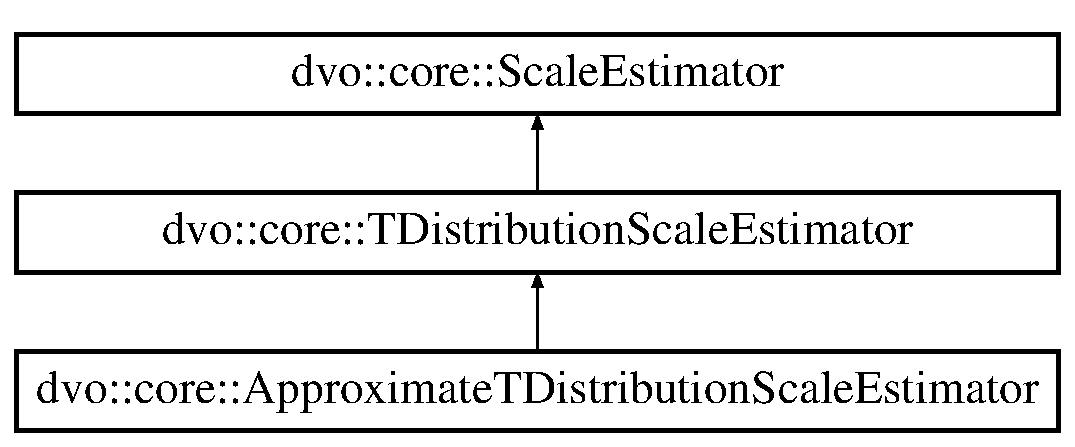
\includegraphics[height=3.000000cm]{classdvo_1_1core_1_1_approximate_t_distribution_scale_estimator}
\end{center}
\end{figure}
\subsection*{Public Member Functions}
\begin{DoxyCompactItemize}
\item 
\mbox{\hyperlink{classdvo_1_1core_1_1_approximate_t_distribution_scale_estimator_aaa8e0b24e62dd26cb712a2253ae47a1c}{Approximate\+T\+Distribution\+Scale\+Estimator}} (const float \mbox{\hyperlink{classdvo_1_1core_1_1_t_distribution_scale_estimator_a4c5ece510a3315bad7ca711a27466eb9}{dof}}=\mbox{\hyperlink{classdvo_1_1core_1_1_t_distribution_scale_estimator_a031ff291023c516c23bce04b34b79957}{D\+E\+F\+A\+U\+L\+T\+\_\+\+D\+OF}})
\item 
virtual \mbox{\hyperlink{classdvo_1_1core_1_1_approximate_t_distribution_scale_estimator_ac87b6733d044e01a947620a79b5368a8}{$\sim$\+Approximate\+T\+Distribution\+Scale\+Estimator}} ()
\item 
virtual float \mbox{\hyperlink{classdvo_1_1core_1_1_approximate_t_distribution_scale_estimator_aee2b37700df1eb0125b8e0d352f7ceab}{compute}} (const cv\+::\+Mat \&errors) const
\end{DoxyCompactItemize}
\subsection*{Additional Inherited Members}


\subsection{Constructor \& Destructor Documentation}
\mbox{\Hypertarget{classdvo_1_1core_1_1_approximate_t_distribution_scale_estimator_aaa8e0b24e62dd26cb712a2253ae47a1c}\label{classdvo_1_1core_1_1_approximate_t_distribution_scale_estimator_aaa8e0b24e62dd26cb712a2253ae47a1c}} 
\index{dvo\+::core\+::\+Approximate\+T\+Distribution\+Scale\+Estimator@{dvo\+::core\+::\+Approximate\+T\+Distribution\+Scale\+Estimator}!Approximate\+T\+Distribution\+Scale\+Estimator@{Approximate\+T\+Distribution\+Scale\+Estimator}}
\index{Approximate\+T\+Distribution\+Scale\+Estimator@{Approximate\+T\+Distribution\+Scale\+Estimator}!dvo\+::core\+::\+Approximate\+T\+Distribution\+Scale\+Estimator@{dvo\+::core\+::\+Approximate\+T\+Distribution\+Scale\+Estimator}}
\subsubsection{\texorpdfstring{Approximate\+T\+Distribution\+Scale\+Estimator()}{ApproximateTDistributionScaleEstimator()}}
{\footnotesize\ttfamily dvo\+::core\+::\+Approximate\+T\+Distribution\+Scale\+Estimator\+::\+Approximate\+T\+Distribution\+Scale\+Estimator (\begin{DoxyParamCaption}\item[{const float}]{dof = {\ttfamily \mbox{\hyperlink{classdvo_1_1core_1_1_t_distribution_scale_estimator_a031ff291023c516c23bce04b34b79957}{D\+E\+F\+A\+U\+L\+T\+\_\+\+D\+OF}}} }\end{DoxyParamCaption})}

\mbox{\Hypertarget{classdvo_1_1core_1_1_approximate_t_distribution_scale_estimator_ac87b6733d044e01a947620a79b5368a8}\label{classdvo_1_1core_1_1_approximate_t_distribution_scale_estimator_ac87b6733d044e01a947620a79b5368a8}} 
\index{dvo\+::core\+::\+Approximate\+T\+Distribution\+Scale\+Estimator@{dvo\+::core\+::\+Approximate\+T\+Distribution\+Scale\+Estimator}!````~Approximate\+T\+Distribution\+Scale\+Estimator@{$\sim$\+Approximate\+T\+Distribution\+Scale\+Estimator}}
\index{````~Approximate\+T\+Distribution\+Scale\+Estimator@{$\sim$\+Approximate\+T\+Distribution\+Scale\+Estimator}!dvo\+::core\+::\+Approximate\+T\+Distribution\+Scale\+Estimator@{dvo\+::core\+::\+Approximate\+T\+Distribution\+Scale\+Estimator}}
\subsubsection{\texorpdfstring{$\sim$\+Approximate\+T\+Distribution\+Scale\+Estimator()}{~ApproximateTDistributionScaleEstimator()}}
{\footnotesize\ttfamily virtual dvo\+::core\+::\+Approximate\+T\+Distribution\+Scale\+Estimator\+::$\sim$\+Approximate\+T\+Distribution\+Scale\+Estimator (\begin{DoxyParamCaption}{ }\end{DoxyParamCaption})\hspace{0.3cm}{\ttfamily [inline]}, {\ttfamily [virtual]}}



\subsection{Member Function Documentation}
\mbox{\Hypertarget{classdvo_1_1core_1_1_approximate_t_distribution_scale_estimator_aee2b37700df1eb0125b8e0d352f7ceab}\label{classdvo_1_1core_1_1_approximate_t_distribution_scale_estimator_aee2b37700df1eb0125b8e0d352f7ceab}} 
\index{dvo\+::core\+::\+Approximate\+T\+Distribution\+Scale\+Estimator@{dvo\+::core\+::\+Approximate\+T\+Distribution\+Scale\+Estimator}!compute@{compute}}
\index{compute@{compute}!dvo\+::core\+::\+Approximate\+T\+Distribution\+Scale\+Estimator@{dvo\+::core\+::\+Approximate\+T\+Distribution\+Scale\+Estimator}}
\subsubsection{\texorpdfstring{compute()}{compute()}}
{\footnotesize\ttfamily float dvo\+::core\+::\+Approximate\+T\+Distribution\+Scale\+Estimator\+::compute (\begin{DoxyParamCaption}\item[{const cv\+::\+Mat \&}]{errors }\end{DoxyParamCaption}) const\hspace{0.3cm}{\ttfamily [virtual]}}



Reimplemented from \mbox{\hyperlink{classdvo_1_1core_1_1_t_distribution_scale_estimator_a0ed88ffeb9b71110e3ae69b681526bc4}{dvo\+::core\+::\+T\+Distribution\+Scale\+Estimator}}.



The documentation for this class was generated from the following files\+:\begin{DoxyCompactItemize}
\item 
dvo\+\_\+core/include/dvo/core/\mbox{\hyperlink{weight__calculation_8h}{weight\+\_\+calculation.\+h}}\item 
dvo\+\_\+core/src/core/\mbox{\hyperlink{weight__calculation_8cpp}{weight\+\_\+calculation.\+cpp}}\end{DoxyCompactItemize}

\hypertarget{classdvo_1_1visualization_1_1_async_point_cloud_builder}{}\section{dvo\+:\+:visualization\+:\+:Async\+Point\+Cloud\+Builder Class Reference}
\label{classdvo_1_1visualization_1_1_async_point_cloud_builder}\index{dvo\+::visualization\+::\+Async\+Point\+Cloud\+Builder@{dvo\+::visualization\+::\+Async\+Point\+Cloud\+Builder}}


{\ttfamily \#include $<$async\+\_\+point\+\_\+cloud\+\_\+builder.\+h$>$}

\subsection*{Classes}
\begin{DoxyCompactItemize}
\item 
struct \mbox{\hyperlink{structdvo_1_1visualization_1_1_async_point_cloud_builder_1_1_build_job}{Build\+Job}}
\end{DoxyCompactItemize}
\subsection*{Public Types}
\begin{DoxyCompactItemize}
\item 
typedef pcl\+::\+Point\+Cloud$<$ pcl\+::\+Point\+X\+Y\+Z\+R\+GB $>$ \mbox{\hyperlink{classdvo_1_1visualization_1_1_async_point_cloud_builder_adbe8a48427924927ac5deaaaf52fe5f3}{Point\+Cloud}}
\item 
typedef boost\+::function$<$ void(const Point\+Cloud\+::\+Ptr \&cloud)$>$ \mbox{\hyperlink{classdvo_1_1visualization_1_1_async_point_cloud_builder_aeea54b24aabbcfe12b2db923c8befc77}{Done\+Callback}}
\end{DoxyCompactItemize}
\subsection*{Public Member Functions}
\begin{DoxyCompactItemize}
\item 
\mbox{\hyperlink{classdvo_1_1visualization_1_1_async_point_cloud_builder_ab070aedbbd9aa5feef1d7808ca40b368}{Async\+Point\+Cloud\+Builder}} ()
\item 
virtual \mbox{\hyperlink{classdvo_1_1visualization_1_1_async_point_cloud_builder_a73217b33adf0d739b98fcec32756a6ed}{$\sim$\+Async\+Point\+Cloud\+Builder}} ()
\item 
void \mbox{\hyperlink{classdvo_1_1visualization_1_1_async_point_cloud_builder_a8347f241fd74e390aedaebfe4ce5c619}{build}} (const \mbox{\hyperlink{structdvo_1_1core_1_1_rgbd_image}{dvo\+::core\+::\+Rgbd\+Image}} \&image, const \mbox{\hyperlink{structdvo_1_1core_1_1_intrinsic_matrix}{dvo\+::core\+::\+Intrinsic\+Matrix}} \&intrinsics, const Eigen\+::\+Affine3d pose=Eigen\+::\+Affine3d\+::\+Identity())
\item 
void \mbox{\hyperlink{classdvo_1_1visualization_1_1_async_point_cloud_builder_a64258774d1203a294842d2a45bccc121}{done}} (\mbox{\hyperlink{classdvo_1_1visualization_1_1_async_point_cloud_builder_aeea54b24aabbcfe12b2db923c8befc77}{Done\+Callback}} \&callback)
\end{DoxyCompactItemize}


\subsection{Member Typedef Documentation}
\mbox{\Hypertarget{classdvo_1_1visualization_1_1_async_point_cloud_builder_aeea54b24aabbcfe12b2db923c8befc77}\label{classdvo_1_1visualization_1_1_async_point_cloud_builder_aeea54b24aabbcfe12b2db923c8befc77}} 
\index{dvo\+::visualization\+::\+Async\+Point\+Cloud\+Builder@{dvo\+::visualization\+::\+Async\+Point\+Cloud\+Builder}!Done\+Callback@{Done\+Callback}}
\index{Done\+Callback@{Done\+Callback}!dvo\+::visualization\+::\+Async\+Point\+Cloud\+Builder@{dvo\+::visualization\+::\+Async\+Point\+Cloud\+Builder}}
\subsubsection{\texorpdfstring{Done\+Callback}{DoneCallback}}
{\footnotesize\ttfamily typedef boost\+::function$<$void (const Point\+Cloud\+::\+Ptr\& cloud)$>$ \mbox{\hyperlink{classdvo_1_1visualization_1_1_async_point_cloud_builder_aeea54b24aabbcfe12b2db923c8befc77}{dvo\+::visualization\+::\+Async\+Point\+Cloud\+Builder\+::\+Done\+Callback}}}

\mbox{\Hypertarget{classdvo_1_1visualization_1_1_async_point_cloud_builder_adbe8a48427924927ac5deaaaf52fe5f3}\label{classdvo_1_1visualization_1_1_async_point_cloud_builder_adbe8a48427924927ac5deaaaf52fe5f3}} 
\index{dvo\+::visualization\+::\+Async\+Point\+Cloud\+Builder@{dvo\+::visualization\+::\+Async\+Point\+Cloud\+Builder}!Point\+Cloud@{Point\+Cloud}}
\index{Point\+Cloud@{Point\+Cloud}!dvo\+::visualization\+::\+Async\+Point\+Cloud\+Builder@{dvo\+::visualization\+::\+Async\+Point\+Cloud\+Builder}}
\subsubsection{\texorpdfstring{Point\+Cloud}{PointCloud}}
{\footnotesize\ttfamily typedef pcl\+::\+Point\+Cloud$<$pcl\+::\+Point\+X\+Y\+Z\+R\+GB$>$ \mbox{\hyperlink{classdvo_1_1visualization_1_1_async_point_cloud_builder_adbe8a48427924927ac5deaaaf52fe5f3}{dvo\+::visualization\+::\+Async\+Point\+Cloud\+Builder\+::\+Point\+Cloud}}}



\subsection{Constructor \& Destructor Documentation}
\mbox{\Hypertarget{classdvo_1_1visualization_1_1_async_point_cloud_builder_ab070aedbbd9aa5feef1d7808ca40b368}\label{classdvo_1_1visualization_1_1_async_point_cloud_builder_ab070aedbbd9aa5feef1d7808ca40b368}} 
\index{dvo\+::visualization\+::\+Async\+Point\+Cloud\+Builder@{dvo\+::visualization\+::\+Async\+Point\+Cloud\+Builder}!Async\+Point\+Cloud\+Builder@{Async\+Point\+Cloud\+Builder}}
\index{Async\+Point\+Cloud\+Builder@{Async\+Point\+Cloud\+Builder}!dvo\+::visualization\+::\+Async\+Point\+Cloud\+Builder@{dvo\+::visualization\+::\+Async\+Point\+Cloud\+Builder}}
\subsubsection{\texorpdfstring{Async\+Point\+Cloud\+Builder()}{AsyncPointCloudBuilder()}}
{\footnotesize\ttfamily dvo\+::visualization\+::\+Async\+Point\+Cloud\+Builder\+::\+Async\+Point\+Cloud\+Builder (\begin{DoxyParamCaption}{ }\end{DoxyParamCaption})}

\mbox{\Hypertarget{classdvo_1_1visualization_1_1_async_point_cloud_builder_a73217b33adf0d739b98fcec32756a6ed}\label{classdvo_1_1visualization_1_1_async_point_cloud_builder_a73217b33adf0d739b98fcec32756a6ed}} 
\index{dvo\+::visualization\+::\+Async\+Point\+Cloud\+Builder@{dvo\+::visualization\+::\+Async\+Point\+Cloud\+Builder}!````~Async\+Point\+Cloud\+Builder@{$\sim$\+Async\+Point\+Cloud\+Builder}}
\index{````~Async\+Point\+Cloud\+Builder@{$\sim$\+Async\+Point\+Cloud\+Builder}!dvo\+::visualization\+::\+Async\+Point\+Cloud\+Builder@{dvo\+::visualization\+::\+Async\+Point\+Cloud\+Builder}}
\subsubsection{\texorpdfstring{$\sim$\+Async\+Point\+Cloud\+Builder()}{~AsyncPointCloudBuilder()}}
{\footnotesize\ttfamily dvo\+::visualization\+::\+Async\+Point\+Cloud\+Builder\+::$\sim$\+Async\+Point\+Cloud\+Builder (\begin{DoxyParamCaption}{ }\end{DoxyParamCaption})\hspace{0.3cm}{\ttfamily [virtual]}}



\subsection{Member Function Documentation}
\mbox{\Hypertarget{classdvo_1_1visualization_1_1_async_point_cloud_builder_a8347f241fd74e390aedaebfe4ce5c619}\label{classdvo_1_1visualization_1_1_async_point_cloud_builder_a8347f241fd74e390aedaebfe4ce5c619}} 
\index{dvo\+::visualization\+::\+Async\+Point\+Cloud\+Builder@{dvo\+::visualization\+::\+Async\+Point\+Cloud\+Builder}!build@{build}}
\index{build@{build}!dvo\+::visualization\+::\+Async\+Point\+Cloud\+Builder@{dvo\+::visualization\+::\+Async\+Point\+Cloud\+Builder}}
\subsubsection{\texorpdfstring{build()}{build()}}
{\footnotesize\ttfamily void dvo\+::visualization\+::\+Async\+Point\+Cloud\+Builder\+::build (\begin{DoxyParamCaption}\item[{const \mbox{\hyperlink{structdvo_1_1core_1_1_rgbd_image}{dvo\+::core\+::\+Rgbd\+Image}} \&}]{image,  }\item[{const \mbox{\hyperlink{structdvo_1_1core_1_1_intrinsic_matrix}{dvo\+::core\+::\+Intrinsic\+Matrix}} \&}]{intrinsics,  }\item[{const Eigen\+::\+Affine3d}]{pose = {\ttfamily Eigen\+:\+:Affine3d\+:\+:Identity()} }\end{DoxyParamCaption})}

\mbox{\Hypertarget{classdvo_1_1visualization_1_1_async_point_cloud_builder_a64258774d1203a294842d2a45bccc121}\label{classdvo_1_1visualization_1_1_async_point_cloud_builder_a64258774d1203a294842d2a45bccc121}} 
\index{dvo\+::visualization\+::\+Async\+Point\+Cloud\+Builder@{dvo\+::visualization\+::\+Async\+Point\+Cloud\+Builder}!done@{done}}
\index{done@{done}!dvo\+::visualization\+::\+Async\+Point\+Cloud\+Builder@{dvo\+::visualization\+::\+Async\+Point\+Cloud\+Builder}}
\subsubsection{\texorpdfstring{done()}{done()}}
{\footnotesize\ttfamily void dvo\+::visualization\+::\+Async\+Point\+Cloud\+Builder\+::done (\begin{DoxyParamCaption}\item[{\mbox{\hyperlink{classdvo_1_1visualization_1_1_async_point_cloud_builder_aeea54b24aabbcfe12b2db923c8befc77}{Done\+Callback}} \&}]{callback }\end{DoxyParamCaption})}



The documentation for this class was generated from the following files\+:\begin{DoxyCompactItemize}
\item 
dvo\+\_\+core/include/dvo/visualization/\mbox{\hyperlink{async__point__cloud__builder_8h}{async\+\_\+point\+\_\+cloud\+\_\+builder.\+h}}\item 
dvo\+\_\+core/src/visualization/\mbox{\hyperlink{async__point__cloud__builder_8cpp}{async\+\_\+point\+\_\+cloud\+\_\+builder.\+cpp}}\end{DoxyCompactItemize}

\hypertarget{class_benchmark_node}{}\section{Benchmark\+Node Class Reference}
\label{class_benchmark_node}\index{Benchmark\+Node@{Benchmark\+Node}}
\subsection*{Classes}
\begin{DoxyCompactItemize}
\item 
struct \mbox{\hyperlink{struct_benchmark_node_1_1_config}{Config}}
\end{DoxyCompactItemize}
\subsection*{Public Member Functions}
\begin{DoxyCompactItemize}
\item 
\mbox{\hyperlink{class_benchmark_node_ad4ee7b497428bce6426add3c4010200e}{Benchmark\+Node}} (ros\+::\+Node\+Handle \&nh, ros\+::\+Node\+Handle \&nh\+\_\+private)
\item 
bool \mbox{\hyperlink{class_benchmark_node_a6fb208304f873fb46988f6ca4ed0b9d8}{configure}} ()
\item 
void \mbox{\hyperlink{class_benchmark_node_a4f509351e1c61f174f64146fe3abb463}{run}} ()
\item 
void \mbox{\hyperlink{class_benchmark_node_ac906f068111a96dc95b289d3728df574}{create\+Reference\+Camera}} (\mbox{\hyperlink{classdvo_1_1visualization_1_1_camera_trajectory_visualizer_interface}{dvo\+::visualization\+::\+Camera\+Trajectory\+Visualizer\+Interface}} $\ast$visualizer, const \mbox{\hyperlink{structdvo_1_1core_1_1_rgbd_image}{dvo\+::core\+::\+Rgbd\+Image}} \&img, const \mbox{\hyperlink{structdvo_1_1core_1_1_intrinsic_matrix}{dvo\+::core\+::\+Intrinsic\+Matrix}} \&intrinsics, const Eigen\+::\+Affine3d \&pose)
\item 
void \mbox{\hyperlink{class_benchmark_node_aa8ac48849e2165f15af69e561ecb97e6}{render\+While\+Switch\+And\+Not\+Terminated}} (\mbox{\hyperlink{classdvo_1_1visualization_1_1_camera_trajectory_visualizer_interface}{dvo\+::visualization\+::\+Camera\+Trajectory\+Visualizer\+Interface}} $\ast$visualizer, const \mbox{\hyperlink{structdvo_1_1visualization_1_1_switch}{dvo\+::visualization\+::\+Switch}} \&s)
\item 
void \mbox{\hyperlink{class_benchmark_node_a81ccf22ce05702c97803a502092090f7}{process\+Input}} (\mbox{\hyperlink{classdvo_1_1visualization_1_1_camera_trajectory_visualizer_interface}{dvo\+::visualization\+::\+Camera\+Trajectory\+Visualizer\+Interface}} $\ast$visualizer)
\end{DoxyCompactItemize}


\subsection{Constructor \& Destructor Documentation}
\mbox{\Hypertarget{class_benchmark_node_ad4ee7b497428bce6426add3c4010200e}\label{class_benchmark_node_ad4ee7b497428bce6426add3c4010200e}} 
\index{Benchmark\+Node@{Benchmark\+Node}!Benchmark\+Node@{Benchmark\+Node}}
\index{Benchmark\+Node@{Benchmark\+Node}!Benchmark\+Node@{Benchmark\+Node}}
\subsubsection{\texorpdfstring{Benchmark\+Node()}{BenchmarkNode()}}
{\footnotesize\ttfamily Benchmark\+Node\+::\+Benchmark\+Node (\begin{DoxyParamCaption}\item[{ros\+::\+Node\+Handle \&}]{nh,  }\item[{ros\+::\+Node\+Handle \&}]{nh\+\_\+private }\end{DoxyParamCaption})}



\subsection{Member Function Documentation}
\mbox{\Hypertarget{class_benchmark_node_a6fb208304f873fb46988f6ca4ed0b9d8}\label{class_benchmark_node_a6fb208304f873fb46988f6ca4ed0b9d8}} 
\index{Benchmark\+Node@{Benchmark\+Node}!configure@{configure}}
\index{configure@{configure}!Benchmark\+Node@{Benchmark\+Node}}
\subsubsection{\texorpdfstring{configure()}{configure()}}
{\footnotesize\ttfamily bool Benchmark\+Node\+::configure (\begin{DoxyParamCaption}{ }\end{DoxyParamCaption})}

configure stuff like\+:
\begin{DoxyEnumerate}
\item rgbdpair files,
\item trajectory estimation (if you want to use tum tools to estimate the trajectory)
\item video rendering stuff.
\item show ground truth. 
\end{DoxyEnumerate}\mbox{\Hypertarget{class_benchmark_node_ac906f068111a96dc95b289d3728df574}\label{class_benchmark_node_ac906f068111a96dc95b289d3728df574}} 
\index{Benchmark\+Node@{Benchmark\+Node}!create\+Reference\+Camera@{create\+Reference\+Camera}}
\index{create\+Reference\+Camera@{create\+Reference\+Camera}!Benchmark\+Node@{Benchmark\+Node}}
\subsubsection{\texorpdfstring{create\+Reference\+Camera()}{createReferenceCamera()}}
{\footnotesize\ttfamily void Benchmark\+Node\+::create\+Reference\+Camera (\begin{DoxyParamCaption}\item[{\mbox{\hyperlink{classdvo_1_1visualization_1_1_camera_trajectory_visualizer_interface}{dvo\+::visualization\+::\+Camera\+Trajectory\+Visualizer\+Interface}} $\ast$}]{visualizer,  }\item[{const \mbox{\hyperlink{structdvo_1_1core_1_1_rgbd_image}{dvo\+::core\+::\+Rgbd\+Image}} \&}]{img,  }\item[{const \mbox{\hyperlink{structdvo_1_1core_1_1_intrinsic_matrix}{dvo\+::core\+::\+Intrinsic\+Matrix}} \&}]{intrinsics,  }\item[{const Eigen\+::\+Affine3d \&}]{pose }\end{DoxyParamCaption})}

\mbox{\Hypertarget{class_benchmark_node_a81ccf22ce05702c97803a502092090f7}\label{class_benchmark_node_a81ccf22ce05702c97803a502092090f7}} 
\index{Benchmark\+Node@{Benchmark\+Node}!process\+Input@{process\+Input}}
\index{process\+Input@{process\+Input}!Benchmark\+Node@{Benchmark\+Node}}
\subsubsection{\texorpdfstring{process\+Input()}{processInput()}}
{\footnotesize\ttfamily void Benchmark\+Node\+::process\+Input (\begin{DoxyParamCaption}\item[{\mbox{\hyperlink{classdvo_1_1visualization_1_1_camera_trajectory_visualizer_interface}{dvo\+::visualization\+::\+Camera\+Trajectory\+Visualizer\+Interface}} $\ast$}]{visualizer }\end{DoxyParamCaption})}


\begin{DoxyEnumerate}
\item saving the camera pose file to disk
\item or load cmera pose from file 
\end{DoxyEnumerate}\mbox{\Hypertarget{class_benchmark_node_aa8ac48849e2165f15af69e561ecb97e6}\label{class_benchmark_node_aa8ac48849e2165f15af69e561ecb97e6}} 
\index{Benchmark\+Node@{Benchmark\+Node}!render\+While\+Switch\+And\+Not\+Terminated@{render\+While\+Switch\+And\+Not\+Terminated}}
\index{render\+While\+Switch\+And\+Not\+Terminated@{render\+While\+Switch\+And\+Not\+Terminated}!Benchmark\+Node@{Benchmark\+Node}}
\subsubsection{\texorpdfstring{render\+While\+Switch\+And\+Not\+Terminated()}{renderWhileSwitchAndNotTerminated()}}
{\footnotesize\ttfamily void Benchmark\+Node\+::render\+While\+Switch\+And\+Not\+Terminated (\begin{DoxyParamCaption}\item[{\mbox{\hyperlink{classdvo_1_1visualization_1_1_camera_trajectory_visualizer_interface}{dvo\+::visualization\+::\+Camera\+Trajectory\+Visualizer\+Interface}} $\ast$}]{visualizer,  }\item[{const \mbox{\hyperlink{structdvo_1_1visualization_1_1_switch}{dvo\+::visualization\+::\+Switch}} \&}]{s }\end{DoxyParamCaption})}

continuously calling the visualizer to render, on and on... (5\+Hz) Please refer to the \mbox{\hyperlink{classdvo_1_1visualization_1_1_pcl_camera_trajectory_visualizer}{dvo\+::visualization\+::\+Pcl\+Camera\+Trajectory\+Visualizer}} to see what this function is actually doing. \mbox{\Hypertarget{class_benchmark_node_a4f509351e1c61f174f64146fe3abb463}\label{class_benchmark_node_a4f509351e1c61f174f64146fe3abb463}} 
\index{Benchmark\+Node@{Benchmark\+Node}!run@{run}}
\index{run@{run}!Benchmark\+Node@{Benchmark\+Node}}
\subsubsection{\texorpdfstring{run()}{run()}}
{\footnotesize\ttfamily void Benchmark\+Node\+::run (\begin{DoxyParamCaption}{ }\end{DoxyParamCaption})}

The most important funciton in \mbox{\hyperlink{class_benchmark_node}{Benchmark\+Node}}.
\begin{DoxyEnumerate}
\item setup the visualizer
\item generate id for each frame in the Video\+Folder.
\item (configure debugging visualizer)
\item setup camera parameters (create intrinsic\+Matrix)
\item setup configuration for tracker node (class Camera\+Dense\+Tracker\+Config) from server, and output in R\+OS warning.
\item initialize first pose
\item read all rgb-\/d pair entries
\item start iteration\+: 8.\+1 create Reference Camera and do something about visualization 8.\+2 if Estimate is Required, then call dense\+\_\+tracker.\+match($\ast$reference, $\ast$current, relative)
\item if Show\+Estimate or Render\+Video is set in cfg\+\_\+, then do it. 
\end{DoxyEnumerate}

The documentation for this class was generated from the following file\+:\begin{DoxyCompactItemize}
\item 
dvo\+\_\+benchmark/src/\mbox{\hyperlink{benchmark_8cpp}{benchmark.\+cpp}}\end{DoxyCompactItemize}

\hypertarget{classdvo_1_1visualization_1_1bounded__buffer}{}\section{dvo\+:\+:visualization\+:\+:bounded\+\_\+buffer$<$ T $>$ Class Template Reference}
\label{classdvo_1_1visualization_1_1bounded__buffer}\index{dvo\+::visualization\+::bounded\+\_\+buffer$<$ T $>$@{dvo\+::visualization\+::bounded\+\_\+buffer$<$ T $>$}}


{\ttfamily \#include $<$bounded\+\_\+buffer.\+h$>$}

\subsection*{Public Types}
\begin{DoxyCompactItemize}
\item 
typedef boost\+::circular\+\_\+buffer$<$ T $>$ \mbox{\hyperlink{classdvo_1_1visualization_1_1bounded__buffer_aaeb9b2a645cb183a85167be95f09745b}{container\+\_\+type}}
\item 
typedef container\+\_\+type\+::size\+\_\+type \mbox{\hyperlink{classdvo_1_1visualization_1_1bounded__buffer_a0b8808bbfd4de59ebf33d5241083179c}{size\+\_\+type}}
\item 
typedef container\+\_\+type\+::value\+\_\+type \mbox{\hyperlink{classdvo_1_1visualization_1_1bounded__buffer_a69f22957276557660f1bf8b654e3a667}{value\+\_\+type}}
\end{DoxyCompactItemize}
\subsection*{Public Member Functions}
\begin{DoxyCompactItemize}
\item 
\mbox{\hyperlink{classdvo_1_1visualization_1_1bounded__buffer_a392dce467c80a3b980be50ed2f538181}{bounded\+\_\+buffer}} (\mbox{\hyperlink{classdvo_1_1visualization_1_1bounded__buffer_a0b8808bbfd4de59ebf33d5241083179c}{size\+\_\+type}} capacity)
\item 
void \mbox{\hyperlink{classdvo_1_1visualization_1_1bounded__buffer_a2b72854b9be8a3c4831f9f46d2c4a549}{push\+\_\+front}} (typename container\+\_\+type\+::param\+\_\+value\+\_\+type item)
\item 
bool \mbox{\hyperlink{classdvo_1_1visualization_1_1bounded__buffer_a86bb8a4d2211061d0dda2cbf9a9a82e7}{pop\+\_\+back}} (\mbox{\hyperlink{classdvo_1_1visualization_1_1bounded__buffer_a69f22957276557660f1bf8b654e3a667}{value\+\_\+type}} $\ast$p\+Item)
\item 
void \mbox{\hyperlink{classdvo_1_1visualization_1_1bounded__buffer_ae4afdb9c626f4f38cbc34b81fdfa8bf7}{shutdown}} ()
\end{DoxyCompactItemize}


\subsection{Member Typedef Documentation}
\mbox{\Hypertarget{classdvo_1_1visualization_1_1bounded__buffer_aaeb9b2a645cb183a85167be95f09745b}\label{classdvo_1_1visualization_1_1bounded__buffer_aaeb9b2a645cb183a85167be95f09745b}} 
\index{dvo\+::visualization\+::bounded\+\_\+buffer@{dvo\+::visualization\+::bounded\+\_\+buffer}!container\+\_\+type@{container\+\_\+type}}
\index{container\+\_\+type@{container\+\_\+type}!dvo\+::visualization\+::bounded\+\_\+buffer@{dvo\+::visualization\+::bounded\+\_\+buffer}}
\subsubsection{\texorpdfstring{container\+\_\+type}{container\_type}}
{\footnotesize\ttfamily template$<$class T$>$ \\
typedef boost\+::circular\+\_\+buffer$<$T$>$ \mbox{\hyperlink{classdvo_1_1visualization_1_1bounded__buffer}{dvo\+::visualization\+::bounded\+\_\+buffer}}$<$ T $>$\+::\mbox{\hyperlink{classdvo_1_1visualization_1_1bounded__buffer_aaeb9b2a645cb183a85167be95f09745b}{container\+\_\+type}}}

\mbox{\Hypertarget{classdvo_1_1visualization_1_1bounded__buffer_a0b8808bbfd4de59ebf33d5241083179c}\label{classdvo_1_1visualization_1_1bounded__buffer_a0b8808bbfd4de59ebf33d5241083179c}} 
\index{dvo\+::visualization\+::bounded\+\_\+buffer@{dvo\+::visualization\+::bounded\+\_\+buffer}!size\+\_\+type@{size\+\_\+type}}
\index{size\+\_\+type@{size\+\_\+type}!dvo\+::visualization\+::bounded\+\_\+buffer@{dvo\+::visualization\+::bounded\+\_\+buffer}}
\subsubsection{\texorpdfstring{size\+\_\+type}{size\_type}}
{\footnotesize\ttfamily template$<$class T$>$ \\
typedef container\+\_\+type\+::size\+\_\+type \mbox{\hyperlink{classdvo_1_1visualization_1_1bounded__buffer}{dvo\+::visualization\+::bounded\+\_\+buffer}}$<$ T $>$\+::\mbox{\hyperlink{classdvo_1_1visualization_1_1bounded__buffer_a0b8808bbfd4de59ebf33d5241083179c}{size\+\_\+type}}}

\mbox{\Hypertarget{classdvo_1_1visualization_1_1bounded__buffer_a69f22957276557660f1bf8b654e3a667}\label{classdvo_1_1visualization_1_1bounded__buffer_a69f22957276557660f1bf8b654e3a667}} 
\index{dvo\+::visualization\+::bounded\+\_\+buffer@{dvo\+::visualization\+::bounded\+\_\+buffer}!value\+\_\+type@{value\+\_\+type}}
\index{value\+\_\+type@{value\+\_\+type}!dvo\+::visualization\+::bounded\+\_\+buffer@{dvo\+::visualization\+::bounded\+\_\+buffer}}
\subsubsection{\texorpdfstring{value\+\_\+type}{value\_type}}
{\footnotesize\ttfamily template$<$class T$>$ \\
typedef container\+\_\+type\+::value\+\_\+type \mbox{\hyperlink{classdvo_1_1visualization_1_1bounded__buffer}{dvo\+::visualization\+::bounded\+\_\+buffer}}$<$ T $>$\+::\mbox{\hyperlink{classdvo_1_1visualization_1_1bounded__buffer_a69f22957276557660f1bf8b654e3a667}{value\+\_\+type}}}



\subsection{Constructor \& Destructor Documentation}
\mbox{\Hypertarget{classdvo_1_1visualization_1_1bounded__buffer_a392dce467c80a3b980be50ed2f538181}\label{classdvo_1_1visualization_1_1bounded__buffer_a392dce467c80a3b980be50ed2f538181}} 
\index{dvo\+::visualization\+::bounded\+\_\+buffer@{dvo\+::visualization\+::bounded\+\_\+buffer}!bounded\+\_\+buffer@{bounded\+\_\+buffer}}
\index{bounded\+\_\+buffer@{bounded\+\_\+buffer}!dvo\+::visualization\+::bounded\+\_\+buffer@{dvo\+::visualization\+::bounded\+\_\+buffer}}
\subsubsection{\texorpdfstring{bounded\+\_\+buffer()}{bounded\_buffer()}}
{\footnotesize\ttfamily template$<$class T$>$ \\
\mbox{\hyperlink{classdvo_1_1visualization_1_1bounded__buffer}{dvo\+::visualization\+::bounded\+\_\+buffer}}$<$ T $>$\+::\mbox{\hyperlink{classdvo_1_1visualization_1_1bounded__buffer}{bounded\+\_\+buffer}} (\begin{DoxyParamCaption}\item[{\mbox{\hyperlink{classdvo_1_1visualization_1_1bounded__buffer_a0b8808bbfd4de59ebf33d5241083179c}{size\+\_\+type}}}]{capacity }\end{DoxyParamCaption})\hspace{0.3cm}{\ttfamily [inline]}, {\ttfamily [explicit]}}



\subsection{Member Function Documentation}
\mbox{\Hypertarget{classdvo_1_1visualization_1_1bounded__buffer_a86bb8a4d2211061d0dda2cbf9a9a82e7}\label{classdvo_1_1visualization_1_1bounded__buffer_a86bb8a4d2211061d0dda2cbf9a9a82e7}} 
\index{dvo\+::visualization\+::bounded\+\_\+buffer@{dvo\+::visualization\+::bounded\+\_\+buffer}!pop\+\_\+back@{pop\+\_\+back}}
\index{pop\+\_\+back@{pop\+\_\+back}!dvo\+::visualization\+::bounded\+\_\+buffer@{dvo\+::visualization\+::bounded\+\_\+buffer}}
\subsubsection{\texorpdfstring{pop\+\_\+back()}{pop\_back()}}
{\footnotesize\ttfamily template$<$class T$>$ \\
bool \mbox{\hyperlink{classdvo_1_1visualization_1_1bounded__buffer}{dvo\+::visualization\+::bounded\+\_\+buffer}}$<$ T $>$\+::pop\+\_\+back (\begin{DoxyParamCaption}\item[{\mbox{\hyperlink{classdvo_1_1visualization_1_1bounded__buffer_a69f22957276557660f1bf8b654e3a667}{value\+\_\+type}} $\ast$}]{p\+Item }\end{DoxyParamCaption})\hspace{0.3cm}{\ttfamily [inline]}}

\mbox{\Hypertarget{classdvo_1_1visualization_1_1bounded__buffer_a2b72854b9be8a3c4831f9f46d2c4a549}\label{classdvo_1_1visualization_1_1bounded__buffer_a2b72854b9be8a3c4831f9f46d2c4a549}} 
\index{dvo\+::visualization\+::bounded\+\_\+buffer@{dvo\+::visualization\+::bounded\+\_\+buffer}!push\+\_\+front@{push\+\_\+front}}
\index{push\+\_\+front@{push\+\_\+front}!dvo\+::visualization\+::bounded\+\_\+buffer@{dvo\+::visualization\+::bounded\+\_\+buffer}}
\subsubsection{\texorpdfstring{push\+\_\+front()}{push\_front()}}
{\footnotesize\ttfamily template$<$class T$>$ \\
void \mbox{\hyperlink{classdvo_1_1visualization_1_1bounded__buffer}{dvo\+::visualization\+::bounded\+\_\+buffer}}$<$ T $>$\+::push\+\_\+front (\begin{DoxyParamCaption}\item[{typename container\+\_\+type\+::param\+\_\+value\+\_\+type}]{item }\end{DoxyParamCaption})\hspace{0.3cm}{\ttfamily [inline]}}

\mbox{\Hypertarget{classdvo_1_1visualization_1_1bounded__buffer_ae4afdb9c626f4f38cbc34b81fdfa8bf7}\label{classdvo_1_1visualization_1_1bounded__buffer_ae4afdb9c626f4f38cbc34b81fdfa8bf7}} 
\index{dvo\+::visualization\+::bounded\+\_\+buffer@{dvo\+::visualization\+::bounded\+\_\+buffer}!shutdown@{shutdown}}
\index{shutdown@{shutdown}!dvo\+::visualization\+::bounded\+\_\+buffer@{dvo\+::visualization\+::bounded\+\_\+buffer}}
\subsubsection{\texorpdfstring{shutdown()}{shutdown()}}
{\footnotesize\ttfamily template$<$class T$>$ \\
void \mbox{\hyperlink{classdvo_1_1visualization_1_1bounded__buffer}{dvo\+::visualization\+::bounded\+\_\+buffer}}$<$ T $>$\+::shutdown (\begin{DoxyParamCaption}{ }\end{DoxyParamCaption})\hspace{0.3cm}{\ttfamily [inline]}}



The documentation for this class was generated from the following file\+:\begin{DoxyCompactItemize}
\item 
dvo\+\_\+core/src/visualization/\mbox{\hyperlink{bounded__buffer_8h}{bounded\+\_\+buffer.\+h}}\end{DoxyCompactItemize}

\hypertarget{structdvo_1_1visualization_1_1_async_point_cloud_builder_1_1_build_job}{}\section{dvo\+:\+:visualization\+:\+:Async\+Point\+Cloud\+Builder\+:\+:Build\+Job Struct Reference}
\label{structdvo_1_1visualization_1_1_async_point_cloud_builder_1_1_build_job}\index{dvo\+::visualization\+::\+Async\+Point\+Cloud\+Builder\+::\+Build\+Job@{dvo\+::visualization\+::\+Async\+Point\+Cloud\+Builder\+::\+Build\+Job}}


{\ttfamily \#include $<$async\+\_\+point\+\_\+cloud\+\_\+builder.\+h$>$}

\subsection*{Public Member Functions}
\begin{DoxyCompactItemize}
\item 
\mbox{\hyperlink{structdvo_1_1visualization_1_1_async_point_cloud_builder_1_1_build_job_aec73b6b369dcca8f963192af75c3a47e}{Build\+Job}} (const \mbox{\hyperlink{structdvo_1_1core_1_1_rgbd_image}{dvo\+::core\+::\+Rgbd\+Image}} \&\mbox{\hyperlink{structdvo_1_1visualization_1_1_async_point_cloud_builder_1_1_build_job_a72ca6499e953f81647aa4f3bf784f3be}{image}}, const \mbox{\hyperlink{structdvo_1_1core_1_1_intrinsic_matrix}{dvo\+::core\+::\+Intrinsic\+Matrix}} \&\mbox{\hyperlink{structdvo_1_1visualization_1_1_async_point_cloud_builder_1_1_build_job_a49c37651ffed4860b90907836cc0e362}{intrinsics}}, const Eigen\+::\+Affine3d \mbox{\hyperlink{structdvo_1_1visualization_1_1_async_point_cloud_builder_1_1_build_job_a8a72a1adf7299f22ee95e14e608ad332}{pose}}=Eigen\+::\+Affine3d\+::\+Identity())
\item 
Async\+Point\+Cloud\+Builder\+::\+Point\+Cloud\+::\+Ptr \mbox{\hyperlink{structdvo_1_1visualization_1_1_async_point_cloud_builder_1_1_build_job_a0bd1cdd7ef431814573eac7d0af60f93}{build}} ()
\end{DoxyCompactItemize}
\subsection*{Public Attributes}
\begin{DoxyCompactItemize}
\item 
\mbox{\hyperlink{structdvo_1_1core_1_1_rgbd_image}{dvo\+::core\+::\+Rgbd\+Image}} \mbox{\hyperlink{structdvo_1_1visualization_1_1_async_point_cloud_builder_1_1_build_job_a72ca6499e953f81647aa4f3bf784f3be}{image}}
\item 
const \mbox{\hyperlink{structdvo_1_1core_1_1_intrinsic_matrix}{dvo\+::core\+::\+Intrinsic\+Matrix}} \mbox{\hyperlink{structdvo_1_1visualization_1_1_async_point_cloud_builder_1_1_build_job_a49c37651ffed4860b90907836cc0e362}{intrinsics}}
\item 
const Eigen\+::\+Affine3d \mbox{\hyperlink{structdvo_1_1visualization_1_1_async_point_cloud_builder_1_1_build_job_a8a72a1adf7299f22ee95e14e608ad332}{pose}}
\end{DoxyCompactItemize}


\subsection{Constructor \& Destructor Documentation}
\mbox{\Hypertarget{structdvo_1_1visualization_1_1_async_point_cloud_builder_1_1_build_job_aec73b6b369dcca8f963192af75c3a47e}\label{structdvo_1_1visualization_1_1_async_point_cloud_builder_1_1_build_job_aec73b6b369dcca8f963192af75c3a47e}} 
\index{dvo\+::visualization\+::\+Async\+Point\+Cloud\+Builder\+::\+Build\+Job@{dvo\+::visualization\+::\+Async\+Point\+Cloud\+Builder\+::\+Build\+Job}!Build\+Job@{Build\+Job}}
\index{Build\+Job@{Build\+Job}!dvo\+::visualization\+::\+Async\+Point\+Cloud\+Builder\+::\+Build\+Job@{dvo\+::visualization\+::\+Async\+Point\+Cloud\+Builder\+::\+Build\+Job}}
\subsubsection{\texorpdfstring{Build\+Job()}{BuildJob()}}
{\footnotesize\ttfamily dvo\+::visualization\+::\+Async\+Point\+Cloud\+Builder\+::\+Build\+Job\+::\+Build\+Job (\begin{DoxyParamCaption}\item[{const \mbox{\hyperlink{structdvo_1_1core_1_1_rgbd_image}{dvo\+::core\+::\+Rgbd\+Image}} \&}]{image,  }\item[{const \mbox{\hyperlink{structdvo_1_1core_1_1_intrinsic_matrix}{dvo\+::core\+::\+Intrinsic\+Matrix}} \&}]{intrinsics,  }\item[{const Eigen\+::\+Affine3d}]{pose = {\ttfamily Eigen\+:\+:Affine3d\+:\+:Identity()} }\end{DoxyParamCaption})}



\subsection{Member Function Documentation}
\mbox{\Hypertarget{structdvo_1_1visualization_1_1_async_point_cloud_builder_1_1_build_job_a0bd1cdd7ef431814573eac7d0af60f93}\label{structdvo_1_1visualization_1_1_async_point_cloud_builder_1_1_build_job_a0bd1cdd7ef431814573eac7d0af60f93}} 
\index{dvo\+::visualization\+::\+Async\+Point\+Cloud\+Builder\+::\+Build\+Job@{dvo\+::visualization\+::\+Async\+Point\+Cloud\+Builder\+::\+Build\+Job}!build@{build}}
\index{build@{build}!dvo\+::visualization\+::\+Async\+Point\+Cloud\+Builder\+::\+Build\+Job@{dvo\+::visualization\+::\+Async\+Point\+Cloud\+Builder\+::\+Build\+Job}}
\subsubsection{\texorpdfstring{build()}{build()}}
{\footnotesize\ttfamily Async\+Point\+Cloud\+Builder\+::\+Point\+Cloud\+::\+Ptr dvo\+::visualization\+::\+Async\+Point\+Cloud\+Builder\+::\+Build\+Job\+::build (\begin{DoxyParamCaption}{ }\end{DoxyParamCaption})}



\subsection{Member Data Documentation}
\mbox{\Hypertarget{structdvo_1_1visualization_1_1_async_point_cloud_builder_1_1_build_job_a72ca6499e953f81647aa4f3bf784f3be}\label{structdvo_1_1visualization_1_1_async_point_cloud_builder_1_1_build_job_a72ca6499e953f81647aa4f3bf784f3be}} 
\index{dvo\+::visualization\+::\+Async\+Point\+Cloud\+Builder\+::\+Build\+Job@{dvo\+::visualization\+::\+Async\+Point\+Cloud\+Builder\+::\+Build\+Job}!image@{image}}
\index{image@{image}!dvo\+::visualization\+::\+Async\+Point\+Cloud\+Builder\+::\+Build\+Job@{dvo\+::visualization\+::\+Async\+Point\+Cloud\+Builder\+::\+Build\+Job}}
\subsubsection{\texorpdfstring{image}{image}}
{\footnotesize\ttfamily \mbox{\hyperlink{structdvo_1_1core_1_1_rgbd_image}{dvo\+::core\+::\+Rgbd\+Image}} dvo\+::visualization\+::\+Async\+Point\+Cloud\+Builder\+::\+Build\+Job\+::image}

\mbox{\Hypertarget{structdvo_1_1visualization_1_1_async_point_cloud_builder_1_1_build_job_a49c37651ffed4860b90907836cc0e362}\label{structdvo_1_1visualization_1_1_async_point_cloud_builder_1_1_build_job_a49c37651ffed4860b90907836cc0e362}} 
\index{dvo\+::visualization\+::\+Async\+Point\+Cloud\+Builder\+::\+Build\+Job@{dvo\+::visualization\+::\+Async\+Point\+Cloud\+Builder\+::\+Build\+Job}!intrinsics@{intrinsics}}
\index{intrinsics@{intrinsics}!dvo\+::visualization\+::\+Async\+Point\+Cloud\+Builder\+::\+Build\+Job@{dvo\+::visualization\+::\+Async\+Point\+Cloud\+Builder\+::\+Build\+Job}}
\subsubsection{\texorpdfstring{intrinsics}{intrinsics}}
{\footnotesize\ttfamily const \mbox{\hyperlink{structdvo_1_1core_1_1_intrinsic_matrix}{dvo\+::core\+::\+Intrinsic\+Matrix}} dvo\+::visualization\+::\+Async\+Point\+Cloud\+Builder\+::\+Build\+Job\+::intrinsics}

\mbox{\Hypertarget{structdvo_1_1visualization_1_1_async_point_cloud_builder_1_1_build_job_a8a72a1adf7299f22ee95e14e608ad332}\label{structdvo_1_1visualization_1_1_async_point_cloud_builder_1_1_build_job_a8a72a1adf7299f22ee95e14e608ad332}} 
\index{dvo\+::visualization\+::\+Async\+Point\+Cloud\+Builder\+::\+Build\+Job@{dvo\+::visualization\+::\+Async\+Point\+Cloud\+Builder\+::\+Build\+Job}!pose@{pose}}
\index{pose@{pose}!dvo\+::visualization\+::\+Async\+Point\+Cloud\+Builder\+::\+Build\+Job@{dvo\+::visualization\+::\+Async\+Point\+Cloud\+Builder\+::\+Build\+Job}}
\subsubsection{\texorpdfstring{pose}{pose}}
{\footnotesize\ttfamily const Eigen\+::\+Affine3d dvo\+::visualization\+::\+Async\+Point\+Cloud\+Builder\+::\+Build\+Job\+::pose}



The documentation for this struct was generated from the following files\+:\begin{DoxyCompactItemize}
\item 
dvo\+\_\+core/include/dvo/visualization/\mbox{\hyperlink{async__point__cloud__builder_8h}{async\+\_\+point\+\_\+cloud\+\_\+builder.\+h}}\item 
dvo\+\_\+core/src/visualization/\mbox{\hyperlink{async__point__cloud__builder_8cpp}{async\+\_\+point\+\_\+cloud\+\_\+builder.\+cpp}}\end{DoxyCompactItemize}

\hypertarget{classdvo_1_1visualization_1_1_build_point_cloud_task}{}\section{dvo\+:\+:visualization\+:\+:Build\+Point\+Cloud\+Task Class Reference}
\label{classdvo_1_1visualization_1_1_build_point_cloud_task}\index{dvo\+::visualization\+::\+Build\+Point\+Cloud\+Task@{dvo\+::visualization\+::\+Build\+Point\+Cloud\+Task}}
Inheritance diagram for dvo\+:\+:visualization\+:\+:Build\+Point\+Cloud\+Task\+:\begin{figure}[H]
\begin{center}
\leavevmode
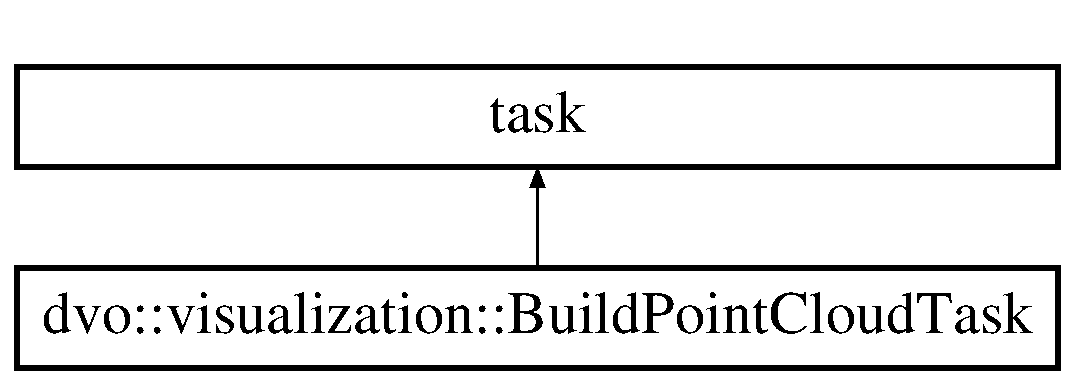
\includegraphics[height=2.000000cm]{classdvo_1_1visualization_1_1_build_point_cloud_task}
\end{center}
\end{figure}
\subsection*{Public Member Functions}
\begin{DoxyCompactItemize}
\item 
\mbox{\hyperlink{classdvo_1_1visualization_1_1_build_point_cloud_task_a86d5efbdab6f61d69949d86291a568ee}{Build\+Point\+Cloud\+Task}} (const \mbox{\hyperlink{structdvo_1_1core_1_1_rgbd_image}{dvo\+::core\+::\+Rgbd\+Image}} \&image, const \mbox{\hyperlink{structdvo_1_1core_1_1_intrinsic_matrix}{dvo\+::core\+::\+Intrinsic\+Matrix}} \&intrinsics, const Eigen\+::\+Affine3d \&pose, \mbox{\hyperlink{classdvo_1_1visualization_1_1_async_point_cloud_builder_aeea54b24aabbcfe12b2db923c8befc77}{Async\+Point\+Cloud\+Builder\+::\+Done\+Callback}} \&callback)
\item 
virtual \mbox{\hyperlink{classdvo_1_1visualization_1_1_build_point_cloud_task_a36ec8829378677b87aca9dd3ef9c5a68}{$\sim$\+Build\+Point\+Cloud\+Task}} ()
\item 
virtual tbb\+::task $\ast$ \mbox{\hyperlink{classdvo_1_1visualization_1_1_build_point_cloud_task_aa9ee4ddd7a6ed4fda80328ed542b7f03}{execute}} ()
\end{DoxyCompactItemize}


\subsection{Constructor \& Destructor Documentation}
\mbox{\Hypertarget{classdvo_1_1visualization_1_1_build_point_cloud_task_a86d5efbdab6f61d69949d86291a568ee}\label{classdvo_1_1visualization_1_1_build_point_cloud_task_a86d5efbdab6f61d69949d86291a568ee}} 
\index{dvo\+::visualization\+::\+Build\+Point\+Cloud\+Task@{dvo\+::visualization\+::\+Build\+Point\+Cloud\+Task}!Build\+Point\+Cloud\+Task@{Build\+Point\+Cloud\+Task}}
\index{Build\+Point\+Cloud\+Task@{Build\+Point\+Cloud\+Task}!dvo\+::visualization\+::\+Build\+Point\+Cloud\+Task@{dvo\+::visualization\+::\+Build\+Point\+Cloud\+Task}}
\subsubsection{\texorpdfstring{Build\+Point\+Cloud\+Task()}{BuildPointCloudTask()}}
{\footnotesize\ttfamily dvo\+::visualization\+::\+Build\+Point\+Cloud\+Task\+::\+Build\+Point\+Cloud\+Task (\begin{DoxyParamCaption}\item[{const \mbox{\hyperlink{structdvo_1_1core_1_1_rgbd_image}{dvo\+::core\+::\+Rgbd\+Image}} \&}]{image,  }\item[{const \mbox{\hyperlink{structdvo_1_1core_1_1_intrinsic_matrix}{dvo\+::core\+::\+Intrinsic\+Matrix}} \&}]{intrinsics,  }\item[{const Eigen\+::\+Affine3d \&}]{pose,  }\item[{\mbox{\hyperlink{classdvo_1_1visualization_1_1_async_point_cloud_builder_aeea54b24aabbcfe12b2db923c8befc77}{Async\+Point\+Cloud\+Builder\+::\+Done\+Callback}} \&}]{callback }\end{DoxyParamCaption})\hspace{0.3cm}{\ttfamily [inline]}}

\mbox{\Hypertarget{classdvo_1_1visualization_1_1_build_point_cloud_task_a36ec8829378677b87aca9dd3ef9c5a68}\label{classdvo_1_1visualization_1_1_build_point_cloud_task_a36ec8829378677b87aca9dd3ef9c5a68}} 
\index{dvo\+::visualization\+::\+Build\+Point\+Cloud\+Task@{dvo\+::visualization\+::\+Build\+Point\+Cloud\+Task}!````~Build\+Point\+Cloud\+Task@{$\sim$\+Build\+Point\+Cloud\+Task}}
\index{````~Build\+Point\+Cloud\+Task@{$\sim$\+Build\+Point\+Cloud\+Task}!dvo\+::visualization\+::\+Build\+Point\+Cloud\+Task@{dvo\+::visualization\+::\+Build\+Point\+Cloud\+Task}}
\subsubsection{\texorpdfstring{$\sim$\+Build\+Point\+Cloud\+Task()}{~BuildPointCloudTask()}}
{\footnotesize\ttfamily virtual dvo\+::visualization\+::\+Build\+Point\+Cloud\+Task\+::$\sim$\+Build\+Point\+Cloud\+Task (\begin{DoxyParamCaption}{ }\end{DoxyParamCaption})\hspace{0.3cm}{\ttfamily [inline]}, {\ttfamily [virtual]}}



\subsection{Member Function Documentation}
\mbox{\Hypertarget{classdvo_1_1visualization_1_1_build_point_cloud_task_aa9ee4ddd7a6ed4fda80328ed542b7f03}\label{classdvo_1_1visualization_1_1_build_point_cloud_task_aa9ee4ddd7a6ed4fda80328ed542b7f03}} 
\index{dvo\+::visualization\+::\+Build\+Point\+Cloud\+Task@{dvo\+::visualization\+::\+Build\+Point\+Cloud\+Task}!execute@{execute}}
\index{execute@{execute}!dvo\+::visualization\+::\+Build\+Point\+Cloud\+Task@{dvo\+::visualization\+::\+Build\+Point\+Cloud\+Task}}
\subsubsection{\texorpdfstring{execute()}{execute()}}
{\footnotesize\ttfamily virtual tbb\+::task$\ast$ dvo\+::visualization\+::\+Build\+Point\+Cloud\+Task\+::execute (\begin{DoxyParamCaption}{ }\end{DoxyParamCaption})\hspace{0.3cm}{\ttfamily [inline]}, {\ttfamily [virtual]}}



The documentation for this class was generated from the following file\+:\begin{DoxyCompactItemize}
\item 
dvo\+\_\+core/src/visualization/\mbox{\hyperlink{async__point__cloud__builder_8cpp}{async\+\_\+point\+\_\+cloud\+\_\+builder.\+cpp}}\end{DoxyCompactItemize}

\hypertarget{classdvo__ros_1_1_camera_base}{}\section{dvo\+\_\+ros\+:\+:Camera\+Base Class Reference}
\label{classdvo__ros_1_1_camera_base}\index{dvo\+\_\+ros\+::\+Camera\+Base@{dvo\+\_\+ros\+::\+Camera\+Base}}


{\ttfamily \#include $<$camera\+\_\+base.\+h$>$}

Inheritance diagram for dvo\+\_\+ros\+:\+:Camera\+Base\+:\begin{figure}[H]
\begin{center}
\leavevmode
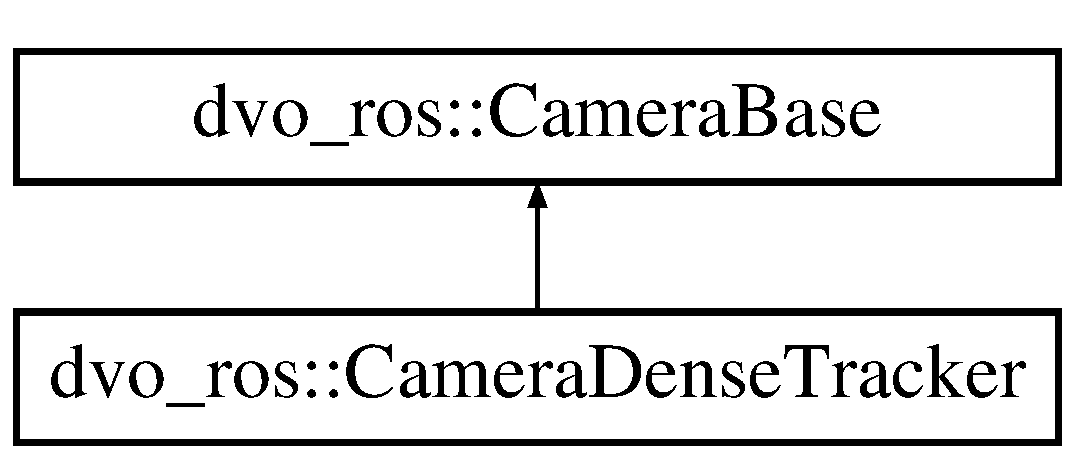
\includegraphics[height=2.000000cm]{classdvo__ros_1_1_camera_base}
\end{center}
\end{figure}
\subsection*{Public Member Functions}
\begin{DoxyCompactItemize}
\item 
\mbox{\hyperlink{classdvo__ros_1_1_camera_base_af3d3ae6aaad83055c752c114b2100104}{Camera\+Base}} (ros\+::\+Node\+Handle \&nh, ros\+::\+Node\+Handle \&nh\+\_\+private)
\item 
virtual \mbox{\hyperlink{classdvo__ros_1_1_camera_base_a022e9f3ea3010cf84bad64fa63f8e1b0}{$\sim$\+Camera\+Base}} ()
\item 
virtual void \mbox{\hyperlink{classdvo__ros_1_1_camera_base_aa8c983ab1bb8383aae1f375ea6808120}{handle\+Images}} (const sensor\+\_\+msgs\+::\+Image\+::\+Const\+Ptr \&rgb\+\_\+image\+\_\+msg, const sensor\+\_\+msgs\+::\+Image\+::\+Const\+Ptr \&depth\+\_\+image\+\_\+msg, const sensor\+\_\+msgs\+::\+Camera\+Info\+::\+Const\+Ptr \&rgb\+\_\+camera\+\_\+info\+\_\+msg, const sensor\+\_\+msgs\+::\+Camera\+Info\+::\+Const\+Ptr \&depth\+\_\+camera\+\_\+info\+\_\+msg)=0
\end{DoxyCompactItemize}
\subsection*{Protected Member Functions}
\begin{DoxyCompactItemize}
\item 
bool \mbox{\hyperlink{classdvo__ros_1_1_camera_base_aca6d7ca1b4238565841cdab72e807765}{is\+Synchronized\+Image\+Stream\+Running}} ()
\item 
void \mbox{\hyperlink{classdvo__ros_1_1_camera_base_a00bdd483ef57eec8a4991c65fef30974}{start\+Synchronized\+Image\+Stream}} ()
\item 
void \mbox{\hyperlink{classdvo__ros_1_1_camera_base_a45929acddbac65ab20b3c0a0b9fb567a}{stop\+Synchronized\+Image\+Stream}} ()
\end{DoxyCompactItemize}
\subsection*{Protected Attributes}
\begin{DoxyCompactItemize}
\item 
ros\+::\+Node\+Handle \mbox{\hyperlink{classdvo__ros_1_1_camera_base_a38fe2cd9f4b4aa6ca843ea317ddf8bad}{nh\+\_\+}}
\item 
ros\+::\+Node\+Handle \mbox{\hyperlink{classdvo__ros_1_1_camera_base_ad8c455ad2a0d51f0cea6072621058b77}{nh\+\_\+private\+\_\+}}
\item 
message\+\_\+filters\+::\+Subscriber$<$ sensor\+\_\+msgs\+::\+Image $>$ \mbox{\hyperlink{classdvo__ros_1_1_camera_base_a38d299b1c046830ef1552a0e4a31d7b2}{rgb\+\_\+image\+\_\+subscriber\+\_\+}}
\item 
message\+\_\+filters\+::\+Subscriber$<$ sensor\+\_\+msgs\+::\+Image $>$ \mbox{\hyperlink{classdvo__ros_1_1_camera_base_a9d2f9d7b4ef5d948d09610d7a518984b}{depth\+\_\+image\+\_\+subscriber\+\_\+}}
\item 
message\+\_\+filters\+::\+Subscriber$<$ sensor\+\_\+msgs\+::\+Camera\+Info $>$ \mbox{\hyperlink{classdvo__ros_1_1_camera_base_a3009d23f7083e4d2aa0c9b52068f96ca}{rgb\+\_\+camera\+\_\+info\+\_\+subscriber\+\_\+}}
\item 
message\+\_\+filters\+::\+Subscriber$<$ sensor\+\_\+msgs\+::\+Camera\+Info $>$ \mbox{\hyperlink{classdvo__ros_1_1_camera_base_aec2df412779aa6ef9643a54a5910424a}{depth\+\_\+camera\+\_\+info\+\_\+subscriber\+\_\+}}
\item 
message\+\_\+filters\+::\+Synchronizer$<$ \mbox{\hyperlink{namespacedvo__ros_ae8c4d74734d4ef3107bf429ef461e553}{R\+G\+B\+D\+With\+Camera\+Info\+Policy}} $>$ \mbox{\hyperlink{classdvo__ros_1_1_camera_base_aac780a822e3a2b6779a2a9598b0b52d2}{synchronizer\+\_\+}}
\end{DoxyCompactItemize}


\subsection{Constructor \& Destructor Documentation}
\mbox{\Hypertarget{classdvo__ros_1_1_camera_base_af3d3ae6aaad83055c752c114b2100104}\label{classdvo__ros_1_1_camera_base_af3d3ae6aaad83055c752c114b2100104}} 
\index{dvo\+\_\+ros\+::\+Camera\+Base@{dvo\+\_\+ros\+::\+Camera\+Base}!Camera\+Base@{Camera\+Base}}
\index{Camera\+Base@{Camera\+Base}!dvo\+\_\+ros\+::\+Camera\+Base@{dvo\+\_\+ros\+::\+Camera\+Base}}
\subsubsection{\texorpdfstring{Camera\+Base()}{CameraBase()}}
{\footnotesize\ttfamily dvo\+\_\+ros\+::\+Camera\+Base\+::\+Camera\+Base (\begin{DoxyParamCaption}\item[{ros\+::\+Node\+Handle \&}]{nh,  }\item[{ros\+::\+Node\+Handle \&}]{nh\+\_\+private }\end{DoxyParamCaption})}

\mbox{\Hypertarget{classdvo__ros_1_1_camera_base_a022e9f3ea3010cf84bad64fa63f8e1b0}\label{classdvo__ros_1_1_camera_base_a022e9f3ea3010cf84bad64fa63f8e1b0}} 
\index{dvo\+\_\+ros\+::\+Camera\+Base@{dvo\+\_\+ros\+::\+Camera\+Base}!````~Camera\+Base@{$\sim$\+Camera\+Base}}
\index{````~Camera\+Base@{$\sim$\+Camera\+Base}!dvo\+\_\+ros\+::\+Camera\+Base@{dvo\+\_\+ros\+::\+Camera\+Base}}
\subsubsection{\texorpdfstring{$\sim$\+Camera\+Base()}{~CameraBase()}}
{\footnotesize\ttfamily dvo\+\_\+ros\+::\+Camera\+Base\+::$\sim$\+Camera\+Base (\begin{DoxyParamCaption}{ }\end{DoxyParamCaption})\hspace{0.3cm}{\ttfamily [virtual]}}



\subsection{Member Function Documentation}
\mbox{\Hypertarget{classdvo__ros_1_1_camera_base_aa8c983ab1bb8383aae1f375ea6808120}\label{classdvo__ros_1_1_camera_base_aa8c983ab1bb8383aae1f375ea6808120}} 
\index{dvo\+\_\+ros\+::\+Camera\+Base@{dvo\+\_\+ros\+::\+Camera\+Base}!handle\+Images@{handle\+Images}}
\index{handle\+Images@{handle\+Images}!dvo\+\_\+ros\+::\+Camera\+Base@{dvo\+\_\+ros\+::\+Camera\+Base}}
\subsubsection{\texorpdfstring{handle\+Images()}{handleImages()}}
{\footnotesize\ttfamily virtual void dvo\+\_\+ros\+::\+Camera\+Base\+::handle\+Images (\begin{DoxyParamCaption}\item[{const sensor\+\_\+msgs\+::\+Image\+::\+Const\+Ptr \&}]{rgb\+\_\+image\+\_\+msg,  }\item[{const sensor\+\_\+msgs\+::\+Image\+::\+Const\+Ptr \&}]{depth\+\_\+image\+\_\+msg,  }\item[{const sensor\+\_\+msgs\+::\+Camera\+Info\+::\+Const\+Ptr \&}]{rgb\+\_\+camera\+\_\+info\+\_\+msg,  }\item[{const sensor\+\_\+msgs\+::\+Camera\+Info\+::\+Const\+Ptr \&}]{depth\+\_\+camera\+\_\+info\+\_\+msg }\end{DoxyParamCaption})\hspace{0.3cm}{\ttfamily [pure virtual]}}



Implemented in \mbox{\hyperlink{classdvo__ros_1_1_camera_dense_tracker_ad1b549d802d0ebc3627603b3f9ef03b4}{dvo\+\_\+ros\+::\+Camera\+Dense\+Tracker}}.

\mbox{\Hypertarget{classdvo__ros_1_1_camera_base_aca6d7ca1b4238565841cdab72e807765}\label{classdvo__ros_1_1_camera_base_aca6d7ca1b4238565841cdab72e807765}} 
\index{dvo\+\_\+ros\+::\+Camera\+Base@{dvo\+\_\+ros\+::\+Camera\+Base}!is\+Synchronized\+Image\+Stream\+Running@{is\+Synchronized\+Image\+Stream\+Running}}
\index{is\+Synchronized\+Image\+Stream\+Running@{is\+Synchronized\+Image\+Stream\+Running}!dvo\+\_\+ros\+::\+Camera\+Base@{dvo\+\_\+ros\+::\+Camera\+Base}}
\subsubsection{\texorpdfstring{is\+Synchronized\+Image\+Stream\+Running()}{isSynchronizedImageStreamRunning()}}
{\footnotesize\ttfamily bool dvo\+\_\+ros\+::\+Camera\+Base\+::is\+Synchronized\+Image\+Stream\+Running (\begin{DoxyParamCaption}{ }\end{DoxyParamCaption})\hspace{0.3cm}{\ttfamily [protected]}}

\mbox{\Hypertarget{classdvo__ros_1_1_camera_base_a00bdd483ef57eec8a4991c65fef30974}\label{classdvo__ros_1_1_camera_base_a00bdd483ef57eec8a4991c65fef30974}} 
\index{dvo\+\_\+ros\+::\+Camera\+Base@{dvo\+\_\+ros\+::\+Camera\+Base}!start\+Synchronized\+Image\+Stream@{start\+Synchronized\+Image\+Stream}}
\index{start\+Synchronized\+Image\+Stream@{start\+Synchronized\+Image\+Stream}!dvo\+\_\+ros\+::\+Camera\+Base@{dvo\+\_\+ros\+::\+Camera\+Base}}
\subsubsection{\texorpdfstring{start\+Synchronized\+Image\+Stream()}{startSynchronizedImageStream()}}
{\footnotesize\ttfamily void dvo\+\_\+ros\+::\+Camera\+Base\+::start\+Synchronized\+Image\+Stream (\begin{DoxyParamCaption}{ }\end{DoxyParamCaption})\hspace{0.3cm}{\ttfamily [protected]}}

\mbox{\Hypertarget{classdvo__ros_1_1_camera_base_a45929acddbac65ab20b3c0a0b9fb567a}\label{classdvo__ros_1_1_camera_base_a45929acddbac65ab20b3c0a0b9fb567a}} 
\index{dvo\+\_\+ros\+::\+Camera\+Base@{dvo\+\_\+ros\+::\+Camera\+Base}!stop\+Synchronized\+Image\+Stream@{stop\+Synchronized\+Image\+Stream}}
\index{stop\+Synchronized\+Image\+Stream@{stop\+Synchronized\+Image\+Stream}!dvo\+\_\+ros\+::\+Camera\+Base@{dvo\+\_\+ros\+::\+Camera\+Base}}
\subsubsection{\texorpdfstring{stop\+Synchronized\+Image\+Stream()}{stopSynchronizedImageStream()}}
{\footnotesize\ttfamily void dvo\+\_\+ros\+::\+Camera\+Base\+::stop\+Synchronized\+Image\+Stream (\begin{DoxyParamCaption}{ }\end{DoxyParamCaption})\hspace{0.3cm}{\ttfamily [protected]}}



\subsection{Member Data Documentation}
\mbox{\Hypertarget{classdvo__ros_1_1_camera_base_aec2df412779aa6ef9643a54a5910424a}\label{classdvo__ros_1_1_camera_base_aec2df412779aa6ef9643a54a5910424a}} 
\index{dvo\+\_\+ros\+::\+Camera\+Base@{dvo\+\_\+ros\+::\+Camera\+Base}!depth\+\_\+camera\+\_\+info\+\_\+subscriber\+\_\+@{depth\+\_\+camera\+\_\+info\+\_\+subscriber\+\_\+}}
\index{depth\+\_\+camera\+\_\+info\+\_\+subscriber\+\_\+@{depth\+\_\+camera\+\_\+info\+\_\+subscriber\+\_\+}!dvo\+\_\+ros\+::\+Camera\+Base@{dvo\+\_\+ros\+::\+Camera\+Base}}
\subsubsection{\texorpdfstring{depth\+\_\+camera\+\_\+info\+\_\+subscriber\+\_\+}{depth\_camera\_info\_subscriber\_}}
{\footnotesize\ttfamily message\+\_\+filters\+::\+Subscriber$<$sensor\+\_\+msgs\+::\+Camera\+Info$>$ dvo\+\_\+ros\+::\+Camera\+Base\+::depth\+\_\+camera\+\_\+info\+\_\+subscriber\+\_\+\hspace{0.3cm}{\ttfamily [protected]}}

\mbox{\Hypertarget{classdvo__ros_1_1_camera_base_a9d2f9d7b4ef5d948d09610d7a518984b}\label{classdvo__ros_1_1_camera_base_a9d2f9d7b4ef5d948d09610d7a518984b}} 
\index{dvo\+\_\+ros\+::\+Camera\+Base@{dvo\+\_\+ros\+::\+Camera\+Base}!depth\+\_\+image\+\_\+subscriber\+\_\+@{depth\+\_\+image\+\_\+subscriber\+\_\+}}
\index{depth\+\_\+image\+\_\+subscriber\+\_\+@{depth\+\_\+image\+\_\+subscriber\+\_\+}!dvo\+\_\+ros\+::\+Camera\+Base@{dvo\+\_\+ros\+::\+Camera\+Base}}
\subsubsection{\texorpdfstring{depth\+\_\+image\+\_\+subscriber\+\_\+}{depth\_image\_subscriber\_}}
{\footnotesize\ttfamily message\+\_\+filters\+::\+Subscriber$<$sensor\+\_\+msgs\+::\+Image$>$ dvo\+\_\+ros\+::\+Camera\+Base\+::depth\+\_\+image\+\_\+subscriber\+\_\+\hspace{0.3cm}{\ttfamily [protected]}}

\mbox{\Hypertarget{classdvo__ros_1_1_camera_base_a38fe2cd9f4b4aa6ca843ea317ddf8bad}\label{classdvo__ros_1_1_camera_base_a38fe2cd9f4b4aa6ca843ea317ddf8bad}} 
\index{dvo\+\_\+ros\+::\+Camera\+Base@{dvo\+\_\+ros\+::\+Camera\+Base}!nh\+\_\+@{nh\+\_\+}}
\index{nh\+\_\+@{nh\+\_\+}!dvo\+\_\+ros\+::\+Camera\+Base@{dvo\+\_\+ros\+::\+Camera\+Base}}
\subsubsection{\texorpdfstring{nh\+\_\+}{nh\_}}
{\footnotesize\ttfamily ros\+::\+Node\+Handle dvo\+\_\+ros\+::\+Camera\+Base\+::nh\+\_\+\hspace{0.3cm}{\ttfamily [protected]}}

\mbox{\Hypertarget{classdvo__ros_1_1_camera_base_ad8c455ad2a0d51f0cea6072621058b77}\label{classdvo__ros_1_1_camera_base_ad8c455ad2a0d51f0cea6072621058b77}} 
\index{dvo\+\_\+ros\+::\+Camera\+Base@{dvo\+\_\+ros\+::\+Camera\+Base}!nh\+\_\+private\+\_\+@{nh\+\_\+private\+\_\+}}
\index{nh\+\_\+private\+\_\+@{nh\+\_\+private\+\_\+}!dvo\+\_\+ros\+::\+Camera\+Base@{dvo\+\_\+ros\+::\+Camera\+Base}}
\subsubsection{\texorpdfstring{nh\+\_\+private\+\_\+}{nh\_private\_}}
{\footnotesize\ttfamily ros\+::\+Node\+Handle dvo\+\_\+ros\+::\+Camera\+Base\+::nh\+\_\+private\+\_\+\hspace{0.3cm}{\ttfamily [protected]}}

\mbox{\Hypertarget{classdvo__ros_1_1_camera_base_a3009d23f7083e4d2aa0c9b52068f96ca}\label{classdvo__ros_1_1_camera_base_a3009d23f7083e4d2aa0c9b52068f96ca}} 
\index{dvo\+\_\+ros\+::\+Camera\+Base@{dvo\+\_\+ros\+::\+Camera\+Base}!rgb\+\_\+camera\+\_\+info\+\_\+subscriber\+\_\+@{rgb\+\_\+camera\+\_\+info\+\_\+subscriber\+\_\+}}
\index{rgb\+\_\+camera\+\_\+info\+\_\+subscriber\+\_\+@{rgb\+\_\+camera\+\_\+info\+\_\+subscriber\+\_\+}!dvo\+\_\+ros\+::\+Camera\+Base@{dvo\+\_\+ros\+::\+Camera\+Base}}
\subsubsection{\texorpdfstring{rgb\+\_\+camera\+\_\+info\+\_\+subscriber\+\_\+}{rgb\_camera\_info\_subscriber\_}}
{\footnotesize\ttfamily message\+\_\+filters\+::\+Subscriber$<$sensor\+\_\+msgs\+::\+Camera\+Info$>$ dvo\+\_\+ros\+::\+Camera\+Base\+::rgb\+\_\+camera\+\_\+info\+\_\+subscriber\+\_\+\hspace{0.3cm}{\ttfamily [protected]}}

\mbox{\Hypertarget{classdvo__ros_1_1_camera_base_a38d299b1c046830ef1552a0e4a31d7b2}\label{classdvo__ros_1_1_camera_base_a38d299b1c046830ef1552a0e4a31d7b2}} 
\index{dvo\+\_\+ros\+::\+Camera\+Base@{dvo\+\_\+ros\+::\+Camera\+Base}!rgb\+\_\+image\+\_\+subscriber\+\_\+@{rgb\+\_\+image\+\_\+subscriber\+\_\+}}
\index{rgb\+\_\+image\+\_\+subscriber\+\_\+@{rgb\+\_\+image\+\_\+subscriber\+\_\+}!dvo\+\_\+ros\+::\+Camera\+Base@{dvo\+\_\+ros\+::\+Camera\+Base}}
\subsubsection{\texorpdfstring{rgb\+\_\+image\+\_\+subscriber\+\_\+}{rgb\_image\_subscriber\_}}
{\footnotesize\ttfamily message\+\_\+filters\+::\+Subscriber$<$sensor\+\_\+msgs\+::\+Image$>$ dvo\+\_\+ros\+::\+Camera\+Base\+::rgb\+\_\+image\+\_\+subscriber\+\_\+\hspace{0.3cm}{\ttfamily [protected]}}

\mbox{\Hypertarget{classdvo__ros_1_1_camera_base_aac780a822e3a2b6779a2a9598b0b52d2}\label{classdvo__ros_1_1_camera_base_aac780a822e3a2b6779a2a9598b0b52d2}} 
\index{dvo\+\_\+ros\+::\+Camera\+Base@{dvo\+\_\+ros\+::\+Camera\+Base}!synchronizer\+\_\+@{synchronizer\+\_\+}}
\index{synchronizer\+\_\+@{synchronizer\+\_\+}!dvo\+\_\+ros\+::\+Camera\+Base@{dvo\+\_\+ros\+::\+Camera\+Base}}
\subsubsection{\texorpdfstring{synchronizer\+\_\+}{synchronizer\_}}
{\footnotesize\ttfamily message\+\_\+filters\+::\+Synchronizer$<$\mbox{\hyperlink{namespacedvo__ros_ae8c4d74734d4ef3107bf429ef461e553}{R\+G\+B\+D\+With\+Camera\+Info\+Policy}}$>$ dvo\+\_\+ros\+::\+Camera\+Base\+::synchronizer\+\_\+\hspace{0.3cm}{\ttfamily [protected]}}



The documentation for this class was generated from the following files\+:\begin{DoxyCompactItemize}
\item 
dvo\+\_\+ros/include/dvo\+\_\+ros/\mbox{\hyperlink{camera__base_8h}{camera\+\_\+base.\+h}}\item 
dvo\+\_\+ros/src/\mbox{\hyperlink{camera__base_8cpp}{camera\+\_\+base.\+cpp}}\end{DoxyCompactItemize}

\hypertarget{classdvo__ros_1_1_camera_dense_tracker}{}\section{dvo\+\_\+ros\+:\+:Camera\+Dense\+Tracker Class Reference}
\label{classdvo__ros_1_1_camera_dense_tracker}\index{dvo\+\_\+ros\+::\+Camera\+Dense\+Tracker@{dvo\+\_\+ros\+::\+Camera\+Dense\+Tracker}}


{\ttfamily \#include $<$camera\+\_\+dense\+\_\+tracking.\+h$>$}

Inheritance diagram for dvo\+\_\+ros\+:\+:Camera\+Dense\+Tracker\+:\begin{figure}[H]
\begin{center}
\leavevmode
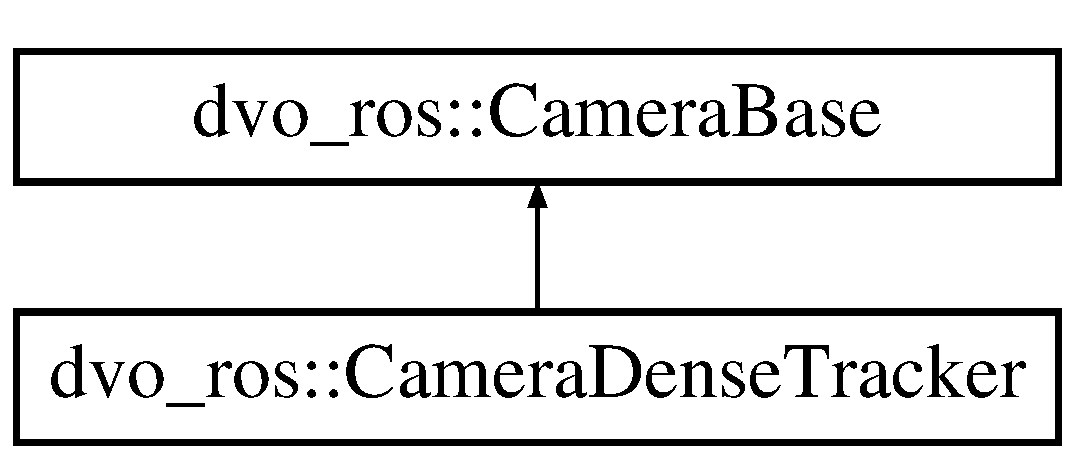
\includegraphics[height=2.000000cm]{classdvo__ros_1_1_camera_dense_tracker}
\end{center}
\end{figure}
\subsection*{Public Member Functions}
\begin{DoxyCompactItemize}
\item 
\mbox{\hyperlink{classdvo__ros_1_1_camera_dense_tracker_a85604036a34ea68a29dc80a3ea782ee7}{Camera\+Dense\+Tracker}} (ros\+::\+Node\+Handle \&nh, ros\+::\+Node\+Handle \&nh\+\_\+private)
\item 
virtual \mbox{\hyperlink{classdvo__ros_1_1_camera_dense_tracker_ae8ab4b242a3149461825976d4d310aaf}{$\sim$\+Camera\+Dense\+Tracker}} ()
\item 
virtual void \mbox{\hyperlink{classdvo__ros_1_1_camera_dense_tracker_ad1b549d802d0ebc3627603b3f9ef03b4}{handle\+Images}} (const sensor\+\_\+msgs\+::\+Image\+::\+Const\+Ptr \&rgb\+\_\+image\+\_\+msg, const sensor\+\_\+msgs\+::\+Image\+::\+Const\+Ptr \&depth\+\_\+image\+\_\+msg, const sensor\+\_\+msgs\+::\+Camera\+Info\+::\+Const\+Ptr \&rgb\+\_\+camera\+\_\+info\+\_\+msg, const sensor\+\_\+msgs\+::\+Camera\+Info\+::\+Const\+Ptr \&depth\+\_\+camera\+\_\+info\+\_\+msg)
\item 
void \mbox{\hyperlink{classdvo__ros_1_1_camera_dense_tracker_a385c851351c4ab22240409d2d340344f}{handle\+Pose}} (const geometry\+\_\+msgs\+::\+Pose\+With\+Covariance\+Stamped\+Const\+Ptr \&pose)
\item 
void \mbox{\hyperlink{classdvo__ros_1_1_camera_dense_tracker_a7fce574520d9ca9056636506db504912}{handle\+Config}} (dvo\+\_\+ros\+::\+Camera\+Dense\+Tracker\+Config \&config, uint32\+\_\+t level)
\end{DoxyCompactItemize}
\subsection*{Additional Inherited Members}


\subsection{Constructor \& Destructor Documentation}
\mbox{\Hypertarget{classdvo__ros_1_1_camera_dense_tracker_a85604036a34ea68a29dc80a3ea782ee7}\label{classdvo__ros_1_1_camera_dense_tracker_a85604036a34ea68a29dc80a3ea782ee7}} 
\index{dvo\+\_\+ros\+::\+Camera\+Dense\+Tracker@{dvo\+\_\+ros\+::\+Camera\+Dense\+Tracker}!Camera\+Dense\+Tracker@{Camera\+Dense\+Tracker}}
\index{Camera\+Dense\+Tracker@{Camera\+Dense\+Tracker}!dvo\+\_\+ros\+::\+Camera\+Dense\+Tracker@{dvo\+\_\+ros\+::\+Camera\+Dense\+Tracker}}
\subsubsection{\texorpdfstring{Camera\+Dense\+Tracker()}{CameraDenseTracker()}}
{\footnotesize\ttfamily dvo\+\_\+ros\+::\+Camera\+Dense\+Tracker\+::\+Camera\+Dense\+Tracker (\begin{DoxyParamCaption}\item[{ros\+::\+Node\+Handle \&}]{nh,  }\item[{ros\+::\+Node\+Handle \&}]{nh\+\_\+private }\end{DoxyParamCaption})}

\mbox{\Hypertarget{classdvo__ros_1_1_camera_dense_tracker_ae8ab4b242a3149461825976d4d310aaf}\label{classdvo__ros_1_1_camera_dense_tracker_ae8ab4b242a3149461825976d4d310aaf}} 
\index{dvo\+\_\+ros\+::\+Camera\+Dense\+Tracker@{dvo\+\_\+ros\+::\+Camera\+Dense\+Tracker}!````~Camera\+Dense\+Tracker@{$\sim$\+Camera\+Dense\+Tracker}}
\index{````~Camera\+Dense\+Tracker@{$\sim$\+Camera\+Dense\+Tracker}!dvo\+\_\+ros\+::\+Camera\+Dense\+Tracker@{dvo\+\_\+ros\+::\+Camera\+Dense\+Tracker}}
\subsubsection{\texorpdfstring{$\sim$\+Camera\+Dense\+Tracker()}{~CameraDenseTracker()}}
{\footnotesize\ttfamily dvo\+\_\+ros\+::\+Camera\+Dense\+Tracker\+::$\sim$\+Camera\+Dense\+Tracker (\begin{DoxyParamCaption}{ }\end{DoxyParamCaption})\hspace{0.3cm}{\ttfamily [virtual]}}



\subsection{Member Function Documentation}
\mbox{\Hypertarget{classdvo__ros_1_1_camera_dense_tracker_a7fce574520d9ca9056636506db504912}\label{classdvo__ros_1_1_camera_dense_tracker_a7fce574520d9ca9056636506db504912}} 
\index{dvo\+\_\+ros\+::\+Camera\+Dense\+Tracker@{dvo\+\_\+ros\+::\+Camera\+Dense\+Tracker}!handle\+Config@{handle\+Config}}
\index{handle\+Config@{handle\+Config}!dvo\+\_\+ros\+::\+Camera\+Dense\+Tracker@{dvo\+\_\+ros\+::\+Camera\+Dense\+Tracker}}
\subsubsection{\texorpdfstring{handle\+Config()}{handleConfig()}}
{\footnotesize\ttfamily void dvo\+\_\+ros\+::\+Camera\+Dense\+Tracker\+::handle\+Config (\begin{DoxyParamCaption}\item[{dvo\+\_\+ros\+::\+Camera\+Dense\+Tracker\+Config \&}]{config,  }\item[{uint32\+\_\+t}]{level }\end{DoxyParamCaption})}

dynamic reconfigure the tracker node. \mbox{\Hypertarget{classdvo__ros_1_1_camera_dense_tracker_ad1b549d802d0ebc3627603b3f9ef03b4}\label{classdvo__ros_1_1_camera_dense_tracker_ad1b549d802d0ebc3627603b3f9ef03b4}} 
\index{dvo\+\_\+ros\+::\+Camera\+Dense\+Tracker@{dvo\+\_\+ros\+::\+Camera\+Dense\+Tracker}!handle\+Images@{handle\+Images}}
\index{handle\+Images@{handle\+Images}!dvo\+\_\+ros\+::\+Camera\+Dense\+Tracker@{dvo\+\_\+ros\+::\+Camera\+Dense\+Tracker}}
\subsubsection{\texorpdfstring{handle\+Images()}{handleImages()}}
{\footnotesize\ttfamily void dvo\+\_\+ros\+::\+Camera\+Dense\+Tracker\+::handle\+Images (\begin{DoxyParamCaption}\item[{const sensor\+\_\+msgs\+::\+Image\+::\+Const\+Ptr \&}]{rgb\+\_\+image\+\_\+msg,  }\item[{const sensor\+\_\+msgs\+::\+Image\+::\+Const\+Ptr \&}]{depth\+\_\+image\+\_\+msg,  }\item[{const sensor\+\_\+msgs\+::\+Camera\+Info\+::\+Const\+Ptr \&}]{rgb\+\_\+camera\+\_\+info\+\_\+msg,  }\item[{const sensor\+\_\+msgs\+::\+Camera\+Info\+::\+Const\+Ptr \&}]{depth\+\_\+camera\+\_\+info\+\_\+msg }\end{DoxyParamCaption})\hspace{0.3cm}{\ttfamily [virtual]}}

Important\+: The framework convert R\+GB image to Intensity, C\+V\+\_\+32F, depth image, reference pair is swapped by the current pair and current pair is reset by the new Rgbd\+Image\+Pyramid generated by the newly recieved intensity and depth image. then call the tracker-\/$>$match() function . 

Implements \mbox{\hyperlink{classdvo__ros_1_1_camera_base_aa8c983ab1bb8383aae1f375ea6808120}{dvo\+\_\+ros\+::\+Camera\+Base}}.

\mbox{\Hypertarget{classdvo__ros_1_1_camera_dense_tracker_a385c851351c4ab22240409d2d340344f}\label{classdvo__ros_1_1_camera_dense_tracker_a385c851351c4ab22240409d2d340344f}} 
\index{dvo\+\_\+ros\+::\+Camera\+Dense\+Tracker@{dvo\+\_\+ros\+::\+Camera\+Dense\+Tracker}!handle\+Pose@{handle\+Pose}}
\index{handle\+Pose@{handle\+Pose}!dvo\+\_\+ros\+::\+Camera\+Dense\+Tracker@{dvo\+\_\+ros\+::\+Camera\+Dense\+Tracker}}
\subsubsection{\texorpdfstring{handle\+Pose()}{handlePose()}}
{\footnotesize\ttfamily void dvo\+\_\+ros\+::\+Camera\+Dense\+Tracker\+::handle\+Pose (\begin{DoxyParamCaption}\item[{const geometry\+\_\+msgs\+::\+Pose\+With\+Covariance\+Stamped\+Const\+Ptr \&}]{pose }\end{DoxyParamCaption})}

Just publish the pose. 

The documentation for this class was generated from the following files\+:\begin{DoxyCompactItemize}
\item 
dvo\+\_\+ros/include/dvo\+\_\+ros/\mbox{\hyperlink{camera__dense__tracking_8h}{camera\+\_\+dense\+\_\+tracking.\+h}}\item 
dvo\+\_\+ros/src/\mbox{\hyperlink{camera__dense__tracking_8cpp}{camera\+\_\+dense\+\_\+tracking.\+cpp}}\end{DoxyCompactItemize}

\hypertarget{classdvo__ros_1_1_camera_tracker_nodelet}{}\section{dvo\+\_\+ros\+:\+:Camera\+Tracker\+Nodelet Class Reference}
\label{classdvo__ros_1_1_camera_tracker_nodelet}\index{dvo\+\_\+ros\+::\+Camera\+Tracker\+Nodelet@{dvo\+\_\+ros\+::\+Camera\+Tracker\+Nodelet}}


{\ttfamily \#include $<$camera\+\_\+tracker\+\_\+nodelet.\+h$>$}

Inheritance diagram for dvo\+\_\+ros\+:\+:Camera\+Tracker\+Nodelet\+:\begin{figure}[H]
\begin{center}
\leavevmode
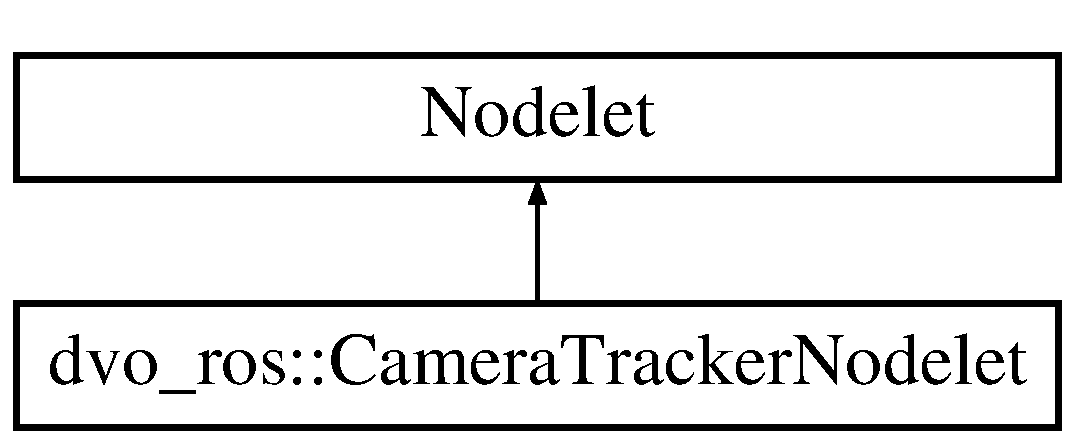
\includegraphics[height=2.000000cm]{classdvo__ros_1_1_camera_tracker_nodelet}
\end{center}
\end{figure}
\subsection*{Public Member Functions}
\begin{DoxyCompactItemize}
\item 
\mbox{\hyperlink{classdvo__ros_1_1_camera_tracker_nodelet_a7320ee469172ee85ebbdeb470cc11d15}{Camera\+Tracker\+Nodelet}} ()
\item 
virtual \mbox{\hyperlink{classdvo__ros_1_1_camera_tracker_nodelet_a8189fa86e3b8bfbd2397b47b4dfa17d7}{$\sim$\+Camera\+Tracker\+Nodelet}} ()
\item 
virtual void \mbox{\hyperlink{classdvo__ros_1_1_camera_tracker_nodelet_a62ab6e4908aa2547c60e0247bb4cb2e3}{on\+Init}} ()
\end{DoxyCompactItemize}


\subsection{Constructor \& Destructor Documentation}
\mbox{\Hypertarget{classdvo__ros_1_1_camera_tracker_nodelet_a7320ee469172ee85ebbdeb470cc11d15}\label{classdvo__ros_1_1_camera_tracker_nodelet_a7320ee469172ee85ebbdeb470cc11d15}} 
\index{dvo\+\_\+ros\+::\+Camera\+Tracker\+Nodelet@{dvo\+\_\+ros\+::\+Camera\+Tracker\+Nodelet}!Camera\+Tracker\+Nodelet@{Camera\+Tracker\+Nodelet}}
\index{Camera\+Tracker\+Nodelet@{Camera\+Tracker\+Nodelet}!dvo\+\_\+ros\+::\+Camera\+Tracker\+Nodelet@{dvo\+\_\+ros\+::\+Camera\+Tracker\+Nodelet}}
\subsubsection{\texorpdfstring{Camera\+Tracker\+Nodelet()}{CameraTrackerNodelet()}}
{\footnotesize\ttfamily dvo\+\_\+ros\+::\+Camera\+Tracker\+Nodelet\+::\+Camera\+Tracker\+Nodelet (\begin{DoxyParamCaption}{ }\end{DoxyParamCaption})}

\mbox{\Hypertarget{classdvo__ros_1_1_camera_tracker_nodelet_a8189fa86e3b8bfbd2397b47b4dfa17d7}\label{classdvo__ros_1_1_camera_tracker_nodelet_a8189fa86e3b8bfbd2397b47b4dfa17d7}} 
\index{dvo\+\_\+ros\+::\+Camera\+Tracker\+Nodelet@{dvo\+\_\+ros\+::\+Camera\+Tracker\+Nodelet}!````~Camera\+Tracker\+Nodelet@{$\sim$\+Camera\+Tracker\+Nodelet}}
\index{````~Camera\+Tracker\+Nodelet@{$\sim$\+Camera\+Tracker\+Nodelet}!dvo\+\_\+ros\+::\+Camera\+Tracker\+Nodelet@{dvo\+\_\+ros\+::\+Camera\+Tracker\+Nodelet}}
\subsubsection{\texorpdfstring{$\sim$\+Camera\+Tracker\+Nodelet()}{~CameraTrackerNodelet()}}
{\footnotesize\ttfamily dvo\+\_\+ros\+::\+Camera\+Tracker\+Nodelet\+::$\sim$\+Camera\+Tracker\+Nodelet (\begin{DoxyParamCaption}{ }\end{DoxyParamCaption})\hspace{0.3cm}{\ttfamily [virtual]}}



\subsection{Member Function Documentation}
\mbox{\Hypertarget{classdvo__ros_1_1_camera_tracker_nodelet_a62ab6e4908aa2547c60e0247bb4cb2e3}\label{classdvo__ros_1_1_camera_tracker_nodelet_a62ab6e4908aa2547c60e0247bb4cb2e3}} 
\index{dvo\+\_\+ros\+::\+Camera\+Tracker\+Nodelet@{dvo\+\_\+ros\+::\+Camera\+Tracker\+Nodelet}!on\+Init@{on\+Init}}
\index{on\+Init@{on\+Init}!dvo\+\_\+ros\+::\+Camera\+Tracker\+Nodelet@{dvo\+\_\+ros\+::\+Camera\+Tracker\+Nodelet}}
\subsubsection{\texorpdfstring{on\+Init()}{onInit()}}
{\footnotesize\ttfamily void dvo\+\_\+ros\+::\+Camera\+Tracker\+Nodelet\+::on\+Init (\begin{DoxyParamCaption}{ }\end{DoxyParamCaption})\hspace{0.3cm}{\ttfamily [virtual]}}



The documentation for this class was generated from the following files\+:\begin{DoxyCompactItemize}
\item 
dvo\+\_\+ros/include/dvo\+\_\+ros/\mbox{\hyperlink{camera__tracker__nodelet_8h}{camera\+\_\+tracker\+\_\+nodelet.\+h}}\item 
dvo\+\_\+ros/src/\mbox{\hyperlink{camera__tracker__nodelet_8cpp}{camera\+\_\+tracker\+\_\+nodelet.\+cpp}}\end{DoxyCompactItemize}

\hypertarget{classdvo_1_1visualization_1_1_camera_trajectory_visualizer_interface}{}\section{dvo\+:\+:visualization\+:\+:Camera\+Trajectory\+Visualizer\+Interface Class Reference}
\label{classdvo_1_1visualization_1_1_camera_trajectory_visualizer_interface}\index{dvo\+::visualization\+::\+Camera\+Trajectory\+Visualizer\+Interface@{dvo\+::visualization\+::\+Camera\+Trajectory\+Visualizer\+Interface}}


{\ttfamily \#include $<$camera\+\_\+trajectory\+\_\+visualizer.\+h$>$}

Inheritance diagram for dvo\+:\+:visualization\+:\+:Camera\+Trajectory\+Visualizer\+Interface\+:\begin{figure}[H]
\begin{center}
\leavevmode
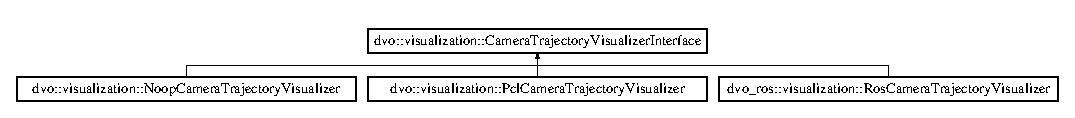
\includegraphics[height=1.131313cm]{classdvo_1_1visualization_1_1_camera_trajectory_visualizer_interface}
\end{center}
\end{figure}
\subsection*{Public Member Functions}
\begin{DoxyCompactItemize}
\item 
virtual \mbox{\hyperlink{classdvo_1_1visualization_1_1_camera_trajectory_visualizer_interface_ac0b5599dd9994a0283eaaa227d609bfd}{$\sim$\+Camera\+Trajectory\+Visualizer\+Interface}} ()
\item 
virtual \mbox{\hyperlink{classdvo_1_1visualization_1_1_camera_visualizer_a473ebecc62e1d4edba21027d858789a2}{Camera\+Visualizer\+::\+Ptr}} \mbox{\hyperlink{classdvo_1_1visualization_1_1_camera_trajectory_visualizer_interface_a4d43cd43f26bd880eb07e8ee37a7154a}{camera}} (std\+::string name)=0
\item 
virtual \mbox{\hyperlink{classdvo_1_1visualization_1_1_trajectory_visualizer_aac33ef5979fe64ee33409f1afa977fd3}{Trajectory\+Visualizer\+::\+Ptr}} \mbox{\hyperlink{classdvo_1_1visualization_1_1_camera_trajectory_visualizer_interface_ac658e841335e51c50325267de10e64b3}{trajectory}} (std\+::string name)=0
\item 
virtual void \mbox{\hyperlink{classdvo_1_1visualization_1_1_camera_trajectory_visualizer_interface_abcc7ddffc30b41eb9112c386f3e41aa7}{reset}} ()=0
\item 
virtual bool \mbox{\hyperlink{classdvo_1_1visualization_1_1_camera_trajectory_visualizer_interface_aa034546bfbdfa55855c56ab21df41b8e}{native}} (void $\ast$\&native\+\_\+visualizer)
\end{DoxyCompactItemize}


\subsection{Constructor \& Destructor Documentation}
\mbox{\Hypertarget{classdvo_1_1visualization_1_1_camera_trajectory_visualizer_interface_ac0b5599dd9994a0283eaaa227d609bfd}\label{classdvo_1_1visualization_1_1_camera_trajectory_visualizer_interface_ac0b5599dd9994a0283eaaa227d609bfd}} 
\index{dvo\+::visualization\+::\+Camera\+Trajectory\+Visualizer\+Interface@{dvo\+::visualization\+::\+Camera\+Trajectory\+Visualizer\+Interface}!````~Camera\+Trajectory\+Visualizer\+Interface@{$\sim$\+Camera\+Trajectory\+Visualizer\+Interface}}
\index{````~Camera\+Trajectory\+Visualizer\+Interface@{$\sim$\+Camera\+Trajectory\+Visualizer\+Interface}!dvo\+::visualization\+::\+Camera\+Trajectory\+Visualizer\+Interface@{dvo\+::visualization\+::\+Camera\+Trajectory\+Visualizer\+Interface}}
\subsubsection{\texorpdfstring{$\sim$\+Camera\+Trajectory\+Visualizer\+Interface()}{~CameraTrajectoryVisualizerInterface()}}
{\footnotesize\ttfamily virtual dvo\+::visualization\+::\+Camera\+Trajectory\+Visualizer\+Interface\+::$\sim$\+Camera\+Trajectory\+Visualizer\+Interface (\begin{DoxyParamCaption}{ }\end{DoxyParamCaption})\hspace{0.3cm}{\ttfamily [inline]}, {\ttfamily [virtual]}}



\subsection{Member Function Documentation}
\mbox{\Hypertarget{classdvo_1_1visualization_1_1_camera_trajectory_visualizer_interface_a4d43cd43f26bd880eb07e8ee37a7154a}\label{classdvo_1_1visualization_1_1_camera_trajectory_visualizer_interface_a4d43cd43f26bd880eb07e8ee37a7154a}} 
\index{dvo\+::visualization\+::\+Camera\+Trajectory\+Visualizer\+Interface@{dvo\+::visualization\+::\+Camera\+Trajectory\+Visualizer\+Interface}!camera@{camera}}
\index{camera@{camera}!dvo\+::visualization\+::\+Camera\+Trajectory\+Visualizer\+Interface@{dvo\+::visualization\+::\+Camera\+Trajectory\+Visualizer\+Interface}}
\subsubsection{\texorpdfstring{camera()}{camera()}}
{\footnotesize\ttfamily virtual \mbox{\hyperlink{classdvo_1_1visualization_1_1_camera_visualizer_a473ebecc62e1d4edba21027d858789a2}{Camera\+Visualizer\+::\+Ptr}} dvo\+::visualization\+::\+Camera\+Trajectory\+Visualizer\+Interface\+::camera (\begin{DoxyParamCaption}\item[{std\+::string}]{name }\end{DoxyParamCaption})\hspace{0.3cm}{\ttfamily [pure virtual]}}



Implemented in \mbox{\hyperlink{classdvo_1_1visualization_1_1_noop_camera_trajectory_visualizer_afaf7c129a6112015c81a2e25d0002966}{dvo\+::visualization\+::\+Noop\+Camera\+Trajectory\+Visualizer}}, \mbox{\hyperlink{classdvo_1_1visualization_1_1_pcl_camera_trajectory_visualizer_af808188bb664cdaac442f79fe67b40a6}{dvo\+::visualization\+::\+Pcl\+Camera\+Trajectory\+Visualizer}}, and \mbox{\hyperlink{classdvo__ros_1_1visualization_1_1_ros_camera_trajectory_visualizer_a9595c8a8bfceffb2da725b462569404c}{dvo\+\_\+ros\+::visualization\+::\+Ros\+Camera\+Trajectory\+Visualizer}}.

\mbox{\Hypertarget{classdvo_1_1visualization_1_1_camera_trajectory_visualizer_interface_aa034546bfbdfa55855c56ab21df41b8e}\label{classdvo_1_1visualization_1_1_camera_trajectory_visualizer_interface_aa034546bfbdfa55855c56ab21df41b8e}} 
\index{dvo\+::visualization\+::\+Camera\+Trajectory\+Visualizer\+Interface@{dvo\+::visualization\+::\+Camera\+Trajectory\+Visualizer\+Interface}!native@{native}}
\index{native@{native}!dvo\+::visualization\+::\+Camera\+Trajectory\+Visualizer\+Interface@{dvo\+::visualization\+::\+Camera\+Trajectory\+Visualizer\+Interface}}
\subsubsection{\texorpdfstring{native()}{native()}}
{\footnotesize\ttfamily virtual bool dvo\+::visualization\+::\+Camera\+Trajectory\+Visualizer\+Interface\+::native (\begin{DoxyParamCaption}\item[{void $\ast$\&}]{native\+\_\+visualizer }\end{DoxyParamCaption})\hspace{0.3cm}{\ttfamily [inline]}, {\ttfamily [virtual]}}



Reimplemented in \mbox{\hyperlink{classdvo__ros_1_1visualization_1_1_ros_camera_trajectory_visualizer_a2e5c80d7dc8308ac038be2e4b71f4e25}{dvo\+\_\+ros\+::visualization\+::\+Ros\+Camera\+Trajectory\+Visualizer}}.

\mbox{\Hypertarget{classdvo_1_1visualization_1_1_camera_trajectory_visualizer_interface_abcc7ddffc30b41eb9112c386f3e41aa7}\label{classdvo_1_1visualization_1_1_camera_trajectory_visualizer_interface_abcc7ddffc30b41eb9112c386f3e41aa7}} 
\index{dvo\+::visualization\+::\+Camera\+Trajectory\+Visualizer\+Interface@{dvo\+::visualization\+::\+Camera\+Trajectory\+Visualizer\+Interface}!reset@{reset}}
\index{reset@{reset}!dvo\+::visualization\+::\+Camera\+Trajectory\+Visualizer\+Interface@{dvo\+::visualization\+::\+Camera\+Trajectory\+Visualizer\+Interface}}
\subsubsection{\texorpdfstring{reset()}{reset()}}
{\footnotesize\ttfamily virtual void dvo\+::visualization\+::\+Camera\+Trajectory\+Visualizer\+Interface\+::reset (\begin{DoxyParamCaption}{ }\end{DoxyParamCaption})\hspace{0.3cm}{\ttfamily [pure virtual]}}



Implemented in \mbox{\hyperlink{classdvo_1_1visualization_1_1_noop_camera_trajectory_visualizer_afa3b5e4aff0306755ca3b53ef70008c4}{dvo\+::visualization\+::\+Noop\+Camera\+Trajectory\+Visualizer}}, \mbox{\hyperlink{classdvo_1_1visualization_1_1_pcl_camera_trajectory_visualizer_a1dd833071b1343a97c0366d3ced0799b}{dvo\+::visualization\+::\+Pcl\+Camera\+Trajectory\+Visualizer}}, and \mbox{\hyperlink{classdvo__ros_1_1visualization_1_1_ros_camera_trajectory_visualizer_a1900ce8a2c17014fef1a4375d8fd6e92}{dvo\+\_\+ros\+::visualization\+::\+Ros\+Camera\+Trajectory\+Visualizer}}.

\mbox{\Hypertarget{classdvo_1_1visualization_1_1_camera_trajectory_visualizer_interface_ac658e841335e51c50325267de10e64b3}\label{classdvo_1_1visualization_1_1_camera_trajectory_visualizer_interface_ac658e841335e51c50325267de10e64b3}} 
\index{dvo\+::visualization\+::\+Camera\+Trajectory\+Visualizer\+Interface@{dvo\+::visualization\+::\+Camera\+Trajectory\+Visualizer\+Interface}!trajectory@{trajectory}}
\index{trajectory@{trajectory}!dvo\+::visualization\+::\+Camera\+Trajectory\+Visualizer\+Interface@{dvo\+::visualization\+::\+Camera\+Trajectory\+Visualizer\+Interface}}
\subsubsection{\texorpdfstring{trajectory()}{trajectory()}}
{\footnotesize\ttfamily virtual \mbox{\hyperlink{classdvo_1_1visualization_1_1_trajectory_visualizer_aac33ef5979fe64ee33409f1afa977fd3}{Trajectory\+Visualizer\+::\+Ptr}} dvo\+::visualization\+::\+Camera\+Trajectory\+Visualizer\+Interface\+::trajectory (\begin{DoxyParamCaption}\item[{std\+::string}]{name }\end{DoxyParamCaption})\hspace{0.3cm}{\ttfamily [pure virtual]}}



Implemented in \mbox{\hyperlink{classdvo_1_1visualization_1_1_noop_camera_trajectory_visualizer_a73cd3c7ed8a3817c5f6d480d97aa24c5}{dvo\+::visualization\+::\+Noop\+Camera\+Trajectory\+Visualizer}}, \mbox{\hyperlink{classdvo_1_1visualization_1_1_pcl_camera_trajectory_visualizer_ad0ea0d8feefef54cd5dc15cd483b3610}{dvo\+::visualization\+::\+Pcl\+Camera\+Trajectory\+Visualizer}}, and \mbox{\hyperlink{classdvo__ros_1_1visualization_1_1_ros_camera_trajectory_visualizer_a3a015885211d1dfac2441ab5f0e26af5}{dvo\+\_\+ros\+::visualization\+::\+Ros\+Camera\+Trajectory\+Visualizer}}.



The documentation for this class was generated from the following file\+:\begin{DoxyCompactItemize}
\item 
dvo\+\_\+core/include/dvo/visualization/\mbox{\hyperlink{camera__trajectory__visualizer_8h}{camera\+\_\+trajectory\+\_\+visualizer.\+h}}\end{DoxyCompactItemize}

\hypertarget{classdvo_1_1visualization_1_1_camera_visualizer}{}\section{dvo\+:\+:visualization\+:\+:Camera\+Visualizer Class Reference}
\label{classdvo_1_1visualization_1_1_camera_visualizer}\index{dvo\+::visualization\+::\+Camera\+Visualizer@{dvo\+::visualization\+::\+Camera\+Visualizer}}


{\ttfamily \#include $<$camera\+\_\+trajectory\+\_\+visualizer.\+h$>$}

Inheritance diagram for dvo\+:\+:visualization\+:\+:Camera\+Visualizer\+:\begin{figure}[H]
\begin{center}
\leavevmode
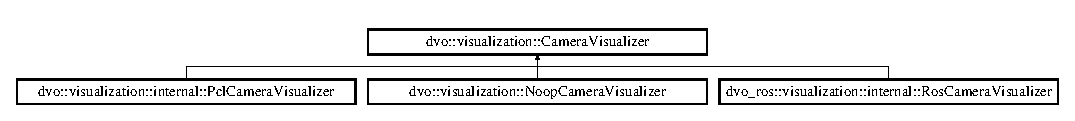
\includegraphics[height=1.181435cm]{classdvo_1_1visualization_1_1_camera_visualizer}
\end{center}
\end{figure}
\subsection*{Public Types}
\begin{DoxyCompactItemize}
\item 
enum \mbox{\hyperlink{classdvo_1_1visualization_1_1_camera_visualizer_a0526f50be9f298c4f7d1f91018d50af7}{Option}} \{ \mbox{\hyperlink{classdvo_1_1visualization_1_1_camera_visualizer_a0526f50be9f298c4f7d1f91018d50af7a0ff8fc7d7283f27066e93ca0d4ef3f19}{Show\+Camera\+And\+Cloud}}, 
\mbox{\hyperlink{classdvo_1_1visualization_1_1_camera_visualizer_a0526f50be9f298c4f7d1f91018d50af7a98873907c6c7542969210d4aedf56e68}{Show\+Camera}}, 
\mbox{\hyperlink{classdvo_1_1visualization_1_1_camera_visualizer_a0526f50be9f298c4f7d1f91018d50af7abb664b1b198725856042bb30de426865}{Show\+Nothing}}
 \}
\item 
typedef boost\+::shared\+\_\+ptr$<$ \mbox{\hyperlink{classdvo_1_1visualization_1_1_camera_visualizer}{Camera\+Visualizer}} $>$ \mbox{\hyperlink{classdvo_1_1visualization_1_1_camera_visualizer_a473ebecc62e1d4edba21027d858789a2}{Ptr}}
\end{DoxyCompactItemize}
\subsection*{Public Member Functions}
\begin{DoxyCompactItemize}
\item 
virtual \mbox{\hyperlink{classdvo_1_1visualization_1_1_camera_visualizer_afa7b81b6dd03ee4f79ce9fc55fce5b91}{$\sim$\+Camera\+Visualizer}} ()
\item 
\mbox{\hyperlink{classdvo_1_1visualization_1_1_camera_visualizer_a4c69b0f2b491852a9a639482e5619fb8}{F\+I\+\_\+\+A\+T\+T\+R\+I\+B\+U\+TE}} (\mbox{\hyperlink{classdvo_1_1visualization_1_1_camera_visualizer}{Camera\+Visualizer}}, std\+::string, name)
\item 
\mbox{\hyperlink{classdvo_1_1visualization_1_1_camera_visualizer_a5f834abd240232041d2c87deedae4d3c}{F\+I\+\_\+\+A\+T\+T\+R\+I\+B\+U\+TE}} (\mbox{\hyperlink{classdvo_1_1visualization_1_1_camera_visualizer}{Camera\+Visualizer}}, \mbox{\hyperlink{structdvo_1_1visualization_1_1_color}{Color}}, color)
\item 
virtual void \mbox{\hyperlink{classdvo_1_1visualization_1_1_camera_visualizer_a646b21ea800d07f6a4174c80daf2bf50}{show}} (\mbox{\hyperlink{classdvo_1_1visualization_1_1_camera_visualizer_a0526f50be9f298c4f7d1f91018d50af7}{Option}} option=\mbox{\hyperlink{classdvo_1_1visualization_1_1_camera_visualizer_a0526f50be9f298c4f7d1f91018d50af7a0ff8fc7d7283f27066e93ca0d4ef3f19}{Show\+Camera\+And\+Cloud}})=0
\item 
virtual void \mbox{\hyperlink{classdvo_1_1visualization_1_1_camera_visualizer_a45dbf0d449a7b7529f7da477c676ca85}{hide}} ()=0
\item 
virtual \mbox{\hyperlink{classdvo_1_1visualization_1_1_camera_visualizer}{Camera\+Visualizer}} \& \mbox{\hyperlink{classdvo_1_1visualization_1_1_camera_visualizer_afd83119e63048b0229820045d54c95ec}{update}} (const \mbox{\hyperlink{structdvo_1_1core_1_1_rgbd_image}{dvo\+::core\+::\+Rgbd\+Image}} \&img, const \mbox{\hyperlink{structdvo_1_1core_1_1_intrinsic_matrix}{dvo\+::core\+::\+Intrinsic\+Matrix}} \&intrinsics, const Eigen\+::\+Affine3d \&pose)=0
\end{DoxyCompactItemize}


\subsection{Member Typedef Documentation}
\mbox{\Hypertarget{classdvo_1_1visualization_1_1_camera_visualizer_a473ebecc62e1d4edba21027d858789a2}\label{classdvo_1_1visualization_1_1_camera_visualizer_a473ebecc62e1d4edba21027d858789a2}} 
\index{dvo\+::visualization\+::\+Camera\+Visualizer@{dvo\+::visualization\+::\+Camera\+Visualizer}!Ptr@{Ptr}}
\index{Ptr@{Ptr}!dvo\+::visualization\+::\+Camera\+Visualizer@{dvo\+::visualization\+::\+Camera\+Visualizer}}
\subsubsection{\texorpdfstring{Ptr}{Ptr}}
{\footnotesize\ttfamily typedef boost\+::shared\+\_\+ptr$<$\mbox{\hyperlink{classdvo_1_1visualization_1_1_camera_visualizer}{Camera\+Visualizer}}$>$ \mbox{\hyperlink{classdvo_1_1visualization_1_1_camera_visualizer_a473ebecc62e1d4edba21027d858789a2}{dvo\+::visualization\+::\+Camera\+Visualizer\+::\+Ptr}}}



\subsection{Member Enumeration Documentation}
\mbox{\Hypertarget{classdvo_1_1visualization_1_1_camera_visualizer_a0526f50be9f298c4f7d1f91018d50af7}\label{classdvo_1_1visualization_1_1_camera_visualizer_a0526f50be9f298c4f7d1f91018d50af7}} 
\index{dvo\+::visualization\+::\+Camera\+Visualizer@{dvo\+::visualization\+::\+Camera\+Visualizer}!Option@{Option}}
\index{Option@{Option}!dvo\+::visualization\+::\+Camera\+Visualizer@{dvo\+::visualization\+::\+Camera\+Visualizer}}
\subsubsection{\texorpdfstring{Option}{Option}}
{\footnotesize\ttfamily enum \mbox{\hyperlink{classdvo_1_1visualization_1_1_camera_visualizer_a0526f50be9f298c4f7d1f91018d50af7}{dvo\+::visualization\+::\+Camera\+Visualizer\+::\+Option}}}

\begin{DoxyEnumFields}{Enumerator}
\raisebox{\heightof{T}}[0pt][0pt]{\index{Show\+Camera\+And\+Cloud@{Show\+Camera\+And\+Cloud}!dvo\+::visualization\+::\+Camera\+Visualizer@{dvo\+::visualization\+::\+Camera\+Visualizer}}\index{dvo\+::visualization\+::\+Camera\+Visualizer@{dvo\+::visualization\+::\+Camera\+Visualizer}!Show\+Camera\+And\+Cloud@{Show\+Camera\+And\+Cloud}}}\mbox{\Hypertarget{classdvo_1_1visualization_1_1_camera_visualizer_a0526f50be9f298c4f7d1f91018d50af7a0ff8fc7d7283f27066e93ca0d4ef3f19}\label{classdvo_1_1visualization_1_1_camera_visualizer_a0526f50be9f298c4f7d1f91018d50af7a0ff8fc7d7283f27066e93ca0d4ef3f19}} 
Show\+Camera\+And\+Cloud&\\
\hline

\raisebox{\heightof{T}}[0pt][0pt]{\index{Show\+Camera@{Show\+Camera}!dvo\+::visualization\+::\+Camera\+Visualizer@{dvo\+::visualization\+::\+Camera\+Visualizer}}\index{dvo\+::visualization\+::\+Camera\+Visualizer@{dvo\+::visualization\+::\+Camera\+Visualizer}!Show\+Camera@{Show\+Camera}}}\mbox{\Hypertarget{classdvo_1_1visualization_1_1_camera_visualizer_a0526f50be9f298c4f7d1f91018d50af7a98873907c6c7542969210d4aedf56e68}\label{classdvo_1_1visualization_1_1_camera_visualizer_a0526f50be9f298c4f7d1f91018d50af7a98873907c6c7542969210d4aedf56e68}} 
Show\+Camera&\\
\hline

\raisebox{\heightof{T}}[0pt][0pt]{\index{Show\+Nothing@{Show\+Nothing}!dvo\+::visualization\+::\+Camera\+Visualizer@{dvo\+::visualization\+::\+Camera\+Visualizer}}\index{dvo\+::visualization\+::\+Camera\+Visualizer@{dvo\+::visualization\+::\+Camera\+Visualizer}!Show\+Nothing@{Show\+Nothing}}}\mbox{\Hypertarget{classdvo_1_1visualization_1_1_camera_visualizer_a0526f50be9f298c4f7d1f91018d50af7abb664b1b198725856042bb30de426865}\label{classdvo_1_1visualization_1_1_camera_visualizer_a0526f50be9f298c4f7d1f91018d50af7abb664b1b198725856042bb30de426865}} 
Show\+Nothing&\\
\hline

\end{DoxyEnumFields}


\subsection{Constructor \& Destructor Documentation}
\mbox{\Hypertarget{classdvo_1_1visualization_1_1_camera_visualizer_afa7b81b6dd03ee4f79ce9fc55fce5b91}\label{classdvo_1_1visualization_1_1_camera_visualizer_afa7b81b6dd03ee4f79ce9fc55fce5b91}} 
\index{dvo\+::visualization\+::\+Camera\+Visualizer@{dvo\+::visualization\+::\+Camera\+Visualizer}!````~Camera\+Visualizer@{$\sim$\+Camera\+Visualizer}}
\index{````~Camera\+Visualizer@{$\sim$\+Camera\+Visualizer}!dvo\+::visualization\+::\+Camera\+Visualizer@{dvo\+::visualization\+::\+Camera\+Visualizer}}
\subsubsection{\texorpdfstring{$\sim$\+Camera\+Visualizer()}{~CameraVisualizer()}}
{\footnotesize\ttfamily virtual dvo\+::visualization\+::\+Camera\+Visualizer\+::$\sim$\+Camera\+Visualizer (\begin{DoxyParamCaption}{ }\end{DoxyParamCaption})\hspace{0.3cm}{\ttfamily [inline]}, {\ttfamily [virtual]}}



\subsection{Member Function Documentation}
\mbox{\Hypertarget{classdvo_1_1visualization_1_1_camera_visualizer_a4c69b0f2b491852a9a639482e5619fb8}\label{classdvo_1_1visualization_1_1_camera_visualizer_a4c69b0f2b491852a9a639482e5619fb8}} 
\index{dvo\+::visualization\+::\+Camera\+Visualizer@{dvo\+::visualization\+::\+Camera\+Visualizer}!F\+I\+\_\+\+A\+T\+T\+R\+I\+B\+U\+TE@{F\+I\+\_\+\+A\+T\+T\+R\+I\+B\+U\+TE}}
\index{F\+I\+\_\+\+A\+T\+T\+R\+I\+B\+U\+TE@{F\+I\+\_\+\+A\+T\+T\+R\+I\+B\+U\+TE}!dvo\+::visualization\+::\+Camera\+Visualizer@{dvo\+::visualization\+::\+Camera\+Visualizer}}
\subsubsection{\texorpdfstring{F\+I\+\_\+\+A\+T\+T\+R\+I\+B\+U\+T\+E()}{FI\_ATTRIBUTE()}\hspace{0.1cm}{\footnotesize\ttfamily [1/2]}}
{\footnotesize\ttfamily dvo\+::visualization\+::\+Camera\+Visualizer\+::\+F\+I\+\_\+\+A\+T\+T\+R\+I\+B\+U\+TE (\begin{DoxyParamCaption}\item[{\mbox{\hyperlink{classdvo_1_1visualization_1_1_camera_visualizer}{Camera\+Visualizer}}}]{,  }\item[{std\+::string}]{,  }\item[{name}]{ }\end{DoxyParamCaption})}

\mbox{\Hypertarget{classdvo_1_1visualization_1_1_camera_visualizer_a5f834abd240232041d2c87deedae4d3c}\label{classdvo_1_1visualization_1_1_camera_visualizer_a5f834abd240232041d2c87deedae4d3c}} 
\index{dvo\+::visualization\+::\+Camera\+Visualizer@{dvo\+::visualization\+::\+Camera\+Visualizer}!F\+I\+\_\+\+A\+T\+T\+R\+I\+B\+U\+TE@{F\+I\+\_\+\+A\+T\+T\+R\+I\+B\+U\+TE}}
\index{F\+I\+\_\+\+A\+T\+T\+R\+I\+B\+U\+TE@{F\+I\+\_\+\+A\+T\+T\+R\+I\+B\+U\+TE}!dvo\+::visualization\+::\+Camera\+Visualizer@{dvo\+::visualization\+::\+Camera\+Visualizer}}
\subsubsection{\texorpdfstring{F\+I\+\_\+\+A\+T\+T\+R\+I\+B\+U\+T\+E()}{FI\_ATTRIBUTE()}\hspace{0.1cm}{\footnotesize\ttfamily [2/2]}}
{\footnotesize\ttfamily dvo\+::visualization\+::\+Camera\+Visualizer\+::\+F\+I\+\_\+\+A\+T\+T\+R\+I\+B\+U\+TE (\begin{DoxyParamCaption}\item[{\mbox{\hyperlink{classdvo_1_1visualization_1_1_camera_visualizer}{Camera\+Visualizer}}}]{,  }\item[{\mbox{\hyperlink{structdvo_1_1visualization_1_1_color}{Color}}}]{,  }\item[{color}]{ }\end{DoxyParamCaption})}

\mbox{\Hypertarget{classdvo_1_1visualization_1_1_camera_visualizer_a45dbf0d449a7b7529f7da477c676ca85}\label{classdvo_1_1visualization_1_1_camera_visualizer_a45dbf0d449a7b7529f7da477c676ca85}} 
\index{dvo\+::visualization\+::\+Camera\+Visualizer@{dvo\+::visualization\+::\+Camera\+Visualizer}!hide@{hide}}
\index{hide@{hide}!dvo\+::visualization\+::\+Camera\+Visualizer@{dvo\+::visualization\+::\+Camera\+Visualizer}}
\subsubsection{\texorpdfstring{hide()}{hide()}}
{\footnotesize\ttfamily virtual void dvo\+::visualization\+::\+Camera\+Visualizer\+::hide (\begin{DoxyParamCaption}{ }\end{DoxyParamCaption})\hspace{0.3cm}{\ttfamily [pure virtual]}}



Implemented in \mbox{\hyperlink{classdvo_1_1visualization_1_1internal_1_1_pcl_camera_visualizer_ad261307239a87bc10ba4d0662960cc72}{dvo\+::visualization\+::internal\+::\+Pcl\+Camera\+Visualizer}}, \mbox{\hyperlink{classdvo__ros_1_1visualization_1_1internal_1_1_ros_camera_visualizer_a4812a8e3c5573a68fb74cabbf2f70422}{dvo\+\_\+ros\+::visualization\+::internal\+::\+Ros\+Camera\+Visualizer}}, and \mbox{\hyperlink{classdvo_1_1visualization_1_1_noop_camera_visualizer_a875ff591e3db513ddbec48478989639e}{dvo\+::visualization\+::\+Noop\+Camera\+Visualizer}}.

\mbox{\Hypertarget{classdvo_1_1visualization_1_1_camera_visualizer_a646b21ea800d07f6a4174c80daf2bf50}\label{classdvo_1_1visualization_1_1_camera_visualizer_a646b21ea800d07f6a4174c80daf2bf50}} 
\index{dvo\+::visualization\+::\+Camera\+Visualizer@{dvo\+::visualization\+::\+Camera\+Visualizer}!show@{show}}
\index{show@{show}!dvo\+::visualization\+::\+Camera\+Visualizer@{dvo\+::visualization\+::\+Camera\+Visualizer}}
\subsubsection{\texorpdfstring{show()}{show()}}
{\footnotesize\ttfamily virtual void dvo\+::visualization\+::\+Camera\+Visualizer\+::show (\begin{DoxyParamCaption}\item[{\mbox{\hyperlink{classdvo_1_1visualization_1_1_camera_visualizer_a0526f50be9f298c4f7d1f91018d50af7}{Option}}}]{option = {\ttfamily \mbox{\hyperlink{classdvo_1_1visualization_1_1_camera_visualizer_a0526f50be9f298c4f7d1f91018d50af7a0ff8fc7d7283f27066e93ca0d4ef3f19}{Show\+Camera\+And\+Cloud}}} }\end{DoxyParamCaption})\hspace{0.3cm}{\ttfamily [pure virtual]}}



Implemented in \mbox{\hyperlink{classdvo_1_1visualization_1_1internal_1_1_pcl_camera_visualizer_a09b5d8117f8ca15489ac42f6b6019030}{dvo\+::visualization\+::internal\+::\+Pcl\+Camera\+Visualizer}}, and \mbox{\hyperlink{classdvo_1_1visualization_1_1_noop_camera_visualizer_acfb97efacfcb9e3dd30444e34c7bfd9c}{dvo\+::visualization\+::\+Noop\+Camera\+Visualizer}}.

\mbox{\Hypertarget{classdvo_1_1visualization_1_1_camera_visualizer_afd83119e63048b0229820045d54c95ec}\label{classdvo_1_1visualization_1_1_camera_visualizer_afd83119e63048b0229820045d54c95ec}} 
\index{dvo\+::visualization\+::\+Camera\+Visualizer@{dvo\+::visualization\+::\+Camera\+Visualizer}!update@{update}}
\index{update@{update}!dvo\+::visualization\+::\+Camera\+Visualizer@{dvo\+::visualization\+::\+Camera\+Visualizer}}
\subsubsection{\texorpdfstring{update()}{update()}}
{\footnotesize\ttfamily virtual \mbox{\hyperlink{classdvo_1_1visualization_1_1_camera_visualizer}{Camera\+Visualizer}}\& dvo\+::visualization\+::\+Camera\+Visualizer\+::update (\begin{DoxyParamCaption}\item[{const \mbox{\hyperlink{structdvo_1_1core_1_1_rgbd_image}{dvo\+::core\+::\+Rgbd\+Image}} \&}]{img,  }\item[{const \mbox{\hyperlink{structdvo_1_1core_1_1_intrinsic_matrix}{dvo\+::core\+::\+Intrinsic\+Matrix}} \&}]{intrinsics,  }\item[{const Eigen\+::\+Affine3d \&}]{pose }\end{DoxyParamCaption})\hspace{0.3cm}{\ttfamily [pure virtual]}}



Implemented in \mbox{\hyperlink{classdvo_1_1visualization_1_1internal_1_1_pcl_camera_visualizer_adfe2b8752f78ee0fa6ee193be70941eb}{dvo\+::visualization\+::internal\+::\+Pcl\+Camera\+Visualizer}}, \mbox{\hyperlink{classdvo__ros_1_1visualization_1_1internal_1_1_ros_camera_visualizer_aa347218752bde73e09874771fe3b4410}{dvo\+\_\+ros\+::visualization\+::internal\+::\+Ros\+Camera\+Visualizer}}, and \mbox{\hyperlink{classdvo_1_1visualization_1_1_noop_camera_visualizer_a7983d8de9de45c5617c3e877d36d6ff3}{dvo\+::visualization\+::\+Noop\+Camera\+Visualizer}}.



The documentation for this class was generated from the following file\+:\begin{DoxyCompactItemize}
\item 
dvo\+\_\+core/include/dvo/visualization/\mbox{\hyperlink{camera__trajectory__visualizer_8h}{camera\+\_\+trajectory\+\_\+visualizer.\+h}}\end{DoxyCompactItemize}

\hypertarget{structdvo_1_1visualization_1_1_color}{}\section{dvo\+:\+:visualization\+:\+:Color Struct Reference}
\label{structdvo_1_1visualization_1_1_color}\index{dvo\+::visualization\+::\+Color@{dvo\+::visualization\+::\+Color}}


{\ttfamily \#include $<$camera\+\_\+trajectory\+\_\+visualizer.\+h$>$}

\subsection*{Public Member Functions}
\begin{DoxyCompactItemize}
\item 
\mbox{\hyperlink{structdvo_1_1visualization_1_1_color_a512f756a2cca890e6157d655691b7282}{Color}} ()
\item 
\mbox{\hyperlink{structdvo_1_1visualization_1_1_color_ae045be10ad75fe12f0962ed5f36f458e}{Color}} (double \mbox{\hyperlink{structdvo_1_1visualization_1_1_color_a6941dd0d782ff4ecb73e0b4b0ac90f34}{r}}, double \mbox{\hyperlink{structdvo_1_1visualization_1_1_color_a683bddf0b9bd3d6d8a229a25a68d20b0}{g}}, double \mbox{\hyperlink{structdvo_1_1visualization_1_1_color_af48f0b94f4bd5e44fba8f039e8b9147d}{b}})
\end{DoxyCompactItemize}
\subsection*{Static Public Member Functions}
\begin{DoxyCompactItemize}
\item 
static const \mbox{\hyperlink{structdvo_1_1visualization_1_1_color}{Color}} \& \mbox{\hyperlink{structdvo_1_1visualization_1_1_color_afe1b33e3675419d460c9826073e45b23}{red}} ()
\item 
static const \mbox{\hyperlink{structdvo_1_1visualization_1_1_color}{Color}} \& \mbox{\hyperlink{structdvo_1_1visualization_1_1_color_a9a4cea43a6ad4ac6aef4dfe17ef6acd5}{green}} ()
\item 
static const \mbox{\hyperlink{structdvo_1_1visualization_1_1_color}{Color}} \& \mbox{\hyperlink{structdvo_1_1visualization_1_1_color_a82e356c5191e2f73ca16f1ae96abca30}{blue}} ()
\end{DoxyCompactItemize}
\subsection*{Public Attributes}
\begin{DoxyCompactItemize}
\item 
double \mbox{\hyperlink{structdvo_1_1visualization_1_1_color_a6941dd0d782ff4ecb73e0b4b0ac90f34}{r}}
\item 
double \mbox{\hyperlink{structdvo_1_1visualization_1_1_color_a683bddf0b9bd3d6d8a229a25a68d20b0}{g}}
\item 
double \mbox{\hyperlink{structdvo_1_1visualization_1_1_color_af48f0b94f4bd5e44fba8f039e8b9147d}{b}}
\end{DoxyCompactItemize}


\subsection{Constructor \& Destructor Documentation}
\mbox{\Hypertarget{structdvo_1_1visualization_1_1_color_a512f756a2cca890e6157d655691b7282}\label{structdvo_1_1visualization_1_1_color_a512f756a2cca890e6157d655691b7282}} 
\index{dvo\+::visualization\+::\+Color@{dvo\+::visualization\+::\+Color}!Color@{Color}}
\index{Color@{Color}!dvo\+::visualization\+::\+Color@{dvo\+::visualization\+::\+Color}}
\subsubsection{\texorpdfstring{Color()}{Color()}\hspace{0.1cm}{\footnotesize\ttfamily [1/2]}}
{\footnotesize\ttfamily dvo\+::visualization\+::\+Color\+::\+Color (\begin{DoxyParamCaption}{ }\end{DoxyParamCaption})\hspace{0.3cm}{\ttfamily [inline]}}

\mbox{\Hypertarget{structdvo_1_1visualization_1_1_color_ae045be10ad75fe12f0962ed5f36f458e}\label{structdvo_1_1visualization_1_1_color_ae045be10ad75fe12f0962ed5f36f458e}} 
\index{dvo\+::visualization\+::\+Color@{dvo\+::visualization\+::\+Color}!Color@{Color}}
\index{Color@{Color}!dvo\+::visualization\+::\+Color@{dvo\+::visualization\+::\+Color}}
\subsubsection{\texorpdfstring{Color()}{Color()}\hspace{0.1cm}{\footnotesize\ttfamily [2/2]}}
{\footnotesize\ttfamily dvo\+::visualization\+::\+Color\+::\+Color (\begin{DoxyParamCaption}\item[{double}]{r,  }\item[{double}]{g,  }\item[{double}]{b }\end{DoxyParamCaption})\hspace{0.3cm}{\ttfamily [inline]}}



\subsection{Member Function Documentation}
\mbox{\Hypertarget{structdvo_1_1visualization_1_1_color_a82e356c5191e2f73ca16f1ae96abca30}\label{structdvo_1_1visualization_1_1_color_a82e356c5191e2f73ca16f1ae96abca30}} 
\index{dvo\+::visualization\+::\+Color@{dvo\+::visualization\+::\+Color}!blue@{blue}}
\index{blue@{blue}!dvo\+::visualization\+::\+Color@{dvo\+::visualization\+::\+Color}}
\subsubsection{\texorpdfstring{blue()}{blue()}}
{\footnotesize\ttfamily static const \mbox{\hyperlink{structdvo_1_1visualization_1_1_color}{Color}}\& dvo\+::visualization\+::\+Color\+::blue (\begin{DoxyParamCaption}{ }\end{DoxyParamCaption})\hspace{0.3cm}{\ttfamily [inline]}, {\ttfamily [static]}}

\mbox{\Hypertarget{structdvo_1_1visualization_1_1_color_a9a4cea43a6ad4ac6aef4dfe17ef6acd5}\label{structdvo_1_1visualization_1_1_color_a9a4cea43a6ad4ac6aef4dfe17ef6acd5}} 
\index{dvo\+::visualization\+::\+Color@{dvo\+::visualization\+::\+Color}!green@{green}}
\index{green@{green}!dvo\+::visualization\+::\+Color@{dvo\+::visualization\+::\+Color}}
\subsubsection{\texorpdfstring{green()}{green()}}
{\footnotesize\ttfamily static const \mbox{\hyperlink{structdvo_1_1visualization_1_1_color}{Color}}\& dvo\+::visualization\+::\+Color\+::green (\begin{DoxyParamCaption}{ }\end{DoxyParamCaption})\hspace{0.3cm}{\ttfamily [inline]}, {\ttfamily [static]}}

\mbox{\Hypertarget{structdvo_1_1visualization_1_1_color_afe1b33e3675419d460c9826073e45b23}\label{structdvo_1_1visualization_1_1_color_afe1b33e3675419d460c9826073e45b23}} 
\index{dvo\+::visualization\+::\+Color@{dvo\+::visualization\+::\+Color}!red@{red}}
\index{red@{red}!dvo\+::visualization\+::\+Color@{dvo\+::visualization\+::\+Color}}
\subsubsection{\texorpdfstring{red()}{red()}}
{\footnotesize\ttfamily static const \mbox{\hyperlink{structdvo_1_1visualization_1_1_color}{Color}}\& dvo\+::visualization\+::\+Color\+::red (\begin{DoxyParamCaption}{ }\end{DoxyParamCaption})\hspace{0.3cm}{\ttfamily [inline]}, {\ttfamily [static]}}



\subsection{Member Data Documentation}
\mbox{\Hypertarget{structdvo_1_1visualization_1_1_color_af48f0b94f4bd5e44fba8f039e8b9147d}\label{structdvo_1_1visualization_1_1_color_af48f0b94f4bd5e44fba8f039e8b9147d}} 
\index{dvo\+::visualization\+::\+Color@{dvo\+::visualization\+::\+Color}!b@{b}}
\index{b@{b}!dvo\+::visualization\+::\+Color@{dvo\+::visualization\+::\+Color}}
\subsubsection{\texorpdfstring{b}{b}}
{\footnotesize\ttfamily double dvo\+::visualization\+::\+Color\+::b}

\mbox{\Hypertarget{structdvo_1_1visualization_1_1_color_a683bddf0b9bd3d6d8a229a25a68d20b0}\label{structdvo_1_1visualization_1_1_color_a683bddf0b9bd3d6d8a229a25a68d20b0}} 
\index{dvo\+::visualization\+::\+Color@{dvo\+::visualization\+::\+Color}!g@{g}}
\index{g@{g}!dvo\+::visualization\+::\+Color@{dvo\+::visualization\+::\+Color}}
\subsubsection{\texorpdfstring{g}{g}}
{\footnotesize\ttfamily double dvo\+::visualization\+::\+Color\+::g}

\mbox{\Hypertarget{structdvo_1_1visualization_1_1_color_a6941dd0d782ff4ecb73e0b4b0ac90f34}\label{structdvo_1_1visualization_1_1_color_a6941dd0d782ff4ecb73e0b4b0ac90f34}} 
\index{dvo\+::visualization\+::\+Color@{dvo\+::visualization\+::\+Color}!r@{r}}
\index{r@{r}!dvo\+::visualization\+::\+Color@{dvo\+::visualization\+::\+Color}}
\subsubsection{\texorpdfstring{r}{r}}
{\footnotesize\ttfamily double dvo\+::visualization\+::\+Color\+::r}



The documentation for this struct was generated from the following file\+:\begin{DoxyCompactItemize}
\item 
dvo\+\_\+core/include/dvo/visualization/\mbox{\hyperlink{camera__trajectory__visualizer_8h}{camera\+\_\+trajectory\+\_\+visualizer.\+h}}\end{DoxyCompactItemize}

\hypertarget{structdvo_1_1_dense_tracker_1_1_config}{}\section{dvo\+:\+:Dense\+Tracker\+:\+:Config Struct Reference}
\label{structdvo_1_1_dense_tracker_1_1_config}\index{dvo\+::\+Dense\+Tracker\+::\+Config@{dvo\+::\+Dense\+Tracker\+::\+Config}}


{\ttfamily \#include $<$dense\+\_\+tracking.\+h$>$}

\subsection*{Public Member Functions}
\begin{DoxyCompactItemize}
\item 
\mbox{\hyperlink{structdvo_1_1_dense_tracker_1_1_config_af31c5a1d23a1516b2dd2a144f9593dc3}{Config}} ()
\item 
size\+\_\+t \mbox{\hyperlink{structdvo_1_1_dense_tracker_1_1_config_a45695687943199e6a16004986f96b479}{get\+Num\+Levels}} () const
\item 
bool \mbox{\hyperlink{structdvo_1_1_dense_tracker_1_1_config_a4530028334aa41483d8c3df3a92e7890}{Use\+Temporal\+Smoothing}} () const
\item 
bool \mbox{\hyperlink{structdvo_1_1_dense_tracker_1_1_config_a5aaf59dfe2495c19cbe6e759cc35f1b5}{Use\+Estimate\+Smoothing}} () const
\item 
bool \mbox{\hyperlink{structdvo_1_1_dense_tracker_1_1_config_a7a4028e633393e3bc45c3637aba924d4}{Is\+Sane}} () const
\end{DoxyCompactItemize}
\subsection*{Public Attributes}
\begin{DoxyCompactItemize}
\item 
int \mbox{\hyperlink{structdvo_1_1_dense_tracker_1_1_config_af07fb088139f396d4bb19098ef263131}{First\+Level}}
\item 
int \mbox{\hyperlink{structdvo_1_1_dense_tracker_1_1_config_ae96df17e33f1193c3ab6fbf5efc930dd}{Last\+Level}}
\item 
int \mbox{\hyperlink{structdvo_1_1_dense_tracker_1_1_config_a80800ec37764ee5104923d43aad84ce4}{Max\+Iterations\+Per\+Level}}
\item 
double \mbox{\hyperlink{structdvo_1_1_dense_tracker_1_1_config_abc739e291273bf79606cfe4963ee5ab4}{Precision}}
\item 
double \mbox{\hyperlink{structdvo_1_1_dense_tracker_1_1_config_ae54b4a38091ee23d984afa4394131082}{Lambda}}
\item 
double \mbox{\hyperlink{structdvo_1_1_dense_tracker_1_1_config_ad730897eef6700450f9a96f1712fde41}{Mu}}
\item 
bool \mbox{\hyperlink{structdvo_1_1_dense_tracker_1_1_config_a2fa85ee168aa0bbd24aee72f97943a85}{Use\+Initial\+Estimate}}
\item 
bool \mbox{\hyperlink{structdvo_1_1_dense_tracker_1_1_config_a42ef85cd4907ab5c65b37a17ad1315d4}{Use\+Weighting}}
\item 
\mbox{\hyperlink{structdvo_1_1core_1_1_influence_functions_a3fcb0831eb60e196888641a64fff665f}{dvo\+::core\+::\+Influence\+Functions\+::enum\+\_\+t}} \mbox{\hyperlink{structdvo_1_1_dense_tracker_1_1_config_a464bdce67b2fb96a49808bae1c9c775a}{Influence\+Funtion\+Type}}
\item 
float \mbox{\hyperlink{structdvo_1_1_dense_tracker_1_1_config_a87ea8193f2e731a76cba63e56a853009}{Influence\+Function\+Param}}
\item 
\mbox{\hyperlink{structdvo_1_1core_1_1_scale_estimators_a5bd47dbbdca475d830703b07b0864f5e}{dvo\+::core\+::\+Scale\+Estimators\+::enum\+\_\+t}} \mbox{\hyperlink{structdvo_1_1_dense_tracker_1_1_config_a9b902aa9f9ffbca70b38edb9416ddbf8}{Scale\+Estimator\+Type}}
\item 
float \mbox{\hyperlink{structdvo_1_1_dense_tracker_1_1_config_a5477e9a5a7e8da5e066db1446211bf51}{Scale\+Estimator\+Param}}
\end{DoxyCompactItemize}


\subsection{Constructor \& Destructor Documentation}
\mbox{\Hypertarget{structdvo_1_1_dense_tracker_1_1_config_af31c5a1d23a1516b2dd2a144f9593dc3}\label{structdvo_1_1_dense_tracker_1_1_config_af31c5a1d23a1516b2dd2a144f9593dc3}} 
\index{dvo\+::\+Dense\+Tracker\+::\+Config@{dvo\+::\+Dense\+Tracker\+::\+Config}!Config@{Config}}
\index{Config@{Config}!dvo\+::\+Dense\+Tracker\+::\+Config@{dvo\+::\+Dense\+Tracker\+::\+Config}}
\subsubsection{\texorpdfstring{Config()}{Config()}}
{\footnotesize\ttfamily dvo\+::\+Dense\+Tracker\+::\+Config\+::\+Config (\begin{DoxyParamCaption}{ }\end{DoxyParamCaption})}



\subsection{Member Function Documentation}
\mbox{\Hypertarget{structdvo_1_1_dense_tracker_1_1_config_a45695687943199e6a16004986f96b479}\label{structdvo_1_1_dense_tracker_1_1_config_a45695687943199e6a16004986f96b479}} 
\index{dvo\+::\+Dense\+Tracker\+::\+Config@{dvo\+::\+Dense\+Tracker\+::\+Config}!get\+Num\+Levels@{get\+Num\+Levels}}
\index{get\+Num\+Levels@{get\+Num\+Levels}!dvo\+::\+Dense\+Tracker\+::\+Config@{dvo\+::\+Dense\+Tracker\+::\+Config}}
\subsubsection{\texorpdfstring{get\+Num\+Levels()}{getNumLevels()}}
{\footnotesize\ttfamily size\+\_\+t dvo\+::\+Dense\+Tracker\+::\+Config\+::get\+Num\+Levels (\begin{DoxyParamCaption}{ }\end{DoxyParamCaption}) const}

\mbox{\Hypertarget{structdvo_1_1_dense_tracker_1_1_config_a7a4028e633393e3bc45c3637aba924d4}\label{structdvo_1_1_dense_tracker_1_1_config_a7a4028e633393e3bc45c3637aba924d4}} 
\index{dvo\+::\+Dense\+Tracker\+::\+Config@{dvo\+::\+Dense\+Tracker\+::\+Config}!Is\+Sane@{Is\+Sane}}
\index{Is\+Sane@{Is\+Sane}!dvo\+::\+Dense\+Tracker\+::\+Config@{dvo\+::\+Dense\+Tracker\+::\+Config}}
\subsubsection{\texorpdfstring{Is\+Sane()}{IsSane()}}
{\footnotesize\ttfamily bool dvo\+::\+Dense\+Tracker\+::\+Config\+::\+Is\+Sane (\begin{DoxyParamCaption}{ }\end{DoxyParamCaption}) const}

\mbox{\Hypertarget{structdvo_1_1_dense_tracker_1_1_config_a5aaf59dfe2495c19cbe6e759cc35f1b5}\label{structdvo_1_1_dense_tracker_1_1_config_a5aaf59dfe2495c19cbe6e759cc35f1b5}} 
\index{dvo\+::\+Dense\+Tracker\+::\+Config@{dvo\+::\+Dense\+Tracker\+::\+Config}!Use\+Estimate\+Smoothing@{Use\+Estimate\+Smoothing}}
\index{Use\+Estimate\+Smoothing@{Use\+Estimate\+Smoothing}!dvo\+::\+Dense\+Tracker\+::\+Config@{dvo\+::\+Dense\+Tracker\+::\+Config}}
\subsubsection{\texorpdfstring{Use\+Estimate\+Smoothing()}{UseEstimateSmoothing()}}
{\footnotesize\ttfamily bool dvo\+::\+Dense\+Tracker\+::\+Config\+::\+Use\+Estimate\+Smoothing (\begin{DoxyParamCaption}{ }\end{DoxyParamCaption}) const}

\mbox{\Hypertarget{structdvo_1_1_dense_tracker_1_1_config_a4530028334aa41483d8c3df3a92e7890}\label{structdvo_1_1_dense_tracker_1_1_config_a4530028334aa41483d8c3df3a92e7890}} 
\index{dvo\+::\+Dense\+Tracker\+::\+Config@{dvo\+::\+Dense\+Tracker\+::\+Config}!Use\+Temporal\+Smoothing@{Use\+Temporal\+Smoothing}}
\index{Use\+Temporal\+Smoothing@{Use\+Temporal\+Smoothing}!dvo\+::\+Dense\+Tracker\+::\+Config@{dvo\+::\+Dense\+Tracker\+::\+Config}}
\subsubsection{\texorpdfstring{Use\+Temporal\+Smoothing()}{UseTemporalSmoothing()}}
{\footnotesize\ttfamily bool dvo\+::\+Dense\+Tracker\+::\+Config\+::\+Use\+Temporal\+Smoothing (\begin{DoxyParamCaption}{ }\end{DoxyParamCaption}) const}



\subsection{Member Data Documentation}
\mbox{\Hypertarget{structdvo_1_1_dense_tracker_1_1_config_af07fb088139f396d4bb19098ef263131}\label{structdvo_1_1_dense_tracker_1_1_config_af07fb088139f396d4bb19098ef263131}} 
\index{dvo\+::\+Dense\+Tracker\+::\+Config@{dvo\+::\+Dense\+Tracker\+::\+Config}!First\+Level@{First\+Level}}
\index{First\+Level@{First\+Level}!dvo\+::\+Dense\+Tracker\+::\+Config@{dvo\+::\+Dense\+Tracker\+::\+Config}}
\subsubsection{\texorpdfstring{First\+Level}{FirstLevel}}
{\footnotesize\ttfamily int dvo\+::\+Dense\+Tracker\+::\+Config\+::\+First\+Level}

\mbox{\Hypertarget{structdvo_1_1_dense_tracker_1_1_config_a87ea8193f2e731a76cba63e56a853009}\label{structdvo_1_1_dense_tracker_1_1_config_a87ea8193f2e731a76cba63e56a853009}} 
\index{dvo\+::\+Dense\+Tracker\+::\+Config@{dvo\+::\+Dense\+Tracker\+::\+Config}!Influence\+Function\+Param@{Influence\+Function\+Param}}
\index{Influence\+Function\+Param@{Influence\+Function\+Param}!dvo\+::\+Dense\+Tracker\+::\+Config@{dvo\+::\+Dense\+Tracker\+::\+Config}}
\subsubsection{\texorpdfstring{Influence\+Function\+Param}{InfluenceFunctionParam}}
{\footnotesize\ttfamily float dvo\+::\+Dense\+Tracker\+::\+Config\+::\+Influence\+Function\+Param}

\mbox{\Hypertarget{structdvo_1_1_dense_tracker_1_1_config_a464bdce67b2fb96a49808bae1c9c775a}\label{structdvo_1_1_dense_tracker_1_1_config_a464bdce67b2fb96a49808bae1c9c775a}} 
\index{dvo\+::\+Dense\+Tracker\+::\+Config@{dvo\+::\+Dense\+Tracker\+::\+Config}!Influence\+Funtion\+Type@{Influence\+Funtion\+Type}}
\index{Influence\+Funtion\+Type@{Influence\+Funtion\+Type}!dvo\+::\+Dense\+Tracker\+::\+Config@{dvo\+::\+Dense\+Tracker\+::\+Config}}
\subsubsection{\texorpdfstring{Influence\+Funtion\+Type}{InfluenceFuntionType}}
{\footnotesize\ttfamily \mbox{\hyperlink{structdvo_1_1core_1_1_influence_functions_a3fcb0831eb60e196888641a64fff665f}{dvo\+::core\+::\+Influence\+Functions\+::enum\+\_\+t}} dvo\+::\+Dense\+Tracker\+::\+Config\+::\+Influence\+Funtion\+Type}

\mbox{\Hypertarget{structdvo_1_1_dense_tracker_1_1_config_ae54b4a38091ee23d984afa4394131082}\label{structdvo_1_1_dense_tracker_1_1_config_ae54b4a38091ee23d984afa4394131082}} 
\index{dvo\+::\+Dense\+Tracker\+::\+Config@{dvo\+::\+Dense\+Tracker\+::\+Config}!Lambda@{Lambda}}
\index{Lambda@{Lambda}!dvo\+::\+Dense\+Tracker\+::\+Config@{dvo\+::\+Dense\+Tracker\+::\+Config}}
\subsubsection{\texorpdfstring{Lambda}{Lambda}}
{\footnotesize\ttfamily double dvo\+::\+Dense\+Tracker\+::\+Config\+::\+Lambda}

\mbox{\Hypertarget{structdvo_1_1_dense_tracker_1_1_config_ae96df17e33f1193c3ab6fbf5efc930dd}\label{structdvo_1_1_dense_tracker_1_1_config_ae96df17e33f1193c3ab6fbf5efc930dd}} 
\index{dvo\+::\+Dense\+Tracker\+::\+Config@{dvo\+::\+Dense\+Tracker\+::\+Config}!Last\+Level@{Last\+Level}}
\index{Last\+Level@{Last\+Level}!dvo\+::\+Dense\+Tracker\+::\+Config@{dvo\+::\+Dense\+Tracker\+::\+Config}}
\subsubsection{\texorpdfstring{Last\+Level}{LastLevel}}
{\footnotesize\ttfamily int dvo\+::\+Dense\+Tracker\+::\+Config\+::\+Last\+Level}

\mbox{\Hypertarget{structdvo_1_1_dense_tracker_1_1_config_a80800ec37764ee5104923d43aad84ce4}\label{structdvo_1_1_dense_tracker_1_1_config_a80800ec37764ee5104923d43aad84ce4}} 
\index{dvo\+::\+Dense\+Tracker\+::\+Config@{dvo\+::\+Dense\+Tracker\+::\+Config}!Max\+Iterations\+Per\+Level@{Max\+Iterations\+Per\+Level}}
\index{Max\+Iterations\+Per\+Level@{Max\+Iterations\+Per\+Level}!dvo\+::\+Dense\+Tracker\+::\+Config@{dvo\+::\+Dense\+Tracker\+::\+Config}}
\subsubsection{\texorpdfstring{Max\+Iterations\+Per\+Level}{MaxIterationsPerLevel}}
{\footnotesize\ttfamily int dvo\+::\+Dense\+Tracker\+::\+Config\+::\+Max\+Iterations\+Per\+Level}

\mbox{\Hypertarget{structdvo_1_1_dense_tracker_1_1_config_ad730897eef6700450f9a96f1712fde41}\label{structdvo_1_1_dense_tracker_1_1_config_ad730897eef6700450f9a96f1712fde41}} 
\index{dvo\+::\+Dense\+Tracker\+::\+Config@{dvo\+::\+Dense\+Tracker\+::\+Config}!Mu@{Mu}}
\index{Mu@{Mu}!dvo\+::\+Dense\+Tracker\+::\+Config@{dvo\+::\+Dense\+Tracker\+::\+Config}}
\subsubsection{\texorpdfstring{Mu}{Mu}}
{\footnotesize\ttfamily double dvo\+::\+Dense\+Tracker\+::\+Config\+::\+Mu}

\mbox{\Hypertarget{structdvo_1_1_dense_tracker_1_1_config_abc739e291273bf79606cfe4963ee5ab4}\label{structdvo_1_1_dense_tracker_1_1_config_abc739e291273bf79606cfe4963ee5ab4}} 
\index{dvo\+::\+Dense\+Tracker\+::\+Config@{dvo\+::\+Dense\+Tracker\+::\+Config}!Precision@{Precision}}
\index{Precision@{Precision}!dvo\+::\+Dense\+Tracker\+::\+Config@{dvo\+::\+Dense\+Tracker\+::\+Config}}
\subsubsection{\texorpdfstring{Precision}{Precision}}
{\footnotesize\ttfamily double dvo\+::\+Dense\+Tracker\+::\+Config\+::\+Precision}

\mbox{\Hypertarget{structdvo_1_1_dense_tracker_1_1_config_a5477e9a5a7e8da5e066db1446211bf51}\label{structdvo_1_1_dense_tracker_1_1_config_a5477e9a5a7e8da5e066db1446211bf51}} 
\index{dvo\+::\+Dense\+Tracker\+::\+Config@{dvo\+::\+Dense\+Tracker\+::\+Config}!Scale\+Estimator\+Param@{Scale\+Estimator\+Param}}
\index{Scale\+Estimator\+Param@{Scale\+Estimator\+Param}!dvo\+::\+Dense\+Tracker\+::\+Config@{dvo\+::\+Dense\+Tracker\+::\+Config}}
\subsubsection{\texorpdfstring{Scale\+Estimator\+Param}{ScaleEstimatorParam}}
{\footnotesize\ttfamily float dvo\+::\+Dense\+Tracker\+::\+Config\+::\+Scale\+Estimator\+Param}

\mbox{\Hypertarget{structdvo_1_1_dense_tracker_1_1_config_a9b902aa9f9ffbca70b38edb9416ddbf8}\label{structdvo_1_1_dense_tracker_1_1_config_a9b902aa9f9ffbca70b38edb9416ddbf8}} 
\index{dvo\+::\+Dense\+Tracker\+::\+Config@{dvo\+::\+Dense\+Tracker\+::\+Config}!Scale\+Estimator\+Type@{Scale\+Estimator\+Type}}
\index{Scale\+Estimator\+Type@{Scale\+Estimator\+Type}!dvo\+::\+Dense\+Tracker\+::\+Config@{dvo\+::\+Dense\+Tracker\+::\+Config}}
\subsubsection{\texorpdfstring{Scale\+Estimator\+Type}{ScaleEstimatorType}}
{\footnotesize\ttfamily \mbox{\hyperlink{structdvo_1_1core_1_1_scale_estimators_a5bd47dbbdca475d830703b07b0864f5e}{dvo\+::core\+::\+Scale\+Estimators\+::enum\+\_\+t}} dvo\+::\+Dense\+Tracker\+::\+Config\+::\+Scale\+Estimator\+Type}

\mbox{\Hypertarget{structdvo_1_1_dense_tracker_1_1_config_a2fa85ee168aa0bbd24aee72f97943a85}\label{structdvo_1_1_dense_tracker_1_1_config_a2fa85ee168aa0bbd24aee72f97943a85}} 
\index{dvo\+::\+Dense\+Tracker\+::\+Config@{dvo\+::\+Dense\+Tracker\+::\+Config}!Use\+Initial\+Estimate@{Use\+Initial\+Estimate}}
\index{Use\+Initial\+Estimate@{Use\+Initial\+Estimate}!dvo\+::\+Dense\+Tracker\+::\+Config@{dvo\+::\+Dense\+Tracker\+::\+Config}}
\subsubsection{\texorpdfstring{Use\+Initial\+Estimate}{UseInitialEstimate}}
{\footnotesize\ttfamily bool dvo\+::\+Dense\+Tracker\+::\+Config\+::\+Use\+Initial\+Estimate}

\mbox{\Hypertarget{structdvo_1_1_dense_tracker_1_1_config_a42ef85cd4907ab5c65b37a17ad1315d4}\label{structdvo_1_1_dense_tracker_1_1_config_a42ef85cd4907ab5c65b37a17ad1315d4}} 
\index{dvo\+::\+Dense\+Tracker\+::\+Config@{dvo\+::\+Dense\+Tracker\+::\+Config}!Use\+Weighting@{Use\+Weighting}}
\index{Use\+Weighting@{Use\+Weighting}!dvo\+::\+Dense\+Tracker\+::\+Config@{dvo\+::\+Dense\+Tracker\+::\+Config}}
\subsubsection{\texorpdfstring{Use\+Weighting}{UseWeighting}}
{\footnotesize\ttfamily bool dvo\+::\+Dense\+Tracker\+::\+Config\+::\+Use\+Weighting}



The documentation for this struct was generated from the following files\+:\begin{DoxyCompactItemize}
\item 
dvo\+\_\+core/include/dvo/\mbox{\hyperlink{dense__tracking_8h}{dense\+\_\+tracking.\+h}}\item 
dvo\+\_\+core/src/\mbox{\hyperlink{dense__tracking__config_8cpp}{dense\+\_\+tracking\+\_\+config.\+cpp}}\end{DoxyCompactItemize}

\hypertarget{struct_benchmark_node_1_1_config}{}\section{Benchmark\+Node\+:\+:Config Struct Reference}
\label{struct_benchmark_node_1_1_config}\index{Benchmark\+Node\+::\+Config@{Benchmark\+Node\+::\+Config}}
\subsection*{Public Member Functions}
\begin{DoxyCompactItemize}
\item 
bool \mbox{\hyperlink{struct_benchmark_node_1_1_config_ab4f05c5481c41507101a0ab04ce5587f}{Estimate\+Required}} ()
\item 
bool \mbox{\hyperlink{struct_benchmark_node_1_1_config_a44784806c6a028e9da922ae980cd94bb}{Visualization\+Required}} ()
\end{DoxyCompactItemize}
\subsection*{Public Attributes}
\begin{DoxyCompactItemize}
\item 
bool \mbox{\hyperlink{struct_benchmark_node_1_1_config_a824720538ff9542fe44934dd60a0f271}{Estimate\+Trajectory}}
\item 
std\+::string \mbox{\hyperlink{struct_benchmark_node_1_1_config_aba679b0c17d5f218d4fd20793621cb0b}{Trajectory\+File}}
\item 
bool \mbox{\hyperlink{struct_benchmark_node_1_1_config_a72d3251a5b7caaab8e57a8af80a730b6}{Render\+Video}}
\item 
std\+::string \mbox{\hyperlink{struct_benchmark_node_1_1_config_a48d6c0a184764fa7fc9fede1dc2616fa}{Video\+Folder}}
\item 
std\+::string \mbox{\hyperlink{struct_benchmark_node_1_1_config_a042bfe6e38d694ad33ad8df4b60212a6}{Camera\+File}}
\item 
std\+::string \mbox{\hyperlink{struct_benchmark_node_1_1_config_ae41b33fa708a32c9614375e884d3bd5d}{Rgbd\+Pair\+File}}
\item 
std\+::string \mbox{\hyperlink{struct_benchmark_node_1_1_config_a69ad45483011671a65012dd27d61711f}{Groundtruth\+File}}
\item 
bool \mbox{\hyperlink{struct_benchmark_node_1_1_config_a179709bc6e1bd7cbcd6d2d42daf94bc1}{Show\+Groundtruth}}
\item 
bool \mbox{\hyperlink{struct_benchmark_node_1_1_config_a37171dd0d5412593ffd9216a645f70fa}{Show\+Estimate}}
\end{DoxyCompactItemize}


\subsection{Member Function Documentation}
\mbox{\Hypertarget{struct_benchmark_node_1_1_config_ab4f05c5481c41507101a0ab04ce5587f}\label{struct_benchmark_node_1_1_config_ab4f05c5481c41507101a0ab04ce5587f}} 
\index{Benchmark\+Node\+::\+Config@{Benchmark\+Node\+::\+Config}!Estimate\+Required@{Estimate\+Required}}
\index{Estimate\+Required@{Estimate\+Required}!Benchmark\+Node\+::\+Config@{Benchmark\+Node\+::\+Config}}
\subsubsection{\texorpdfstring{Estimate\+Required()}{EstimateRequired()}}
{\footnotesize\ttfamily bool Benchmark\+Node\+::\+Config\+::\+Estimate\+Required (\begin{DoxyParamCaption}{ }\end{DoxyParamCaption})}

\mbox{\Hypertarget{struct_benchmark_node_1_1_config_a44784806c6a028e9da922ae980cd94bb}\label{struct_benchmark_node_1_1_config_a44784806c6a028e9da922ae980cd94bb}} 
\index{Benchmark\+Node\+::\+Config@{Benchmark\+Node\+::\+Config}!Visualization\+Required@{Visualization\+Required}}
\index{Visualization\+Required@{Visualization\+Required}!Benchmark\+Node\+::\+Config@{Benchmark\+Node\+::\+Config}}
\subsubsection{\texorpdfstring{Visualization\+Required()}{VisualizationRequired()}}
{\footnotesize\ttfamily bool Benchmark\+Node\+::\+Config\+::\+Visualization\+Required (\begin{DoxyParamCaption}{ }\end{DoxyParamCaption})}



\subsection{Member Data Documentation}
\mbox{\Hypertarget{struct_benchmark_node_1_1_config_a042bfe6e38d694ad33ad8df4b60212a6}\label{struct_benchmark_node_1_1_config_a042bfe6e38d694ad33ad8df4b60212a6}} 
\index{Benchmark\+Node\+::\+Config@{Benchmark\+Node\+::\+Config}!Camera\+File@{Camera\+File}}
\index{Camera\+File@{Camera\+File}!Benchmark\+Node\+::\+Config@{Benchmark\+Node\+::\+Config}}
\subsubsection{\texorpdfstring{Camera\+File}{CameraFile}}
{\footnotesize\ttfamily std\+::string Benchmark\+Node\+::\+Config\+::\+Camera\+File}

\mbox{\Hypertarget{struct_benchmark_node_1_1_config_a824720538ff9542fe44934dd60a0f271}\label{struct_benchmark_node_1_1_config_a824720538ff9542fe44934dd60a0f271}} 
\index{Benchmark\+Node\+::\+Config@{Benchmark\+Node\+::\+Config}!Estimate\+Trajectory@{Estimate\+Trajectory}}
\index{Estimate\+Trajectory@{Estimate\+Trajectory}!Benchmark\+Node\+::\+Config@{Benchmark\+Node\+::\+Config}}
\subsubsection{\texorpdfstring{Estimate\+Trajectory}{EstimateTrajectory}}
{\footnotesize\ttfamily bool Benchmark\+Node\+::\+Config\+::\+Estimate\+Trajectory}

\mbox{\Hypertarget{struct_benchmark_node_1_1_config_a69ad45483011671a65012dd27d61711f}\label{struct_benchmark_node_1_1_config_a69ad45483011671a65012dd27d61711f}} 
\index{Benchmark\+Node\+::\+Config@{Benchmark\+Node\+::\+Config}!Groundtruth\+File@{Groundtruth\+File}}
\index{Groundtruth\+File@{Groundtruth\+File}!Benchmark\+Node\+::\+Config@{Benchmark\+Node\+::\+Config}}
\subsubsection{\texorpdfstring{Groundtruth\+File}{GroundtruthFile}}
{\footnotesize\ttfamily std\+::string Benchmark\+Node\+::\+Config\+::\+Groundtruth\+File}

\mbox{\Hypertarget{struct_benchmark_node_1_1_config_a72d3251a5b7caaab8e57a8af80a730b6}\label{struct_benchmark_node_1_1_config_a72d3251a5b7caaab8e57a8af80a730b6}} 
\index{Benchmark\+Node\+::\+Config@{Benchmark\+Node\+::\+Config}!Render\+Video@{Render\+Video}}
\index{Render\+Video@{Render\+Video}!Benchmark\+Node\+::\+Config@{Benchmark\+Node\+::\+Config}}
\subsubsection{\texorpdfstring{Render\+Video}{RenderVideo}}
{\footnotesize\ttfamily bool Benchmark\+Node\+::\+Config\+::\+Render\+Video}

\mbox{\Hypertarget{struct_benchmark_node_1_1_config_ae41b33fa708a32c9614375e884d3bd5d}\label{struct_benchmark_node_1_1_config_ae41b33fa708a32c9614375e884d3bd5d}} 
\index{Benchmark\+Node\+::\+Config@{Benchmark\+Node\+::\+Config}!Rgbd\+Pair\+File@{Rgbd\+Pair\+File}}
\index{Rgbd\+Pair\+File@{Rgbd\+Pair\+File}!Benchmark\+Node\+::\+Config@{Benchmark\+Node\+::\+Config}}
\subsubsection{\texorpdfstring{Rgbd\+Pair\+File}{RgbdPairFile}}
{\footnotesize\ttfamily std\+::string Benchmark\+Node\+::\+Config\+::\+Rgbd\+Pair\+File}

\mbox{\Hypertarget{struct_benchmark_node_1_1_config_a37171dd0d5412593ffd9216a645f70fa}\label{struct_benchmark_node_1_1_config_a37171dd0d5412593ffd9216a645f70fa}} 
\index{Benchmark\+Node\+::\+Config@{Benchmark\+Node\+::\+Config}!Show\+Estimate@{Show\+Estimate}}
\index{Show\+Estimate@{Show\+Estimate}!Benchmark\+Node\+::\+Config@{Benchmark\+Node\+::\+Config}}
\subsubsection{\texorpdfstring{Show\+Estimate}{ShowEstimate}}
{\footnotesize\ttfamily bool Benchmark\+Node\+::\+Config\+::\+Show\+Estimate}

\mbox{\Hypertarget{struct_benchmark_node_1_1_config_a179709bc6e1bd7cbcd6d2d42daf94bc1}\label{struct_benchmark_node_1_1_config_a179709bc6e1bd7cbcd6d2d42daf94bc1}} 
\index{Benchmark\+Node\+::\+Config@{Benchmark\+Node\+::\+Config}!Show\+Groundtruth@{Show\+Groundtruth}}
\index{Show\+Groundtruth@{Show\+Groundtruth}!Benchmark\+Node\+::\+Config@{Benchmark\+Node\+::\+Config}}
\subsubsection{\texorpdfstring{Show\+Groundtruth}{ShowGroundtruth}}
{\footnotesize\ttfamily bool Benchmark\+Node\+::\+Config\+::\+Show\+Groundtruth}

\mbox{\Hypertarget{struct_benchmark_node_1_1_config_aba679b0c17d5f218d4fd20793621cb0b}\label{struct_benchmark_node_1_1_config_aba679b0c17d5f218d4fd20793621cb0b}} 
\index{Benchmark\+Node\+::\+Config@{Benchmark\+Node\+::\+Config}!Trajectory\+File@{Trajectory\+File}}
\index{Trajectory\+File@{Trajectory\+File}!Benchmark\+Node\+::\+Config@{Benchmark\+Node\+::\+Config}}
\subsubsection{\texorpdfstring{Trajectory\+File}{TrajectoryFile}}
{\footnotesize\ttfamily std\+::string Benchmark\+Node\+::\+Config\+::\+Trajectory\+File}

\mbox{\Hypertarget{struct_benchmark_node_1_1_config_a48d6c0a184764fa7fc9fede1dc2616fa}\label{struct_benchmark_node_1_1_config_a48d6c0a184764fa7fc9fede1dc2616fa}} 
\index{Benchmark\+Node\+::\+Config@{Benchmark\+Node\+::\+Config}!Video\+Folder@{Video\+Folder}}
\index{Video\+Folder@{Video\+Folder}!Benchmark\+Node\+::\+Config@{Benchmark\+Node\+::\+Config}}
\subsubsection{\texorpdfstring{Video\+Folder}{VideoFolder}}
{\footnotesize\ttfamily std\+::string Benchmark\+Node\+::\+Config\+::\+Video\+Folder}



The documentation for this struct was generated from the following file\+:\begin{DoxyCompactItemize}
\item 
dvo\+\_\+benchmark/src/\mbox{\hyperlink{benchmark_8cpp}{benchmark.\+cpp}}\end{DoxyCompactItemize}

\hypertarget{structdvo_1_1visualization_1_1_visualizer_impl_1_1_create_histogram_func}{}\section{dvo\+:\+:visualization\+:\+:Visualizer\+Impl\+:\+:Create\+Histogram\+Func Struct Reference}
\label{structdvo_1_1visualization_1_1_visualizer_impl_1_1_create_histogram_func}\index{dvo\+::visualization\+::\+Visualizer\+Impl\+::\+Create\+Histogram\+Func@{dvo\+::visualization\+::\+Visualizer\+Impl\+::\+Create\+Histogram\+Func}}
\subsection*{Public Member Functions}
\begin{DoxyCompactItemize}
\item 
\mbox{\hyperlink{structdvo_1_1visualization_1_1_visualizer_impl_1_1_create_histogram_func_a46119b239b3abe5149e87476909c9261}{Create\+Histogram\+Func}} ()
\item 
\mbox{\hyperlink{structdvo_1_1visualization_1_1_visualizer_impl_1_1_create_histogram_func_a69be68ff5c6076f3476ded29bae27459}{Create\+Histogram\+Func}} (\mbox{\hyperlink{classdvo_1_1visualization_1_1_visualizer_impl}{Visualizer\+Impl}} $\ast$\mbox{\hyperlink{structdvo_1_1visualization_1_1_visualizer_impl_1_1_create_histogram_func_ae19bb1f928d400acb2e3fc28abfcbc1f}{impl}}, std\+::string \&\mbox{\hyperlink{structdvo_1_1visualization_1_1_visualizer_impl_1_1_create_histogram_func_a638ab4faaac71fc668bc6fb5e5c507b1}{name}}, const cv\+::\+Mat \&\mbox{\hyperlink{structdvo_1_1visualization_1_1_visualizer_impl_1_1_create_histogram_func_a7952450e28b9783d240be3c97e5fcbcf}{img}}, float \mbox{\hyperlink{structdvo_1_1visualization_1_1_visualizer_impl_1_1_create_histogram_func_a717312061e68d056ae466ff779fdbb4d}{binsize}}, float \mbox{\hyperlink{structdvo_1_1visualization_1_1_visualizer_impl_1_1_create_histogram_func_a8e2240d16aa20296dd4972aec744d3c4}{min}}, float \mbox{\hyperlink{structdvo_1_1visualization_1_1_visualizer_impl_1_1_create_histogram_func_a3065555b8878be3836e64f3b72bc2d01}{max}})
\item 
\mbox{\hyperlink{structdvo_1_1visualization_1_1_visualizer_impl_1_1_create_histogram_func_ad293baffb04f6bdd3708fa0e7f57488b}{Create\+Histogram\+Func}} (const \mbox{\hyperlink{structdvo_1_1visualization_1_1_visualizer_impl_1_1_create_histogram_func}{Create\+Histogram\+Func}} \&other)
\item 
\mbox{\hyperlink{structdvo_1_1visualization_1_1_visualizer_impl_1_1_create_histogram_func_a41c1677190f0ad86b52d904ec39c7f62}{$\sim$\+Create\+Histogram\+Func}} ()
\item 
void \mbox{\hyperlink{structdvo_1_1visualization_1_1_visualizer_impl_1_1_create_histogram_func_a51f624a7cfc68750daabaa7f72b37a58}{operator()}} ()
\item 
void \mbox{\hyperlink{structdvo_1_1visualization_1_1_visualizer_impl_1_1_create_histogram_func_a1cc5af2ecf024459deb1cd18dcd9cacc}{save}} (std\+::string filename)
\end{DoxyCompactItemize}
\subsection*{Public Attributes}
\begin{DoxyCompactItemize}
\item 
\mbox{\hyperlink{classdvo_1_1visualization_1_1_visualizer_impl}{Visualizer\+Impl}} $\ast$ \mbox{\hyperlink{structdvo_1_1visualization_1_1_visualizer_impl_1_1_create_histogram_func_ae19bb1f928d400acb2e3fc28abfcbc1f}{impl}}
\item 
std\+::string \mbox{\hyperlink{structdvo_1_1visualization_1_1_visualizer_impl_1_1_create_histogram_func_a638ab4faaac71fc668bc6fb5e5c507b1}{name}}
\item 
cv\+::\+Mat \mbox{\hyperlink{structdvo_1_1visualization_1_1_visualizer_impl_1_1_create_histogram_func_a7952450e28b9783d240be3c97e5fcbcf}{img}}
\item 
float \mbox{\hyperlink{structdvo_1_1visualization_1_1_visualizer_impl_1_1_create_histogram_func_a717312061e68d056ae466ff779fdbb4d}{binsize}}
\item 
float \mbox{\hyperlink{structdvo_1_1visualization_1_1_visualizer_impl_1_1_create_histogram_func_a8e2240d16aa20296dd4972aec744d3c4}{min}}
\item 
float \mbox{\hyperlink{structdvo_1_1visualization_1_1_visualizer_impl_1_1_create_histogram_func_a3065555b8878be3836e64f3b72bc2d01}{max}}
\end{DoxyCompactItemize}


\subsection{Constructor \& Destructor Documentation}
\mbox{\Hypertarget{structdvo_1_1visualization_1_1_visualizer_impl_1_1_create_histogram_func_a46119b239b3abe5149e87476909c9261}\label{structdvo_1_1visualization_1_1_visualizer_impl_1_1_create_histogram_func_a46119b239b3abe5149e87476909c9261}} 
\index{dvo\+::visualization\+::\+Visualizer\+Impl\+::\+Create\+Histogram\+Func@{dvo\+::visualization\+::\+Visualizer\+Impl\+::\+Create\+Histogram\+Func}!Create\+Histogram\+Func@{Create\+Histogram\+Func}}
\index{Create\+Histogram\+Func@{Create\+Histogram\+Func}!dvo\+::visualization\+::\+Visualizer\+Impl\+::\+Create\+Histogram\+Func@{dvo\+::visualization\+::\+Visualizer\+Impl\+::\+Create\+Histogram\+Func}}
\subsubsection{\texorpdfstring{Create\+Histogram\+Func()}{CreateHistogramFunc()}\hspace{0.1cm}{\footnotesize\ttfamily [1/3]}}
{\footnotesize\ttfamily dvo\+::visualization\+::\+Visualizer\+Impl\+::\+Create\+Histogram\+Func\+::\+Create\+Histogram\+Func (\begin{DoxyParamCaption}{ }\end{DoxyParamCaption})\hspace{0.3cm}{\ttfamily [inline]}}

\mbox{\Hypertarget{structdvo_1_1visualization_1_1_visualizer_impl_1_1_create_histogram_func_a69be68ff5c6076f3476ded29bae27459}\label{structdvo_1_1visualization_1_1_visualizer_impl_1_1_create_histogram_func_a69be68ff5c6076f3476ded29bae27459}} 
\index{dvo\+::visualization\+::\+Visualizer\+Impl\+::\+Create\+Histogram\+Func@{dvo\+::visualization\+::\+Visualizer\+Impl\+::\+Create\+Histogram\+Func}!Create\+Histogram\+Func@{Create\+Histogram\+Func}}
\index{Create\+Histogram\+Func@{Create\+Histogram\+Func}!dvo\+::visualization\+::\+Visualizer\+Impl\+::\+Create\+Histogram\+Func@{dvo\+::visualization\+::\+Visualizer\+Impl\+::\+Create\+Histogram\+Func}}
\subsubsection{\texorpdfstring{Create\+Histogram\+Func()}{CreateHistogramFunc()}\hspace{0.1cm}{\footnotesize\ttfamily [2/3]}}
{\footnotesize\ttfamily dvo\+::visualization\+::\+Visualizer\+Impl\+::\+Create\+Histogram\+Func\+::\+Create\+Histogram\+Func (\begin{DoxyParamCaption}\item[{\mbox{\hyperlink{classdvo_1_1visualization_1_1_visualizer_impl}{Visualizer\+Impl}} $\ast$}]{impl,  }\item[{std\+::string \&}]{name,  }\item[{const cv\+::\+Mat \&}]{img,  }\item[{float}]{binsize,  }\item[{float}]{min,  }\item[{float}]{max }\end{DoxyParamCaption})\hspace{0.3cm}{\ttfamily [inline]}}

\mbox{\Hypertarget{structdvo_1_1visualization_1_1_visualizer_impl_1_1_create_histogram_func_ad293baffb04f6bdd3708fa0e7f57488b}\label{structdvo_1_1visualization_1_1_visualizer_impl_1_1_create_histogram_func_ad293baffb04f6bdd3708fa0e7f57488b}} 
\index{dvo\+::visualization\+::\+Visualizer\+Impl\+::\+Create\+Histogram\+Func@{dvo\+::visualization\+::\+Visualizer\+Impl\+::\+Create\+Histogram\+Func}!Create\+Histogram\+Func@{Create\+Histogram\+Func}}
\index{Create\+Histogram\+Func@{Create\+Histogram\+Func}!dvo\+::visualization\+::\+Visualizer\+Impl\+::\+Create\+Histogram\+Func@{dvo\+::visualization\+::\+Visualizer\+Impl\+::\+Create\+Histogram\+Func}}
\subsubsection{\texorpdfstring{Create\+Histogram\+Func()}{CreateHistogramFunc()}\hspace{0.1cm}{\footnotesize\ttfamily [3/3]}}
{\footnotesize\ttfamily dvo\+::visualization\+::\+Visualizer\+Impl\+::\+Create\+Histogram\+Func\+::\+Create\+Histogram\+Func (\begin{DoxyParamCaption}\item[{const \mbox{\hyperlink{structdvo_1_1visualization_1_1_visualizer_impl_1_1_create_histogram_func}{Create\+Histogram\+Func}} \&}]{other }\end{DoxyParamCaption})\hspace{0.3cm}{\ttfamily [inline]}}

\mbox{\Hypertarget{structdvo_1_1visualization_1_1_visualizer_impl_1_1_create_histogram_func_a41c1677190f0ad86b52d904ec39c7f62}\label{structdvo_1_1visualization_1_1_visualizer_impl_1_1_create_histogram_func_a41c1677190f0ad86b52d904ec39c7f62}} 
\index{dvo\+::visualization\+::\+Visualizer\+Impl\+::\+Create\+Histogram\+Func@{dvo\+::visualization\+::\+Visualizer\+Impl\+::\+Create\+Histogram\+Func}!````~Create\+Histogram\+Func@{$\sim$\+Create\+Histogram\+Func}}
\index{````~Create\+Histogram\+Func@{$\sim$\+Create\+Histogram\+Func}!dvo\+::visualization\+::\+Visualizer\+Impl\+::\+Create\+Histogram\+Func@{dvo\+::visualization\+::\+Visualizer\+Impl\+::\+Create\+Histogram\+Func}}
\subsubsection{\texorpdfstring{$\sim$\+Create\+Histogram\+Func()}{~CreateHistogramFunc()}}
{\footnotesize\ttfamily dvo\+::visualization\+::\+Visualizer\+Impl\+::\+Create\+Histogram\+Func\+::$\sim$\+Create\+Histogram\+Func (\begin{DoxyParamCaption}{ }\end{DoxyParamCaption})\hspace{0.3cm}{\ttfamily [inline]}}



\subsection{Member Function Documentation}
\mbox{\Hypertarget{structdvo_1_1visualization_1_1_visualizer_impl_1_1_create_histogram_func_a51f624a7cfc68750daabaa7f72b37a58}\label{structdvo_1_1visualization_1_1_visualizer_impl_1_1_create_histogram_func_a51f624a7cfc68750daabaa7f72b37a58}} 
\index{dvo\+::visualization\+::\+Visualizer\+Impl\+::\+Create\+Histogram\+Func@{dvo\+::visualization\+::\+Visualizer\+Impl\+::\+Create\+Histogram\+Func}!operator()@{operator()}}
\index{operator()@{operator()}!dvo\+::visualization\+::\+Visualizer\+Impl\+::\+Create\+Histogram\+Func@{dvo\+::visualization\+::\+Visualizer\+Impl\+::\+Create\+Histogram\+Func}}
\subsubsection{\texorpdfstring{operator()()}{operator()()}}
{\footnotesize\ttfamily void dvo\+::visualization\+::\+Visualizer\+Impl\+::\+Create\+Histogram\+Func\+::operator() (\begin{DoxyParamCaption}{ }\end{DoxyParamCaption})\hspace{0.3cm}{\ttfamily [inline]}}

\mbox{\Hypertarget{structdvo_1_1visualization_1_1_visualizer_impl_1_1_create_histogram_func_a1cc5af2ecf024459deb1cd18dcd9cacc}\label{structdvo_1_1visualization_1_1_visualizer_impl_1_1_create_histogram_func_a1cc5af2ecf024459deb1cd18dcd9cacc}} 
\index{dvo\+::visualization\+::\+Visualizer\+Impl\+::\+Create\+Histogram\+Func@{dvo\+::visualization\+::\+Visualizer\+Impl\+::\+Create\+Histogram\+Func}!save@{save}}
\index{save@{save}!dvo\+::visualization\+::\+Visualizer\+Impl\+::\+Create\+Histogram\+Func@{dvo\+::visualization\+::\+Visualizer\+Impl\+::\+Create\+Histogram\+Func}}
\subsubsection{\texorpdfstring{save()}{save()}}
{\footnotesize\ttfamily void dvo\+::visualization\+::\+Visualizer\+Impl\+::\+Create\+Histogram\+Func\+::save (\begin{DoxyParamCaption}\item[{std\+::string}]{filename }\end{DoxyParamCaption})\hspace{0.3cm}{\ttfamily [inline]}}



\subsection{Member Data Documentation}
\mbox{\Hypertarget{structdvo_1_1visualization_1_1_visualizer_impl_1_1_create_histogram_func_a717312061e68d056ae466ff779fdbb4d}\label{structdvo_1_1visualization_1_1_visualizer_impl_1_1_create_histogram_func_a717312061e68d056ae466ff779fdbb4d}} 
\index{dvo\+::visualization\+::\+Visualizer\+Impl\+::\+Create\+Histogram\+Func@{dvo\+::visualization\+::\+Visualizer\+Impl\+::\+Create\+Histogram\+Func}!binsize@{binsize}}
\index{binsize@{binsize}!dvo\+::visualization\+::\+Visualizer\+Impl\+::\+Create\+Histogram\+Func@{dvo\+::visualization\+::\+Visualizer\+Impl\+::\+Create\+Histogram\+Func}}
\subsubsection{\texorpdfstring{binsize}{binsize}}
{\footnotesize\ttfamily float dvo\+::visualization\+::\+Visualizer\+Impl\+::\+Create\+Histogram\+Func\+::binsize}

\mbox{\Hypertarget{structdvo_1_1visualization_1_1_visualizer_impl_1_1_create_histogram_func_a7952450e28b9783d240be3c97e5fcbcf}\label{structdvo_1_1visualization_1_1_visualizer_impl_1_1_create_histogram_func_a7952450e28b9783d240be3c97e5fcbcf}} 
\index{dvo\+::visualization\+::\+Visualizer\+Impl\+::\+Create\+Histogram\+Func@{dvo\+::visualization\+::\+Visualizer\+Impl\+::\+Create\+Histogram\+Func}!img@{img}}
\index{img@{img}!dvo\+::visualization\+::\+Visualizer\+Impl\+::\+Create\+Histogram\+Func@{dvo\+::visualization\+::\+Visualizer\+Impl\+::\+Create\+Histogram\+Func}}
\subsubsection{\texorpdfstring{img}{img}}
{\footnotesize\ttfamily cv\+::\+Mat dvo\+::visualization\+::\+Visualizer\+Impl\+::\+Create\+Histogram\+Func\+::img}

\mbox{\Hypertarget{structdvo_1_1visualization_1_1_visualizer_impl_1_1_create_histogram_func_ae19bb1f928d400acb2e3fc28abfcbc1f}\label{structdvo_1_1visualization_1_1_visualizer_impl_1_1_create_histogram_func_ae19bb1f928d400acb2e3fc28abfcbc1f}} 
\index{dvo\+::visualization\+::\+Visualizer\+Impl\+::\+Create\+Histogram\+Func@{dvo\+::visualization\+::\+Visualizer\+Impl\+::\+Create\+Histogram\+Func}!impl@{impl}}
\index{impl@{impl}!dvo\+::visualization\+::\+Visualizer\+Impl\+::\+Create\+Histogram\+Func@{dvo\+::visualization\+::\+Visualizer\+Impl\+::\+Create\+Histogram\+Func}}
\subsubsection{\texorpdfstring{impl}{impl}}
{\footnotesize\ttfamily \mbox{\hyperlink{classdvo_1_1visualization_1_1_visualizer_impl}{Visualizer\+Impl}}$\ast$ dvo\+::visualization\+::\+Visualizer\+Impl\+::\+Create\+Histogram\+Func\+::impl}

\mbox{\Hypertarget{structdvo_1_1visualization_1_1_visualizer_impl_1_1_create_histogram_func_a3065555b8878be3836e64f3b72bc2d01}\label{structdvo_1_1visualization_1_1_visualizer_impl_1_1_create_histogram_func_a3065555b8878be3836e64f3b72bc2d01}} 
\index{dvo\+::visualization\+::\+Visualizer\+Impl\+::\+Create\+Histogram\+Func@{dvo\+::visualization\+::\+Visualizer\+Impl\+::\+Create\+Histogram\+Func}!max@{max}}
\index{max@{max}!dvo\+::visualization\+::\+Visualizer\+Impl\+::\+Create\+Histogram\+Func@{dvo\+::visualization\+::\+Visualizer\+Impl\+::\+Create\+Histogram\+Func}}
\subsubsection{\texorpdfstring{max}{max}}
{\footnotesize\ttfamily float dvo\+::visualization\+::\+Visualizer\+Impl\+::\+Create\+Histogram\+Func\+::max}

\mbox{\Hypertarget{structdvo_1_1visualization_1_1_visualizer_impl_1_1_create_histogram_func_a8e2240d16aa20296dd4972aec744d3c4}\label{structdvo_1_1visualization_1_1_visualizer_impl_1_1_create_histogram_func_a8e2240d16aa20296dd4972aec744d3c4}} 
\index{dvo\+::visualization\+::\+Visualizer\+Impl\+::\+Create\+Histogram\+Func@{dvo\+::visualization\+::\+Visualizer\+Impl\+::\+Create\+Histogram\+Func}!min@{min}}
\index{min@{min}!dvo\+::visualization\+::\+Visualizer\+Impl\+::\+Create\+Histogram\+Func@{dvo\+::visualization\+::\+Visualizer\+Impl\+::\+Create\+Histogram\+Func}}
\subsubsection{\texorpdfstring{min}{min}}
{\footnotesize\ttfamily float dvo\+::visualization\+::\+Visualizer\+Impl\+::\+Create\+Histogram\+Func\+::min}

\mbox{\Hypertarget{structdvo_1_1visualization_1_1_visualizer_impl_1_1_create_histogram_func_a638ab4faaac71fc668bc6fb5e5c507b1}\label{structdvo_1_1visualization_1_1_visualizer_impl_1_1_create_histogram_func_a638ab4faaac71fc668bc6fb5e5c507b1}} 
\index{dvo\+::visualization\+::\+Visualizer\+Impl\+::\+Create\+Histogram\+Func@{dvo\+::visualization\+::\+Visualizer\+Impl\+::\+Create\+Histogram\+Func}!name@{name}}
\index{name@{name}!dvo\+::visualization\+::\+Visualizer\+Impl\+::\+Create\+Histogram\+Func@{dvo\+::visualization\+::\+Visualizer\+Impl\+::\+Create\+Histogram\+Func}}
\subsubsection{\texorpdfstring{name}{name}}
{\footnotesize\ttfamily std\+::string dvo\+::visualization\+::\+Visualizer\+Impl\+::\+Create\+Histogram\+Func\+::name}



The documentation for this struct was generated from the following file\+:\begin{DoxyCompactItemize}
\item 
dvo\+\_\+core/src/visualization/\mbox{\hyperlink{visualizer_8cpp}{visualizer.\+cpp}}\end{DoxyCompactItemize}

\hypertarget{classdvo_1_1_dense_tracker}{}\section{dvo\+:\+:Dense\+Tracker Class Reference}
\label{classdvo_1_1_dense_tracker}\index{dvo\+::\+Dense\+Tracker@{dvo\+::\+Dense\+Tracker}}


{\ttfamily \#include $<$dense\+\_\+tracking.\+h$>$}

\subsection*{Classes}
\begin{DoxyCompactItemize}
\item 
struct \mbox{\hyperlink{structdvo_1_1_dense_tracker_1_1_config}{Config}}
\item 
struct \mbox{\hyperlink{structdvo_1_1_dense_tracker_1_1_iteration_context}{Iteration\+Context}}
\end{DoxyCompactItemize}
\subsection*{Public Member Functions}
\begin{DoxyCompactItemize}
\item 
\mbox{\hyperlink{classdvo_1_1_dense_tracker_a48f7e802113a0e8840cea6cae0ef580e}{Dense\+Tracker}} (\mbox{\hyperlink{structdvo_1_1core_1_1_intrinsic_matrix}{dvo\+::core\+::\+Intrinsic\+Matrix}} \&\mbox{\hyperlink{classdvo_1_1_dense_tracker_a55d2374fbb13ef7846a535e1869fb880}{intrinsics}}, const \mbox{\hyperlink{structdvo_1_1_dense_tracker_1_1_config}{Config}} \&cfg=\mbox{\hyperlink{classdvo_1_1_dense_tracker_a81b87df428095d10a86c996d6f2fc900}{get\+Default\+Config}}())
\item 
void \mbox{\hyperlink{classdvo_1_1_dense_tracker_afcffed696e4d35768123e61e2b988e53}{configure}} ()
\item 
const \mbox{\hyperlink{structdvo_1_1core_1_1_intrinsic_matrix}{dvo\+::core\+::\+Intrinsic\+Matrix}} \& \mbox{\hyperlink{classdvo_1_1_dense_tracker_a55d2374fbb13ef7846a535e1869fb880}{intrinsics}} (size\+\_\+t level)
\item 
bool \mbox{\hyperlink{classdvo_1_1_dense_tracker_a120bade1d07eb480e7334524b3db8383}{match}} (\mbox{\hyperlink{structdvo_1_1core_1_1_rgbd_image_pyramid}{dvo\+::core\+::\+Rgbd\+Image\+Pyramid}} \&reference, \mbox{\hyperlink{structdvo_1_1core_1_1_rgbd_image_pyramid}{dvo\+::core\+::\+Rgbd\+Image\+Pyramid}} \&current, Eigen\+::\+Affine3d \&transformation)
\item 
void \mbox{\hyperlink{classdvo_1_1_dense_tracker_ae4b3faebac29274632ce464b7b016efe}{update\+Last\+Transform}} (Eigen\+::\+Affine3d \&last\+\_\+transformation)
\item 
void \mbox{\hyperlink{classdvo_1_1_dense_tracker_a3ba8de244b244d9bffe62b84751672ea}{get\+Covariance\+Estimate}} (Eigen\+::\+Matrix$<$ double, 6, 6 $>$ \&covariance) const
\end{DoxyCompactItemize}
\subsection*{Static Public Member Functions}
\begin{DoxyCompactItemize}
\item 
static const \mbox{\hyperlink{structdvo_1_1_dense_tracker_1_1_config}{Config}} \& \mbox{\hyperlink{classdvo_1_1_dense_tracker_a81b87df428095d10a86c996d6f2fc900}{get\+Default\+Config}} ()
\item 
static void \mbox{\hyperlink{classdvo_1_1_dense_tracker_a534e6aaf24e6526de76e97b3a73a234c}{compute\+Jacobian\+Of\+Projection\+And\+Transformation}} (const \mbox{\hyperlink{namespacedvo_1_1core_a71fd2291c4d15b2a797ec3a0959d2b6a}{dvo\+::core\+::\+Vector4}} \&p, \mbox{\hyperlink{namespacedvo_1_1core_ac6a9bb149a44f85a33be52a701abfac8}{dvo\+::core\+::\+Matrix2x6}} \&jacobian)
\end{DoxyCompactItemize}
\subsection*{Public Attributes}
\begin{DoxyCompactItemize}
\item 
\mbox{\hyperlink{classdvo_1_1_dense_tracker_a5ee11c294ea7be93c11f6b7ab202b236}{E\+I\+G\+E\+N\+\_\+\+M\+A\+K\+E\+\_\+\+A\+L\+I\+G\+N\+E\+D\+\_\+\+O\+P\+E\+R\+A\+T\+O\+R\+\_\+\+N\+EW}}
\item 
\mbox{\hyperlink{structdvo_1_1_dense_tracker_1_1_iteration_context}{Iteration\+Context}} \mbox{\hyperlink{classdvo_1_1_dense_tracker_a8ce3afa309ab0f9063da110f18797ec7}{itctx\+\_\+}}
\end{DoxyCompactItemize}


\subsection{Detailed Description}
Implementation of\+:

\char`\"{}\+Robust Odometry Estimation for R\+G\+B-\/\+D Cameras\char`\"{} \char`\"{}\+Real-\/\+Time Visual Odometry from Dense R\+G\+B-\/\+D Images\char`\"{}

similar to\+:

\char`\"{}\+Direct Iterative Closest Point for Real-\/time Visual Odometry\char`\"{}. 

\subsection{Constructor \& Destructor Documentation}
\mbox{\Hypertarget{classdvo_1_1_dense_tracker_a48f7e802113a0e8840cea6cae0ef580e}\label{classdvo_1_1_dense_tracker_a48f7e802113a0e8840cea6cae0ef580e}} 
\index{dvo\+::\+Dense\+Tracker@{dvo\+::\+Dense\+Tracker}!Dense\+Tracker@{Dense\+Tracker}}
\index{Dense\+Tracker@{Dense\+Tracker}!dvo\+::\+Dense\+Tracker@{dvo\+::\+Dense\+Tracker}}
\subsubsection{\texorpdfstring{Dense\+Tracker()}{DenseTracker()}}
{\footnotesize\ttfamily dvo\+::\+Dense\+Tracker\+::\+Dense\+Tracker (\begin{DoxyParamCaption}\item[{\mbox{\hyperlink{structdvo_1_1core_1_1_intrinsic_matrix}{dvo\+::core\+::\+Intrinsic\+Matrix}} \&}]{intrinsics,  }\item[{const \mbox{\hyperlink{structdvo_1_1_dense_tracker_1_1_config}{Config}} \&}]{cfg = {\ttfamily \mbox{\hyperlink{classdvo_1_1_dense_tracker_a81b87df428095d10a86c996d6f2fc900}{get\+Default\+Config}}()} }\end{DoxyParamCaption})}



\subsection{Member Function Documentation}
\mbox{\Hypertarget{classdvo_1_1_dense_tracker_a534e6aaf24e6526de76e97b3a73a234c}\label{classdvo_1_1_dense_tracker_a534e6aaf24e6526de76e97b3a73a234c}} 
\index{dvo\+::\+Dense\+Tracker@{dvo\+::\+Dense\+Tracker}!compute\+Jacobian\+Of\+Projection\+And\+Transformation@{compute\+Jacobian\+Of\+Projection\+And\+Transformation}}
\index{compute\+Jacobian\+Of\+Projection\+And\+Transformation@{compute\+Jacobian\+Of\+Projection\+And\+Transformation}!dvo\+::\+Dense\+Tracker@{dvo\+::\+Dense\+Tracker}}
\subsubsection{\texorpdfstring{compute\+Jacobian\+Of\+Projection\+And\+Transformation()}{computeJacobianOfProjectionAndTransformation()}}
{\footnotesize\ttfamily void dvo\+::\+Dense\+Tracker\+::compute\+Jacobian\+Of\+Projection\+And\+Transformation (\begin{DoxyParamCaption}\item[{const \mbox{\hyperlink{namespacedvo_1_1core_a71fd2291c4d15b2a797ec3a0959d2b6a}{dvo\+::core\+::\+Vector4}} \&}]{p,  }\item[{\mbox{\hyperlink{namespacedvo_1_1core_ac6a9bb149a44f85a33be52a701abfac8}{dvo\+::core\+::\+Matrix2x6}} \&}]{jacobian }\end{DoxyParamCaption})\hspace{0.3cm}{\ttfamily [inline]}, {\ttfamily [static]}}

\mbox{\Hypertarget{classdvo_1_1_dense_tracker_afcffed696e4d35768123e61e2b988e53}\label{classdvo_1_1_dense_tracker_afcffed696e4d35768123e61e2b988e53}} 
\index{dvo\+::\+Dense\+Tracker@{dvo\+::\+Dense\+Tracker}!configure@{configure}}
\index{configure@{configure}!dvo\+::\+Dense\+Tracker@{dvo\+::\+Dense\+Tracker}}
\subsubsection{\texorpdfstring{configure()}{configure()}}
{\footnotesize\ttfamily void dvo\+::\+Dense\+Tracker\+::configure (\begin{DoxyParamCaption}{ }\end{DoxyParamCaption})}

\mbox{\Hypertarget{classdvo_1_1_dense_tracker_a3ba8de244b244d9bffe62b84751672ea}\label{classdvo_1_1_dense_tracker_a3ba8de244b244d9bffe62b84751672ea}} 
\index{dvo\+::\+Dense\+Tracker@{dvo\+::\+Dense\+Tracker}!get\+Covariance\+Estimate@{get\+Covariance\+Estimate}}
\index{get\+Covariance\+Estimate@{get\+Covariance\+Estimate}!dvo\+::\+Dense\+Tracker@{dvo\+::\+Dense\+Tracker}}
\subsubsection{\texorpdfstring{get\+Covariance\+Estimate()}{getCovarianceEstimate()}}
{\footnotesize\ttfamily void dvo\+::\+Dense\+Tracker\+::get\+Covariance\+Estimate (\begin{DoxyParamCaption}\item[{Eigen\+::\+Matrix$<$ double, 6, 6 $>$ \&}]{covariance }\end{DoxyParamCaption}) const}

\mbox{\Hypertarget{classdvo_1_1_dense_tracker_a81b87df428095d10a86c996d6f2fc900}\label{classdvo_1_1_dense_tracker_a81b87df428095d10a86c996d6f2fc900}} 
\index{dvo\+::\+Dense\+Tracker@{dvo\+::\+Dense\+Tracker}!get\+Default\+Config@{get\+Default\+Config}}
\index{get\+Default\+Config@{get\+Default\+Config}!dvo\+::\+Dense\+Tracker@{dvo\+::\+Dense\+Tracker}}
\subsubsection{\texorpdfstring{get\+Default\+Config()}{getDefaultConfig()}}
{\footnotesize\ttfamily const \mbox{\hyperlink{structdvo_1_1_dense_tracker_1_1_config}{Dense\+Tracker\+::\+Config}} \& dvo\+::\+Dense\+Tracker\+::get\+Default\+Config (\begin{DoxyParamCaption}{ }\end{DoxyParamCaption})\hspace{0.3cm}{\ttfamily [static]}}

\mbox{\Hypertarget{classdvo_1_1_dense_tracker_a55d2374fbb13ef7846a535e1869fb880}\label{classdvo_1_1_dense_tracker_a55d2374fbb13ef7846a535e1869fb880}} 
\index{dvo\+::\+Dense\+Tracker@{dvo\+::\+Dense\+Tracker}!intrinsics@{intrinsics}}
\index{intrinsics@{intrinsics}!dvo\+::\+Dense\+Tracker@{dvo\+::\+Dense\+Tracker}}
\subsubsection{\texorpdfstring{intrinsics()}{intrinsics()}}
{\footnotesize\ttfamily const \mbox{\hyperlink{structdvo_1_1core_1_1_intrinsic_matrix}{Intrinsic\+Matrix}} \& dvo\+::\+Dense\+Tracker\+::intrinsics (\begin{DoxyParamCaption}\item[{size\+\_\+t}]{level }\end{DoxyParamCaption})}

\mbox{\Hypertarget{classdvo_1_1_dense_tracker_a120bade1d07eb480e7334524b3db8383}\label{classdvo_1_1_dense_tracker_a120bade1d07eb480e7334524b3db8383}} 
\index{dvo\+::\+Dense\+Tracker@{dvo\+::\+Dense\+Tracker}!match@{match}}
\index{match@{match}!dvo\+::\+Dense\+Tracker@{dvo\+::\+Dense\+Tracker}}
\subsubsection{\texorpdfstring{match()}{match()}}
{\footnotesize\ttfamily bool dvo\+::\+Dense\+Tracker\+::match (\begin{DoxyParamCaption}\item[{\mbox{\hyperlink{structdvo_1_1core_1_1_rgbd_image_pyramid}{dvo\+::core\+::\+Rgbd\+Image\+Pyramid}} \&}]{reference,  }\item[{\mbox{\hyperlink{structdvo_1_1core_1_1_rgbd_image_pyramid}{dvo\+::core\+::\+Rgbd\+Image\+Pyramid}} \&}]{current,  }\item[{Eigen\+::\+Affine3d \&}]{transformation }\end{DoxyParamCaption})}

\mbox{\Hypertarget{classdvo_1_1_dense_tracker_ae4b3faebac29274632ce464b7b016efe}\label{classdvo_1_1_dense_tracker_ae4b3faebac29274632ce464b7b016efe}} 
\index{dvo\+::\+Dense\+Tracker@{dvo\+::\+Dense\+Tracker}!update\+Last\+Transform@{update\+Last\+Transform}}
\index{update\+Last\+Transform@{update\+Last\+Transform}!dvo\+::\+Dense\+Tracker@{dvo\+::\+Dense\+Tracker}}
\subsubsection{\texorpdfstring{update\+Last\+Transform()}{updateLastTransform()}}
{\footnotesize\ttfamily void dvo\+::\+Dense\+Tracker\+::update\+Last\+Transform (\begin{DoxyParamCaption}\item[{Eigen\+::\+Affine3d \&}]{last\+\_\+transformation }\end{DoxyParamCaption})}



\subsection{Member Data Documentation}
\mbox{\Hypertarget{classdvo_1_1_dense_tracker_a5ee11c294ea7be93c11f6b7ab202b236}\label{classdvo_1_1_dense_tracker_a5ee11c294ea7be93c11f6b7ab202b236}} 
\index{dvo\+::\+Dense\+Tracker@{dvo\+::\+Dense\+Tracker}!E\+I\+G\+E\+N\+\_\+\+M\+A\+K\+E\+\_\+\+A\+L\+I\+G\+N\+E\+D\+\_\+\+O\+P\+E\+R\+A\+T\+O\+R\+\_\+\+N\+EW@{E\+I\+G\+E\+N\+\_\+\+M\+A\+K\+E\+\_\+\+A\+L\+I\+G\+N\+E\+D\+\_\+\+O\+P\+E\+R\+A\+T\+O\+R\+\_\+\+N\+EW}}
\index{E\+I\+G\+E\+N\+\_\+\+M\+A\+K\+E\+\_\+\+A\+L\+I\+G\+N\+E\+D\+\_\+\+O\+P\+E\+R\+A\+T\+O\+R\+\_\+\+N\+EW@{E\+I\+G\+E\+N\+\_\+\+M\+A\+K\+E\+\_\+\+A\+L\+I\+G\+N\+E\+D\+\_\+\+O\+P\+E\+R\+A\+T\+O\+R\+\_\+\+N\+EW}!dvo\+::\+Dense\+Tracker@{dvo\+::\+Dense\+Tracker}}
\subsubsection{\texorpdfstring{E\+I\+G\+E\+N\+\_\+\+M\+A\+K\+E\+\_\+\+A\+L\+I\+G\+N\+E\+D\+\_\+\+O\+P\+E\+R\+A\+T\+O\+R\+\_\+\+N\+EW}{EIGEN\_MAKE\_ALIGNED\_OPERATOR\_NEW}}
{\footnotesize\ttfamily dvo\+::\+Dense\+Tracker\+::\+E\+I\+G\+E\+N\+\_\+\+M\+A\+K\+E\+\_\+\+A\+L\+I\+G\+N\+E\+D\+\_\+\+O\+P\+E\+R\+A\+T\+O\+R\+\_\+\+N\+EW}

\mbox{\Hypertarget{classdvo_1_1_dense_tracker_a8ce3afa309ab0f9063da110f18797ec7}\label{classdvo_1_1_dense_tracker_a8ce3afa309ab0f9063da110f18797ec7}} 
\index{dvo\+::\+Dense\+Tracker@{dvo\+::\+Dense\+Tracker}!itctx\+\_\+@{itctx\+\_\+}}
\index{itctx\+\_\+@{itctx\+\_\+}!dvo\+::\+Dense\+Tracker@{dvo\+::\+Dense\+Tracker}}
\subsubsection{\texorpdfstring{itctx\+\_\+}{itctx\_}}
{\footnotesize\ttfamily \mbox{\hyperlink{structdvo_1_1_dense_tracker_1_1_iteration_context}{Iteration\+Context}} dvo\+::\+Dense\+Tracker\+::itctx\+\_\+}



The documentation for this class was generated from the following files\+:\begin{DoxyCompactItemize}
\item 
dvo\+\_\+core/include/dvo/\mbox{\hyperlink{dense__tracking_8h}{dense\+\_\+tracking.\+h}}\item 
dvo\+\_\+core/src/\mbox{\hyperlink{dense__tracking_8cpp}{dense\+\_\+tracking.\+cpp}}\end{DoxyCompactItemize}

\hypertarget{structdvo_1_1core_1_1_intrinsic_matrix_1_1_equal}{}\section{dvo\+:\+:core\+:\+:Intrinsic\+Matrix\+:\+:Equal Struct Reference}
\label{structdvo_1_1core_1_1_intrinsic_matrix_1_1_equal}\index{dvo\+::core\+::\+Intrinsic\+Matrix\+::\+Equal@{dvo\+::core\+::\+Intrinsic\+Matrix\+::\+Equal}}


{\ttfamily \#include $<$intrinsic\+\_\+matrix.\+h$>$}

Inheritance diagram for dvo\+:\+:core\+:\+:Intrinsic\+Matrix\+:\+:Equal\+:\begin{figure}[H]
\begin{center}
\leavevmode
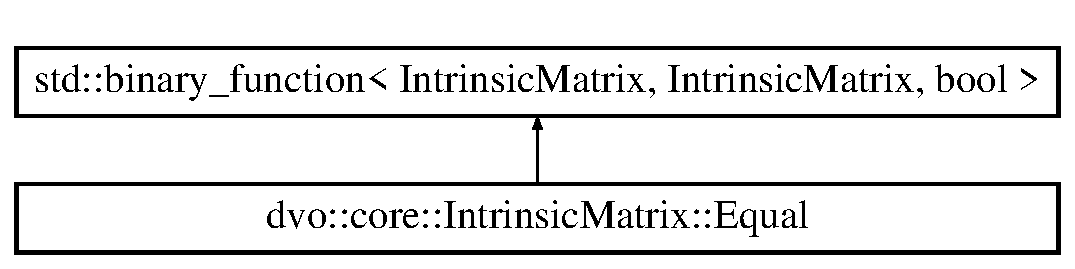
\includegraphics[height=2.000000cm]{structdvo_1_1core_1_1_intrinsic_matrix_1_1_equal}
\end{center}
\end{figure}
\subsection*{Public Member Functions}
\begin{DoxyCompactItemize}
\item 
bool \mbox{\hyperlink{structdvo_1_1core_1_1_intrinsic_matrix_1_1_equal_ab7dd89f92d6cf3f7086481e3c168fcf6}{operator()}} (\mbox{\hyperlink{structdvo_1_1core_1_1_intrinsic_matrix}{Intrinsic\+Matrix}} const \&left, \mbox{\hyperlink{structdvo_1_1core_1_1_intrinsic_matrix}{Intrinsic\+Matrix}} const \&right) const
\end{DoxyCompactItemize}


\subsection{Member Function Documentation}
\mbox{\Hypertarget{structdvo_1_1core_1_1_intrinsic_matrix_1_1_equal_ab7dd89f92d6cf3f7086481e3c168fcf6}\label{structdvo_1_1core_1_1_intrinsic_matrix_1_1_equal_ab7dd89f92d6cf3f7086481e3c168fcf6}} 
\index{dvo\+::core\+::\+Intrinsic\+Matrix\+::\+Equal@{dvo\+::core\+::\+Intrinsic\+Matrix\+::\+Equal}!operator()@{operator()}}
\index{operator()@{operator()}!dvo\+::core\+::\+Intrinsic\+Matrix\+::\+Equal@{dvo\+::core\+::\+Intrinsic\+Matrix\+::\+Equal}}
\subsubsection{\texorpdfstring{operator()()}{operator()()}}
{\footnotesize\ttfamily bool dvo\+::core\+::\+Intrinsic\+Matrix\+::\+Equal\+::operator() (\begin{DoxyParamCaption}\item[{\mbox{\hyperlink{structdvo_1_1core_1_1_intrinsic_matrix}{Intrinsic\+Matrix}} const \&}]{left,  }\item[{\mbox{\hyperlink{structdvo_1_1core_1_1_intrinsic_matrix}{Intrinsic\+Matrix}} const \&}]{right }\end{DoxyParamCaption}) const}



The documentation for this struct was generated from the following files\+:\begin{DoxyCompactItemize}
\item 
dvo\+\_\+core/include/dvo/core/\mbox{\hyperlink{intrinsic__matrix_8h}{intrinsic\+\_\+matrix.\+h}}\item 
dvo\+\_\+core/src/core/\mbox{\hyperlink{intrinsic__matrix_8cpp}{intrinsic\+\_\+matrix.\+cpp}}\end{DoxyCompactItemize}

\hypertarget{classdvo_1_1core_1_1_evd_least_squares}{}\section{dvo\+:\+:core\+:\+:Evd\+Least\+Squares Class Reference}
\label{classdvo_1_1core_1_1_evd_least_squares}\index{dvo\+::core\+::\+Evd\+Least\+Squares@{dvo\+::core\+::\+Evd\+Least\+Squares}}


{\ttfamily \#include $<$least\+\_\+squares.\+h$>$}

Inheritance diagram for dvo\+:\+:core\+:\+:Evd\+Least\+Squares\+:\begin{figure}[H]
\begin{center}
\leavevmode
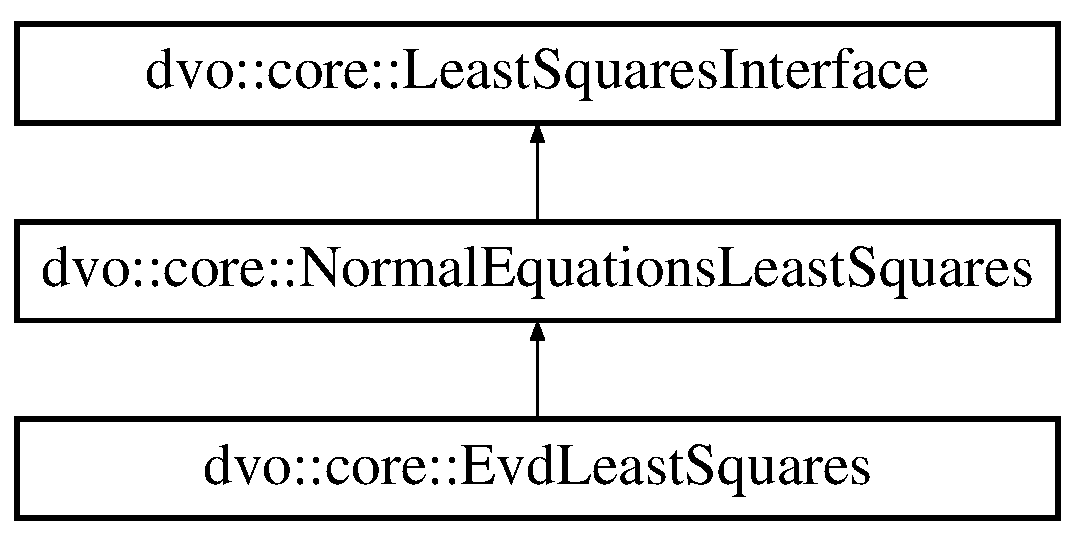
\includegraphics[height=3.000000cm]{classdvo_1_1core_1_1_evd_least_squares}
\end{center}
\end{figure}
\subsection*{Public Member Functions}
\begin{DoxyCompactItemize}
\item 
virtual \mbox{\hyperlink{classdvo_1_1core_1_1_evd_least_squares_a560024b449e22ea0da7565b5d798b154}{$\sim$\+Evd\+Least\+Squares}} ()
\item 
virtual void \mbox{\hyperlink{classdvo_1_1core_1_1_evd_least_squares_a7264139b3006d803039707c4318d2451}{solve}} (\mbox{\hyperlink{namespacedvo_1_1core_a05327f3312d32a301bce9fccda9e5807}{Vector6}} \&x)
\end{DoxyCompactItemize}
\subsection*{Additional Inherited Members}


\subsection{Detailed Description}
Same as \mbox{\hyperlink{classdvo_1_1core_1_1_normal_equations_least_squares}{Normal\+Equations\+Least\+Squares}}, but solves normal equations with Eigen\+Value\+Decomposition. 

\subsection{Constructor \& Destructor Documentation}
\mbox{\Hypertarget{classdvo_1_1core_1_1_evd_least_squares_a560024b449e22ea0da7565b5d798b154}\label{classdvo_1_1core_1_1_evd_least_squares_a560024b449e22ea0da7565b5d798b154}} 
\index{dvo\+::core\+::\+Evd\+Least\+Squares@{dvo\+::core\+::\+Evd\+Least\+Squares}!````~Evd\+Least\+Squares@{$\sim$\+Evd\+Least\+Squares}}
\index{````~Evd\+Least\+Squares@{$\sim$\+Evd\+Least\+Squares}!dvo\+::core\+::\+Evd\+Least\+Squares@{dvo\+::core\+::\+Evd\+Least\+Squares}}
\subsubsection{\texorpdfstring{$\sim$\+Evd\+Least\+Squares()}{~EvdLeastSquares()}}
{\footnotesize\ttfamily dvo\+::core\+::\+Evd\+Least\+Squares\+::$\sim$\+Evd\+Least\+Squares (\begin{DoxyParamCaption}{ }\end{DoxyParamCaption})\hspace{0.3cm}{\ttfamily [virtual]}}



\subsection{Member Function Documentation}
\mbox{\Hypertarget{classdvo_1_1core_1_1_evd_least_squares_a7264139b3006d803039707c4318d2451}\label{classdvo_1_1core_1_1_evd_least_squares_a7264139b3006d803039707c4318d2451}} 
\index{dvo\+::core\+::\+Evd\+Least\+Squares@{dvo\+::core\+::\+Evd\+Least\+Squares}!solve@{solve}}
\index{solve@{solve}!dvo\+::core\+::\+Evd\+Least\+Squares@{dvo\+::core\+::\+Evd\+Least\+Squares}}
\subsubsection{\texorpdfstring{solve()}{solve()}}
{\footnotesize\ttfamily void dvo\+::core\+::\+Evd\+Least\+Squares\+::solve (\begin{DoxyParamCaption}\item[{\mbox{\hyperlink{namespacedvo_1_1core_a05327f3312d32a301bce9fccda9e5807}{Vector6}} \&}]{x }\end{DoxyParamCaption})\hspace{0.3cm}{\ttfamily [virtual]}}



Reimplemented from \mbox{\hyperlink{classdvo_1_1core_1_1_normal_equations_least_squares_a8a25d3970f6506df2066995f2f2effda}{dvo\+::core\+::\+Normal\+Equations\+Least\+Squares}}.



The documentation for this class was generated from the following files\+:\begin{DoxyCompactItemize}
\item 
dvo\+\_\+core/include/dvo/core/\mbox{\hyperlink{least__squares_8h}{least\+\_\+squares.\+h}}\item 
dvo\+\_\+core/src/core/\mbox{\hyperlink{least__squares_8cpp}{least\+\_\+squares.\+cpp}}\end{DoxyCompactItemize}

\hypertarget{classdvo__benchmark_1_1_file_reader}{}\section{dvo\+\_\+benchmark\+:\+:File\+Reader$<$ EntryT $>$ Class Template Reference}
\label{classdvo__benchmark_1_1_file_reader}\index{dvo\+\_\+benchmark\+::\+File\+Reader$<$ Entry\+T $>$@{dvo\+\_\+benchmark\+::\+File\+Reader$<$ Entry\+T $>$}}


{\ttfamily \#include $<$file\+\_\+reader.\+h$>$}

\subsection*{Public Member Functions}
\begin{DoxyCompactItemize}
\item 
\mbox{\hyperlink{classdvo__benchmark_1_1_file_reader_a4106b3318059b0f2a8587ee1457b0472}{File\+Reader}} (std\+::string \&file)
\item 
virtual \mbox{\hyperlink{classdvo__benchmark_1_1_file_reader_a1cccea52d55942eb1cbab0ae2a856914}{$\sim$\+File\+Reader}} ()
\item 
void \mbox{\hyperlink{classdvo__benchmark_1_1_file_reader_a2f62b338f1a1b8ffd47091e769c03f8b}{skip}} (int num\+\_\+lines)
\item 
void \mbox{\hyperlink{classdvo__benchmark_1_1_file_reader_abc0efc95a5f911cf75417f7777e333f4}{skip\+Comments}} ()
\item 
bool \mbox{\hyperlink{classdvo__benchmark_1_1_file_reader_a47866d6c871158248f3521bf496084e6}{next}} ()
\item 
void \mbox{\hyperlink{classdvo__benchmark_1_1_file_reader_a886900b867b838cbf964bdd8daebb772}{read\+All\+Entries}} (std\+::vector$<$ EntryT $>$ \&entries)
\item 
\mbox{\hyperlink{classdvo__benchmark_1_1_file_reader_af0c136260af17b315ec2761dd647e5e1}{F\+I\+\_\+\+A\+T\+T\+R\+I\+B\+U\+TE}} (\mbox{\hyperlink{classdvo__benchmark_1_1_file_reader}{File\+Reader}}, EntryT, entry)
\item 
\mbox{\hyperlink{classdvo__benchmark_1_1_file_reader_ab929f48570b38a74293fae46a6dfce2d}{F\+I\+\_\+\+A\+T\+T\+R\+I\+B\+U\+TE}} (\mbox{\hyperlink{classdvo__benchmark_1_1_file_reader}{File\+Reader}}, bool, has\+Entry)
\end{DoxyCompactItemize}


\subsection{Detailed Description}
\subsubsection*{template$<$class EntryT$>$\newline
class dvo\+\_\+benchmark\+::\+File\+Reader$<$ Entry\+T $>$}

EntryT has to support the following operator std\+::istream\& operator $>$$>$(std\+::istream\&, Entry\+T\&); 

\subsection{Constructor \& Destructor Documentation}
\mbox{\Hypertarget{classdvo__benchmark_1_1_file_reader_a4106b3318059b0f2a8587ee1457b0472}\label{classdvo__benchmark_1_1_file_reader_a4106b3318059b0f2a8587ee1457b0472}} 
\index{dvo\+\_\+benchmark\+::\+File\+Reader@{dvo\+\_\+benchmark\+::\+File\+Reader}!File\+Reader@{File\+Reader}}
\index{File\+Reader@{File\+Reader}!dvo\+\_\+benchmark\+::\+File\+Reader@{dvo\+\_\+benchmark\+::\+File\+Reader}}
\subsubsection{\texorpdfstring{File\+Reader()}{FileReader()}}
{\footnotesize\ttfamily template$<$class EntryT$>$ \\
\mbox{\hyperlink{classdvo__benchmark_1_1_file_reader}{dvo\+\_\+benchmark\+::\+File\+Reader}}$<$ EntryT $>$\+::\mbox{\hyperlink{classdvo__benchmark_1_1_file_reader}{File\+Reader}} (\begin{DoxyParamCaption}\item[{std\+::string \&}]{file }\end{DoxyParamCaption})\hspace{0.3cm}{\ttfamily [inline]}}

\mbox{\Hypertarget{classdvo__benchmark_1_1_file_reader_a1cccea52d55942eb1cbab0ae2a856914}\label{classdvo__benchmark_1_1_file_reader_a1cccea52d55942eb1cbab0ae2a856914}} 
\index{dvo\+\_\+benchmark\+::\+File\+Reader@{dvo\+\_\+benchmark\+::\+File\+Reader}!````~File\+Reader@{$\sim$\+File\+Reader}}
\index{````~File\+Reader@{$\sim$\+File\+Reader}!dvo\+\_\+benchmark\+::\+File\+Reader@{dvo\+\_\+benchmark\+::\+File\+Reader}}
\subsubsection{\texorpdfstring{$\sim$\+File\+Reader()}{~FileReader()}}
{\footnotesize\ttfamily template$<$class EntryT$>$ \\
virtual \mbox{\hyperlink{classdvo__benchmark_1_1_file_reader}{dvo\+\_\+benchmark\+::\+File\+Reader}}$<$ EntryT $>$\+::$\sim$\mbox{\hyperlink{classdvo__benchmark_1_1_file_reader}{File\+Reader}} (\begin{DoxyParamCaption}{ }\end{DoxyParamCaption})\hspace{0.3cm}{\ttfamily [inline]}, {\ttfamily [virtual]}}



\subsection{Member Function Documentation}
\mbox{\Hypertarget{classdvo__benchmark_1_1_file_reader_af0c136260af17b315ec2761dd647e5e1}\label{classdvo__benchmark_1_1_file_reader_af0c136260af17b315ec2761dd647e5e1}} 
\index{dvo\+\_\+benchmark\+::\+File\+Reader@{dvo\+\_\+benchmark\+::\+File\+Reader}!F\+I\+\_\+\+A\+T\+T\+R\+I\+B\+U\+TE@{F\+I\+\_\+\+A\+T\+T\+R\+I\+B\+U\+TE}}
\index{F\+I\+\_\+\+A\+T\+T\+R\+I\+B\+U\+TE@{F\+I\+\_\+\+A\+T\+T\+R\+I\+B\+U\+TE}!dvo\+\_\+benchmark\+::\+File\+Reader@{dvo\+\_\+benchmark\+::\+File\+Reader}}
\subsubsection{\texorpdfstring{F\+I\+\_\+\+A\+T\+T\+R\+I\+B\+U\+T\+E()}{FI\_ATTRIBUTE()}\hspace{0.1cm}{\footnotesize\ttfamily [1/2]}}
{\footnotesize\ttfamily template$<$class EntryT$>$ \\
\mbox{\hyperlink{classdvo__benchmark_1_1_file_reader}{dvo\+\_\+benchmark\+::\+File\+Reader}}$<$ EntryT $>$\+::F\+I\+\_\+\+A\+T\+T\+R\+I\+B\+U\+TE (\begin{DoxyParamCaption}\item[{\mbox{\hyperlink{classdvo__benchmark_1_1_file_reader}{File\+Reader}}$<$ EntryT $>$}]{,  }\item[{EntryT}]{,  }\item[{entry}]{ }\end{DoxyParamCaption})}

Gets the current entry. \mbox{\Hypertarget{classdvo__benchmark_1_1_file_reader_ab929f48570b38a74293fae46a6dfce2d}\label{classdvo__benchmark_1_1_file_reader_ab929f48570b38a74293fae46a6dfce2d}} 
\index{dvo\+\_\+benchmark\+::\+File\+Reader@{dvo\+\_\+benchmark\+::\+File\+Reader}!F\+I\+\_\+\+A\+T\+T\+R\+I\+B\+U\+TE@{F\+I\+\_\+\+A\+T\+T\+R\+I\+B\+U\+TE}}
\index{F\+I\+\_\+\+A\+T\+T\+R\+I\+B\+U\+TE@{F\+I\+\_\+\+A\+T\+T\+R\+I\+B\+U\+TE}!dvo\+\_\+benchmark\+::\+File\+Reader@{dvo\+\_\+benchmark\+::\+File\+Reader}}
\subsubsection{\texorpdfstring{F\+I\+\_\+\+A\+T\+T\+R\+I\+B\+U\+T\+E()}{FI\_ATTRIBUTE()}\hspace{0.1cm}{\footnotesize\ttfamily [2/2]}}
{\footnotesize\ttfamily template$<$class EntryT$>$ \\
\mbox{\hyperlink{classdvo__benchmark_1_1_file_reader}{dvo\+\_\+benchmark\+::\+File\+Reader}}$<$ EntryT $>$\+::F\+I\+\_\+\+A\+T\+T\+R\+I\+B\+U\+TE (\begin{DoxyParamCaption}\item[{\mbox{\hyperlink{classdvo__benchmark_1_1_file_reader}{File\+Reader}}$<$ EntryT $>$}]{,  }\item[{bool}]{,  }\item[{has\+Entry}]{ }\end{DoxyParamCaption})}

Determines whether the first entry was read. \mbox{\Hypertarget{classdvo__benchmark_1_1_file_reader_a47866d6c871158248f3521bf496084e6}\label{classdvo__benchmark_1_1_file_reader_a47866d6c871158248f3521bf496084e6}} 
\index{dvo\+\_\+benchmark\+::\+File\+Reader@{dvo\+\_\+benchmark\+::\+File\+Reader}!next@{next}}
\index{next@{next}!dvo\+\_\+benchmark\+::\+File\+Reader@{dvo\+\_\+benchmark\+::\+File\+Reader}}
\subsubsection{\texorpdfstring{next()}{next()}}
{\footnotesize\ttfamily template$<$class EntryT$>$ \\
bool \mbox{\hyperlink{classdvo__benchmark_1_1_file_reader}{dvo\+\_\+benchmark\+::\+File\+Reader}}$<$ EntryT $>$\+::next (\begin{DoxyParamCaption}{ }\end{DoxyParamCaption})\hspace{0.3cm}{\ttfamily [inline]}}

Moves to the next entry in the file. Returns true, if there was a next entry, false otherwise. \mbox{\Hypertarget{classdvo__benchmark_1_1_file_reader_a886900b867b838cbf964bdd8daebb772}\label{classdvo__benchmark_1_1_file_reader_a886900b867b838cbf964bdd8daebb772}} 
\index{dvo\+\_\+benchmark\+::\+File\+Reader@{dvo\+\_\+benchmark\+::\+File\+Reader}!read\+All\+Entries@{read\+All\+Entries}}
\index{read\+All\+Entries@{read\+All\+Entries}!dvo\+\_\+benchmark\+::\+File\+Reader@{dvo\+\_\+benchmark\+::\+File\+Reader}}
\subsubsection{\texorpdfstring{read\+All\+Entries()}{readAllEntries()}}
{\footnotesize\ttfamily template$<$class EntryT$>$ \\
void \mbox{\hyperlink{classdvo__benchmark_1_1_file_reader}{dvo\+\_\+benchmark\+::\+File\+Reader}}$<$ EntryT $>$\+::read\+All\+Entries (\begin{DoxyParamCaption}\item[{std\+::vector$<$ EntryT $>$ \&}]{entries }\end{DoxyParamCaption})\hspace{0.3cm}{\ttfamily [inline]}}

Read all entries at once. \mbox{\Hypertarget{classdvo__benchmark_1_1_file_reader_a2f62b338f1a1b8ffd47091e769c03f8b}\label{classdvo__benchmark_1_1_file_reader_a2f62b338f1a1b8ffd47091e769c03f8b}} 
\index{dvo\+\_\+benchmark\+::\+File\+Reader@{dvo\+\_\+benchmark\+::\+File\+Reader}!skip@{skip}}
\index{skip@{skip}!dvo\+\_\+benchmark\+::\+File\+Reader@{dvo\+\_\+benchmark\+::\+File\+Reader}}
\subsubsection{\texorpdfstring{skip()}{skip()}}
{\footnotesize\ttfamily template$<$class EntryT$>$ \\
void \mbox{\hyperlink{classdvo__benchmark_1_1_file_reader}{dvo\+\_\+benchmark\+::\+File\+Reader}}$<$ EntryT $>$\+::skip (\begin{DoxyParamCaption}\item[{int}]{num\+\_\+lines }\end{DoxyParamCaption})\hspace{0.3cm}{\ttfamily [inline]}}

\mbox{\Hypertarget{classdvo__benchmark_1_1_file_reader_abc0efc95a5f911cf75417f7777e333f4}\label{classdvo__benchmark_1_1_file_reader_abc0efc95a5f911cf75417f7777e333f4}} 
\index{dvo\+\_\+benchmark\+::\+File\+Reader@{dvo\+\_\+benchmark\+::\+File\+Reader}!skip\+Comments@{skip\+Comments}}
\index{skip\+Comments@{skip\+Comments}!dvo\+\_\+benchmark\+::\+File\+Reader@{dvo\+\_\+benchmark\+::\+File\+Reader}}
\subsubsection{\texorpdfstring{skip\+Comments()}{skipComments()}}
{\footnotesize\ttfamily template$<$class EntryT$>$ \\
void \mbox{\hyperlink{classdvo__benchmark_1_1_file_reader}{dvo\+\_\+benchmark\+::\+File\+Reader}}$<$ EntryT $>$\+::skip\+Comments (\begin{DoxyParamCaption}{ }\end{DoxyParamCaption})\hspace{0.3cm}{\ttfamily [inline]}}



The documentation for this class was generated from the following file\+:\begin{DoxyCompactItemize}
\item 
dvo\+\_\+benchmark/include/dvo\+\_\+benchmark/\mbox{\hyperlink{file__reader_8h}{file\+\_\+reader.\+h}}\end{DoxyCompactItemize}

\hypertarget{classdvo__benchmark_1_1_groundtruth}{}\section{dvo\+\_\+benchmark\+:\+:Groundtruth Class Reference}
\label{classdvo__benchmark_1_1_groundtruth}\index{dvo\+\_\+benchmark\+::\+Groundtruth@{dvo\+\_\+benchmark\+::\+Groundtruth}}


{\ttfamily \#include $<$groundtruth.\+h$>$}

\subsection*{Public Member Functions}
\begin{DoxyCompactItemize}
\item 
\mbox{\hyperlink{classdvo__benchmark_1_1_groundtruth_adb2acf16f7f0a87f92db5e74876e4f2e}{Groundtruth}} ()
\item 
virtual \mbox{\hyperlink{classdvo__benchmark_1_1_groundtruth_a650239cd5e1ca8fa434e5121e7c4d727}{$\sim$\+Groundtruth}} ()
\item 
\mbox{\hyperlink{classdvo__benchmark_1_1_groundtruth_a8c504fb35eeba591d8ca830223081e1b}{F\+I\+\_\+\+A\+T\+T\+R\+I\+B\+U\+TE}} (\mbox{\hyperlink{classdvo__benchmark_1_1_groundtruth}{Groundtruth}}, ros\+::\+Time, Timestamp)
\item 
\mbox{\hyperlink{classdvo__benchmark_1_1_groundtruth_ab8ed989b9db899b7718bdb291eb18d30}{F\+I\+\_\+\+A\+T\+T\+R\+I\+B\+U\+TE}} (\mbox{\hyperlink{classdvo__benchmark_1_1_groundtruth}{Groundtruth}}, double, PositionX)
\item 
\mbox{\hyperlink{classdvo__benchmark_1_1_groundtruth_a524307c4f6c2cad806dfe36f777b7ce1}{F\+I\+\_\+\+A\+T\+T\+R\+I\+B\+U\+TE}} (\mbox{\hyperlink{classdvo__benchmark_1_1_groundtruth}{Groundtruth}}, double, PositionY)
\item 
\mbox{\hyperlink{classdvo__benchmark_1_1_groundtruth_a5775b082016a04d4a36c94e635eebfde}{F\+I\+\_\+\+A\+T\+T\+R\+I\+B\+U\+TE}} (\mbox{\hyperlink{classdvo__benchmark_1_1_groundtruth}{Groundtruth}}, double, PositionZ)
\item 
\mbox{\hyperlink{classdvo__benchmark_1_1_groundtruth_abf20e8ba0f0f6dee57f7b75f33ebec31}{F\+I\+\_\+\+A\+T\+T\+R\+I\+B\+U\+TE}} (\mbox{\hyperlink{classdvo__benchmark_1_1_groundtruth}{Groundtruth}}, double, OrientationX)
\item 
\mbox{\hyperlink{classdvo__benchmark_1_1_groundtruth_a3459d282fe7b5814c99bccfcfb6f3fd9}{F\+I\+\_\+\+A\+T\+T\+R\+I\+B\+U\+TE}} (\mbox{\hyperlink{classdvo__benchmark_1_1_groundtruth}{Groundtruth}}, double, OrientationY)
\item 
\mbox{\hyperlink{classdvo__benchmark_1_1_groundtruth_a1455c5f99d9e4426b4c74f95601ad1a8}{F\+I\+\_\+\+A\+T\+T\+R\+I\+B\+U\+TE}} (\mbox{\hyperlink{classdvo__benchmark_1_1_groundtruth}{Groundtruth}}, double, OrientationZ)
\item 
\mbox{\hyperlink{classdvo__benchmark_1_1_groundtruth_ae6d3747350b8a343c26ccd1a886ac600}{F\+I\+\_\+\+A\+T\+T\+R\+I\+B\+U\+TE}} (\mbox{\hyperlink{classdvo__benchmark_1_1_groundtruth}{Groundtruth}}, double, OrientationW)
\end{DoxyCompactItemize}
\subsection*{Friends}
\begin{DoxyCompactItemize}
\item 
std\+::ostream \& \mbox{\hyperlink{classdvo__benchmark_1_1_groundtruth_a253b88524b96be5898ba1b657cda2f9a}{operator$<$$<$}} (std\+::ostream \&out, const \mbox{\hyperlink{classdvo__benchmark_1_1_groundtruth}{Groundtruth}} \&pair)
\item 
std\+::istream \& \mbox{\hyperlink{classdvo__benchmark_1_1_groundtruth_a2ce119ce35748a3d57ec0d36499c44e1}{operator$>$$>$}} (std\+::istream \&in, \mbox{\hyperlink{classdvo__benchmark_1_1_groundtruth}{Groundtruth}} \&pair)
\end{DoxyCompactItemize}


\subsection{Constructor \& Destructor Documentation}
\mbox{\Hypertarget{classdvo__benchmark_1_1_groundtruth_adb2acf16f7f0a87f92db5e74876e4f2e}\label{classdvo__benchmark_1_1_groundtruth_adb2acf16f7f0a87f92db5e74876e4f2e}} 
\index{dvo\+\_\+benchmark\+::\+Groundtruth@{dvo\+\_\+benchmark\+::\+Groundtruth}!Groundtruth@{Groundtruth}}
\index{Groundtruth@{Groundtruth}!dvo\+\_\+benchmark\+::\+Groundtruth@{dvo\+\_\+benchmark\+::\+Groundtruth}}
\subsubsection{\texorpdfstring{Groundtruth()}{Groundtruth()}}
{\footnotesize\ttfamily dvo\+\_\+benchmark\+::\+Groundtruth\+::\+Groundtruth (\begin{DoxyParamCaption}{ }\end{DoxyParamCaption})\hspace{0.3cm}{\ttfamily [inline]}}

\mbox{\Hypertarget{classdvo__benchmark_1_1_groundtruth_a650239cd5e1ca8fa434e5121e7c4d727}\label{classdvo__benchmark_1_1_groundtruth_a650239cd5e1ca8fa434e5121e7c4d727}} 
\index{dvo\+\_\+benchmark\+::\+Groundtruth@{dvo\+\_\+benchmark\+::\+Groundtruth}!````~Groundtruth@{$\sim$\+Groundtruth}}
\index{````~Groundtruth@{$\sim$\+Groundtruth}!dvo\+\_\+benchmark\+::\+Groundtruth@{dvo\+\_\+benchmark\+::\+Groundtruth}}
\subsubsection{\texorpdfstring{$\sim$\+Groundtruth()}{~Groundtruth()}}
{\footnotesize\ttfamily virtual dvo\+\_\+benchmark\+::\+Groundtruth\+::$\sim$\+Groundtruth (\begin{DoxyParamCaption}{ }\end{DoxyParamCaption})\hspace{0.3cm}{\ttfamily [inline]}, {\ttfamily [virtual]}}



\subsection{Member Function Documentation}
\mbox{\Hypertarget{classdvo__benchmark_1_1_groundtruth_a8c504fb35eeba591d8ca830223081e1b}\label{classdvo__benchmark_1_1_groundtruth_a8c504fb35eeba591d8ca830223081e1b}} 
\index{dvo\+\_\+benchmark\+::\+Groundtruth@{dvo\+\_\+benchmark\+::\+Groundtruth}!F\+I\+\_\+\+A\+T\+T\+R\+I\+B\+U\+TE@{F\+I\+\_\+\+A\+T\+T\+R\+I\+B\+U\+TE}}
\index{F\+I\+\_\+\+A\+T\+T\+R\+I\+B\+U\+TE@{F\+I\+\_\+\+A\+T\+T\+R\+I\+B\+U\+TE}!dvo\+\_\+benchmark\+::\+Groundtruth@{dvo\+\_\+benchmark\+::\+Groundtruth}}
\subsubsection{\texorpdfstring{F\+I\+\_\+\+A\+T\+T\+R\+I\+B\+U\+T\+E()}{FI\_ATTRIBUTE()}\hspace{0.1cm}{\footnotesize\ttfamily [1/8]}}
{\footnotesize\ttfamily dvo\+\_\+benchmark\+::\+Groundtruth\+::\+F\+I\+\_\+\+A\+T\+T\+R\+I\+B\+U\+TE (\begin{DoxyParamCaption}\item[{\mbox{\hyperlink{classdvo__benchmark_1_1_groundtruth}{Groundtruth}}}]{,  }\item[{ros\+::\+Time}]{,  }\item[{Timestamp}]{ }\end{DoxyParamCaption})}

\mbox{\Hypertarget{classdvo__benchmark_1_1_groundtruth_ab8ed989b9db899b7718bdb291eb18d30}\label{classdvo__benchmark_1_1_groundtruth_ab8ed989b9db899b7718bdb291eb18d30}} 
\index{dvo\+\_\+benchmark\+::\+Groundtruth@{dvo\+\_\+benchmark\+::\+Groundtruth}!F\+I\+\_\+\+A\+T\+T\+R\+I\+B\+U\+TE@{F\+I\+\_\+\+A\+T\+T\+R\+I\+B\+U\+TE}}
\index{F\+I\+\_\+\+A\+T\+T\+R\+I\+B\+U\+TE@{F\+I\+\_\+\+A\+T\+T\+R\+I\+B\+U\+TE}!dvo\+\_\+benchmark\+::\+Groundtruth@{dvo\+\_\+benchmark\+::\+Groundtruth}}
\subsubsection{\texorpdfstring{F\+I\+\_\+\+A\+T\+T\+R\+I\+B\+U\+T\+E()}{FI\_ATTRIBUTE()}\hspace{0.1cm}{\footnotesize\ttfamily [2/8]}}
{\footnotesize\ttfamily dvo\+\_\+benchmark\+::\+Groundtruth\+::\+F\+I\+\_\+\+A\+T\+T\+R\+I\+B\+U\+TE (\begin{DoxyParamCaption}\item[{\mbox{\hyperlink{classdvo__benchmark_1_1_groundtruth}{Groundtruth}}}]{,  }\item[{double}]{,  }\item[{PositionX}]{ }\end{DoxyParamCaption})}

\mbox{\Hypertarget{classdvo__benchmark_1_1_groundtruth_a524307c4f6c2cad806dfe36f777b7ce1}\label{classdvo__benchmark_1_1_groundtruth_a524307c4f6c2cad806dfe36f777b7ce1}} 
\index{dvo\+\_\+benchmark\+::\+Groundtruth@{dvo\+\_\+benchmark\+::\+Groundtruth}!F\+I\+\_\+\+A\+T\+T\+R\+I\+B\+U\+TE@{F\+I\+\_\+\+A\+T\+T\+R\+I\+B\+U\+TE}}
\index{F\+I\+\_\+\+A\+T\+T\+R\+I\+B\+U\+TE@{F\+I\+\_\+\+A\+T\+T\+R\+I\+B\+U\+TE}!dvo\+\_\+benchmark\+::\+Groundtruth@{dvo\+\_\+benchmark\+::\+Groundtruth}}
\subsubsection{\texorpdfstring{F\+I\+\_\+\+A\+T\+T\+R\+I\+B\+U\+T\+E()}{FI\_ATTRIBUTE()}\hspace{0.1cm}{\footnotesize\ttfamily [3/8]}}
{\footnotesize\ttfamily dvo\+\_\+benchmark\+::\+Groundtruth\+::\+F\+I\+\_\+\+A\+T\+T\+R\+I\+B\+U\+TE (\begin{DoxyParamCaption}\item[{\mbox{\hyperlink{classdvo__benchmark_1_1_groundtruth}{Groundtruth}}}]{,  }\item[{double}]{,  }\item[{PositionY}]{ }\end{DoxyParamCaption})}

\mbox{\Hypertarget{classdvo__benchmark_1_1_groundtruth_a5775b082016a04d4a36c94e635eebfde}\label{classdvo__benchmark_1_1_groundtruth_a5775b082016a04d4a36c94e635eebfde}} 
\index{dvo\+\_\+benchmark\+::\+Groundtruth@{dvo\+\_\+benchmark\+::\+Groundtruth}!F\+I\+\_\+\+A\+T\+T\+R\+I\+B\+U\+TE@{F\+I\+\_\+\+A\+T\+T\+R\+I\+B\+U\+TE}}
\index{F\+I\+\_\+\+A\+T\+T\+R\+I\+B\+U\+TE@{F\+I\+\_\+\+A\+T\+T\+R\+I\+B\+U\+TE}!dvo\+\_\+benchmark\+::\+Groundtruth@{dvo\+\_\+benchmark\+::\+Groundtruth}}
\subsubsection{\texorpdfstring{F\+I\+\_\+\+A\+T\+T\+R\+I\+B\+U\+T\+E()}{FI\_ATTRIBUTE()}\hspace{0.1cm}{\footnotesize\ttfamily [4/8]}}
{\footnotesize\ttfamily dvo\+\_\+benchmark\+::\+Groundtruth\+::\+F\+I\+\_\+\+A\+T\+T\+R\+I\+B\+U\+TE (\begin{DoxyParamCaption}\item[{\mbox{\hyperlink{classdvo__benchmark_1_1_groundtruth}{Groundtruth}}}]{,  }\item[{double}]{,  }\item[{PositionZ}]{ }\end{DoxyParamCaption})}

\mbox{\Hypertarget{classdvo__benchmark_1_1_groundtruth_abf20e8ba0f0f6dee57f7b75f33ebec31}\label{classdvo__benchmark_1_1_groundtruth_abf20e8ba0f0f6dee57f7b75f33ebec31}} 
\index{dvo\+\_\+benchmark\+::\+Groundtruth@{dvo\+\_\+benchmark\+::\+Groundtruth}!F\+I\+\_\+\+A\+T\+T\+R\+I\+B\+U\+TE@{F\+I\+\_\+\+A\+T\+T\+R\+I\+B\+U\+TE}}
\index{F\+I\+\_\+\+A\+T\+T\+R\+I\+B\+U\+TE@{F\+I\+\_\+\+A\+T\+T\+R\+I\+B\+U\+TE}!dvo\+\_\+benchmark\+::\+Groundtruth@{dvo\+\_\+benchmark\+::\+Groundtruth}}
\subsubsection{\texorpdfstring{F\+I\+\_\+\+A\+T\+T\+R\+I\+B\+U\+T\+E()}{FI\_ATTRIBUTE()}\hspace{0.1cm}{\footnotesize\ttfamily [5/8]}}
{\footnotesize\ttfamily dvo\+\_\+benchmark\+::\+Groundtruth\+::\+F\+I\+\_\+\+A\+T\+T\+R\+I\+B\+U\+TE (\begin{DoxyParamCaption}\item[{\mbox{\hyperlink{classdvo__benchmark_1_1_groundtruth}{Groundtruth}}}]{,  }\item[{double}]{,  }\item[{OrientationX}]{ }\end{DoxyParamCaption})}

\mbox{\Hypertarget{classdvo__benchmark_1_1_groundtruth_a3459d282fe7b5814c99bccfcfb6f3fd9}\label{classdvo__benchmark_1_1_groundtruth_a3459d282fe7b5814c99bccfcfb6f3fd9}} 
\index{dvo\+\_\+benchmark\+::\+Groundtruth@{dvo\+\_\+benchmark\+::\+Groundtruth}!F\+I\+\_\+\+A\+T\+T\+R\+I\+B\+U\+TE@{F\+I\+\_\+\+A\+T\+T\+R\+I\+B\+U\+TE}}
\index{F\+I\+\_\+\+A\+T\+T\+R\+I\+B\+U\+TE@{F\+I\+\_\+\+A\+T\+T\+R\+I\+B\+U\+TE}!dvo\+\_\+benchmark\+::\+Groundtruth@{dvo\+\_\+benchmark\+::\+Groundtruth}}
\subsubsection{\texorpdfstring{F\+I\+\_\+\+A\+T\+T\+R\+I\+B\+U\+T\+E()}{FI\_ATTRIBUTE()}\hspace{0.1cm}{\footnotesize\ttfamily [6/8]}}
{\footnotesize\ttfamily dvo\+\_\+benchmark\+::\+Groundtruth\+::\+F\+I\+\_\+\+A\+T\+T\+R\+I\+B\+U\+TE (\begin{DoxyParamCaption}\item[{\mbox{\hyperlink{classdvo__benchmark_1_1_groundtruth}{Groundtruth}}}]{,  }\item[{double}]{,  }\item[{OrientationY}]{ }\end{DoxyParamCaption})}

\mbox{\Hypertarget{classdvo__benchmark_1_1_groundtruth_a1455c5f99d9e4426b4c74f95601ad1a8}\label{classdvo__benchmark_1_1_groundtruth_a1455c5f99d9e4426b4c74f95601ad1a8}} 
\index{dvo\+\_\+benchmark\+::\+Groundtruth@{dvo\+\_\+benchmark\+::\+Groundtruth}!F\+I\+\_\+\+A\+T\+T\+R\+I\+B\+U\+TE@{F\+I\+\_\+\+A\+T\+T\+R\+I\+B\+U\+TE}}
\index{F\+I\+\_\+\+A\+T\+T\+R\+I\+B\+U\+TE@{F\+I\+\_\+\+A\+T\+T\+R\+I\+B\+U\+TE}!dvo\+\_\+benchmark\+::\+Groundtruth@{dvo\+\_\+benchmark\+::\+Groundtruth}}
\subsubsection{\texorpdfstring{F\+I\+\_\+\+A\+T\+T\+R\+I\+B\+U\+T\+E()}{FI\_ATTRIBUTE()}\hspace{0.1cm}{\footnotesize\ttfamily [7/8]}}
{\footnotesize\ttfamily dvo\+\_\+benchmark\+::\+Groundtruth\+::\+F\+I\+\_\+\+A\+T\+T\+R\+I\+B\+U\+TE (\begin{DoxyParamCaption}\item[{\mbox{\hyperlink{classdvo__benchmark_1_1_groundtruth}{Groundtruth}}}]{,  }\item[{double}]{,  }\item[{OrientationZ}]{ }\end{DoxyParamCaption})}

\mbox{\Hypertarget{classdvo__benchmark_1_1_groundtruth_ae6d3747350b8a343c26ccd1a886ac600}\label{classdvo__benchmark_1_1_groundtruth_ae6d3747350b8a343c26ccd1a886ac600}} 
\index{dvo\+\_\+benchmark\+::\+Groundtruth@{dvo\+\_\+benchmark\+::\+Groundtruth}!F\+I\+\_\+\+A\+T\+T\+R\+I\+B\+U\+TE@{F\+I\+\_\+\+A\+T\+T\+R\+I\+B\+U\+TE}}
\index{F\+I\+\_\+\+A\+T\+T\+R\+I\+B\+U\+TE@{F\+I\+\_\+\+A\+T\+T\+R\+I\+B\+U\+TE}!dvo\+\_\+benchmark\+::\+Groundtruth@{dvo\+\_\+benchmark\+::\+Groundtruth}}
\subsubsection{\texorpdfstring{F\+I\+\_\+\+A\+T\+T\+R\+I\+B\+U\+T\+E()}{FI\_ATTRIBUTE()}\hspace{0.1cm}{\footnotesize\ttfamily [8/8]}}
{\footnotesize\ttfamily dvo\+\_\+benchmark\+::\+Groundtruth\+::\+F\+I\+\_\+\+A\+T\+T\+R\+I\+B\+U\+TE (\begin{DoxyParamCaption}\item[{\mbox{\hyperlink{classdvo__benchmark_1_1_groundtruth}{Groundtruth}}}]{,  }\item[{double}]{,  }\item[{OrientationW}]{ }\end{DoxyParamCaption})}



\subsection{Friends And Related Function Documentation}
\mbox{\Hypertarget{classdvo__benchmark_1_1_groundtruth_a253b88524b96be5898ba1b657cda2f9a}\label{classdvo__benchmark_1_1_groundtruth_a253b88524b96be5898ba1b657cda2f9a}} 
\index{dvo\+\_\+benchmark\+::\+Groundtruth@{dvo\+\_\+benchmark\+::\+Groundtruth}!operator$<$$<$@{operator$<$$<$}}
\index{operator$<$$<$@{operator$<$$<$}!dvo\+\_\+benchmark\+::\+Groundtruth@{dvo\+\_\+benchmark\+::\+Groundtruth}}
\subsubsection{\texorpdfstring{operator$<$$<$}{operator<<}}
{\footnotesize\ttfamily std\+::ostream\& operator$<$$<$ (\begin{DoxyParamCaption}\item[{std\+::ostream \&}]{out,  }\item[{const \mbox{\hyperlink{classdvo__benchmark_1_1_groundtruth}{Groundtruth}} \&}]{pair }\end{DoxyParamCaption})\hspace{0.3cm}{\ttfamily [friend]}}

\mbox{\Hypertarget{classdvo__benchmark_1_1_groundtruth_a2ce119ce35748a3d57ec0d36499c44e1}\label{classdvo__benchmark_1_1_groundtruth_a2ce119ce35748a3d57ec0d36499c44e1}} 
\index{dvo\+\_\+benchmark\+::\+Groundtruth@{dvo\+\_\+benchmark\+::\+Groundtruth}!operator$>$$>$@{operator$>$$>$}}
\index{operator$>$$>$@{operator$>$$>$}!dvo\+\_\+benchmark\+::\+Groundtruth@{dvo\+\_\+benchmark\+::\+Groundtruth}}
\subsubsection{\texorpdfstring{operator$>$$>$}{operator>>}}
{\footnotesize\ttfamily std\+::istream\& operator$>$$>$ (\begin{DoxyParamCaption}\item[{std\+::istream \&}]{in,  }\item[{\mbox{\hyperlink{classdvo__benchmark_1_1_groundtruth}{Groundtruth}} \&}]{pair }\end{DoxyParamCaption})\hspace{0.3cm}{\ttfamily [friend]}}



The documentation for this class was generated from the following file\+:\begin{DoxyCompactItemize}
\item 
dvo\+\_\+benchmark/include/dvo\+\_\+benchmark/\mbox{\hyperlink{groundtruth_8h}{groundtruth.\+h}}\end{DoxyCompactItemize}

\hypertarget{structdvo_1_1core_1_1_intrinsic_matrix_1_1_hash}{}\section{dvo\+:\+:core\+:\+:Intrinsic\+Matrix\+:\+:Hash Struct Reference}
\label{structdvo_1_1core_1_1_intrinsic_matrix_1_1_hash}\index{dvo\+::core\+::\+Intrinsic\+Matrix\+::\+Hash@{dvo\+::core\+::\+Intrinsic\+Matrix\+::\+Hash}}


{\ttfamily \#include $<$intrinsic\+\_\+matrix.\+h$>$}

Inheritance diagram for dvo\+:\+:core\+:\+:Intrinsic\+Matrix\+:\+:Hash\+:\begin{figure}[H]
\begin{center}
\leavevmode
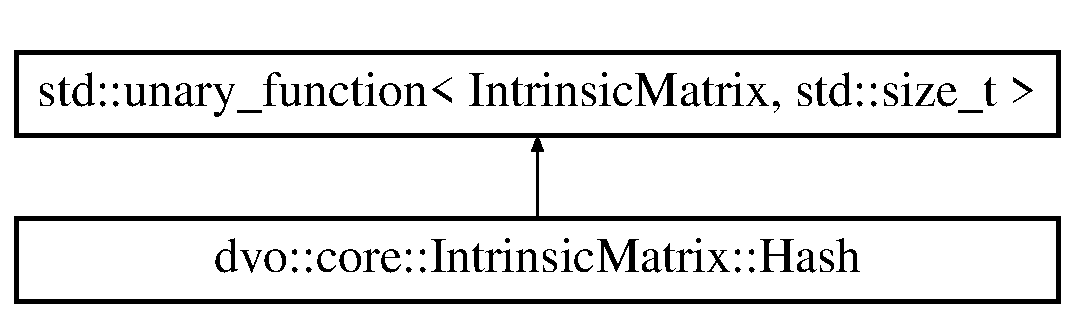
\includegraphics[height=2.000000cm]{structdvo_1_1core_1_1_intrinsic_matrix_1_1_hash}
\end{center}
\end{figure}
\subsection*{Public Member Functions}
\begin{DoxyCompactItemize}
\item 
std\+::size\+\_\+t \mbox{\hyperlink{structdvo_1_1core_1_1_intrinsic_matrix_1_1_hash_a1618ad126d9e78c43c51d9e87dbb6973}{operator()}} (\mbox{\hyperlink{structdvo_1_1core_1_1_intrinsic_matrix}{Intrinsic\+Matrix}} const \&value) const
\end{DoxyCompactItemize}


\subsection{Member Function Documentation}
\mbox{\Hypertarget{structdvo_1_1core_1_1_intrinsic_matrix_1_1_hash_a1618ad126d9e78c43c51d9e87dbb6973}\label{structdvo_1_1core_1_1_intrinsic_matrix_1_1_hash_a1618ad126d9e78c43c51d9e87dbb6973}} 
\index{dvo\+::core\+::\+Intrinsic\+Matrix\+::\+Hash@{dvo\+::core\+::\+Intrinsic\+Matrix\+::\+Hash}!operator()@{operator()}}
\index{operator()@{operator()}!dvo\+::core\+::\+Intrinsic\+Matrix\+::\+Hash@{dvo\+::core\+::\+Intrinsic\+Matrix\+::\+Hash}}
\subsubsection{\texorpdfstring{operator()()}{operator()()}}
{\footnotesize\ttfamily std\+::size\+\_\+t dvo\+::core\+::\+Intrinsic\+Matrix\+::\+Hash\+::operator() (\begin{DoxyParamCaption}\item[{\mbox{\hyperlink{structdvo_1_1core_1_1_intrinsic_matrix}{Intrinsic\+Matrix}} const \&}]{value }\end{DoxyParamCaption}) const}



The documentation for this struct was generated from the following files\+:\begin{DoxyCompactItemize}
\item 
dvo\+\_\+core/include/dvo/core/\mbox{\hyperlink{intrinsic__matrix_8h}{intrinsic\+\_\+matrix.\+h}}\item 
dvo\+\_\+core/src/core/\mbox{\hyperlink{intrinsic__matrix_8cpp}{intrinsic\+\_\+matrix.\+cpp}}\end{DoxyCompactItemize}

\hypertarget{classdvo_1_1core_1_1_huber_influence_function}{}\section{dvo\+:\+:core\+:\+:Huber\+Influence\+Function Class Reference}
\label{classdvo_1_1core_1_1_huber_influence_function}\index{dvo\+::core\+::\+Huber\+Influence\+Function@{dvo\+::core\+::\+Huber\+Influence\+Function}}


{\ttfamily \#include $<$weight\+\_\+calculation.\+h$>$}

Inheritance diagram for dvo\+:\+:core\+:\+:Huber\+Influence\+Function\+:\begin{figure}[H]
\begin{center}
\leavevmode
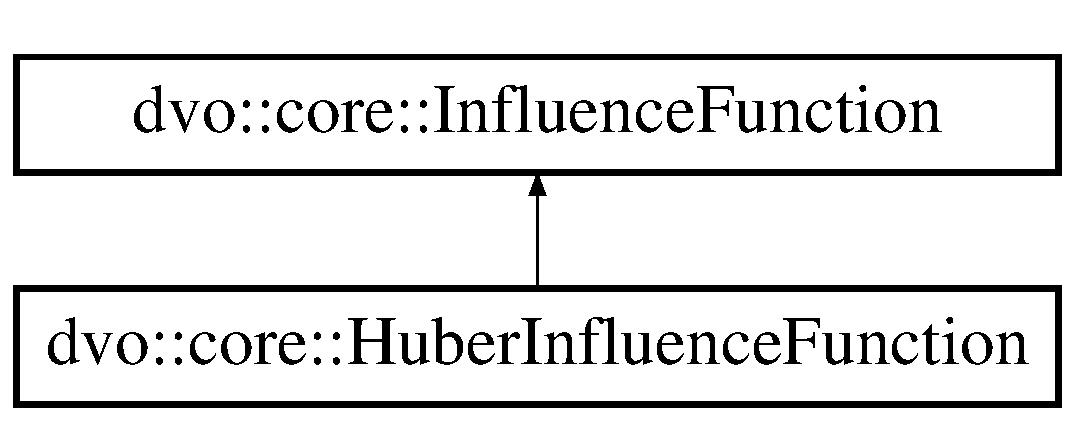
\includegraphics[height=2.000000cm]{classdvo_1_1core_1_1_huber_influence_function}
\end{center}
\end{figure}
\subsection*{Public Member Functions}
\begin{DoxyCompactItemize}
\item 
\mbox{\hyperlink{classdvo_1_1core_1_1_huber_influence_function_aa881a4af638bdc2ecc8ca2b653f4a04b}{Huber\+Influence\+Function}} (const float k=\mbox{\hyperlink{classdvo_1_1core_1_1_huber_influence_function_a7298db77700e394a56fafbf20da229fc}{D\+E\+F\+A\+U\+L\+T\+\_\+K}})
\item 
virtual \mbox{\hyperlink{classdvo_1_1core_1_1_huber_influence_function_ab243ee7b88189c9232372e316179f111}{$\sim$\+Huber\+Influence\+Function}} ()
\item 
virtual float \mbox{\hyperlink{classdvo_1_1core_1_1_huber_influence_function_af41e9e57eedcd25db690a1f41f3d6c8a}{value}} (const float \&x) const
\item 
virtual void \mbox{\hyperlink{classdvo_1_1core_1_1_huber_influence_function_aab5a25ad6f632e829c8ad2ccf073fdec}{configure}} (const float \&param)
\end{DoxyCompactItemize}
\subsection*{Static Public Attributes}
\begin{DoxyCompactItemize}
\item 
static const float \mbox{\hyperlink{classdvo_1_1core_1_1_huber_influence_function_a7298db77700e394a56fafbf20da229fc}{D\+E\+F\+A\+U\+L\+T\+\_\+K}} = 1.\+345f
\end{DoxyCompactItemize}


\subsection{Constructor \& Destructor Documentation}
\mbox{\Hypertarget{classdvo_1_1core_1_1_huber_influence_function_aa881a4af638bdc2ecc8ca2b653f4a04b}\label{classdvo_1_1core_1_1_huber_influence_function_aa881a4af638bdc2ecc8ca2b653f4a04b}} 
\index{dvo\+::core\+::\+Huber\+Influence\+Function@{dvo\+::core\+::\+Huber\+Influence\+Function}!Huber\+Influence\+Function@{Huber\+Influence\+Function}}
\index{Huber\+Influence\+Function@{Huber\+Influence\+Function}!dvo\+::core\+::\+Huber\+Influence\+Function@{dvo\+::core\+::\+Huber\+Influence\+Function}}
\subsubsection{\texorpdfstring{Huber\+Influence\+Function()}{HuberInfluenceFunction()}}
{\footnotesize\ttfamily dvo\+::core\+::\+Huber\+Influence\+Function\+::\+Huber\+Influence\+Function (\begin{DoxyParamCaption}\item[{const float}]{k = {\ttfamily \mbox{\hyperlink{classdvo_1_1core_1_1_huber_influence_function_a7298db77700e394a56fafbf20da229fc}{D\+E\+F\+A\+U\+L\+T\+\_\+K}}} }\end{DoxyParamCaption})}

\mbox{\Hypertarget{classdvo_1_1core_1_1_huber_influence_function_ab243ee7b88189c9232372e316179f111}\label{classdvo_1_1core_1_1_huber_influence_function_ab243ee7b88189c9232372e316179f111}} 
\index{dvo\+::core\+::\+Huber\+Influence\+Function@{dvo\+::core\+::\+Huber\+Influence\+Function}!````~Huber\+Influence\+Function@{$\sim$\+Huber\+Influence\+Function}}
\index{````~Huber\+Influence\+Function@{$\sim$\+Huber\+Influence\+Function}!dvo\+::core\+::\+Huber\+Influence\+Function@{dvo\+::core\+::\+Huber\+Influence\+Function}}
\subsubsection{\texorpdfstring{$\sim$\+Huber\+Influence\+Function()}{~HuberInfluenceFunction()}}
{\footnotesize\ttfamily virtual dvo\+::core\+::\+Huber\+Influence\+Function\+::$\sim$\+Huber\+Influence\+Function (\begin{DoxyParamCaption}{ }\end{DoxyParamCaption})\hspace{0.3cm}{\ttfamily [inline]}, {\ttfamily [virtual]}}



\subsection{Member Function Documentation}
\mbox{\Hypertarget{classdvo_1_1core_1_1_huber_influence_function_aab5a25ad6f632e829c8ad2ccf073fdec}\label{classdvo_1_1core_1_1_huber_influence_function_aab5a25ad6f632e829c8ad2ccf073fdec}} 
\index{dvo\+::core\+::\+Huber\+Influence\+Function@{dvo\+::core\+::\+Huber\+Influence\+Function}!configure@{configure}}
\index{configure@{configure}!dvo\+::core\+::\+Huber\+Influence\+Function@{dvo\+::core\+::\+Huber\+Influence\+Function}}
\subsubsection{\texorpdfstring{configure()}{configure()}}
{\footnotesize\ttfamily void dvo\+::core\+::\+Huber\+Influence\+Function\+::configure (\begin{DoxyParamCaption}\item[{const float \&}]{param }\end{DoxyParamCaption})\hspace{0.3cm}{\ttfamily [virtual]}}



Reimplemented from \mbox{\hyperlink{classdvo_1_1core_1_1_influence_function_a4773b03ca609bc5d8391d09d92ab34ad}{dvo\+::core\+::\+Influence\+Function}}.

\mbox{\Hypertarget{classdvo_1_1core_1_1_huber_influence_function_af41e9e57eedcd25db690a1f41f3d6c8a}\label{classdvo_1_1core_1_1_huber_influence_function_af41e9e57eedcd25db690a1f41f3d6c8a}} 
\index{dvo\+::core\+::\+Huber\+Influence\+Function@{dvo\+::core\+::\+Huber\+Influence\+Function}!value@{value}}
\index{value@{value}!dvo\+::core\+::\+Huber\+Influence\+Function@{dvo\+::core\+::\+Huber\+Influence\+Function}}
\subsubsection{\texorpdfstring{value()}{value()}}
{\footnotesize\ttfamily float dvo\+::core\+::\+Huber\+Influence\+Function\+::value (\begin{DoxyParamCaption}\item[{const float \&}]{x }\end{DoxyParamCaption}) const\hspace{0.3cm}{\ttfamily [inline]}, {\ttfamily [virtual]}}



Implements \mbox{\hyperlink{classdvo_1_1core_1_1_influence_function_a158082c763fa9de460e75a285bb91f1e}{dvo\+::core\+::\+Influence\+Function}}.



\subsection{Member Data Documentation}
\mbox{\Hypertarget{classdvo_1_1core_1_1_huber_influence_function_a7298db77700e394a56fafbf20da229fc}\label{classdvo_1_1core_1_1_huber_influence_function_a7298db77700e394a56fafbf20da229fc}} 
\index{dvo\+::core\+::\+Huber\+Influence\+Function@{dvo\+::core\+::\+Huber\+Influence\+Function}!D\+E\+F\+A\+U\+L\+T\+\_\+K@{D\+E\+F\+A\+U\+L\+T\+\_\+K}}
\index{D\+E\+F\+A\+U\+L\+T\+\_\+K@{D\+E\+F\+A\+U\+L\+T\+\_\+K}!dvo\+::core\+::\+Huber\+Influence\+Function@{dvo\+::core\+::\+Huber\+Influence\+Function}}
\subsubsection{\texorpdfstring{D\+E\+F\+A\+U\+L\+T\+\_\+K}{DEFAULT\_K}}
{\footnotesize\ttfamily const float dvo\+::core\+::\+Huber\+Influence\+Function\+::\+D\+E\+F\+A\+U\+L\+T\+\_\+K = 1.\+345f\hspace{0.3cm}{\ttfamily [static]}}



The documentation for this class was generated from the following files\+:\begin{DoxyCompactItemize}
\item 
dvo\+\_\+core/include/dvo/core/\mbox{\hyperlink{weight__calculation_8h}{weight\+\_\+calculation.\+h}}\item 
dvo\+\_\+core/src/core/\mbox{\hyperlink{weight__calculation_8cpp}{weight\+\_\+calculation.\+cpp}}\end{DoxyCompactItemize}

\hypertarget{classdvo_1_1util_1_1_id_generator}{}\section{dvo\+:\+:util\+:\+:Id\+Generator Class Reference}
\label{classdvo_1_1util_1_1_id_generator}\index{dvo\+::util\+::\+Id\+Generator@{dvo\+::util\+::\+Id\+Generator}}


{\ttfamily \#include $<$id\+\_\+generator.\+h$>$}

\subsection*{Public Member Functions}
\begin{DoxyCompactItemize}
\item 
\mbox{\hyperlink{classdvo_1_1util_1_1_id_generator_a35c99c2e1f27bd999b21c6379cc89bb0}{Id\+Generator}} (const std\+::string prefix)
\item 
const std\+::vector$<$ std\+::string $>$ \& \mbox{\hyperlink{classdvo_1_1util_1_1_id_generator_ae133a41182d995aa3a171cba652d4c8f}{all}} ()
\item 
void \mbox{\hyperlink{classdvo_1_1util_1_1_id_generator_aa97510b1d94e3124e66e752f624856dd}{next}} (std\+::string \&id)
\item 
std\+::string \mbox{\hyperlink{classdvo_1_1util_1_1_id_generator_ab28be3ac1715fc37d583de6bd75b6247}{next}} ()
\item 
void \mbox{\hyperlink{classdvo_1_1util_1_1_id_generator_a3b889077b94492fa69392c4a97ba1448}{reset}} ()
\end{DoxyCompactItemize}


\subsection{Constructor \& Destructor Documentation}
\mbox{\Hypertarget{classdvo_1_1util_1_1_id_generator_a35c99c2e1f27bd999b21c6379cc89bb0}\label{classdvo_1_1util_1_1_id_generator_a35c99c2e1f27bd999b21c6379cc89bb0}} 
\index{dvo\+::util\+::\+Id\+Generator@{dvo\+::util\+::\+Id\+Generator}!Id\+Generator@{Id\+Generator}}
\index{Id\+Generator@{Id\+Generator}!dvo\+::util\+::\+Id\+Generator@{dvo\+::util\+::\+Id\+Generator}}
\subsubsection{\texorpdfstring{Id\+Generator()}{IdGenerator()}}
{\footnotesize\ttfamily dvo\+::util\+::\+Id\+Generator\+::\+Id\+Generator (\begin{DoxyParamCaption}\item[{const std\+::string}]{prefix }\end{DoxyParamCaption})\hspace{0.3cm}{\ttfamily [inline]}}



\subsection{Member Function Documentation}
\mbox{\Hypertarget{classdvo_1_1util_1_1_id_generator_ae133a41182d995aa3a171cba652d4c8f}\label{classdvo_1_1util_1_1_id_generator_ae133a41182d995aa3a171cba652d4c8f}} 
\index{dvo\+::util\+::\+Id\+Generator@{dvo\+::util\+::\+Id\+Generator}!all@{all}}
\index{all@{all}!dvo\+::util\+::\+Id\+Generator@{dvo\+::util\+::\+Id\+Generator}}
\subsubsection{\texorpdfstring{all()}{all()}}
{\footnotesize\ttfamily const std\+::vector$<$std\+::string$>$\& dvo\+::util\+::\+Id\+Generator\+::all (\begin{DoxyParamCaption}{ }\end{DoxyParamCaption})\hspace{0.3cm}{\ttfamily [inline]}}

\mbox{\Hypertarget{classdvo_1_1util_1_1_id_generator_aa97510b1d94e3124e66e752f624856dd}\label{classdvo_1_1util_1_1_id_generator_aa97510b1d94e3124e66e752f624856dd}} 
\index{dvo\+::util\+::\+Id\+Generator@{dvo\+::util\+::\+Id\+Generator}!next@{next}}
\index{next@{next}!dvo\+::util\+::\+Id\+Generator@{dvo\+::util\+::\+Id\+Generator}}
\subsubsection{\texorpdfstring{next()}{next()}\hspace{0.1cm}{\footnotesize\ttfamily [1/2]}}
{\footnotesize\ttfamily void dvo\+::util\+::\+Id\+Generator\+::next (\begin{DoxyParamCaption}\item[{std\+::string \&}]{id }\end{DoxyParamCaption})\hspace{0.3cm}{\ttfamily [inline]}}

\mbox{\Hypertarget{classdvo_1_1util_1_1_id_generator_ab28be3ac1715fc37d583de6bd75b6247}\label{classdvo_1_1util_1_1_id_generator_ab28be3ac1715fc37d583de6bd75b6247}} 
\index{dvo\+::util\+::\+Id\+Generator@{dvo\+::util\+::\+Id\+Generator}!next@{next}}
\index{next@{next}!dvo\+::util\+::\+Id\+Generator@{dvo\+::util\+::\+Id\+Generator}}
\subsubsection{\texorpdfstring{next()}{next()}\hspace{0.1cm}{\footnotesize\ttfamily [2/2]}}
{\footnotesize\ttfamily std\+::string dvo\+::util\+::\+Id\+Generator\+::next (\begin{DoxyParamCaption}{ }\end{DoxyParamCaption})\hspace{0.3cm}{\ttfamily [inline]}}

\mbox{\Hypertarget{classdvo_1_1util_1_1_id_generator_a3b889077b94492fa69392c4a97ba1448}\label{classdvo_1_1util_1_1_id_generator_a3b889077b94492fa69392c4a97ba1448}} 
\index{dvo\+::util\+::\+Id\+Generator@{dvo\+::util\+::\+Id\+Generator}!reset@{reset}}
\index{reset@{reset}!dvo\+::util\+::\+Id\+Generator@{dvo\+::util\+::\+Id\+Generator}}
\subsubsection{\texorpdfstring{reset()}{reset()}}
{\footnotesize\ttfamily void dvo\+::util\+::\+Id\+Generator\+::reset (\begin{DoxyParamCaption}{ }\end{DoxyParamCaption})\hspace{0.3cm}{\ttfamily [inline]}}



The documentation for this class was generated from the following file\+:\begin{DoxyCompactItemize}
\item 
dvo\+\_\+core/include/dvo/util/\mbox{\hyperlink{id__generator_8h}{id\+\_\+generator.\+h}}\end{DoxyCompactItemize}

\hypertarget{classdvo_1_1core_1_1_influence_function}{}\section{dvo\+:\+:core\+:\+:Influence\+Function Class Reference}
\label{classdvo_1_1core_1_1_influence_function}\index{dvo\+::core\+::\+Influence\+Function@{dvo\+::core\+::\+Influence\+Function}}


{\ttfamily \#include $<$weight\+\_\+calculation.\+h$>$}

Inheritance diagram for dvo\+:\+:core\+:\+:Influence\+Function\+:\begin{figure}[H]
\begin{center}
\leavevmode
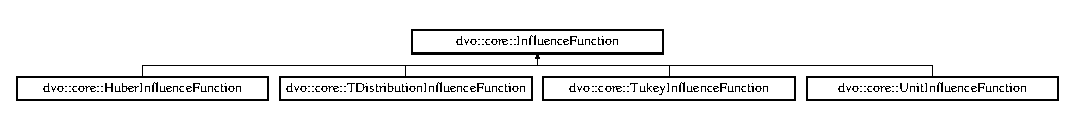
\includegraphics[height=1.120000cm]{classdvo_1_1core_1_1_influence_function}
\end{center}
\end{figure}
\subsection*{Public Member Functions}
\begin{DoxyCompactItemize}
\item 
virtual \mbox{\hyperlink{classdvo_1_1core_1_1_influence_function_afb3069251ce14c9213db1672c774e082}{$\sim$\+Influence\+Function}} ()
\item 
virtual float \mbox{\hyperlink{classdvo_1_1core_1_1_influence_function_a158082c763fa9de460e75a285bb91f1e}{value}} (const float \&x) const =0
\item 
virtual void \mbox{\hyperlink{classdvo_1_1core_1_1_influence_function_a4773b03ca609bc5d8391d09d92ab34ad}{configure}} (const float \&param)
\end{DoxyCompactItemize}


\subsection{Detailed Description}
Interface for influence functions. An influence function is the first derivative of a symmetric robust function p(sqrt(x)). The errors are assumed to be normalized to unit variance.

See\+: \char`\"{}\+Lucas-\/\+Kanade 20 Years On\+: A Unifying Framework\+: Part 2\char`\"{} 

\subsection{Constructor \& Destructor Documentation}
\mbox{\Hypertarget{classdvo_1_1core_1_1_influence_function_afb3069251ce14c9213db1672c774e082}\label{classdvo_1_1core_1_1_influence_function_afb3069251ce14c9213db1672c774e082}} 
\index{dvo\+::core\+::\+Influence\+Function@{dvo\+::core\+::\+Influence\+Function}!````~Influence\+Function@{$\sim$\+Influence\+Function}}
\index{````~Influence\+Function@{$\sim$\+Influence\+Function}!dvo\+::core\+::\+Influence\+Function@{dvo\+::core\+::\+Influence\+Function}}
\subsubsection{\texorpdfstring{$\sim$\+Influence\+Function()}{~InfluenceFunction()}}
{\footnotesize\ttfamily virtual dvo\+::core\+::\+Influence\+Function\+::$\sim$\+Influence\+Function (\begin{DoxyParamCaption}{ }\end{DoxyParamCaption})\hspace{0.3cm}{\ttfamily [inline]}, {\ttfamily [virtual]}}



\subsection{Member Function Documentation}
\mbox{\Hypertarget{classdvo_1_1core_1_1_influence_function_a4773b03ca609bc5d8391d09d92ab34ad}\label{classdvo_1_1core_1_1_influence_function_a4773b03ca609bc5d8391d09d92ab34ad}} 
\index{dvo\+::core\+::\+Influence\+Function@{dvo\+::core\+::\+Influence\+Function}!configure@{configure}}
\index{configure@{configure}!dvo\+::core\+::\+Influence\+Function@{dvo\+::core\+::\+Influence\+Function}}
\subsubsection{\texorpdfstring{configure()}{configure()}}
{\footnotesize\ttfamily virtual void dvo\+::core\+::\+Influence\+Function\+::configure (\begin{DoxyParamCaption}\item[{const float \&}]{param }\end{DoxyParamCaption})\hspace{0.3cm}{\ttfamily [inline]}, {\ttfamily [virtual]}}



Reimplemented in \mbox{\hyperlink{classdvo_1_1core_1_1_huber_influence_function_aab5a25ad6f632e829c8ad2ccf073fdec}{dvo\+::core\+::\+Huber\+Influence\+Function}}, \mbox{\hyperlink{classdvo_1_1core_1_1_t_distribution_influence_function_ad9030e81f013c14015c3ad97a2f821be}{dvo\+::core\+::\+T\+Distribution\+Influence\+Function}}, and \mbox{\hyperlink{classdvo_1_1core_1_1_tukey_influence_function_afa49d538d3eee4c545bb690a0aca0f11}{dvo\+::core\+::\+Tukey\+Influence\+Function}}.

\mbox{\Hypertarget{classdvo_1_1core_1_1_influence_function_a158082c763fa9de460e75a285bb91f1e}\label{classdvo_1_1core_1_1_influence_function_a158082c763fa9de460e75a285bb91f1e}} 
\index{dvo\+::core\+::\+Influence\+Function@{dvo\+::core\+::\+Influence\+Function}!value@{value}}
\index{value@{value}!dvo\+::core\+::\+Influence\+Function@{dvo\+::core\+::\+Influence\+Function}}
\subsubsection{\texorpdfstring{value()}{value()}}
{\footnotesize\ttfamily virtual float dvo\+::core\+::\+Influence\+Function\+::value (\begin{DoxyParamCaption}\item[{const float \&}]{x }\end{DoxyParamCaption}) const\hspace{0.3cm}{\ttfamily [pure virtual]}}



Implemented in \mbox{\hyperlink{classdvo_1_1core_1_1_huber_influence_function_af41e9e57eedcd25db690a1f41f3d6c8a}{dvo\+::core\+::\+Huber\+Influence\+Function}}, \mbox{\hyperlink{classdvo_1_1core_1_1_t_distribution_influence_function_a3210e7ab6f57975751e75845d3d22598}{dvo\+::core\+::\+T\+Distribution\+Influence\+Function}}, \mbox{\hyperlink{classdvo_1_1core_1_1_tukey_influence_function_a3a1829e6316ecffdceea8c54169c5ef1}{dvo\+::core\+::\+Tukey\+Influence\+Function}}, and \mbox{\hyperlink{classdvo_1_1core_1_1_unit_influence_function_a889eacebc6bcb0209a8ce37742dbbe71}{dvo\+::core\+::\+Unit\+Influence\+Function}}.



The documentation for this class was generated from the following file\+:\begin{DoxyCompactItemize}
\item 
dvo\+\_\+core/include/dvo/core/\mbox{\hyperlink{weight__calculation_8h}{weight\+\_\+calculation.\+h}}\end{DoxyCompactItemize}

\hypertarget{structdvo_1_1core_1_1_influence_functions}{}\section{dvo\+:\+:core\+:\+:Influence\+Functions Struct Reference}
\label{structdvo_1_1core_1_1_influence_functions}\index{dvo\+::core\+::\+Influence\+Functions@{dvo\+::core\+::\+Influence\+Functions}}


{\ttfamily \#include $<$weight\+\_\+calculation.\+h$>$}

\subsection*{Public Types}
\begin{DoxyCompactItemize}
\item 
enum \mbox{\hyperlink{structdvo_1_1core_1_1_influence_functions_a3fcb0831eb60e196888641a64fff665f}{enum\+\_\+t}} \{ \mbox{\hyperlink{structdvo_1_1core_1_1_influence_functions_a3fcb0831eb60e196888641a64fff665fad6ecc10a1c8928ad9a04636767dc31ff}{Unit}}, 
\mbox{\hyperlink{structdvo_1_1core_1_1_influence_functions_a3fcb0831eb60e196888641a64fff665fa4e74b42ef5f913e5bccd76f99cff1b35}{Tukey}}, 
\mbox{\hyperlink{structdvo_1_1core_1_1_influence_functions_a3fcb0831eb60e196888641a64fff665fa1d6bb04358a6bff2a7ae677ca16d74ad}{T\+Distribution}}, 
\mbox{\hyperlink{structdvo_1_1core_1_1_influence_functions_a3fcb0831eb60e196888641a64fff665fa2fe080ac9523516feeab8e7b3be9ad65}{Huber}}
 \}
\end{DoxyCompactItemize}
\subsection*{Static Public Member Functions}
\begin{DoxyCompactItemize}
\item 
static const char $\ast$ \mbox{\hyperlink{structdvo_1_1core_1_1_influence_functions_a8440157ce492ecc76e375d637a194db9}{str}} (\mbox{\hyperlink{structdvo_1_1core_1_1_influence_functions_a3fcb0831eb60e196888641a64fff665f}{enum\+\_\+t}} type)
\item 
static \mbox{\hyperlink{classdvo_1_1core_1_1_influence_function}{Influence\+Function}} $\ast$ \mbox{\hyperlink{structdvo_1_1core_1_1_influence_functions_a85f28604630e98484cc8534fea623c86}{get}} (\mbox{\hyperlink{structdvo_1_1core_1_1_influence_functions_a3fcb0831eb60e196888641a64fff665f}{enum\+\_\+t}} type)
\end{DoxyCompactItemize}


\subsection{Member Enumeration Documentation}
\mbox{\Hypertarget{structdvo_1_1core_1_1_influence_functions_a3fcb0831eb60e196888641a64fff665f}\label{structdvo_1_1core_1_1_influence_functions_a3fcb0831eb60e196888641a64fff665f}} 
\index{dvo\+::core\+::\+Influence\+Functions@{dvo\+::core\+::\+Influence\+Functions}!enum\+\_\+t@{enum\+\_\+t}}
\index{enum\+\_\+t@{enum\+\_\+t}!dvo\+::core\+::\+Influence\+Functions@{dvo\+::core\+::\+Influence\+Functions}}
\subsubsection{\texorpdfstring{enum\+\_\+t}{enum\_t}}
{\footnotesize\ttfamily enum \mbox{\hyperlink{structdvo_1_1core_1_1_influence_functions_a3fcb0831eb60e196888641a64fff665f}{dvo\+::core\+::\+Influence\+Functions\+::enum\+\_\+t}}}

\begin{DoxyEnumFields}{Enumerator}
\raisebox{\heightof{T}}[0pt][0pt]{\index{Unit@{Unit}!dvo\+::core\+::\+Influence\+Functions@{dvo\+::core\+::\+Influence\+Functions}}\index{dvo\+::core\+::\+Influence\+Functions@{dvo\+::core\+::\+Influence\+Functions}!Unit@{Unit}}}\mbox{\Hypertarget{structdvo_1_1core_1_1_influence_functions_a3fcb0831eb60e196888641a64fff665fad6ecc10a1c8928ad9a04636767dc31ff}\label{structdvo_1_1core_1_1_influence_functions_a3fcb0831eb60e196888641a64fff665fad6ecc10a1c8928ad9a04636767dc31ff}} 
Unit&\\
\hline

\raisebox{\heightof{T}}[0pt][0pt]{\index{Tukey@{Tukey}!dvo\+::core\+::\+Influence\+Functions@{dvo\+::core\+::\+Influence\+Functions}}\index{dvo\+::core\+::\+Influence\+Functions@{dvo\+::core\+::\+Influence\+Functions}!Tukey@{Tukey}}}\mbox{\Hypertarget{structdvo_1_1core_1_1_influence_functions_a3fcb0831eb60e196888641a64fff665fa4e74b42ef5f913e5bccd76f99cff1b35}\label{structdvo_1_1core_1_1_influence_functions_a3fcb0831eb60e196888641a64fff665fa4e74b42ef5f913e5bccd76f99cff1b35}} 
Tukey&\\
\hline

\raisebox{\heightof{T}}[0pt][0pt]{\index{T\+Distribution@{T\+Distribution}!dvo\+::core\+::\+Influence\+Functions@{dvo\+::core\+::\+Influence\+Functions}}\index{dvo\+::core\+::\+Influence\+Functions@{dvo\+::core\+::\+Influence\+Functions}!T\+Distribution@{T\+Distribution}}}\mbox{\Hypertarget{structdvo_1_1core_1_1_influence_functions_a3fcb0831eb60e196888641a64fff665fa1d6bb04358a6bff2a7ae677ca16d74ad}\label{structdvo_1_1core_1_1_influence_functions_a3fcb0831eb60e196888641a64fff665fa1d6bb04358a6bff2a7ae677ca16d74ad}} 
T\+Distribution&\\
\hline

\raisebox{\heightof{T}}[0pt][0pt]{\index{Huber@{Huber}!dvo\+::core\+::\+Influence\+Functions@{dvo\+::core\+::\+Influence\+Functions}}\index{dvo\+::core\+::\+Influence\+Functions@{dvo\+::core\+::\+Influence\+Functions}!Huber@{Huber}}}\mbox{\Hypertarget{structdvo_1_1core_1_1_influence_functions_a3fcb0831eb60e196888641a64fff665fa2fe080ac9523516feeab8e7b3be9ad65}\label{structdvo_1_1core_1_1_influence_functions_a3fcb0831eb60e196888641a64fff665fa2fe080ac9523516feeab8e7b3be9ad65}} 
Huber&\\
\hline

\end{DoxyEnumFields}


\subsection{Member Function Documentation}
\mbox{\Hypertarget{structdvo_1_1core_1_1_influence_functions_a85f28604630e98484cc8534fea623c86}\label{structdvo_1_1core_1_1_influence_functions_a85f28604630e98484cc8534fea623c86}} 
\index{dvo\+::core\+::\+Influence\+Functions@{dvo\+::core\+::\+Influence\+Functions}!get@{get}}
\index{get@{get}!dvo\+::core\+::\+Influence\+Functions@{dvo\+::core\+::\+Influence\+Functions}}
\subsubsection{\texorpdfstring{get()}{get()}}
{\footnotesize\ttfamily \mbox{\hyperlink{classdvo_1_1core_1_1_influence_function}{Influence\+Function}} $\ast$ dvo\+::core\+::\+Influence\+Functions\+::get (\begin{DoxyParamCaption}\item[{\mbox{\hyperlink{structdvo_1_1core_1_1_influence_functions_a3fcb0831eb60e196888641a64fff665f}{Influence\+Functions\+::enum\+\_\+t}}}]{type }\end{DoxyParamCaption})\hspace{0.3cm}{\ttfamily [static]}}

\mbox{\Hypertarget{structdvo_1_1core_1_1_influence_functions_a8440157ce492ecc76e375d637a194db9}\label{structdvo_1_1core_1_1_influence_functions_a8440157ce492ecc76e375d637a194db9}} 
\index{dvo\+::core\+::\+Influence\+Functions@{dvo\+::core\+::\+Influence\+Functions}!str@{str}}
\index{str@{str}!dvo\+::core\+::\+Influence\+Functions@{dvo\+::core\+::\+Influence\+Functions}}
\subsubsection{\texorpdfstring{str()}{str()}}
{\footnotesize\ttfamily const char $\ast$ dvo\+::core\+::\+Influence\+Functions\+::str (\begin{DoxyParamCaption}\item[{\mbox{\hyperlink{structdvo_1_1core_1_1_influence_functions_a3fcb0831eb60e196888641a64fff665f}{enum\+\_\+t}}}]{type }\end{DoxyParamCaption})\hspace{0.3cm}{\ttfamily [static]}}



The documentation for this struct was generated from the following files\+:\begin{DoxyCompactItemize}
\item 
dvo\+\_\+core/include/dvo/core/\mbox{\hyperlink{weight__calculation_8h}{weight\+\_\+calculation.\+h}}\item 
dvo\+\_\+core/src/core/\mbox{\hyperlink{weight__calculation_8cpp}{weight\+\_\+calculation.\+cpp}}\end{DoxyCompactItemize}

\hypertarget{structdvo_1_1core_1_1_interpolation}{}\section{dvo\+:\+:core\+:\+:Interpolation Struct Reference}
\label{structdvo_1_1core_1_1_interpolation}\index{dvo\+::core\+::\+Interpolation@{dvo\+::core\+::\+Interpolation}}


{\ttfamily \#include $<$interpolation.\+h$>$}

\subsection*{Static Public Member Functions}
\begin{DoxyCompactItemize}
\item 
static \mbox{\hyperlink{namespacedvo_1_1core_a59740d7c1f271a6ec8cb2b5c42e7a3f2}{Intensity\+Type}} \mbox{\hyperlink{structdvo_1_1core_1_1_interpolation_a5ea50138a3a09dbbbc056e2b67526dfd}{none}} (const cv\+::\+Mat \&img, float x, float y)
\item 
static \mbox{\hyperlink{namespacedvo_1_1core_a59740d7c1f271a6ec8cb2b5c42e7a3f2}{Intensity\+Type}} \mbox{\hyperlink{structdvo_1_1core_1_1_interpolation_afa685d096b310ee18ec6e5491d2a80d6}{bilinear}} (const cv\+::\+Mat \&img, float x, float y)
\item 
static \mbox{\hyperlink{namespacedvo_1_1core_a59740d7c1f271a6ec8cb2b5c42e7a3f2}{Intensity\+Type}} \mbox{\hyperlink{structdvo_1_1core_1_1_interpolation_a25af1de0ec0b6547e9f06b70abb18e0b}{bilinear\+With\+Depth\+Buffer}} (const cv\+::\+Mat \&intensity, const cv\+::\+Mat \&depth, const float \&x, const float \&y, const float \&z)
\end{DoxyCompactItemize}


\subsection{Member Function Documentation}
\mbox{\Hypertarget{structdvo_1_1core_1_1_interpolation_afa685d096b310ee18ec6e5491d2a80d6}\label{structdvo_1_1core_1_1_interpolation_afa685d096b310ee18ec6e5491d2a80d6}} 
\index{dvo\+::core\+::\+Interpolation@{dvo\+::core\+::\+Interpolation}!bilinear@{bilinear}}
\index{bilinear@{bilinear}!dvo\+::core\+::\+Interpolation@{dvo\+::core\+::\+Interpolation}}
\subsubsection{\texorpdfstring{bilinear()}{bilinear()}}
{\footnotesize\ttfamily \mbox{\hyperlink{namespacedvo_1_1core_a59740d7c1f271a6ec8cb2b5c42e7a3f2}{Intensity\+Type}} dvo\+::core\+::\+Interpolation\+::bilinear (\begin{DoxyParamCaption}\item[{const cv\+::\+Mat \&}]{img,  }\item[{float}]{x,  }\item[{float}]{y }\end{DoxyParamCaption})\hspace{0.3cm}{\ttfamily [static]}}

\mbox{\Hypertarget{structdvo_1_1core_1_1_interpolation_a25af1de0ec0b6547e9f06b70abb18e0b}\label{structdvo_1_1core_1_1_interpolation_a25af1de0ec0b6547e9f06b70abb18e0b}} 
\index{dvo\+::core\+::\+Interpolation@{dvo\+::core\+::\+Interpolation}!bilinear\+With\+Depth\+Buffer@{bilinear\+With\+Depth\+Buffer}}
\index{bilinear\+With\+Depth\+Buffer@{bilinear\+With\+Depth\+Buffer}!dvo\+::core\+::\+Interpolation@{dvo\+::core\+::\+Interpolation}}
\subsubsection{\texorpdfstring{bilinear\+With\+Depth\+Buffer()}{bilinearWithDepthBuffer()}}
{\footnotesize\ttfamily \mbox{\hyperlink{namespacedvo_1_1core_a59740d7c1f271a6ec8cb2b5c42e7a3f2}{Intensity\+Type}} dvo\+::core\+::\+Interpolation\+::bilinear\+With\+Depth\+Buffer (\begin{DoxyParamCaption}\item[{const cv\+::\+Mat \&}]{intensity,  }\item[{const cv\+::\+Mat \&}]{depth,  }\item[{const float \&}]{x,  }\item[{const float \&}]{y,  }\item[{const float \&}]{z }\end{DoxyParamCaption})\hspace{0.3cm}{\ttfamily [static]}}

\mbox{\Hypertarget{structdvo_1_1core_1_1_interpolation_a5ea50138a3a09dbbbc056e2b67526dfd}\label{structdvo_1_1core_1_1_interpolation_a5ea50138a3a09dbbbc056e2b67526dfd}} 
\index{dvo\+::core\+::\+Interpolation@{dvo\+::core\+::\+Interpolation}!none@{none}}
\index{none@{none}!dvo\+::core\+::\+Interpolation@{dvo\+::core\+::\+Interpolation}}
\subsubsection{\texorpdfstring{none()}{none()}}
{\footnotesize\ttfamily \mbox{\hyperlink{namespacedvo_1_1core_a59740d7c1f271a6ec8cb2b5c42e7a3f2}{Intensity\+Type}} dvo\+::core\+::\+Interpolation\+::none (\begin{DoxyParamCaption}\item[{const cv\+::\+Mat \&}]{img,  }\item[{float}]{x,  }\item[{float}]{y }\end{DoxyParamCaption})\hspace{0.3cm}{\ttfamily [static]}}



The documentation for this struct was generated from the following files\+:\begin{DoxyCompactItemize}
\item 
dvo\+\_\+core/include/dvo/core/\mbox{\hyperlink{interpolation_8h}{interpolation.\+h}}\item 
dvo\+\_\+core/src/core/\mbox{\hyperlink{interpolation_8cpp}{interpolation.\+cpp}}\end{DoxyCompactItemize}

\hypertarget{structdvo_1_1core_1_1_intrinsic_matrix}{}\section{dvo\+:\+:core\+:\+:Intrinsic\+Matrix Struct Reference}
\label{structdvo_1_1core_1_1_intrinsic_matrix}\index{dvo\+::core\+::\+Intrinsic\+Matrix@{dvo\+::core\+::\+Intrinsic\+Matrix}}


{\ttfamily \#include $<$intrinsic\+\_\+matrix.\+h$>$}

\subsection*{Classes}
\begin{DoxyCompactItemize}
\item 
struct \mbox{\hyperlink{structdvo_1_1core_1_1_intrinsic_matrix_1_1_equal}{Equal}}
\item 
struct \mbox{\hyperlink{structdvo_1_1core_1_1_intrinsic_matrix_1_1_hash}{Hash}}
\end{DoxyCompactItemize}
\subsection*{Public Member Functions}
\begin{DoxyCompactItemize}
\item 
E\+I\+G\+E\+N\+\_\+\+M\+A\+K\+E\+\_\+\+A\+L\+I\+G\+N\+E\+D\+\_\+\+O\+P\+E\+R\+A\+T\+O\+R\+\_\+\+N\+EW \mbox{\hyperlink{structdvo_1_1core_1_1_intrinsic_matrix_a2b25541b5d84522454f177f446c5ee2a}{Intrinsic\+Matrix}} ()
\item 
\mbox{\hyperlink{structdvo_1_1core_1_1_intrinsic_matrix_ac7b94dc0f3db8dd63aff0dd6c1315ab4}{Intrinsic\+Matrix}} (const \mbox{\hyperlink{structdvo_1_1core_1_1_intrinsic_matrix}{Intrinsic\+Matrix}} \&other)
\item 
float \mbox{\hyperlink{structdvo_1_1core_1_1_intrinsic_matrix_aa9431c46e33728102f94eed724281aea}{fx}} () const
\item 
float \mbox{\hyperlink{structdvo_1_1core_1_1_intrinsic_matrix_a4d96c81bec804d54ec778a66c822566d}{fy}} () const
\item 
float \mbox{\hyperlink{structdvo_1_1core_1_1_intrinsic_matrix_ae882a75257467c10b0ca5344410b6a3f}{ox}} () const
\item 
float \mbox{\hyperlink{structdvo_1_1core_1_1_intrinsic_matrix_ad0d6657452709e25bbcc7bd7b54b5d5b}{oy}} () const
\item 
void \mbox{\hyperlink{structdvo_1_1core_1_1_intrinsic_matrix_a796dd58464c65afafd8b45d4366b71b4}{invert\+Offset}} ()
\item 
void \mbox{\hyperlink{structdvo_1_1core_1_1_intrinsic_matrix_a425932a5bc42fcde9dc768aecd60f7ef}{scale}} (float factor)
\end{DoxyCompactItemize}
\subsection*{Static Public Member Functions}
\begin{DoxyCompactItemize}
\item 
static \mbox{\hyperlink{structdvo_1_1core_1_1_intrinsic_matrix}{Intrinsic\+Matrix}} \mbox{\hyperlink{structdvo_1_1core_1_1_intrinsic_matrix_afe57d9817ec2a275482338744a80ac08}{create}} (float \mbox{\hyperlink{structdvo_1_1core_1_1_intrinsic_matrix_aa9431c46e33728102f94eed724281aea}{fx}}, float \mbox{\hyperlink{structdvo_1_1core_1_1_intrinsic_matrix_a4d96c81bec804d54ec778a66c822566d}{fy}}, float \mbox{\hyperlink{structdvo_1_1core_1_1_intrinsic_matrix_ae882a75257467c10b0ca5344410b6a3f}{ox}}, float \mbox{\hyperlink{structdvo_1_1core_1_1_intrinsic_matrix_ad0d6657452709e25bbcc7bd7b54b5d5b}{oy}})
\end{DoxyCompactItemize}
\subsection*{Public Attributes}
\begin{DoxyCompactItemize}
\item 
Eigen\+::\+Matrix3f \mbox{\hyperlink{structdvo_1_1core_1_1_intrinsic_matrix_ab76264a79c0fce5dbeb590cdbd3d6c46}{data}}
\end{DoxyCompactItemize}


\subsection{Constructor \& Destructor Documentation}
\mbox{\Hypertarget{structdvo_1_1core_1_1_intrinsic_matrix_a2b25541b5d84522454f177f446c5ee2a}\label{structdvo_1_1core_1_1_intrinsic_matrix_a2b25541b5d84522454f177f446c5ee2a}} 
\index{dvo\+::core\+::\+Intrinsic\+Matrix@{dvo\+::core\+::\+Intrinsic\+Matrix}!Intrinsic\+Matrix@{Intrinsic\+Matrix}}
\index{Intrinsic\+Matrix@{Intrinsic\+Matrix}!dvo\+::core\+::\+Intrinsic\+Matrix@{dvo\+::core\+::\+Intrinsic\+Matrix}}
\subsubsection{\texorpdfstring{Intrinsic\+Matrix()}{IntrinsicMatrix()}\hspace{0.1cm}{\footnotesize\ttfamily [1/2]}}
{\footnotesize\ttfamily E\+I\+G\+E\+N\+\_\+\+M\+A\+K\+E\+\_\+\+A\+L\+I\+G\+N\+E\+D\+\_\+\+O\+P\+E\+R\+A\+T\+O\+R\+\_\+\+N\+EW dvo\+::core\+::\+Intrinsic\+Matrix\+::\+Intrinsic\+Matrix (\begin{DoxyParamCaption}{ }\end{DoxyParamCaption})\hspace{0.3cm}{\ttfamily [inline]}}

\mbox{\Hypertarget{structdvo_1_1core_1_1_intrinsic_matrix_ac7b94dc0f3db8dd63aff0dd6c1315ab4}\label{structdvo_1_1core_1_1_intrinsic_matrix_ac7b94dc0f3db8dd63aff0dd6c1315ab4}} 
\index{dvo\+::core\+::\+Intrinsic\+Matrix@{dvo\+::core\+::\+Intrinsic\+Matrix}!Intrinsic\+Matrix@{Intrinsic\+Matrix}}
\index{Intrinsic\+Matrix@{Intrinsic\+Matrix}!dvo\+::core\+::\+Intrinsic\+Matrix@{dvo\+::core\+::\+Intrinsic\+Matrix}}
\subsubsection{\texorpdfstring{Intrinsic\+Matrix()}{IntrinsicMatrix()}\hspace{0.1cm}{\footnotesize\ttfamily [2/2]}}
{\footnotesize\ttfamily dvo\+::core\+::\+Intrinsic\+Matrix\+::\+Intrinsic\+Matrix (\begin{DoxyParamCaption}\item[{const \mbox{\hyperlink{structdvo_1_1core_1_1_intrinsic_matrix}{Intrinsic\+Matrix}} \&}]{other }\end{DoxyParamCaption})}



\subsection{Member Function Documentation}
\mbox{\Hypertarget{structdvo_1_1core_1_1_intrinsic_matrix_afe57d9817ec2a275482338744a80ac08}\label{structdvo_1_1core_1_1_intrinsic_matrix_afe57d9817ec2a275482338744a80ac08}} 
\index{dvo\+::core\+::\+Intrinsic\+Matrix@{dvo\+::core\+::\+Intrinsic\+Matrix}!create@{create}}
\index{create@{create}!dvo\+::core\+::\+Intrinsic\+Matrix@{dvo\+::core\+::\+Intrinsic\+Matrix}}
\subsubsection{\texorpdfstring{create()}{create()}}
{\footnotesize\ttfamily \mbox{\hyperlink{structdvo_1_1core_1_1_intrinsic_matrix}{Intrinsic\+Matrix}} dvo\+::core\+::\+Intrinsic\+Matrix\+::create (\begin{DoxyParamCaption}\item[{float}]{fx,  }\item[{float}]{fy,  }\item[{float}]{ox,  }\item[{float}]{oy }\end{DoxyParamCaption})\hspace{0.3cm}{\ttfamily [static]}}

\mbox{\Hypertarget{structdvo_1_1core_1_1_intrinsic_matrix_aa9431c46e33728102f94eed724281aea}\label{structdvo_1_1core_1_1_intrinsic_matrix_aa9431c46e33728102f94eed724281aea}} 
\index{dvo\+::core\+::\+Intrinsic\+Matrix@{dvo\+::core\+::\+Intrinsic\+Matrix}!fx@{fx}}
\index{fx@{fx}!dvo\+::core\+::\+Intrinsic\+Matrix@{dvo\+::core\+::\+Intrinsic\+Matrix}}
\subsubsection{\texorpdfstring{fx()}{fx()}}
{\footnotesize\ttfamily float dvo\+::core\+::\+Intrinsic\+Matrix\+::fx (\begin{DoxyParamCaption}{ }\end{DoxyParamCaption}) const}

\mbox{\Hypertarget{structdvo_1_1core_1_1_intrinsic_matrix_a4d96c81bec804d54ec778a66c822566d}\label{structdvo_1_1core_1_1_intrinsic_matrix_a4d96c81bec804d54ec778a66c822566d}} 
\index{dvo\+::core\+::\+Intrinsic\+Matrix@{dvo\+::core\+::\+Intrinsic\+Matrix}!fy@{fy}}
\index{fy@{fy}!dvo\+::core\+::\+Intrinsic\+Matrix@{dvo\+::core\+::\+Intrinsic\+Matrix}}
\subsubsection{\texorpdfstring{fy()}{fy()}}
{\footnotesize\ttfamily float dvo\+::core\+::\+Intrinsic\+Matrix\+::fy (\begin{DoxyParamCaption}{ }\end{DoxyParamCaption}) const}

\mbox{\Hypertarget{structdvo_1_1core_1_1_intrinsic_matrix_a796dd58464c65afafd8b45d4366b71b4}\label{structdvo_1_1core_1_1_intrinsic_matrix_a796dd58464c65afafd8b45d4366b71b4}} 
\index{dvo\+::core\+::\+Intrinsic\+Matrix@{dvo\+::core\+::\+Intrinsic\+Matrix}!invert\+Offset@{invert\+Offset}}
\index{invert\+Offset@{invert\+Offset}!dvo\+::core\+::\+Intrinsic\+Matrix@{dvo\+::core\+::\+Intrinsic\+Matrix}}
\subsubsection{\texorpdfstring{invert\+Offset()}{invertOffset()}}
{\footnotesize\ttfamily void dvo\+::core\+::\+Intrinsic\+Matrix\+::invert\+Offset (\begin{DoxyParamCaption}{ }\end{DoxyParamCaption})}

\mbox{\Hypertarget{structdvo_1_1core_1_1_intrinsic_matrix_ae882a75257467c10b0ca5344410b6a3f}\label{structdvo_1_1core_1_1_intrinsic_matrix_ae882a75257467c10b0ca5344410b6a3f}} 
\index{dvo\+::core\+::\+Intrinsic\+Matrix@{dvo\+::core\+::\+Intrinsic\+Matrix}!ox@{ox}}
\index{ox@{ox}!dvo\+::core\+::\+Intrinsic\+Matrix@{dvo\+::core\+::\+Intrinsic\+Matrix}}
\subsubsection{\texorpdfstring{ox()}{ox()}}
{\footnotesize\ttfamily float dvo\+::core\+::\+Intrinsic\+Matrix\+::ox (\begin{DoxyParamCaption}{ }\end{DoxyParamCaption}) const}

\mbox{\Hypertarget{structdvo_1_1core_1_1_intrinsic_matrix_ad0d6657452709e25bbcc7bd7b54b5d5b}\label{structdvo_1_1core_1_1_intrinsic_matrix_ad0d6657452709e25bbcc7bd7b54b5d5b}} 
\index{dvo\+::core\+::\+Intrinsic\+Matrix@{dvo\+::core\+::\+Intrinsic\+Matrix}!oy@{oy}}
\index{oy@{oy}!dvo\+::core\+::\+Intrinsic\+Matrix@{dvo\+::core\+::\+Intrinsic\+Matrix}}
\subsubsection{\texorpdfstring{oy()}{oy()}}
{\footnotesize\ttfamily float dvo\+::core\+::\+Intrinsic\+Matrix\+::oy (\begin{DoxyParamCaption}{ }\end{DoxyParamCaption}) const}

\mbox{\Hypertarget{structdvo_1_1core_1_1_intrinsic_matrix_a425932a5bc42fcde9dc768aecd60f7ef}\label{structdvo_1_1core_1_1_intrinsic_matrix_a425932a5bc42fcde9dc768aecd60f7ef}} 
\index{dvo\+::core\+::\+Intrinsic\+Matrix@{dvo\+::core\+::\+Intrinsic\+Matrix}!scale@{scale}}
\index{scale@{scale}!dvo\+::core\+::\+Intrinsic\+Matrix@{dvo\+::core\+::\+Intrinsic\+Matrix}}
\subsubsection{\texorpdfstring{scale()}{scale()}}
{\footnotesize\ttfamily void dvo\+::core\+::\+Intrinsic\+Matrix\+::scale (\begin{DoxyParamCaption}\item[{float}]{factor }\end{DoxyParamCaption})}



\subsection{Member Data Documentation}
\mbox{\Hypertarget{structdvo_1_1core_1_1_intrinsic_matrix_ab76264a79c0fce5dbeb590cdbd3d6c46}\label{structdvo_1_1core_1_1_intrinsic_matrix_ab76264a79c0fce5dbeb590cdbd3d6c46}} 
\index{dvo\+::core\+::\+Intrinsic\+Matrix@{dvo\+::core\+::\+Intrinsic\+Matrix}!data@{data}}
\index{data@{data}!dvo\+::core\+::\+Intrinsic\+Matrix@{dvo\+::core\+::\+Intrinsic\+Matrix}}
\subsubsection{\texorpdfstring{data}{data}}
{\footnotesize\ttfamily Eigen\+::\+Matrix3f dvo\+::core\+::\+Intrinsic\+Matrix\+::data}



The documentation for this struct was generated from the following files\+:\begin{DoxyCompactItemize}
\item 
dvo\+\_\+core/include/dvo/core/\mbox{\hyperlink{intrinsic__matrix_8h}{intrinsic\+\_\+matrix.\+h}}\item 
dvo\+\_\+core/src/core/\mbox{\hyperlink{intrinsic__matrix_8cpp}{intrinsic\+\_\+matrix.\+cpp}}\end{DoxyCompactItemize}

\hypertarget{structdvo_1_1_dense_tracker_1_1_iteration_context}{}\section{dvo\+:\+:Dense\+Tracker\+:\+:Iteration\+Context Struct Reference}
\label{structdvo_1_1_dense_tracker_1_1_iteration_context}\index{dvo\+::\+Dense\+Tracker\+::\+Iteration\+Context@{dvo\+::\+Dense\+Tracker\+::\+Iteration\+Context}}


{\ttfamily \#include $<$dense\+\_\+tracking.\+h$>$}

\subsection*{Public Member Functions}
\begin{DoxyCompactItemize}
\item 
\mbox{\hyperlink{structdvo_1_1_dense_tracker_1_1_iteration_context_ab2e12923bbbc9b540cf8139d3a4d3f33}{Iteration\+Context}} (const \mbox{\hyperlink{structdvo_1_1_dense_tracker_1_1_config}{Config}} \&\mbox{\hyperlink{structdvo_1_1_dense_tracker_1_1_iteration_context_a56d4fa3811b2b6d24243d2d0ea0d7348}{cfg}})
\item 
bool \mbox{\hyperlink{structdvo_1_1_dense_tracker_1_1_iteration_context_a67e450af240d213a8021d57bc11ac42a}{Is\+First\+Iteration}} () const
\item 
bool \mbox{\hyperlink{structdvo_1_1_dense_tracker_1_1_iteration_context_a419d0a3e80b785735eac4934fddf827f}{Is\+First\+Iteration\+On\+Level}} () const
\item 
bool \mbox{\hyperlink{structdvo_1_1_dense_tracker_1_1_iteration_context_a69730e1cd4e3c4bc183a181fe9026f40}{Is\+First\+Level}} () const
\item 
bool \mbox{\hyperlink{structdvo_1_1_dense_tracker_1_1_iteration_context_ac27dac99b037feb1e2bbce3b3315dd4a}{Is\+Last\+Level}} () const
\item 
bool \mbox{\hyperlink{structdvo_1_1_dense_tracker_1_1_iteration_context_aa15a70a3a1af2f73c07f7bc7eb933a9b}{Iterations\+Exceeded}} () const
\item 
double \mbox{\hyperlink{structdvo_1_1_dense_tracker_1_1_iteration_context_acc9cb928fcc0017d050d25393b4ed379}{Error\+Diff}} () const
\end{DoxyCompactItemize}
\subsection*{Public Attributes}
\begin{DoxyCompactItemize}
\item 
const \mbox{\hyperlink{structdvo_1_1_dense_tracker_1_1_config}{Config}} \& \mbox{\hyperlink{structdvo_1_1_dense_tracker_1_1_iteration_context_a56d4fa3811b2b6d24243d2d0ea0d7348}{cfg}}
\item 
int \mbox{\hyperlink{structdvo_1_1_dense_tracker_1_1_iteration_context_a7efda75ce2066b72f0d7e94badb2d560}{Level}}
\item 
int \mbox{\hyperlink{structdvo_1_1_dense_tracker_1_1_iteration_context_afc12b998ec8732853a00ab396e20986d}{Iteration}}
\item 
size\+\_\+t \mbox{\hyperlink{structdvo_1_1_dense_tracker_1_1_iteration_context_a69908efda33537ec90b69af2bcf4d3a1}{Num\+Constraints}}
\item 
double \mbox{\hyperlink{structdvo_1_1_dense_tracker_1_1_iteration_context_acaa2799f500e5b1029ecd13d6a384baf}{Error}}
\item 
double \mbox{\hyperlink{structdvo_1_1_dense_tracker_1_1_iteration_context_aed3ead8aa09b40e80a7e58249ff3a54d}{Last\+Error}}
\end{DoxyCompactItemize}


\subsection{Constructor \& Destructor Documentation}
\mbox{\Hypertarget{structdvo_1_1_dense_tracker_1_1_iteration_context_ab2e12923bbbc9b540cf8139d3a4d3f33}\label{structdvo_1_1_dense_tracker_1_1_iteration_context_ab2e12923bbbc9b540cf8139d3a4d3f33}} 
\index{dvo\+::\+Dense\+Tracker\+::\+Iteration\+Context@{dvo\+::\+Dense\+Tracker\+::\+Iteration\+Context}!Iteration\+Context@{Iteration\+Context}}
\index{Iteration\+Context@{Iteration\+Context}!dvo\+::\+Dense\+Tracker\+::\+Iteration\+Context@{dvo\+::\+Dense\+Tracker\+::\+Iteration\+Context}}
\subsubsection{\texorpdfstring{Iteration\+Context()}{IterationContext()}}
{\footnotesize\ttfamily dvo\+::\+Dense\+Tracker\+::\+Iteration\+Context\+::\+Iteration\+Context (\begin{DoxyParamCaption}\item[{const \mbox{\hyperlink{structdvo_1_1_dense_tracker_1_1_config}{Config}} \&}]{cfg }\end{DoxyParamCaption})}



\subsection{Member Function Documentation}
\mbox{\Hypertarget{structdvo_1_1_dense_tracker_1_1_iteration_context_acc9cb928fcc0017d050d25393b4ed379}\label{structdvo_1_1_dense_tracker_1_1_iteration_context_acc9cb928fcc0017d050d25393b4ed379}} 
\index{dvo\+::\+Dense\+Tracker\+::\+Iteration\+Context@{dvo\+::\+Dense\+Tracker\+::\+Iteration\+Context}!Error\+Diff@{Error\+Diff}}
\index{Error\+Diff@{Error\+Diff}!dvo\+::\+Dense\+Tracker\+::\+Iteration\+Context@{dvo\+::\+Dense\+Tracker\+::\+Iteration\+Context}}
\subsubsection{\texorpdfstring{Error\+Diff()}{ErrorDiff()}}
{\footnotesize\ttfamily double dvo\+::\+Dense\+Tracker\+::\+Iteration\+Context\+::\+Error\+Diff (\begin{DoxyParamCaption}{ }\end{DoxyParamCaption}) const}

\mbox{\Hypertarget{structdvo_1_1_dense_tracker_1_1_iteration_context_a67e450af240d213a8021d57bc11ac42a}\label{structdvo_1_1_dense_tracker_1_1_iteration_context_a67e450af240d213a8021d57bc11ac42a}} 
\index{dvo\+::\+Dense\+Tracker\+::\+Iteration\+Context@{dvo\+::\+Dense\+Tracker\+::\+Iteration\+Context}!Is\+First\+Iteration@{Is\+First\+Iteration}}
\index{Is\+First\+Iteration@{Is\+First\+Iteration}!dvo\+::\+Dense\+Tracker\+::\+Iteration\+Context@{dvo\+::\+Dense\+Tracker\+::\+Iteration\+Context}}
\subsubsection{\texorpdfstring{Is\+First\+Iteration()}{IsFirstIteration()}}
{\footnotesize\ttfamily bool dvo\+::\+Dense\+Tracker\+::\+Iteration\+Context\+::\+Is\+First\+Iteration (\begin{DoxyParamCaption}{ }\end{DoxyParamCaption}) const}

\mbox{\Hypertarget{structdvo_1_1_dense_tracker_1_1_iteration_context_a419d0a3e80b785735eac4934fddf827f}\label{structdvo_1_1_dense_tracker_1_1_iteration_context_a419d0a3e80b785735eac4934fddf827f}} 
\index{dvo\+::\+Dense\+Tracker\+::\+Iteration\+Context@{dvo\+::\+Dense\+Tracker\+::\+Iteration\+Context}!Is\+First\+Iteration\+On\+Level@{Is\+First\+Iteration\+On\+Level}}
\index{Is\+First\+Iteration\+On\+Level@{Is\+First\+Iteration\+On\+Level}!dvo\+::\+Dense\+Tracker\+::\+Iteration\+Context@{dvo\+::\+Dense\+Tracker\+::\+Iteration\+Context}}
\subsubsection{\texorpdfstring{Is\+First\+Iteration\+On\+Level()}{IsFirstIterationOnLevel()}}
{\footnotesize\ttfamily bool dvo\+::\+Dense\+Tracker\+::\+Iteration\+Context\+::\+Is\+First\+Iteration\+On\+Level (\begin{DoxyParamCaption}{ }\end{DoxyParamCaption}) const}

\mbox{\Hypertarget{structdvo_1_1_dense_tracker_1_1_iteration_context_a69730e1cd4e3c4bc183a181fe9026f40}\label{structdvo_1_1_dense_tracker_1_1_iteration_context_a69730e1cd4e3c4bc183a181fe9026f40}} 
\index{dvo\+::\+Dense\+Tracker\+::\+Iteration\+Context@{dvo\+::\+Dense\+Tracker\+::\+Iteration\+Context}!Is\+First\+Level@{Is\+First\+Level}}
\index{Is\+First\+Level@{Is\+First\+Level}!dvo\+::\+Dense\+Tracker\+::\+Iteration\+Context@{dvo\+::\+Dense\+Tracker\+::\+Iteration\+Context}}
\subsubsection{\texorpdfstring{Is\+First\+Level()}{IsFirstLevel()}}
{\footnotesize\ttfamily bool dvo\+::\+Dense\+Tracker\+::\+Iteration\+Context\+::\+Is\+First\+Level (\begin{DoxyParamCaption}{ }\end{DoxyParamCaption}) const}

\mbox{\Hypertarget{structdvo_1_1_dense_tracker_1_1_iteration_context_ac27dac99b037feb1e2bbce3b3315dd4a}\label{structdvo_1_1_dense_tracker_1_1_iteration_context_ac27dac99b037feb1e2bbce3b3315dd4a}} 
\index{dvo\+::\+Dense\+Tracker\+::\+Iteration\+Context@{dvo\+::\+Dense\+Tracker\+::\+Iteration\+Context}!Is\+Last\+Level@{Is\+Last\+Level}}
\index{Is\+Last\+Level@{Is\+Last\+Level}!dvo\+::\+Dense\+Tracker\+::\+Iteration\+Context@{dvo\+::\+Dense\+Tracker\+::\+Iteration\+Context}}
\subsubsection{\texorpdfstring{Is\+Last\+Level()}{IsLastLevel()}}
{\footnotesize\ttfamily bool dvo\+::\+Dense\+Tracker\+::\+Iteration\+Context\+::\+Is\+Last\+Level (\begin{DoxyParamCaption}{ }\end{DoxyParamCaption}) const}

\mbox{\Hypertarget{structdvo_1_1_dense_tracker_1_1_iteration_context_aa15a70a3a1af2f73c07f7bc7eb933a9b}\label{structdvo_1_1_dense_tracker_1_1_iteration_context_aa15a70a3a1af2f73c07f7bc7eb933a9b}} 
\index{dvo\+::\+Dense\+Tracker\+::\+Iteration\+Context@{dvo\+::\+Dense\+Tracker\+::\+Iteration\+Context}!Iterations\+Exceeded@{Iterations\+Exceeded}}
\index{Iterations\+Exceeded@{Iterations\+Exceeded}!dvo\+::\+Dense\+Tracker\+::\+Iteration\+Context@{dvo\+::\+Dense\+Tracker\+::\+Iteration\+Context}}
\subsubsection{\texorpdfstring{Iterations\+Exceeded()}{IterationsExceeded()}}
{\footnotesize\ttfamily bool dvo\+::\+Dense\+Tracker\+::\+Iteration\+Context\+::\+Iterations\+Exceeded (\begin{DoxyParamCaption}{ }\end{DoxyParamCaption}) const}



\subsection{Member Data Documentation}
\mbox{\Hypertarget{structdvo_1_1_dense_tracker_1_1_iteration_context_a56d4fa3811b2b6d24243d2d0ea0d7348}\label{structdvo_1_1_dense_tracker_1_1_iteration_context_a56d4fa3811b2b6d24243d2d0ea0d7348}} 
\index{dvo\+::\+Dense\+Tracker\+::\+Iteration\+Context@{dvo\+::\+Dense\+Tracker\+::\+Iteration\+Context}!cfg@{cfg}}
\index{cfg@{cfg}!dvo\+::\+Dense\+Tracker\+::\+Iteration\+Context@{dvo\+::\+Dense\+Tracker\+::\+Iteration\+Context}}
\subsubsection{\texorpdfstring{cfg}{cfg}}
{\footnotesize\ttfamily const \mbox{\hyperlink{structdvo_1_1_dense_tracker_1_1_config}{Config}}\& dvo\+::\+Dense\+Tracker\+::\+Iteration\+Context\+::cfg}

\mbox{\Hypertarget{structdvo_1_1_dense_tracker_1_1_iteration_context_acaa2799f500e5b1029ecd13d6a384baf}\label{structdvo_1_1_dense_tracker_1_1_iteration_context_acaa2799f500e5b1029ecd13d6a384baf}} 
\index{dvo\+::\+Dense\+Tracker\+::\+Iteration\+Context@{dvo\+::\+Dense\+Tracker\+::\+Iteration\+Context}!Error@{Error}}
\index{Error@{Error}!dvo\+::\+Dense\+Tracker\+::\+Iteration\+Context@{dvo\+::\+Dense\+Tracker\+::\+Iteration\+Context}}
\subsubsection{\texorpdfstring{Error}{Error}}
{\footnotesize\ttfamily double dvo\+::\+Dense\+Tracker\+::\+Iteration\+Context\+::\+Error}

\mbox{\Hypertarget{structdvo_1_1_dense_tracker_1_1_iteration_context_afc12b998ec8732853a00ab396e20986d}\label{structdvo_1_1_dense_tracker_1_1_iteration_context_afc12b998ec8732853a00ab396e20986d}} 
\index{dvo\+::\+Dense\+Tracker\+::\+Iteration\+Context@{dvo\+::\+Dense\+Tracker\+::\+Iteration\+Context}!Iteration@{Iteration}}
\index{Iteration@{Iteration}!dvo\+::\+Dense\+Tracker\+::\+Iteration\+Context@{dvo\+::\+Dense\+Tracker\+::\+Iteration\+Context}}
\subsubsection{\texorpdfstring{Iteration}{Iteration}}
{\footnotesize\ttfamily int dvo\+::\+Dense\+Tracker\+::\+Iteration\+Context\+::\+Iteration}

\mbox{\Hypertarget{structdvo_1_1_dense_tracker_1_1_iteration_context_aed3ead8aa09b40e80a7e58249ff3a54d}\label{structdvo_1_1_dense_tracker_1_1_iteration_context_aed3ead8aa09b40e80a7e58249ff3a54d}} 
\index{dvo\+::\+Dense\+Tracker\+::\+Iteration\+Context@{dvo\+::\+Dense\+Tracker\+::\+Iteration\+Context}!Last\+Error@{Last\+Error}}
\index{Last\+Error@{Last\+Error}!dvo\+::\+Dense\+Tracker\+::\+Iteration\+Context@{dvo\+::\+Dense\+Tracker\+::\+Iteration\+Context}}
\subsubsection{\texorpdfstring{Last\+Error}{LastError}}
{\footnotesize\ttfamily double dvo\+::\+Dense\+Tracker\+::\+Iteration\+Context\+::\+Last\+Error}

\mbox{\Hypertarget{structdvo_1_1_dense_tracker_1_1_iteration_context_a7efda75ce2066b72f0d7e94badb2d560}\label{structdvo_1_1_dense_tracker_1_1_iteration_context_a7efda75ce2066b72f0d7e94badb2d560}} 
\index{dvo\+::\+Dense\+Tracker\+::\+Iteration\+Context@{dvo\+::\+Dense\+Tracker\+::\+Iteration\+Context}!Level@{Level}}
\index{Level@{Level}!dvo\+::\+Dense\+Tracker\+::\+Iteration\+Context@{dvo\+::\+Dense\+Tracker\+::\+Iteration\+Context}}
\subsubsection{\texorpdfstring{Level}{Level}}
{\footnotesize\ttfamily int dvo\+::\+Dense\+Tracker\+::\+Iteration\+Context\+::\+Level}

\mbox{\Hypertarget{structdvo_1_1_dense_tracker_1_1_iteration_context_a69908efda33537ec90b69af2bcf4d3a1}\label{structdvo_1_1_dense_tracker_1_1_iteration_context_a69908efda33537ec90b69af2bcf4d3a1}} 
\index{dvo\+::\+Dense\+Tracker\+::\+Iteration\+Context@{dvo\+::\+Dense\+Tracker\+::\+Iteration\+Context}!Num\+Constraints@{Num\+Constraints}}
\index{Num\+Constraints@{Num\+Constraints}!dvo\+::\+Dense\+Tracker\+::\+Iteration\+Context@{dvo\+::\+Dense\+Tracker\+::\+Iteration\+Context}}
\subsubsection{\texorpdfstring{Num\+Constraints}{NumConstraints}}
{\footnotesize\ttfamily size\+\_\+t dvo\+::\+Dense\+Tracker\+::\+Iteration\+Context\+::\+Num\+Constraints}



The documentation for this struct was generated from the following files\+:\begin{DoxyCompactItemize}
\item 
dvo\+\_\+core/include/dvo/\mbox{\hyperlink{dense__tracking_8h}{dense\+\_\+tracking.\+h}}\item 
dvo\+\_\+core/src/\mbox{\hyperlink{dense__tracking__config_8cpp}{dense\+\_\+tracking\+\_\+config.\+cpp}}\end{DoxyCompactItemize}

\hypertarget{structdvo_1_1_least_squares_equations_reduction}{}\section{dvo\+:\+:Least\+Squares\+Equations\+Reduction Struct Reference}
\label{structdvo_1_1_least_squares_equations_reduction}\index{dvo\+::\+Least\+Squares\+Equations\+Reduction@{dvo\+::\+Least\+Squares\+Equations\+Reduction}}
\subsection*{Public Member Functions}
\begin{DoxyCompactItemize}
\item 
\mbox{\hyperlink{structdvo_1_1_least_squares_equations_reduction_ae69114a4911fd35ce60a4696d15ce5a1}{Least\+Squares\+Equations\+Reduction}} (const cv\+::\+Mat \&\mbox{\hyperlink{structdvo_1_1_least_squares_equations_reduction_a6140e6f4c600016951877b7f79efeec1}{residuals}}, const \mbox{\hyperlink{classdvo_1_1core_1_1_weight_calculation}{dvo\+::core\+::\+Weight\+Calculation}} \&\mbox{\hyperlink{structdvo_1_1_least_squares_equations_reduction_a135763297b1e3bcee21189e0f5014fe4}{weights}}, const cv\+::\+Mat \&\mbox{\hyperlink{structdvo_1_1_least_squares_equations_reduction_a513436c876416261efe1d99188f8117a}{Jix}}, const cv\+::\+Mat \&\mbox{\hyperlink{structdvo_1_1_least_squares_equations_reduction_a7d8b6e08f0baf9580e0d5eb00776911f}{Jiy}}, const \mbox{\hyperlink{structdvo_1_1core_1_1_rgbd_image_a56820965eb98427d06e6733fe333cdc5}{dvo\+::core\+::\+Rgbd\+Image\+::\+Point\+Cloud}} \&\mbox{\hyperlink{structdvo_1_1_least_squares_equations_reduction_a31ca8e056a271c3f3c99140e679a55c1}{points}})
\item 
\mbox{\hyperlink{structdvo_1_1_least_squares_equations_reduction_a0d615509ae3ef7176e8f9504065de1b0}{Least\+Squares\+Equations\+Reduction}} (\mbox{\hyperlink{structdvo_1_1_least_squares_equations_reduction}{Least\+Squares\+Equations\+Reduction}} \&other, tbb\+::split)
\item 
\mbox{\hyperlink{structdvo_1_1_least_squares_equations_reduction_aebf5509fd667020911a060bb93df51c2}{$\sim$\+Least\+Squares\+Equations\+Reduction}} ()
\item 
void \mbox{\hyperlink{structdvo_1_1_least_squares_equations_reduction_a4730c4255382ba919c088e70cbea9d44}{operator()}} (const tbb\+::blocked\+\_\+range$<$ size\+\_\+t $>$ \&r)
\item 
void \mbox{\hyperlink{structdvo_1_1_least_squares_equations_reduction_a35553c6631e0ff25089aea292619bf6b}{join}} (\mbox{\hyperlink{structdvo_1_1_least_squares_equations_reduction}{Least\+Squares\+Equations\+Reduction}} \&other)
\end{DoxyCompactItemize}
\subsection*{Public Attributes}
\begin{DoxyCompactItemize}
\item 
\mbox{\hyperlink{classdvo_1_1core_1_1_normal_equations_least_squares}{dvo\+::core\+::\+Normal\+Equations\+Least\+Squares}} $\ast$ \mbox{\hyperlink{structdvo_1_1_least_squares_equations_reduction_a3af436ffa51a579212c4e1e913a4350b}{ls}}
\item 
const cv\+::\+Mat \& \mbox{\hyperlink{structdvo_1_1_least_squares_equations_reduction_a6140e6f4c600016951877b7f79efeec1}{residuals}}
\item 
const cv\+::\+Mat \mbox{\hyperlink{structdvo_1_1_least_squares_equations_reduction_a513436c876416261efe1d99188f8117a}{Jix}}
\item 
const cv\+::\+Mat \mbox{\hyperlink{structdvo_1_1_least_squares_equations_reduction_a7d8b6e08f0baf9580e0d5eb00776911f}{Jiy}}
\item 
const \mbox{\hyperlink{structdvo_1_1core_1_1_rgbd_image_a56820965eb98427d06e6733fe333cdc5}{dvo\+::core\+::\+Rgbd\+Image\+::\+Point\+Cloud}} \& \mbox{\hyperlink{structdvo_1_1_least_squares_equations_reduction_a31ca8e056a271c3f3c99140e679a55c1}{points}}
\item 
const \mbox{\hyperlink{classdvo_1_1core_1_1_weight_calculation}{dvo\+::core\+::\+Weight\+Calculation}} \& \mbox{\hyperlink{structdvo_1_1_least_squares_equations_reduction_a135763297b1e3bcee21189e0f5014fe4}{weights}}
\end{DoxyCompactItemize}


\subsection{Constructor \& Destructor Documentation}
\mbox{\Hypertarget{structdvo_1_1_least_squares_equations_reduction_ae69114a4911fd35ce60a4696d15ce5a1}\label{structdvo_1_1_least_squares_equations_reduction_ae69114a4911fd35ce60a4696d15ce5a1}} 
\index{dvo\+::\+Least\+Squares\+Equations\+Reduction@{dvo\+::\+Least\+Squares\+Equations\+Reduction}!Least\+Squares\+Equations\+Reduction@{Least\+Squares\+Equations\+Reduction}}
\index{Least\+Squares\+Equations\+Reduction@{Least\+Squares\+Equations\+Reduction}!dvo\+::\+Least\+Squares\+Equations\+Reduction@{dvo\+::\+Least\+Squares\+Equations\+Reduction}}
\subsubsection{\texorpdfstring{Least\+Squares\+Equations\+Reduction()}{LeastSquaresEquationsReduction()}\hspace{0.1cm}{\footnotesize\ttfamily [1/2]}}
{\footnotesize\ttfamily dvo\+::\+Least\+Squares\+Equations\+Reduction\+::\+Least\+Squares\+Equations\+Reduction (\begin{DoxyParamCaption}\item[{const cv\+::\+Mat \&}]{residuals,  }\item[{const \mbox{\hyperlink{classdvo_1_1core_1_1_weight_calculation}{dvo\+::core\+::\+Weight\+Calculation}} \&}]{weights,  }\item[{const cv\+::\+Mat \&}]{Jix,  }\item[{const cv\+::\+Mat \&}]{Jiy,  }\item[{const \mbox{\hyperlink{structdvo_1_1core_1_1_rgbd_image_a56820965eb98427d06e6733fe333cdc5}{dvo\+::core\+::\+Rgbd\+Image\+::\+Point\+Cloud}} \&}]{points }\end{DoxyParamCaption})\hspace{0.3cm}{\ttfamily [inline]}}

\mbox{\Hypertarget{structdvo_1_1_least_squares_equations_reduction_a0d615509ae3ef7176e8f9504065de1b0}\label{structdvo_1_1_least_squares_equations_reduction_a0d615509ae3ef7176e8f9504065de1b0}} 
\index{dvo\+::\+Least\+Squares\+Equations\+Reduction@{dvo\+::\+Least\+Squares\+Equations\+Reduction}!Least\+Squares\+Equations\+Reduction@{Least\+Squares\+Equations\+Reduction}}
\index{Least\+Squares\+Equations\+Reduction@{Least\+Squares\+Equations\+Reduction}!dvo\+::\+Least\+Squares\+Equations\+Reduction@{dvo\+::\+Least\+Squares\+Equations\+Reduction}}
\subsubsection{\texorpdfstring{Least\+Squares\+Equations\+Reduction()}{LeastSquaresEquationsReduction()}\hspace{0.1cm}{\footnotesize\ttfamily [2/2]}}
{\footnotesize\ttfamily dvo\+::\+Least\+Squares\+Equations\+Reduction\+::\+Least\+Squares\+Equations\+Reduction (\begin{DoxyParamCaption}\item[{\mbox{\hyperlink{structdvo_1_1_least_squares_equations_reduction}{Least\+Squares\+Equations\+Reduction}} \&}]{other,  }\item[{tbb\+::split}]{ }\end{DoxyParamCaption})\hspace{0.3cm}{\ttfamily [inline]}}

\mbox{\Hypertarget{structdvo_1_1_least_squares_equations_reduction_aebf5509fd667020911a060bb93df51c2}\label{structdvo_1_1_least_squares_equations_reduction_aebf5509fd667020911a060bb93df51c2}} 
\index{dvo\+::\+Least\+Squares\+Equations\+Reduction@{dvo\+::\+Least\+Squares\+Equations\+Reduction}!````~Least\+Squares\+Equations\+Reduction@{$\sim$\+Least\+Squares\+Equations\+Reduction}}
\index{````~Least\+Squares\+Equations\+Reduction@{$\sim$\+Least\+Squares\+Equations\+Reduction}!dvo\+::\+Least\+Squares\+Equations\+Reduction@{dvo\+::\+Least\+Squares\+Equations\+Reduction}}
\subsubsection{\texorpdfstring{$\sim$\+Least\+Squares\+Equations\+Reduction()}{~LeastSquaresEquationsReduction()}}
{\footnotesize\ttfamily dvo\+::\+Least\+Squares\+Equations\+Reduction\+::$\sim$\+Least\+Squares\+Equations\+Reduction (\begin{DoxyParamCaption}{ }\end{DoxyParamCaption})\hspace{0.3cm}{\ttfamily [inline]}}



\subsection{Member Function Documentation}
\mbox{\Hypertarget{structdvo_1_1_least_squares_equations_reduction_a35553c6631e0ff25089aea292619bf6b}\label{structdvo_1_1_least_squares_equations_reduction_a35553c6631e0ff25089aea292619bf6b}} 
\index{dvo\+::\+Least\+Squares\+Equations\+Reduction@{dvo\+::\+Least\+Squares\+Equations\+Reduction}!join@{join}}
\index{join@{join}!dvo\+::\+Least\+Squares\+Equations\+Reduction@{dvo\+::\+Least\+Squares\+Equations\+Reduction}}
\subsubsection{\texorpdfstring{join()}{join()}}
{\footnotesize\ttfamily void dvo\+::\+Least\+Squares\+Equations\+Reduction\+::join (\begin{DoxyParamCaption}\item[{\mbox{\hyperlink{structdvo_1_1_least_squares_equations_reduction}{Least\+Squares\+Equations\+Reduction}} \&}]{other }\end{DoxyParamCaption})\hspace{0.3cm}{\ttfamily [inline]}}

\mbox{\Hypertarget{structdvo_1_1_least_squares_equations_reduction_a4730c4255382ba919c088e70cbea9d44}\label{structdvo_1_1_least_squares_equations_reduction_a4730c4255382ba919c088e70cbea9d44}} 
\index{dvo\+::\+Least\+Squares\+Equations\+Reduction@{dvo\+::\+Least\+Squares\+Equations\+Reduction}!operator()@{operator()}}
\index{operator()@{operator()}!dvo\+::\+Least\+Squares\+Equations\+Reduction@{dvo\+::\+Least\+Squares\+Equations\+Reduction}}
\subsubsection{\texorpdfstring{operator()()}{operator()()}}
{\footnotesize\ttfamily void dvo\+::\+Least\+Squares\+Equations\+Reduction\+::operator() (\begin{DoxyParamCaption}\item[{const tbb\+::blocked\+\_\+range$<$ size\+\_\+t $>$ \&}]{r }\end{DoxyParamCaption})\hspace{0.3cm}{\ttfamily [inline]}}



\subsection{Member Data Documentation}
\mbox{\Hypertarget{structdvo_1_1_least_squares_equations_reduction_a513436c876416261efe1d99188f8117a}\label{structdvo_1_1_least_squares_equations_reduction_a513436c876416261efe1d99188f8117a}} 
\index{dvo\+::\+Least\+Squares\+Equations\+Reduction@{dvo\+::\+Least\+Squares\+Equations\+Reduction}!Jix@{Jix}}
\index{Jix@{Jix}!dvo\+::\+Least\+Squares\+Equations\+Reduction@{dvo\+::\+Least\+Squares\+Equations\+Reduction}}
\subsubsection{\texorpdfstring{Jix}{Jix}}
{\footnotesize\ttfamily const cv\+::\+Mat dvo\+::\+Least\+Squares\+Equations\+Reduction\+::\+Jix}

\mbox{\Hypertarget{structdvo_1_1_least_squares_equations_reduction_a7d8b6e08f0baf9580e0d5eb00776911f}\label{structdvo_1_1_least_squares_equations_reduction_a7d8b6e08f0baf9580e0d5eb00776911f}} 
\index{dvo\+::\+Least\+Squares\+Equations\+Reduction@{dvo\+::\+Least\+Squares\+Equations\+Reduction}!Jiy@{Jiy}}
\index{Jiy@{Jiy}!dvo\+::\+Least\+Squares\+Equations\+Reduction@{dvo\+::\+Least\+Squares\+Equations\+Reduction}}
\subsubsection{\texorpdfstring{Jiy}{Jiy}}
{\footnotesize\ttfamily const cv\+::\+Mat dvo\+::\+Least\+Squares\+Equations\+Reduction\+::\+Jiy}

\mbox{\Hypertarget{structdvo_1_1_least_squares_equations_reduction_a3af436ffa51a579212c4e1e913a4350b}\label{structdvo_1_1_least_squares_equations_reduction_a3af436ffa51a579212c4e1e913a4350b}} 
\index{dvo\+::\+Least\+Squares\+Equations\+Reduction@{dvo\+::\+Least\+Squares\+Equations\+Reduction}!ls@{ls}}
\index{ls@{ls}!dvo\+::\+Least\+Squares\+Equations\+Reduction@{dvo\+::\+Least\+Squares\+Equations\+Reduction}}
\subsubsection{\texorpdfstring{ls}{ls}}
{\footnotesize\ttfamily \mbox{\hyperlink{classdvo_1_1core_1_1_normal_equations_least_squares}{dvo\+::core\+::\+Normal\+Equations\+Least\+Squares}}$\ast$ dvo\+::\+Least\+Squares\+Equations\+Reduction\+::ls}

\mbox{\Hypertarget{structdvo_1_1_least_squares_equations_reduction_a31ca8e056a271c3f3c99140e679a55c1}\label{structdvo_1_1_least_squares_equations_reduction_a31ca8e056a271c3f3c99140e679a55c1}} 
\index{dvo\+::\+Least\+Squares\+Equations\+Reduction@{dvo\+::\+Least\+Squares\+Equations\+Reduction}!points@{points}}
\index{points@{points}!dvo\+::\+Least\+Squares\+Equations\+Reduction@{dvo\+::\+Least\+Squares\+Equations\+Reduction}}
\subsubsection{\texorpdfstring{points}{points}}
{\footnotesize\ttfamily const \mbox{\hyperlink{structdvo_1_1core_1_1_rgbd_image_a56820965eb98427d06e6733fe333cdc5}{dvo\+::core\+::\+Rgbd\+Image\+::\+Point\+Cloud}}\& dvo\+::\+Least\+Squares\+Equations\+Reduction\+::points}

\mbox{\Hypertarget{structdvo_1_1_least_squares_equations_reduction_a6140e6f4c600016951877b7f79efeec1}\label{structdvo_1_1_least_squares_equations_reduction_a6140e6f4c600016951877b7f79efeec1}} 
\index{dvo\+::\+Least\+Squares\+Equations\+Reduction@{dvo\+::\+Least\+Squares\+Equations\+Reduction}!residuals@{residuals}}
\index{residuals@{residuals}!dvo\+::\+Least\+Squares\+Equations\+Reduction@{dvo\+::\+Least\+Squares\+Equations\+Reduction}}
\subsubsection{\texorpdfstring{residuals}{residuals}}
{\footnotesize\ttfamily const cv\+::\+Mat\& dvo\+::\+Least\+Squares\+Equations\+Reduction\+::residuals}

\mbox{\Hypertarget{structdvo_1_1_least_squares_equations_reduction_a135763297b1e3bcee21189e0f5014fe4}\label{structdvo_1_1_least_squares_equations_reduction_a135763297b1e3bcee21189e0f5014fe4}} 
\index{dvo\+::\+Least\+Squares\+Equations\+Reduction@{dvo\+::\+Least\+Squares\+Equations\+Reduction}!weights@{weights}}
\index{weights@{weights}!dvo\+::\+Least\+Squares\+Equations\+Reduction@{dvo\+::\+Least\+Squares\+Equations\+Reduction}}
\subsubsection{\texorpdfstring{weights}{weights}}
{\footnotesize\ttfamily const \mbox{\hyperlink{classdvo_1_1core_1_1_weight_calculation}{dvo\+::core\+::\+Weight\+Calculation}}\& dvo\+::\+Least\+Squares\+Equations\+Reduction\+::weights}



The documentation for this struct was generated from the following file\+:\begin{DoxyCompactItemize}
\item 
dvo\+\_\+core/src/\mbox{\hyperlink{dense__tracking_8cpp}{dense\+\_\+tracking.\+cpp}}\end{DoxyCompactItemize}

\hypertarget{classdvo_1_1core_1_1_least_squares_interface}{}\section{dvo\+:\+:core\+:\+:Least\+Squares\+Interface Class Reference}
\label{classdvo_1_1core_1_1_least_squares_interface}\index{dvo\+::core\+::\+Least\+Squares\+Interface@{dvo\+::core\+::\+Least\+Squares\+Interface}}


{\ttfamily \#include $<$least\+\_\+squares.\+h$>$}

Inheritance diagram for dvo\+:\+:core\+:\+:Least\+Squares\+Interface\+:\begin{figure}[H]
\begin{center}
\leavevmode
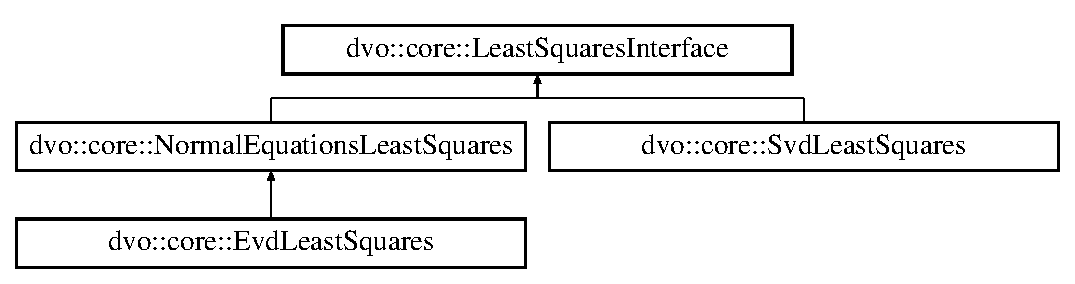
\includegraphics[height=3.000000cm]{classdvo_1_1core_1_1_least_squares_interface}
\end{center}
\end{figure}
\subsection*{Public Member Functions}
\begin{DoxyCompactItemize}
\item 
virtual \mbox{\hyperlink{classdvo_1_1core_1_1_least_squares_interface_afa584f0c27bbcf40a748d678b5295325}{$\sim$\+Least\+Squares\+Interface}} ()
\item 
virtual void \mbox{\hyperlink{classdvo_1_1core_1_1_least_squares_interface_a09e5784f74d7352a9550a8aa523d30d7}{initialize}} (const size\+\_\+t maxnum\+\_\+constraints)=0
\item 
virtual void \mbox{\hyperlink{classdvo_1_1core_1_1_least_squares_interface_a5f5cc1c312a01ff4e7ca91e90a73ccf3}{update}} (const \mbox{\hyperlink{namespacedvo_1_1core_a05327f3312d32a301bce9fccda9e5807}{Vector6}} \&J, const \mbox{\hyperlink{namespacedvo_1_1core_ab9c199d221775a923e2549ad7e15c323}{Num\+Type}} \&res, const \mbox{\hyperlink{namespacedvo_1_1core_ab9c199d221775a923e2549ad7e15c323}{Num\+Type}} \&weight=1.\+0f)=0
\item 
virtual void \mbox{\hyperlink{classdvo_1_1core_1_1_least_squares_interface_a2e580a70e96f0e7d6d70f6047891a42a}{finish}} ()=0
\item 
virtual void \mbox{\hyperlink{classdvo_1_1core_1_1_least_squares_interface_a3e2b3c894c5286fdee79316e6fa4d691}{solve}} (\mbox{\hyperlink{namespacedvo_1_1core_a05327f3312d32a301bce9fccda9e5807}{Vector6}} \&x)=0
\end{DoxyCompactItemize}


\subsection{Detailed Description}
Basic interface for algorithms solving 1 step of non-\/linear least squares. 

\subsection{Constructor \& Destructor Documentation}
\mbox{\Hypertarget{classdvo_1_1core_1_1_least_squares_interface_afa584f0c27bbcf40a748d678b5295325}\label{classdvo_1_1core_1_1_least_squares_interface_afa584f0c27bbcf40a748d678b5295325}} 
\index{dvo\+::core\+::\+Least\+Squares\+Interface@{dvo\+::core\+::\+Least\+Squares\+Interface}!````~Least\+Squares\+Interface@{$\sim$\+Least\+Squares\+Interface}}
\index{````~Least\+Squares\+Interface@{$\sim$\+Least\+Squares\+Interface}!dvo\+::core\+::\+Least\+Squares\+Interface@{dvo\+::core\+::\+Least\+Squares\+Interface}}
\subsubsection{\texorpdfstring{$\sim$\+Least\+Squares\+Interface()}{~LeastSquaresInterface()}}
{\footnotesize\ttfamily virtual dvo\+::core\+::\+Least\+Squares\+Interface\+::$\sim$\+Least\+Squares\+Interface (\begin{DoxyParamCaption}{ }\end{DoxyParamCaption})\hspace{0.3cm}{\ttfamily [inline]}, {\ttfamily [virtual]}}



\subsection{Member Function Documentation}
\mbox{\Hypertarget{classdvo_1_1core_1_1_least_squares_interface_a2e580a70e96f0e7d6d70f6047891a42a}\label{classdvo_1_1core_1_1_least_squares_interface_a2e580a70e96f0e7d6d70f6047891a42a}} 
\index{dvo\+::core\+::\+Least\+Squares\+Interface@{dvo\+::core\+::\+Least\+Squares\+Interface}!finish@{finish}}
\index{finish@{finish}!dvo\+::core\+::\+Least\+Squares\+Interface@{dvo\+::core\+::\+Least\+Squares\+Interface}}
\subsubsection{\texorpdfstring{finish()}{finish()}}
{\footnotesize\ttfamily virtual void dvo\+::core\+::\+Least\+Squares\+Interface\+::finish (\begin{DoxyParamCaption}{ }\end{DoxyParamCaption})\hspace{0.3cm}{\ttfamily [pure virtual]}}



Implemented in \mbox{\hyperlink{classdvo_1_1core_1_1_svd_least_squares_ac91cb5c82af6eb9d91d3ef4e85dc76a3}{dvo\+::core\+::\+Svd\+Least\+Squares}}, and \mbox{\hyperlink{classdvo_1_1core_1_1_normal_equations_least_squares_a0da5301414f684b8e3ebfa9c4794af31}{dvo\+::core\+::\+Normal\+Equations\+Least\+Squares}}.

\mbox{\Hypertarget{classdvo_1_1core_1_1_least_squares_interface_a09e5784f74d7352a9550a8aa523d30d7}\label{classdvo_1_1core_1_1_least_squares_interface_a09e5784f74d7352a9550a8aa523d30d7}} 
\index{dvo\+::core\+::\+Least\+Squares\+Interface@{dvo\+::core\+::\+Least\+Squares\+Interface}!initialize@{initialize}}
\index{initialize@{initialize}!dvo\+::core\+::\+Least\+Squares\+Interface@{dvo\+::core\+::\+Least\+Squares\+Interface}}
\subsubsection{\texorpdfstring{initialize()}{initialize()}}
{\footnotesize\ttfamily virtual void dvo\+::core\+::\+Least\+Squares\+Interface\+::initialize (\begin{DoxyParamCaption}\item[{const size\+\_\+t}]{maxnum\+\_\+constraints }\end{DoxyParamCaption})\hspace{0.3cm}{\ttfamily [pure virtual]}}



Implemented in \mbox{\hyperlink{classdvo_1_1core_1_1_svd_least_squares_aa09756d97cb63e8dc8276a88a1a07791}{dvo\+::core\+::\+Svd\+Least\+Squares}}, and \mbox{\hyperlink{classdvo_1_1core_1_1_normal_equations_least_squares_a4799d66e3dc176ab07418fc1cfacfb53}{dvo\+::core\+::\+Normal\+Equations\+Least\+Squares}}.

\mbox{\Hypertarget{classdvo_1_1core_1_1_least_squares_interface_a3e2b3c894c5286fdee79316e6fa4d691}\label{classdvo_1_1core_1_1_least_squares_interface_a3e2b3c894c5286fdee79316e6fa4d691}} 
\index{dvo\+::core\+::\+Least\+Squares\+Interface@{dvo\+::core\+::\+Least\+Squares\+Interface}!solve@{solve}}
\index{solve@{solve}!dvo\+::core\+::\+Least\+Squares\+Interface@{dvo\+::core\+::\+Least\+Squares\+Interface}}
\subsubsection{\texorpdfstring{solve()}{solve()}}
{\footnotesize\ttfamily virtual void dvo\+::core\+::\+Least\+Squares\+Interface\+::solve (\begin{DoxyParamCaption}\item[{\mbox{\hyperlink{namespacedvo_1_1core_a05327f3312d32a301bce9fccda9e5807}{Vector6}} \&}]{x }\end{DoxyParamCaption})\hspace{0.3cm}{\ttfamily [pure virtual]}}



Implemented in \mbox{\hyperlink{classdvo_1_1core_1_1_svd_least_squares_ae0124d7c24b90b1101bf38da59f789aa}{dvo\+::core\+::\+Svd\+Least\+Squares}}, \mbox{\hyperlink{classdvo_1_1core_1_1_evd_least_squares_a7264139b3006d803039707c4318d2451}{dvo\+::core\+::\+Evd\+Least\+Squares}}, and \mbox{\hyperlink{classdvo_1_1core_1_1_normal_equations_least_squares_a8a25d3970f6506df2066995f2f2effda}{dvo\+::core\+::\+Normal\+Equations\+Least\+Squares}}.

\mbox{\Hypertarget{classdvo_1_1core_1_1_least_squares_interface_a5f5cc1c312a01ff4e7ca91e90a73ccf3}\label{classdvo_1_1core_1_1_least_squares_interface_a5f5cc1c312a01ff4e7ca91e90a73ccf3}} 
\index{dvo\+::core\+::\+Least\+Squares\+Interface@{dvo\+::core\+::\+Least\+Squares\+Interface}!update@{update}}
\index{update@{update}!dvo\+::core\+::\+Least\+Squares\+Interface@{dvo\+::core\+::\+Least\+Squares\+Interface}}
\subsubsection{\texorpdfstring{update()}{update()}}
{\footnotesize\ttfamily virtual void dvo\+::core\+::\+Least\+Squares\+Interface\+::update (\begin{DoxyParamCaption}\item[{const \mbox{\hyperlink{namespacedvo_1_1core_a05327f3312d32a301bce9fccda9e5807}{Vector6}} \&}]{J,  }\item[{const \mbox{\hyperlink{namespacedvo_1_1core_ab9c199d221775a923e2549ad7e15c323}{Num\+Type}} \&}]{res,  }\item[{const \mbox{\hyperlink{namespacedvo_1_1core_ab9c199d221775a923e2549ad7e15c323}{Num\+Type}} \&}]{weight = {\ttfamily 1.0f} }\end{DoxyParamCaption})\hspace{0.3cm}{\ttfamily [pure virtual]}}



Implemented in \mbox{\hyperlink{classdvo_1_1core_1_1_svd_least_squares_ae9d28bc58804d7e43cf461ca092b9563}{dvo\+::core\+::\+Svd\+Least\+Squares}}, and \mbox{\hyperlink{classdvo_1_1core_1_1_normal_equations_least_squares_a1ef767b22d889c99850b1b2dd8cd870d}{dvo\+::core\+::\+Normal\+Equations\+Least\+Squares}}.



The documentation for this class was generated from the following file\+:\begin{DoxyCompactItemize}
\item 
dvo\+\_\+core/include/dvo/core/\mbox{\hyperlink{least__squares_8h}{least\+\_\+squares.\+h}}\end{DoxyCompactItemize}

\hypertarget{classdvo_1_1core_1_1_m_a_d_scale_estimator}{}\section{dvo\+:\+:core\+:\+:M\+A\+D\+Scale\+Estimator Class Reference}
\label{classdvo_1_1core_1_1_m_a_d_scale_estimator}\index{dvo\+::core\+::\+M\+A\+D\+Scale\+Estimator@{dvo\+::core\+::\+M\+A\+D\+Scale\+Estimator}}


{\ttfamily \#include $<$weight\+\_\+calculation.\+h$>$}

Inheritance diagram for dvo\+:\+:core\+:\+:M\+A\+D\+Scale\+Estimator\+:\begin{figure}[H]
\begin{center}
\leavevmode
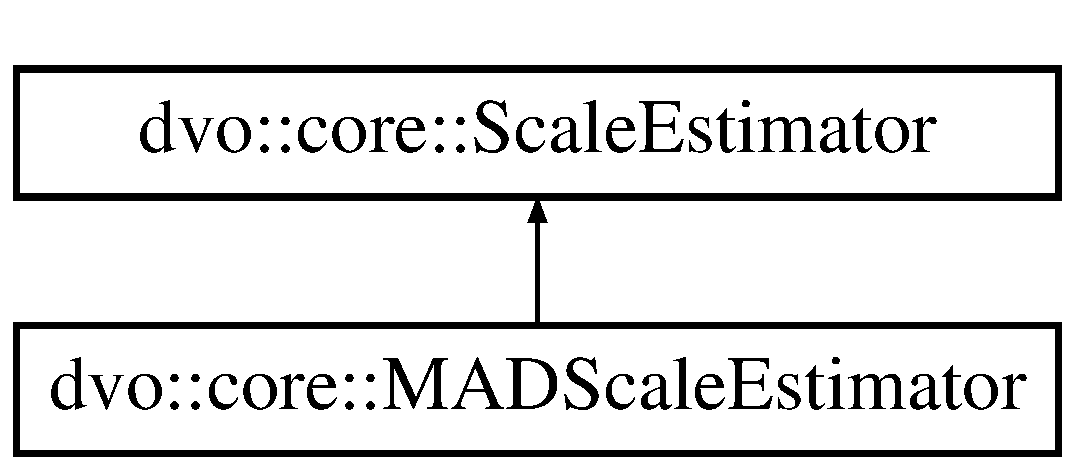
\includegraphics[height=2.000000cm]{classdvo_1_1core_1_1_m_a_d_scale_estimator}
\end{center}
\end{figure}
\subsection*{Public Member Functions}
\begin{DoxyCompactItemize}
\item 
\mbox{\hyperlink{classdvo_1_1core_1_1_m_a_d_scale_estimator_a63a14a6ff40fcc659ceabbac3b229257}{M\+A\+D\+Scale\+Estimator}} ()
\item 
virtual \mbox{\hyperlink{classdvo_1_1core_1_1_m_a_d_scale_estimator_a8192c59f11b969eec2179abe8dc176b5}{$\sim$\+M\+A\+D\+Scale\+Estimator}} ()
\item 
virtual float \mbox{\hyperlink{classdvo_1_1core_1_1_m_a_d_scale_estimator_a421acf5af118ef5b9c394cfd5fadea1d}{compute}} (const cv\+::\+Mat \&errors) const
\end{DoxyCompactItemize}


\subsection{Constructor \& Destructor Documentation}
\mbox{\Hypertarget{classdvo_1_1core_1_1_m_a_d_scale_estimator_a63a14a6ff40fcc659ceabbac3b229257}\label{classdvo_1_1core_1_1_m_a_d_scale_estimator_a63a14a6ff40fcc659ceabbac3b229257}} 
\index{dvo\+::core\+::\+M\+A\+D\+Scale\+Estimator@{dvo\+::core\+::\+M\+A\+D\+Scale\+Estimator}!M\+A\+D\+Scale\+Estimator@{M\+A\+D\+Scale\+Estimator}}
\index{M\+A\+D\+Scale\+Estimator@{M\+A\+D\+Scale\+Estimator}!dvo\+::core\+::\+M\+A\+D\+Scale\+Estimator@{dvo\+::core\+::\+M\+A\+D\+Scale\+Estimator}}
\subsubsection{\texorpdfstring{M\+A\+D\+Scale\+Estimator()}{MADScaleEstimator()}}
{\footnotesize\ttfamily dvo\+::core\+::\+M\+A\+D\+Scale\+Estimator\+::\+M\+A\+D\+Scale\+Estimator (\begin{DoxyParamCaption}{ }\end{DoxyParamCaption})}

\mbox{\Hypertarget{classdvo_1_1core_1_1_m_a_d_scale_estimator_a8192c59f11b969eec2179abe8dc176b5}\label{classdvo_1_1core_1_1_m_a_d_scale_estimator_a8192c59f11b969eec2179abe8dc176b5}} 
\index{dvo\+::core\+::\+M\+A\+D\+Scale\+Estimator@{dvo\+::core\+::\+M\+A\+D\+Scale\+Estimator}!````~M\+A\+D\+Scale\+Estimator@{$\sim$\+M\+A\+D\+Scale\+Estimator}}
\index{````~M\+A\+D\+Scale\+Estimator@{$\sim$\+M\+A\+D\+Scale\+Estimator}!dvo\+::core\+::\+M\+A\+D\+Scale\+Estimator@{dvo\+::core\+::\+M\+A\+D\+Scale\+Estimator}}
\subsubsection{\texorpdfstring{$\sim$\+M\+A\+D\+Scale\+Estimator()}{~MADScaleEstimator()}}
{\footnotesize\ttfamily virtual dvo\+::core\+::\+M\+A\+D\+Scale\+Estimator\+::$\sim$\+M\+A\+D\+Scale\+Estimator (\begin{DoxyParamCaption}{ }\end{DoxyParamCaption})\hspace{0.3cm}{\ttfamily [inline]}, {\ttfamily [virtual]}}



\subsection{Member Function Documentation}
\mbox{\Hypertarget{classdvo_1_1core_1_1_m_a_d_scale_estimator_a421acf5af118ef5b9c394cfd5fadea1d}\label{classdvo_1_1core_1_1_m_a_d_scale_estimator_a421acf5af118ef5b9c394cfd5fadea1d}} 
\index{dvo\+::core\+::\+M\+A\+D\+Scale\+Estimator@{dvo\+::core\+::\+M\+A\+D\+Scale\+Estimator}!compute@{compute}}
\index{compute@{compute}!dvo\+::core\+::\+M\+A\+D\+Scale\+Estimator@{dvo\+::core\+::\+M\+A\+D\+Scale\+Estimator}}
\subsubsection{\texorpdfstring{compute()}{compute()}}
{\footnotesize\ttfamily float dvo\+::core\+::\+M\+A\+D\+Scale\+Estimator\+::compute (\begin{DoxyParamCaption}\item[{const cv\+::\+Mat \&}]{errors }\end{DoxyParamCaption}) const\hspace{0.3cm}{\ttfamily [virtual]}}



Implements \mbox{\hyperlink{classdvo_1_1core_1_1_scale_estimator_a6968ac2cd37c2ce1c966f0c9e17d1a3c}{dvo\+::core\+::\+Scale\+Estimator}}.



The documentation for this class was generated from the following files\+:\begin{DoxyCompactItemize}
\item 
dvo\+\_\+core/include/dvo/core/\mbox{\hyperlink{weight__calculation_8h}{weight\+\_\+calculation.\+h}}\item 
dvo\+\_\+core/src/core/\mbox{\hyperlink{weight__calculation_8cpp}{weight\+\_\+calculation.\+cpp}}\end{DoxyCompactItemize}

\hypertarget{classdvo_1_1core_1_1_math_sse}{}\section{dvo\+:\+:core\+:\+:Math\+Sse$<$ Enabled, Num\+Type $>$ Class Template Reference}
\label{classdvo_1_1core_1_1_math_sse}\index{dvo\+::core\+::\+Math\+Sse$<$ Enabled, Num\+Type $>$@{dvo\+::core\+::\+Math\+Sse$<$ Enabled, Num\+Type $>$}}


{\ttfamily \#include $<$math\+\_\+sse.\+h$>$}

\subsection*{Public Member Functions}
\begin{DoxyCompactItemize}
\item 
{\footnotesize template$<$$>$ }\\void \mbox{\hyperlink{classdvo_1_1core_1_1_math_sse_a5d8a137703df78832e1cfb591b290cb0}{add\+Outer\+Product}} (Eigen\+::\+Matrix$<$ float, 6, 6 $>$ \&mat, const Eigen\+::\+Matrix$<$ float, 6, 1 $>$ \&vec, const float \&scale)
\item 
{\footnotesize template$<$$>$ }\\void \mbox{\hyperlink{classdvo_1_1core_1_1_math_sse_a8403622e21ba348610e4ca96d7c1915c}{add\+Outer\+Product}} (Eigen\+::\+Matrix$<$ double, 6, 6 $>$ \&mat, const Eigen\+::\+Matrix$<$ double, 6, 1 $>$ \&vec, const double \&scale)
\item 
{\footnotesize template$<$$>$ }\\void \mbox{\hyperlink{classdvo_1_1core_1_1_math_sse_a942e37dc174d6ed03a48fcb9e9b53b88}{add}} (Eigen\+::\+Matrix$<$ float, 6, 1 $>$ \&vec, const Eigen\+::\+Matrix$<$ float, 6, 1 $>$ \&other, const float \&scale)
\item 
{\footnotesize template$<$$>$ }\\void \mbox{\hyperlink{classdvo_1_1core_1_1_math_sse_a569d441b55c932cf1220a93ef5f155f3}{add}} (Eigen\+::\+Matrix$<$ double, 6, 1 $>$ \&vec, const Eigen\+::\+Matrix$<$ double, 6, 1 $>$ \&other, const double \&scale)
\item 
{\footnotesize template$<$$>$ }\\void \mbox{\hyperlink{classdvo_1_1core_1_1_math_sse_a5d8a137703df78832e1cfb591b290cb0}{add\+Outer\+Product}} (Eigen\+::\+Matrix$<$ float, 6, 6 $>$ \&mat, const Eigen\+::\+Matrix$<$ float, 6, 1 $>$ \&vec, const float \&scale)
\item 
{\footnotesize template$<$$>$ }\\void \mbox{\hyperlink{classdvo_1_1core_1_1_math_sse_a8403622e21ba348610e4ca96d7c1915c}{add\+Outer\+Product}} (Eigen\+::\+Matrix$<$ double, 6, 6 $>$ \&mat, const Eigen\+::\+Matrix$<$ double, 6, 1 $>$ \&vec, const double \&scale)
\item 
{\footnotesize template$<$$>$ }\\void \mbox{\hyperlink{classdvo_1_1core_1_1_math_sse_a942e37dc174d6ed03a48fcb9e9b53b88}{add}} (Eigen\+::\+Matrix$<$ float, 6, 1 $>$ \&vec, const Eigen\+::\+Matrix$<$ float, 6, 1 $>$ \&other, const float \&scale)
\item 
{\footnotesize template$<$$>$ }\\void \mbox{\hyperlink{classdvo_1_1core_1_1_math_sse_a569d441b55c932cf1220a93ef5f155f3}{add}} (Eigen\+::\+Matrix$<$ double, 6, 1 $>$ \&vec, const Eigen\+::\+Matrix$<$ double, 6, 1 $>$ \&other, const double \&scale)
\end{DoxyCompactItemize}
\subsection*{Static Public Member Functions}
\begin{DoxyCompactItemize}
\item 
static void \mbox{\hyperlink{classdvo_1_1core_1_1_math_sse_af3aa0fc81f7709b6f12e3d771741e469}{add\+Outer\+Product}} (Eigen\+::\+Matrix$<$ \mbox{\hyperlink{namespacedvo_1_1core_ab9c199d221775a923e2549ad7e15c323}{Num\+Type}}, 6, 6 $>$ \&mat, const Eigen\+::\+Matrix$<$ \mbox{\hyperlink{namespacedvo_1_1core_ab9c199d221775a923e2549ad7e15c323}{Num\+Type}}, 6, 1 $>$ \&vec, const \mbox{\hyperlink{namespacedvo_1_1core_ab9c199d221775a923e2549ad7e15c323}{Num\+Type}} \&scale)
\item 
static void \mbox{\hyperlink{classdvo_1_1core_1_1_math_sse_a762ff763ee60cc18d6e5bc9197b601a5}{add}} (Eigen\+::\+Matrix$<$ \mbox{\hyperlink{namespacedvo_1_1core_ab9c199d221775a923e2549ad7e15c323}{Num\+Type}}, 6, 1 $>$ \&vec, const Eigen\+::\+Matrix$<$ \mbox{\hyperlink{namespacedvo_1_1core_ab9c199d221775a923e2549ad7e15c323}{Num\+Type}}, 6, 1 $>$ \&other, const \mbox{\hyperlink{namespacedvo_1_1core_ab9c199d221775a923e2549ad7e15c323}{Num\+Type}} \&scale)
\end{DoxyCompactItemize}


\subsection{Member Function Documentation}
\mbox{\Hypertarget{classdvo_1_1core_1_1_math_sse_a762ff763ee60cc18d6e5bc9197b601a5}\label{classdvo_1_1core_1_1_math_sse_a762ff763ee60cc18d6e5bc9197b601a5}} 
\index{dvo\+::core\+::\+Math\+Sse@{dvo\+::core\+::\+Math\+Sse}!add@{add}}
\index{add@{add}!dvo\+::core\+::\+Math\+Sse@{dvo\+::core\+::\+Math\+Sse}}
\subsubsection{\texorpdfstring{add()}{add()}\hspace{0.1cm}{\footnotesize\ttfamily [1/5]}}
{\footnotesize\ttfamily template$<$int Enabled, typename Num\+Type $>$ \\
static void \mbox{\hyperlink{classdvo_1_1core_1_1_math_sse}{dvo\+::core\+::\+Math\+Sse}}$<$ Enabled, \mbox{\hyperlink{namespacedvo_1_1core_ab9c199d221775a923e2549ad7e15c323}{Num\+Type}} $>$\+::add (\begin{DoxyParamCaption}\item[{Eigen\+::\+Matrix$<$ \mbox{\hyperlink{namespacedvo_1_1core_ab9c199d221775a923e2549ad7e15c323}{Num\+Type}}, 6, 1 $>$ \&}]{vec,  }\item[{const Eigen\+::\+Matrix$<$ \mbox{\hyperlink{namespacedvo_1_1core_ab9c199d221775a923e2549ad7e15c323}{Num\+Type}}, 6, 1 $>$ \&}]{other,  }\item[{const \mbox{\hyperlink{namespacedvo_1_1core_ab9c199d221775a923e2549ad7e15c323}{Num\+Type}} \&}]{scale }\end{DoxyParamCaption})\hspace{0.3cm}{\ttfamily [static]}}

\mbox{\Hypertarget{classdvo_1_1core_1_1_math_sse_a942e37dc174d6ed03a48fcb9e9b53b88}\label{classdvo_1_1core_1_1_math_sse_a942e37dc174d6ed03a48fcb9e9b53b88}} 
\index{dvo\+::core\+::\+Math\+Sse@{dvo\+::core\+::\+Math\+Sse}!add@{add}}
\index{add@{add}!dvo\+::core\+::\+Math\+Sse@{dvo\+::core\+::\+Math\+Sse}}
\subsubsection{\texorpdfstring{add()}{add()}\hspace{0.1cm}{\footnotesize\ttfamily [2/5]}}
{\footnotesize\ttfamily template$<$$>$ \\
void \mbox{\hyperlink{classdvo_1_1core_1_1_math_sse}{dvo\+::core\+::\+Math\+Sse}}$<$ \mbox{\hyperlink{structdvo_1_1core_1_1_sse_a4fd9b55a1ec035f837cc78f33d45a9adadefbacd4d80d2e8ba64c1583a4fda95a}{Sse\+::\+Enabled}}, float $>$\+::add (\begin{DoxyParamCaption}\item[{Eigen\+::\+Matrix$<$ float, 6, 1 $>$ \&}]{vec,  }\item[{const Eigen\+::\+Matrix$<$ float, 6, 1 $>$ \&}]{other,  }\item[{const float \&}]{scale }\end{DoxyParamCaption})}

\mbox{\Hypertarget{classdvo_1_1core_1_1_math_sse_a569d441b55c932cf1220a93ef5f155f3}\label{classdvo_1_1core_1_1_math_sse_a569d441b55c932cf1220a93ef5f155f3}} 
\index{dvo\+::core\+::\+Math\+Sse@{dvo\+::core\+::\+Math\+Sse}!add@{add}}
\index{add@{add}!dvo\+::core\+::\+Math\+Sse@{dvo\+::core\+::\+Math\+Sse}}
\subsubsection{\texorpdfstring{add()}{add()}\hspace{0.1cm}{\footnotesize\ttfamily [3/5]}}
{\footnotesize\ttfamily template$<$$>$ \\
void \mbox{\hyperlink{classdvo_1_1core_1_1_math_sse}{dvo\+::core\+::\+Math\+Sse}}$<$ \mbox{\hyperlink{structdvo_1_1core_1_1_sse_a4fd9b55a1ec035f837cc78f33d45a9adadefbacd4d80d2e8ba64c1583a4fda95a}{Sse\+::\+Enabled}}, double $>$\+::add (\begin{DoxyParamCaption}\item[{Eigen\+::\+Matrix$<$ double, 6, 1 $>$ \&}]{vec,  }\item[{const Eigen\+::\+Matrix$<$ double, 6, 1 $>$ \&}]{other,  }\item[{const double \&}]{scale }\end{DoxyParamCaption})}

\mbox{\Hypertarget{classdvo_1_1core_1_1_math_sse_a942e37dc174d6ed03a48fcb9e9b53b88}\label{classdvo_1_1core_1_1_math_sse_a942e37dc174d6ed03a48fcb9e9b53b88}} 
\index{dvo\+::core\+::\+Math\+Sse@{dvo\+::core\+::\+Math\+Sse}!add@{add}}
\index{add@{add}!dvo\+::core\+::\+Math\+Sse@{dvo\+::core\+::\+Math\+Sse}}
\subsubsection{\texorpdfstring{add()}{add()}\hspace{0.1cm}{\footnotesize\ttfamily [4/5]}}
{\footnotesize\ttfamily template$<$$>$ \\
void \mbox{\hyperlink{classdvo_1_1core_1_1_math_sse}{dvo\+::core\+::\+Math\+Sse}}$<$ \mbox{\hyperlink{structdvo_1_1core_1_1_sse_a4fd9b55a1ec035f837cc78f33d45a9adadefbacd4d80d2e8ba64c1583a4fda95a}{Sse\+::\+Enabled}}, float $>$\+::add (\begin{DoxyParamCaption}\item[{Eigen\+::\+Matrix$<$ float, 6, 1 $>$ \&}]{vec,  }\item[{const Eigen\+::\+Matrix$<$ float, 6, 1 $>$ \&}]{other,  }\item[{const float \&}]{scale }\end{DoxyParamCaption})}

\mbox{\Hypertarget{classdvo_1_1core_1_1_math_sse_a569d441b55c932cf1220a93ef5f155f3}\label{classdvo_1_1core_1_1_math_sse_a569d441b55c932cf1220a93ef5f155f3}} 
\index{dvo\+::core\+::\+Math\+Sse@{dvo\+::core\+::\+Math\+Sse}!add@{add}}
\index{add@{add}!dvo\+::core\+::\+Math\+Sse@{dvo\+::core\+::\+Math\+Sse}}
\subsubsection{\texorpdfstring{add()}{add()}\hspace{0.1cm}{\footnotesize\ttfamily [5/5]}}
{\footnotesize\ttfamily template$<$$>$ \\
void \mbox{\hyperlink{classdvo_1_1core_1_1_math_sse}{dvo\+::core\+::\+Math\+Sse}}$<$ \mbox{\hyperlink{structdvo_1_1core_1_1_sse_a4fd9b55a1ec035f837cc78f33d45a9adadefbacd4d80d2e8ba64c1583a4fda95a}{Sse\+::\+Enabled}}, double $>$\+::add (\begin{DoxyParamCaption}\item[{Eigen\+::\+Matrix$<$ double, 6, 1 $>$ \&}]{vec,  }\item[{const Eigen\+::\+Matrix$<$ double, 6, 1 $>$ \&}]{other,  }\item[{const double \&}]{scale }\end{DoxyParamCaption})}

\mbox{\Hypertarget{classdvo_1_1core_1_1_math_sse_af3aa0fc81f7709b6f12e3d771741e469}\label{classdvo_1_1core_1_1_math_sse_af3aa0fc81f7709b6f12e3d771741e469}} 
\index{dvo\+::core\+::\+Math\+Sse@{dvo\+::core\+::\+Math\+Sse}!add\+Outer\+Product@{add\+Outer\+Product}}
\index{add\+Outer\+Product@{add\+Outer\+Product}!dvo\+::core\+::\+Math\+Sse@{dvo\+::core\+::\+Math\+Sse}}
\subsubsection{\texorpdfstring{add\+Outer\+Product()}{addOuterProduct()}\hspace{0.1cm}{\footnotesize\ttfamily [1/5]}}
{\footnotesize\ttfamily template$<$int Enabled, typename Num\+Type $>$ \\
static void \mbox{\hyperlink{classdvo_1_1core_1_1_math_sse}{dvo\+::core\+::\+Math\+Sse}}$<$ Enabled, \mbox{\hyperlink{namespacedvo_1_1core_ab9c199d221775a923e2549ad7e15c323}{Num\+Type}} $>$\+::add\+Outer\+Product (\begin{DoxyParamCaption}\item[{Eigen\+::\+Matrix$<$ \mbox{\hyperlink{namespacedvo_1_1core_ab9c199d221775a923e2549ad7e15c323}{Num\+Type}}, 6, 6 $>$ \&}]{mat,  }\item[{const Eigen\+::\+Matrix$<$ \mbox{\hyperlink{namespacedvo_1_1core_ab9c199d221775a923e2549ad7e15c323}{Num\+Type}}, 6, 1 $>$ \&}]{vec,  }\item[{const \mbox{\hyperlink{namespacedvo_1_1core_ab9c199d221775a923e2549ad7e15c323}{Num\+Type}} \&}]{scale }\end{DoxyParamCaption})\hspace{0.3cm}{\ttfamily [static]}}

\mbox{\Hypertarget{classdvo_1_1core_1_1_math_sse_a5d8a137703df78832e1cfb591b290cb0}\label{classdvo_1_1core_1_1_math_sse_a5d8a137703df78832e1cfb591b290cb0}} 
\index{dvo\+::core\+::\+Math\+Sse@{dvo\+::core\+::\+Math\+Sse}!add\+Outer\+Product@{add\+Outer\+Product}}
\index{add\+Outer\+Product@{add\+Outer\+Product}!dvo\+::core\+::\+Math\+Sse@{dvo\+::core\+::\+Math\+Sse}}
\subsubsection{\texorpdfstring{add\+Outer\+Product()}{addOuterProduct()}\hspace{0.1cm}{\footnotesize\ttfamily [2/5]}}
{\footnotesize\ttfamily template$<$$>$ \\
void \mbox{\hyperlink{classdvo_1_1core_1_1_math_sse}{dvo\+::core\+::\+Math\+Sse}}$<$ \mbox{\hyperlink{structdvo_1_1core_1_1_sse_a4fd9b55a1ec035f837cc78f33d45a9adadefbacd4d80d2e8ba64c1583a4fda95a}{Sse\+::\+Enabled}}, float $>$\+::add\+Outer\+Product (\begin{DoxyParamCaption}\item[{Eigen\+::\+Matrix$<$ float, 6, 6 $>$ \&}]{mat,  }\item[{const Eigen\+::\+Matrix$<$ float, 6, 1 $>$ \&}]{vec,  }\item[{const float \&}]{scale }\end{DoxyParamCaption})}

\mbox{\Hypertarget{classdvo_1_1core_1_1_math_sse_a5d8a137703df78832e1cfb591b290cb0}\label{classdvo_1_1core_1_1_math_sse_a5d8a137703df78832e1cfb591b290cb0}} 
\index{dvo\+::core\+::\+Math\+Sse@{dvo\+::core\+::\+Math\+Sse}!add\+Outer\+Product@{add\+Outer\+Product}}
\index{add\+Outer\+Product@{add\+Outer\+Product}!dvo\+::core\+::\+Math\+Sse@{dvo\+::core\+::\+Math\+Sse}}
\subsubsection{\texorpdfstring{add\+Outer\+Product()}{addOuterProduct()}\hspace{0.1cm}{\footnotesize\ttfamily [3/5]}}
{\footnotesize\ttfamily template$<$$>$ \\
void \mbox{\hyperlink{classdvo_1_1core_1_1_math_sse}{dvo\+::core\+::\+Math\+Sse}}$<$ \mbox{\hyperlink{structdvo_1_1core_1_1_sse_a4fd9b55a1ec035f837cc78f33d45a9adadefbacd4d80d2e8ba64c1583a4fda95a}{Sse\+::\+Enabled}}, float $>$\+::add\+Outer\+Product (\begin{DoxyParamCaption}\item[{Eigen\+::\+Matrix$<$ float, 6, 6 $>$ \&}]{mat,  }\item[{const Eigen\+::\+Matrix$<$ float, 6, 1 $>$ \&}]{vec,  }\item[{const float \&}]{scale }\end{DoxyParamCaption})}

idea\+:

vec = \mbox{[}j0 j1 j2 j3 j4 j5\mbox{]}

vec $\ast$ vec.\+transpose() = \mbox{[} j0$\ast$j0 j0$\ast$j1 j0$\ast$j2 j0$\ast$j3 j0$\ast$j4 j0$\ast$j5 j1$\ast$j0 j1$\ast$j1 j1$\ast$j2 j1$\ast$j3 j1$\ast$j4 j1$\ast$j5 j2$\ast$j0 j2$\ast$j1 j2$\ast$j2 j2$\ast$j3 j2$\ast$j4 j2$\ast$j5 j3$\ast$j0 j3$\ast$j1 j3$\ast$j2 j3$\ast$j3 j3$\ast$j4 j3$\ast$j5 j4$\ast$j0 j4$\ast$j1 j4$\ast$j2 j4$\ast$j3 j4$\ast$j4 j4$\ast$j5 j5$\ast$j0 j5$\ast$j1 j5$\ast$j2 j5$\ast$j3 j5$\ast$j4 j5$\ast$j5 \mbox{]}

row multiplicators\+:

j0 $\ast$ \mbox{[}j0 j1 j2 j3 j4 j5\mbox{]} j1 $\ast$ \mbox{[}j0 j1 j2 j3 j4 j5\mbox{]} j2 $\ast$ \mbox{[}j0 j1 j2 j3 j4 j5\mbox{]} j3 $\ast$ \mbox{[}j0 j1 j2 j3 j4 j5\mbox{]} j4 $\ast$ \mbox{[}j0 j1 j2 j3 j4 j5\mbox{]} j5 $\ast$ \mbox{[}j0 j1 j2 j3 j4 j5\mbox{]}

substitute\+:

v1 = \mbox{[}j0 j1 j2 j3\mbox{]}, v2 = \mbox{[}j4 j5 j0 j1\mbox{]}, v3 = \mbox{[}j2 j3 j4 j5\mbox{]}

calculate\+:

\mbox{[}j0 j0 j0 j0\mbox{]} $\ast$ v1, \mbox{[}j0 j0 j1 j1\mbox{]} $\ast$ v2, \mbox{[}j1 j1 j1 j1\mbox{]} $\ast$ v3 \mbox{[}j2 j2 j2 j2\mbox{]} $\ast$ v1, \mbox{[}j2 j2 j3 j3\mbox{]} $\ast$ v2, \mbox{[}j3 j3 j3 j3\mbox{]} $\ast$ v3 \mbox{[}j4 j4 j4 j4\mbox{]} $\ast$ v1, \mbox{[}j4 j4 j5 j5\mbox{]} $\ast$ v2, \mbox{[}j5 j5 j5 j5\mbox{]} $\ast$ v3

the vectors for multiplication can be obtained by shuffling v1 and v2 (they are prescaled with scale to v1s and v2s)

after each multiplication add result to matrix\mbox{\Hypertarget{classdvo_1_1core_1_1_math_sse_a8403622e21ba348610e4ca96d7c1915c}\label{classdvo_1_1core_1_1_math_sse_a8403622e21ba348610e4ca96d7c1915c}} 
\index{dvo\+::core\+::\+Math\+Sse@{dvo\+::core\+::\+Math\+Sse}!add\+Outer\+Product@{add\+Outer\+Product}}
\index{add\+Outer\+Product@{add\+Outer\+Product}!dvo\+::core\+::\+Math\+Sse@{dvo\+::core\+::\+Math\+Sse}}
\subsubsection{\texorpdfstring{add\+Outer\+Product()}{addOuterProduct()}\hspace{0.1cm}{\footnotesize\ttfamily [4/5]}}
{\footnotesize\ttfamily template$<$$>$ \\
void \mbox{\hyperlink{classdvo_1_1core_1_1_math_sse}{dvo\+::core\+::\+Math\+Sse}}$<$ \mbox{\hyperlink{structdvo_1_1core_1_1_sse_a4fd9b55a1ec035f837cc78f33d45a9adadefbacd4d80d2e8ba64c1583a4fda95a}{Sse\+::\+Enabled}}, double $>$\+::add\+Outer\+Product (\begin{DoxyParamCaption}\item[{Eigen\+::\+Matrix$<$ double, 6, 6 $>$ \&}]{mat,  }\item[{const Eigen\+::\+Matrix$<$ double, 6, 1 $>$ \&}]{vec,  }\item[{const double \&}]{scale }\end{DoxyParamCaption})}

\mbox{\Hypertarget{classdvo_1_1core_1_1_math_sse_a8403622e21ba348610e4ca96d7c1915c}\label{classdvo_1_1core_1_1_math_sse_a8403622e21ba348610e4ca96d7c1915c}} 
\index{dvo\+::core\+::\+Math\+Sse@{dvo\+::core\+::\+Math\+Sse}!add\+Outer\+Product@{add\+Outer\+Product}}
\index{add\+Outer\+Product@{add\+Outer\+Product}!dvo\+::core\+::\+Math\+Sse@{dvo\+::core\+::\+Math\+Sse}}
\subsubsection{\texorpdfstring{add\+Outer\+Product()}{addOuterProduct()}\hspace{0.1cm}{\footnotesize\ttfamily [5/5]}}
{\footnotesize\ttfamily template$<$$>$ \\
void \mbox{\hyperlink{classdvo_1_1core_1_1_math_sse}{dvo\+::core\+::\+Math\+Sse}}$<$ \mbox{\hyperlink{structdvo_1_1core_1_1_sse_a4fd9b55a1ec035f837cc78f33d45a9adadefbacd4d80d2e8ba64c1583a4fda95a}{Sse\+::\+Enabled}}, double $>$\+::add\+Outer\+Product (\begin{DoxyParamCaption}\item[{Eigen\+::\+Matrix$<$ double, 6, 6 $>$ \&}]{mat,  }\item[{const Eigen\+::\+Matrix$<$ double, 6, 1 $>$ \&}]{vec,  }\item[{const double \&}]{scale }\end{DoxyParamCaption})}



The documentation for this class was generated from the following file\+:\begin{DoxyCompactItemize}
\item 
dvo\+\_\+core/include/dvo/core/\mbox{\hyperlink{math__sse_8h}{math\+\_\+sse.\+h}}\end{DoxyCompactItemize}

\hypertarget{classdvo_1_1core_1_1_math_sse_3_01_sse_1_1_disabled_00_01_num_type_01_4}{}\section{dvo\+:\+:core\+:\+:Math\+Sse$<$ Sse\+:\+:Disabled, Num\+Type $>$ Class Template Reference}
\label{classdvo_1_1core_1_1_math_sse_3_01_sse_1_1_disabled_00_01_num_type_01_4}\index{dvo\+::core\+::\+Math\+Sse$<$ Sse\+::\+Disabled, Num\+Type $>$@{dvo\+::core\+::\+Math\+Sse$<$ Sse\+::\+Disabled, Num\+Type $>$}}


{\ttfamily \#include $<$math\+\_\+sse.\+h$>$}

\subsection*{Static Public Member Functions}
\begin{DoxyCompactItemize}
\item 
static void \mbox{\hyperlink{classdvo_1_1core_1_1_math_sse_3_01_sse_1_1_disabled_00_01_num_type_01_4_ad8e43368f340963344f0d87a1a72e070}{add\+Outer\+Product}} (Eigen\+::\+Matrix$<$ \mbox{\hyperlink{namespacedvo_1_1core_ab9c199d221775a923e2549ad7e15c323}{Num\+Type}}, 6, 6 $>$ \&mat, const Eigen\+::\+Matrix$<$ \mbox{\hyperlink{namespacedvo_1_1core_ab9c199d221775a923e2549ad7e15c323}{Num\+Type}}, 6, 1 $>$ \&vec, const \mbox{\hyperlink{namespacedvo_1_1core_ab9c199d221775a923e2549ad7e15c323}{Num\+Type}} \&scale)
\item 
static void \mbox{\hyperlink{classdvo_1_1core_1_1_math_sse_3_01_sse_1_1_disabled_00_01_num_type_01_4_a354a83ac6da90d558363c2394a5b1499}{add}} (Eigen\+::\+Matrix$<$ \mbox{\hyperlink{namespacedvo_1_1core_ab9c199d221775a923e2549ad7e15c323}{Num\+Type}}, 6, 1 $>$ \&vec, const Eigen\+::\+Matrix$<$ \mbox{\hyperlink{namespacedvo_1_1core_ab9c199d221775a923e2549ad7e15c323}{Num\+Type}}, 6, 1 $>$ \&other, const \mbox{\hyperlink{namespacedvo_1_1core_ab9c199d221775a923e2549ad7e15c323}{Num\+Type}} \&scale)
\end{DoxyCompactItemize}


\subsection{Member Function Documentation}
\mbox{\Hypertarget{classdvo_1_1core_1_1_math_sse_3_01_sse_1_1_disabled_00_01_num_type_01_4_a354a83ac6da90d558363c2394a5b1499}\label{classdvo_1_1core_1_1_math_sse_3_01_sse_1_1_disabled_00_01_num_type_01_4_a354a83ac6da90d558363c2394a5b1499}} 
\index{dvo\+::core\+::\+Math\+Sse$<$ Sse\+::\+Disabled, Num\+Type $>$@{dvo\+::core\+::\+Math\+Sse$<$ Sse\+::\+Disabled, Num\+Type $>$}!add@{add}}
\index{add@{add}!dvo\+::core\+::\+Math\+Sse$<$ Sse\+::\+Disabled, Num\+Type $>$@{dvo\+::core\+::\+Math\+Sse$<$ Sse\+::\+Disabled, Num\+Type $>$}}
\subsubsection{\texorpdfstring{add()}{add()}}
{\footnotesize\ttfamily template$<$typename Num\+Type $>$ \\
static void \mbox{\hyperlink{classdvo_1_1core_1_1_math_sse}{dvo\+::core\+::\+Math\+Sse}}$<$ \mbox{\hyperlink{structdvo_1_1core_1_1_sse_a4fd9b55a1ec035f837cc78f33d45a9adaeeb0a9210cb89d05bec4d9b12e628ae3}{Sse\+::\+Disabled}}, \mbox{\hyperlink{namespacedvo_1_1core_ab9c199d221775a923e2549ad7e15c323}{Num\+Type}} $>$\+::add (\begin{DoxyParamCaption}\item[{Eigen\+::\+Matrix$<$ \mbox{\hyperlink{namespacedvo_1_1core_ab9c199d221775a923e2549ad7e15c323}{Num\+Type}}, 6, 1 $>$ \&}]{vec,  }\item[{const Eigen\+::\+Matrix$<$ \mbox{\hyperlink{namespacedvo_1_1core_ab9c199d221775a923e2549ad7e15c323}{Num\+Type}}, 6, 1 $>$ \&}]{other,  }\item[{const \mbox{\hyperlink{namespacedvo_1_1core_ab9c199d221775a923e2549ad7e15c323}{Num\+Type}} \&}]{scale }\end{DoxyParamCaption})\hspace{0.3cm}{\ttfamily [inline]}, {\ttfamily [static]}}

\mbox{\Hypertarget{classdvo_1_1core_1_1_math_sse_3_01_sse_1_1_disabled_00_01_num_type_01_4_ad8e43368f340963344f0d87a1a72e070}\label{classdvo_1_1core_1_1_math_sse_3_01_sse_1_1_disabled_00_01_num_type_01_4_ad8e43368f340963344f0d87a1a72e070}} 
\index{dvo\+::core\+::\+Math\+Sse$<$ Sse\+::\+Disabled, Num\+Type $>$@{dvo\+::core\+::\+Math\+Sse$<$ Sse\+::\+Disabled, Num\+Type $>$}!add\+Outer\+Product@{add\+Outer\+Product}}
\index{add\+Outer\+Product@{add\+Outer\+Product}!dvo\+::core\+::\+Math\+Sse$<$ Sse\+::\+Disabled, Num\+Type $>$@{dvo\+::core\+::\+Math\+Sse$<$ Sse\+::\+Disabled, Num\+Type $>$}}
\subsubsection{\texorpdfstring{add\+Outer\+Product()}{addOuterProduct()}}
{\footnotesize\ttfamily template$<$typename Num\+Type $>$ \\
static void \mbox{\hyperlink{classdvo_1_1core_1_1_math_sse}{dvo\+::core\+::\+Math\+Sse}}$<$ \mbox{\hyperlink{structdvo_1_1core_1_1_sse_a4fd9b55a1ec035f837cc78f33d45a9adaeeb0a9210cb89d05bec4d9b12e628ae3}{Sse\+::\+Disabled}}, \mbox{\hyperlink{namespacedvo_1_1core_ab9c199d221775a923e2549ad7e15c323}{Num\+Type}} $>$\+::add\+Outer\+Product (\begin{DoxyParamCaption}\item[{Eigen\+::\+Matrix$<$ \mbox{\hyperlink{namespacedvo_1_1core_ab9c199d221775a923e2549ad7e15c323}{Num\+Type}}, 6, 6 $>$ \&}]{mat,  }\item[{const Eigen\+::\+Matrix$<$ \mbox{\hyperlink{namespacedvo_1_1core_ab9c199d221775a923e2549ad7e15c323}{Num\+Type}}, 6, 1 $>$ \&}]{vec,  }\item[{const \mbox{\hyperlink{namespacedvo_1_1core_ab9c199d221775a923e2549ad7e15c323}{Num\+Type}} \&}]{scale }\end{DoxyParamCaption})\hspace{0.3cm}{\ttfamily [inline]}, {\ttfamily [static]}}



The documentation for this class was generated from the following file\+:\begin{DoxyCompactItemize}
\item 
dvo\+\_\+core/include/dvo/core/\mbox{\hyperlink{math__sse_8h}{math\+\_\+sse.\+h}}\end{DoxyCompactItemize}

\hypertarget{structdvo_1_1visualization_1_1_visualizer_impl_1_1_named_image}{}\section{dvo\+:\+:visualization\+:\+:Visualizer\+Impl\+:\+:Named\+Image Struct Reference}
\label{structdvo_1_1visualization_1_1_visualizer_impl_1_1_named_image}\index{dvo\+::visualization\+::\+Visualizer\+Impl\+::\+Named\+Image@{dvo\+::visualization\+::\+Visualizer\+Impl\+::\+Named\+Image}}
\subsection*{Public Member Functions}
\begin{DoxyCompactItemize}
\item 
\mbox{\hyperlink{structdvo_1_1visualization_1_1_visualizer_impl_1_1_named_image_ad8d49d26aa2b0fd5166857b2ee913489}{Named\+Image}} ()
\item 
\mbox{\hyperlink{structdvo_1_1visualization_1_1_visualizer_impl_1_1_named_image_a85ef82568b83987428230f90bc4c00a2}{Named\+Image}} (std\+::string \&\mbox{\hyperlink{structdvo_1_1visualization_1_1_visualizer_impl_1_1_named_image_aa46e7e1b17cd744452ba8ef3dffddfe7}{name}}, const cv\+::\+Mat\+Expr \&\mbox{\hyperlink{structdvo_1_1visualization_1_1_visualizer_impl_1_1_named_image_a7ff904dac2fc68f459ee05a32abf3cea}{img}}, \mbox{\hyperlink{classdvo_1_1visualization_1_1_visualizer_ac33e0b53e7ef7be64e3230f6c91084a0}{Visualizer\+::\+Image\+Modifier}} \&\mbox{\hyperlink{structdvo_1_1visualization_1_1_visualizer_impl_1_1_named_image_a831a0937bdfc9427f20669770f37f1d0}{modifier}})
\end{DoxyCompactItemize}
\subsection*{Public Attributes}
\begin{DoxyCompactItemize}
\item 
std\+::string \mbox{\hyperlink{structdvo_1_1visualization_1_1_visualizer_impl_1_1_named_image_aa46e7e1b17cd744452ba8ef3dffddfe7}{name}}
\item 
cv\+::\+Mat\+Expr \mbox{\hyperlink{structdvo_1_1visualization_1_1_visualizer_impl_1_1_named_image_a7ff904dac2fc68f459ee05a32abf3cea}{img}}
\item 
\mbox{\hyperlink{classdvo_1_1visualization_1_1_visualizer_ac33e0b53e7ef7be64e3230f6c91084a0}{Visualizer\+::\+Image\+Modifier}} \mbox{\hyperlink{structdvo_1_1visualization_1_1_visualizer_impl_1_1_named_image_a831a0937bdfc9427f20669770f37f1d0}{modifier}}
\end{DoxyCompactItemize}


\subsection{Constructor \& Destructor Documentation}
\mbox{\Hypertarget{structdvo_1_1visualization_1_1_visualizer_impl_1_1_named_image_ad8d49d26aa2b0fd5166857b2ee913489}\label{structdvo_1_1visualization_1_1_visualizer_impl_1_1_named_image_ad8d49d26aa2b0fd5166857b2ee913489}} 
\index{dvo\+::visualization\+::\+Visualizer\+Impl\+::\+Named\+Image@{dvo\+::visualization\+::\+Visualizer\+Impl\+::\+Named\+Image}!Named\+Image@{Named\+Image}}
\index{Named\+Image@{Named\+Image}!dvo\+::visualization\+::\+Visualizer\+Impl\+::\+Named\+Image@{dvo\+::visualization\+::\+Visualizer\+Impl\+::\+Named\+Image}}
\subsubsection{\texorpdfstring{Named\+Image()}{NamedImage()}\hspace{0.1cm}{\footnotesize\ttfamily [1/2]}}
{\footnotesize\ttfamily dvo\+::visualization\+::\+Visualizer\+Impl\+::\+Named\+Image\+::\+Named\+Image (\begin{DoxyParamCaption}{ }\end{DoxyParamCaption})\hspace{0.3cm}{\ttfamily [inline]}}

\mbox{\Hypertarget{structdvo_1_1visualization_1_1_visualizer_impl_1_1_named_image_a85ef82568b83987428230f90bc4c00a2}\label{structdvo_1_1visualization_1_1_visualizer_impl_1_1_named_image_a85ef82568b83987428230f90bc4c00a2}} 
\index{dvo\+::visualization\+::\+Visualizer\+Impl\+::\+Named\+Image@{dvo\+::visualization\+::\+Visualizer\+Impl\+::\+Named\+Image}!Named\+Image@{Named\+Image}}
\index{Named\+Image@{Named\+Image}!dvo\+::visualization\+::\+Visualizer\+Impl\+::\+Named\+Image@{dvo\+::visualization\+::\+Visualizer\+Impl\+::\+Named\+Image}}
\subsubsection{\texorpdfstring{Named\+Image()}{NamedImage()}\hspace{0.1cm}{\footnotesize\ttfamily [2/2]}}
{\footnotesize\ttfamily dvo\+::visualization\+::\+Visualizer\+Impl\+::\+Named\+Image\+::\+Named\+Image (\begin{DoxyParamCaption}\item[{std\+::string \&}]{name,  }\item[{const cv\+::\+Mat\+Expr \&}]{img,  }\item[{\mbox{\hyperlink{classdvo_1_1visualization_1_1_visualizer_ac33e0b53e7ef7be64e3230f6c91084a0}{Visualizer\+::\+Image\+Modifier}} \&}]{modifier }\end{DoxyParamCaption})\hspace{0.3cm}{\ttfamily [inline]}}



\subsection{Member Data Documentation}
\mbox{\Hypertarget{structdvo_1_1visualization_1_1_visualizer_impl_1_1_named_image_a7ff904dac2fc68f459ee05a32abf3cea}\label{structdvo_1_1visualization_1_1_visualizer_impl_1_1_named_image_a7ff904dac2fc68f459ee05a32abf3cea}} 
\index{dvo\+::visualization\+::\+Visualizer\+Impl\+::\+Named\+Image@{dvo\+::visualization\+::\+Visualizer\+Impl\+::\+Named\+Image}!img@{img}}
\index{img@{img}!dvo\+::visualization\+::\+Visualizer\+Impl\+::\+Named\+Image@{dvo\+::visualization\+::\+Visualizer\+Impl\+::\+Named\+Image}}
\subsubsection{\texorpdfstring{img}{img}}
{\footnotesize\ttfamily cv\+::\+Mat\+Expr dvo\+::visualization\+::\+Visualizer\+Impl\+::\+Named\+Image\+::img}

\mbox{\Hypertarget{structdvo_1_1visualization_1_1_visualizer_impl_1_1_named_image_a831a0937bdfc9427f20669770f37f1d0}\label{structdvo_1_1visualization_1_1_visualizer_impl_1_1_named_image_a831a0937bdfc9427f20669770f37f1d0}} 
\index{dvo\+::visualization\+::\+Visualizer\+Impl\+::\+Named\+Image@{dvo\+::visualization\+::\+Visualizer\+Impl\+::\+Named\+Image}!modifier@{modifier}}
\index{modifier@{modifier}!dvo\+::visualization\+::\+Visualizer\+Impl\+::\+Named\+Image@{dvo\+::visualization\+::\+Visualizer\+Impl\+::\+Named\+Image}}
\subsubsection{\texorpdfstring{modifier}{modifier}}
{\footnotesize\ttfamily \mbox{\hyperlink{classdvo_1_1visualization_1_1_visualizer_ac33e0b53e7ef7be64e3230f6c91084a0}{Visualizer\+::\+Image\+Modifier}} dvo\+::visualization\+::\+Visualizer\+Impl\+::\+Named\+Image\+::modifier}

\mbox{\Hypertarget{structdvo_1_1visualization_1_1_visualizer_impl_1_1_named_image_aa46e7e1b17cd744452ba8ef3dffddfe7}\label{structdvo_1_1visualization_1_1_visualizer_impl_1_1_named_image_aa46e7e1b17cd744452ba8ef3dffddfe7}} 
\index{dvo\+::visualization\+::\+Visualizer\+Impl\+::\+Named\+Image@{dvo\+::visualization\+::\+Visualizer\+Impl\+::\+Named\+Image}!name@{name}}
\index{name@{name}!dvo\+::visualization\+::\+Visualizer\+Impl\+::\+Named\+Image@{dvo\+::visualization\+::\+Visualizer\+Impl\+::\+Named\+Image}}
\subsubsection{\texorpdfstring{name}{name}}
{\footnotesize\ttfamily std\+::string dvo\+::visualization\+::\+Visualizer\+Impl\+::\+Named\+Image\+::name}



The documentation for this struct was generated from the following file\+:\begin{DoxyCompactItemize}
\item 
dvo\+\_\+core/src/visualization/\mbox{\hyperlink{visualizer_8cpp}{visualizer.\+cpp}}\end{DoxyCompactItemize}

\hypertarget{classdvo_1_1visualization_1_1_noop_camera_trajectory_visualizer}{}\section{dvo\+:\+:visualization\+:\+:Noop\+Camera\+Trajectory\+Visualizer Class Reference}
\label{classdvo_1_1visualization_1_1_noop_camera_trajectory_visualizer}\index{dvo\+::visualization\+::\+Noop\+Camera\+Trajectory\+Visualizer@{dvo\+::visualization\+::\+Noop\+Camera\+Trajectory\+Visualizer}}


{\ttfamily \#include $<$camera\+\_\+trajectory\+\_\+visualizer.\+h$>$}

Inheritance diagram for dvo\+:\+:visualization\+:\+:Noop\+Camera\+Trajectory\+Visualizer\+:\begin{figure}[H]
\begin{center}
\leavevmode
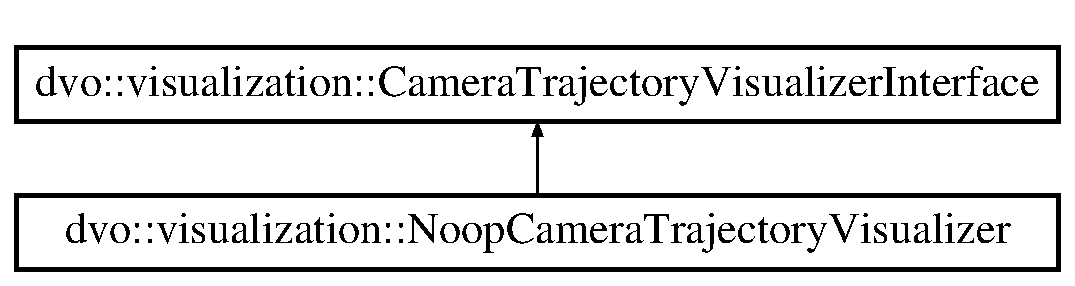
\includegraphics[height=2.000000cm]{classdvo_1_1visualization_1_1_noop_camera_trajectory_visualizer}
\end{center}
\end{figure}
\subsection*{Public Member Functions}
\begin{DoxyCompactItemize}
\item 
\mbox{\hyperlink{classdvo_1_1visualization_1_1_noop_camera_trajectory_visualizer_a3ef47107df86a08263381af353a70017}{Noop\+Camera\+Trajectory\+Visualizer}} ()
\item 
virtual \mbox{\hyperlink{classdvo_1_1visualization_1_1_noop_camera_trajectory_visualizer_a95788f9067a0da57c0da26c72be8143a}{$\sim$\+Noop\+Camera\+Trajectory\+Visualizer}} ()
\item 
virtual \mbox{\hyperlink{classdvo_1_1visualization_1_1_camera_visualizer_a473ebecc62e1d4edba21027d858789a2}{Camera\+Visualizer\+::\+Ptr}} \mbox{\hyperlink{classdvo_1_1visualization_1_1_noop_camera_trajectory_visualizer_afaf7c129a6112015c81a2e25d0002966}{camera}} (std\+::string name)
\item 
virtual \mbox{\hyperlink{classdvo_1_1visualization_1_1_trajectory_visualizer_aac33ef5979fe64ee33409f1afa977fd3}{Trajectory\+Visualizer\+::\+Ptr}} \mbox{\hyperlink{classdvo_1_1visualization_1_1_noop_camera_trajectory_visualizer_a73cd3c7ed8a3817c5f6d480d97aa24c5}{trajectory}} (std\+::string name)
\item 
virtual void \mbox{\hyperlink{classdvo_1_1visualization_1_1_noop_camera_trajectory_visualizer_afa3b5e4aff0306755ca3b53ef70008c4}{reset}} ()
\end{DoxyCompactItemize}


\subsection{Constructor \& Destructor Documentation}
\mbox{\Hypertarget{classdvo_1_1visualization_1_1_noop_camera_trajectory_visualizer_a3ef47107df86a08263381af353a70017}\label{classdvo_1_1visualization_1_1_noop_camera_trajectory_visualizer_a3ef47107df86a08263381af353a70017}} 
\index{dvo\+::visualization\+::\+Noop\+Camera\+Trajectory\+Visualizer@{dvo\+::visualization\+::\+Noop\+Camera\+Trajectory\+Visualizer}!Noop\+Camera\+Trajectory\+Visualizer@{Noop\+Camera\+Trajectory\+Visualizer}}
\index{Noop\+Camera\+Trajectory\+Visualizer@{Noop\+Camera\+Trajectory\+Visualizer}!dvo\+::visualization\+::\+Noop\+Camera\+Trajectory\+Visualizer@{dvo\+::visualization\+::\+Noop\+Camera\+Trajectory\+Visualizer}}
\subsubsection{\texorpdfstring{Noop\+Camera\+Trajectory\+Visualizer()}{NoopCameraTrajectoryVisualizer()}}
{\footnotesize\ttfamily dvo\+::visualization\+::\+Noop\+Camera\+Trajectory\+Visualizer\+::\+Noop\+Camera\+Trajectory\+Visualizer (\begin{DoxyParamCaption}{ }\end{DoxyParamCaption})}

\mbox{\Hypertarget{classdvo_1_1visualization_1_1_noop_camera_trajectory_visualizer_a95788f9067a0da57c0da26c72be8143a}\label{classdvo_1_1visualization_1_1_noop_camera_trajectory_visualizer_a95788f9067a0da57c0da26c72be8143a}} 
\index{dvo\+::visualization\+::\+Noop\+Camera\+Trajectory\+Visualizer@{dvo\+::visualization\+::\+Noop\+Camera\+Trajectory\+Visualizer}!````~Noop\+Camera\+Trajectory\+Visualizer@{$\sim$\+Noop\+Camera\+Trajectory\+Visualizer}}
\index{````~Noop\+Camera\+Trajectory\+Visualizer@{$\sim$\+Noop\+Camera\+Trajectory\+Visualizer}!dvo\+::visualization\+::\+Noop\+Camera\+Trajectory\+Visualizer@{dvo\+::visualization\+::\+Noop\+Camera\+Trajectory\+Visualizer}}
\subsubsection{\texorpdfstring{$\sim$\+Noop\+Camera\+Trajectory\+Visualizer()}{~NoopCameraTrajectoryVisualizer()}}
{\footnotesize\ttfamily dvo\+::visualization\+::\+Noop\+Camera\+Trajectory\+Visualizer\+::$\sim$\+Noop\+Camera\+Trajectory\+Visualizer (\begin{DoxyParamCaption}{ }\end{DoxyParamCaption})\hspace{0.3cm}{\ttfamily [virtual]}}



\subsection{Member Function Documentation}
\mbox{\Hypertarget{classdvo_1_1visualization_1_1_noop_camera_trajectory_visualizer_afaf7c129a6112015c81a2e25d0002966}\label{classdvo_1_1visualization_1_1_noop_camera_trajectory_visualizer_afaf7c129a6112015c81a2e25d0002966}} 
\index{dvo\+::visualization\+::\+Noop\+Camera\+Trajectory\+Visualizer@{dvo\+::visualization\+::\+Noop\+Camera\+Trajectory\+Visualizer}!camera@{camera}}
\index{camera@{camera}!dvo\+::visualization\+::\+Noop\+Camera\+Trajectory\+Visualizer@{dvo\+::visualization\+::\+Noop\+Camera\+Trajectory\+Visualizer}}
\subsubsection{\texorpdfstring{camera()}{camera()}}
{\footnotesize\ttfamily \mbox{\hyperlink{classdvo_1_1visualization_1_1_camera_visualizer_a473ebecc62e1d4edba21027d858789a2}{Camera\+Visualizer\+::\+Ptr}} dvo\+::visualization\+::\+Noop\+Camera\+Trajectory\+Visualizer\+::camera (\begin{DoxyParamCaption}\item[{std\+::string}]{name }\end{DoxyParamCaption})\hspace{0.3cm}{\ttfamily [virtual]}}



Implements \mbox{\hyperlink{classdvo_1_1visualization_1_1_camera_trajectory_visualizer_interface_a4d43cd43f26bd880eb07e8ee37a7154a}{dvo\+::visualization\+::\+Camera\+Trajectory\+Visualizer\+Interface}}.

\mbox{\Hypertarget{classdvo_1_1visualization_1_1_noop_camera_trajectory_visualizer_afa3b5e4aff0306755ca3b53ef70008c4}\label{classdvo_1_1visualization_1_1_noop_camera_trajectory_visualizer_afa3b5e4aff0306755ca3b53ef70008c4}} 
\index{dvo\+::visualization\+::\+Noop\+Camera\+Trajectory\+Visualizer@{dvo\+::visualization\+::\+Noop\+Camera\+Trajectory\+Visualizer}!reset@{reset}}
\index{reset@{reset}!dvo\+::visualization\+::\+Noop\+Camera\+Trajectory\+Visualizer@{dvo\+::visualization\+::\+Noop\+Camera\+Trajectory\+Visualizer}}
\subsubsection{\texorpdfstring{reset()}{reset()}}
{\footnotesize\ttfamily void dvo\+::visualization\+::\+Noop\+Camera\+Trajectory\+Visualizer\+::reset (\begin{DoxyParamCaption}{ }\end{DoxyParamCaption})\hspace{0.3cm}{\ttfamily [virtual]}}



Implements \mbox{\hyperlink{classdvo_1_1visualization_1_1_camera_trajectory_visualizer_interface_abcc7ddffc30b41eb9112c386f3e41aa7}{dvo\+::visualization\+::\+Camera\+Trajectory\+Visualizer\+Interface}}.

\mbox{\Hypertarget{classdvo_1_1visualization_1_1_noop_camera_trajectory_visualizer_a73cd3c7ed8a3817c5f6d480d97aa24c5}\label{classdvo_1_1visualization_1_1_noop_camera_trajectory_visualizer_a73cd3c7ed8a3817c5f6d480d97aa24c5}} 
\index{dvo\+::visualization\+::\+Noop\+Camera\+Trajectory\+Visualizer@{dvo\+::visualization\+::\+Noop\+Camera\+Trajectory\+Visualizer}!trajectory@{trajectory}}
\index{trajectory@{trajectory}!dvo\+::visualization\+::\+Noop\+Camera\+Trajectory\+Visualizer@{dvo\+::visualization\+::\+Noop\+Camera\+Trajectory\+Visualizer}}
\subsubsection{\texorpdfstring{trajectory()}{trajectory()}}
{\footnotesize\ttfamily \mbox{\hyperlink{classdvo_1_1visualization_1_1_trajectory_visualizer_aac33ef5979fe64ee33409f1afa977fd3}{Trajectory\+Visualizer\+::\+Ptr}} dvo\+::visualization\+::\+Noop\+Camera\+Trajectory\+Visualizer\+::trajectory (\begin{DoxyParamCaption}\item[{std\+::string}]{name }\end{DoxyParamCaption})\hspace{0.3cm}{\ttfamily [virtual]}}



Implements \mbox{\hyperlink{classdvo_1_1visualization_1_1_camera_trajectory_visualizer_interface_ac658e841335e51c50325267de10e64b3}{dvo\+::visualization\+::\+Camera\+Trajectory\+Visualizer\+Interface}}.



The documentation for this class was generated from the following files\+:\begin{DoxyCompactItemize}
\item 
dvo\+\_\+core/include/dvo/visualization/\mbox{\hyperlink{camera__trajectory__visualizer_8h}{camera\+\_\+trajectory\+\_\+visualizer.\+h}}\item 
dvo\+\_\+core/src/visualization/\mbox{\hyperlink{camera__trajectory__visualizer_8cpp}{camera\+\_\+trajectory\+\_\+visualizer.\+cpp}}\end{DoxyCompactItemize}

\hypertarget{classdvo_1_1visualization_1_1_noop_camera_visualizer}{}\section{dvo\+:\+:visualization\+:\+:Noop\+Camera\+Visualizer Class Reference}
\label{classdvo_1_1visualization_1_1_noop_camera_visualizer}\index{dvo\+::visualization\+::\+Noop\+Camera\+Visualizer@{dvo\+::visualization\+::\+Noop\+Camera\+Visualizer}}
Inheritance diagram for dvo\+:\+:visualization\+:\+:Noop\+Camera\+Visualizer\+:\begin{figure}[H]
\begin{center}
\leavevmode
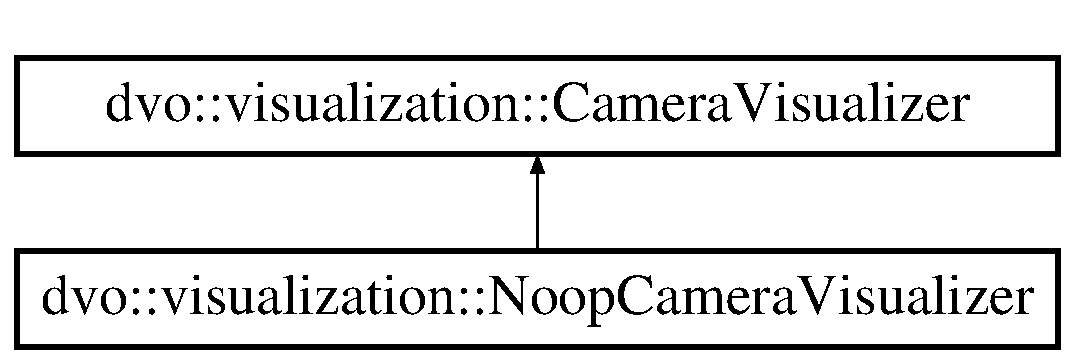
\includegraphics[height=2.000000cm]{classdvo_1_1visualization_1_1_noop_camera_visualizer}
\end{center}
\end{figure}
\subsection*{Public Member Functions}
\begin{DoxyCompactItemize}
\item 
\mbox{\hyperlink{classdvo_1_1visualization_1_1_noop_camera_visualizer_ade3cb140e752ade11e25f0ad049958af}{Noop\+Camera\+Visualizer}} ()
\item 
virtual \mbox{\hyperlink{classdvo_1_1visualization_1_1_noop_camera_visualizer_ae29e589ff8c183b11c1d2ac8e6072447}{$\sim$\+Noop\+Camera\+Visualizer}} ()
\item 
virtual void \mbox{\hyperlink{classdvo_1_1visualization_1_1_noop_camera_visualizer_acfb97efacfcb9e3dd30444e34c7bfd9c}{show}} (\mbox{\hyperlink{classdvo_1_1visualization_1_1_camera_visualizer_a0526f50be9f298c4f7d1f91018d50af7}{Option}} option=\mbox{\hyperlink{classdvo_1_1visualization_1_1_camera_visualizer_a0526f50be9f298c4f7d1f91018d50af7a0ff8fc7d7283f27066e93ca0d4ef3f19}{Show\+Camera\+And\+Cloud}})
\item 
virtual void \mbox{\hyperlink{classdvo_1_1visualization_1_1_noop_camera_visualizer_a875ff591e3db513ddbec48478989639e}{hide}} ()
\item 
virtual \mbox{\hyperlink{classdvo_1_1visualization_1_1_camera_visualizer}{Camera\+Visualizer}} \& \mbox{\hyperlink{classdvo_1_1visualization_1_1_noop_camera_visualizer_a7983d8de9de45c5617c3e877d36d6ff3}{update}} (const \mbox{\hyperlink{structdvo_1_1core_1_1_rgbd_image}{dvo\+::core\+::\+Rgbd\+Image}} \&img, const \mbox{\hyperlink{structdvo_1_1core_1_1_intrinsic_matrix}{dvo\+::core\+::\+Intrinsic\+Matrix}} \&intrinsics, const Eigen\+::\+Affine3d \&pose)
\end{DoxyCompactItemize}
\subsection*{Additional Inherited Members}


\subsection{Constructor \& Destructor Documentation}
\mbox{\Hypertarget{classdvo_1_1visualization_1_1_noop_camera_visualizer_ade3cb140e752ade11e25f0ad049958af}\label{classdvo_1_1visualization_1_1_noop_camera_visualizer_ade3cb140e752ade11e25f0ad049958af}} 
\index{dvo\+::visualization\+::\+Noop\+Camera\+Visualizer@{dvo\+::visualization\+::\+Noop\+Camera\+Visualizer}!Noop\+Camera\+Visualizer@{Noop\+Camera\+Visualizer}}
\index{Noop\+Camera\+Visualizer@{Noop\+Camera\+Visualizer}!dvo\+::visualization\+::\+Noop\+Camera\+Visualizer@{dvo\+::visualization\+::\+Noop\+Camera\+Visualizer}}
\subsubsection{\texorpdfstring{Noop\+Camera\+Visualizer()}{NoopCameraVisualizer()}}
{\footnotesize\ttfamily dvo\+::visualization\+::\+Noop\+Camera\+Visualizer\+::\+Noop\+Camera\+Visualizer (\begin{DoxyParamCaption}{ }\end{DoxyParamCaption})\hspace{0.3cm}{\ttfamily [inline]}}

\mbox{\Hypertarget{classdvo_1_1visualization_1_1_noop_camera_visualizer_ae29e589ff8c183b11c1d2ac8e6072447}\label{classdvo_1_1visualization_1_1_noop_camera_visualizer_ae29e589ff8c183b11c1d2ac8e6072447}} 
\index{dvo\+::visualization\+::\+Noop\+Camera\+Visualizer@{dvo\+::visualization\+::\+Noop\+Camera\+Visualizer}!````~Noop\+Camera\+Visualizer@{$\sim$\+Noop\+Camera\+Visualizer}}
\index{````~Noop\+Camera\+Visualizer@{$\sim$\+Noop\+Camera\+Visualizer}!dvo\+::visualization\+::\+Noop\+Camera\+Visualizer@{dvo\+::visualization\+::\+Noop\+Camera\+Visualizer}}
\subsubsection{\texorpdfstring{$\sim$\+Noop\+Camera\+Visualizer()}{~NoopCameraVisualizer()}}
{\footnotesize\ttfamily virtual dvo\+::visualization\+::\+Noop\+Camera\+Visualizer\+::$\sim$\+Noop\+Camera\+Visualizer (\begin{DoxyParamCaption}{ }\end{DoxyParamCaption})\hspace{0.3cm}{\ttfamily [inline]}, {\ttfamily [virtual]}}



\subsection{Member Function Documentation}
\mbox{\Hypertarget{classdvo_1_1visualization_1_1_noop_camera_visualizer_a875ff591e3db513ddbec48478989639e}\label{classdvo_1_1visualization_1_1_noop_camera_visualizer_a875ff591e3db513ddbec48478989639e}} 
\index{dvo\+::visualization\+::\+Noop\+Camera\+Visualizer@{dvo\+::visualization\+::\+Noop\+Camera\+Visualizer}!hide@{hide}}
\index{hide@{hide}!dvo\+::visualization\+::\+Noop\+Camera\+Visualizer@{dvo\+::visualization\+::\+Noop\+Camera\+Visualizer}}
\subsubsection{\texorpdfstring{hide()}{hide()}}
{\footnotesize\ttfamily virtual void dvo\+::visualization\+::\+Noop\+Camera\+Visualizer\+::hide (\begin{DoxyParamCaption}{ }\end{DoxyParamCaption})\hspace{0.3cm}{\ttfamily [inline]}, {\ttfamily [virtual]}}



Implements \mbox{\hyperlink{classdvo_1_1visualization_1_1_camera_visualizer_a45dbf0d449a7b7529f7da477c676ca85}{dvo\+::visualization\+::\+Camera\+Visualizer}}.

\mbox{\Hypertarget{classdvo_1_1visualization_1_1_noop_camera_visualizer_acfb97efacfcb9e3dd30444e34c7bfd9c}\label{classdvo_1_1visualization_1_1_noop_camera_visualizer_acfb97efacfcb9e3dd30444e34c7bfd9c}} 
\index{dvo\+::visualization\+::\+Noop\+Camera\+Visualizer@{dvo\+::visualization\+::\+Noop\+Camera\+Visualizer}!show@{show}}
\index{show@{show}!dvo\+::visualization\+::\+Noop\+Camera\+Visualizer@{dvo\+::visualization\+::\+Noop\+Camera\+Visualizer}}
\subsubsection{\texorpdfstring{show()}{show()}}
{\footnotesize\ttfamily virtual void dvo\+::visualization\+::\+Noop\+Camera\+Visualizer\+::show (\begin{DoxyParamCaption}\item[{\mbox{\hyperlink{classdvo_1_1visualization_1_1_camera_visualizer_a0526f50be9f298c4f7d1f91018d50af7}{Option}}}]{option = {\ttfamily \mbox{\hyperlink{classdvo_1_1visualization_1_1_camera_visualizer_a0526f50be9f298c4f7d1f91018d50af7a0ff8fc7d7283f27066e93ca0d4ef3f19}{Show\+Camera\+And\+Cloud}}} }\end{DoxyParamCaption})\hspace{0.3cm}{\ttfamily [inline]}, {\ttfamily [virtual]}}



Implements \mbox{\hyperlink{classdvo_1_1visualization_1_1_camera_visualizer_a646b21ea800d07f6a4174c80daf2bf50}{dvo\+::visualization\+::\+Camera\+Visualizer}}.

\mbox{\Hypertarget{classdvo_1_1visualization_1_1_noop_camera_visualizer_a7983d8de9de45c5617c3e877d36d6ff3}\label{classdvo_1_1visualization_1_1_noop_camera_visualizer_a7983d8de9de45c5617c3e877d36d6ff3}} 
\index{dvo\+::visualization\+::\+Noop\+Camera\+Visualizer@{dvo\+::visualization\+::\+Noop\+Camera\+Visualizer}!update@{update}}
\index{update@{update}!dvo\+::visualization\+::\+Noop\+Camera\+Visualizer@{dvo\+::visualization\+::\+Noop\+Camera\+Visualizer}}
\subsubsection{\texorpdfstring{update()}{update()}}
{\footnotesize\ttfamily virtual \mbox{\hyperlink{classdvo_1_1visualization_1_1_camera_visualizer}{Camera\+Visualizer}}\& dvo\+::visualization\+::\+Noop\+Camera\+Visualizer\+::update (\begin{DoxyParamCaption}\item[{const \mbox{\hyperlink{structdvo_1_1core_1_1_rgbd_image}{dvo\+::core\+::\+Rgbd\+Image}} \&}]{img,  }\item[{const \mbox{\hyperlink{structdvo_1_1core_1_1_intrinsic_matrix}{dvo\+::core\+::\+Intrinsic\+Matrix}} \&}]{intrinsics,  }\item[{const Eigen\+::\+Affine3d \&}]{pose }\end{DoxyParamCaption})\hspace{0.3cm}{\ttfamily [inline]}, {\ttfamily [virtual]}}



Implements \mbox{\hyperlink{classdvo_1_1visualization_1_1_camera_visualizer_afd83119e63048b0229820045d54c95ec}{dvo\+::visualization\+::\+Camera\+Visualizer}}.



The documentation for this class was generated from the following file\+:\begin{DoxyCompactItemize}
\item 
dvo\+\_\+core/src/visualization/\mbox{\hyperlink{camera__trajectory__visualizer_8cpp}{camera\+\_\+trajectory\+\_\+visualizer.\+cpp}}\end{DoxyCompactItemize}

\hypertarget{classdvo_1_1visualization_1_1_noop_trajectory_visualizer}{}\section{dvo\+:\+:visualization\+:\+:Noop\+Trajectory\+Visualizer Class Reference}
\label{classdvo_1_1visualization_1_1_noop_trajectory_visualizer}\index{dvo\+::visualization\+::\+Noop\+Trajectory\+Visualizer@{dvo\+::visualization\+::\+Noop\+Trajectory\+Visualizer}}
Inheritance diagram for dvo\+:\+:visualization\+:\+:Noop\+Trajectory\+Visualizer\+:\begin{figure}[H]
\begin{center}
\leavevmode
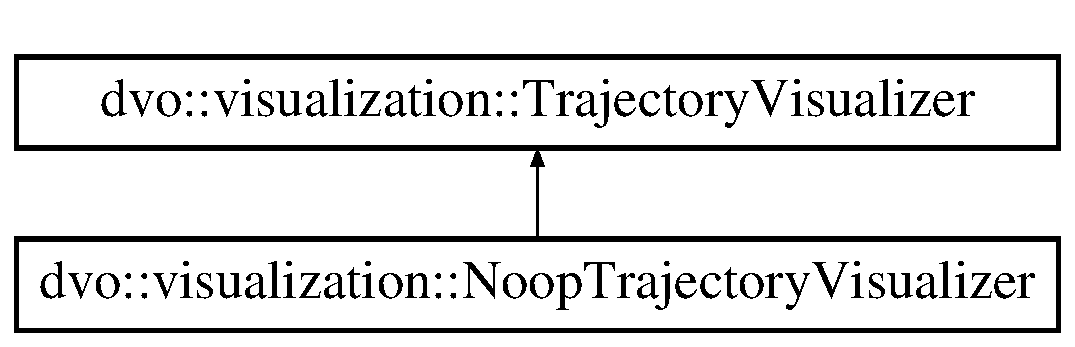
\includegraphics[height=2.000000cm]{classdvo_1_1visualization_1_1_noop_trajectory_visualizer}
\end{center}
\end{figure}
\subsection*{Public Member Functions}
\begin{DoxyCompactItemize}
\item 
\mbox{\hyperlink{classdvo_1_1visualization_1_1_noop_trajectory_visualizer_a215b180a6d70948c2448ed7d0edc0852}{Noop\+Trajectory\+Visualizer}} ()
\item 
virtual \mbox{\hyperlink{classdvo_1_1visualization_1_1_noop_trajectory_visualizer_a2f3efe6c4bb5b294c72c594ef13060ca}{$\sim$\+Noop\+Trajectory\+Visualizer}} ()
\item 
virtual \mbox{\hyperlink{classdvo_1_1visualization_1_1_trajectory_visualizer}{Trajectory\+Visualizer}} \& \mbox{\hyperlink{classdvo_1_1visualization_1_1_noop_trajectory_visualizer_a40e9cfd01744c3efa85afb93237e2030}{add}} (const Eigen\+::\+Affine3d \&pose)
\end{DoxyCompactItemize}
\subsection*{Additional Inherited Members}


\subsection{Constructor \& Destructor Documentation}
\mbox{\Hypertarget{classdvo_1_1visualization_1_1_noop_trajectory_visualizer_a215b180a6d70948c2448ed7d0edc0852}\label{classdvo_1_1visualization_1_1_noop_trajectory_visualizer_a215b180a6d70948c2448ed7d0edc0852}} 
\index{dvo\+::visualization\+::\+Noop\+Trajectory\+Visualizer@{dvo\+::visualization\+::\+Noop\+Trajectory\+Visualizer}!Noop\+Trajectory\+Visualizer@{Noop\+Trajectory\+Visualizer}}
\index{Noop\+Trajectory\+Visualizer@{Noop\+Trajectory\+Visualizer}!dvo\+::visualization\+::\+Noop\+Trajectory\+Visualizer@{dvo\+::visualization\+::\+Noop\+Trajectory\+Visualizer}}
\subsubsection{\texorpdfstring{Noop\+Trajectory\+Visualizer()}{NoopTrajectoryVisualizer()}}
{\footnotesize\ttfamily dvo\+::visualization\+::\+Noop\+Trajectory\+Visualizer\+::\+Noop\+Trajectory\+Visualizer (\begin{DoxyParamCaption}{ }\end{DoxyParamCaption})\hspace{0.3cm}{\ttfamily [inline]}}

\mbox{\Hypertarget{classdvo_1_1visualization_1_1_noop_trajectory_visualizer_a2f3efe6c4bb5b294c72c594ef13060ca}\label{classdvo_1_1visualization_1_1_noop_trajectory_visualizer_a2f3efe6c4bb5b294c72c594ef13060ca}} 
\index{dvo\+::visualization\+::\+Noop\+Trajectory\+Visualizer@{dvo\+::visualization\+::\+Noop\+Trajectory\+Visualizer}!````~Noop\+Trajectory\+Visualizer@{$\sim$\+Noop\+Trajectory\+Visualizer}}
\index{````~Noop\+Trajectory\+Visualizer@{$\sim$\+Noop\+Trajectory\+Visualizer}!dvo\+::visualization\+::\+Noop\+Trajectory\+Visualizer@{dvo\+::visualization\+::\+Noop\+Trajectory\+Visualizer}}
\subsubsection{\texorpdfstring{$\sim$\+Noop\+Trajectory\+Visualizer()}{~NoopTrajectoryVisualizer()}}
{\footnotesize\ttfamily virtual dvo\+::visualization\+::\+Noop\+Trajectory\+Visualizer\+::$\sim$\+Noop\+Trajectory\+Visualizer (\begin{DoxyParamCaption}{ }\end{DoxyParamCaption})\hspace{0.3cm}{\ttfamily [inline]}, {\ttfamily [virtual]}}



\subsection{Member Function Documentation}
\mbox{\Hypertarget{classdvo_1_1visualization_1_1_noop_trajectory_visualizer_a40e9cfd01744c3efa85afb93237e2030}\label{classdvo_1_1visualization_1_1_noop_trajectory_visualizer_a40e9cfd01744c3efa85afb93237e2030}} 
\index{dvo\+::visualization\+::\+Noop\+Trajectory\+Visualizer@{dvo\+::visualization\+::\+Noop\+Trajectory\+Visualizer}!add@{add}}
\index{add@{add}!dvo\+::visualization\+::\+Noop\+Trajectory\+Visualizer@{dvo\+::visualization\+::\+Noop\+Trajectory\+Visualizer}}
\subsubsection{\texorpdfstring{add()}{add()}}
{\footnotesize\ttfamily virtual \mbox{\hyperlink{classdvo_1_1visualization_1_1_trajectory_visualizer}{Trajectory\+Visualizer}}\& dvo\+::visualization\+::\+Noop\+Trajectory\+Visualizer\+::add (\begin{DoxyParamCaption}\item[{const Eigen\+::\+Affine3d \&}]{pose }\end{DoxyParamCaption})\hspace{0.3cm}{\ttfamily [inline]}, {\ttfamily [virtual]}}



Implements \mbox{\hyperlink{classdvo_1_1visualization_1_1_trajectory_visualizer_ac41106ae7e28c019b03f0aa210c6f0c1}{dvo\+::visualization\+::\+Trajectory\+Visualizer}}.



The documentation for this class was generated from the following file\+:\begin{DoxyCompactItemize}
\item 
dvo\+\_\+core/src/visualization/\mbox{\hyperlink{camera__trajectory__visualizer_8cpp}{camera\+\_\+trajectory\+\_\+visualizer.\+cpp}}\end{DoxyCompactItemize}

\hypertarget{classdvo_1_1core_1_1_normal_distribution_scale_estimator}{}\section{dvo\+:\+:core\+:\+:Normal\+Distribution\+Scale\+Estimator Class Reference}
\label{classdvo_1_1core_1_1_normal_distribution_scale_estimator}\index{dvo\+::core\+::\+Normal\+Distribution\+Scale\+Estimator@{dvo\+::core\+::\+Normal\+Distribution\+Scale\+Estimator}}


{\ttfamily \#include $<$weight\+\_\+calculation.\+h$>$}

Inheritance diagram for dvo\+:\+:core\+:\+:Normal\+Distribution\+Scale\+Estimator\+:\begin{figure}[H]
\begin{center}
\leavevmode
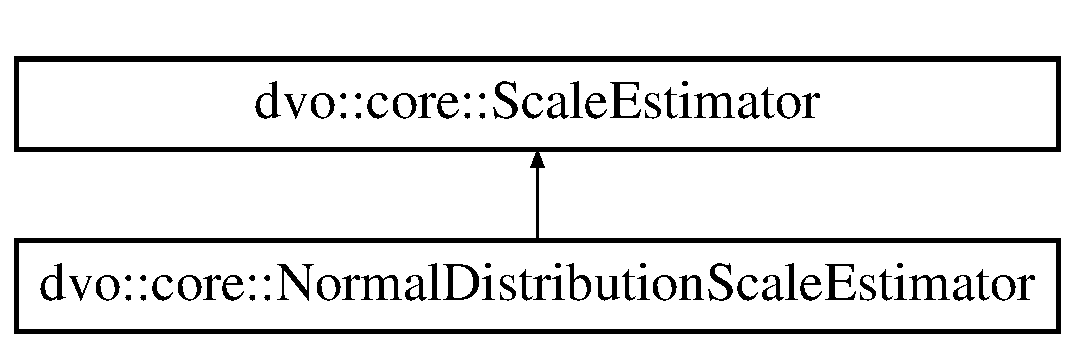
\includegraphics[height=2.000000cm]{classdvo_1_1core_1_1_normal_distribution_scale_estimator}
\end{center}
\end{figure}
\subsection*{Public Member Functions}
\begin{DoxyCompactItemize}
\item 
\mbox{\hyperlink{classdvo_1_1core_1_1_normal_distribution_scale_estimator_a22c312392df41e92c192e4c8372e07d0}{Normal\+Distribution\+Scale\+Estimator}} ()
\item 
virtual \mbox{\hyperlink{classdvo_1_1core_1_1_normal_distribution_scale_estimator_aaa1775b69e07b45786f317f71ae8fad2}{$\sim$\+Normal\+Distribution\+Scale\+Estimator}} ()
\item 
virtual float \mbox{\hyperlink{classdvo_1_1core_1_1_normal_distribution_scale_estimator_a0aa8db7144ffcd1d06704dbf89997446}{compute}} (const cv\+::\+Mat \&errors) const
\end{DoxyCompactItemize}


\subsection{Constructor \& Destructor Documentation}
\mbox{\Hypertarget{classdvo_1_1core_1_1_normal_distribution_scale_estimator_a22c312392df41e92c192e4c8372e07d0}\label{classdvo_1_1core_1_1_normal_distribution_scale_estimator_a22c312392df41e92c192e4c8372e07d0}} 
\index{dvo\+::core\+::\+Normal\+Distribution\+Scale\+Estimator@{dvo\+::core\+::\+Normal\+Distribution\+Scale\+Estimator}!Normal\+Distribution\+Scale\+Estimator@{Normal\+Distribution\+Scale\+Estimator}}
\index{Normal\+Distribution\+Scale\+Estimator@{Normal\+Distribution\+Scale\+Estimator}!dvo\+::core\+::\+Normal\+Distribution\+Scale\+Estimator@{dvo\+::core\+::\+Normal\+Distribution\+Scale\+Estimator}}
\subsubsection{\texorpdfstring{Normal\+Distribution\+Scale\+Estimator()}{NormalDistributionScaleEstimator()}}
{\footnotesize\ttfamily dvo\+::core\+::\+Normal\+Distribution\+Scale\+Estimator\+::\+Normal\+Distribution\+Scale\+Estimator (\begin{DoxyParamCaption}{ }\end{DoxyParamCaption})}

\mbox{\Hypertarget{classdvo_1_1core_1_1_normal_distribution_scale_estimator_aaa1775b69e07b45786f317f71ae8fad2}\label{classdvo_1_1core_1_1_normal_distribution_scale_estimator_aaa1775b69e07b45786f317f71ae8fad2}} 
\index{dvo\+::core\+::\+Normal\+Distribution\+Scale\+Estimator@{dvo\+::core\+::\+Normal\+Distribution\+Scale\+Estimator}!````~Normal\+Distribution\+Scale\+Estimator@{$\sim$\+Normal\+Distribution\+Scale\+Estimator}}
\index{````~Normal\+Distribution\+Scale\+Estimator@{$\sim$\+Normal\+Distribution\+Scale\+Estimator}!dvo\+::core\+::\+Normal\+Distribution\+Scale\+Estimator@{dvo\+::core\+::\+Normal\+Distribution\+Scale\+Estimator}}
\subsubsection{\texorpdfstring{$\sim$\+Normal\+Distribution\+Scale\+Estimator()}{~NormalDistributionScaleEstimator()}}
{\footnotesize\ttfamily virtual dvo\+::core\+::\+Normal\+Distribution\+Scale\+Estimator\+::$\sim$\+Normal\+Distribution\+Scale\+Estimator (\begin{DoxyParamCaption}{ }\end{DoxyParamCaption})\hspace{0.3cm}{\ttfamily [inline]}, {\ttfamily [virtual]}}



\subsection{Member Function Documentation}
\mbox{\Hypertarget{classdvo_1_1core_1_1_normal_distribution_scale_estimator_a0aa8db7144ffcd1d06704dbf89997446}\label{classdvo_1_1core_1_1_normal_distribution_scale_estimator_a0aa8db7144ffcd1d06704dbf89997446}} 
\index{dvo\+::core\+::\+Normal\+Distribution\+Scale\+Estimator@{dvo\+::core\+::\+Normal\+Distribution\+Scale\+Estimator}!compute@{compute}}
\index{compute@{compute}!dvo\+::core\+::\+Normal\+Distribution\+Scale\+Estimator@{dvo\+::core\+::\+Normal\+Distribution\+Scale\+Estimator}}
\subsubsection{\texorpdfstring{compute()}{compute()}}
{\footnotesize\ttfamily float dvo\+::core\+::\+Normal\+Distribution\+Scale\+Estimator\+::compute (\begin{DoxyParamCaption}\item[{const cv\+::\+Mat \&}]{errors }\end{DoxyParamCaption}) const\hspace{0.3cm}{\ttfamily [virtual]}}



Implements \mbox{\hyperlink{classdvo_1_1core_1_1_scale_estimator_a6968ac2cd37c2ce1c966f0c9e17d1a3c}{dvo\+::core\+::\+Scale\+Estimator}}.



The documentation for this class was generated from the following files\+:\begin{DoxyCompactItemize}
\item 
dvo\+\_\+core/include/dvo/core/\mbox{\hyperlink{weight__calculation_8h}{weight\+\_\+calculation.\+h}}\item 
dvo\+\_\+core/src/core/\mbox{\hyperlink{weight__calculation_8cpp}{weight\+\_\+calculation.\+cpp}}\end{DoxyCompactItemize}

\hypertarget{classdvo_1_1core_1_1_normal_equations_least_squares}{}\section{dvo\+:\+:core\+:\+:Normal\+Equations\+Least\+Squares Class Reference}
\label{classdvo_1_1core_1_1_normal_equations_least_squares}\index{dvo\+::core\+::\+Normal\+Equations\+Least\+Squares@{dvo\+::core\+::\+Normal\+Equations\+Least\+Squares}}


{\ttfamily \#include $<$least\+\_\+squares.\+h$>$}

Inheritance diagram for dvo\+:\+:core\+:\+:Normal\+Equations\+Least\+Squares\+:\begin{figure}[H]
\begin{center}
\leavevmode
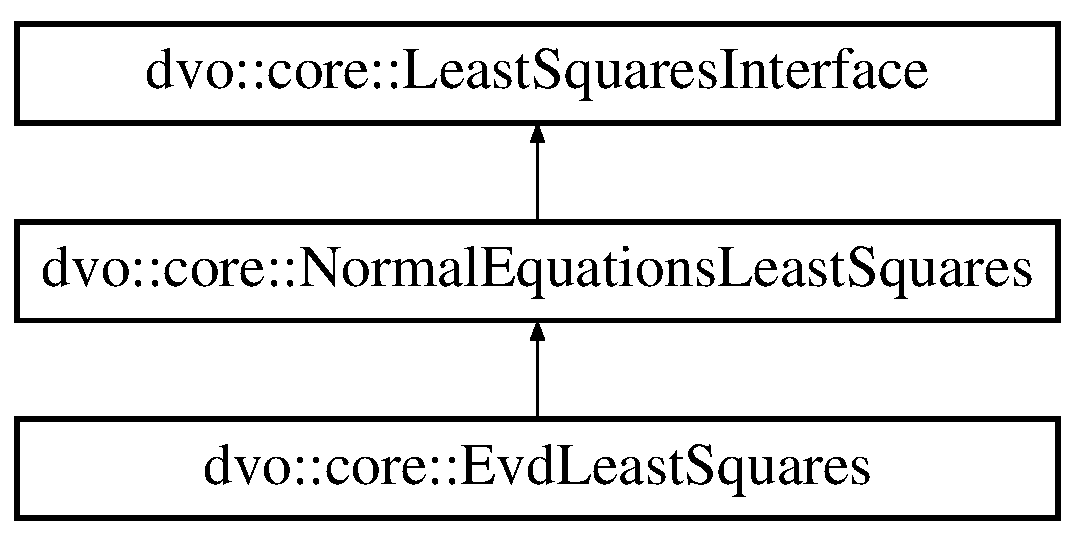
\includegraphics[height=3.000000cm]{classdvo_1_1core_1_1_normal_equations_least_squares}
\end{center}
\end{figure}
\subsection*{Public Member Functions}
\begin{DoxyCompactItemize}
\item 
virtual \mbox{\hyperlink{classdvo_1_1core_1_1_normal_equations_least_squares_a7507274ad0f440898f4eaa7c24874c81}{$\sim$\+Normal\+Equations\+Least\+Squares}} ()
\item 
virtual void \mbox{\hyperlink{classdvo_1_1core_1_1_normal_equations_least_squares_a4799d66e3dc176ab07418fc1cfacfb53}{initialize}} (const size\+\_\+t \mbox{\hyperlink{classdvo_1_1core_1_1_normal_equations_least_squares_a59cc5b0c4bc11f31fff1a4dfd5ad1fe7}{maxnum\+\_\+constraints}})
\item 
virtual void \mbox{\hyperlink{classdvo_1_1core_1_1_normal_equations_least_squares_a1ef767b22d889c99850b1b2dd8cd870d}{update}} (const \mbox{\hyperlink{namespacedvo_1_1core_a05327f3312d32a301bce9fccda9e5807}{Vector6}} \&J, const \mbox{\hyperlink{namespacedvo_1_1core_ab9c199d221775a923e2549ad7e15c323}{Num\+Type}} \&res, const \mbox{\hyperlink{namespacedvo_1_1core_ab9c199d221775a923e2549ad7e15c323}{Num\+Type}} \&weight=1.\+0f)
\item 
virtual void \mbox{\hyperlink{classdvo_1_1core_1_1_normal_equations_least_squares_a0da5301414f684b8e3ebfa9c4794af31}{finish}} ()
\item 
virtual void \mbox{\hyperlink{classdvo_1_1core_1_1_normal_equations_least_squares_a8a25d3970f6506df2066995f2f2effda}{solve}} (\mbox{\hyperlink{namespacedvo_1_1core_a05327f3312d32a301bce9fccda9e5807}{Vector6}} \&x)
\item 
void \mbox{\hyperlink{classdvo_1_1core_1_1_normal_equations_least_squares_a9665b0bf93aac4348dc9ad18c39cf886}{combine}} (const \mbox{\hyperlink{classdvo_1_1core_1_1_normal_equations_least_squares}{Normal\+Equations\+Least\+Squares}} \&other)
\end{DoxyCompactItemize}
\subsection*{Public Attributes}
\begin{DoxyCompactItemize}
\item 
\mbox{\hyperlink{classdvo_1_1core_1_1_normal_equations_least_squares_a6bb9257ce532f01e50ad11ac525313be}{E\+I\+G\+E\+N\+\_\+\+M\+A\+K\+E\+\_\+\+A\+L\+I\+G\+N\+E\+D\+\_\+\+O\+P\+E\+R\+A\+T\+O\+R\+\_\+\+N\+EW}}
\item 
\mbox{\hyperlink{classdvo_1_1core_1_1_optimized_self_adjoint_matrix6x6f}{Optimized\+Self\+Adjoint\+Matrix6x6f}} \mbox{\hyperlink{classdvo_1_1core_1_1_normal_equations_least_squares_aac97b94e748b2ded6104bd3edf52a8c6}{A\+\_\+opt}}
\item 
\mbox{\hyperlink{namespacedvo_1_1core_a7b76cdc563f01ec2220fd58316004626}{Matrix6x6}} \mbox{\hyperlink{classdvo_1_1core_1_1_normal_equations_least_squares_af47004a3887290742e297bc32320e98b}{A}}
\item 
\mbox{\hyperlink{namespacedvo_1_1core_a05327f3312d32a301bce9fccda9e5807}{Vector6}} \mbox{\hyperlink{classdvo_1_1core_1_1_normal_equations_least_squares_a055ee4893239c51a297340166aa4a8f4}{b}}
\item 
double \mbox{\hyperlink{classdvo_1_1core_1_1_normal_equations_least_squares_a8e147296081ecdbe25038b496d4c2130}{error}}
\item 
size\+\_\+t \mbox{\hyperlink{classdvo_1_1core_1_1_normal_equations_least_squares_a59cc5b0c4bc11f31fff1a4dfd5ad1fe7}{maxnum\+\_\+constraints}}
\item 
size\+\_\+t \mbox{\hyperlink{classdvo_1_1core_1_1_normal_equations_least_squares_a3e2e4db46014f3eefa3576b86278c9e0}{num\+\_\+constraints}}
\end{DoxyCompactItemize}


\subsection{Detailed Description}
Builds normal equations and solves them with Cholesky decomposition. 

\subsection{Constructor \& Destructor Documentation}
\mbox{\Hypertarget{classdvo_1_1core_1_1_normal_equations_least_squares_a7507274ad0f440898f4eaa7c24874c81}\label{classdvo_1_1core_1_1_normal_equations_least_squares_a7507274ad0f440898f4eaa7c24874c81}} 
\index{dvo\+::core\+::\+Normal\+Equations\+Least\+Squares@{dvo\+::core\+::\+Normal\+Equations\+Least\+Squares}!````~Normal\+Equations\+Least\+Squares@{$\sim$\+Normal\+Equations\+Least\+Squares}}
\index{````~Normal\+Equations\+Least\+Squares@{$\sim$\+Normal\+Equations\+Least\+Squares}!dvo\+::core\+::\+Normal\+Equations\+Least\+Squares@{dvo\+::core\+::\+Normal\+Equations\+Least\+Squares}}
\subsubsection{\texorpdfstring{$\sim$\+Normal\+Equations\+Least\+Squares()}{~NormalEquationsLeastSquares()}}
{\footnotesize\ttfamily dvo\+::core\+::\+Normal\+Equations\+Least\+Squares\+::$\sim$\+Normal\+Equations\+Least\+Squares (\begin{DoxyParamCaption}{ }\end{DoxyParamCaption})\hspace{0.3cm}{\ttfamily [virtual]}}



\subsection{Member Function Documentation}
\mbox{\Hypertarget{classdvo_1_1core_1_1_normal_equations_least_squares_a9665b0bf93aac4348dc9ad18c39cf886}\label{classdvo_1_1core_1_1_normal_equations_least_squares_a9665b0bf93aac4348dc9ad18c39cf886}} 
\index{dvo\+::core\+::\+Normal\+Equations\+Least\+Squares@{dvo\+::core\+::\+Normal\+Equations\+Least\+Squares}!combine@{combine}}
\index{combine@{combine}!dvo\+::core\+::\+Normal\+Equations\+Least\+Squares@{dvo\+::core\+::\+Normal\+Equations\+Least\+Squares}}
\subsubsection{\texorpdfstring{combine()}{combine()}}
{\footnotesize\ttfamily void dvo\+::core\+::\+Normal\+Equations\+Least\+Squares\+::combine (\begin{DoxyParamCaption}\item[{const \mbox{\hyperlink{classdvo_1_1core_1_1_normal_equations_least_squares}{Normal\+Equations\+Least\+Squares}} \&}]{other }\end{DoxyParamCaption})}

\mbox{\Hypertarget{classdvo_1_1core_1_1_normal_equations_least_squares_a0da5301414f684b8e3ebfa9c4794af31}\label{classdvo_1_1core_1_1_normal_equations_least_squares_a0da5301414f684b8e3ebfa9c4794af31}} 
\index{dvo\+::core\+::\+Normal\+Equations\+Least\+Squares@{dvo\+::core\+::\+Normal\+Equations\+Least\+Squares}!finish@{finish}}
\index{finish@{finish}!dvo\+::core\+::\+Normal\+Equations\+Least\+Squares@{dvo\+::core\+::\+Normal\+Equations\+Least\+Squares}}
\subsubsection{\texorpdfstring{finish()}{finish()}}
{\footnotesize\ttfamily void dvo\+::core\+::\+Normal\+Equations\+Least\+Squares\+::finish (\begin{DoxyParamCaption}{ }\end{DoxyParamCaption})\hspace{0.3cm}{\ttfamily [virtual]}}



Implements \mbox{\hyperlink{classdvo_1_1core_1_1_least_squares_interface_a2e580a70e96f0e7d6d70f6047891a42a}{dvo\+::core\+::\+Least\+Squares\+Interface}}.

\mbox{\Hypertarget{classdvo_1_1core_1_1_normal_equations_least_squares_a4799d66e3dc176ab07418fc1cfacfb53}\label{classdvo_1_1core_1_1_normal_equations_least_squares_a4799d66e3dc176ab07418fc1cfacfb53}} 
\index{dvo\+::core\+::\+Normal\+Equations\+Least\+Squares@{dvo\+::core\+::\+Normal\+Equations\+Least\+Squares}!initialize@{initialize}}
\index{initialize@{initialize}!dvo\+::core\+::\+Normal\+Equations\+Least\+Squares@{dvo\+::core\+::\+Normal\+Equations\+Least\+Squares}}
\subsubsection{\texorpdfstring{initialize()}{initialize()}}
{\footnotesize\ttfamily void dvo\+::core\+::\+Normal\+Equations\+Least\+Squares\+::initialize (\begin{DoxyParamCaption}\item[{const size\+\_\+t}]{maxnum\+\_\+constraints }\end{DoxyParamCaption})\hspace{0.3cm}{\ttfamily [virtual]}}



Implements \mbox{\hyperlink{classdvo_1_1core_1_1_least_squares_interface_a09e5784f74d7352a9550a8aa523d30d7}{dvo\+::core\+::\+Least\+Squares\+Interface}}.

\mbox{\Hypertarget{classdvo_1_1core_1_1_normal_equations_least_squares_a8a25d3970f6506df2066995f2f2effda}\label{classdvo_1_1core_1_1_normal_equations_least_squares_a8a25d3970f6506df2066995f2f2effda}} 
\index{dvo\+::core\+::\+Normal\+Equations\+Least\+Squares@{dvo\+::core\+::\+Normal\+Equations\+Least\+Squares}!solve@{solve}}
\index{solve@{solve}!dvo\+::core\+::\+Normal\+Equations\+Least\+Squares@{dvo\+::core\+::\+Normal\+Equations\+Least\+Squares}}
\subsubsection{\texorpdfstring{solve()}{solve()}}
{\footnotesize\ttfamily void dvo\+::core\+::\+Normal\+Equations\+Least\+Squares\+::solve (\begin{DoxyParamCaption}\item[{\mbox{\hyperlink{namespacedvo_1_1core_a05327f3312d32a301bce9fccda9e5807}{Vector6}} \&}]{x }\end{DoxyParamCaption})\hspace{0.3cm}{\ttfamily [virtual]}}



Implements \mbox{\hyperlink{classdvo_1_1core_1_1_least_squares_interface_a3e2b3c894c5286fdee79316e6fa4d691}{dvo\+::core\+::\+Least\+Squares\+Interface}}.



Reimplemented in \mbox{\hyperlink{classdvo_1_1core_1_1_evd_least_squares_a7264139b3006d803039707c4318d2451}{dvo\+::core\+::\+Evd\+Least\+Squares}}.

\mbox{\Hypertarget{classdvo_1_1core_1_1_normal_equations_least_squares_a1ef767b22d889c99850b1b2dd8cd870d}\label{classdvo_1_1core_1_1_normal_equations_least_squares_a1ef767b22d889c99850b1b2dd8cd870d}} 
\index{dvo\+::core\+::\+Normal\+Equations\+Least\+Squares@{dvo\+::core\+::\+Normal\+Equations\+Least\+Squares}!update@{update}}
\index{update@{update}!dvo\+::core\+::\+Normal\+Equations\+Least\+Squares@{dvo\+::core\+::\+Normal\+Equations\+Least\+Squares}}
\subsubsection{\texorpdfstring{update()}{update()}}
{\footnotesize\ttfamily void dvo\+::core\+::\+Normal\+Equations\+Least\+Squares\+::update (\begin{DoxyParamCaption}\item[{const \mbox{\hyperlink{namespacedvo_1_1core_a05327f3312d32a301bce9fccda9e5807}{Vector6}} \&}]{J,  }\item[{const \mbox{\hyperlink{namespacedvo_1_1core_ab9c199d221775a923e2549ad7e15c323}{Num\+Type}} \&}]{res,  }\item[{const \mbox{\hyperlink{namespacedvo_1_1core_ab9c199d221775a923e2549ad7e15c323}{Num\+Type}} \&}]{weight = {\ttfamily 1.0f} }\end{DoxyParamCaption})\hspace{0.3cm}{\ttfamily [virtual]}}



Implements \mbox{\hyperlink{classdvo_1_1core_1_1_least_squares_interface_a5f5cc1c312a01ff4e7ca91e90a73ccf3}{dvo\+::core\+::\+Least\+Squares\+Interface}}.



\subsection{Member Data Documentation}
\mbox{\Hypertarget{classdvo_1_1core_1_1_normal_equations_least_squares_af47004a3887290742e297bc32320e98b}\label{classdvo_1_1core_1_1_normal_equations_least_squares_af47004a3887290742e297bc32320e98b}} 
\index{dvo\+::core\+::\+Normal\+Equations\+Least\+Squares@{dvo\+::core\+::\+Normal\+Equations\+Least\+Squares}!A@{A}}
\index{A@{A}!dvo\+::core\+::\+Normal\+Equations\+Least\+Squares@{dvo\+::core\+::\+Normal\+Equations\+Least\+Squares}}
\subsubsection{\texorpdfstring{A}{A}}
{\footnotesize\ttfamily \mbox{\hyperlink{namespacedvo_1_1core_a7b76cdc563f01ec2220fd58316004626}{Matrix6x6}} dvo\+::core\+::\+Normal\+Equations\+Least\+Squares\+::A}

\mbox{\Hypertarget{classdvo_1_1core_1_1_normal_equations_least_squares_aac97b94e748b2ded6104bd3edf52a8c6}\label{classdvo_1_1core_1_1_normal_equations_least_squares_aac97b94e748b2ded6104bd3edf52a8c6}} 
\index{dvo\+::core\+::\+Normal\+Equations\+Least\+Squares@{dvo\+::core\+::\+Normal\+Equations\+Least\+Squares}!A\+\_\+opt@{A\+\_\+opt}}
\index{A\+\_\+opt@{A\+\_\+opt}!dvo\+::core\+::\+Normal\+Equations\+Least\+Squares@{dvo\+::core\+::\+Normal\+Equations\+Least\+Squares}}
\subsubsection{\texorpdfstring{A\+\_\+opt}{A\_opt}}
{\footnotesize\ttfamily \mbox{\hyperlink{classdvo_1_1core_1_1_optimized_self_adjoint_matrix6x6f}{Optimized\+Self\+Adjoint\+Matrix6x6f}} dvo\+::core\+::\+Normal\+Equations\+Least\+Squares\+::\+A\+\_\+opt}

\mbox{\Hypertarget{classdvo_1_1core_1_1_normal_equations_least_squares_a055ee4893239c51a297340166aa4a8f4}\label{classdvo_1_1core_1_1_normal_equations_least_squares_a055ee4893239c51a297340166aa4a8f4}} 
\index{dvo\+::core\+::\+Normal\+Equations\+Least\+Squares@{dvo\+::core\+::\+Normal\+Equations\+Least\+Squares}!b@{b}}
\index{b@{b}!dvo\+::core\+::\+Normal\+Equations\+Least\+Squares@{dvo\+::core\+::\+Normal\+Equations\+Least\+Squares}}
\subsubsection{\texorpdfstring{b}{b}}
{\footnotesize\ttfamily \mbox{\hyperlink{namespacedvo_1_1core_a05327f3312d32a301bce9fccda9e5807}{Vector6}} dvo\+::core\+::\+Normal\+Equations\+Least\+Squares\+::b}

\mbox{\Hypertarget{classdvo_1_1core_1_1_normal_equations_least_squares_a6bb9257ce532f01e50ad11ac525313be}\label{classdvo_1_1core_1_1_normal_equations_least_squares_a6bb9257ce532f01e50ad11ac525313be}} 
\index{dvo\+::core\+::\+Normal\+Equations\+Least\+Squares@{dvo\+::core\+::\+Normal\+Equations\+Least\+Squares}!E\+I\+G\+E\+N\+\_\+\+M\+A\+K\+E\+\_\+\+A\+L\+I\+G\+N\+E\+D\+\_\+\+O\+P\+E\+R\+A\+T\+O\+R\+\_\+\+N\+EW@{E\+I\+G\+E\+N\+\_\+\+M\+A\+K\+E\+\_\+\+A\+L\+I\+G\+N\+E\+D\+\_\+\+O\+P\+E\+R\+A\+T\+O\+R\+\_\+\+N\+EW}}
\index{E\+I\+G\+E\+N\+\_\+\+M\+A\+K\+E\+\_\+\+A\+L\+I\+G\+N\+E\+D\+\_\+\+O\+P\+E\+R\+A\+T\+O\+R\+\_\+\+N\+EW@{E\+I\+G\+E\+N\+\_\+\+M\+A\+K\+E\+\_\+\+A\+L\+I\+G\+N\+E\+D\+\_\+\+O\+P\+E\+R\+A\+T\+O\+R\+\_\+\+N\+EW}!dvo\+::core\+::\+Normal\+Equations\+Least\+Squares@{dvo\+::core\+::\+Normal\+Equations\+Least\+Squares}}
\subsubsection{\texorpdfstring{E\+I\+G\+E\+N\+\_\+\+M\+A\+K\+E\+\_\+\+A\+L\+I\+G\+N\+E\+D\+\_\+\+O\+P\+E\+R\+A\+T\+O\+R\+\_\+\+N\+EW}{EIGEN\_MAKE\_ALIGNED\_OPERATOR\_NEW}}
{\footnotesize\ttfamily dvo\+::core\+::\+Normal\+Equations\+Least\+Squares\+::\+E\+I\+G\+E\+N\+\_\+\+M\+A\+K\+E\+\_\+\+A\+L\+I\+G\+N\+E\+D\+\_\+\+O\+P\+E\+R\+A\+T\+O\+R\+\_\+\+N\+EW}

\mbox{\Hypertarget{classdvo_1_1core_1_1_normal_equations_least_squares_a8e147296081ecdbe25038b496d4c2130}\label{classdvo_1_1core_1_1_normal_equations_least_squares_a8e147296081ecdbe25038b496d4c2130}} 
\index{dvo\+::core\+::\+Normal\+Equations\+Least\+Squares@{dvo\+::core\+::\+Normal\+Equations\+Least\+Squares}!error@{error}}
\index{error@{error}!dvo\+::core\+::\+Normal\+Equations\+Least\+Squares@{dvo\+::core\+::\+Normal\+Equations\+Least\+Squares}}
\subsubsection{\texorpdfstring{error}{error}}
{\footnotesize\ttfamily double dvo\+::core\+::\+Normal\+Equations\+Least\+Squares\+::error}

\mbox{\Hypertarget{classdvo_1_1core_1_1_normal_equations_least_squares_a59cc5b0c4bc11f31fff1a4dfd5ad1fe7}\label{classdvo_1_1core_1_1_normal_equations_least_squares_a59cc5b0c4bc11f31fff1a4dfd5ad1fe7}} 
\index{dvo\+::core\+::\+Normal\+Equations\+Least\+Squares@{dvo\+::core\+::\+Normal\+Equations\+Least\+Squares}!maxnum\+\_\+constraints@{maxnum\+\_\+constraints}}
\index{maxnum\+\_\+constraints@{maxnum\+\_\+constraints}!dvo\+::core\+::\+Normal\+Equations\+Least\+Squares@{dvo\+::core\+::\+Normal\+Equations\+Least\+Squares}}
\subsubsection{\texorpdfstring{maxnum\+\_\+constraints}{maxnum\_constraints}}
{\footnotesize\ttfamily size\+\_\+t dvo\+::core\+::\+Normal\+Equations\+Least\+Squares\+::maxnum\+\_\+constraints}

\mbox{\Hypertarget{classdvo_1_1core_1_1_normal_equations_least_squares_a3e2e4db46014f3eefa3576b86278c9e0}\label{classdvo_1_1core_1_1_normal_equations_least_squares_a3e2e4db46014f3eefa3576b86278c9e0}} 
\index{dvo\+::core\+::\+Normal\+Equations\+Least\+Squares@{dvo\+::core\+::\+Normal\+Equations\+Least\+Squares}!num\+\_\+constraints@{num\+\_\+constraints}}
\index{num\+\_\+constraints@{num\+\_\+constraints}!dvo\+::core\+::\+Normal\+Equations\+Least\+Squares@{dvo\+::core\+::\+Normal\+Equations\+Least\+Squares}}
\subsubsection{\texorpdfstring{num\+\_\+constraints}{num\_constraints}}
{\footnotesize\ttfamily size\+\_\+t dvo\+::core\+::\+Normal\+Equations\+Least\+Squares\+::num\+\_\+constraints}



The documentation for this class was generated from the following files\+:\begin{DoxyCompactItemize}
\item 
dvo\+\_\+core/include/dvo/core/\mbox{\hyperlink{least__squares_8h}{least\+\_\+squares.\+h}}\item 
dvo\+\_\+core/src/core/\mbox{\hyperlink{least__squares_8cpp}{least\+\_\+squares.\+cpp}}\end{DoxyCompactItemize}

\hypertarget{classdvo_1_1core_1_1_optimized_self_adjoint_matrix6x6f}{}\section{dvo\+:\+:core\+:\+:Optimized\+Self\+Adjoint\+Matrix6x6f Class Reference}
\label{classdvo_1_1core_1_1_optimized_self_adjoint_matrix6x6f}\index{dvo\+::core\+::\+Optimized\+Self\+Adjoint\+Matrix6x6f@{dvo\+::core\+::\+Optimized\+Self\+Adjoint\+Matrix6x6f}}


{\ttfamily \#include $<$math\+\_\+sse.\+h$>$}

\subsection*{Public Member Functions}
\begin{DoxyCompactItemize}
\item 
\mbox{\hyperlink{classdvo_1_1core_1_1_optimized_self_adjoint_matrix6x6f_a7492e92fafeb8571602abdedbfe28ebf}{Optimized\+Self\+Adjoint\+Matrix6x6f}} ()
\item 
void \mbox{\hyperlink{classdvo_1_1core_1_1_optimized_self_adjoint_matrix6x6f_a37a35da097b4bf2acbdbc5940c0742c8}{rank\+Update}} (const Eigen\+::\+Matrix$<$ float, 6, 1 $>$ \&u, const float \&alpha)
\item 
void \mbox{\hyperlink{classdvo_1_1core_1_1_optimized_self_adjoint_matrix6x6f_aba5627b7a649121f67fa7ba8b8bdc853}{operator+=}} (const \mbox{\hyperlink{classdvo_1_1core_1_1_optimized_self_adjoint_matrix6x6f}{Optimized\+Self\+Adjoint\+Matrix6x6f}} \&other)
\item 
void \mbox{\hyperlink{classdvo_1_1core_1_1_optimized_self_adjoint_matrix6x6f_a3883546f5cdada48519e418f6772c9e5}{set\+Zero}} ()
\item 
void \mbox{\hyperlink{classdvo_1_1core_1_1_optimized_self_adjoint_matrix6x6f_abfddccffb0b8e843140a2c7c3d0b4cc0}{to\+Eigen}} (Eigen\+::\+Matrix$<$ float, 6, 6 $>$ \&m) const
\end{DoxyCompactItemize}


\subsection{Detailed Description}
A 6x6 self adjoint matrix with optimized \char`\"{}rank\+Update(u, scale)\char`\"{} (10x faster than Eigen impl, 1.\+8x faster than Math\+Sse\+::add\+Outer\+Product(...)). 

\subsection{Constructor \& Destructor Documentation}
\mbox{\Hypertarget{classdvo_1_1core_1_1_optimized_self_adjoint_matrix6x6f_a7492e92fafeb8571602abdedbfe28ebf}\label{classdvo_1_1core_1_1_optimized_self_adjoint_matrix6x6f_a7492e92fafeb8571602abdedbfe28ebf}} 
\index{dvo\+::core\+::\+Optimized\+Self\+Adjoint\+Matrix6x6f@{dvo\+::core\+::\+Optimized\+Self\+Adjoint\+Matrix6x6f}!Optimized\+Self\+Adjoint\+Matrix6x6f@{Optimized\+Self\+Adjoint\+Matrix6x6f}}
\index{Optimized\+Self\+Adjoint\+Matrix6x6f@{Optimized\+Self\+Adjoint\+Matrix6x6f}!dvo\+::core\+::\+Optimized\+Self\+Adjoint\+Matrix6x6f@{dvo\+::core\+::\+Optimized\+Self\+Adjoint\+Matrix6x6f}}
\subsubsection{\texorpdfstring{Optimized\+Self\+Adjoint\+Matrix6x6f()}{OptimizedSelfAdjointMatrix6x6f()}}
{\footnotesize\ttfamily dvo\+::core\+::\+Optimized\+Self\+Adjoint\+Matrix6x6f\+::\+Optimized\+Self\+Adjoint\+Matrix6x6f (\begin{DoxyParamCaption}{ }\end{DoxyParamCaption})}



\subsection{Member Function Documentation}
\mbox{\Hypertarget{classdvo_1_1core_1_1_optimized_self_adjoint_matrix6x6f_aba5627b7a649121f67fa7ba8b8bdc853}\label{classdvo_1_1core_1_1_optimized_self_adjoint_matrix6x6f_aba5627b7a649121f67fa7ba8b8bdc853}} 
\index{dvo\+::core\+::\+Optimized\+Self\+Adjoint\+Matrix6x6f@{dvo\+::core\+::\+Optimized\+Self\+Adjoint\+Matrix6x6f}!operator+=@{operator+=}}
\index{operator+=@{operator+=}!dvo\+::core\+::\+Optimized\+Self\+Adjoint\+Matrix6x6f@{dvo\+::core\+::\+Optimized\+Self\+Adjoint\+Matrix6x6f}}
\subsubsection{\texorpdfstring{operator+=()}{operator+=()}}
{\footnotesize\ttfamily void dvo\+::core\+::\+Optimized\+Self\+Adjoint\+Matrix6x6f\+::operator+= (\begin{DoxyParamCaption}\item[{const \mbox{\hyperlink{classdvo_1_1core_1_1_optimized_self_adjoint_matrix6x6f}{Optimized\+Self\+Adjoint\+Matrix6x6f}} \&}]{other }\end{DoxyParamCaption})}

\mbox{\Hypertarget{classdvo_1_1core_1_1_optimized_self_adjoint_matrix6x6f_a37a35da097b4bf2acbdbc5940c0742c8}\label{classdvo_1_1core_1_1_optimized_self_adjoint_matrix6x6f_a37a35da097b4bf2acbdbc5940c0742c8}} 
\index{dvo\+::core\+::\+Optimized\+Self\+Adjoint\+Matrix6x6f@{dvo\+::core\+::\+Optimized\+Self\+Adjoint\+Matrix6x6f}!rank\+Update@{rank\+Update}}
\index{rank\+Update@{rank\+Update}!dvo\+::core\+::\+Optimized\+Self\+Adjoint\+Matrix6x6f@{dvo\+::core\+::\+Optimized\+Self\+Adjoint\+Matrix6x6f}}
\subsubsection{\texorpdfstring{rank\+Update()}{rankUpdate()}}
{\footnotesize\ttfamily void dvo\+::core\+::\+Optimized\+Self\+Adjoint\+Matrix6x6f\+::rank\+Update (\begin{DoxyParamCaption}\item[{const Eigen\+::\+Matrix$<$ float, 6, 1 $>$ \&}]{u,  }\item[{const float \&}]{alpha }\end{DoxyParamCaption})}

\mbox{\Hypertarget{classdvo_1_1core_1_1_optimized_self_adjoint_matrix6x6f_a3883546f5cdada48519e418f6772c9e5}\label{classdvo_1_1core_1_1_optimized_self_adjoint_matrix6x6f_a3883546f5cdada48519e418f6772c9e5}} 
\index{dvo\+::core\+::\+Optimized\+Self\+Adjoint\+Matrix6x6f@{dvo\+::core\+::\+Optimized\+Self\+Adjoint\+Matrix6x6f}!set\+Zero@{set\+Zero}}
\index{set\+Zero@{set\+Zero}!dvo\+::core\+::\+Optimized\+Self\+Adjoint\+Matrix6x6f@{dvo\+::core\+::\+Optimized\+Self\+Adjoint\+Matrix6x6f}}
\subsubsection{\texorpdfstring{set\+Zero()}{setZero()}}
{\footnotesize\ttfamily void dvo\+::core\+::\+Optimized\+Self\+Adjoint\+Matrix6x6f\+::set\+Zero (\begin{DoxyParamCaption}{ }\end{DoxyParamCaption})}

\mbox{\Hypertarget{classdvo_1_1core_1_1_optimized_self_adjoint_matrix6x6f_abfddccffb0b8e843140a2c7c3d0b4cc0}\label{classdvo_1_1core_1_1_optimized_self_adjoint_matrix6x6f_abfddccffb0b8e843140a2c7c3d0b4cc0}} 
\index{dvo\+::core\+::\+Optimized\+Self\+Adjoint\+Matrix6x6f@{dvo\+::core\+::\+Optimized\+Self\+Adjoint\+Matrix6x6f}!to\+Eigen@{to\+Eigen}}
\index{to\+Eigen@{to\+Eigen}!dvo\+::core\+::\+Optimized\+Self\+Adjoint\+Matrix6x6f@{dvo\+::core\+::\+Optimized\+Self\+Adjoint\+Matrix6x6f}}
\subsubsection{\texorpdfstring{to\+Eigen()}{toEigen()}}
{\footnotesize\ttfamily void dvo\+::core\+::\+Optimized\+Self\+Adjoint\+Matrix6x6f\+::to\+Eigen (\begin{DoxyParamCaption}\item[{Eigen\+::\+Matrix$<$ float, 6, 6 $>$ \&}]{m }\end{DoxyParamCaption}) const}



The documentation for this class was generated from the following files\+:\begin{DoxyCompactItemize}
\item 
dvo\+\_\+core/include/dvo/core/\mbox{\hyperlink{math__sse_8h}{math\+\_\+sse.\+h}}\item 
dvo\+\_\+core/src/core/\mbox{\hyperlink{math__sse_8cpp}{math\+\_\+sse.\+cpp}}\end{DoxyCompactItemize}

\hypertarget{classdvo_1_1core_1_1_optimized_t_distribution_scale_estimator}{}\section{dvo\+:\+:core\+:\+:Optimized\+T\+Distribution\+Scale\+Estimator Class Reference}
\label{classdvo_1_1core_1_1_optimized_t_distribution_scale_estimator}\index{dvo\+::core\+::\+Optimized\+T\+Distribution\+Scale\+Estimator@{dvo\+::core\+::\+Optimized\+T\+Distribution\+Scale\+Estimator}}


{\ttfamily \#include $<$weight\+\_\+calculation.\+h$>$}

Inheritance diagram for dvo\+:\+:core\+:\+:Optimized\+T\+Distribution\+Scale\+Estimator\+:\begin{figure}[H]
\begin{center}
\leavevmode
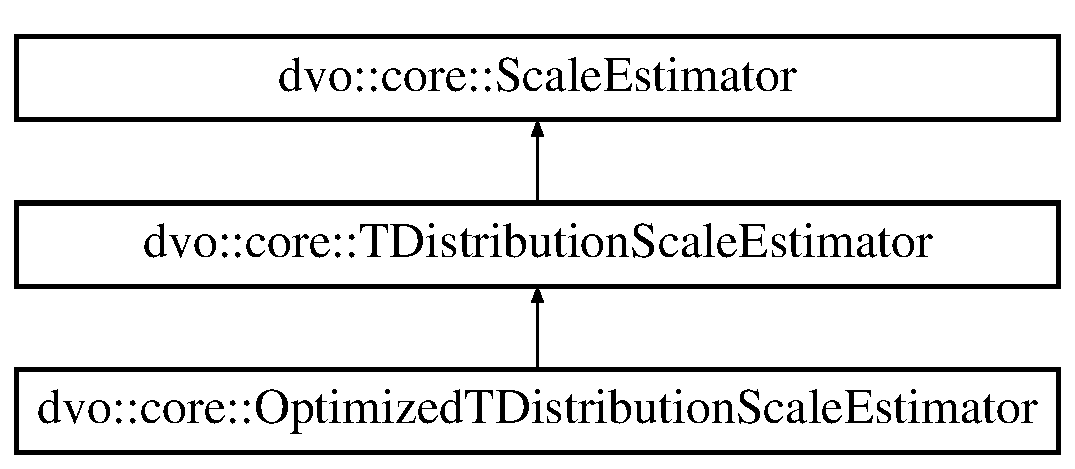
\includegraphics[height=3.000000cm]{classdvo_1_1core_1_1_optimized_t_distribution_scale_estimator}
\end{center}
\end{figure}
\subsection*{Public Member Functions}
\begin{DoxyCompactItemize}
\item 
\mbox{\hyperlink{classdvo_1_1core_1_1_optimized_t_distribution_scale_estimator_a05c83a7876c15949f24cb16c41ea2464}{Optimized\+T\+Distribution\+Scale\+Estimator}} (const float \mbox{\hyperlink{classdvo_1_1core_1_1_t_distribution_scale_estimator_a4c5ece510a3315bad7ca711a27466eb9}{dof}}=\mbox{\hyperlink{classdvo_1_1core_1_1_t_distribution_scale_estimator_a031ff291023c516c23bce04b34b79957}{D\+E\+F\+A\+U\+L\+T\+\_\+\+D\+OF}})
\item 
virtual \mbox{\hyperlink{classdvo_1_1core_1_1_optimized_t_distribution_scale_estimator_a929ac3c2914a6e150275a4d12ae8222c}{$\sim$\+Optimized\+T\+Distribution\+Scale\+Estimator}} ()
\item 
virtual float \mbox{\hyperlink{classdvo_1_1core_1_1_optimized_t_distribution_scale_estimator_ace9304a785bd16a6ef5cf4a52f3c6299}{compute}} (const cv\+::\+Mat \&errors) const
\end{DoxyCompactItemize}
\subsection*{Additional Inherited Members}


\subsection{Constructor \& Destructor Documentation}
\mbox{\Hypertarget{classdvo_1_1core_1_1_optimized_t_distribution_scale_estimator_a05c83a7876c15949f24cb16c41ea2464}\label{classdvo_1_1core_1_1_optimized_t_distribution_scale_estimator_a05c83a7876c15949f24cb16c41ea2464}} 
\index{dvo\+::core\+::\+Optimized\+T\+Distribution\+Scale\+Estimator@{dvo\+::core\+::\+Optimized\+T\+Distribution\+Scale\+Estimator}!Optimized\+T\+Distribution\+Scale\+Estimator@{Optimized\+T\+Distribution\+Scale\+Estimator}}
\index{Optimized\+T\+Distribution\+Scale\+Estimator@{Optimized\+T\+Distribution\+Scale\+Estimator}!dvo\+::core\+::\+Optimized\+T\+Distribution\+Scale\+Estimator@{dvo\+::core\+::\+Optimized\+T\+Distribution\+Scale\+Estimator}}
\subsubsection{\texorpdfstring{Optimized\+T\+Distribution\+Scale\+Estimator()}{OptimizedTDistributionScaleEstimator()}}
{\footnotesize\ttfamily dvo\+::core\+::\+Optimized\+T\+Distribution\+Scale\+Estimator\+::\+Optimized\+T\+Distribution\+Scale\+Estimator (\begin{DoxyParamCaption}\item[{const float}]{dof = {\ttfamily \mbox{\hyperlink{classdvo_1_1core_1_1_t_distribution_scale_estimator_a031ff291023c516c23bce04b34b79957}{D\+E\+F\+A\+U\+L\+T\+\_\+\+D\+OF}}} }\end{DoxyParamCaption})}

\mbox{\Hypertarget{classdvo_1_1core_1_1_optimized_t_distribution_scale_estimator_a929ac3c2914a6e150275a4d12ae8222c}\label{classdvo_1_1core_1_1_optimized_t_distribution_scale_estimator_a929ac3c2914a6e150275a4d12ae8222c}} 
\index{dvo\+::core\+::\+Optimized\+T\+Distribution\+Scale\+Estimator@{dvo\+::core\+::\+Optimized\+T\+Distribution\+Scale\+Estimator}!````~Optimized\+T\+Distribution\+Scale\+Estimator@{$\sim$\+Optimized\+T\+Distribution\+Scale\+Estimator}}
\index{````~Optimized\+T\+Distribution\+Scale\+Estimator@{$\sim$\+Optimized\+T\+Distribution\+Scale\+Estimator}!dvo\+::core\+::\+Optimized\+T\+Distribution\+Scale\+Estimator@{dvo\+::core\+::\+Optimized\+T\+Distribution\+Scale\+Estimator}}
\subsubsection{\texorpdfstring{$\sim$\+Optimized\+T\+Distribution\+Scale\+Estimator()}{~OptimizedTDistributionScaleEstimator()}}
{\footnotesize\ttfamily virtual dvo\+::core\+::\+Optimized\+T\+Distribution\+Scale\+Estimator\+::$\sim$\+Optimized\+T\+Distribution\+Scale\+Estimator (\begin{DoxyParamCaption}{ }\end{DoxyParamCaption})\hspace{0.3cm}{\ttfamily [inline]}, {\ttfamily [virtual]}}



\subsection{Member Function Documentation}
\mbox{\Hypertarget{classdvo_1_1core_1_1_optimized_t_distribution_scale_estimator_ace9304a785bd16a6ef5cf4a52f3c6299}\label{classdvo_1_1core_1_1_optimized_t_distribution_scale_estimator_ace9304a785bd16a6ef5cf4a52f3c6299}} 
\index{dvo\+::core\+::\+Optimized\+T\+Distribution\+Scale\+Estimator@{dvo\+::core\+::\+Optimized\+T\+Distribution\+Scale\+Estimator}!compute@{compute}}
\index{compute@{compute}!dvo\+::core\+::\+Optimized\+T\+Distribution\+Scale\+Estimator@{dvo\+::core\+::\+Optimized\+T\+Distribution\+Scale\+Estimator}}
\subsubsection{\texorpdfstring{compute()}{compute()}}
{\footnotesize\ttfamily float dvo\+::core\+::\+Optimized\+T\+Distribution\+Scale\+Estimator\+::compute (\begin{DoxyParamCaption}\item[{const cv\+::\+Mat \&}]{errors }\end{DoxyParamCaption}) const\hspace{0.3cm}{\ttfamily [virtual]}}



Reimplemented from \mbox{\hyperlink{classdvo_1_1core_1_1_t_distribution_scale_estimator_a0ed88ffeb9b71110e3ae69b681526bc4}{dvo\+::core\+::\+T\+Distribution\+Scale\+Estimator}}.



The documentation for this class was generated from the following files\+:\begin{DoxyCompactItemize}
\item 
dvo\+\_\+core/include/dvo/core/\mbox{\hyperlink{weight__calculation_8h}{weight\+\_\+calculation.\+h}}\item 
dvo\+\_\+core/src/core/\mbox{\hyperlink{weight__calculation_8cpp}{weight\+\_\+calculation.\+cpp}}\end{DoxyCompactItemize}

\hypertarget{classdvo_1_1visualization_1_1_pcl_camera_trajectory_visualizer}{}\section{dvo\+:\+:visualization\+:\+:Pcl\+Camera\+Trajectory\+Visualizer Class Reference}
\label{classdvo_1_1visualization_1_1_pcl_camera_trajectory_visualizer}\index{dvo\+::visualization\+::\+Pcl\+Camera\+Trajectory\+Visualizer@{dvo\+::visualization\+::\+Pcl\+Camera\+Trajectory\+Visualizer}}


{\ttfamily \#include $<$pcl\+\_\+camera\+\_\+trajectory\+\_\+visualizer.\+h$>$}

Inheritance diagram for dvo\+:\+:visualization\+:\+:Pcl\+Camera\+Trajectory\+Visualizer\+:\begin{figure}[H]
\begin{center}
\leavevmode
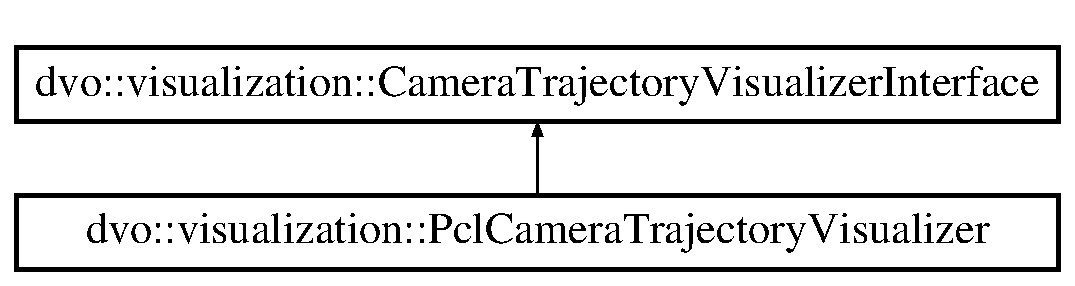
\includegraphics[height=2.000000cm]{classdvo_1_1visualization_1_1_pcl_camera_trajectory_visualizer}
\end{center}
\end{figure}
\subsection*{Public Member Functions}
\begin{DoxyCompactItemize}
\item 
\mbox{\hyperlink{classdvo_1_1visualization_1_1_pcl_camera_trajectory_visualizer_a9edc1a2e72987b2dcdf9493c087817cc}{Pcl\+Camera\+Trajectory\+Visualizer}} (bool async=true)
\item 
virtual \mbox{\hyperlink{classdvo_1_1visualization_1_1_pcl_camera_trajectory_visualizer_a541a106d21f43f3ce4d108bff79c64ea}{$\sim$\+Pcl\+Camera\+Trajectory\+Visualizer}} ()
\item 
virtual \mbox{\hyperlink{classdvo_1_1visualization_1_1_camera_visualizer_a473ebecc62e1d4edba21027d858789a2}{dvo\+::visualization\+::\+Camera\+Visualizer\+::\+Ptr}} \mbox{\hyperlink{classdvo_1_1visualization_1_1_pcl_camera_trajectory_visualizer_af808188bb664cdaac442f79fe67b40a6}{camera}} (std\+::string name)
\item 
virtual \mbox{\hyperlink{classdvo_1_1visualization_1_1_trajectory_visualizer_aac33ef5979fe64ee33409f1afa977fd3}{dvo\+::visualization\+::\+Trajectory\+Visualizer\+::\+Ptr}} \mbox{\hyperlink{classdvo_1_1visualization_1_1_pcl_camera_trajectory_visualizer_ad0ea0d8feefef54cd5dc15cd483b3610}{trajectory}} (std\+::string name)
\item 
virtual void \mbox{\hyperlink{classdvo_1_1visualization_1_1_pcl_camera_trajectory_visualizer_a1dd833071b1343a97c0366d3ced0799b}{reset}} ()
\item 
void \mbox{\hyperlink{classdvo_1_1visualization_1_1_pcl_camera_trajectory_visualizer_a7db9ae0e3abc85bcb8a5259df501154c}{bind\+Switch\+To\+Key}} (\mbox{\hyperlink{structdvo_1_1visualization_1_1_switch}{Switch}} \&s, std\+::string key)
\item 
void \mbox{\hyperlink{classdvo_1_1visualization_1_1_pcl_camera_trajectory_visualizer_a4d11076029980fdf3492da7eb304fe6a}{render}} (int milliseconds=15)
\item 
boost\+::mutex \& \mbox{\hyperlink{classdvo_1_1visualization_1_1_pcl_camera_trajectory_visualizer_a314dca78e0ea3b86e59dc9953bfd59f0}{sync}} ()
\item 
pcl\+::visualization\+::\+P\+C\+L\+Visualizer \& \mbox{\hyperlink{classdvo_1_1visualization_1_1_pcl_camera_trajectory_visualizer_a29266bd96578573e145d97d2574abd78}{visualizer}} ()
\end{DoxyCompactItemize}


\subsection{Constructor \& Destructor Documentation}
\mbox{\Hypertarget{classdvo_1_1visualization_1_1_pcl_camera_trajectory_visualizer_a9edc1a2e72987b2dcdf9493c087817cc}\label{classdvo_1_1visualization_1_1_pcl_camera_trajectory_visualizer_a9edc1a2e72987b2dcdf9493c087817cc}} 
\index{dvo\+::visualization\+::\+Pcl\+Camera\+Trajectory\+Visualizer@{dvo\+::visualization\+::\+Pcl\+Camera\+Trajectory\+Visualizer}!Pcl\+Camera\+Trajectory\+Visualizer@{Pcl\+Camera\+Trajectory\+Visualizer}}
\index{Pcl\+Camera\+Trajectory\+Visualizer@{Pcl\+Camera\+Trajectory\+Visualizer}!dvo\+::visualization\+::\+Pcl\+Camera\+Trajectory\+Visualizer@{dvo\+::visualization\+::\+Pcl\+Camera\+Trajectory\+Visualizer}}
\subsubsection{\texorpdfstring{Pcl\+Camera\+Trajectory\+Visualizer()}{PclCameraTrajectoryVisualizer()}}
{\footnotesize\ttfamily dvo\+::visualization\+::\+Pcl\+Camera\+Trajectory\+Visualizer\+::\+Pcl\+Camera\+Trajectory\+Visualizer (\begin{DoxyParamCaption}\item[{bool}]{async = {\ttfamily true} }\end{DoxyParamCaption})}

\mbox{\Hypertarget{classdvo_1_1visualization_1_1_pcl_camera_trajectory_visualizer_a541a106d21f43f3ce4d108bff79c64ea}\label{classdvo_1_1visualization_1_1_pcl_camera_trajectory_visualizer_a541a106d21f43f3ce4d108bff79c64ea}} 
\index{dvo\+::visualization\+::\+Pcl\+Camera\+Trajectory\+Visualizer@{dvo\+::visualization\+::\+Pcl\+Camera\+Trajectory\+Visualizer}!````~Pcl\+Camera\+Trajectory\+Visualizer@{$\sim$\+Pcl\+Camera\+Trajectory\+Visualizer}}
\index{````~Pcl\+Camera\+Trajectory\+Visualizer@{$\sim$\+Pcl\+Camera\+Trajectory\+Visualizer}!dvo\+::visualization\+::\+Pcl\+Camera\+Trajectory\+Visualizer@{dvo\+::visualization\+::\+Pcl\+Camera\+Trajectory\+Visualizer}}
\subsubsection{\texorpdfstring{$\sim$\+Pcl\+Camera\+Trajectory\+Visualizer()}{~PclCameraTrajectoryVisualizer()}}
{\footnotesize\ttfamily dvo\+::visualization\+::\+Pcl\+Camera\+Trajectory\+Visualizer\+::$\sim$\+Pcl\+Camera\+Trajectory\+Visualizer (\begin{DoxyParamCaption}{ }\end{DoxyParamCaption})\hspace{0.3cm}{\ttfamily [virtual]}}



\subsection{Member Function Documentation}
\mbox{\Hypertarget{classdvo_1_1visualization_1_1_pcl_camera_trajectory_visualizer_a7db9ae0e3abc85bcb8a5259df501154c}\label{classdvo_1_1visualization_1_1_pcl_camera_trajectory_visualizer_a7db9ae0e3abc85bcb8a5259df501154c}} 
\index{dvo\+::visualization\+::\+Pcl\+Camera\+Trajectory\+Visualizer@{dvo\+::visualization\+::\+Pcl\+Camera\+Trajectory\+Visualizer}!bind\+Switch\+To\+Key@{bind\+Switch\+To\+Key}}
\index{bind\+Switch\+To\+Key@{bind\+Switch\+To\+Key}!dvo\+::visualization\+::\+Pcl\+Camera\+Trajectory\+Visualizer@{dvo\+::visualization\+::\+Pcl\+Camera\+Trajectory\+Visualizer}}
\subsubsection{\texorpdfstring{bind\+Switch\+To\+Key()}{bindSwitchToKey()}}
{\footnotesize\ttfamily void dvo\+::visualization\+::\+Pcl\+Camera\+Trajectory\+Visualizer\+::bind\+Switch\+To\+Key (\begin{DoxyParamCaption}\item[{\mbox{\hyperlink{structdvo_1_1visualization_1_1_switch}{Switch}} \&}]{s,  }\item[{std\+::string}]{key }\end{DoxyParamCaption})}

\mbox{\Hypertarget{classdvo_1_1visualization_1_1_pcl_camera_trajectory_visualizer_af808188bb664cdaac442f79fe67b40a6}\label{classdvo_1_1visualization_1_1_pcl_camera_trajectory_visualizer_af808188bb664cdaac442f79fe67b40a6}} 
\index{dvo\+::visualization\+::\+Pcl\+Camera\+Trajectory\+Visualizer@{dvo\+::visualization\+::\+Pcl\+Camera\+Trajectory\+Visualizer}!camera@{camera}}
\index{camera@{camera}!dvo\+::visualization\+::\+Pcl\+Camera\+Trajectory\+Visualizer@{dvo\+::visualization\+::\+Pcl\+Camera\+Trajectory\+Visualizer}}
\subsubsection{\texorpdfstring{camera()}{camera()}}
{\footnotesize\ttfamily \mbox{\hyperlink{classdvo_1_1visualization_1_1_camera_visualizer_a473ebecc62e1d4edba21027d858789a2}{dvo\+::visualization\+::\+Camera\+Visualizer\+::\+Ptr}} dvo\+::visualization\+::\+Pcl\+Camera\+Trajectory\+Visualizer\+::camera (\begin{DoxyParamCaption}\item[{std\+::string}]{name }\end{DoxyParamCaption})\hspace{0.3cm}{\ttfamily [virtual]}}



Implements \mbox{\hyperlink{classdvo_1_1visualization_1_1_camera_trajectory_visualizer_interface_a4d43cd43f26bd880eb07e8ee37a7154a}{dvo\+::visualization\+::\+Camera\+Trajectory\+Visualizer\+Interface}}.

\mbox{\Hypertarget{classdvo_1_1visualization_1_1_pcl_camera_trajectory_visualizer_a4d11076029980fdf3492da7eb304fe6a}\label{classdvo_1_1visualization_1_1_pcl_camera_trajectory_visualizer_a4d11076029980fdf3492da7eb304fe6a}} 
\index{dvo\+::visualization\+::\+Pcl\+Camera\+Trajectory\+Visualizer@{dvo\+::visualization\+::\+Pcl\+Camera\+Trajectory\+Visualizer}!render@{render}}
\index{render@{render}!dvo\+::visualization\+::\+Pcl\+Camera\+Trajectory\+Visualizer@{dvo\+::visualization\+::\+Pcl\+Camera\+Trajectory\+Visualizer}}
\subsubsection{\texorpdfstring{render()}{render()}}
{\footnotesize\ttfamily void dvo\+::visualization\+::\+Pcl\+Camera\+Trajectory\+Visualizer\+::render (\begin{DoxyParamCaption}\item[{int}]{milliseconds = {\ttfamily 15} }\end{DoxyParamCaption})}

\mbox{\Hypertarget{classdvo_1_1visualization_1_1_pcl_camera_trajectory_visualizer_a1dd833071b1343a97c0366d3ced0799b}\label{classdvo_1_1visualization_1_1_pcl_camera_trajectory_visualizer_a1dd833071b1343a97c0366d3ced0799b}} 
\index{dvo\+::visualization\+::\+Pcl\+Camera\+Trajectory\+Visualizer@{dvo\+::visualization\+::\+Pcl\+Camera\+Trajectory\+Visualizer}!reset@{reset}}
\index{reset@{reset}!dvo\+::visualization\+::\+Pcl\+Camera\+Trajectory\+Visualizer@{dvo\+::visualization\+::\+Pcl\+Camera\+Trajectory\+Visualizer}}
\subsubsection{\texorpdfstring{reset()}{reset()}}
{\footnotesize\ttfamily void dvo\+::visualization\+::\+Pcl\+Camera\+Trajectory\+Visualizer\+::reset (\begin{DoxyParamCaption}{ }\end{DoxyParamCaption})\hspace{0.3cm}{\ttfamily [virtual]}}



Implements \mbox{\hyperlink{classdvo_1_1visualization_1_1_camera_trajectory_visualizer_interface_abcc7ddffc30b41eb9112c386f3e41aa7}{dvo\+::visualization\+::\+Camera\+Trajectory\+Visualizer\+Interface}}.

\mbox{\Hypertarget{classdvo_1_1visualization_1_1_pcl_camera_trajectory_visualizer_a314dca78e0ea3b86e59dc9953bfd59f0}\label{classdvo_1_1visualization_1_1_pcl_camera_trajectory_visualizer_a314dca78e0ea3b86e59dc9953bfd59f0}} 
\index{dvo\+::visualization\+::\+Pcl\+Camera\+Trajectory\+Visualizer@{dvo\+::visualization\+::\+Pcl\+Camera\+Trajectory\+Visualizer}!sync@{sync}}
\index{sync@{sync}!dvo\+::visualization\+::\+Pcl\+Camera\+Trajectory\+Visualizer@{dvo\+::visualization\+::\+Pcl\+Camera\+Trajectory\+Visualizer}}
\subsubsection{\texorpdfstring{sync()}{sync()}}
{\footnotesize\ttfamily boost\+::mutex \& dvo\+::visualization\+::\+Pcl\+Camera\+Trajectory\+Visualizer\+::sync (\begin{DoxyParamCaption}{ }\end{DoxyParamCaption})}

\mbox{\Hypertarget{classdvo_1_1visualization_1_1_pcl_camera_trajectory_visualizer_ad0ea0d8feefef54cd5dc15cd483b3610}\label{classdvo_1_1visualization_1_1_pcl_camera_trajectory_visualizer_ad0ea0d8feefef54cd5dc15cd483b3610}} 
\index{dvo\+::visualization\+::\+Pcl\+Camera\+Trajectory\+Visualizer@{dvo\+::visualization\+::\+Pcl\+Camera\+Trajectory\+Visualizer}!trajectory@{trajectory}}
\index{trajectory@{trajectory}!dvo\+::visualization\+::\+Pcl\+Camera\+Trajectory\+Visualizer@{dvo\+::visualization\+::\+Pcl\+Camera\+Trajectory\+Visualizer}}
\subsubsection{\texorpdfstring{trajectory()}{trajectory()}}
{\footnotesize\ttfamily \mbox{\hyperlink{classdvo_1_1visualization_1_1_trajectory_visualizer_aac33ef5979fe64ee33409f1afa977fd3}{dvo\+::visualization\+::\+Trajectory\+Visualizer\+::\+Ptr}} dvo\+::visualization\+::\+Pcl\+Camera\+Trajectory\+Visualizer\+::trajectory (\begin{DoxyParamCaption}\item[{std\+::string}]{name }\end{DoxyParamCaption})\hspace{0.3cm}{\ttfamily [virtual]}}



Implements \mbox{\hyperlink{classdvo_1_1visualization_1_1_camera_trajectory_visualizer_interface_ac658e841335e51c50325267de10e64b3}{dvo\+::visualization\+::\+Camera\+Trajectory\+Visualizer\+Interface}}.

\mbox{\Hypertarget{classdvo_1_1visualization_1_1_pcl_camera_trajectory_visualizer_a29266bd96578573e145d97d2574abd78}\label{classdvo_1_1visualization_1_1_pcl_camera_trajectory_visualizer_a29266bd96578573e145d97d2574abd78}} 
\index{dvo\+::visualization\+::\+Pcl\+Camera\+Trajectory\+Visualizer@{dvo\+::visualization\+::\+Pcl\+Camera\+Trajectory\+Visualizer}!visualizer@{visualizer}}
\index{visualizer@{visualizer}!dvo\+::visualization\+::\+Pcl\+Camera\+Trajectory\+Visualizer@{dvo\+::visualization\+::\+Pcl\+Camera\+Trajectory\+Visualizer}}
\subsubsection{\texorpdfstring{visualizer()}{visualizer()}}
{\footnotesize\ttfamily pcl\+::visualization\+::\+P\+C\+L\+Visualizer \& dvo\+::visualization\+::\+Pcl\+Camera\+Trajectory\+Visualizer\+::visualizer (\begin{DoxyParamCaption}{ }\end{DoxyParamCaption})}



The documentation for this class was generated from the following files\+:\begin{DoxyCompactItemize}
\item 
dvo\+\_\+core/include/dvo/visualization/\mbox{\hyperlink{pcl__camera__trajectory__visualizer_8h}{pcl\+\_\+camera\+\_\+trajectory\+\_\+visualizer.\+h}}\item 
dvo\+\_\+core/src/visualization/\mbox{\hyperlink{pcl__camera__trajetory__visualizer_8cpp}{pcl\+\_\+camera\+\_\+trajetory\+\_\+visualizer.\+cpp}}\end{DoxyCompactItemize}

\hypertarget{structdvo_1_1visualization_1_1internal_1_1_pcl_camera_trajectory_visualizer_impl}{}\section{dvo\+:\+:visualization\+:\+:internal\+:\+:Pcl\+Camera\+Trajectory\+Visualizer\+Impl Struct Reference}
\label{structdvo_1_1visualization_1_1internal_1_1_pcl_camera_trajectory_visualizer_impl}\index{dvo\+::visualization\+::internal\+::\+Pcl\+Camera\+Trajectory\+Visualizer\+Impl@{dvo\+::visualization\+::internal\+::\+Pcl\+Camera\+Trajectory\+Visualizer\+Impl}}
\subsection*{Public Types}
\begin{DoxyCompactItemize}
\item 
typedef boost\+::shared\+\_\+ptr$<$ \mbox{\hyperlink{classdvo_1_1visualization_1_1internal_1_1_pcl_camera_visualizer}{Pcl\+Camera\+Visualizer}} $>$ \mbox{\hyperlink{structdvo_1_1visualization_1_1internal_1_1_pcl_camera_trajectory_visualizer_impl_ae1f73988c3445cb504978879b5abd6b2}{Pcl\+Camera\+Visualizer\+Ptr}}
\item 
typedef boost\+::shared\+\_\+ptr$<$ \mbox{\hyperlink{classdvo_1_1visualization_1_1internal_1_1_pcl_trajectory_visualizer}{Pcl\+Trajectory\+Visualizer}} $>$ \mbox{\hyperlink{structdvo_1_1visualization_1_1internal_1_1_pcl_camera_trajectory_visualizer_impl_abefe7d40c9c28acf23b80fd55dc4a8bb}{Pcl\+Trajectory\+Visualizer\+Ptr}}
\item 
typedef std\+::map$<$ std\+::string, \mbox{\hyperlink{structdvo_1_1visualization_1_1internal_1_1_pcl_camera_trajectory_visualizer_impl_ae1f73988c3445cb504978879b5abd6b2}{Pcl\+Camera\+Visualizer\+Ptr}} $>$ \mbox{\hyperlink{structdvo_1_1visualization_1_1internal_1_1_pcl_camera_trajectory_visualizer_impl_a7d244b61749bfd33a2170d2fc8bfa8b3}{Camera\+Visualizer\+Map}}
\item 
typedef std\+::map$<$ std\+::string, \mbox{\hyperlink{structdvo_1_1visualization_1_1internal_1_1_pcl_camera_trajectory_visualizer_impl_abefe7d40c9c28acf23b80fd55dc4a8bb}{Pcl\+Trajectory\+Visualizer\+Ptr}} $>$ \mbox{\hyperlink{structdvo_1_1visualization_1_1internal_1_1_pcl_camera_trajectory_visualizer_impl_a97e643f8b8f24ab7e9b79b0961fd2af7}{Trajectory\+Visualizer\+Map}}
\end{DoxyCompactItemize}
\subsection*{Public Member Functions}
\begin{DoxyCompactItemize}
\item 
\mbox{\hyperlink{structdvo_1_1visualization_1_1internal_1_1_pcl_camera_trajectory_visualizer_impl_ac27a7fde4cc28672ebb5e65f80eb8865}{Pcl\+Camera\+Trajectory\+Visualizer\+Impl}} (bool render\+\_\+thread=true)
\item 
\mbox{\hyperlink{structdvo_1_1visualization_1_1internal_1_1_pcl_camera_trajectory_visualizer_impl_a3a8627e770ee2c18d07e79f921e60d16}{$\sim$\+Pcl\+Camera\+Trajectory\+Visualizer\+Impl}} ()
\item 
void \mbox{\hyperlink{structdvo_1_1visualization_1_1internal_1_1_pcl_camera_trajectory_visualizer_impl_a21c3f13d2d5ccb2f2913a08a421cd7fd}{bind\+Switch\+To\+Key}} (\mbox{\hyperlink{structdvo_1_1visualization_1_1_switch}{Switch}} \&s, std\+::string \&key)
\item 
pcl\+::visualization\+::\+P\+C\+L\+Visualizer \& \mbox{\hyperlink{structdvo_1_1visualization_1_1internal_1_1_pcl_camera_trajectory_visualizer_impl_a28159937aa1551faf546b827eddb3f44}{visualizer}} ()
\item 
\mbox{\hyperlink{classdvo_1_1visualization_1_1_camera_visualizer_a473ebecc62e1d4edba21027d858789a2}{Camera\+Visualizer\+::\+Ptr}} \mbox{\hyperlink{structdvo_1_1visualization_1_1internal_1_1_pcl_camera_trajectory_visualizer_impl_a1834a57c67d10cbeac37362c546d3575}{camera}} (std\+::string name)
\item 
\mbox{\hyperlink{classdvo_1_1visualization_1_1_trajectory_visualizer_aac33ef5979fe64ee33409f1afa977fd3}{Trajectory\+Visualizer\+::\+Ptr}} \mbox{\hyperlink{structdvo_1_1visualization_1_1internal_1_1_pcl_camera_trajectory_visualizer_impl_a603eeb0964ce83fff1e736003177661c}{trajectory}} (std\+::string name)
\item 
void \mbox{\hyperlink{structdvo_1_1visualization_1_1internal_1_1_pcl_camera_trajectory_visualizer_impl_a3b1dc7581be3c4e278d0a60678be494e}{reset}} ()
\item 
void \mbox{\hyperlink{structdvo_1_1visualization_1_1internal_1_1_pcl_camera_trajectory_visualizer_impl_a79a0458c9c30be3b18f9cbc3a0d4002f}{init\+Visualizer}} ()
\item 
void \mbox{\hyperlink{structdvo_1_1visualization_1_1internal_1_1_pcl_camera_trajectory_visualizer_impl_ae2b0083367d0b2955cf2f7adb18a1acb}{render}} (int milliseconds)
\end{DoxyCompactItemize}
\subsection*{Public Attributes}
\begin{DoxyCompactItemize}
\item 
boost\+::mutex \mbox{\hyperlink{structdvo_1_1visualization_1_1internal_1_1_pcl_camera_trajectory_visualizer_impl_add80c1ad58f55ec00c2ad0d08c0aaaac}{sync\+\_\+}}
\end{DoxyCompactItemize}


\subsection{Member Typedef Documentation}
\mbox{\Hypertarget{structdvo_1_1visualization_1_1internal_1_1_pcl_camera_trajectory_visualizer_impl_a7d244b61749bfd33a2170d2fc8bfa8b3}\label{structdvo_1_1visualization_1_1internal_1_1_pcl_camera_trajectory_visualizer_impl_a7d244b61749bfd33a2170d2fc8bfa8b3}} 
\index{dvo\+::visualization\+::internal\+::\+Pcl\+Camera\+Trajectory\+Visualizer\+Impl@{dvo\+::visualization\+::internal\+::\+Pcl\+Camera\+Trajectory\+Visualizer\+Impl}!Camera\+Visualizer\+Map@{Camera\+Visualizer\+Map}}
\index{Camera\+Visualizer\+Map@{Camera\+Visualizer\+Map}!dvo\+::visualization\+::internal\+::\+Pcl\+Camera\+Trajectory\+Visualizer\+Impl@{dvo\+::visualization\+::internal\+::\+Pcl\+Camera\+Trajectory\+Visualizer\+Impl}}
\subsubsection{\texorpdfstring{Camera\+Visualizer\+Map}{CameraVisualizerMap}}
{\footnotesize\ttfamily typedef std\+::map$<$std\+::string, \mbox{\hyperlink{structdvo_1_1visualization_1_1internal_1_1_pcl_camera_trajectory_visualizer_impl_ae1f73988c3445cb504978879b5abd6b2}{Pcl\+Camera\+Visualizer\+Ptr}}$>$ \mbox{\hyperlink{structdvo_1_1visualization_1_1internal_1_1_pcl_camera_trajectory_visualizer_impl_a7d244b61749bfd33a2170d2fc8bfa8b3}{dvo\+::visualization\+::internal\+::\+Pcl\+Camera\+Trajectory\+Visualizer\+Impl\+::\+Camera\+Visualizer\+Map}}}

\mbox{\Hypertarget{structdvo_1_1visualization_1_1internal_1_1_pcl_camera_trajectory_visualizer_impl_ae1f73988c3445cb504978879b5abd6b2}\label{structdvo_1_1visualization_1_1internal_1_1_pcl_camera_trajectory_visualizer_impl_ae1f73988c3445cb504978879b5abd6b2}} 
\index{dvo\+::visualization\+::internal\+::\+Pcl\+Camera\+Trajectory\+Visualizer\+Impl@{dvo\+::visualization\+::internal\+::\+Pcl\+Camera\+Trajectory\+Visualizer\+Impl}!Pcl\+Camera\+Visualizer\+Ptr@{Pcl\+Camera\+Visualizer\+Ptr}}
\index{Pcl\+Camera\+Visualizer\+Ptr@{Pcl\+Camera\+Visualizer\+Ptr}!dvo\+::visualization\+::internal\+::\+Pcl\+Camera\+Trajectory\+Visualizer\+Impl@{dvo\+::visualization\+::internal\+::\+Pcl\+Camera\+Trajectory\+Visualizer\+Impl}}
\subsubsection{\texorpdfstring{Pcl\+Camera\+Visualizer\+Ptr}{PclCameraVisualizerPtr}}
{\footnotesize\ttfamily typedef boost\+::shared\+\_\+ptr$<$\mbox{\hyperlink{classdvo_1_1visualization_1_1internal_1_1_pcl_camera_visualizer}{Pcl\+Camera\+Visualizer}}$>$ \mbox{\hyperlink{structdvo_1_1visualization_1_1internal_1_1_pcl_camera_trajectory_visualizer_impl_ae1f73988c3445cb504978879b5abd6b2}{dvo\+::visualization\+::internal\+::\+Pcl\+Camera\+Trajectory\+Visualizer\+Impl\+::\+Pcl\+Camera\+Visualizer\+Ptr}}}

\mbox{\Hypertarget{structdvo_1_1visualization_1_1internal_1_1_pcl_camera_trajectory_visualizer_impl_abefe7d40c9c28acf23b80fd55dc4a8bb}\label{structdvo_1_1visualization_1_1internal_1_1_pcl_camera_trajectory_visualizer_impl_abefe7d40c9c28acf23b80fd55dc4a8bb}} 
\index{dvo\+::visualization\+::internal\+::\+Pcl\+Camera\+Trajectory\+Visualizer\+Impl@{dvo\+::visualization\+::internal\+::\+Pcl\+Camera\+Trajectory\+Visualizer\+Impl}!Pcl\+Trajectory\+Visualizer\+Ptr@{Pcl\+Trajectory\+Visualizer\+Ptr}}
\index{Pcl\+Trajectory\+Visualizer\+Ptr@{Pcl\+Trajectory\+Visualizer\+Ptr}!dvo\+::visualization\+::internal\+::\+Pcl\+Camera\+Trajectory\+Visualizer\+Impl@{dvo\+::visualization\+::internal\+::\+Pcl\+Camera\+Trajectory\+Visualizer\+Impl}}
\subsubsection{\texorpdfstring{Pcl\+Trajectory\+Visualizer\+Ptr}{PclTrajectoryVisualizerPtr}}
{\footnotesize\ttfamily typedef boost\+::shared\+\_\+ptr$<$\mbox{\hyperlink{classdvo_1_1visualization_1_1internal_1_1_pcl_trajectory_visualizer}{Pcl\+Trajectory\+Visualizer}}$>$ \mbox{\hyperlink{structdvo_1_1visualization_1_1internal_1_1_pcl_camera_trajectory_visualizer_impl_abefe7d40c9c28acf23b80fd55dc4a8bb}{dvo\+::visualization\+::internal\+::\+Pcl\+Camera\+Trajectory\+Visualizer\+Impl\+::\+Pcl\+Trajectory\+Visualizer\+Ptr}}}

\mbox{\Hypertarget{structdvo_1_1visualization_1_1internal_1_1_pcl_camera_trajectory_visualizer_impl_a97e643f8b8f24ab7e9b79b0961fd2af7}\label{structdvo_1_1visualization_1_1internal_1_1_pcl_camera_trajectory_visualizer_impl_a97e643f8b8f24ab7e9b79b0961fd2af7}} 
\index{dvo\+::visualization\+::internal\+::\+Pcl\+Camera\+Trajectory\+Visualizer\+Impl@{dvo\+::visualization\+::internal\+::\+Pcl\+Camera\+Trajectory\+Visualizer\+Impl}!Trajectory\+Visualizer\+Map@{Trajectory\+Visualizer\+Map}}
\index{Trajectory\+Visualizer\+Map@{Trajectory\+Visualizer\+Map}!dvo\+::visualization\+::internal\+::\+Pcl\+Camera\+Trajectory\+Visualizer\+Impl@{dvo\+::visualization\+::internal\+::\+Pcl\+Camera\+Trajectory\+Visualizer\+Impl}}
\subsubsection{\texorpdfstring{Trajectory\+Visualizer\+Map}{TrajectoryVisualizerMap}}
{\footnotesize\ttfamily typedef std\+::map$<$std\+::string, \mbox{\hyperlink{structdvo_1_1visualization_1_1internal_1_1_pcl_camera_trajectory_visualizer_impl_abefe7d40c9c28acf23b80fd55dc4a8bb}{Pcl\+Trajectory\+Visualizer\+Ptr}}$>$ \mbox{\hyperlink{structdvo_1_1visualization_1_1internal_1_1_pcl_camera_trajectory_visualizer_impl_a97e643f8b8f24ab7e9b79b0961fd2af7}{dvo\+::visualization\+::internal\+::\+Pcl\+Camera\+Trajectory\+Visualizer\+Impl\+::\+Trajectory\+Visualizer\+Map}}}



\subsection{Constructor \& Destructor Documentation}
\mbox{\Hypertarget{structdvo_1_1visualization_1_1internal_1_1_pcl_camera_trajectory_visualizer_impl_ac27a7fde4cc28672ebb5e65f80eb8865}\label{structdvo_1_1visualization_1_1internal_1_1_pcl_camera_trajectory_visualizer_impl_ac27a7fde4cc28672ebb5e65f80eb8865}} 
\index{dvo\+::visualization\+::internal\+::\+Pcl\+Camera\+Trajectory\+Visualizer\+Impl@{dvo\+::visualization\+::internal\+::\+Pcl\+Camera\+Trajectory\+Visualizer\+Impl}!Pcl\+Camera\+Trajectory\+Visualizer\+Impl@{Pcl\+Camera\+Trajectory\+Visualizer\+Impl}}
\index{Pcl\+Camera\+Trajectory\+Visualizer\+Impl@{Pcl\+Camera\+Trajectory\+Visualizer\+Impl}!dvo\+::visualization\+::internal\+::\+Pcl\+Camera\+Trajectory\+Visualizer\+Impl@{dvo\+::visualization\+::internal\+::\+Pcl\+Camera\+Trajectory\+Visualizer\+Impl}}
\subsubsection{\texorpdfstring{Pcl\+Camera\+Trajectory\+Visualizer\+Impl()}{PclCameraTrajectoryVisualizerImpl()}}
{\footnotesize\ttfamily dvo\+::visualization\+::internal\+::\+Pcl\+Camera\+Trajectory\+Visualizer\+Impl\+::\+Pcl\+Camera\+Trajectory\+Visualizer\+Impl (\begin{DoxyParamCaption}\item[{bool}]{render\+\_\+thread = {\ttfamily true} }\end{DoxyParamCaption})\hspace{0.3cm}{\ttfamily [inline]}}

\mbox{\Hypertarget{structdvo_1_1visualization_1_1internal_1_1_pcl_camera_trajectory_visualizer_impl_a3a8627e770ee2c18d07e79f921e60d16}\label{structdvo_1_1visualization_1_1internal_1_1_pcl_camera_trajectory_visualizer_impl_a3a8627e770ee2c18d07e79f921e60d16}} 
\index{dvo\+::visualization\+::internal\+::\+Pcl\+Camera\+Trajectory\+Visualizer\+Impl@{dvo\+::visualization\+::internal\+::\+Pcl\+Camera\+Trajectory\+Visualizer\+Impl}!````~Pcl\+Camera\+Trajectory\+Visualizer\+Impl@{$\sim$\+Pcl\+Camera\+Trajectory\+Visualizer\+Impl}}
\index{````~Pcl\+Camera\+Trajectory\+Visualizer\+Impl@{$\sim$\+Pcl\+Camera\+Trajectory\+Visualizer\+Impl}!dvo\+::visualization\+::internal\+::\+Pcl\+Camera\+Trajectory\+Visualizer\+Impl@{dvo\+::visualization\+::internal\+::\+Pcl\+Camera\+Trajectory\+Visualizer\+Impl}}
\subsubsection{\texorpdfstring{$\sim$\+Pcl\+Camera\+Trajectory\+Visualizer\+Impl()}{~PclCameraTrajectoryVisualizerImpl()}}
{\footnotesize\ttfamily dvo\+::visualization\+::internal\+::\+Pcl\+Camera\+Trajectory\+Visualizer\+Impl\+::$\sim$\+Pcl\+Camera\+Trajectory\+Visualizer\+Impl (\begin{DoxyParamCaption}{ }\end{DoxyParamCaption})\hspace{0.3cm}{\ttfamily [inline]}}



\subsection{Member Function Documentation}
\mbox{\Hypertarget{structdvo_1_1visualization_1_1internal_1_1_pcl_camera_trajectory_visualizer_impl_a21c3f13d2d5ccb2f2913a08a421cd7fd}\label{structdvo_1_1visualization_1_1internal_1_1_pcl_camera_trajectory_visualizer_impl_a21c3f13d2d5ccb2f2913a08a421cd7fd}} 
\index{dvo\+::visualization\+::internal\+::\+Pcl\+Camera\+Trajectory\+Visualizer\+Impl@{dvo\+::visualization\+::internal\+::\+Pcl\+Camera\+Trajectory\+Visualizer\+Impl}!bind\+Switch\+To\+Key@{bind\+Switch\+To\+Key}}
\index{bind\+Switch\+To\+Key@{bind\+Switch\+To\+Key}!dvo\+::visualization\+::internal\+::\+Pcl\+Camera\+Trajectory\+Visualizer\+Impl@{dvo\+::visualization\+::internal\+::\+Pcl\+Camera\+Trajectory\+Visualizer\+Impl}}
\subsubsection{\texorpdfstring{bind\+Switch\+To\+Key()}{bindSwitchToKey()}}
{\footnotesize\ttfamily void dvo\+::visualization\+::internal\+::\+Pcl\+Camera\+Trajectory\+Visualizer\+Impl\+::bind\+Switch\+To\+Key (\begin{DoxyParamCaption}\item[{\mbox{\hyperlink{structdvo_1_1visualization_1_1_switch}{Switch}} \&}]{s,  }\item[{std\+::string \&}]{key }\end{DoxyParamCaption})\hspace{0.3cm}{\ttfamily [inline]}}

\mbox{\Hypertarget{structdvo_1_1visualization_1_1internal_1_1_pcl_camera_trajectory_visualizer_impl_a1834a57c67d10cbeac37362c546d3575}\label{structdvo_1_1visualization_1_1internal_1_1_pcl_camera_trajectory_visualizer_impl_a1834a57c67d10cbeac37362c546d3575}} 
\index{dvo\+::visualization\+::internal\+::\+Pcl\+Camera\+Trajectory\+Visualizer\+Impl@{dvo\+::visualization\+::internal\+::\+Pcl\+Camera\+Trajectory\+Visualizer\+Impl}!camera@{camera}}
\index{camera@{camera}!dvo\+::visualization\+::internal\+::\+Pcl\+Camera\+Trajectory\+Visualizer\+Impl@{dvo\+::visualization\+::internal\+::\+Pcl\+Camera\+Trajectory\+Visualizer\+Impl}}
\subsubsection{\texorpdfstring{camera()}{camera()}}
{\footnotesize\ttfamily \mbox{\hyperlink{classdvo_1_1visualization_1_1_camera_visualizer_a473ebecc62e1d4edba21027d858789a2}{Camera\+Visualizer\+::\+Ptr}} dvo\+::visualization\+::internal\+::\+Pcl\+Camera\+Trajectory\+Visualizer\+Impl\+::camera (\begin{DoxyParamCaption}\item[{std\+::string}]{name }\end{DoxyParamCaption})\hspace{0.3cm}{\ttfamily [inline]}}

\mbox{\Hypertarget{structdvo_1_1visualization_1_1internal_1_1_pcl_camera_trajectory_visualizer_impl_a79a0458c9c30be3b18f9cbc3a0d4002f}\label{structdvo_1_1visualization_1_1internal_1_1_pcl_camera_trajectory_visualizer_impl_a79a0458c9c30be3b18f9cbc3a0d4002f}} 
\index{dvo\+::visualization\+::internal\+::\+Pcl\+Camera\+Trajectory\+Visualizer\+Impl@{dvo\+::visualization\+::internal\+::\+Pcl\+Camera\+Trajectory\+Visualizer\+Impl}!init\+Visualizer@{init\+Visualizer}}
\index{init\+Visualizer@{init\+Visualizer}!dvo\+::visualization\+::internal\+::\+Pcl\+Camera\+Trajectory\+Visualizer\+Impl@{dvo\+::visualization\+::internal\+::\+Pcl\+Camera\+Trajectory\+Visualizer\+Impl}}
\subsubsection{\texorpdfstring{init\+Visualizer()}{initVisualizer()}}
{\footnotesize\ttfamily void dvo\+::visualization\+::internal\+::\+Pcl\+Camera\+Trajectory\+Visualizer\+Impl\+::init\+Visualizer (\begin{DoxyParamCaption}{ }\end{DoxyParamCaption})\hspace{0.3cm}{\ttfamily [inline]}}

\mbox{\Hypertarget{structdvo_1_1visualization_1_1internal_1_1_pcl_camera_trajectory_visualizer_impl_ae2b0083367d0b2955cf2f7adb18a1acb}\label{structdvo_1_1visualization_1_1internal_1_1_pcl_camera_trajectory_visualizer_impl_ae2b0083367d0b2955cf2f7adb18a1acb}} 
\index{dvo\+::visualization\+::internal\+::\+Pcl\+Camera\+Trajectory\+Visualizer\+Impl@{dvo\+::visualization\+::internal\+::\+Pcl\+Camera\+Trajectory\+Visualizer\+Impl}!render@{render}}
\index{render@{render}!dvo\+::visualization\+::internal\+::\+Pcl\+Camera\+Trajectory\+Visualizer\+Impl@{dvo\+::visualization\+::internal\+::\+Pcl\+Camera\+Trajectory\+Visualizer\+Impl}}
\subsubsection{\texorpdfstring{render()}{render()}}
{\footnotesize\ttfamily void dvo\+::visualization\+::internal\+::\+Pcl\+Camera\+Trajectory\+Visualizer\+Impl\+::render (\begin{DoxyParamCaption}\item[{int}]{milliseconds }\end{DoxyParamCaption})\hspace{0.3cm}{\ttfamily [inline]}}

\mbox{\Hypertarget{structdvo_1_1visualization_1_1internal_1_1_pcl_camera_trajectory_visualizer_impl_a3b1dc7581be3c4e278d0a60678be494e}\label{structdvo_1_1visualization_1_1internal_1_1_pcl_camera_trajectory_visualizer_impl_a3b1dc7581be3c4e278d0a60678be494e}} 
\index{dvo\+::visualization\+::internal\+::\+Pcl\+Camera\+Trajectory\+Visualizer\+Impl@{dvo\+::visualization\+::internal\+::\+Pcl\+Camera\+Trajectory\+Visualizer\+Impl}!reset@{reset}}
\index{reset@{reset}!dvo\+::visualization\+::internal\+::\+Pcl\+Camera\+Trajectory\+Visualizer\+Impl@{dvo\+::visualization\+::internal\+::\+Pcl\+Camera\+Trajectory\+Visualizer\+Impl}}
\subsubsection{\texorpdfstring{reset()}{reset()}}
{\footnotesize\ttfamily void dvo\+::visualization\+::internal\+::\+Pcl\+Camera\+Trajectory\+Visualizer\+Impl\+::reset (\begin{DoxyParamCaption}{ }\end{DoxyParamCaption})\hspace{0.3cm}{\ttfamily [inline]}}

\mbox{\Hypertarget{structdvo_1_1visualization_1_1internal_1_1_pcl_camera_trajectory_visualizer_impl_a603eeb0964ce83fff1e736003177661c}\label{structdvo_1_1visualization_1_1internal_1_1_pcl_camera_trajectory_visualizer_impl_a603eeb0964ce83fff1e736003177661c}} 
\index{dvo\+::visualization\+::internal\+::\+Pcl\+Camera\+Trajectory\+Visualizer\+Impl@{dvo\+::visualization\+::internal\+::\+Pcl\+Camera\+Trajectory\+Visualizer\+Impl}!trajectory@{trajectory}}
\index{trajectory@{trajectory}!dvo\+::visualization\+::internal\+::\+Pcl\+Camera\+Trajectory\+Visualizer\+Impl@{dvo\+::visualization\+::internal\+::\+Pcl\+Camera\+Trajectory\+Visualizer\+Impl}}
\subsubsection{\texorpdfstring{trajectory()}{trajectory()}}
{\footnotesize\ttfamily \mbox{\hyperlink{classdvo_1_1visualization_1_1_trajectory_visualizer_aac33ef5979fe64ee33409f1afa977fd3}{Trajectory\+Visualizer\+::\+Ptr}} dvo\+::visualization\+::internal\+::\+Pcl\+Camera\+Trajectory\+Visualizer\+Impl\+::trajectory (\begin{DoxyParamCaption}\item[{std\+::string}]{name }\end{DoxyParamCaption})\hspace{0.3cm}{\ttfamily [inline]}}

\mbox{\Hypertarget{structdvo_1_1visualization_1_1internal_1_1_pcl_camera_trajectory_visualizer_impl_a28159937aa1551faf546b827eddb3f44}\label{structdvo_1_1visualization_1_1internal_1_1_pcl_camera_trajectory_visualizer_impl_a28159937aa1551faf546b827eddb3f44}} 
\index{dvo\+::visualization\+::internal\+::\+Pcl\+Camera\+Trajectory\+Visualizer\+Impl@{dvo\+::visualization\+::internal\+::\+Pcl\+Camera\+Trajectory\+Visualizer\+Impl}!visualizer@{visualizer}}
\index{visualizer@{visualizer}!dvo\+::visualization\+::internal\+::\+Pcl\+Camera\+Trajectory\+Visualizer\+Impl@{dvo\+::visualization\+::internal\+::\+Pcl\+Camera\+Trajectory\+Visualizer\+Impl}}
\subsubsection{\texorpdfstring{visualizer()}{visualizer()}}
{\footnotesize\ttfamily pcl\+::visualization\+::\+P\+C\+L\+Visualizer\& dvo\+::visualization\+::internal\+::\+Pcl\+Camera\+Trajectory\+Visualizer\+Impl\+::visualizer (\begin{DoxyParamCaption}{ }\end{DoxyParamCaption})\hspace{0.3cm}{\ttfamily [inline]}}



\subsection{Member Data Documentation}
\mbox{\Hypertarget{structdvo_1_1visualization_1_1internal_1_1_pcl_camera_trajectory_visualizer_impl_add80c1ad58f55ec00c2ad0d08c0aaaac}\label{structdvo_1_1visualization_1_1internal_1_1_pcl_camera_trajectory_visualizer_impl_add80c1ad58f55ec00c2ad0d08c0aaaac}} 
\index{dvo\+::visualization\+::internal\+::\+Pcl\+Camera\+Trajectory\+Visualizer\+Impl@{dvo\+::visualization\+::internal\+::\+Pcl\+Camera\+Trajectory\+Visualizer\+Impl}!sync\+\_\+@{sync\+\_\+}}
\index{sync\+\_\+@{sync\+\_\+}!dvo\+::visualization\+::internal\+::\+Pcl\+Camera\+Trajectory\+Visualizer\+Impl@{dvo\+::visualization\+::internal\+::\+Pcl\+Camera\+Trajectory\+Visualizer\+Impl}}
\subsubsection{\texorpdfstring{sync\+\_\+}{sync\_}}
{\footnotesize\ttfamily boost\+::mutex dvo\+::visualization\+::internal\+::\+Pcl\+Camera\+Trajectory\+Visualizer\+Impl\+::sync\+\_\+}



The documentation for this struct was generated from the following file\+:\begin{DoxyCompactItemize}
\item 
dvo\+\_\+core/src/visualization/\mbox{\hyperlink{pcl__camera__trajetory__visualizer_8cpp}{pcl\+\_\+camera\+\_\+trajetory\+\_\+visualizer.\+cpp}}\end{DoxyCompactItemize}

\hypertarget{classdvo_1_1visualization_1_1internal_1_1_pcl_camera_visualizer}{}\section{dvo\+:\+:visualization\+:\+:internal\+:\+:Pcl\+Camera\+Visualizer Class Reference}
\label{classdvo_1_1visualization_1_1internal_1_1_pcl_camera_visualizer}\index{dvo\+::visualization\+::internal\+::\+Pcl\+Camera\+Visualizer@{dvo\+::visualization\+::internal\+::\+Pcl\+Camera\+Visualizer}}
Inheritance diagram for dvo\+:\+:visualization\+:\+:internal\+:\+:Pcl\+Camera\+Visualizer\+:\begin{figure}[H]
\begin{center}
\leavevmode
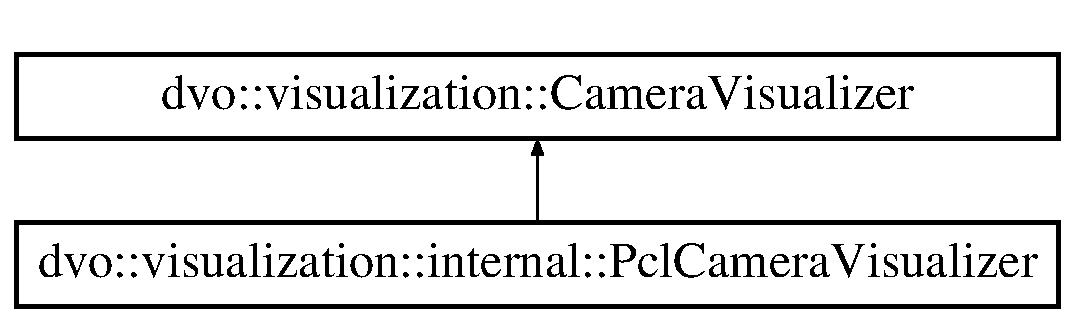
\includegraphics[height=2.000000cm]{classdvo_1_1visualization_1_1internal_1_1_pcl_camera_visualizer}
\end{center}
\end{figure}
\subsection*{Public Member Functions}
\begin{DoxyCompactItemize}
\item 
\mbox{\hyperlink{classdvo_1_1visualization_1_1internal_1_1_pcl_camera_visualizer_a4990540496b6a8104b6f3d794ed2bb17}{Pcl\+Camera\+Visualizer}} (std\+::string \&name)
\item 
virtual \mbox{\hyperlink{classdvo_1_1visualization_1_1internal_1_1_pcl_camera_visualizer_a594001de77ac60de8cd05a03d1314b8e}{$\sim$\+Pcl\+Camera\+Visualizer}} ()
\item 
virtual void \mbox{\hyperlink{classdvo_1_1visualization_1_1internal_1_1_pcl_camera_visualizer_a09b5d8117f8ca15489ac42f6b6019030}{show}} (\mbox{\hyperlink{classdvo_1_1visualization_1_1_camera_visualizer_a0526f50be9f298c4f7d1f91018d50af7}{Option}} option=\mbox{\hyperlink{classdvo_1_1visualization_1_1_camera_visualizer_a0526f50be9f298c4f7d1f91018d50af7a0ff8fc7d7283f27066e93ca0d4ef3f19}{Show\+Camera\+And\+Cloud}})
\item 
virtual void \mbox{\hyperlink{classdvo_1_1visualization_1_1internal_1_1_pcl_camera_visualizer_ad261307239a87bc10ba4d0662960cc72}{hide}} ()
\item 
virtual \mbox{\hyperlink{classdvo_1_1visualization_1_1_camera_visualizer}{Camera\+Visualizer}} \& \mbox{\hyperlink{classdvo_1_1visualization_1_1internal_1_1_pcl_camera_visualizer_adfe2b8752f78ee0fa6ee193be70941eb}{update}} (const \mbox{\hyperlink{structdvo_1_1core_1_1_rgbd_image}{dvo\+::core\+::\+Rgbd\+Image}} \&img, const \mbox{\hyperlink{structdvo_1_1core_1_1_intrinsic_matrix}{dvo\+::core\+::\+Intrinsic\+Matrix}} \&intrinsics, const Eigen\+::\+Affine3d \&pose)
\item 
void \mbox{\hyperlink{classdvo_1_1visualization_1_1internal_1_1_pcl_camera_visualizer_adbc6ea5a07dace4e06773d568986424b}{update\+Visualizer}} (pcl\+::visualization\+::\+P\+C\+L\+Visualizer \&visualizer, \mbox{\hyperlink{classdvo_1_1visualization_1_1_point_cloud_aggregator}{Point\+Cloud\+Aggregator}} \&aggregator)
\end{DoxyCompactItemize}
\subsection*{Additional Inherited Members}


\subsection{Constructor \& Destructor Documentation}
\mbox{\Hypertarget{classdvo_1_1visualization_1_1internal_1_1_pcl_camera_visualizer_a4990540496b6a8104b6f3d794ed2bb17}\label{classdvo_1_1visualization_1_1internal_1_1_pcl_camera_visualizer_a4990540496b6a8104b6f3d794ed2bb17}} 
\index{dvo\+::visualization\+::internal\+::\+Pcl\+Camera\+Visualizer@{dvo\+::visualization\+::internal\+::\+Pcl\+Camera\+Visualizer}!Pcl\+Camera\+Visualizer@{Pcl\+Camera\+Visualizer}}
\index{Pcl\+Camera\+Visualizer@{Pcl\+Camera\+Visualizer}!dvo\+::visualization\+::internal\+::\+Pcl\+Camera\+Visualizer@{dvo\+::visualization\+::internal\+::\+Pcl\+Camera\+Visualizer}}
\subsubsection{\texorpdfstring{Pcl\+Camera\+Visualizer()}{PclCameraVisualizer()}}
{\footnotesize\ttfamily dvo\+::visualization\+::internal\+::\+Pcl\+Camera\+Visualizer\+::\+Pcl\+Camera\+Visualizer (\begin{DoxyParamCaption}\item[{std\+::string \&}]{name }\end{DoxyParamCaption})\hspace{0.3cm}{\ttfamily [inline]}}

\mbox{\Hypertarget{classdvo_1_1visualization_1_1internal_1_1_pcl_camera_visualizer_a594001de77ac60de8cd05a03d1314b8e}\label{classdvo_1_1visualization_1_1internal_1_1_pcl_camera_visualizer_a594001de77ac60de8cd05a03d1314b8e}} 
\index{dvo\+::visualization\+::internal\+::\+Pcl\+Camera\+Visualizer@{dvo\+::visualization\+::internal\+::\+Pcl\+Camera\+Visualizer}!````~Pcl\+Camera\+Visualizer@{$\sim$\+Pcl\+Camera\+Visualizer}}
\index{````~Pcl\+Camera\+Visualizer@{$\sim$\+Pcl\+Camera\+Visualizer}!dvo\+::visualization\+::internal\+::\+Pcl\+Camera\+Visualizer@{dvo\+::visualization\+::internal\+::\+Pcl\+Camera\+Visualizer}}
\subsubsection{\texorpdfstring{$\sim$\+Pcl\+Camera\+Visualizer()}{~PclCameraVisualizer()}}
{\footnotesize\ttfamily virtual dvo\+::visualization\+::internal\+::\+Pcl\+Camera\+Visualizer\+::$\sim$\+Pcl\+Camera\+Visualizer (\begin{DoxyParamCaption}{ }\end{DoxyParamCaption})\hspace{0.3cm}{\ttfamily [inline]}, {\ttfamily [virtual]}}



\subsection{Member Function Documentation}
\mbox{\Hypertarget{classdvo_1_1visualization_1_1internal_1_1_pcl_camera_visualizer_ad261307239a87bc10ba4d0662960cc72}\label{classdvo_1_1visualization_1_1internal_1_1_pcl_camera_visualizer_ad261307239a87bc10ba4d0662960cc72}} 
\index{dvo\+::visualization\+::internal\+::\+Pcl\+Camera\+Visualizer@{dvo\+::visualization\+::internal\+::\+Pcl\+Camera\+Visualizer}!hide@{hide}}
\index{hide@{hide}!dvo\+::visualization\+::internal\+::\+Pcl\+Camera\+Visualizer@{dvo\+::visualization\+::internal\+::\+Pcl\+Camera\+Visualizer}}
\subsubsection{\texorpdfstring{hide()}{hide()}}
{\footnotesize\ttfamily virtual void dvo\+::visualization\+::internal\+::\+Pcl\+Camera\+Visualizer\+::hide (\begin{DoxyParamCaption}{ }\end{DoxyParamCaption})\hspace{0.3cm}{\ttfamily [inline]}, {\ttfamily [virtual]}}



Implements \mbox{\hyperlink{classdvo_1_1visualization_1_1_camera_visualizer_a45dbf0d449a7b7529f7da477c676ca85}{dvo\+::visualization\+::\+Camera\+Visualizer}}.

\mbox{\Hypertarget{classdvo_1_1visualization_1_1internal_1_1_pcl_camera_visualizer_a09b5d8117f8ca15489ac42f6b6019030}\label{classdvo_1_1visualization_1_1internal_1_1_pcl_camera_visualizer_a09b5d8117f8ca15489ac42f6b6019030}} 
\index{dvo\+::visualization\+::internal\+::\+Pcl\+Camera\+Visualizer@{dvo\+::visualization\+::internal\+::\+Pcl\+Camera\+Visualizer}!show@{show}}
\index{show@{show}!dvo\+::visualization\+::internal\+::\+Pcl\+Camera\+Visualizer@{dvo\+::visualization\+::internal\+::\+Pcl\+Camera\+Visualizer}}
\subsubsection{\texorpdfstring{show()}{show()}}
{\footnotesize\ttfamily virtual void dvo\+::visualization\+::internal\+::\+Pcl\+Camera\+Visualizer\+::show (\begin{DoxyParamCaption}\item[{\mbox{\hyperlink{classdvo_1_1visualization_1_1_camera_visualizer_a0526f50be9f298c4f7d1f91018d50af7}{Option}}}]{option = {\ttfamily \mbox{\hyperlink{classdvo_1_1visualization_1_1_camera_visualizer_a0526f50be9f298c4f7d1f91018d50af7a0ff8fc7d7283f27066e93ca0d4ef3f19}{Show\+Camera\+And\+Cloud}}} }\end{DoxyParamCaption})\hspace{0.3cm}{\ttfamily [inline]}, {\ttfamily [virtual]}}



Implements \mbox{\hyperlink{classdvo_1_1visualization_1_1_camera_visualizer_a646b21ea800d07f6a4174c80daf2bf50}{dvo\+::visualization\+::\+Camera\+Visualizer}}.

\mbox{\Hypertarget{classdvo_1_1visualization_1_1internal_1_1_pcl_camera_visualizer_adfe2b8752f78ee0fa6ee193be70941eb}\label{classdvo_1_1visualization_1_1internal_1_1_pcl_camera_visualizer_adfe2b8752f78ee0fa6ee193be70941eb}} 
\index{dvo\+::visualization\+::internal\+::\+Pcl\+Camera\+Visualizer@{dvo\+::visualization\+::internal\+::\+Pcl\+Camera\+Visualizer}!update@{update}}
\index{update@{update}!dvo\+::visualization\+::internal\+::\+Pcl\+Camera\+Visualizer@{dvo\+::visualization\+::internal\+::\+Pcl\+Camera\+Visualizer}}
\subsubsection{\texorpdfstring{update()}{update()}}
{\footnotesize\ttfamily virtual \mbox{\hyperlink{classdvo_1_1visualization_1_1_camera_visualizer}{Camera\+Visualizer}}\& dvo\+::visualization\+::internal\+::\+Pcl\+Camera\+Visualizer\+::update (\begin{DoxyParamCaption}\item[{const \mbox{\hyperlink{structdvo_1_1core_1_1_rgbd_image}{dvo\+::core\+::\+Rgbd\+Image}} \&}]{img,  }\item[{const \mbox{\hyperlink{structdvo_1_1core_1_1_intrinsic_matrix}{dvo\+::core\+::\+Intrinsic\+Matrix}} \&}]{intrinsics,  }\item[{const Eigen\+::\+Affine3d \&}]{pose }\end{DoxyParamCaption})\hspace{0.3cm}{\ttfamily [inline]}, {\ttfamily [virtual]}}



Implements \mbox{\hyperlink{classdvo_1_1visualization_1_1_camera_visualizer_afd83119e63048b0229820045d54c95ec}{dvo\+::visualization\+::\+Camera\+Visualizer}}.

\mbox{\Hypertarget{classdvo_1_1visualization_1_1internal_1_1_pcl_camera_visualizer_adbc6ea5a07dace4e06773d568986424b}\label{classdvo_1_1visualization_1_1internal_1_1_pcl_camera_visualizer_adbc6ea5a07dace4e06773d568986424b}} 
\index{dvo\+::visualization\+::internal\+::\+Pcl\+Camera\+Visualizer@{dvo\+::visualization\+::internal\+::\+Pcl\+Camera\+Visualizer}!update\+Visualizer@{update\+Visualizer}}
\index{update\+Visualizer@{update\+Visualizer}!dvo\+::visualization\+::internal\+::\+Pcl\+Camera\+Visualizer@{dvo\+::visualization\+::internal\+::\+Pcl\+Camera\+Visualizer}}
\subsubsection{\texorpdfstring{update\+Visualizer()}{updateVisualizer()}}
{\footnotesize\ttfamily void dvo\+::visualization\+::internal\+::\+Pcl\+Camera\+Visualizer\+::update\+Visualizer (\begin{DoxyParamCaption}\item[{pcl\+::visualization\+::\+P\+C\+L\+Visualizer \&}]{visualizer,  }\item[{\mbox{\hyperlink{classdvo_1_1visualization_1_1_point_cloud_aggregator}{Point\+Cloud\+Aggregator}} \&}]{aggregator }\end{DoxyParamCaption})\hspace{0.3cm}{\ttfamily [inline]}}



The documentation for this class was generated from the following file\+:\begin{DoxyCompactItemize}
\item 
dvo\+\_\+core/src/visualization/\mbox{\hyperlink{pcl__camera__trajetory__visualizer_8cpp}{pcl\+\_\+camera\+\_\+trajetory\+\_\+visualizer.\+cpp}}\end{DoxyCompactItemize}

\hypertarget{classdvo_1_1visualization_1_1internal_1_1_pcl_trajectory_visualizer}{}\section{dvo\+:\+:visualization\+:\+:internal\+:\+:Pcl\+Trajectory\+Visualizer Class Reference}
\label{classdvo_1_1visualization_1_1internal_1_1_pcl_trajectory_visualizer}\index{dvo\+::visualization\+::internal\+::\+Pcl\+Trajectory\+Visualizer@{dvo\+::visualization\+::internal\+::\+Pcl\+Trajectory\+Visualizer}}
Inheritance diagram for dvo\+:\+:visualization\+:\+:internal\+:\+:Pcl\+Trajectory\+Visualizer\+:\begin{figure}[H]
\begin{center}
\leavevmode
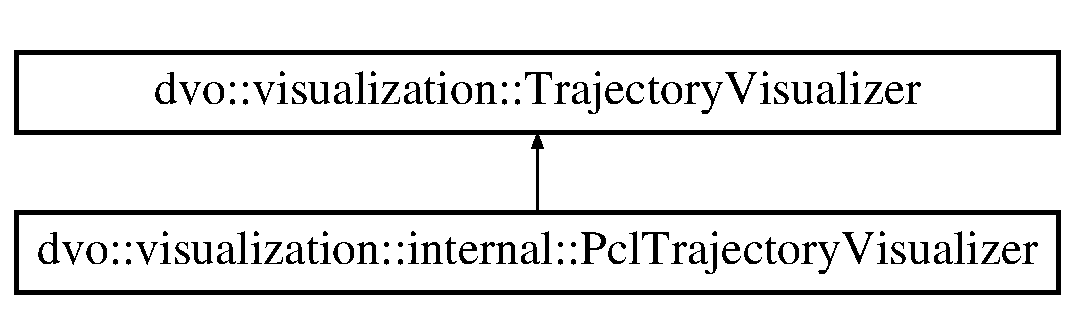
\includegraphics[height=2.000000cm]{classdvo_1_1visualization_1_1internal_1_1_pcl_trajectory_visualizer}
\end{center}
\end{figure}
\subsection*{Public Member Functions}
\begin{DoxyCompactItemize}
\item 
\mbox{\hyperlink{classdvo_1_1visualization_1_1internal_1_1_pcl_trajectory_visualizer_a666f91d73d3a6ae83444bcca62e36bec}{Pcl\+Trajectory\+Visualizer}} (std\+::string \&name)
\item 
virtual \mbox{\hyperlink{classdvo_1_1visualization_1_1_trajectory_visualizer}{Trajectory\+Visualizer}} \& \mbox{\hyperlink{classdvo_1_1visualization_1_1internal_1_1_pcl_trajectory_visualizer_aa174b5910657b2bfed45dfacd429a75a}{add}} (const Eigen\+::\+Affine3d \&pose)
\item 
void \mbox{\hyperlink{classdvo_1_1visualization_1_1internal_1_1_pcl_trajectory_visualizer_a16c8c79c3773408afba9ef57fcaea9e2}{update\+Visualizer}} (pcl\+::visualization\+::\+P\+C\+L\+Visualizer \&visualizer)
\end{DoxyCompactItemize}
\subsection*{Additional Inherited Members}


\subsection{Constructor \& Destructor Documentation}
\mbox{\Hypertarget{classdvo_1_1visualization_1_1internal_1_1_pcl_trajectory_visualizer_a666f91d73d3a6ae83444bcca62e36bec}\label{classdvo_1_1visualization_1_1internal_1_1_pcl_trajectory_visualizer_a666f91d73d3a6ae83444bcca62e36bec}} 
\index{dvo\+::visualization\+::internal\+::\+Pcl\+Trajectory\+Visualizer@{dvo\+::visualization\+::internal\+::\+Pcl\+Trajectory\+Visualizer}!Pcl\+Trajectory\+Visualizer@{Pcl\+Trajectory\+Visualizer}}
\index{Pcl\+Trajectory\+Visualizer@{Pcl\+Trajectory\+Visualizer}!dvo\+::visualization\+::internal\+::\+Pcl\+Trajectory\+Visualizer@{dvo\+::visualization\+::internal\+::\+Pcl\+Trajectory\+Visualizer}}
\subsubsection{\texorpdfstring{Pcl\+Trajectory\+Visualizer()}{PclTrajectoryVisualizer()}}
{\footnotesize\ttfamily dvo\+::visualization\+::internal\+::\+Pcl\+Trajectory\+Visualizer\+::\+Pcl\+Trajectory\+Visualizer (\begin{DoxyParamCaption}\item[{std\+::string \&}]{name }\end{DoxyParamCaption})\hspace{0.3cm}{\ttfamily [inline]}}



\subsection{Member Function Documentation}
\mbox{\Hypertarget{classdvo_1_1visualization_1_1internal_1_1_pcl_trajectory_visualizer_aa174b5910657b2bfed45dfacd429a75a}\label{classdvo_1_1visualization_1_1internal_1_1_pcl_trajectory_visualizer_aa174b5910657b2bfed45dfacd429a75a}} 
\index{dvo\+::visualization\+::internal\+::\+Pcl\+Trajectory\+Visualizer@{dvo\+::visualization\+::internal\+::\+Pcl\+Trajectory\+Visualizer}!add@{add}}
\index{add@{add}!dvo\+::visualization\+::internal\+::\+Pcl\+Trajectory\+Visualizer@{dvo\+::visualization\+::internal\+::\+Pcl\+Trajectory\+Visualizer}}
\subsubsection{\texorpdfstring{add()}{add()}}
{\footnotesize\ttfamily virtual \mbox{\hyperlink{classdvo_1_1visualization_1_1_trajectory_visualizer}{Trajectory\+Visualizer}}\& dvo\+::visualization\+::internal\+::\+Pcl\+Trajectory\+Visualizer\+::add (\begin{DoxyParamCaption}\item[{const Eigen\+::\+Affine3d \&}]{pose }\end{DoxyParamCaption})\hspace{0.3cm}{\ttfamily [inline]}, {\ttfamily [virtual]}}



Implements \mbox{\hyperlink{classdvo_1_1visualization_1_1_trajectory_visualizer_ac41106ae7e28c019b03f0aa210c6f0c1}{dvo\+::visualization\+::\+Trajectory\+Visualizer}}.

\mbox{\Hypertarget{classdvo_1_1visualization_1_1internal_1_1_pcl_trajectory_visualizer_a16c8c79c3773408afba9ef57fcaea9e2}\label{classdvo_1_1visualization_1_1internal_1_1_pcl_trajectory_visualizer_a16c8c79c3773408afba9ef57fcaea9e2}} 
\index{dvo\+::visualization\+::internal\+::\+Pcl\+Trajectory\+Visualizer@{dvo\+::visualization\+::internal\+::\+Pcl\+Trajectory\+Visualizer}!update\+Visualizer@{update\+Visualizer}}
\index{update\+Visualizer@{update\+Visualizer}!dvo\+::visualization\+::internal\+::\+Pcl\+Trajectory\+Visualizer@{dvo\+::visualization\+::internal\+::\+Pcl\+Trajectory\+Visualizer}}
\subsubsection{\texorpdfstring{update\+Visualizer()}{updateVisualizer()}}
{\footnotesize\ttfamily void dvo\+::visualization\+::internal\+::\+Pcl\+Trajectory\+Visualizer\+::update\+Visualizer (\begin{DoxyParamCaption}\item[{pcl\+::visualization\+::\+P\+C\+L\+Visualizer \&}]{visualizer }\end{DoxyParamCaption})\hspace{0.3cm}{\ttfamily [inline]}}



The documentation for this class was generated from the following file\+:\begin{DoxyCompactItemize}
\item 
dvo\+\_\+core/src/visualization/\mbox{\hyperlink{pcl__camera__trajetory__visualizer_8cpp}{pcl\+\_\+camera\+\_\+trajetory\+\_\+visualizer.\+cpp}}\end{DoxyCompactItemize}

\hypertarget{classdvo_1_1visualization_1_1_point_cloud_aggregator}{}\section{dvo\+:\+:visualization\+:\+:Point\+Cloud\+Aggregator Class Reference}
\label{classdvo_1_1visualization_1_1_point_cloud_aggregator}\index{dvo\+::visualization\+::\+Point\+Cloud\+Aggregator@{dvo\+::visualization\+::\+Point\+Cloud\+Aggregator}}


{\ttfamily \#include $<$point\+\_\+cloud\+\_\+aggregator.\+h$>$}

\subsection*{Public Types}
\begin{DoxyCompactItemize}
\item 
typedef boost\+::function$<$ dvo\+::visualization\+::\+Async\+Point\+Cloud\+Builder\+::\+Point\+Cloud\+::\+Ptr()$>$ \mbox{\hyperlink{classdvo_1_1visualization_1_1_point_cloud_aggregator_ae1b18727d90a4dd9bdca6305a1910919}{Point\+Cloud\+Builder\+Callable}}
\end{DoxyCompactItemize}
\subsection*{Public Member Functions}
\begin{DoxyCompactItemize}
\item 
\mbox{\hyperlink{classdvo_1_1visualization_1_1_point_cloud_aggregator_a26c848965856175b7ed7e0e9d59a30f7}{Point\+Cloud\+Aggregator}} ()
\item 
virtual \mbox{\hyperlink{classdvo_1_1visualization_1_1_point_cloud_aggregator_a0180b6085e6959bbf5552b0893455836}{$\sim$\+Point\+Cloud\+Aggregator}} ()
\item 
void \mbox{\hyperlink{classdvo_1_1visualization_1_1_point_cloud_aggregator_ae4459e1bdd53f8e814975a1a549eac76}{add}} (const std\+::string \&name, const dvo\+::visualization\+::\+Async\+Point\+Cloud\+Builder\+::\+Point\+Cloud\+::\+Ptr \&cloud)
\item 
void \mbox{\hyperlink{classdvo_1_1visualization_1_1_point_cloud_aggregator_ab211ac0660dbb93373a4708ad370f697}{add}} (const std\+::string \&name, const \mbox{\hyperlink{classdvo_1_1visualization_1_1_point_cloud_aggregator_ae1b18727d90a4dd9bdca6305a1910919}{Point\+Cloud\+Builder\+Callable}} \&cloud)
\item 
void \mbox{\hyperlink{classdvo_1_1visualization_1_1_point_cloud_aggregator_a32aec6fbd2cf1978e9ca57e5884ebbed}{remove}} (const std\+::string \&name)
\item 
dvo\+::visualization\+::\+Async\+Point\+Cloud\+Builder\+::\+Point\+Cloud\+::\+Ptr \mbox{\hyperlink{classdvo_1_1visualization_1_1_point_cloud_aggregator_a2d7faa969378d465e574fd41af8ffda0}{build}} ()
\end{DoxyCompactItemize}


\subsection{Member Typedef Documentation}
\mbox{\Hypertarget{classdvo_1_1visualization_1_1_point_cloud_aggregator_ae1b18727d90a4dd9bdca6305a1910919}\label{classdvo_1_1visualization_1_1_point_cloud_aggregator_ae1b18727d90a4dd9bdca6305a1910919}} 
\index{dvo\+::visualization\+::\+Point\+Cloud\+Aggregator@{dvo\+::visualization\+::\+Point\+Cloud\+Aggregator}!Point\+Cloud\+Builder\+Callable@{Point\+Cloud\+Builder\+Callable}}
\index{Point\+Cloud\+Builder\+Callable@{Point\+Cloud\+Builder\+Callable}!dvo\+::visualization\+::\+Point\+Cloud\+Aggregator@{dvo\+::visualization\+::\+Point\+Cloud\+Aggregator}}
\subsubsection{\texorpdfstring{Point\+Cloud\+Builder\+Callable}{PointCloudBuilderCallable}}
{\footnotesize\ttfamily typedef boost\+::function$<$dvo\+::visualization\+::\+Async\+Point\+Cloud\+Builder\+::\+Point\+Cloud\+::\+Ptr()$>$ \mbox{\hyperlink{classdvo_1_1visualization_1_1_point_cloud_aggregator_ae1b18727d90a4dd9bdca6305a1910919}{dvo\+::visualization\+::\+Point\+Cloud\+Aggregator\+::\+Point\+Cloud\+Builder\+Callable}}}



\subsection{Constructor \& Destructor Documentation}
\mbox{\Hypertarget{classdvo_1_1visualization_1_1_point_cloud_aggregator_a26c848965856175b7ed7e0e9d59a30f7}\label{classdvo_1_1visualization_1_1_point_cloud_aggregator_a26c848965856175b7ed7e0e9d59a30f7}} 
\index{dvo\+::visualization\+::\+Point\+Cloud\+Aggregator@{dvo\+::visualization\+::\+Point\+Cloud\+Aggregator}!Point\+Cloud\+Aggregator@{Point\+Cloud\+Aggregator}}
\index{Point\+Cloud\+Aggregator@{Point\+Cloud\+Aggregator}!dvo\+::visualization\+::\+Point\+Cloud\+Aggregator@{dvo\+::visualization\+::\+Point\+Cloud\+Aggregator}}
\subsubsection{\texorpdfstring{Point\+Cloud\+Aggregator()}{PointCloudAggregator()}}
{\footnotesize\ttfamily dvo\+::visualization\+::\+Point\+Cloud\+Aggregator\+::\+Point\+Cloud\+Aggregator (\begin{DoxyParamCaption}{ }\end{DoxyParamCaption})}

\mbox{\Hypertarget{classdvo_1_1visualization_1_1_point_cloud_aggregator_a0180b6085e6959bbf5552b0893455836}\label{classdvo_1_1visualization_1_1_point_cloud_aggregator_a0180b6085e6959bbf5552b0893455836}} 
\index{dvo\+::visualization\+::\+Point\+Cloud\+Aggregator@{dvo\+::visualization\+::\+Point\+Cloud\+Aggregator}!````~Point\+Cloud\+Aggregator@{$\sim$\+Point\+Cloud\+Aggregator}}
\index{````~Point\+Cloud\+Aggregator@{$\sim$\+Point\+Cloud\+Aggregator}!dvo\+::visualization\+::\+Point\+Cloud\+Aggregator@{dvo\+::visualization\+::\+Point\+Cloud\+Aggregator}}
\subsubsection{\texorpdfstring{$\sim$\+Point\+Cloud\+Aggregator()}{~PointCloudAggregator()}}
{\footnotesize\ttfamily dvo\+::visualization\+::\+Point\+Cloud\+Aggregator\+::$\sim$\+Point\+Cloud\+Aggregator (\begin{DoxyParamCaption}{ }\end{DoxyParamCaption})\hspace{0.3cm}{\ttfamily [virtual]}}



\subsection{Member Function Documentation}
\mbox{\Hypertarget{classdvo_1_1visualization_1_1_point_cloud_aggregator_ae4459e1bdd53f8e814975a1a549eac76}\label{classdvo_1_1visualization_1_1_point_cloud_aggregator_ae4459e1bdd53f8e814975a1a549eac76}} 
\index{dvo\+::visualization\+::\+Point\+Cloud\+Aggregator@{dvo\+::visualization\+::\+Point\+Cloud\+Aggregator}!add@{add}}
\index{add@{add}!dvo\+::visualization\+::\+Point\+Cloud\+Aggregator@{dvo\+::visualization\+::\+Point\+Cloud\+Aggregator}}
\subsubsection{\texorpdfstring{add()}{add()}\hspace{0.1cm}{\footnotesize\ttfamily [1/2]}}
{\footnotesize\ttfamily void dvo\+::visualization\+::\+Point\+Cloud\+Aggregator\+::add (\begin{DoxyParamCaption}\item[{const std\+::string \&}]{name,  }\item[{const dvo\+::visualization\+::\+Async\+Point\+Cloud\+Builder\+::\+Point\+Cloud\+::\+Ptr \&}]{cloud }\end{DoxyParamCaption})}

\mbox{\Hypertarget{classdvo_1_1visualization_1_1_point_cloud_aggregator_ab211ac0660dbb93373a4708ad370f697}\label{classdvo_1_1visualization_1_1_point_cloud_aggregator_ab211ac0660dbb93373a4708ad370f697}} 
\index{dvo\+::visualization\+::\+Point\+Cloud\+Aggregator@{dvo\+::visualization\+::\+Point\+Cloud\+Aggregator}!add@{add}}
\index{add@{add}!dvo\+::visualization\+::\+Point\+Cloud\+Aggregator@{dvo\+::visualization\+::\+Point\+Cloud\+Aggregator}}
\subsubsection{\texorpdfstring{add()}{add()}\hspace{0.1cm}{\footnotesize\ttfamily [2/2]}}
{\footnotesize\ttfamily void dvo\+::visualization\+::\+Point\+Cloud\+Aggregator\+::add (\begin{DoxyParamCaption}\item[{const std\+::string \&}]{name,  }\item[{const \mbox{\hyperlink{classdvo_1_1visualization_1_1_point_cloud_aggregator_ae1b18727d90a4dd9bdca6305a1910919}{Point\+Cloud\+Builder\+Callable}} \&}]{cloud }\end{DoxyParamCaption})}

\mbox{\Hypertarget{classdvo_1_1visualization_1_1_point_cloud_aggregator_a2d7faa969378d465e574fd41af8ffda0}\label{classdvo_1_1visualization_1_1_point_cloud_aggregator_a2d7faa969378d465e574fd41af8ffda0}} 
\index{dvo\+::visualization\+::\+Point\+Cloud\+Aggregator@{dvo\+::visualization\+::\+Point\+Cloud\+Aggregator}!build@{build}}
\index{build@{build}!dvo\+::visualization\+::\+Point\+Cloud\+Aggregator@{dvo\+::visualization\+::\+Point\+Cloud\+Aggregator}}
\subsubsection{\texorpdfstring{build()}{build()}}
{\footnotesize\ttfamily Async\+Point\+Cloud\+Builder\+::\+Point\+Cloud\+::\+Ptr dvo\+::visualization\+::\+Point\+Cloud\+Aggregator\+::build (\begin{DoxyParamCaption}{ }\end{DoxyParamCaption})}

\mbox{\Hypertarget{classdvo_1_1visualization_1_1_point_cloud_aggregator_a32aec6fbd2cf1978e9ca57e5884ebbed}\label{classdvo_1_1visualization_1_1_point_cloud_aggregator_a32aec6fbd2cf1978e9ca57e5884ebbed}} 
\index{dvo\+::visualization\+::\+Point\+Cloud\+Aggregator@{dvo\+::visualization\+::\+Point\+Cloud\+Aggregator}!remove@{remove}}
\index{remove@{remove}!dvo\+::visualization\+::\+Point\+Cloud\+Aggregator@{dvo\+::visualization\+::\+Point\+Cloud\+Aggregator}}
\subsubsection{\texorpdfstring{remove()}{remove()}}
{\footnotesize\ttfamily void dvo\+::visualization\+::\+Point\+Cloud\+Aggregator\+::remove (\begin{DoxyParamCaption}\item[{const std\+::string \&}]{name }\end{DoxyParamCaption})}



The documentation for this class was generated from the following files\+:\begin{DoxyCompactItemize}
\item 
dvo\+\_\+core/include/dvo/visualization/\mbox{\hyperlink{point__cloud__aggregator_8h}{point\+\_\+cloud\+\_\+aggregator.\+h}}\item 
dvo\+\_\+core/src/visualization/\mbox{\hyperlink{point__cloud__aggregator_8cpp}{point\+\_\+cloud\+\_\+aggregator.\+cpp}}\end{DoxyCompactItemize}

\hypertarget{classdvo_1_1visualization_1_1internal_1_1_point_cloud_aggregator_impl}{}\section{dvo\+:\+:visualization\+:\+:internal\+:\+:Point\+Cloud\+Aggregator\+Impl Class Reference}
\label{classdvo_1_1visualization_1_1internal_1_1_point_cloud_aggregator_impl}\index{dvo\+::visualization\+::internal\+::\+Point\+Cloud\+Aggregator\+Impl@{dvo\+::visualization\+::internal\+::\+Point\+Cloud\+Aggregator\+Impl}}
\subsection*{Public Member Functions}
\begin{DoxyCompactItemize}
\item 
\mbox{\hyperlink{classdvo_1_1visualization_1_1internal_1_1_point_cloud_aggregator_impl_a6d3ae4b9c5a446fa954e159a2768d231}{Point\+Cloud\+Aggregator\+Impl}} ()
\item 
\mbox{\hyperlink{classdvo_1_1visualization_1_1internal_1_1_point_cloud_aggregator_impl_a4c02fb3f527603af8bb1bedb7ae45ea9}{$\sim$\+Point\+Cloud\+Aggregator\+Impl}} ()
\end{DoxyCompactItemize}
\subsection*{Public Attributes}
\begin{DoxyCompactItemize}
\item 
\mbox{\hyperlink{namespacedvo_1_1visualization_a6bfc209b639de1fc1fb54582af7292f7}{Point\+Cloud\+Map}} \mbox{\hyperlink{classdvo_1_1visualization_1_1internal_1_1_point_cloud_aggregator_impl_a0ea4be19b451e1d10c5d2b14c02e11e9}{clouds\+\_\+}}
\item 
boost\+::mutex \mbox{\hyperlink{classdvo_1_1visualization_1_1internal_1_1_point_cloud_aggregator_impl_a1b959ce567fa43e695eab5c33b56ab4f}{clouds\+\_\+mutex\+\_\+}}
\end{DoxyCompactItemize}


\subsection{Constructor \& Destructor Documentation}
\mbox{\Hypertarget{classdvo_1_1visualization_1_1internal_1_1_point_cloud_aggregator_impl_a6d3ae4b9c5a446fa954e159a2768d231}\label{classdvo_1_1visualization_1_1internal_1_1_point_cloud_aggregator_impl_a6d3ae4b9c5a446fa954e159a2768d231}} 
\index{dvo\+::visualization\+::internal\+::\+Point\+Cloud\+Aggregator\+Impl@{dvo\+::visualization\+::internal\+::\+Point\+Cloud\+Aggregator\+Impl}!Point\+Cloud\+Aggregator\+Impl@{Point\+Cloud\+Aggregator\+Impl}}
\index{Point\+Cloud\+Aggregator\+Impl@{Point\+Cloud\+Aggregator\+Impl}!dvo\+::visualization\+::internal\+::\+Point\+Cloud\+Aggregator\+Impl@{dvo\+::visualization\+::internal\+::\+Point\+Cloud\+Aggregator\+Impl}}
\subsubsection{\texorpdfstring{Point\+Cloud\+Aggregator\+Impl()}{PointCloudAggregatorImpl()}}
{\footnotesize\ttfamily dvo\+::visualization\+::internal\+::\+Point\+Cloud\+Aggregator\+Impl\+::\+Point\+Cloud\+Aggregator\+Impl (\begin{DoxyParamCaption}{ }\end{DoxyParamCaption})\hspace{0.3cm}{\ttfamily [inline]}}

\mbox{\Hypertarget{classdvo_1_1visualization_1_1internal_1_1_point_cloud_aggregator_impl_a4c02fb3f527603af8bb1bedb7ae45ea9}\label{classdvo_1_1visualization_1_1internal_1_1_point_cloud_aggregator_impl_a4c02fb3f527603af8bb1bedb7ae45ea9}} 
\index{dvo\+::visualization\+::internal\+::\+Point\+Cloud\+Aggregator\+Impl@{dvo\+::visualization\+::internal\+::\+Point\+Cloud\+Aggregator\+Impl}!````~Point\+Cloud\+Aggregator\+Impl@{$\sim$\+Point\+Cloud\+Aggregator\+Impl}}
\index{````~Point\+Cloud\+Aggregator\+Impl@{$\sim$\+Point\+Cloud\+Aggregator\+Impl}!dvo\+::visualization\+::internal\+::\+Point\+Cloud\+Aggregator\+Impl@{dvo\+::visualization\+::internal\+::\+Point\+Cloud\+Aggregator\+Impl}}
\subsubsection{\texorpdfstring{$\sim$\+Point\+Cloud\+Aggregator\+Impl()}{~PointCloudAggregatorImpl()}}
{\footnotesize\ttfamily dvo\+::visualization\+::internal\+::\+Point\+Cloud\+Aggregator\+Impl\+::$\sim$\+Point\+Cloud\+Aggregator\+Impl (\begin{DoxyParamCaption}{ }\end{DoxyParamCaption})\hspace{0.3cm}{\ttfamily [inline]}}



\subsection{Member Data Documentation}
\mbox{\Hypertarget{classdvo_1_1visualization_1_1internal_1_1_point_cloud_aggregator_impl_a0ea4be19b451e1d10c5d2b14c02e11e9}\label{classdvo_1_1visualization_1_1internal_1_1_point_cloud_aggregator_impl_a0ea4be19b451e1d10c5d2b14c02e11e9}} 
\index{dvo\+::visualization\+::internal\+::\+Point\+Cloud\+Aggregator\+Impl@{dvo\+::visualization\+::internal\+::\+Point\+Cloud\+Aggregator\+Impl}!clouds\+\_\+@{clouds\+\_\+}}
\index{clouds\+\_\+@{clouds\+\_\+}!dvo\+::visualization\+::internal\+::\+Point\+Cloud\+Aggregator\+Impl@{dvo\+::visualization\+::internal\+::\+Point\+Cloud\+Aggregator\+Impl}}
\subsubsection{\texorpdfstring{clouds\+\_\+}{clouds\_}}
{\footnotesize\ttfamily \mbox{\hyperlink{namespacedvo_1_1visualization_a6bfc209b639de1fc1fb54582af7292f7}{Point\+Cloud\+Map}} dvo\+::visualization\+::internal\+::\+Point\+Cloud\+Aggregator\+Impl\+::clouds\+\_\+}

\mbox{\Hypertarget{classdvo_1_1visualization_1_1internal_1_1_point_cloud_aggregator_impl_a1b959ce567fa43e695eab5c33b56ab4f}\label{classdvo_1_1visualization_1_1internal_1_1_point_cloud_aggregator_impl_a1b959ce567fa43e695eab5c33b56ab4f}} 
\index{dvo\+::visualization\+::internal\+::\+Point\+Cloud\+Aggregator\+Impl@{dvo\+::visualization\+::internal\+::\+Point\+Cloud\+Aggregator\+Impl}!clouds\+\_\+mutex\+\_\+@{clouds\+\_\+mutex\+\_\+}}
\index{clouds\+\_\+mutex\+\_\+@{clouds\+\_\+mutex\+\_\+}!dvo\+::visualization\+::internal\+::\+Point\+Cloud\+Aggregator\+Impl@{dvo\+::visualization\+::internal\+::\+Point\+Cloud\+Aggregator\+Impl}}
\subsubsection{\texorpdfstring{clouds\+\_\+mutex\+\_\+}{clouds\_mutex\_}}
{\footnotesize\ttfamily boost\+::mutex dvo\+::visualization\+::internal\+::\+Point\+Cloud\+Aggregator\+Impl\+::clouds\+\_\+mutex\+\_\+}



The documentation for this class was generated from the following file\+:\begin{DoxyCompactItemize}
\item 
dvo\+\_\+core/src/visualization/\mbox{\hyperlink{point__cloud__aggregator_8cpp}{point\+\_\+cloud\+\_\+aggregator.\+cpp}}\end{DoxyCompactItemize}

\hypertarget{classdvo_1_1core_1_1_precomputed_least_squares_interface}{}\section{dvo\+:\+:core\+:\+:Precomputed\+Least\+Squares\+Interface Class Reference}
\label{classdvo_1_1core_1_1_precomputed_least_squares_interface}\index{dvo\+::core\+::\+Precomputed\+Least\+Squares\+Interface@{dvo\+::core\+::\+Precomputed\+Least\+Squares\+Interface}}


{\ttfamily \#include $<$least\+\_\+squares.\+h$>$}

Inheritance diagram for dvo\+:\+:core\+:\+:Precomputed\+Least\+Squares\+Interface\+:\begin{figure}[H]
\begin{center}
\leavevmode
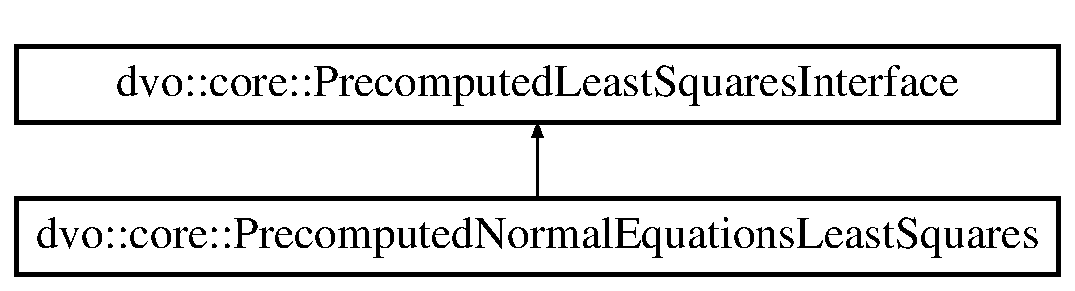
\includegraphics[height=2.000000cm]{classdvo_1_1core_1_1_precomputed_least_squares_interface}
\end{center}
\end{figure}
\subsection*{Public Member Functions}
\begin{DoxyCompactItemize}
\item 
virtual \mbox{\hyperlink{classdvo_1_1core_1_1_precomputed_least_squares_interface_ac9662bd4fa39b8acc2df291c7618953c}{$\sim$\+Precomputed\+Least\+Squares\+Interface}} ()
\item 
virtual void \mbox{\hyperlink{classdvo_1_1core_1_1_precomputed_least_squares_interface_abfd7276b663ea0afda8358a2ec9c96fe}{initialize}} (const size\+\_\+t maxnum\+\_\+constraints)=0
\item 
virtual void \mbox{\hyperlink{classdvo_1_1core_1_1_precomputed_least_squares_interface_a216ce9b1040fe23557e7ef22d4369dad}{add\+Constraint}} (const size\+\_\+t \&idx, const \mbox{\hyperlink{namespacedvo_1_1core_a05327f3312d32a301bce9fccda9e5807}{Vector6}} \&J)=0
\item 
virtual void \mbox{\hyperlink{classdvo_1_1core_1_1_precomputed_least_squares_interface_ae4b138a17c7959e780a0e30e935596e8}{reset}} ()=0
\item 
virtual void \mbox{\hyperlink{classdvo_1_1core_1_1_precomputed_least_squares_interface_a0ba3c8b938301387103912a9609a68dc}{next}} ()=0
\item 
virtual void \mbox{\hyperlink{classdvo_1_1core_1_1_precomputed_least_squares_interface_a9b879b6600b82a8b989770bf27dad7bc}{ignore\+Constraint}} (const size\+\_\+t \&idx)=0
\item 
virtual bool \mbox{\hyperlink{classdvo_1_1core_1_1_precomputed_least_squares_interface_a55870a4fa167484edf3e9b8120ad3232}{set\+Residual\+For\+Constraint}} (const size\+\_\+t \&idx, const \mbox{\hyperlink{namespacedvo_1_1core_ab9c199d221775a923e2549ad7e15c323}{Num\+Type}} \&res, const \mbox{\hyperlink{namespacedvo_1_1core_ab9c199d221775a923e2549ad7e15c323}{Num\+Type}} \&weight=1.\+0f)=0
\item 
virtual void \mbox{\hyperlink{classdvo_1_1core_1_1_precomputed_least_squares_interface_a6b811d85e3fe6a8a054b639171f9b353}{finish}} ()=0
\item 
virtual void \mbox{\hyperlink{classdvo_1_1core_1_1_precomputed_least_squares_interface_a036a293d0a53a7b019f8942776fb5d29}{solve}} (\mbox{\hyperlink{namespacedvo_1_1core_a05327f3312d32a301bce9fccda9e5807}{Vector6}} \&x)=0
\end{DoxyCompactItemize}


\subsection{Detailed Description}
Basic interface for algorithms solving 1 step of non-\/linear least squares where jacobians can be precomputed and don\textquotesingle{}t vary between iterations. 

\subsection{Constructor \& Destructor Documentation}
\mbox{\Hypertarget{classdvo_1_1core_1_1_precomputed_least_squares_interface_ac9662bd4fa39b8acc2df291c7618953c}\label{classdvo_1_1core_1_1_precomputed_least_squares_interface_ac9662bd4fa39b8acc2df291c7618953c}} 
\index{dvo\+::core\+::\+Precomputed\+Least\+Squares\+Interface@{dvo\+::core\+::\+Precomputed\+Least\+Squares\+Interface}!````~Precomputed\+Least\+Squares\+Interface@{$\sim$\+Precomputed\+Least\+Squares\+Interface}}
\index{````~Precomputed\+Least\+Squares\+Interface@{$\sim$\+Precomputed\+Least\+Squares\+Interface}!dvo\+::core\+::\+Precomputed\+Least\+Squares\+Interface@{dvo\+::core\+::\+Precomputed\+Least\+Squares\+Interface}}
\subsubsection{\texorpdfstring{$\sim$\+Precomputed\+Least\+Squares\+Interface()}{~PrecomputedLeastSquaresInterface()}}
{\footnotesize\ttfamily virtual dvo\+::core\+::\+Precomputed\+Least\+Squares\+Interface\+::$\sim$\+Precomputed\+Least\+Squares\+Interface (\begin{DoxyParamCaption}{ }\end{DoxyParamCaption})\hspace{0.3cm}{\ttfamily [inline]}, {\ttfamily [virtual]}}



\subsection{Member Function Documentation}
\mbox{\Hypertarget{classdvo_1_1core_1_1_precomputed_least_squares_interface_a216ce9b1040fe23557e7ef22d4369dad}\label{classdvo_1_1core_1_1_precomputed_least_squares_interface_a216ce9b1040fe23557e7ef22d4369dad}} 
\index{dvo\+::core\+::\+Precomputed\+Least\+Squares\+Interface@{dvo\+::core\+::\+Precomputed\+Least\+Squares\+Interface}!add\+Constraint@{add\+Constraint}}
\index{add\+Constraint@{add\+Constraint}!dvo\+::core\+::\+Precomputed\+Least\+Squares\+Interface@{dvo\+::core\+::\+Precomputed\+Least\+Squares\+Interface}}
\subsubsection{\texorpdfstring{add\+Constraint()}{addConstraint()}}
{\footnotesize\ttfamily virtual void dvo\+::core\+::\+Precomputed\+Least\+Squares\+Interface\+::add\+Constraint (\begin{DoxyParamCaption}\item[{const size\+\_\+t \&}]{idx,  }\item[{const \mbox{\hyperlink{namespacedvo_1_1core_a05327f3312d32a301bce9fccda9e5807}{Vector6}} \&}]{J }\end{DoxyParamCaption})\hspace{0.3cm}{\ttfamily [pure virtual]}}



Implemented in \mbox{\hyperlink{classdvo_1_1core_1_1_precomputed_normal_equations_least_squares_a8fda94e1f0b88e65f2f3c7e98597f662}{dvo\+::core\+::\+Precomputed\+Normal\+Equations\+Least\+Squares}}.

\mbox{\Hypertarget{classdvo_1_1core_1_1_precomputed_least_squares_interface_a6b811d85e3fe6a8a054b639171f9b353}\label{classdvo_1_1core_1_1_precomputed_least_squares_interface_a6b811d85e3fe6a8a054b639171f9b353}} 
\index{dvo\+::core\+::\+Precomputed\+Least\+Squares\+Interface@{dvo\+::core\+::\+Precomputed\+Least\+Squares\+Interface}!finish@{finish}}
\index{finish@{finish}!dvo\+::core\+::\+Precomputed\+Least\+Squares\+Interface@{dvo\+::core\+::\+Precomputed\+Least\+Squares\+Interface}}
\subsubsection{\texorpdfstring{finish()}{finish()}}
{\footnotesize\ttfamily virtual void dvo\+::core\+::\+Precomputed\+Least\+Squares\+Interface\+::finish (\begin{DoxyParamCaption}{ }\end{DoxyParamCaption})\hspace{0.3cm}{\ttfamily [pure virtual]}}



Implemented in \mbox{\hyperlink{classdvo_1_1core_1_1_precomputed_normal_equations_least_squares_a57b83cc3f829f4416b09d4334206a592}{dvo\+::core\+::\+Precomputed\+Normal\+Equations\+Least\+Squares}}.

\mbox{\Hypertarget{classdvo_1_1core_1_1_precomputed_least_squares_interface_a9b879b6600b82a8b989770bf27dad7bc}\label{classdvo_1_1core_1_1_precomputed_least_squares_interface_a9b879b6600b82a8b989770bf27dad7bc}} 
\index{dvo\+::core\+::\+Precomputed\+Least\+Squares\+Interface@{dvo\+::core\+::\+Precomputed\+Least\+Squares\+Interface}!ignore\+Constraint@{ignore\+Constraint}}
\index{ignore\+Constraint@{ignore\+Constraint}!dvo\+::core\+::\+Precomputed\+Least\+Squares\+Interface@{dvo\+::core\+::\+Precomputed\+Least\+Squares\+Interface}}
\subsubsection{\texorpdfstring{ignore\+Constraint()}{ignoreConstraint()}}
{\footnotesize\ttfamily virtual void dvo\+::core\+::\+Precomputed\+Least\+Squares\+Interface\+::ignore\+Constraint (\begin{DoxyParamCaption}\item[{const size\+\_\+t \&}]{idx }\end{DoxyParamCaption})\hspace{0.3cm}{\ttfamily [pure virtual]}}



Implemented in \mbox{\hyperlink{classdvo_1_1core_1_1_precomputed_normal_equations_least_squares_a3abc1c62317598bbbacf3b021d39bff3}{dvo\+::core\+::\+Precomputed\+Normal\+Equations\+Least\+Squares}}.

\mbox{\Hypertarget{classdvo_1_1core_1_1_precomputed_least_squares_interface_abfd7276b663ea0afda8358a2ec9c96fe}\label{classdvo_1_1core_1_1_precomputed_least_squares_interface_abfd7276b663ea0afda8358a2ec9c96fe}} 
\index{dvo\+::core\+::\+Precomputed\+Least\+Squares\+Interface@{dvo\+::core\+::\+Precomputed\+Least\+Squares\+Interface}!initialize@{initialize}}
\index{initialize@{initialize}!dvo\+::core\+::\+Precomputed\+Least\+Squares\+Interface@{dvo\+::core\+::\+Precomputed\+Least\+Squares\+Interface}}
\subsubsection{\texorpdfstring{initialize()}{initialize()}}
{\footnotesize\ttfamily virtual void dvo\+::core\+::\+Precomputed\+Least\+Squares\+Interface\+::initialize (\begin{DoxyParamCaption}\item[{const size\+\_\+t}]{maxnum\+\_\+constraints }\end{DoxyParamCaption})\hspace{0.3cm}{\ttfamily [pure virtual]}}



Implemented in \mbox{\hyperlink{classdvo_1_1core_1_1_precomputed_normal_equations_least_squares_a51e5717e0add36b37db3617d35c87c87}{dvo\+::core\+::\+Precomputed\+Normal\+Equations\+Least\+Squares}}.

\mbox{\Hypertarget{classdvo_1_1core_1_1_precomputed_least_squares_interface_a0ba3c8b938301387103912a9609a68dc}\label{classdvo_1_1core_1_1_precomputed_least_squares_interface_a0ba3c8b938301387103912a9609a68dc}} 
\index{dvo\+::core\+::\+Precomputed\+Least\+Squares\+Interface@{dvo\+::core\+::\+Precomputed\+Least\+Squares\+Interface}!next@{next}}
\index{next@{next}!dvo\+::core\+::\+Precomputed\+Least\+Squares\+Interface@{dvo\+::core\+::\+Precomputed\+Least\+Squares\+Interface}}
\subsubsection{\texorpdfstring{next()}{next()}}
{\footnotesize\ttfamily virtual void dvo\+::core\+::\+Precomputed\+Least\+Squares\+Interface\+::next (\begin{DoxyParamCaption}{ }\end{DoxyParamCaption})\hspace{0.3cm}{\ttfamily [pure virtual]}}



Implemented in \mbox{\hyperlink{classdvo_1_1core_1_1_precomputed_normal_equations_least_squares_a514bd37f6bbfeb8cb1788e6fdabc0e32}{dvo\+::core\+::\+Precomputed\+Normal\+Equations\+Least\+Squares}}.

\mbox{\Hypertarget{classdvo_1_1core_1_1_precomputed_least_squares_interface_ae4b138a17c7959e780a0e30e935596e8}\label{classdvo_1_1core_1_1_precomputed_least_squares_interface_ae4b138a17c7959e780a0e30e935596e8}} 
\index{dvo\+::core\+::\+Precomputed\+Least\+Squares\+Interface@{dvo\+::core\+::\+Precomputed\+Least\+Squares\+Interface}!reset@{reset}}
\index{reset@{reset}!dvo\+::core\+::\+Precomputed\+Least\+Squares\+Interface@{dvo\+::core\+::\+Precomputed\+Least\+Squares\+Interface}}
\subsubsection{\texorpdfstring{reset()}{reset()}}
{\footnotesize\ttfamily virtual void dvo\+::core\+::\+Precomputed\+Least\+Squares\+Interface\+::reset (\begin{DoxyParamCaption}{ }\end{DoxyParamCaption})\hspace{0.3cm}{\ttfamily [pure virtual]}}



Implemented in \mbox{\hyperlink{classdvo_1_1core_1_1_precomputed_normal_equations_least_squares_a591e3030f4736c580e37338ba747bc83}{dvo\+::core\+::\+Precomputed\+Normal\+Equations\+Least\+Squares}}.

\mbox{\Hypertarget{classdvo_1_1core_1_1_precomputed_least_squares_interface_a55870a4fa167484edf3e9b8120ad3232}\label{classdvo_1_1core_1_1_precomputed_least_squares_interface_a55870a4fa167484edf3e9b8120ad3232}} 
\index{dvo\+::core\+::\+Precomputed\+Least\+Squares\+Interface@{dvo\+::core\+::\+Precomputed\+Least\+Squares\+Interface}!set\+Residual\+For\+Constraint@{set\+Residual\+For\+Constraint}}
\index{set\+Residual\+For\+Constraint@{set\+Residual\+For\+Constraint}!dvo\+::core\+::\+Precomputed\+Least\+Squares\+Interface@{dvo\+::core\+::\+Precomputed\+Least\+Squares\+Interface}}
\subsubsection{\texorpdfstring{set\+Residual\+For\+Constraint()}{setResidualForConstraint()}}
{\footnotesize\ttfamily virtual bool dvo\+::core\+::\+Precomputed\+Least\+Squares\+Interface\+::set\+Residual\+For\+Constraint (\begin{DoxyParamCaption}\item[{const size\+\_\+t \&}]{idx,  }\item[{const \mbox{\hyperlink{namespacedvo_1_1core_ab9c199d221775a923e2549ad7e15c323}{Num\+Type}} \&}]{res,  }\item[{const \mbox{\hyperlink{namespacedvo_1_1core_ab9c199d221775a923e2549ad7e15c323}{Num\+Type}} \&}]{weight = {\ttfamily 1.0f} }\end{DoxyParamCaption})\hspace{0.3cm}{\ttfamily [pure virtual]}}



Implemented in \mbox{\hyperlink{classdvo_1_1core_1_1_precomputed_normal_equations_least_squares_a5eb65ee043d392def0ab917ec18cf6ef}{dvo\+::core\+::\+Precomputed\+Normal\+Equations\+Least\+Squares}}.

\mbox{\Hypertarget{classdvo_1_1core_1_1_precomputed_least_squares_interface_a036a293d0a53a7b019f8942776fb5d29}\label{classdvo_1_1core_1_1_precomputed_least_squares_interface_a036a293d0a53a7b019f8942776fb5d29}} 
\index{dvo\+::core\+::\+Precomputed\+Least\+Squares\+Interface@{dvo\+::core\+::\+Precomputed\+Least\+Squares\+Interface}!solve@{solve}}
\index{solve@{solve}!dvo\+::core\+::\+Precomputed\+Least\+Squares\+Interface@{dvo\+::core\+::\+Precomputed\+Least\+Squares\+Interface}}
\subsubsection{\texorpdfstring{solve()}{solve()}}
{\footnotesize\ttfamily virtual void dvo\+::core\+::\+Precomputed\+Least\+Squares\+Interface\+::solve (\begin{DoxyParamCaption}\item[{\mbox{\hyperlink{namespacedvo_1_1core_a05327f3312d32a301bce9fccda9e5807}{Vector6}} \&}]{x }\end{DoxyParamCaption})\hspace{0.3cm}{\ttfamily [pure virtual]}}



Implemented in \mbox{\hyperlink{classdvo_1_1core_1_1_precomputed_normal_equations_least_squares_a9749ed4314ae7ed7dbfa05c35a9e4a51}{dvo\+::core\+::\+Precomputed\+Normal\+Equations\+Least\+Squares}}.



The documentation for this class was generated from the following file\+:\begin{DoxyCompactItemize}
\item 
dvo\+\_\+core/include/dvo/core/\mbox{\hyperlink{least__squares_8h}{least\+\_\+squares.\+h}}\end{DoxyCompactItemize}

\hypertarget{classdvo_1_1core_1_1_precomputed_normal_equations_least_squares}{}\section{dvo\+:\+:core\+:\+:Precomputed\+Normal\+Equations\+Least\+Squares Class Reference}
\label{classdvo_1_1core_1_1_precomputed_normal_equations_least_squares}\index{dvo\+::core\+::\+Precomputed\+Normal\+Equations\+Least\+Squares@{dvo\+::core\+::\+Precomputed\+Normal\+Equations\+Least\+Squares}}


{\ttfamily \#include $<$least\+\_\+squares.\+h$>$}

Inheritance diagram for dvo\+:\+:core\+:\+:Precomputed\+Normal\+Equations\+Least\+Squares\+:\begin{figure}[H]
\begin{center}
\leavevmode
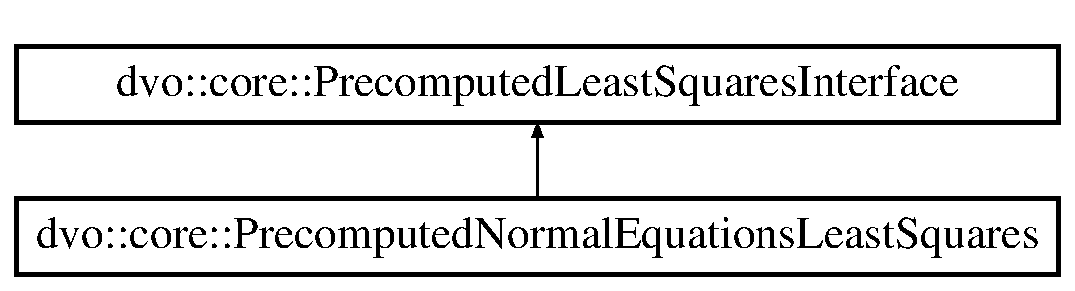
\includegraphics[height=2.000000cm]{classdvo_1_1core_1_1_precomputed_normal_equations_least_squares}
\end{center}
\end{figure}
\subsection*{Public Member Functions}
\begin{DoxyCompactItemize}
\item 
virtual \mbox{\hyperlink{classdvo_1_1core_1_1_precomputed_normal_equations_least_squares_aaadc7769e3857383066d302426d3cf3a}{$\sim$\+Precomputed\+Normal\+Equations\+Least\+Squares}} ()
\item 
virtual void \mbox{\hyperlink{classdvo_1_1core_1_1_precomputed_normal_equations_least_squares_a51e5717e0add36b37db3617d35c87c87}{initialize}} (const size\+\_\+t \mbox{\hyperlink{classdvo_1_1core_1_1_precomputed_normal_equations_least_squares_aac9bca6070c75a91e4c2777b137df9a2}{maxnum\+\_\+constraints}})
\item 
virtual void \mbox{\hyperlink{classdvo_1_1core_1_1_precomputed_normal_equations_least_squares_a8fda94e1f0b88e65f2f3c7e98597f662}{add\+Constraint}} (const size\+\_\+t \&idx, const \mbox{\hyperlink{namespacedvo_1_1core_a05327f3312d32a301bce9fccda9e5807}{Vector6}} \&J)
\item 
virtual void \mbox{\hyperlink{classdvo_1_1core_1_1_precomputed_normal_equations_least_squares_a591e3030f4736c580e37338ba747bc83}{reset}} ()
\item 
virtual void \mbox{\hyperlink{classdvo_1_1core_1_1_precomputed_normal_equations_least_squares_a514bd37f6bbfeb8cb1788e6fdabc0e32}{next}} ()
\item 
virtual void \mbox{\hyperlink{classdvo_1_1core_1_1_precomputed_normal_equations_least_squares_a3abc1c62317598bbbacf3b021d39bff3}{ignore\+Constraint}} (const size\+\_\+t \&idx)
\item 
virtual bool \mbox{\hyperlink{classdvo_1_1core_1_1_precomputed_normal_equations_least_squares_a5eb65ee043d392def0ab917ec18cf6ef}{set\+Residual\+For\+Constraint}} (const size\+\_\+t \&idx, const \mbox{\hyperlink{namespacedvo_1_1core_ab9c199d221775a923e2549ad7e15c323}{Num\+Type}} \&res, const \mbox{\hyperlink{namespacedvo_1_1core_ab9c199d221775a923e2549ad7e15c323}{Num\+Type}} \&weight=1.\+0f)
\item 
virtual void \mbox{\hyperlink{classdvo_1_1core_1_1_precomputed_normal_equations_least_squares_a57b83cc3f829f4416b09d4334206a592}{finish}} ()
\item 
virtual void \mbox{\hyperlink{classdvo_1_1core_1_1_precomputed_normal_equations_least_squares_a9749ed4314ae7ed7dbfa05c35a9e4a51}{solve}} (\mbox{\hyperlink{namespacedvo_1_1core_a05327f3312d32a301bce9fccda9e5807}{Vector6}} \&x)
\end{DoxyCompactItemize}
\subsection*{Public Attributes}
\begin{DoxyCompactItemize}
\item 
\mbox{\hyperlink{classdvo_1_1core_1_1_precomputed_normal_equations_least_squares_a5e379002dbbd2569ed4f0580eab97156}{E\+I\+G\+E\+N\+\_\+\+M\+A\+K\+E\+\_\+\+A\+L\+I\+G\+N\+E\+D\+\_\+\+O\+P\+E\+R\+A\+T\+O\+R\+\_\+\+N\+EW}}
\item 
\mbox{\hyperlink{namespacedvo_1_1core_a7b76cdc563f01ec2220fd58316004626}{Matrix6x6}} \mbox{\hyperlink{classdvo_1_1core_1_1_precomputed_normal_equations_least_squares_a95ecca09c734f950f5e6c03d2e1c5e76}{A}}
\item 
\mbox{\hyperlink{namespacedvo_1_1core_a05327f3312d32a301bce9fccda9e5807}{Vector6}} \mbox{\hyperlink{classdvo_1_1core_1_1_precomputed_normal_equations_least_squares_a81f932997bbc52fe2df57403e64fd6f6}{b}}
\item 
double \mbox{\hyperlink{classdvo_1_1core_1_1_precomputed_normal_equations_least_squares_ab466793175fcae83f158540f07e0cdb2}{error}}
\item 
size\+\_\+t \mbox{\hyperlink{classdvo_1_1core_1_1_precomputed_normal_equations_least_squares_aac9bca6070c75a91e4c2777b137df9a2}{maxnum\+\_\+constraints}}
\item 
size\+\_\+t \mbox{\hyperlink{classdvo_1_1core_1_1_precomputed_normal_equations_least_squares_a1895a0916656b67cdc410d627f779a94}{num\+\_\+constraints}}
\item 
const uchar $\ast$ \mbox{\hyperlink{classdvo_1_1core_1_1_precomputed_normal_equations_least_squares_a06ee504a39a8ebf770bcec527e22fd34}{mask\+\_\+ptr\+\_\+}}
\end{DoxyCompactItemize}


\subsection{Detailed Description}
Builds normal equations and solves them with Cholesky decomposition. 

\subsection{Constructor \& Destructor Documentation}
\mbox{\Hypertarget{classdvo_1_1core_1_1_precomputed_normal_equations_least_squares_aaadc7769e3857383066d302426d3cf3a}\label{classdvo_1_1core_1_1_precomputed_normal_equations_least_squares_aaadc7769e3857383066d302426d3cf3a}} 
\index{dvo\+::core\+::\+Precomputed\+Normal\+Equations\+Least\+Squares@{dvo\+::core\+::\+Precomputed\+Normal\+Equations\+Least\+Squares}!````~Precomputed\+Normal\+Equations\+Least\+Squares@{$\sim$\+Precomputed\+Normal\+Equations\+Least\+Squares}}
\index{````~Precomputed\+Normal\+Equations\+Least\+Squares@{$\sim$\+Precomputed\+Normal\+Equations\+Least\+Squares}!dvo\+::core\+::\+Precomputed\+Normal\+Equations\+Least\+Squares@{dvo\+::core\+::\+Precomputed\+Normal\+Equations\+Least\+Squares}}
\subsubsection{\texorpdfstring{$\sim$\+Precomputed\+Normal\+Equations\+Least\+Squares()}{~PrecomputedNormalEquationsLeastSquares()}}
{\footnotesize\ttfamily dvo\+::core\+::\+Precomputed\+Normal\+Equations\+Least\+Squares\+::$\sim$\+Precomputed\+Normal\+Equations\+Least\+Squares (\begin{DoxyParamCaption}{ }\end{DoxyParamCaption})\hspace{0.3cm}{\ttfamily [virtual]}}



\subsection{Member Function Documentation}
\mbox{\Hypertarget{classdvo_1_1core_1_1_precomputed_normal_equations_least_squares_a8fda94e1f0b88e65f2f3c7e98597f662}\label{classdvo_1_1core_1_1_precomputed_normal_equations_least_squares_a8fda94e1f0b88e65f2f3c7e98597f662}} 
\index{dvo\+::core\+::\+Precomputed\+Normal\+Equations\+Least\+Squares@{dvo\+::core\+::\+Precomputed\+Normal\+Equations\+Least\+Squares}!add\+Constraint@{add\+Constraint}}
\index{add\+Constraint@{add\+Constraint}!dvo\+::core\+::\+Precomputed\+Normal\+Equations\+Least\+Squares@{dvo\+::core\+::\+Precomputed\+Normal\+Equations\+Least\+Squares}}
\subsubsection{\texorpdfstring{add\+Constraint()}{addConstraint()}}
{\footnotesize\ttfamily void dvo\+::core\+::\+Precomputed\+Normal\+Equations\+Least\+Squares\+::add\+Constraint (\begin{DoxyParamCaption}\item[{const size\+\_\+t \&}]{idx,  }\item[{const \mbox{\hyperlink{namespacedvo_1_1core_a05327f3312d32a301bce9fccda9e5807}{Vector6}} \&}]{J }\end{DoxyParamCaption})\hspace{0.3cm}{\ttfamily [virtual]}}



Implements \mbox{\hyperlink{classdvo_1_1core_1_1_precomputed_least_squares_interface_a216ce9b1040fe23557e7ef22d4369dad}{dvo\+::core\+::\+Precomputed\+Least\+Squares\+Interface}}.

\mbox{\Hypertarget{classdvo_1_1core_1_1_precomputed_normal_equations_least_squares_a57b83cc3f829f4416b09d4334206a592}\label{classdvo_1_1core_1_1_precomputed_normal_equations_least_squares_a57b83cc3f829f4416b09d4334206a592}} 
\index{dvo\+::core\+::\+Precomputed\+Normal\+Equations\+Least\+Squares@{dvo\+::core\+::\+Precomputed\+Normal\+Equations\+Least\+Squares}!finish@{finish}}
\index{finish@{finish}!dvo\+::core\+::\+Precomputed\+Normal\+Equations\+Least\+Squares@{dvo\+::core\+::\+Precomputed\+Normal\+Equations\+Least\+Squares}}
\subsubsection{\texorpdfstring{finish()}{finish()}}
{\footnotesize\ttfamily void dvo\+::core\+::\+Precomputed\+Normal\+Equations\+Least\+Squares\+::finish (\begin{DoxyParamCaption}{ }\end{DoxyParamCaption})\hspace{0.3cm}{\ttfamily [virtual]}}



Implements \mbox{\hyperlink{classdvo_1_1core_1_1_precomputed_least_squares_interface_a6b811d85e3fe6a8a054b639171f9b353}{dvo\+::core\+::\+Precomputed\+Least\+Squares\+Interface}}.

\mbox{\Hypertarget{classdvo_1_1core_1_1_precomputed_normal_equations_least_squares_a3abc1c62317598bbbacf3b021d39bff3}\label{classdvo_1_1core_1_1_precomputed_normal_equations_least_squares_a3abc1c62317598bbbacf3b021d39bff3}} 
\index{dvo\+::core\+::\+Precomputed\+Normal\+Equations\+Least\+Squares@{dvo\+::core\+::\+Precomputed\+Normal\+Equations\+Least\+Squares}!ignore\+Constraint@{ignore\+Constraint}}
\index{ignore\+Constraint@{ignore\+Constraint}!dvo\+::core\+::\+Precomputed\+Normal\+Equations\+Least\+Squares@{dvo\+::core\+::\+Precomputed\+Normal\+Equations\+Least\+Squares}}
\subsubsection{\texorpdfstring{ignore\+Constraint()}{ignoreConstraint()}}
{\footnotesize\ttfamily void dvo\+::core\+::\+Precomputed\+Normal\+Equations\+Least\+Squares\+::ignore\+Constraint (\begin{DoxyParamCaption}\item[{const size\+\_\+t \&}]{idx }\end{DoxyParamCaption})\hspace{0.3cm}{\ttfamily [virtual]}}

J is already multiplied with normalizer, so it is\+:

J\textquotesingle{} $\ast$ J\textquotesingle{}.transpose() $\ast$ normalizer $\ast$ normalizer

multiplying with normalizer\+\_\+inverse gives\+:

J\textquotesingle{} $\ast$ J\textquotesingle{}.transpose() $\ast$ normalizer $\ast$ normalizer $\ast$ normalizer\+\_\+inverse

resulting in\+:

J\textquotesingle{} $\ast$ J\textquotesingle{}.transpose() $\ast$ normalizer

Implements \mbox{\hyperlink{classdvo_1_1core_1_1_precomputed_least_squares_interface_a9b879b6600b82a8b989770bf27dad7bc}{dvo\+::core\+::\+Precomputed\+Least\+Squares\+Interface}}.

\mbox{\Hypertarget{classdvo_1_1core_1_1_precomputed_normal_equations_least_squares_a51e5717e0add36b37db3617d35c87c87}\label{classdvo_1_1core_1_1_precomputed_normal_equations_least_squares_a51e5717e0add36b37db3617d35c87c87}} 
\index{dvo\+::core\+::\+Precomputed\+Normal\+Equations\+Least\+Squares@{dvo\+::core\+::\+Precomputed\+Normal\+Equations\+Least\+Squares}!initialize@{initialize}}
\index{initialize@{initialize}!dvo\+::core\+::\+Precomputed\+Normal\+Equations\+Least\+Squares@{dvo\+::core\+::\+Precomputed\+Normal\+Equations\+Least\+Squares}}
\subsubsection{\texorpdfstring{initialize()}{initialize()}}
{\footnotesize\ttfamily void dvo\+::core\+::\+Precomputed\+Normal\+Equations\+Least\+Squares\+::initialize (\begin{DoxyParamCaption}\item[{const size\+\_\+t}]{maxnum\+\_\+constraints }\end{DoxyParamCaption})\hspace{0.3cm}{\ttfamily [virtual]}}



Implements \mbox{\hyperlink{classdvo_1_1core_1_1_precomputed_least_squares_interface_abfd7276b663ea0afda8358a2ec9c96fe}{dvo\+::core\+::\+Precomputed\+Least\+Squares\+Interface}}.

\mbox{\Hypertarget{classdvo_1_1core_1_1_precomputed_normal_equations_least_squares_a514bd37f6bbfeb8cb1788e6fdabc0e32}\label{classdvo_1_1core_1_1_precomputed_normal_equations_least_squares_a514bd37f6bbfeb8cb1788e6fdabc0e32}} 
\index{dvo\+::core\+::\+Precomputed\+Normal\+Equations\+Least\+Squares@{dvo\+::core\+::\+Precomputed\+Normal\+Equations\+Least\+Squares}!next@{next}}
\index{next@{next}!dvo\+::core\+::\+Precomputed\+Normal\+Equations\+Least\+Squares@{dvo\+::core\+::\+Precomputed\+Normal\+Equations\+Least\+Squares}}
\subsubsection{\texorpdfstring{next()}{next()}}
{\footnotesize\ttfamily void dvo\+::core\+::\+Precomputed\+Normal\+Equations\+Least\+Squares\+::next (\begin{DoxyParamCaption}{ }\end{DoxyParamCaption})\hspace{0.3cm}{\ttfamily [virtual]}}



Implements \mbox{\hyperlink{classdvo_1_1core_1_1_precomputed_least_squares_interface_a0ba3c8b938301387103912a9609a68dc}{dvo\+::core\+::\+Precomputed\+Least\+Squares\+Interface}}.

\mbox{\Hypertarget{classdvo_1_1core_1_1_precomputed_normal_equations_least_squares_a591e3030f4736c580e37338ba747bc83}\label{classdvo_1_1core_1_1_precomputed_normal_equations_least_squares_a591e3030f4736c580e37338ba747bc83}} 
\index{dvo\+::core\+::\+Precomputed\+Normal\+Equations\+Least\+Squares@{dvo\+::core\+::\+Precomputed\+Normal\+Equations\+Least\+Squares}!reset@{reset}}
\index{reset@{reset}!dvo\+::core\+::\+Precomputed\+Normal\+Equations\+Least\+Squares@{dvo\+::core\+::\+Precomputed\+Normal\+Equations\+Least\+Squares}}
\subsubsection{\texorpdfstring{reset()}{reset()}}
{\footnotesize\ttfamily void dvo\+::core\+::\+Precomputed\+Normal\+Equations\+Least\+Squares\+::reset (\begin{DoxyParamCaption}{ }\end{DoxyParamCaption})\hspace{0.3cm}{\ttfamily [virtual]}}



Implements \mbox{\hyperlink{classdvo_1_1core_1_1_precomputed_least_squares_interface_ae4b138a17c7959e780a0e30e935596e8}{dvo\+::core\+::\+Precomputed\+Least\+Squares\+Interface}}.

\mbox{\Hypertarget{classdvo_1_1core_1_1_precomputed_normal_equations_least_squares_a5eb65ee043d392def0ab917ec18cf6ef}\label{classdvo_1_1core_1_1_precomputed_normal_equations_least_squares_a5eb65ee043d392def0ab917ec18cf6ef}} 
\index{dvo\+::core\+::\+Precomputed\+Normal\+Equations\+Least\+Squares@{dvo\+::core\+::\+Precomputed\+Normal\+Equations\+Least\+Squares}!set\+Residual\+For\+Constraint@{set\+Residual\+For\+Constraint}}
\index{set\+Residual\+For\+Constraint@{set\+Residual\+For\+Constraint}!dvo\+::core\+::\+Precomputed\+Normal\+Equations\+Least\+Squares@{dvo\+::core\+::\+Precomputed\+Normal\+Equations\+Least\+Squares}}
\subsubsection{\texorpdfstring{set\+Residual\+For\+Constraint()}{setResidualForConstraint()}}
{\footnotesize\ttfamily bool dvo\+::core\+::\+Precomputed\+Normal\+Equations\+Least\+Squares\+::set\+Residual\+For\+Constraint (\begin{DoxyParamCaption}\item[{const size\+\_\+t \&}]{idx,  }\item[{const \mbox{\hyperlink{namespacedvo_1_1core_ab9c199d221775a923e2549ad7e15c323}{Num\+Type}} \&}]{res,  }\item[{const \mbox{\hyperlink{namespacedvo_1_1core_ab9c199d221775a923e2549ad7e15c323}{Num\+Type}} \&}]{weight = {\ttfamily 1.0f} }\end{DoxyParamCaption})\hspace{0.3cm}{\ttfamily [virtual]}}



Implements \mbox{\hyperlink{classdvo_1_1core_1_1_precomputed_least_squares_interface_a55870a4fa167484edf3e9b8120ad3232}{dvo\+::core\+::\+Precomputed\+Least\+Squares\+Interface}}.

\mbox{\Hypertarget{classdvo_1_1core_1_1_precomputed_normal_equations_least_squares_a9749ed4314ae7ed7dbfa05c35a9e4a51}\label{classdvo_1_1core_1_1_precomputed_normal_equations_least_squares_a9749ed4314ae7ed7dbfa05c35a9e4a51}} 
\index{dvo\+::core\+::\+Precomputed\+Normal\+Equations\+Least\+Squares@{dvo\+::core\+::\+Precomputed\+Normal\+Equations\+Least\+Squares}!solve@{solve}}
\index{solve@{solve}!dvo\+::core\+::\+Precomputed\+Normal\+Equations\+Least\+Squares@{dvo\+::core\+::\+Precomputed\+Normal\+Equations\+Least\+Squares}}
\subsubsection{\texorpdfstring{solve()}{solve()}}
{\footnotesize\ttfamily void dvo\+::core\+::\+Precomputed\+Normal\+Equations\+Least\+Squares\+::solve (\begin{DoxyParamCaption}\item[{\mbox{\hyperlink{namespacedvo_1_1core_a05327f3312d32a301bce9fccda9e5807}{Vector6}} \&}]{x }\end{DoxyParamCaption})\hspace{0.3cm}{\ttfamily [virtual]}}



Implements \mbox{\hyperlink{classdvo_1_1core_1_1_precomputed_least_squares_interface_a036a293d0a53a7b019f8942776fb5d29}{dvo\+::core\+::\+Precomputed\+Least\+Squares\+Interface}}.



\subsection{Member Data Documentation}
\mbox{\Hypertarget{classdvo_1_1core_1_1_precomputed_normal_equations_least_squares_a95ecca09c734f950f5e6c03d2e1c5e76}\label{classdvo_1_1core_1_1_precomputed_normal_equations_least_squares_a95ecca09c734f950f5e6c03d2e1c5e76}} 
\index{dvo\+::core\+::\+Precomputed\+Normal\+Equations\+Least\+Squares@{dvo\+::core\+::\+Precomputed\+Normal\+Equations\+Least\+Squares}!A@{A}}
\index{A@{A}!dvo\+::core\+::\+Precomputed\+Normal\+Equations\+Least\+Squares@{dvo\+::core\+::\+Precomputed\+Normal\+Equations\+Least\+Squares}}
\subsubsection{\texorpdfstring{A}{A}}
{\footnotesize\ttfamily \mbox{\hyperlink{namespacedvo_1_1core_a7b76cdc563f01ec2220fd58316004626}{Matrix6x6}} dvo\+::core\+::\+Precomputed\+Normal\+Equations\+Least\+Squares\+::A}

\mbox{\Hypertarget{classdvo_1_1core_1_1_precomputed_normal_equations_least_squares_a81f932997bbc52fe2df57403e64fd6f6}\label{classdvo_1_1core_1_1_precomputed_normal_equations_least_squares_a81f932997bbc52fe2df57403e64fd6f6}} 
\index{dvo\+::core\+::\+Precomputed\+Normal\+Equations\+Least\+Squares@{dvo\+::core\+::\+Precomputed\+Normal\+Equations\+Least\+Squares}!b@{b}}
\index{b@{b}!dvo\+::core\+::\+Precomputed\+Normal\+Equations\+Least\+Squares@{dvo\+::core\+::\+Precomputed\+Normal\+Equations\+Least\+Squares}}
\subsubsection{\texorpdfstring{b}{b}}
{\footnotesize\ttfamily \mbox{\hyperlink{namespacedvo_1_1core_a05327f3312d32a301bce9fccda9e5807}{Vector6}} dvo\+::core\+::\+Precomputed\+Normal\+Equations\+Least\+Squares\+::b}

\mbox{\Hypertarget{classdvo_1_1core_1_1_precomputed_normal_equations_least_squares_a5e379002dbbd2569ed4f0580eab97156}\label{classdvo_1_1core_1_1_precomputed_normal_equations_least_squares_a5e379002dbbd2569ed4f0580eab97156}} 
\index{dvo\+::core\+::\+Precomputed\+Normal\+Equations\+Least\+Squares@{dvo\+::core\+::\+Precomputed\+Normal\+Equations\+Least\+Squares}!E\+I\+G\+E\+N\+\_\+\+M\+A\+K\+E\+\_\+\+A\+L\+I\+G\+N\+E\+D\+\_\+\+O\+P\+E\+R\+A\+T\+O\+R\+\_\+\+N\+EW@{E\+I\+G\+E\+N\+\_\+\+M\+A\+K\+E\+\_\+\+A\+L\+I\+G\+N\+E\+D\+\_\+\+O\+P\+E\+R\+A\+T\+O\+R\+\_\+\+N\+EW}}
\index{E\+I\+G\+E\+N\+\_\+\+M\+A\+K\+E\+\_\+\+A\+L\+I\+G\+N\+E\+D\+\_\+\+O\+P\+E\+R\+A\+T\+O\+R\+\_\+\+N\+EW@{E\+I\+G\+E\+N\+\_\+\+M\+A\+K\+E\+\_\+\+A\+L\+I\+G\+N\+E\+D\+\_\+\+O\+P\+E\+R\+A\+T\+O\+R\+\_\+\+N\+EW}!dvo\+::core\+::\+Precomputed\+Normal\+Equations\+Least\+Squares@{dvo\+::core\+::\+Precomputed\+Normal\+Equations\+Least\+Squares}}
\subsubsection{\texorpdfstring{E\+I\+G\+E\+N\+\_\+\+M\+A\+K\+E\+\_\+\+A\+L\+I\+G\+N\+E\+D\+\_\+\+O\+P\+E\+R\+A\+T\+O\+R\+\_\+\+N\+EW}{EIGEN\_MAKE\_ALIGNED\_OPERATOR\_NEW}}
{\footnotesize\ttfamily dvo\+::core\+::\+Precomputed\+Normal\+Equations\+Least\+Squares\+::\+E\+I\+G\+E\+N\+\_\+\+M\+A\+K\+E\+\_\+\+A\+L\+I\+G\+N\+E\+D\+\_\+\+O\+P\+E\+R\+A\+T\+O\+R\+\_\+\+N\+EW}

\mbox{\Hypertarget{classdvo_1_1core_1_1_precomputed_normal_equations_least_squares_ab466793175fcae83f158540f07e0cdb2}\label{classdvo_1_1core_1_1_precomputed_normal_equations_least_squares_ab466793175fcae83f158540f07e0cdb2}} 
\index{dvo\+::core\+::\+Precomputed\+Normal\+Equations\+Least\+Squares@{dvo\+::core\+::\+Precomputed\+Normal\+Equations\+Least\+Squares}!error@{error}}
\index{error@{error}!dvo\+::core\+::\+Precomputed\+Normal\+Equations\+Least\+Squares@{dvo\+::core\+::\+Precomputed\+Normal\+Equations\+Least\+Squares}}
\subsubsection{\texorpdfstring{error}{error}}
{\footnotesize\ttfamily double dvo\+::core\+::\+Precomputed\+Normal\+Equations\+Least\+Squares\+::error}

\mbox{\Hypertarget{classdvo_1_1core_1_1_precomputed_normal_equations_least_squares_a06ee504a39a8ebf770bcec527e22fd34}\label{classdvo_1_1core_1_1_precomputed_normal_equations_least_squares_a06ee504a39a8ebf770bcec527e22fd34}} 
\index{dvo\+::core\+::\+Precomputed\+Normal\+Equations\+Least\+Squares@{dvo\+::core\+::\+Precomputed\+Normal\+Equations\+Least\+Squares}!mask\+\_\+ptr\+\_\+@{mask\+\_\+ptr\+\_\+}}
\index{mask\+\_\+ptr\+\_\+@{mask\+\_\+ptr\+\_\+}!dvo\+::core\+::\+Precomputed\+Normal\+Equations\+Least\+Squares@{dvo\+::core\+::\+Precomputed\+Normal\+Equations\+Least\+Squares}}
\subsubsection{\texorpdfstring{mask\+\_\+ptr\+\_\+}{mask\_ptr\_}}
{\footnotesize\ttfamily const uchar$\ast$ dvo\+::core\+::\+Precomputed\+Normal\+Equations\+Least\+Squares\+::mask\+\_\+ptr\+\_\+}

\mbox{\Hypertarget{classdvo_1_1core_1_1_precomputed_normal_equations_least_squares_aac9bca6070c75a91e4c2777b137df9a2}\label{classdvo_1_1core_1_1_precomputed_normal_equations_least_squares_aac9bca6070c75a91e4c2777b137df9a2}} 
\index{dvo\+::core\+::\+Precomputed\+Normal\+Equations\+Least\+Squares@{dvo\+::core\+::\+Precomputed\+Normal\+Equations\+Least\+Squares}!maxnum\+\_\+constraints@{maxnum\+\_\+constraints}}
\index{maxnum\+\_\+constraints@{maxnum\+\_\+constraints}!dvo\+::core\+::\+Precomputed\+Normal\+Equations\+Least\+Squares@{dvo\+::core\+::\+Precomputed\+Normal\+Equations\+Least\+Squares}}
\subsubsection{\texorpdfstring{maxnum\+\_\+constraints}{maxnum\_constraints}}
{\footnotesize\ttfamily size\+\_\+t dvo\+::core\+::\+Precomputed\+Normal\+Equations\+Least\+Squares\+::maxnum\+\_\+constraints}

\mbox{\Hypertarget{classdvo_1_1core_1_1_precomputed_normal_equations_least_squares_a1895a0916656b67cdc410d627f779a94}\label{classdvo_1_1core_1_1_precomputed_normal_equations_least_squares_a1895a0916656b67cdc410d627f779a94}} 
\index{dvo\+::core\+::\+Precomputed\+Normal\+Equations\+Least\+Squares@{dvo\+::core\+::\+Precomputed\+Normal\+Equations\+Least\+Squares}!num\+\_\+constraints@{num\+\_\+constraints}}
\index{num\+\_\+constraints@{num\+\_\+constraints}!dvo\+::core\+::\+Precomputed\+Normal\+Equations\+Least\+Squares@{dvo\+::core\+::\+Precomputed\+Normal\+Equations\+Least\+Squares}}
\subsubsection{\texorpdfstring{num\+\_\+constraints}{num\_constraints}}
{\footnotesize\ttfamily size\+\_\+t dvo\+::core\+::\+Precomputed\+Normal\+Equations\+Least\+Squares\+::num\+\_\+constraints}



The documentation for this class was generated from the following files\+:\begin{DoxyCompactItemize}
\item 
dvo\+\_\+core/include/dvo/core/\mbox{\hyperlink{least__squares_8h}{least\+\_\+squares.\+h}}\item 
dvo\+\_\+core/src/core/\mbox{\hyperlink{least__squares_8cpp}{least\+\_\+squares.\+cpp}}\end{DoxyCompactItemize}

\hypertarget{classdvo_1_1util_1_1_revertable}{}\section{dvo\+:\+:util\+:\+:Revertable$<$ T $>$ Class Template Reference}
\label{classdvo_1_1util_1_1_revertable}\index{dvo\+::util\+::\+Revertable$<$ T $>$@{dvo\+::util\+::\+Revertable$<$ T $>$}}


{\ttfamily \#include $<$revertable.\+h$>$}

\subsection*{Public Member Functions}
\begin{DoxyCompactItemize}
\item 
\mbox{\hyperlink{classdvo_1_1util_1_1_revertable_a5b791252e99ca8dab9a682a1b4981dd0}{Revertable}} (const T \&value)
\item 
const T \& \mbox{\hyperlink{classdvo_1_1util_1_1_revertable_ae583fea5c2d9f3e248f8f1d7bcdfd3d3}{operator()}} () const
\item 
T \& \mbox{\hyperlink{classdvo_1_1util_1_1_revertable_a09344cd96395e5e63ab57d33dbab55cf}{update}} ()
\item 
void \mbox{\hyperlink{classdvo_1_1util_1_1_revertable_ac4130b746441cb5d449d0ae24f6889f3}{revert}} ()
\end{DoxyCompactItemize}


\subsection{Constructor \& Destructor Documentation}
\mbox{\Hypertarget{classdvo_1_1util_1_1_revertable_a5b791252e99ca8dab9a682a1b4981dd0}\label{classdvo_1_1util_1_1_revertable_a5b791252e99ca8dab9a682a1b4981dd0}} 
\index{dvo\+::util\+::\+Revertable@{dvo\+::util\+::\+Revertable}!Revertable@{Revertable}}
\index{Revertable@{Revertable}!dvo\+::util\+::\+Revertable@{dvo\+::util\+::\+Revertable}}
\subsubsection{\texorpdfstring{Revertable()}{Revertable()}}
{\footnotesize\ttfamily template$<$typename T $>$ \\
\mbox{\hyperlink{classdvo_1_1util_1_1_revertable}{dvo\+::util\+::\+Revertable}}$<$ T $>$\+::\mbox{\hyperlink{classdvo_1_1util_1_1_revertable}{Revertable}} (\begin{DoxyParamCaption}\item[{const T \&}]{value }\end{DoxyParamCaption})\hspace{0.3cm}{\ttfamily [inline]}}



\subsection{Member Function Documentation}
\mbox{\Hypertarget{classdvo_1_1util_1_1_revertable_ae583fea5c2d9f3e248f8f1d7bcdfd3d3}\label{classdvo_1_1util_1_1_revertable_ae583fea5c2d9f3e248f8f1d7bcdfd3d3}} 
\index{dvo\+::util\+::\+Revertable@{dvo\+::util\+::\+Revertable}!operator()@{operator()}}
\index{operator()@{operator()}!dvo\+::util\+::\+Revertable@{dvo\+::util\+::\+Revertable}}
\subsubsection{\texorpdfstring{operator()()}{operator()()}}
{\footnotesize\ttfamily template$<$typename T $>$ \\
const T\& \mbox{\hyperlink{classdvo_1_1util_1_1_revertable}{dvo\+::util\+::\+Revertable}}$<$ T $>$\+::operator() (\begin{DoxyParamCaption}{ }\end{DoxyParamCaption}) const\hspace{0.3cm}{\ttfamily [inline]}}

\mbox{\Hypertarget{classdvo_1_1util_1_1_revertable_ac4130b746441cb5d449d0ae24f6889f3}\label{classdvo_1_1util_1_1_revertable_ac4130b746441cb5d449d0ae24f6889f3}} 
\index{dvo\+::util\+::\+Revertable@{dvo\+::util\+::\+Revertable}!revert@{revert}}
\index{revert@{revert}!dvo\+::util\+::\+Revertable@{dvo\+::util\+::\+Revertable}}
\subsubsection{\texorpdfstring{revert()}{revert()}}
{\footnotesize\ttfamily template$<$typename T $>$ \\
void \mbox{\hyperlink{classdvo_1_1util_1_1_revertable}{dvo\+::util\+::\+Revertable}}$<$ T $>$\+::revert (\begin{DoxyParamCaption}{ }\end{DoxyParamCaption})\hspace{0.3cm}{\ttfamily [inline]}}

\mbox{\Hypertarget{classdvo_1_1util_1_1_revertable_a09344cd96395e5e63ab57d33dbab55cf}\label{classdvo_1_1util_1_1_revertable_a09344cd96395e5e63ab57d33dbab55cf}} 
\index{dvo\+::util\+::\+Revertable@{dvo\+::util\+::\+Revertable}!update@{update}}
\index{update@{update}!dvo\+::util\+::\+Revertable@{dvo\+::util\+::\+Revertable}}
\subsubsection{\texorpdfstring{update()}{update()}}
{\footnotesize\ttfamily template$<$typename T $>$ \\
T\& \mbox{\hyperlink{classdvo_1_1util_1_1_revertable}{dvo\+::util\+::\+Revertable}}$<$ T $>$\+::update (\begin{DoxyParamCaption}{ }\end{DoxyParamCaption})\hspace{0.3cm}{\ttfamily [inline]}}



The documentation for this class was generated from the following file\+:\begin{DoxyCompactItemize}
\item 
dvo\+\_\+core/include/dvo/util/\mbox{\hyperlink{revertable_8h}{revertable.\+h}}\end{DoxyCompactItemize}

\hypertarget{structdvo_1_1core_1_1_rgbd_image}{}\section{dvo\+:\+:core\+:\+:Rgbd\+Image Struct Reference}
\label{structdvo_1_1core_1_1_rgbd_image}\index{dvo\+::core\+::\+Rgbd\+Image@{dvo\+::core\+::\+Rgbd\+Image}}


{\ttfamily \#include $<$rgbd\+\_\+image.\+h$>$}

\subsection*{Public Types}
\begin{DoxyCompactItemize}
\item 
typedef Eigen\+::\+Matrix$<$ float, 4, Eigen\+::\+Dynamic, Eigen\+::\+Col\+Major $>$ \mbox{\hyperlink{structdvo_1_1core_1_1_rgbd_image_a56820965eb98427d06e6733fe333cdc5}{Point\+Cloud}}
\end{DoxyCompactItemize}
\subsection*{Public Member Functions}
\begin{DoxyCompactItemize}
\item 
bool \mbox{\hyperlink{structdvo_1_1core_1_1_rgbd_image_aedc1a49823b9cc5afe16ace4b682fdb8}{has\+Intensity}} () const
\item 
bool \mbox{\hyperlink{structdvo_1_1core_1_1_rgbd_image_af939012f350c641cce1a7dc19c6a5967}{has\+Depth}} () const
\item 
bool \mbox{\hyperlink{structdvo_1_1core_1_1_rgbd_image_a9971d723c09f5eab20f5487993eb6b71}{has\+Rgb}} () const
\item 
void \mbox{\hyperlink{structdvo_1_1core_1_1_rgbd_image_ae75d152196893d0a8e7ca64f9142da82}{initialize}} ()
\item 
void \mbox{\hyperlink{structdvo_1_1core_1_1_rgbd_image_a7e92fbbf098e63f7eb9263775b99d606}{calculate\+Derivatives}} ()
\item 
bool \mbox{\hyperlink{structdvo_1_1core_1_1_rgbd_image_a66f7d5b2cd026ac8ec0b2e6a131f7aa6}{calculate\+Intensity\+Derivatives}} ()
\item 
void \mbox{\hyperlink{structdvo_1_1core_1_1_rgbd_image_aeca20a5666f5c9a532451e969d94e7bc}{calculate\+Depth\+Derivatives}} ()
\item 
void \mbox{\hyperlink{structdvo_1_1core_1_1_rgbd_image_ac034e5b79b4f39525d9a1eab1f98ec70}{build\+Point\+Cloud}} (const \mbox{\hyperlink{structdvo_1_1core_1_1_intrinsic_matrix}{Intrinsic\+Matrix}} \&intrinsics)
\item 
void \mbox{\hyperlink{structdvo_1_1core_1_1_rgbd_image_a9f476f47d4970842c7e9f96f6ad1c7a3}{warp\+Intensity}} (const \mbox{\hyperlink{namespacedvo_1_1core_af89a8f837f3ae51ed196b7988e59e53d}{Affine\+Transform}} \&transformation, const \mbox{\hyperlink{structdvo_1_1core_1_1_rgbd_image_a56820965eb98427d06e6733fe333cdc5}{Point\+Cloud}} \&reference\+\_\+pointcloud, const \mbox{\hyperlink{structdvo_1_1core_1_1_intrinsic_matrix}{Intrinsic\+Matrix}} \&intrinsics, \mbox{\hyperlink{structdvo_1_1core_1_1_rgbd_image}{Rgbd\+Image}} \&result, \mbox{\hyperlink{structdvo_1_1core_1_1_rgbd_image_a56820965eb98427d06e6733fe333cdc5}{Point\+Cloud}} \&transformed\+\_\+pointcloud)
\item 
void \mbox{\hyperlink{structdvo_1_1core_1_1_rgbd_image_a055ec4d22938a6deb2b2fabfe083aca3}{warp\+Intensity\+Sse}} (const \mbox{\hyperlink{namespacedvo_1_1core_af89a8f837f3ae51ed196b7988e59e53d}{Affine\+Transform}} \&transformation, const \mbox{\hyperlink{structdvo_1_1core_1_1_rgbd_image_a56820965eb98427d06e6733fe333cdc5}{Point\+Cloud}} \&reference\+\_\+pointcloud, const \mbox{\hyperlink{structdvo_1_1core_1_1_intrinsic_matrix}{Intrinsic\+Matrix}} \&intrinsics, \mbox{\hyperlink{structdvo_1_1core_1_1_rgbd_image}{Rgbd\+Image}} \&result, \mbox{\hyperlink{structdvo_1_1core_1_1_rgbd_image_a56820965eb98427d06e6733fe333cdc5}{Point\+Cloud}} \&transformed\+\_\+pointcloud)
\item 
void \mbox{\hyperlink{structdvo_1_1core_1_1_rgbd_image_af35a385488bc48bf81ebb5cb96f58449}{warp\+Intensity\+Sse}} (const \mbox{\hyperlink{namespacedvo_1_1core_af89a8f837f3ae51ed196b7988e59e53d}{Affine\+Transform}} \&transformation, const \mbox{\hyperlink{structdvo_1_1core_1_1_rgbd_image_a56820965eb98427d06e6733fe333cdc5}{Point\+Cloud}} \&reference\+\_\+pointcloud, const \mbox{\hyperlink{structdvo_1_1core_1_1_intrinsic_matrix}{Intrinsic\+Matrix}} \&intrinsics, \mbox{\hyperlink{structdvo_1_1core_1_1_rgbd_image}{Rgbd\+Image}} \&result)
\item 
void \mbox{\hyperlink{structdvo_1_1core_1_1_rgbd_image_a3da7245dc71cced4c4ea2d3e877a45b2}{warp\+Intensity\+Forward}} (const \mbox{\hyperlink{namespacedvo_1_1core_af89a8f837f3ae51ed196b7988e59e53d}{Affine\+Transform}} \&transformation, const \mbox{\hyperlink{structdvo_1_1core_1_1_intrinsic_matrix}{Intrinsic\+Matrix}} \&intrinsics, \mbox{\hyperlink{structdvo_1_1core_1_1_rgbd_image}{Rgbd\+Image}} \&result, cv\+::\+Mat\+\_\+$<$ cv\+::\+Vec3d $>$ \&cloud)
\item 
void \mbox{\hyperlink{structdvo_1_1core_1_1_rgbd_image_a371d5f3f46499961ab301f507f67daf7}{warp\+Depth\+Forward}} (const \mbox{\hyperlink{namespacedvo_1_1core_af89a8f837f3ae51ed196b7988e59e53d}{Affine\+Transform}} \&transformation, const \mbox{\hyperlink{structdvo_1_1core_1_1_intrinsic_matrix}{Intrinsic\+Matrix}} \&intrinsics, \mbox{\hyperlink{structdvo_1_1core_1_1_rgbd_image}{Rgbd\+Image}} \&result, cv\+::\+Mat\+\_\+$<$ cv\+::\+Vec3d $>$ \&cloud)
\item 
void \mbox{\hyperlink{structdvo_1_1core_1_1_rgbd_image_acc3ee946610da287f2c5680bdc41cf07}{warp\+Depth\+Forward\+Advanced}} (const \mbox{\hyperlink{namespacedvo_1_1core_af89a8f837f3ae51ed196b7988e59e53d}{Affine\+Transform}} \&transformation, const \mbox{\hyperlink{structdvo_1_1core_1_1_intrinsic_matrix}{Intrinsic\+Matrix}} \&intrinsics, \mbox{\hyperlink{structdvo_1_1core_1_1_rgbd_image}{Rgbd\+Image}} \&result)
\item 
bool \mbox{\hyperlink{structdvo_1_1core_1_1_rgbd_image_ac6c56350e20356eac913fe2b0e7ea995}{in\+Image}} (const float \&x, const float \&y) const
\end{DoxyCompactItemize}
\subsection*{Public Attributes}
\begin{DoxyCompactItemize}
\item 
cv\+::\+Mat \mbox{\hyperlink{structdvo_1_1core_1_1_rgbd_image_a4befb13808afd51c10b7ee945517d693}{intensity}}
\item 
cv\+::\+Mat \mbox{\hyperlink{structdvo_1_1core_1_1_rgbd_image_a912335c9c06c351275647cbec274febf}{intensity\+\_\+dx}}
\item 
cv\+::\+Mat \mbox{\hyperlink{structdvo_1_1core_1_1_rgbd_image_abf9856a4b48696a6ff80824be7815f1a}{intensity\+\_\+dy}}
\item 
cv\+::\+Mat \mbox{\hyperlink{structdvo_1_1core_1_1_rgbd_image_a95e43f3efef765278172153c02888d0a}{depth}}
\item 
cv\+::\+Mat \mbox{\hyperlink{structdvo_1_1core_1_1_rgbd_image_adaa7647076295d4ea71566f2ea156572}{depth\+\_\+dx}}
\item 
cv\+::\+Mat \mbox{\hyperlink{structdvo_1_1core_1_1_rgbd_image_acb9a7fe558cf86398e4677c5c2c7172a}{depth\+\_\+dy}}
\item 
cv\+::\+Mat \mbox{\hyperlink{structdvo_1_1core_1_1_rgbd_image_a43f8cdc199b3d219251a97591ab2f247}{rgb}}
\item 
\mbox{\hyperlink{structdvo_1_1core_1_1_rgbd_image_a56820965eb98427d06e6733fe333cdc5}{Point\+Cloud}} \mbox{\hyperlink{structdvo_1_1core_1_1_rgbd_image_a651ebb5170880695e4f31a7ca1377720}{pointcloud}}
\item 
size\+\_\+t \mbox{\hyperlink{structdvo_1_1core_1_1_rgbd_image_a8f247a04dfd8f7540fc14131fb86bd21}{width}}
\item 
size\+\_\+t \mbox{\hyperlink{structdvo_1_1core_1_1_rgbd_image_a793644aa6797d96ee61315bd5e4c7c32}{height}}
\end{DoxyCompactItemize}


\subsection{Member Typedef Documentation}
\mbox{\Hypertarget{structdvo_1_1core_1_1_rgbd_image_a56820965eb98427d06e6733fe333cdc5}\label{structdvo_1_1core_1_1_rgbd_image_a56820965eb98427d06e6733fe333cdc5}} 
\index{dvo\+::core\+::\+Rgbd\+Image@{dvo\+::core\+::\+Rgbd\+Image}!Point\+Cloud@{Point\+Cloud}}
\index{Point\+Cloud@{Point\+Cloud}!dvo\+::core\+::\+Rgbd\+Image@{dvo\+::core\+::\+Rgbd\+Image}}
\subsubsection{\texorpdfstring{Point\+Cloud}{PointCloud}}
{\footnotesize\ttfamily typedef Eigen\+::\+Matrix$<$float, 4, Eigen\+::\+Dynamic, Eigen\+::\+Col\+Major$>$ \mbox{\hyperlink{structdvo_1_1core_1_1_rgbd_image_a56820965eb98427d06e6733fe333cdc5}{dvo\+::core\+::\+Rgbd\+Image\+::\+Point\+Cloud}}}



\subsection{Member Function Documentation}
\mbox{\Hypertarget{structdvo_1_1core_1_1_rgbd_image_ac034e5b79b4f39525d9a1eab1f98ec70}\label{structdvo_1_1core_1_1_rgbd_image_ac034e5b79b4f39525d9a1eab1f98ec70}} 
\index{dvo\+::core\+::\+Rgbd\+Image@{dvo\+::core\+::\+Rgbd\+Image}!build\+Point\+Cloud@{build\+Point\+Cloud}}
\index{build\+Point\+Cloud@{build\+Point\+Cloud}!dvo\+::core\+::\+Rgbd\+Image@{dvo\+::core\+::\+Rgbd\+Image}}
\subsubsection{\texorpdfstring{build\+Point\+Cloud()}{buildPointCloud()}}
{\footnotesize\ttfamily void dvo\+::core\+::\+Rgbd\+Image\+::build\+Point\+Cloud (\begin{DoxyParamCaption}\item[{const \mbox{\hyperlink{structdvo_1_1core_1_1_intrinsic_matrix}{Intrinsic\+Matrix}} \&}]{intrinsics }\end{DoxyParamCaption})}

\mbox{\Hypertarget{structdvo_1_1core_1_1_rgbd_image_aeca20a5666f5c9a532451e969d94e7bc}\label{structdvo_1_1core_1_1_rgbd_image_aeca20a5666f5c9a532451e969d94e7bc}} 
\index{dvo\+::core\+::\+Rgbd\+Image@{dvo\+::core\+::\+Rgbd\+Image}!calculate\+Depth\+Derivatives@{calculate\+Depth\+Derivatives}}
\index{calculate\+Depth\+Derivatives@{calculate\+Depth\+Derivatives}!dvo\+::core\+::\+Rgbd\+Image@{dvo\+::core\+::\+Rgbd\+Image}}
\subsubsection{\texorpdfstring{calculate\+Depth\+Derivatives()}{calculateDepthDerivatives()}}
{\footnotesize\ttfamily void dvo\+::core\+::\+Rgbd\+Image\+::calculate\+Depth\+Derivatives (\begin{DoxyParamCaption}{ }\end{DoxyParamCaption})}

\mbox{\Hypertarget{structdvo_1_1core_1_1_rgbd_image_a7e92fbbf098e63f7eb9263775b99d606}\label{structdvo_1_1core_1_1_rgbd_image_a7e92fbbf098e63f7eb9263775b99d606}} 
\index{dvo\+::core\+::\+Rgbd\+Image@{dvo\+::core\+::\+Rgbd\+Image}!calculate\+Derivatives@{calculate\+Derivatives}}
\index{calculate\+Derivatives@{calculate\+Derivatives}!dvo\+::core\+::\+Rgbd\+Image@{dvo\+::core\+::\+Rgbd\+Image}}
\subsubsection{\texorpdfstring{calculate\+Derivatives()}{calculateDerivatives()}}
{\footnotesize\ttfamily void dvo\+::core\+::\+Rgbd\+Image\+::calculate\+Derivatives (\begin{DoxyParamCaption}{ }\end{DoxyParamCaption})}

\mbox{\Hypertarget{structdvo_1_1core_1_1_rgbd_image_a66f7d5b2cd026ac8ec0b2e6a131f7aa6}\label{structdvo_1_1core_1_1_rgbd_image_a66f7d5b2cd026ac8ec0b2e6a131f7aa6}} 
\index{dvo\+::core\+::\+Rgbd\+Image@{dvo\+::core\+::\+Rgbd\+Image}!calculate\+Intensity\+Derivatives@{calculate\+Intensity\+Derivatives}}
\index{calculate\+Intensity\+Derivatives@{calculate\+Intensity\+Derivatives}!dvo\+::core\+::\+Rgbd\+Image@{dvo\+::core\+::\+Rgbd\+Image}}
\subsubsection{\texorpdfstring{calculate\+Intensity\+Derivatives()}{calculateIntensityDerivatives()}}
{\footnotesize\ttfamily bool dvo\+::core\+::\+Rgbd\+Image\+::calculate\+Intensity\+Derivatives (\begin{DoxyParamCaption}{ }\end{DoxyParamCaption})}

\mbox{\Hypertarget{structdvo_1_1core_1_1_rgbd_image_af939012f350c641cce1a7dc19c6a5967}\label{structdvo_1_1core_1_1_rgbd_image_af939012f350c641cce1a7dc19c6a5967}} 
\index{dvo\+::core\+::\+Rgbd\+Image@{dvo\+::core\+::\+Rgbd\+Image}!has\+Depth@{has\+Depth}}
\index{has\+Depth@{has\+Depth}!dvo\+::core\+::\+Rgbd\+Image@{dvo\+::core\+::\+Rgbd\+Image}}
\subsubsection{\texorpdfstring{has\+Depth()}{hasDepth()}}
{\footnotesize\ttfamily bool dvo\+::core\+::\+Rgbd\+Image\+::has\+Depth (\begin{DoxyParamCaption}{ }\end{DoxyParamCaption}) const}

\mbox{\Hypertarget{structdvo_1_1core_1_1_rgbd_image_aedc1a49823b9cc5afe16ace4b682fdb8}\label{structdvo_1_1core_1_1_rgbd_image_aedc1a49823b9cc5afe16ace4b682fdb8}} 
\index{dvo\+::core\+::\+Rgbd\+Image@{dvo\+::core\+::\+Rgbd\+Image}!has\+Intensity@{has\+Intensity}}
\index{has\+Intensity@{has\+Intensity}!dvo\+::core\+::\+Rgbd\+Image@{dvo\+::core\+::\+Rgbd\+Image}}
\subsubsection{\texorpdfstring{has\+Intensity()}{hasIntensity()}}
{\footnotesize\ttfamily bool dvo\+::core\+::\+Rgbd\+Image\+::has\+Intensity (\begin{DoxyParamCaption}{ }\end{DoxyParamCaption}) const}

\mbox{\Hypertarget{structdvo_1_1core_1_1_rgbd_image_a9971d723c09f5eab20f5487993eb6b71}\label{structdvo_1_1core_1_1_rgbd_image_a9971d723c09f5eab20f5487993eb6b71}} 
\index{dvo\+::core\+::\+Rgbd\+Image@{dvo\+::core\+::\+Rgbd\+Image}!has\+Rgb@{has\+Rgb}}
\index{has\+Rgb@{has\+Rgb}!dvo\+::core\+::\+Rgbd\+Image@{dvo\+::core\+::\+Rgbd\+Image}}
\subsubsection{\texorpdfstring{has\+Rgb()}{hasRgb()}}
{\footnotesize\ttfamily bool dvo\+::core\+::\+Rgbd\+Image\+::has\+Rgb (\begin{DoxyParamCaption}{ }\end{DoxyParamCaption}) const}

\mbox{\Hypertarget{structdvo_1_1core_1_1_rgbd_image_ac6c56350e20356eac913fe2b0e7ea995}\label{structdvo_1_1core_1_1_rgbd_image_ac6c56350e20356eac913fe2b0e7ea995}} 
\index{dvo\+::core\+::\+Rgbd\+Image@{dvo\+::core\+::\+Rgbd\+Image}!in\+Image@{in\+Image}}
\index{in\+Image@{in\+Image}!dvo\+::core\+::\+Rgbd\+Image@{dvo\+::core\+::\+Rgbd\+Image}}
\subsubsection{\texorpdfstring{in\+Image()}{inImage()}}
{\footnotesize\ttfamily bool dvo\+::core\+::\+Rgbd\+Image\+::in\+Image (\begin{DoxyParamCaption}\item[{const float \&}]{x,  }\item[{const float \&}]{y }\end{DoxyParamCaption}) const}

\mbox{\Hypertarget{structdvo_1_1core_1_1_rgbd_image_ae75d152196893d0a8e7ca64f9142da82}\label{structdvo_1_1core_1_1_rgbd_image_ae75d152196893d0a8e7ca64f9142da82}} 
\index{dvo\+::core\+::\+Rgbd\+Image@{dvo\+::core\+::\+Rgbd\+Image}!initialize@{initialize}}
\index{initialize@{initialize}!dvo\+::core\+::\+Rgbd\+Image@{dvo\+::core\+::\+Rgbd\+Image}}
\subsubsection{\texorpdfstring{initialize()}{initialize()}}
{\footnotesize\ttfamily void dvo\+::core\+::\+Rgbd\+Image\+::initialize (\begin{DoxyParamCaption}{ }\end{DoxyParamCaption})}

\mbox{\Hypertarget{structdvo_1_1core_1_1_rgbd_image_a371d5f3f46499961ab301f507f67daf7}\label{structdvo_1_1core_1_1_rgbd_image_a371d5f3f46499961ab301f507f67daf7}} 
\index{dvo\+::core\+::\+Rgbd\+Image@{dvo\+::core\+::\+Rgbd\+Image}!warp\+Depth\+Forward@{warp\+Depth\+Forward}}
\index{warp\+Depth\+Forward@{warp\+Depth\+Forward}!dvo\+::core\+::\+Rgbd\+Image@{dvo\+::core\+::\+Rgbd\+Image}}
\subsubsection{\texorpdfstring{warp\+Depth\+Forward()}{warpDepthForward()}}
{\footnotesize\ttfamily void dvo\+::core\+::\+Rgbd\+Image\+::warp\+Depth\+Forward (\begin{DoxyParamCaption}\item[{const \mbox{\hyperlink{namespacedvo_1_1core_af89a8f837f3ae51ed196b7988e59e53d}{Affine\+Transform}} \&}]{transformation,  }\item[{const \mbox{\hyperlink{structdvo_1_1core_1_1_intrinsic_matrix}{Intrinsic\+Matrix}} \&}]{intrinsics,  }\item[{\mbox{\hyperlink{structdvo_1_1core_1_1_rgbd_image}{Rgbd\+Image}} \&}]{result,  }\item[{cv\+::\+Mat\+\_\+$<$ cv\+::\+Vec3d $>$ \&}]{cloud }\end{DoxyParamCaption})}

\mbox{\Hypertarget{structdvo_1_1core_1_1_rgbd_image_acc3ee946610da287f2c5680bdc41cf07}\label{structdvo_1_1core_1_1_rgbd_image_acc3ee946610da287f2c5680bdc41cf07}} 
\index{dvo\+::core\+::\+Rgbd\+Image@{dvo\+::core\+::\+Rgbd\+Image}!warp\+Depth\+Forward\+Advanced@{warp\+Depth\+Forward\+Advanced}}
\index{warp\+Depth\+Forward\+Advanced@{warp\+Depth\+Forward\+Advanced}!dvo\+::core\+::\+Rgbd\+Image@{dvo\+::core\+::\+Rgbd\+Image}}
\subsubsection{\texorpdfstring{warp\+Depth\+Forward\+Advanced()}{warpDepthForwardAdvanced()}}
{\footnotesize\ttfamily void dvo\+::core\+::\+Rgbd\+Image\+::warp\+Depth\+Forward\+Advanced (\begin{DoxyParamCaption}\item[{const \mbox{\hyperlink{namespacedvo_1_1core_af89a8f837f3ae51ed196b7988e59e53d}{Affine\+Transform}} \&}]{transformation,  }\item[{const \mbox{\hyperlink{structdvo_1_1core_1_1_intrinsic_matrix}{Intrinsic\+Matrix}} \&}]{intrinsics,  }\item[{\mbox{\hyperlink{structdvo_1_1core_1_1_rgbd_image}{Rgbd\+Image}} \&}]{result }\end{DoxyParamCaption})}

\mbox{\Hypertarget{structdvo_1_1core_1_1_rgbd_image_a9f476f47d4970842c7e9f96f6ad1c7a3}\label{structdvo_1_1core_1_1_rgbd_image_a9f476f47d4970842c7e9f96f6ad1c7a3}} 
\index{dvo\+::core\+::\+Rgbd\+Image@{dvo\+::core\+::\+Rgbd\+Image}!warp\+Intensity@{warp\+Intensity}}
\index{warp\+Intensity@{warp\+Intensity}!dvo\+::core\+::\+Rgbd\+Image@{dvo\+::core\+::\+Rgbd\+Image}}
\subsubsection{\texorpdfstring{warp\+Intensity()}{warpIntensity()}}
{\footnotesize\ttfamily void dvo\+::core\+::\+Rgbd\+Image\+::warp\+Intensity (\begin{DoxyParamCaption}\item[{const \mbox{\hyperlink{namespacedvo_1_1core_af89a8f837f3ae51ed196b7988e59e53d}{Affine\+Transform}} \&}]{transformation,  }\item[{const \mbox{\hyperlink{structdvo_1_1core_1_1_rgbd_image_a56820965eb98427d06e6733fe333cdc5}{Point\+Cloud}} \&}]{reference\+\_\+pointcloud,  }\item[{const \mbox{\hyperlink{structdvo_1_1core_1_1_intrinsic_matrix}{Intrinsic\+Matrix}} \&}]{intrinsics,  }\item[{\mbox{\hyperlink{structdvo_1_1core_1_1_rgbd_image}{Rgbd\+Image}} \&}]{result,  }\item[{\mbox{\hyperlink{structdvo_1_1core_1_1_rgbd_image_a56820965eb98427d06e6733fe333cdc5}{Point\+Cloud}} \&}]{transformed\+\_\+pointcloud }\end{DoxyParamCaption})}

\mbox{\Hypertarget{structdvo_1_1core_1_1_rgbd_image_a3da7245dc71cced4c4ea2d3e877a45b2}\label{structdvo_1_1core_1_1_rgbd_image_a3da7245dc71cced4c4ea2d3e877a45b2}} 
\index{dvo\+::core\+::\+Rgbd\+Image@{dvo\+::core\+::\+Rgbd\+Image}!warp\+Intensity\+Forward@{warp\+Intensity\+Forward}}
\index{warp\+Intensity\+Forward@{warp\+Intensity\+Forward}!dvo\+::core\+::\+Rgbd\+Image@{dvo\+::core\+::\+Rgbd\+Image}}
\subsubsection{\texorpdfstring{warp\+Intensity\+Forward()}{warpIntensityForward()}}
{\footnotesize\ttfamily void dvo\+::core\+::\+Rgbd\+Image\+::warp\+Intensity\+Forward (\begin{DoxyParamCaption}\item[{const \mbox{\hyperlink{namespacedvo_1_1core_af89a8f837f3ae51ed196b7988e59e53d}{Affine\+Transform}} \&}]{transformation,  }\item[{const \mbox{\hyperlink{structdvo_1_1core_1_1_intrinsic_matrix}{Intrinsic\+Matrix}} \&}]{intrinsics,  }\item[{\mbox{\hyperlink{structdvo_1_1core_1_1_rgbd_image}{Rgbd\+Image}} \&}]{result,  }\item[{cv\+::\+Mat\+\_\+$<$ cv\+::\+Vec3d $>$ \&}]{cloud }\end{DoxyParamCaption})}

\mbox{\Hypertarget{structdvo_1_1core_1_1_rgbd_image_a055ec4d22938a6deb2b2fabfe083aca3}\label{structdvo_1_1core_1_1_rgbd_image_a055ec4d22938a6deb2b2fabfe083aca3}} 
\index{dvo\+::core\+::\+Rgbd\+Image@{dvo\+::core\+::\+Rgbd\+Image}!warp\+Intensity\+Sse@{warp\+Intensity\+Sse}}
\index{warp\+Intensity\+Sse@{warp\+Intensity\+Sse}!dvo\+::core\+::\+Rgbd\+Image@{dvo\+::core\+::\+Rgbd\+Image}}
\subsubsection{\texorpdfstring{warp\+Intensity\+Sse()}{warpIntensitySse()}\hspace{0.1cm}{\footnotesize\ttfamily [1/2]}}
{\footnotesize\ttfamily void dvo\+::core\+::\+Rgbd\+Image\+::warp\+Intensity\+Sse (\begin{DoxyParamCaption}\item[{const \mbox{\hyperlink{namespacedvo_1_1core_af89a8f837f3ae51ed196b7988e59e53d}{Affine\+Transform}} \&}]{transformation,  }\item[{const \mbox{\hyperlink{structdvo_1_1core_1_1_rgbd_image_a56820965eb98427d06e6733fe333cdc5}{Point\+Cloud}} \&}]{reference\+\_\+pointcloud,  }\item[{const \mbox{\hyperlink{structdvo_1_1core_1_1_intrinsic_matrix}{Intrinsic\+Matrix}} \&}]{intrinsics,  }\item[{\mbox{\hyperlink{structdvo_1_1core_1_1_rgbd_image}{Rgbd\+Image}} \&}]{result,  }\item[{\mbox{\hyperlink{structdvo_1_1core_1_1_rgbd_image_a56820965eb98427d06e6733fe333cdc5}{Point\+Cloud}} \&}]{transformed\+\_\+pointcloud }\end{DoxyParamCaption})}

\mbox{\Hypertarget{structdvo_1_1core_1_1_rgbd_image_af35a385488bc48bf81ebb5cb96f58449}\label{structdvo_1_1core_1_1_rgbd_image_af35a385488bc48bf81ebb5cb96f58449}} 
\index{dvo\+::core\+::\+Rgbd\+Image@{dvo\+::core\+::\+Rgbd\+Image}!warp\+Intensity\+Sse@{warp\+Intensity\+Sse}}
\index{warp\+Intensity\+Sse@{warp\+Intensity\+Sse}!dvo\+::core\+::\+Rgbd\+Image@{dvo\+::core\+::\+Rgbd\+Image}}
\subsubsection{\texorpdfstring{warp\+Intensity\+Sse()}{warpIntensitySse()}\hspace{0.1cm}{\footnotesize\ttfamily [2/2]}}
{\footnotesize\ttfamily void dvo\+::core\+::\+Rgbd\+Image\+::warp\+Intensity\+Sse (\begin{DoxyParamCaption}\item[{const \mbox{\hyperlink{namespacedvo_1_1core_af89a8f837f3ae51ed196b7988e59e53d}{Affine\+Transform}} \&}]{transformation,  }\item[{const \mbox{\hyperlink{structdvo_1_1core_1_1_rgbd_image_a56820965eb98427d06e6733fe333cdc5}{Point\+Cloud}} \&}]{reference\+\_\+pointcloud,  }\item[{const \mbox{\hyperlink{structdvo_1_1core_1_1_intrinsic_matrix}{Intrinsic\+Matrix}} \&}]{intrinsics,  }\item[{\mbox{\hyperlink{structdvo_1_1core_1_1_rgbd_image}{Rgbd\+Image}} \&}]{result }\end{DoxyParamCaption})}



\subsection{Member Data Documentation}
\mbox{\Hypertarget{structdvo_1_1core_1_1_rgbd_image_a95e43f3efef765278172153c02888d0a}\label{structdvo_1_1core_1_1_rgbd_image_a95e43f3efef765278172153c02888d0a}} 
\index{dvo\+::core\+::\+Rgbd\+Image@{dvo\+::core\+::\+Rgbd\+Image}!depth@{depth}}
\index{depth@{depth}!dvo\+::core\+::\+Rgbd\+Image@{dvo\+::core\+::\+Rgbd\+Image}}
\subsubsection{\texorpdfstring{depth}{depth}}
{\footnotesize\ttfamily cv\+::\+Mat dvo\+::core\+::\+Rgbd\+Image\+::depth}

\mbox{\Hypertarget{structdvo_1_1core_1_1_rgbd_image_adaa7647076295d4ea71566f2ea156572}\label{structdvo_1_1core_1_1_rgbd_image_adaa7647076295d4ea71566f2ea156572}} 
\index{dvo\+::core\+::\+Rgbd\+Image@{dvo\+::core\+::\+Rgbd\+Image}!depth\+\_\+dx@{depth\+\_\+dx}}
\index{depth\+\_\+dx@{depth\+\_\+dx}!dvo\+::core\+::\+Rgbd\+Image@{dvo\+::core\+::\+Rgbd\+Image}}
\subsubsection{\texorpdfstring{depth\+\_\+dx}{depth\_dx}}
{\footnotesize\ttfamily cv\+::\+Mat dvo\+::core\+::\+Rgbd\+Image\+::depth\+\_\+dx}

\mbox{\Hypertarget{structdvo_1_1core_1_1_rgbd_image_acb9a7fe558cf86398e4677c5c2c7172a}\label{structdvo_1_1core_1_1_rgbd_image_acb9a7fe558cf86398e4677c5c2c7172a}} 
\index{dvo\+::core\+::\+Rgbd\+Image@{dvo\+::core\+::\+Rgbd\+Image}!depth\+\_\+dy@{depth\+\_\+dy}}
\index{depth\+\_\+dy@{depth\+\_\+dy}!dvo\+::core\+::\+Rgbd\+Image@{dvo\+::core\+::\+Rgbd\+Image}}
\subsubsection{\texorpdfstring{depth\+\_\+dy}{depth\_dy}}
{\footnotesize\ttfamily cv\+::\+Mat dvo\+::core\+::\+Rgbd\+Image\+::depth\+\_\+dy}

\mbox{\Hypertarget{structdvo_1_1core_1_1_rgbd_image_a793644aa6797d96ee61315bd5e4c7c32}\label{structdvo_1_1core_1_1_rgbd_image_a793644aa6797d96ee61315bd5e4c7c32}} 
\index{dvo\+::core\+::\+Rgbd\+Image@{dvo\+::core\+::\+Rgbd\+Image}!height@{height}}
\index{height@{height}!dvo\+::core\+::\+Rgbd\+Image@{dvo\+::core\+::\+Rgbd\+Image}}
\subsubsection{\texorpdfstring{height}{height}}
{\footnotesize\ttfamily size\+\_\+t dvo\+::core\+::\+Rgbd\+Image\+::height}

\mbox{\Hypertarget{structdvo_1_1core_1_1_rgbd_image_a4befb13808afd51c10b7ee945517d693}\label{structdvo_1_1core_1_1_rgbd_image_a4befb13808afd51c10b7ee945517d693}} 
\index{dvo\+::core\+::\+Rgbd\+Image@{dvo\+::core\+::\+Rgbd\+Image}!intensity@{intensity}}
\index{intensity@{intensity}!dvo\+::core\+::\+Rgbd\+Image@{dvo\+::core\+::\+Rgbd\+Image}}
\subsubsection{\texorpdfstring{intensity}{intensity}}
{\footnotesize\ttfamily cv\+::\+Mat dvo\+::core\+::\+Rgbd\+Image\+::intensity}

\mbox{\Hypertarget{structdvo_1_1core_1_1_rgbd_image_a912335c9c06c351275647cbec274febf}\label{structdvo_1_1core_1_1_rgbd_image_a912335c9c06c351275647cbec274febf}} 
\index{dvo\+::core\+::\+Rgbd\+Image@{dvo\+::core\+::\+Rgbd\+Image}!intensity\+\_\+dx@{intensity\+\_\+dx}}
\index{intensity\+\_\+dx@{intensity\+\_\+dx}!dvo\+::core\+::\+Rgbd\+Image@{dvo\+::core\+::\+Rgbd\+Image}}
\subsubsection{\texorpdfstring{intensity\+\_\+dx}{intensity\_dx}}
{\footnotesize\ttfamily cv\+::\+Mat dvo\+::core\+::\+Rgbd\+Image\+::intensity\+\_\+dx}

\mbox{\Hypertarget{structdvo_1_1core_1_1_rgbd_image_abf9856a4b48696a6ff80824be7815f1a}\label{structdvo_1_1core_1_1_rgbd_image_abf9856a4b48696a6ff80824be7815f1a}} 
\index{dvo\+::core\+::\+Rgbd\+Image@{dvo\+::core\+::\+Rgbd\+Image}!intensity\+\_\+dy@{intensity\+\_\+dy}}
\index{intensity\+\_\+dy@{intensity\+\_\+dy}!dvo\+::core\+::\+Rgbd\+Image@{dvo\+::core\+::\+Rgbd\+Image}}
\subsubsection{\texorpdfstring{intensity\+\_\+dy}{intensity\_dy}}
{\footnotesize\ttfamily cv\+::\+Mat dvo\+::core\+::\+Rgbd\+Image\+::intensity\+\_\+dy}

\mbox{\Hypertarget{structdvo_1_1core_1_1_rgbd_image_a651ebb5170880695e4f31a7ca1377720}\label{structdvo_1_1core_1_1_rgbd_image_a651ebb5170880695e4f31a7ca1377720}} 
\index{dvo\+::core\+::\+Rgbd\+Image@{dvo\+::core\+::\+Rgbd\+Image}!pointcloud@{pointcloud}}
\index{pointcloud@{pointcloud}!dvo\+::core\+::\+Rgbd\+Image@{dvo\+::core\+::\+Rgbd\+Image}}
\subsubsection{\texorpdfstring{pointcloud}{pointcloud}}
{\footnotesize\ttfamily \mbox{\hyperlink{structdvo_1_1core_1_1_rgbd_image_a56820965eb98427d06e6733fe333cdc5}{Point\+Cloud}} dvo\+::core\+::\+Rgbd\+Image\+::pointcloud}

\mbox{\Hypertarget{structdvo_1_1core_1_1_rgbd_image_a43f8cdc199b3d219251a97591ab2f247}\label{structdvo_1_1core_1_1_rgbd_image_a43f8cdc199b3d219251a97591ab2f247}} 
\index{dvo\+::core\+::\+Rgbd\+Image@{dvo\+::core\+::\+Rgbd\+Image}!rgb@{rgb}}
\index{rgb@{rgb}!dvo\+::core\+::\+Rgbd\+Image@{dvo\+::core\+::\+Rgbd\+Image}}
\subsubsection{\texorpdfstring{rgb}{rgb}}
{\footnotesize\ttfamily cv\+::\+Mat dvo\+::core\+::\+Rgbd\+Image\+::rgb}

\mbox{\Hypertarget{structdvo_1_1core_1_1_rgbd_image_a8f247a04dfd8f7540fc14131fb86bd21}\label{structdvo_1_1core_1_1_rgbd_image_a8f247a04dfd8f7540fc14131fb86bd21}} 
\index{dvo\+::core\+::\+Rgbd\+Image@{dvo\+::core\+::\+Rgbd\+Image}!width@{width}}
\index{width@{width}!dvo\+::core\+::\+Rgbd\+Image@{dvo\+::core\+::\+Rgbd\+Image}}
\subsubsection{\texorpdfstring{width}{width}}
{\footnotesize\ttfamily size\+\_\+t dvo\+::core\+::\+Rgbd\+Image\+::width}



The documentation for this struct was generated from the following files\+:\begin{DoxyCompactItemize}
\item 
dvo\+\_\+core/include/dvo/core/\mbox{\hyperlink{rgbd__image_8h}{rgbd\+\_\+image.\+h}}\item 
dvo\+\_\+core/src/core/\mbox{\hyperlink{rgbd__image_8cpp}{rgbd\+\_\+image.\+cpp}}\item 
dvo\+\_\+core/src/core/\mbox{\hyperlink{rgbd__image__sse_8cpp}{rgbd\+\_\+image\+\_\+sse.\+cpp}}\end{DoxyCompactItemize}

\hypertarget{structdvo_1_1core_1_1_rgbd_image_pyramid}{}\section{dvo\+:\+:core\+:\+:Rgbd\+Image\+Pyramid Struct Reference}
\label{structdvo_1_1core_1_1_rgbd_image_pyramid}\index{dvo\+::core\+::\+Rgbd\+Image\+Pyramid@{dvo\+::core\+::\+Rgbd\+Image\+Pyramid}}


{\ttfamily \#include $<$rgbd\+\_\+image.\+h$>$}

\subsection*{Public Types}
\begin{DoxyCompactItemize}
\item 
typedef boost\+::shared\+\_\+ptr$<$ \mbox{\hyperlink{structdvo_1_1core_1_1_rgbd_image_pyramid}{dvo\+::core\+::\+Rgbd\+Image\+Pyramid}} $>$ \mbox{\hyperlink{structdvo_1_1core_1_1_rgbd_image_pyramid_a9033ebd4631ed39f36710700092edb26}{Ptr}}
\end{DoxyCompactItemize}
\subsection*{Public Member Functions}
\begin{DoxyCompactItemize}
\item 
\mbox{\hyperlink{structdvo_1_1core_1_1_rgbd_image_pyramid_af26d5ad8785d1e7747eaec7e247484f9}{Rgbd\+Image\+Pyramid}} (cv\+::\+Mat intensity, cv\+::\+Mat depth)
\item 
void \mbox{\hyperlink{structdvo_1_1core_1_1_rgbd_image_pyramid_a082e8b87a9a6f87ebbe774c957374127}{compute}} (const size\+\_\+t num\+\_\+levels)
\item 
\mbox{\hyperlink{structdvo_1_1core_1_1_rgbd_image}{Rgbd\+Image}} \& \mbox{\hyperlink{structdvo_1_1core_1_1_rgbd_image_pyramid_a50961fbcb3f7402e0427de8649b145e8}{level}} (size\+\_\+t idx)
\end{DoxyCompactItemize}


\subsection{Member Typedef Documentation}
\mbox{\Hypertarget{structdvo_1_1core_1_1_rgbd_image_pyramid_a9033ebd4631ed39f36710700092edb26}\label{structdvo_1_1core_1_1_rgbd_image_pyramid_a9033ebd4631ed39f36710700092edb26}} 
\index{dvo\+::core\+::\+Rgbd\+Image\+Pyramid@{dvo\+::core\+::\+Rgbd\+Image\+Pyramid}!Ptr@{Ptr}}
\index{Ptr@{Ptr}!dvo\+::core\+::\+Rgbd\+Image\+Pyramid@{dvo\+::core\+::\+Rgbd\+Image\+Pyramid}}
\subsubsection{\texorpdfstring{Ptr}{Ptr}}
{\footnotesize\ttfamily typedef boost\+::shared\+\_\+ptr$<$\mbox{\hyperlink{structdvo_1_1core_1_1_rgbd_image_pyramid}{dvo\+::core\+::\+Rgbd\+Image\+Pyramid}}$>$ \mbox{\hyperlink{structdvo_1_1core_1_1_rgbd_image_pyramid_a9033ebd4631ed39f36710700092edb26}{dvo\+::core\+::\+Rgbd\+Image\+Pyramid\+::\+Ptr}}}



\subsection{Constructor \& Destructor Documentation}
\mbox{\Hypertarget{structdvo_1_1core_1_1_rgbd_image_pyramid_af26d5ad8785d1e7747eaec7e247484f9}\label{structdvo_1_1core_1_1_rgbd_image_pyramid_af26d5ad8785d1e7747eaec7e247484f9}} 
\index{dvo\+::core\+::\+Rgbd\+Image\+Pyramid@{dvo\+::core\+::\+Rgbd\+Image\+Pyramid}!Rgbd\+Image\+Pyramid@{Rgbd\+Image\+Pyramid}}
\index{Rgbd\+Image\+Pyramid@{Rgbd\+Image\+Pyramid}!dvo\+::core\+::\+Rgbd\+Image\+Pyramid@{dvo\+::core\+::\+Rgbd\+Image\+Pyramid}}
\subsubsection{\texorpdfstring{Rgbd\+Image\+Pyramid()}{RgbdImagePyramid()}}
{\footnotesize\ttfamily dvo\+::core\+::\+Rgbd\+Image\+Pyramid\+::\+Rgbd\+Image\+Pyramid (\begin{DoxyParamCaption}\item[{cv\+::\+Mat}]{intensity,  }\item[{cv\+::\+Mat}]{depth }\end{DoxyParamCaption})}



\subsection{Member Function Documentation}
\mbox{\Hypertarget{structdvo_1_1core_1_1_rgbd_image_pyramid_a082e8b87a9a6f87ebbe774c957374127}\label{structdvo_1_1core_1_1_rgbd_image_pyramid_a082e8b87a9a6f87ebbe774c957374127}} 
\index{dvo\+::core\+::\+Rgbd\+Image\+Pyramid@{dvo\+::core\+::\+Rgbd\+Image\+Pyramid}!compute@{compute}}
\index{compute@{compute}!dvo\+::core\+::\+Rgbd\+Image\+Pyramid@{dvo\+::core\+::\+Rgbd\+Image\+Pyramid}}
\subsubsection{\texorpdfstring{compute()}{compute()}}
{\footnotesize\ttfamily void dvo\+::core\+::\+Rgbd\+Image\+Pyramid\+::compute (\begin{DoxyParamCaption}\item[{const size\+\_\+t}]{num\+\_\+levels }\end{DoxyParamCaption})}

\mbox{\Hypertarget{structdvo_1_1core_1_1_rgbd_image_pyramid_a50961fbcb3f7402e0427de8649b145e8}\label{structdvo_1_1core_1_1_rgbd_image_pyramid_a50961fbcb3f7402e0427de8649b145e8}} 
\index{dvo\+::core\+::\+Rgbd\+Image\+Pyramid@{dvo\+::core\+::\+Rgbd\+Image\+Pyramid}!level@{level}}
\index{level@{level}!dvo\+::core\+::\+Rgbd\+Image\+Pyramid@{dvo\+::core\+::\+Rgbd\+Image\+Pyramid}}
\subsubsection{\texorpdfstring{level()}{level()}}
{\footnotesize\ttfamily \mbox{\hyperlink{structdvo_1_1core_1_1_rgbd_image}{Rgbd\+Image}} \& dvo\+::core\+::\+Rgbd\+Image\+Pyramid\+::level (\begin{DoxyParamCaption}\item[{size\+\_\+t}]{idx }\end{DoxyParamCaption})}



The documentation for this struct was generated from the following files\+:\begin{DoxyCompactItemize}
\item 
dvo\+\_\+core/include/dvo/core/\mbox{\hyperlink{rgbd__image_8h}{rgbd\+\_\+image.\+h}}\item 
dvo\+\_\+core/src/core/\mbox{\hyperlink{rgbd__image_8cpp}{rgbd\+\_\+image.\+cpp}}\end{DoxyCompactItemize}

\hypertarget{classdvo__benchmark_1_1_rgbd_pair}{}\section{dvo\+\_\+benchmark\+:\+:Rgbd\+Pair Class Reference}
\label{classdvo__benchmark_1_1_rgbd_pair}\index{dvo\+\_\+benchmark\+::\+Rgbd\+Pair@{dvo\+\_\+benchmark\+::\+Rgbd\+Pair}}


{\ttfamily \#include $<$rgbd\+\_\+pair.\+h$>$}

\subsection*{Public Member Functions}
\begin{DoxyCompactItemize}
\item 
\mbox{\hyperlink{classdvo__benchmark_1_1_rgbd_pair_a061cd563ece274d426734c5cc1e5da2e}{Rgbd\+Pair}} ()
\item 
virtual \mbox{\hyperlink{classdvo__benchmark_1_1_rgbd_pair_a248ac100565f5fdac27ac3ce030a90b6}{$\sim$\+Rgbd\+Pair}} ()
\end{DoxyCompactItemize}
\subsection*{Friends}
\begin{DoxyCompactItemize}
\item 
std\+::ostream \& \mbox{\hyperlink{classdvo__benchmark_1_1_rgbd_pair_a7309c27c80c3c07f52094a16a90d2f56}{operator$<$$<$}} (std\+::ostream \&out, const \mbox{\hyperlink{classdvo__benchmark_1_1_rgbd_pair}{Rgbd\+Pair}} \&pair)
\item 
std\+::istream \& \mbox{\hyperlink{classdvo__benchmark_1_1_rgbd_pair_ab3c51d87c4c55843e497ae35f969f85a}{operator$>$$>$}} (std\+::istream \&in, \mbox{\hyperlink{classdvo__benchmark_1_1_rgbd_pair}{Rgbd\+Pair}} \&pair)
\end{DoxyCompactItemize}


\subsection{Constructor \& Destructor Documentation}
\mbox{\Hypertarget{classdvo__benchmark_1_1_rgbd_pair_a061cd563ece274d426734c5cc1e5da2e}\label{classdvo__benchmark_1_1_rgbd_pair_a061cd563ece274d426734c5cc1e5da2e}} 
\index{dvo\+\_\+benchmark\+::\+Rgbd\+Pair@{dvo\+\_\+benchmark\+::\+Rgbd\+Pair}!Rgbd\+Pair@{Rgbd\+Pair}}
\index{Rgbd\+Pair@{Rgbd\+Pair}!dvo\+\_\+benchmark\+::\+Rgbd\+Pair@{dvo\+\_\+benchmark\+::\+Rgbd\+Pair}}
\subsubsection{\texorpdfstring{Rgbd\+Pair()}{RgbdPair()}}
{\footnotesize\ttfamily dvo\+\_\+benchmark\+::\+Rgbd\+Pair\+::\+Rgbd\+Pair (\begin{DoxyParamCaption}{ }\end{DoxyParamCaption})\hspace{0.3cm}{\ttfamily [inline]}}

\mbox{\Hypertarget{classdvo__benchmark_1_1_rgbd_pair_a248ac100565f5fdac27ac3ce030a90b6}\label{classdvo__benchmark_1_1_rgbd_pair_a248ac100565f5fdac27ac3ce030a90b6}} 
\index{dvo\+\_\+benchmark\+::\+Rgbd\+Pair@{dvo\+\_\+benchmark\+::\+Rgbd\+Pair}!````~Rgbd\+Pair@{$\sim$\+Rgbd\+Pair}}
\index{````~Rgbd\+Pair@{$\sim$\+Rgbd\+Pair}!dvo\+\_\+benchmark\+::\+Rgbd\+Pair@{dvo\+\_\+benchmark\+::\+Rgbd\+Pair}}
\subsubsection{\texorpdfstring{$\sim$\+Rgbd\+Pair()}{~RgbdPair()}}
{\footnotesize\ttfamily virtual dvo\+\_\+benchmark\+::\+Rgbd\+Pair\+::$\sim$\+Rgbd\+Pair (\begin{DoxyParamCaption}{ }\end{DoxyParamCaption})\hspace{0.3cm}{\ttfamily [inline]}, {\ttfamily [virtual]}}



\subsection{Friends And Related Function Documentation}
\mbox{\Hypertarget{classdvo__benchmark_1_1_rgbd_pair_a7309c27c80c3c07f52094a16a90d2f56}\label{classdvo__benchmark_1_1_rgbd_pair_a7309c27c80c3c07f52094a16a90d2f56}} 
\index{dvo\+\_\+benchmark\+::\+Rgbd\+Pair@{dvo\+\_\+benchmark\+::\+Rgbd\+Pair}!operator$<$$<$@{operator$<$$<$}}
\index{operator$<$$<$@{operator$<$$<$}!dvo\+\_\+benchmark\+::\+Rgbd\+Pair@{dvo\+\_\+benchmark\+::\+Rgbd\+Pair}}
\subsubsection{\texorpdfstring{operator$<$$<$}{operator<<}}
{\footnotesize\ttfamily std\+::ostream\& operator$<$$<$ (\begin{DoxyParamCaption}\item[{std\+::ostream \&}]{out,  }\item[{const \mbox{\hyperlink{classdvo__benchmark_1_1_rgbd_pair}{Rgbd\+Pair}} \&}]{pair }\end{DoxyParamCaption})\hspace{0.3cm}{\ttfamily [friend]}}

\mbox{\Hypertarget{classdvo__benchmark_1_1_rgbd_pair_ab3c51d87c4c55843e497ae35f969f85a}\label{classdvo__benchmark_1_1_rgbd_pair_ab3c51d87c4c55843e497ae35f969f85a}} 
\index{dvo\+\_\+benchmark\+::\+Rgbd\+Pair@{dvo\+\_\+benchmark\+::\+Rgbd\+Pair}!operator$>$$>$@{operator$>$$>$}}
\index{operator$>$$>$@{operator$>$$>$}!dvo\+\_\+benchmark\+::\+Rgbd\+Pair@{dvo\+\_\+benchmark\+::\+Rgbd\+Pair}}
\subsubsection{\texorpdfstring{operator$>$$>$}{operator>>}}
{\footnotesize\ttfamily std\+::istream\& operator$>$$>$ (\begin{DoxyParamCaption}\item[{std\+::istream \&}]{in,  }\item[{\mbox{\hyperlink{classdvo__benchmark_1_1_rgbd_pair}{Rgbd\+Pair}} \&}]{pair }\end{DoxyParamCaption})\hspace{0.3cm}{\ttfamily [friend]}}



The documentation for this class was generated from the following file\+:\begin{DoxyCompactItemize}
\item 
dvo\+\_\+benchmark/include/dvo\+\_\+benchmark/\mbox{\hyperlink{rgbd__pair_8h}{rgbd\+\_\+pair.\+h}}\end{DoxyCompactItemize}

\hypertarget{classdvo__ros_1_1visualization_1_1_ros_camera_trajectory_visualizer}{}\section{dvo\+\_\+ros\+:\+:visualization\+:\+:Ros\+Camera\+Trajectory\+Visualizer Class Reference}
\label{classdvo__ros_1_1visualization_1_1_ros_camera_trajectory_visualizer}\index{dvo\+\_\+ros\+::visualization\+::\+Ros\+Camera\+Trajectory\+Visualizer@{dvo\+\_\+ros\+::visualization\+::\+Ros\+Camera\+Trajectory\+Visualizer}}


{\ttfamily \#include $<$ros\+\_\+camera\+\_\+trajectory\+\_\+visualizer.\+h$>$}

Inheritance diagram for dvo\+\_\+ros\+:\+:visualization\+:\+:Ros\+Camera\+Trajectory\+Visualizer\+:\begin{figure}[H]
\begin{center}
\leavevmode
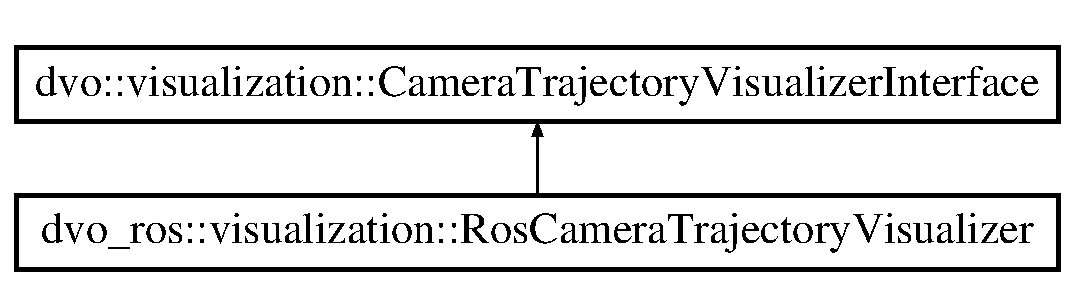
\includegraphics[height=2.000000cm]{classdvo__ros_1_1visualization_1_1_ros_camera_trajectory_visualizer}
\end{center}
\end{figure}
\subsection*{Public Member Functions}
\begin{DoxyCompactItemize}
\item 
\mbox{\hyperlink{classdvo__ros_1_1visualization_1_1_ros_camera_trajectory_visualizer_ac1ea5f7ec4b70001b9f10ff7ebfe5196}{Ros\+Camera\+Trajectory\+Visualizer}} (ros\+::\+Node\+Handle \&nh)
\item 
virtual \mbox{\hyperlink{classdvo__ros_1_1visualization_1_1_ros_camera_trajectory_visualizer_a06555d4a1a53b4deda6f86fde360ca73}{$\sim$\+Ros\+Camera\+Trajectory\+Visualizer}} ()
\item 
virtual \mbox{\hyperlink{classdvo_1_1visualization_1_1_camera_visualizer_a473ebecc62e1d4edba21027d858789a2}{dvo\+::visualization\+::\+Camera\+Visualizer\+::\+Ptr}} \mbox{\hyperlink{classdvo__ros_1_1visualization_1_1_ros_camera_trajectory_visualizer_a9595c8a8bfceffb2da725b462569404c}{camera}} (std\+::string name)
\item 
virtual \mbox{\hyperlink{classdvo_1_1visualization_1_1_trajectory_visualizer_aac33ef5979fe64ee33409f1afa977fd3}{dvo\+::visualization\+::\+Trajectory\+Visualizer\+::\+Ptr}} \mbox{\hyperlink{classdvo__ros_1_1visualization_1_1_ros_camera_trajectory_visualizer_a3a015885211d1dfac2441ab5f0e26af5}{trajectory}} (std\+::string name)
\item 
virtual void \mbox{\hyperlink{classdvo__ros_1_1visualization_1_1_ros_camera_trajectory_visualizer_a1900ce8a2c17014fef1a4375d8fd6e92}{reset}} ()
\item 
virtual bool \mbox{\hyperlink{classdvo__ros_1_1visualization_1_1_ros_camera_trajectory_visualizer_a2e5c80d7dc8308ac038be2e4b71f4e25}{native}} (void $\ast$\&native\+\_\+visualizer)
\end{DoxyCompactItemize}


\subsection{Constructor \& Destructor Documentation}
\mbox{\Hypertarget{classdvo__ros_1_1visualization_1_1_ros_camera_trajectory_visualizer_ac1ea5f7ec4b70001b9f10ff7ebfe5196}\label{classdvo__ros_1_1visualization_1_1_ros_camera_trajectory_visualizer_ac1ea5f7ec4b70001b9f10ff7ebfe5196}} 
\index{dvo\+\_\+ros\+::visualization\+::\+Ros\+Camera\+Trajectory\+Visualizer@{dvo\+\_\+ros\+::visualization\+::\+Ros\+Camera\+Trajectory\+Visualizer}!Ros\+Camera\+Trajectory\+Visualizer@{Ros\+Camera\+Trajectory\+Visualizer}}
\index{Ros\+Camera\+Trajectory\+Visualizer@{Ros\+Camera\+Trajectory\+Visualizer}!dvo\+\_\+ros\+::visualization\+::\+Ros\+Camera\+Trajectory\+Visualizer@{dvo\+\_\+ros\+::visualization\+::\+Ros\+Camera\+Trajectory\+Visualizer}}
\subsubsection{\texorpdfstring{Ros\+Camera\+Trajectory\+Visualizer()}{RosCameraTrajectoryVisualizer()}}
{\footnotesize\ttfamily dvo\+\_\+ros\+::visualization\+::\+Ros\+Camera\+Trajectory\+Visualizer\+::\+Ros\+Camera\+Trajectory\+Visualizer (\begin{DoxyParamCaption}\item[{ros\+::\+Node\+Handle \&}]{nh }\end{DoxyParamCaption})}

\mbox{\Hypertarget{classdvo__ros_1_1visualization_1_1_ros_camera_trajectory_visualizer_a06555d4a1a53b4deda6f86fde360ca73}\label{classdvo__ros_1_1visualization_1_1_ros_camera_trajectory_visualizer_a06555d4a1a53b4deda6f86fde360ca73}} 
\index{dvo\+\_\+ros\+::visualization\+::\+Ros\+Camera\+Trajectory\+Visualizer@{dvo\+\_\+ros\+::visualization\+::\+Ros\+Camera\+Trajectory\+Visualizer}!````~Ros\+Camera\+Trajectory\+Visualizer@{$\sim$\+Ros\+Camera\+Trajectory\+Visualizer}}
\index{````~Ros\+Camera\+Trajectory\+Visualizer@{$\sim$\+Ros\+Camera\+Trajectory\+Visualizer}!dvo\+\_\+ros\+::visualization\+::\+Ros\+Camera\+Trajectory\+Visualizer@{dvo\+\_\+ros\+::visualization\+::\+Ros\+Camera\+Trajectory\+Visualizer}}
\subsubsection{\texorpdfstring{$\sim$\+Ros\+Camera\+Trajectory\+Visualizer()}{~RosCameraTrajectoryVisualizer()}}
{\footnotesize\ttfamily dvo\+\_\+ros\+::visualization\+::\+Ros\+Camera\+Trajectory\+Visualizer\+::$\sim$\+Ros\+Camera\+Trajectory\+Visualizer (\begin{DoxyParamCaption}{ }\end{DoxyParamCaption})\hspace{0.3cm}{\ttfamily [virtual]}}



\subsection{Member Function Documentation}
\mbox{\Hypertarget{classdvo__ros_1_1visualization_1_1_ros_camera_trajectory_visualizer_a9595c8a8bfceffb2da725b462569404c}\label{classdvo__ros_1_1visualization_1_1_ros_camera_trajectory_visualizer_a9595c8a8bfceffb2da725b462569404c}} 
\index{dvo\+\_\+ros\+::visualization\+::\+Ros\+Camera\+Trajectory\+Visualizer@{dvo\+\_\+ros\+::visualization\+::\+Ros\+Camera\+Trajectory\+Visualizer}!camera@{camera}}
\index{camera@{camera}!dvo\+\_\+ros\+::visualization\+::\+Ros\+Camera\+Trajectory\+Visualizer@{dvo\+\_\+ros\+::visualization\+::\+Ros\+Camera\+Trajectory\+Visualizer}}
\subsubsection{\texorpdfstring{camera()}{camera()}}
{\footnotesize\ttfamily \mbox{\hyperlink{classdvo_1_1visualization_1_1_camera_visualizer_a473ebecc62e1d4edba21027d858789a2}{dvo\+::visualization\+::\+Camera\+Visualizer\+::\+Ptr}} dvo\+\_\+ros\+::visualization\+::\+Ros\+Camera\+Trajectory\+Visualizer\+::camera (\begin{DoxyParamCaption}\item[{std\+::string}]{name }\end{DoxyParamCaption})\hspace{0.3cm}{\ttfamily [virtual]}}



Implements \mbox{\hyperlink{classdvo_1_1visualization_1_1_camera_trajectory_visualizer_interface_a4d43cd43f26bd880eb07e8ee37a7154a}{dvo\+::visualization\+::\+Camera\+Trajectory\+Visualizer\+Interface}}.

\mbox{\Hypertarget{classdvo__ros_1_1visualization_1_1_ros_camera_trajectory_visualizer_a2e5c80d7dc8308ac038be2e4b71f4e25}\label{classdvo__ros_1_1visualization_1_1_ros_camera_trajectory_visualizer_a2e5c80d7dc8308ac038be2e4b71f4e25}} 
\index{dvo\+\_\+ros\+::visualization\+::\+Ros\+Camera\+Trajectory\+Visualizer@{dvo\+\_\+ros\+::visualization\+::\+Ros\+Camera\+Trajectory\+Visualizer}!native@{native}}
\index{native@{native}!dvo\+\_\+ros\+::visualization\+::\+Ros\+Camera\+Trajectory\+Visualizer@{dvo\+\_\+ros\+::visualization\+::\+Ros\+Camera\+Trajectory\+Visualizer}}
\subsubsection{\texorpdfstring{native()}{native()}}
{\footnotesize\ttfamily bool dvo\+\_\+ros\+::visualization\+::\+Ros\+Camera\+Trajectory\+Visualizer\+::native (\begin{DoxyParamCaption}\item[{void $\ast$\&}]{native\+\_\+visualizer }\end{DoxyParamCaption})\hspace{0.3cm}{\ttfamily [virtual]}}



Reimplemented from \mbox{\hyperlink{classdvo_1_1visualization_1_1_camera_trajectory_visualizer_interface_aa034546bfbdfa55855c56ab21df41b8e}{dvo\+::visualization\+::\+Camera\+Trajectory\+Visualizer\+Interface}}.

\mbox{\Hypertarget{classdvo__ros_1_1visualization_1_1_ros_camera_trajectory_visualizer_a1900ce8a2c17014fef1a4375d8fd6e92}\label{classdvo__ros_1_1visualization_1_1_ros_camera_trajectory_visualizer_a1900ce8a2c17014fef1a4375d8fd6e92}} 
\index{dvo\+\_\+ros\+::visualization\+::\+Ros\+Camera\+Trajectory\+Visualizer@{dvo\+\_\+ros\+::visualization\+::\+Ros\+Camera\+Trajectory\+Visualizer}!reset@{reset}}
\index{reset@{reset}!dvo\+\_\+ros\+::visualization\+::\+Ros\+Camera\+Trajectory\+Visualizer@{dvo\+\_\+ros\+::visualization\+::\+Ros\+Camera\+Trajectory\+Visualizer}}
\subsubsection{\texorpdfstring{reset()}{reset()}}
{\footnotesize\ttfamily void dvo\+\_\+ros\+::visualization\+::\+Ros\+Camera\+Trajectory\+Visualizer\+::reset (\begin{DoxyParamCaption}{ }\end{DoxyParamCaption})\hspace{0.3cm}{\ttfamily [virtual]}}



Implements \mbox{\hyperlink{classdvo_1_1visualization_1_1_camera_trajectory_visualizer_interface_abcc7ddffc30b41eb9112c386f3e41aa7}{dvo\+::visualization\+::\+Camera\+Trajectory\+Visualizer\+Interface}}.

\mbox{\Hypertarget{classdvo__ros_1_1visualization_1_1_ros_camera_trajectory_visualizer_a3a015885211d1dfac2441ab5f0e26af5}\label{classdvo__ros_1_1visualization_1_1_ros_camera_trajectory_visualizer_a3a015885211d1dfac2441ab5f0e26af5}} 
\index{dvo\+\_\+ros\+::visualization\+::\+Ros\+Camera\+Trajectory\+Visualizer@{dvo\+\_\+ros\+::visualization\+::\+Ros\+Camera\+Trajectory\+Visualizer}!trajectory@{trajectory}}
\index{trajectory@{trajectory}!dvo\+\_\+ros\+::visualization\+::\+Ros\+Camera\+Trajectory\+Visualizer@{dvo\+\_\+ros\+::visualization\+::\+Ros\+Camera\+Trajectory\+Visualizer}}
\subsubsection{\texorpdfstring{trajectory()}{trajectory()}}
{\footnotesize\ttfamily \mbox{\hyperlink{classdvo_1_1visualization_1_1_trajectory_visualizer_aac33ef5979fe64ee33409f1afa977fd3}{dvo\+::visualization\+::\+Trajectory\+Visualizer\+::\+Ptr}} dvo\+\_\+ros\+::visualization\+::\+Ros\+Camera\+Trajectory\+Visualizer\+::trajectory (\begin{DoxyParamCaption}\item[{std\+::string}]{name }\end{DoxyParamCaption})\hspace{0.3cm}{\ttfamily [virtual]}}



Implements \mbox{\hyperlink{classdvo_1_1visualization_1_1_camera_trajectory_visualizer_interface_ac658e841335e51c50325267de10e64b3}{dvo\+::visualization\+::\+Camera\+Trajectory\+Visualizer\+Interface}}.



The documentation for this class was generated from the following files\+:\begin{DoxyCompactItemize}
\item 
dvo\+\_\+ros/include/dvo\+\_\+ros/visualization/\mbox{\hyperlink{ros__camera__trajectory__visualizer_8h}{ros\+\_\+camera\+\_\+trajectory\+\_\+visualizer.\+h}}\item 
dvo\+\_\+ros/src/visualization/\mbox{\hyperlink{ros__camera__trajectory__visualizer_8cpp}{ros\+\_\+camera\+\_\+trajectory\+\_\+visualizer.\+cpp}}\end{DoxyCompactItemize}

\hypertarget{structdvo__ros_1_1visualization_1_1internal_1_1_ros_camera_trajectory_visualizer_impl}{}\section{dvo\+\_\+ros\+:\+:visualization\+:\+:internal\+:\+:Ros\+Camera\+Trajectory\+Visualizer\+Impl Struct Reference}
\label{structdvo__ros_1_1visualization_1_1internal_1_1_ros_camera_trajectory_visualizer_impl}\index{dvo\+\_\+ros\+::visualization\+::internal\+::\+Ros\+Camera\+Trajectory\+Visualizer\+Impl@{dvo\+\_\+ros\+::visualization\+::internal\+::\+Ros\+Camera\+Trajectory\+Visualizer\+Impl}}
\subsection*{Public Types}
\begin{DoxyCompactItemize}
\item 
typedef std\+::map$<$ std\+::string, \mbox{\hyperlink{classdvo_1_1visualization_1_1_camera_visualizer_a473ebecc62e1d4edba21027d858789a2}{Camera\+Visualizer\+::\+Ptr}} $>$ \mbox{\hyperlink{structdvo__ros_1_1visualization_1_1internal_1_1_ros_camera_trajectory_visualizer_impl_a9eafaee3bd7de4182a58c268cab6d86d}{Camera\+Visualizer\+Map}}
\item 
typedef std\+::map$<$ std\+::string, \mbox{\hyperlink{classdvo_1_1visualization_1_1_trajectory_visualizer_aac33ef5979fe64ee33409f1afa977fd3}{Trajectory\+Visualizer\+::\+Ptr}} $>$ \mbox{\hyperlink{structdvo__ros_1_1visualization_1_1internal_1_1_ros_camera_trajectory_visualizer_impl_a39e2bcdbb593f2f60778e908dda9b0cd}{Trajectory\+Visualizer\+Map}}
\end{DoxyCompactItemize}
\subsection*{Public Member Functions}
\begin{DoxyCompactItemize}
\item 
\mbox{\hyperlink{structdvo__ros_1_1visualization_1_1internal_1_1_ros_camera_trajectory_visualizer_impl_aeb26a5141f9cbf9e6a4524a921212e32}{Ros\+Camera\+Trajectory\+Visualizer\+Impl}} (ros\+::\+Node\+Handle \&nh)
\item 
\mbox{\hyperlink{structdvo__ros_1_1visualization_1_1internal_1_1_ros_camera_trajectory_visualizer_impl_a7d3fbd3917e5db9817504e69efccbc9f}{$\sim$\+Ros\+Camera\+Trajectory\+Visualizer\+Impl}} ()
\item 
\mbox{\hyperlink{classdvo_1_1visualization_1_1_camera_visualizer_a473ebecc62e1d4edba21027d858789a2}{Camera\+Visualizer\+::\+Ptr}} \mbox{\hyperlink{structdvo__ros_1_1visualization_1_1internal_1_1_ros_camera_trajectory_visualizer_impl_afeba7110c0c1404ad84783463e623f11}{camera}} (std\+::string name)
\item 
\mbox{\hyperlink{classdvo_1_1visualization_1_1_trajectory_visualizer_aac33ef5979fe64ee33409f1afa977fd3}{Trajectory\+Visualizer\+::\+Ptr}} \mbox{\hyperlink{structdvo__ros_1_1visualization_1_1internal_1_1_ros_camera_trajectory_visualizer_impl_a1228b6fa3e346cc73f40e3231b8570ef}{trajectory}} (std\+::string name)
\item 
void \mbox{\hyperlink{structdvo__ros_1_1visualization_1_1internal_1_1_ros_camera_trajectory_visualizer_impl_ac5fdbb6bd75618ea9f11cbef6304806f}{reset}} ()
\item 
interactive\+\_\+markers\+::\+Interactive\+Marker\+Server $\ast$ \mbox{\hyperlink{structdvo__ros_1_1visualization_1_1internal_1_1_ros_camera_trajectory_visualizer_impl_add4ff5e56f40ef64943d3a3018e8d222}{native}} ()
\end{DoxyCompactItemize}


\subsection{Member Typedef Documentation}
\mbox{\Hypertarget{structdvo__ros_1_1visualization_1_1internal_1_1_ros_camera_trajectory_visualizer_impl_a9eafaee3bd7de4182a58c268cab6d86d}\label{structdvo__ros_1_1visualization_1_1internal_1_1_ros_camera_trajectory_visualizer_impl_a9eafaee3bd7de4182a58c268cab6d86d}} 
\index{dvo\+\_\+ros\+::visualization\+::internal\+::\+Ros\+Camera\+Trajectory\+Visualizer\+Impl@{dvo\+\_\+ros\+::visualization\+::internal\+::\+Ros\+Camera\+Trajectory\+Visualizer\+Impl}!Camera\+Visualizer\+Map@{Camera\+Visualizer\+Map}}
\index{Camera\+Visualizer\+Map@{Camera\+Visualizer\+Map}!dvo\+\_\+ros\+::visualization\+::internal\+::\+Ros\+Camera\+Trajectory\+Visualizer\+Impl@{dvo\+\_\+ros\+::visualization\+::internal\+::\+Ros\+Camera\+Trajectory\+Visualizer\+Impl}}
\subsubsection{\texorpdfstring{Camera\+Visualizer\+Map}{CameraVisualizerMap}}
{\footnotesize\ttfamily typedef std\+::map$<$std\+::string, \mbox{\hyperlink{classdvo_1_1visualization_1_1_camera_visualizer_a473ebecc62e1d4edba21027d858789a2}{Camera\+Visualizer\+::\+Ptr}}$>$ \mbox{\hyperlink{structdvo__ros_1_1visualization_1_1internal_1_1_ros_camera_trajectory_visualizer_impl_a9eafaee3bd7de4182a58c268cab6d86d}{dvo\+\_\+ros\+::visualization\+::internal\+::\+Ros\+Camera\+Trajectory\+Visualizer\+Impl\+::\+Camera\+Visualizer\+Map}}}

\mbox{\Hypertarget{structdvo__ros_1_1visualization_1_1internal_1_1_ros_camera_trajectory_visualizer_impl_a39e2bcdbb593f2f60778e908dda9b0cd}\label{structdvo__ros_1_1visualization_1_1internal_1_1_ros_camera_trajectory_visualizer_impl_a39e2bcdbb593f2f60778e908dda9b0cd}} 
\index{dvo\+\_\+ros\+::visualization\+::internal\+::\+Ros\+Camera\+Trajectory\+Visualizer\+Impl@{dvo\+\_\+ros\+::visualization\+::internal\+::\+Ros\+Camera\+Trajectory\+Visualizer\+Impl}!Trajectory\+Visualizer\+Map@{Trajectory\+Visualizer\+Map}}
\index{Trajectory\+Visualizer\+Map@{Trajectory\+Visualizer\+Map}!dvo\+\_\+ros\+::visualization\+::internal\+::\+Ros\+Camera\+Trajectory\+Visualizer\+Impl@{dvo\+\_\+ros\+::visualization\+::internal\+::\+Ros\+Camera\+Trajectory\+Visualizer\+Impl}}
\subsubsection{\texorpdfstring{Trajectory\+Visualizer\+Map}{TrajectoryVisualizerMap}}
{\footnotesize\ttfamily typedef std\+::map$<$std\+::string, \mbox{\hyperlink{classdvo_1_1visualization_1_1_trajectory_visualizer_aac33ef5979fe64ee33409f1afa977fd3}{Trajectory\+Visualizer\+::\+Ptr}}$>$ \mbox{\hyperlink{structdvo__ros_1_1visualization_1_1internal_1_1_ros_camera_trajectory_visualizer_impl_a39e2bcdbb593f2f60778e908dda9b0cd}{dvo\+\_\+ros\+::visualization\+::internal\+::\+Ros\+Camera\+Trajectory\+Visualizer\+Impl\+::\+Trajectory\+Visualizer\+Map}}}



\subsection{Constructor \& Destructor Documentation}
\mbox{\Hypertarget{structdvo__ros_1_1visualization_1_1internal_1_1_ros_camera_trajectory_visualizer_impl_aeb26a5141f9cbf9e6a4524a921212e32}\label{structdvo__ros_1_1visualization_1_1internal_1_1_ros_camera_trajectory_visualizer_impl_aeb26a5141f9cbf9e6a4524a921212e32}} 
\index{dvo\+\_\+ros\+::visualization\+::internal\+::\+Ros\+Camera\+Trajectory\+Visualizer\+Impl@{dvo\+\_\+ros\+::visualization\+::internal\+::\+Ros\+Camera\+Trajectory\+Visualizer\+Impl}!Ros\+Camera\+Trajectory\+Visualizer\+Impl@{Ros\+Camera\+Trajectory\+Visualizer\+Impl}}
\index{Ros\+Camera\+Trajectory\+Visualizer\+Impl@{Ros\+Camera\+Trajectory\+Visualizer\+Impl}!dvo\+\_\+ros\+::visualization\+::internal\+::\+Ros\+Camera\+Trajectory\+Visualizer\+Impl@{dvo\+\_\+ros\+::visualization\+::internal\+::\+Ros\+Camera\+Trajectory\+Visualizer\+Impl}}
\subsubsection{\texorpdfstring{Ros\+Camera\+Trajectory\+Visualizer\+Impl()}{RosCameraTrajectoryVisualizerImpl()}}
{\footnotesize\ttfamily dvo\+\_\+ros\+::visualization\+::internal\+::\+Ros\+Camera\+Trajectory\+Visualizer\+Impl\+::\+Ros\+Camera\+Trajectory\+Visualizer\+Impl (\begin{DoxyParamCaption}\item[{ros\+::\+Node\+Handle \&}]{nh }\end{DoxyParamCaption})\hspace{0.3cm}{\ttfamily [inline]}}

\mbox{\Hypertarget{structdvo__ros_1_1visualization_1_1internal_1_1_ros_camera_trajectory_visualizer_impl_a7d3fbd3917e5db9817504e69efccbc9f}\label{structdvo__ros_1_1visualization_1_1internal_1_1_ros_camera_trajectory_visualizer_impl_a7d3fbd3917e5db9817504e69efccbc9f}} 
\index{dvo\+\_\+ros\+::visualization\+::internal\+::\+Ros\+Camera\+Trajectory\+Visualizer\+Impl@{dvo\+\_\+ros\+::visualization\+::internal\+::\+Ros\+Camera\+Trajectory\+Visualizer\+Impl}!````~Ros\+Camera\+Trajectory\+Visualizer\+Impl@{$\sim$\+Ros\+Camera\+Trajectory\+Visualizer\+Impl}}
\index{````~Ros\+Camera\+Trajectory\+Visualizer\+Impl@{$\sim$\+Ros\+Camera\+Trajectory\+Visualizer\+Impl}!dvo\+\_\+ros\+::visualization\+::internal\+::\+Ros\+Camera\+Trajectory\+Visualizer\+Impl@{dvo\+\_\+ros\+::visualization\+::internal\+::\+Ros\+Camera\+Trajectory\+Visualizer\+Impl}}
\subsubsection{\texorpdfstring{$\sim$\+Ros\+Camera\+Trajectory\+Visualizer\+Impl()}{~RosCameraTrajectoryVisualizerImpl()}}
{\footnotesize\ttfamily dvo\+\_\+ros\+::visualization\+::internal\+::\+Ros\+Camera\+Trajectory\+Visualizer\+Impl\+::$\sim$\+Ros\+Camera\+Trajectory\+Visualizer\+Impl (\begin{DoxyParamCaption}{ }\end{DoxyParamCaption})\hspace{0.3cm}{\ttfamily [inline]}}



\subsection{Member Function Documentation}
\mbox{\Hypertarget{structdvo__ros_1_1visualization_1_1internal_1_1_ros_camera_trajectory_visualizer_impl_afeba7110c0c1404ad84783463e623f11}\label{structdvo__ros_1_1visualization_1_1internal_1_1_ros_camera_trajectory_visualizer_impl_afeba7110c0c1404ad84783463e623f11}} 
\index{dvo\+\_\+ros\+::visualization\+::internal\+::\+Ros\+Camera\+Trajectory\+Visualizer\+Impl@{dvo\+\_\+ros\+::visualization\+::internal\+::\+Ros\+Camera\+Trajectory\+Visualizer\+Impl}!camera@{camera}}
\index{camera@{camera}!dvo\+\_\+ros\+::visualization\+::internal\+::\+Ros\+Camera\+Trajectory\+Visualizer\+Impl@{dvo\+\_\+ros\+::visualization\+::internal\+::\+Ros\+Camera\+Trajectory\+Visualizer\+Impl}}
\subsubsection{\texorpdfstring{camera()}{camera()}}
{\footnotesize\ttfamily \mbox{\hyperlink{classdvo_1_1visualization_1_1_camera_visualizer_a473ebecc62e1d4edba21027d858789a2}{Camera\+Visualizer\+::\+Ptr}} dvo\+\_\+ros\+::visualization\+::internal\+::\+Ros\+Camera\+Trajectory\+Visualizer\+Impl\+::camera (\begin{DoxyParamCaption}\item[{std\+::string}]{name }\end{DoxyParamCaption})\hspace{0.3cm}{\ttfamily [inline]}}

\mbox{\Hypertarget{structdvo__ros_1_1visualization_1_1internal_1_1_ros_camera_trajectory_visualizer_impl_add4ff5e56f40ef64943d3a3018e8d222}\label{structdvo__ros_1_1visualization_1_1internal_1_1_ros_camera_trajectory_visualizer_impl_add4ff5e56f40ef64943d3a3018e8d222}} 
\index{dvo\+\_\+ros\+::visualization\+::internal\+::\+Ros\+Camera\+Trajectory\+Visualizer\+Impl@{dvo\+\_\+ros\+::visualization\+::internal\+::\+Ros\+Camera\+Trajectory\+Visualizer\+Impl}!native@{native}}
\index{native@{native}!dvo\+\_\+ros\+::visualization\+::internal\+::\+Ros\+Camera\+Trajectory\+Visualizer\+Impl@{dvo\+\_\+ros\+::visualization\+::internal\+::\+Ros\+Camera\+Trajectory\+Visualizer\+Impl}}
\subsubsection{\texorpdfstring{native()}{native()}}
{\footnotesize\ttfamily interactive\+\_\+markers\+::\+Interactive\+Marker\+Server$\ast$ dvo\+\_\+ros\+::visualization\+::internal\+::\+Ros\+Camera\+Trajectory\+Visualizer\+Impl\+::native (\begin{DoxyParamCaption}{ }\end{DoxyParamCaption})\hspace{0.3cm}{\ttfamily [inline]}}

\mbox{\Hypertarget{structdvo__ros_1_1visualization_1_1internal_1_1_ros_camera_trajectory_visualizer_impl_ac5fdbb6bd75618ea9f11cbef6304806f}\label{structdvo__ros_1_1visualization_1_1internal_1_1_ros_camera_trajectory_visualizer_impl_ac5fdbb6bd75618ea9f11cbef6304806f}} 
\index{dvo\+\_\+ros\+::visualization\+::internal\+::\+Ros\+Camera\+Trajectory\+Visualizer\+Impl@{dvo\+\_\+ros\+::visualization\+::internal\+::\+Ros\+Camera\+Trajectory\+Visualizer\+Impl}!reset@{reset}}
\index{reset@{reset}!dvo\+\_\+ros\+::visualization\+::internal\+::\+Ros\+Camera\+Trajectory\+Visualizer\+Impl@{dvo\+\_\+ros\+::visualization\+::internal\+::\+Ros\+Camera\+Trajectory\+Visualizer\+Impl}}
\subsubsection{\texorpdfstring{reset()}{reset()}}
{\footnotesize\ttfamily void dvo\+\_\+ros\+::visualization\+::internal\+::\+Ros\+Camera\+Trajectory\+Visualizer\+Impl\+::reset (\begin{DoxyParamCaption}{ }\end{DoxyParamCaption})\hspace{0.3cm}{\ttfamily [inline]}}

\mbox{\Hypertarget{structdvo__ros_1_1visualization_1_1internal_1_1_ros_camera_trajectory_visualizer_impl_a1228b6fa3e346cc73f40e3231b8570ef}\label{structdvo__ros_1_1visualization_1_1internal_1_1_ros_camera_trajectory_visualizer_impl_a1228b6fa3e346cc73f40e3231b8570ef}} 
\index{dvo\+\_\+ros\+::visualization\+::internal\+::\+Ros\+Camera\+Trajectory\+Visualizer\+Impl@{dvo\+\_\+ros\+::visualization\+::internal\+::\+Ros\+Camera\+Trajectory\+Visualizer\+Impl}!trajectory@{trajectory}}
\index{trajectory@{trajectory}!dvo\+\_\+ros\+::visualization\+::internal\+::\+Ros\+Camera\+Trajectory\+Visualizer\+Impl@{dvo\+\_\+ros\+::visualization\+::internal\+::\+Ros\+Camera\+Trajectory\+Visualizer\+Impl}}
\subsubsection{\texorpdfstring{trajectory()}{trajectory()}}
{\footnotesize\ttfamily \mbox{\hyperlink{classdvo_1_1visualization_1_1_trajectory_visualizer_aac33ef5979fe64ee33409f1afa977fd3}{Trajectory\+Visualizer\+::\+Ptr}} dvo\+\_\+ros\+::visualization\+::internal\+::\+Ros\+Camera\+Trajectory\+Visualizer\+Impl\+::trajectory (\begin{DoxyParamCaption}\item[{std\+::string}]{name }\end{DoxyParamCaption})\hspace{0.3cm}{\ttfamily [inline]}}



The documentation for this struct was generated from the following file\+:\begin{DoxyCompactItemize}
\item 
dvo\+\_\+ros/src/visualization/\mbox{\hyperlink{ros__camera__trajectory__visualizer_8cpp}{ros\+\_\+camera\+\_\+trajectory\+\_\+visualizer.\+cpp}}\end{DoxyCompactItemize}

\hypertarget{classdvo__ros_1_1visualization_1_1internal_1_1_ros_camera_visualizer}{}\section{dvo\+\_\+ros\+:\+:visualization\+:\+:internal\+:\+:Ros\+Camera\+Visualizer Class Reference}
\label{classdvo__ros_1_1visualization_1_1internal_1_1_ros_camera_visualizer}\index{dvo\+\_\+ros\+::visualization\+::internal\+::\+Ros\+Camera\+Visualizer@{dvo\+\_\+ros\+::visualization\+::internal\+::\+Ros\+Camera\+Visualizer}}
Inheritance diagram for dvo\+\_\+ros\+:\+:visualization\+:\+:internal\+:\+:Ros\+Camera\+Visualizer\+:\begin{figure}[H]
\begin{center}
\leavevmode
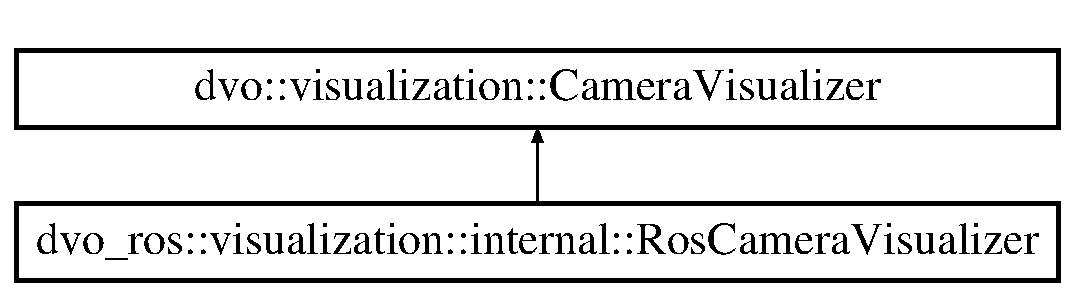
\includegraphics[height=2.000000cm]{classdvo__ros_1_1visualization_1_1internal_1_1_ros_camera_visualizer}
\end{center}
\end{figure}
\subsection*{Public Member Functions}
\begin{DoxyCompactItemize}
\item 
\mbox{\hyperlink{classdvo__ros_1_1visualization_1_1internal_1_1_ros_camera_visualizer_a48e16edb7cb922fd824f4733b775d0b6}{Ros\+Camera\+Visualizer}} (std\+::string name, interactive\+\_\+markers\+::\+Interactive\+Marker\+Server \&marker\+\_\+server, \mbox{\hyperlink{classdvo_1_1visualization_1_1_point_cloud_aggregator}{dvo\+::visualization\+::\+Point\+Cloud\+Aggregator}} \&point\+\_\+cloud\+\_\+aggregator)
\item 
virtual \mbox{\hyperlink{classdvo__ros_1_1visualization_1_1internal_1_1_ros_camera_visualizer_aec973f21c7f3bc77ab4253b86f370dbf}{$\sim$\+Ros\+Camera\+Visualizer}} ()
\item 
virtual void \mbox{\hyperlink{classdvo__ros_1_1visualization_1_1internal_1_1_ros_camera_visualizer_afb9b360caa2de42ad4b9fd55c85b98df}{show}} (\mbox{\hyperlink{classdvo_1_1visualization_1_1_camera_visualizer_a0526f50be9f298c4f7d1f91018d50af7}{Option}} option=\mbox{\hyperlink{classdvo_1_1visualization_1_1_camera_visualizer_a0526f50be9f298c4f7d1f91018d50af7a0ff8fc7d7283f27066e93ca0d4ef3f19}{Show\+Camera\+And\+Cloud}})
\item 
virtual void \mbox{\hyperlink{classdvo__ros_1_1visualization_1_1internal_1_1_ros_camera_visualizer_a4812a8e3c5573a68fb74cabbf2f70422}{hide}} ()
\item 
virtual \mbox{\hyperlink{classdvo_1_1visualization_1_1_camera_visualizer}{Camera\+Visualizer}} \& \mbox{\hyperlink{classdvo__ros_1_1visualization_1_1internal_1_1_ros_camera_visualizer_aa347218752bde73e09874771fe3b4410}{update}} (const \mbox{\hyperlink{structdvo_1_1core_1_1_rgbd_image}{dvo\+::core\+::\+Rgbd\+Image}} \&img, const \mbox{\hyperlink{structdvo_1_1core_1_1_intrinsic_matrix}{dvo\+::core\+::\+Intrinsic\+Matrix}} \&intrinsics, const Eigen\+::\+Affine3d \&pose)
\end{DoxyCompactItemize}
\subsection*{Additional Inherited Members}


\subsection{Constructor \& Destructor Documentation}
\mbox{\Hypertarget{classdvo__ros_1_1visualization_1_1internal_1_1_ros_camera_visualizer_a48e16edb7cb922fd824f4733b775d0b6}\label{classdvo__ros_1_1visualization_1_1internal_1_1_ros_camera_visualizer_a48e16edb7cb922fd824f4733b775d0b6}} 
\index{dvo\+\_\+ros\+::visualization\+::internal\+::\+Ros\+Camera\+Visualizer@{dvo\+\_\+ros\+::visualization\+::internal\+::\+Ros\+Camera\+Visualizer}!Ros\+Camera\+Visualizer@{Ros\+Camera\+Visualizer}}
\index{Ros\+Camera\+Visualizer@{Ros\+Camera\+Visualizer}!dvo\+\_\+ros\+::visualization\+::internal\+::\+Ros\+Camera\+Visualizer@{dvo\+\_\+ros\+::visualization\+::internal\+::\+Ros\+Camera\+Visualizer}}
\subsubsection{\texorpdfstring{Ros\+Camera\+Visualizer()}{RosCameraVisualizer()}}
{\footnotesize\ttfamily dvo\+\_\+ros\+::visualization\+::internal\+::\+Ros\+Camera\+Visualizer\+::\+Ros\+Camera\+Visualizer (\begin{DoxyParamCaption}\item[{std\+::string}]{name,  }\item[{interactive\+\_\+markers\+::\+Interactive\+Marker\+Server \&}]{marker\+\_\+server,  }\item[{\mbox{\hyperlink{classdvo_1_1visualization_1_1_point_cloud_aggregator}{dvo\+::visualization\+::\+Point\+Cloud\+Aggregator}} \&}]{point\+\_\+cloud\+\_\+aggregator }\end{DoxyParamCaption})\hspace{0.3cm}{\ttfamily [inline]}}

\mbox{\Hypertarget{classdvo__ros_1_1visualization_1_1internal_1_1_ros_camera_visualizer_aec973f21c7f3bc77ab4253b86f370dbf}\label{classdvo__ros_1_1visualization_1_1internal_1_1_ros_camera_visualizer_aec973f21c7f3bc77ab4253b86f370dbf}} 
\index{dvo\+\_\+ros\+::visualization\+::internal\+::\+Ros\+Camera\+Visualizer@{dvo\+\_\+ros\+::visualization\+::internal\+::\+Ros\+Camera\+Visualizer}!````~Ros\+Camera\+Visualizer@{$\sim$\+Ros\+Camera\+Visualizer}}
\index{````~Ros\+Camera\+Visualizer@{$\sim$\+Ros\+Camera\+Visualizer}!dvo\+\_\+ros\+::visualization\+::internal\+::\+Ros\+Camera\+Visualizer@{dvo\+\_\+ros\+::visualization\+::internal\+::\+Ros\+Camera\+Visualizer}}
\subsubsection{\texorpdfstring{$\sim$\+Ros\+Camera\+Visualizer()}{~RosCameraVisualizer()}}
{\footnotesize\ttfamily virtual dvo\+\_\+ros\+::visualization\+::internal\+::\+Ros\+Camera\+Visualizer\+::$\sim$\+Ros\+Camera\+Visualizer (\begin{DoxyParamCaption}{ }\end{DoxyParamCaption})\hspace{0.3cm}{\ttfamily [inline]}, {\ttfamily [virtual]}}



\subsection{Member Function Documentation}
\mbox{\Hypertarget{classdvo__ros_1_1visualization_1_1internal_1_1_ros_camera_visualizer_a4812a8e3c5573a68fb74cabbf2f70422}\label{classdvo__ros_1_1visualization_1_1internal_1_1_ros_camera_visualizer_a4812a8e3c5573a68fb74cabbf2f70422}} 
\index{dvo\+\_\+ros\+::visualization\+::internal\+::\+Ros\+Camera\+Visualizer@{dvo\+\_\+ros\+::visualization\+::internal\+::\+Ros\+Camera\+Visualizer}!hide@{hide}}
\index{hide@{hide}!dvo\+\_\+ros\+::visualization\+::internal\+::\+Ros\+Camera\+Visualizer@{dvo\+\_\+ros\+::visualization\+::internal\+::\+Ros\+Camera\+Visualizer}}
\subsubsection{\texorpdfstring{hide()}{hide()}}
{\footnotesize\ttfamily virtual void dvo\+\_\+ros\+::visualization\+::internal\+::\+Ros\+Camera\+Visualizer\+::hide (\begin{DoxyParamCaption}{ }\end{DoxyParamCaption})\hspace{0.3cm}{\ttfamily [inline]}, {\ttfamily [virtual]}}



Implements \mbox{\hyperlink{classdvo_1_1visualization_1_1_camera_visualizer_a45dbf0d449a7b7529f7da477c676ca85}{dvo\+::visualization\+::\+Camera\+Visualizer}}.

\mbox{\Hypertarget{classdvo__ros_1_1visualization_1_1internal_1_1_ros_camera_visualizer_afb9b360caa2de42ad4b9fd55c85b98df}\label{classdvo__ros_1_1visualization_1_1internal_1_1_ros_camera_visualizer_afb9b360caa2de42ad4b9fd55c85b98df}} 
\index{dvo\+\_\+ros\+::visualization\+::internal\+::\+Ros\+Camera\+Visualizer@{dvo\+\_\+ros\+::visualization\+::internal\+::\+Ros\+Camera\+Visualizer}!show@{show}}
\index{show@{show}!dvo\+\_\+ros\+::visualization\+::internal\+::\+Ros\+Camera\+Visualizer@{dvo\+\_\+ros\+::visualization\+::internal\+::\+Ros\+Camera\+Visualizer}}
\subsubsection{\texorpdfstring{show()}{show()}}
{\footnotesize\ttfamily virtual void dvo\+\_\+ros\+::visualization\+::internal\+::\+Ros\+Camera\+Visualizer\+::show (\begin{DoxyParamCaption}\item[{\mbox{\hyperlink{classdvo_1_1visualization_1_1_camera_visualizer_a0526f50be9f298c4f7d1f91018d50af7}{Option}}}]{option = {\ttfamily \mbox{\hyperlink{classdvo_1_1visualization_1_1_camera_visualizer_a0526f50be9f298c4f7d1f91018d50af7a0ff8fc7d7283f27066e93ca0d4ef3f19}{Show\+Camera\+And\+Cloud}}} }\end{DoxyParamCaption})\hspace{0.3cm}{\ttfamily [inline]}, {\ttfamily [virtual]}}

\mbox{\Hypertarget{classdvo__ros_1_1visualization_1_1internal_1_1_ros_camera_visualizer_aa347218752bde73e09874771fe3b4410}\label{classdvo__ros_1_1visualization_1_1internal_1_1_ros_camera_visualizer_aa347218752bde73e09874771fe3b4410}} 
\index{dvo\+\_\+ros\+::visualization\+::internal\+::\+Ros\+Camera\+Visualizer@{dvo\+\_\+ros\+::visualization\+::internal\+::\+Ros\+Camera\+Visualizer}!update@{update}}
\index{update@{update}!dvo\+\_\+ros\+::visualization\+::internal\+::\+Ros\+Camera\+Visualizer@{dvo\+\_\+ros\+::visualization\+::internal\+::\+Ros\+Camera\+Visualizer}}
\subsubsection{\texorpdfstring{update()}{update()}}
{\footnotesize\ttfamily virtual \mbox{\hyperlink{classdvo_1_1visualization_1_1_camera_visualizer}{Camera\+Visualizer}}\& dvo\+\_\+ros\+::visualization\+::internal\+::\+Ros\+Camera\+Visualizer\+::update (\begin{DoxyParamCaption}\item[{const \mbox{\hyperlink{structdvo_1_1core_1_1_rgbd_image}{dvo\+::core\+::\+Rgbd\+Image}} \&}]{img,  }\item[{const \mbox{\hyperlink{structdvo_1_1core_1_1_intrinsic_matrix}{dvo\+::core\+::\+Intrinsic\+Matrix}} \&}]{intrinsics,  }\item[{const Eigen\+::\+Affine3d \&}]{pose }\end{DoxyParamCaption})\hspace{0.3cm}{\ttfamily [inline]}, {\ttfamily [virtual]}}



Implements \mbox{\hyperlink{classdvo_1_1visualization_1_1_camera_visualizer_afd83119e63048b0229820045d54c95ec}{dvo\+::visualization\+::\+Camera\+Visualizer}}.



The documentation for this class was generated from the following file\+:\begin{DoxyCompactItemize}
\item 
dvo\+\_\+ros/src/visualization/\mbox{\hyperlink{ros__camera__trajectory__visualizer_8cpp}{ros\+\_\+camera\+\_\+trajectory\+\_\+visualizer.\+cpp}}\end{DoxyCompactItemize}

\hypertarget{classdvo__ros_1_1visualization_1_1internal_1_1_ros_trajectory_visualizer}{}\section{dvo\+\_\+ros\+:\+:visualization\+:\+:internal\+:\+:Ros\+Trajectory\+Visualizer Class Reference}
\label{classdvo__ros_1_1visualization_1_1internal_1_1_ros_trajectory_visualizer}\index{dvo\+\_\+ros\+::visualization\+::internal\+::\+Ros\+Trajectory\+Visualizer@{dvo\+\_\+ros\+::visualization\+::internal\+::\+Ros\+Trajectory\+Visualizer}}
Inheritance diagram for dvo\+\_\+ros\+:\+:visualization\+:\+:internal\+:\+:Ros\+Trajectory\+Visualizer\+:\begin{figure}[H]
\begin{center}
\leavevmode
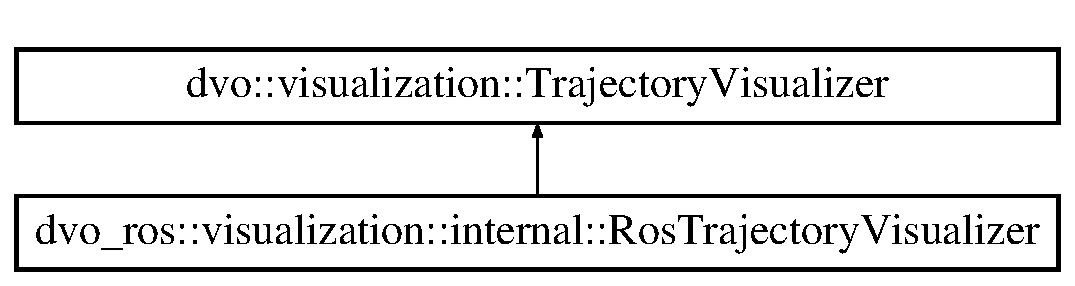
\includegraphics[height=2.000000cm]{classdvo__ros_1_1visualization_1_1internal_1_1_ros_trajectory_visualizer}
\end{center}
\end{figure}
\subsection*{Public Member Functions}
\begin{DoxyCompactItemize}
\item 
\mbox{\hyperlink{classdvo__ros_1_1visualization_1_1internal_1_1_ros_trajectory_visualizer_a374a8b54ec453c02ea55aab2c47e02c6}{Ros\+Trajectory\+Visualizer}} (std\+::string \&name, interactive\+\_\+markers\+::\+Interactive\+Marker\+Server \&marker\+\_\+server)
\item 
virtual \mbox{\hyperlink{classdvo__ros_1_1visualization_1_1internal_1_1_ros_trajectory_visualizer_a1dc0830231540aeb564421012b59ae04}{$\sim$\+Ros\+Trajectory\+Visualizer}} ()
\item 
virtual \mbox{\hyperlink{classdvo_1_1visualization_1_1_trajectory_visualizer}{Trajectory\+Visualizer}} \& \mbox{\hyperlink{classdvo__ros_1_1visualization_1_1internal_1_1_ros_trajectory_visualizer_acd66991b88e68e9843028cb5cb65c29a}{add}} (const Eigen\+::\+Affine3d \&pose)
\end{DoxyCompactItemize}
\subsection*{Additional Inherited Members}


\subsection{Constructor \& Destructor Documentation}
\mbox{\Hypertarget{classdvo__ros_1_1visualization_1_1internal_1_1_ros_trajectory_visualizer_a374a8b54ec453c02ea55aab2c47e02c6}\label{classdvo__ros_1_1visualization_1_1internal_1_1_ros_trajectory_visualizer_a374a8b54ec453c02ea55aab2c47e02c6}} 
\index{dvo\+\_\+ros\+::visualization\+::internal\+::\+Ros\+Trajectory\+Visualizer@{dvo\+\_\+ros\+::visualization\+::internal\+::\+Ros\+Trajectory\+Visualizer}!Ros\+Trajectory\+Visualizer@{Ros\+Trajectory\+Visualizer}}
\index{Ros\+Trajectory\+Visualizer@{Ros\+Trajectory\+Visualizer}!dvo\+\_\+ros\+::visualization\+::internal\+::\+Ros\+Trajectory\+Visualizer@{dvo\+\_\+ros\+::visualization\+::internal\+::\+Ros\+Trajectory\+Visualizer}}
\subsubsection{\texorpdfstring{Ros\+Trajectory\+Visualizer()}{RosTrajectoryVisualizer()}}
{\footnotesize\ttfamily dvo\+\_\+ros\+::visualization\+::internal\+::\+Ros\+Trajectory\+Visualizer\+::\+Ros\+Trajectory\+Visualizer (\begin{DoxyParamCaption}\item[{std\+::string \&}]{name,  }\item[{interactive\+\_\+markers\+::\+Interactive\+Marker\+Server \&}]{marker\+\_\+server }\end{DoxyParamCaption})\hspace{0.3cm}{\ttfamily [inline]}}

\mbox{\Hypertarget{classdvo__ros_1_1visualization_1_1internal_1_1_ros_trajectory_visualizer_a1dc0830231540aeb564421012b59ae04}\label{classdvo__ros_1_1visualization_1_1internal_1_1_ros_trajectory_visualizer_a1dc0830231540aeb564421012b59ae04}} 
\index{dvo\+\_\+ros\+::visualization\+::internal\+::\+Ros\+Trajectory\+Visualizer@{dvo\+\_\+ros\+::visualization\+::internal\+::\+Ros\+Trajectory\+Visualizer}!````~Ros\+Trajectory\+Visualizer@{$\sim$\+Ros\+Trajectory\+Visualizer}}
\index{````~Ros\+Trajectory\+Visualizer@{$\sim$\+Ros\+Trajectory\+Visualizer}!dvo\+\_\+ros\+::visualization\+::internal\+::\+Ros\+Trajectory\+Visualizer@{dvo\+\_\+ros\+::visualization\+::internal\+::\+Ros\+Trajectory\+Visualizer}}
\subsubsection{\texorpdfstring{$\sim$\+Ros\+Trajectory\+Visualizer()}{~RosTrajectoryVisualizer()}}
{\footnotesize\ttfamily virtual dvo\+\_\+ros\+::visualization\+::internal\+::\+Ros\+Trajectory\+Visualizer\+::$\sim$\+Ros\+Trajectory\+Visualizer (\begin{DoxyParamCaption}{ }\end{DoxyParamCaption})\hspace{0.3cm}{\ttfamily [inline]}, {\ttfamily [virtual]}}



\subsection{Member Function Documentation}
\mbox{\Hypertarget{classdvo__ros_1_1visualization_1_1internal_1_1_ros_trajectory_visualizer_acd66991b88e68e9843028cb5cb65c29a}\label{classdvo__ros_1_1visualization_1_1internal_1_1_ros_trajectory_visualizer_acd66991b88e68e9843028cb5cb65c29a}} 
\index{dvo\+\_\+ros\+::visualization\+::internal\+::\+Ros\+Trajectory\+Visualizer@{dvo\+\_\+ros\+::visualization\+::internal\+::\+Ros\+Trajectory\+Visualizer}!add@{add}}
\index{add@{add}!dvo\+\_\+ros\+::visualization\+::internal\+::\+Ros\+Trajectory\+Visualizer@{dvo\+\_\+ros\+::visualization\+::internal\+::\+Ros\+Trajectory\+Visualizer}}
\subsubsection{\texorpdfstring{add()}{add()}}
{\footnotesize\ttfamily virtual \mbox{\hyperlink{classdvo_1_1visualization_1_1_trajectory_visualizer}{Trajectory\+Visualizer}}\& dvo\+\_\+ros\+::visualization\+::internal\+::\+Ros\+Trajectory\+Visualizer\+::add (\begin{DoxyParamCaption}\item[{const Eigen\+::\+Affine3d \&}]{pose }\end{DoxyParamCaption})\hspace{0.3cm}{\ttfamily [inline]}, {\ttfamily [virtual]}}



Implements \mbox{\hyperlink{classdvo_1_1visualization_1_1_trajectory_visualizer_ac41106ae7e28c019b03f0aa210c6f0c1}{dvo\+::visualization\+::\+Trajectory\+Visualizer}}.



The documentation for this class was generated from the following file\+:\begin{DoxyCompactItemize}
\item 
dvo\+\_\+ros/src/visualization/\mbox{\hyperlink{ros__camera__trajectory__visualizer_8cpp}{ros\+\_\+camera\+\_\+trajectory\+\_\+visualizer.\+cpp}}\end{DoxyCompactItemize}

\hypertarget{classdvo_1_1core_1_1_scale_estimator}{}\section{dvo\+:\+:core\+:\+:Scale\+Estimator Class Reference}
\label{classdvo_1_1core_1_1_scale_estimator}\index{dvo\+::core\+::\+Scale\+Estimator@{dvo\+::core\+::\+Scale\+Estimator}}


{\ttfamily \#include $<$weight\+\_\+calculation.\+h$>$}

Inheritance diagram for dvo\+:\+:core\+:\+:Scale\+Estimator\+:\begin{figure}[H]
\begin{center}
\leavevmode
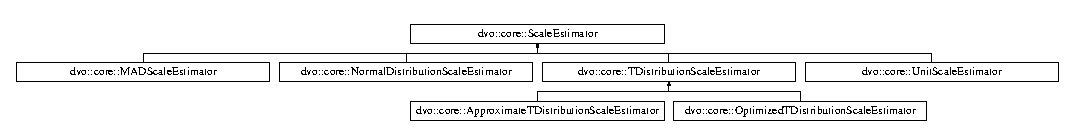
\includegraphics[height=1.390728cm]{classdvo_1_1core_1_1_scale_estimator}
\end{center}
\end{figure}
\subsection*{Public Member Functions}
\begin{DoxyCompactItemize}
\item 
virtual \mbox{\hyperlink{classdvo_1_1core_1_1_scale_estimator_a3987049356b11a891d2cad16ebbbc934}{$\sim$\+Scale\+Estimator}} ()
\item 
virtual float \mbox{\hyperlink{classdvo_1_1core_1_1_scale_estimator_a6968ac2cd37c2ce1c966f0c9e17d1a3c}{compute}} (const cv\+::\+Mat \&errors) const =0
\item 
virtual void \mbox{\hyperlink{classdvo_1_1core_1_1_scale_estimator_a58b5d7926b08e85e7393436156f3ef43}{configure}} (const float \&param)
\end{DoxyCompactItemize}


\subsection{Constructor \& Destructor Documentation}
\mbox{\Hypertarget{classdvo_1_1core_1_1_scale_estimator_a3987049356b11a891d2cad16ebbbc934}\label{classdvo_1_1core_1_1_scale_estimator_a3987049356b11a891d2cad16ebbbc934}} 
\index{dvo\+::core\+::\+Scale\+Estimator@{dvo\+::core\+::\+Scale\+Estimator}!````~Scale\+Estimator@{$\sim$\+Scale\+Estimator}}
\index{````~Scale\+Estimator@{$\sim$\+Scale\+Estimator}!dvo\+::core\+::\+Scale\+Estimator@{dvo\+::core\+::\+Scale\+Estimator}}
\subsubsection{\texorpdfstring{$\sim$\+Scale\+Estimator()}{~ScaleEstimator()}}
{\footnotesize\ttfamily virtual dvo\+::core\+::\+Scale\+Estimator\+::$\sim$\+Scale\+Estimator (\begin{DoxyParamCaption}{ }\end{DoxyParamCaption})\hspace{0.3cm}{\ttfamily [inline]}, {\ttfamily [virtual]}}



\subsection{Member Function Documentation}
\mbox{\Hypertarget{classdvo_1_1core_1_1_scale_estimator_a6968ac2cd37c2ce1c966f0c9e17d1a3c}\label{classdvo_1_1core_1_1_scale_estimator_a6968ac2cd37c2ce1c966f0c9e17d1a3c}} 
\index{dvo\+::core\+::\+Scale\+Estimator@{dvo\+::core\+::\+Scale\+Estimator}!compute@{compute}}
\index{compute@{compute}!dvo\+::core\+::\+Scale\+Estimator@{dvo\+::core\+::\+Scale\+Estimator}}
\subsubsection{\texorpdfstring{compute()}{compute()}}
{\footnotesize\ttfamily virtual float dvo\+::core\+::\+Scale\+Estimator\+::compute (\begin{DoxyParamCaption}\item[{const cv\+::\+Mat \&}]{errors }\end{DoxyParamCaption}) const\hspace{0.3cm}{\ttfamily [pure virtual]}}



Implemented in \mbox{\hyperlink{classdvo_1_1core_1_1_normal_distribution_scale_estimator_a0aa8db7144ffcd1d06704dbf89997446}{dvo\+::core\+::\+Normal\+Distribution\+Scale\+Estimator}}, \mbox{\hyperlink{classdvo_1_1core_1_1_m_a_d_scale_estimator_a421acf5af118ef5b9c394cfd5fadea1d}{dvo\+::core\+::\+M\+A\+D\+Scale\+Estimator}}, \mbox{\hyperlink{classdvo_1_1core_1_1_approximate_t_distribution_scale_estimator_aee2b37700df1eb0125b8e0d352f7ceab}{dvo\+::core\+::\+Approximate\+T\+Distribution\+Scale\+Estimator}}, \mbox{\hyperlink{classdvo_1_1core_1_1_optimized_t_distribution_scale_estimator_ace9304a785bd16a6ef5cf4a52f3c6299}{dvo\+::core\+::\+Optimized\+T\+Distribution\+Scale\+Estimator}}, \mbox{\hyperlink{classdvo_1_1core_1_1_t_distribution_scale_estimator_a0ed88ffeb9b71110e3ae69b681526bc4}{dvo\+::core\+::\+T\+Distribution\+Scale\+Estimator}}, and \mbox{\hyperlink{classdvo_1_1core_1_1_unit_scale_estimator_a7578f9008f25d96250c20ff3080673ed}{dvo\+::core\+::\+Unit\+Scale\+Estimator}}.

\mbox{\Hypertarget{classdvo_1_1core_1_1_scale_estimator_a58b5d7926b08e85e7393436156f3ef43}\label{classdvo_1_1core_1_1_scale_estimator_a58b5d7926b08e85e7393436156f3ef43}} 
\index{dvo\+::core\+::\+Scale\+Estimator@{dvo\+::core\+::\+Scale\+Estimator}!configure@{configure}}
\index{configure@{configure}!dvo\+::core\+::\+Scale\+Estimator@{dvo\+::core\+::\+Scale\+Estimator}}
\subsubsection{\texorpdfstring{configure()}{configure()}}
{\footnotesize\ttfamily virtual void dvo\+::core\+::\+Scale\+Estimator\+::configure (\begin{DoxyParamCaption}\item[{const float \&}]{param }\end{DoxyParamCaption})\hspace{0.3cm}{\ttfamily [inline]}, {\ttfamily [virtual]}}



Reimplemented in \mbox{\hyperlink{classdvo_1_1core_1_1_t_distribution_scale_estimator_a34ec79e7811c148606817510a00aa585}{dvo\+::core\+::\+T\+Distribution\+Scale\+Estimator}}.



The documentation for this class was generated from the following file\+:\begin{DoxyCompactItemize}
\item 
dvo\+\_\+core/include/dvo/core/\mbox{\hyperlink{weight__calculation_8h}{weight\+\_\+calculation.\+h}}\end{DoxyCompactItemize}

\hypertarget{structdvo_1_1core_1_1_scale_estimators}{}\section{dvo\+:\+:core\+:\+:Scale\+Estimators Struct Reference}
\label{structdvo_1_1core_1_1_scale_estimators}\index{dvo\+::core\+::\+Scale\+Estimators@{dvo\+::core\+::\+Scale\+Estimators}}


{\ttfamily \#include $<$weight\+\_\+calculation.\+h$>$}

\subsection*{Public Types}
\begin{DoxyCompactItemize}
\item 
enum \mbox{\hyperlink{structdvo_1_1core_1_1_scale_estimators_a5bd47dbbdca475d830703b07b0864f5e}{enum\+\_\+t}} \{ \mbox{\hyperlink{structdvo_1_1core_1_1_scale_estimators_a5bd47dbbdca475d830703b07b0864f5ea9e8578f3d264b0a23bb5a68b65046447}{Unit}}, 
\mbox{\hyperlink{structdvo_1_1core_1_1_scale_estimators_a5bd47dbbdca475d830703b07b0864f5ea4e0a707df958917341e1678c3fffcd18}{Normal\+Distribution}}, 
\mbox{\hyperlink{structdvo_1_1core_1_1_scale_estimators_a5bd47dbbdca475d830703b07b0864f5ea4a3e639cfc8f117ec843fe916b2134c4}{T\+Distribution}}, 
\mbox{\hyperlink{structdvo_1_1core_1_1_scale_estimators_a5bd47dbbdca475d830703b07b0864f5eae347cfd99f951301aaf3e172b4441499}{M\+AD}}
 \}
\end{DoxyCompactItemize}
\subsection*{Static Public Member Functions}
\begin{DoxyCompactItemize}
\item 
static const char $\ast$ \mbox{\hyperlink{structdvo_1_1core_1_1_scale_estimators_a96e97824b310becb2390c81e0d09f936}{str}} (\mbox{\hyperlink{structdvo_1_1core_1_1_scale_estimators_a5bd47dbbdca475d830703b07b0864f5e}{enum\+\_\+t}} type)
\item 
static \mbox{\hyperlink{classdvo_1_1core_1_1_scale_estimator}{Scale\+Estimator}} $\ast$ \mbox{\hyperlink{structdvo_1_1core_1_1_scale_estimators_a02a8b9af9cbd5e12b8b15e4c6cfa052a}{get}} (\mbox{\hyperlink{structdvo_1_1core_1_1_scale_estimators_a5bd47dbbdca475d830703b07b0864f5e}{enum\+\_\+t}} type)
\end{DoxyCompactItemize}


\subsection{Member Enumeration Documentation}
\mbox{\Hypertarget{structdvo_1_1core_1_1_scale_estimators_a5bd47dbbdca475d830703b07b0864f5e}\label{structdvo_1_1core_1_1_scale_estimators_a5bd47dbbdca475d830703b07b0864f5e}} 
\index{dvo\+::core\+::\+Scale\+Estimators@{dvo\+::core\+::\+Scale\+Estimators}!enum\+\_\+t@{enum\+\_\+t}}
\index{enum\+\_\+t@{enum\+\_\+t}!dvo\+::core\+::\+Scale\+Estimators@{dvo\+::core\+::\+Scale\+Estimators}}
\subsubsection{\texorpdfstring{enum\+\_\+t}{enum\_t}}
{\footnotesize\ttfamily enum \mbox{\hyperlink{structdvo_1_1core_1_1_scale_estimators_a5bd47dbbdca475d830703b07b0864f5e}{dvo\+::core\+::\+Scale\+Estimators\+::enum\+\_\+t}}}

\begin{DoxyEnumFields}{Enumerator}
\raisebox{\heightof{T}}[0pt][0pt]{\index{Unit@{Unit}!dvo\+::core\+::\+Scale\+Estimators@{dvo\+::core\+::\+Scale\+Estimators}}\index{dvo\+::core\+::\+Scale\+Estimators@{dvo\+::core\+::\+Scale\+Estimators}!Unit@{Unit}}}\mbox{\Hypertarget{structdvo_1_1core_1_1_scale_estimators_a5bd47dbbdca475d830703b07b0864f5ea9e8578f3d264b0a23bb5a68b65046447}\label{structdvo_1_1core_1_1_scale_estimators_a5bd47dbbdca475d830703b07b0864f5ea9e8578f3d264b0a23bb5a68b65046447}} 
Unit&\\
\hline

\raisebox{\heightof{T}}[0pt][0pt]{\index{Normal\+Distribution@{Normal\+Distribution}!dvo\+::core\+::\+Scale\+Estimators@{dvo\+::core\+::\+Scale\+Estimators}}\index{dvo\+::core\+::\+Scale\+Estimators@{dvo\+::core\+::\+Scale\+Estimators}!Normal\+Distribution@{Normal\+Distribution}}}\mbox{\Hypertarget{structdvo_1_1core_1_1_scale_estimators_a5bd47dbbdca475d830703b07b0864f5ea4e0a707df958917341e1678c3fffcd18}\label{structdvo_1_1core_1_1_scale_estimators_a5bd47dbbdca475d830703b07b0864f5ea4e0a707df958917341e1678c3fffcd18}} 
Normal\+Distribution&\\
\hline

\raisebox{\heightof{T}}[0pt][0pt]{\index{T\+Distribution@{T\+Distribution}!dvo\+::core\+::\+Scale\+Estimators@{dvo\+::core\+::\+Scale\+Estimators}}\index{dvo\+::core\+::\+Scale\+Estimators@{dvo\+::core\+::\+Scale\+Estimators}!T\+Distribution@{T\+Distribution}}}\mbox{\Hypertarget{structdvo_1_1core_1_1_scale_estimators_a5bd47dbbdca475d830703b07b0864f5ea4a3e639cfc8f117ec843fe916b2134c4}\label{structdvo_1_1core_1_1_scale_estimators_a5bd47dbbdca475d830703b07b0864f5ea4a3e639cfc8f117ec843fe916b2134c4}} 
T\+Distribution&\\
\hline

\raisebox{\heightof{T}}[0pt][0pt]{\index{M\+AD@{M\+AD}!dvo\+::core\+::\+Scale\+Estimators@{dvo\+::core\+::\+Scale\+Estimators}}\index{dvo\+::core\+::\+Scale\+Estimators@{dvo\+::core\+::\+Scale\+Estimators}!M\+AD@{M\+AD}}}\mbox{\Hypertarget{structdvo_1_1core_1_1_scale_estimators_a5bd47dbbdca475d830703b07b0864f5eae347cfd99f951301aaf3e172b4441499}\label{structdvo_1_1core_1_1_scale_estimators_a5bd47dbbdca475d830703b07b0864f5eae347cfd99f951301aaf3e172b4441499}} 
M\+AD&\\
\hline

\end{DoxyEnumFields}


\subsection{Member Function Documentation}
\mbox{\Hypertarget{structdvo_1_1core_1_1_scale_estimators_a02a8b9af9cbd5e12b8b15e4c6cfa052a}\label{structdvo_1_1core_1_1_scale_estimators_a02a8b9af9cbd5e12b8b15e4c6cfa052a}} 
\index{dvo\+::core\+::\+Scale\+Estimators@{dvo\+::core\+::\+Scale\+Estimators}!get@{get}}
\index{get@{get}!dvo\+::core\+::\+Scale\+Estimators@{dvo\+::core\+::\+Scale\+Estimators}}
\subsubsection{\texorpdfstring{get()}{get()}}
{\footnotesize\ttfamily \mbox{\hyperlink{classdvo_1_1core_1_1_scale_estimator}{Scale\+Estimator}} $\ast$ dvo\+::core\+::\+Scale\+Estimators\+::get (\begin{DoxyParamCaption}\item[{\mbox{\hyperlink{structdvo_1_1core_1_1_scale_estimators_a5bd47dbbdca475d830703b07b0864f5e}{Scale\+Estimators\+::enum\+\_\+t}}}]{type }\end{DoxyParamCaption})\hspace{0.3cm}{\ttfamily [static]}}

\mbox{\Hypertarget{structdvo_1_1core_1_1_scale_estimators_a96e97824b310becb2390c81e0d09f936}\label{structdvo_1_1core_1_1_scale_estimators_a96e97824b310becb2390c81e0d09f936}} 
\index{dvo\+::core\+::\+Scale\+Estimators@{dvo\+::core\+::\+Scale\+Estimators}!str@{str}}
\index{str@{str}!dvo\+::core\+::\+Scale\+Estimators@{dvo\+::core\+::\+Scale\+Estimators}}
\subsubsection{\texorpdfstring{str()}{str()}}
{\footnotesize\ttfamily const char $\ast$ dvo\+::core\+::\+Scale\+Estimators\+::str (\begin{DoxyParamCaption}\item[{\mbox{\hyperlink{structdvo_1_1core_1_1_scale_estimators_a5bd47dbbdca475d830703b07b0864f5e}{enum\+\_\+t}}}]{type }\end{DoxyParamCaption})\hspace{0.3cm}{\ttfamily [static]}}



The documentation for this struct was generated from the following files\+:\begin{DoxyCompactItemize}
\item 
dvo\+\_\+core/include/dvo/core/\mbox{\hyperlink{weight__calculation_8h}{weight\+\_\+calculation.\+h}}\item 
dvo\+\_\+core/src/core/\mbox{\hyperlink{weight__calculation_8cpp}{weight\+\_\+calculation.\+cpp}}\end{DoxyCompactItemize}

\hypertarget{structdvo_1_1core_1_1_sse}{}\section{dvo\+:\+:core\+:\+:Sse Struct Reference}
\label{structdvo_1_1core_1_1_sse}\index{dvo\+::core\+::\+Sse@{dvo\+::core\+::\+Sse}}


{\ttfamily \#include $<$math\+\_\+sse.\+h$>$}

\subsection*{Public Types}
\begin{DoxyCompactItemize}
\item 
enum \{ \mbox{\hyperlink{structdvo_1_1core_1_1_sse_a4fd9b55a1ec035f837cc78f33d45a9adadefbacd4d80d2e8ba64c1583a4fda95a}{Enabled}}, 
\mbox{\hyperlink{structdvo_1_1core_1_1_sse_a4fd9b55a1ec035f837cc78f33d45a9adaeeb0a9210cb89d05bec4d9b12e628ae3}{Disabled}}
 \}
\end{DoxyCompactItemize}


\subsection{Member Enumeration Documentation}
\mbox{\Hypertarget{structdvo_1_1core_1_1_sse_a4fd9b55a1ec035f837cc78f33d45a9ad}\label{structdvo_1_1core_1_1_sse_a4fd9b55a1ec035f837cc78f33d45a9ad}} 
\subsubsection{\texorpdfstring{anonymous enum}{anonymous enum}}
{\footnotesize\ttfamily anonymous enum}

\begin{DoxyEnumFields}{Enumerator}
\raisebox{\heightof{T}}[0pt][0pt]{\index{Enabled@{Enabled}!dvo\+::core\+::\+Sse@{dvo\+::core\+::\+Sse}}\index{dvo\+::core\+::\+Sse@{dvo\+::core\+::\+Sse}!Enabled@{Enabled}}}\mbox{\Hypertarget{structdvo_1_1core_1_1_sse_a4fd9b55a1ec035f837cc78f33d45a9adadefbacd4d80d2e8ba64c1583a4fda95a}\label{structdvo_1_1core_1_1_sse_a4fd9b55a1ec035f837cc78f33d45a9adadefbacd4d80d2e8ba64c1583a4fda95a}} 
Enabled&\\
\hline

\raisebox{\heightof{T}}[0pt][0pt]{\index{Disabled@{Disabled}!dvo\+::core\+::\+Sse@{dvo\+::core\+::\+Sse}}\index{dvo\+::core\+::\+Sse@{dvo\+::core\+::\+Sse}!Disabled@{Disabled}}}\mbox{\Hypertarget{structdvo_1_1core_1_1_sse_a4fd9b55a1ec035f837cc78f33d45a9adaeeb0a9210cb89d05bec4d9b12e628ae3}\label{structdvo_1_1core_1_1_sse_a4fd9b55a1ec035f837cc78f33d45a9adaeeb0a9210cb89d05bec4d9b12e628ae3}} 
Disabled&\\
\hline

\end{DoxyEnumFields}


The documentation for this struct was generated from the following file\+:\begin{DoxyCompactItemize}
\item 
dvo\+\_\+core/include/dvo/core/\mbox{\hyperlink{math__sse_8h}{math\+\_\+sse.\+h}}\end{DoxyCompactItemize}

\hypertarget{structdvo_1_1util_1_1stopwatch}{}\section{dvo\+:\+:util\+:\+:stopwatch Struct Reference}
\label{structdvo_1_1util_1_1stopwatch}\index{dvo\+::util\+::stopwatch@{dvo\+::util\+::stopwatch}}


{\ttfamily \#include $<$stopwatch.\+h$>$}

\subsection*{Public Member Functions}
\begin{DoxyCompactItemize}
\item 
\mbox{\hyperlink{structdvo_1_1util_1_1stopwatch_a6b1ee798389c913c61177861dedb4693}{stopwatch}} (std\+::string name, int interval=500)
\item 
void \mbox{\hyperlink{structdvo_1_1util_1_1stopwatch_ad14947a34619a224e72699aead6b0f01}{start}} ()
\item 
void \mbox{\hyperlink{structdvo_1_1util_1_1stopwatch_ae683c5f288c5446828f0746e2f9e1a83}{stop}} ()
\item 
void \mbox{\hyperlink{structdvo_1_1util_1_1stopwatch_a73f99701c87e6491a96b1ab9687eb9e1}{print}} ()
\item 
void \mbox{\hyperlink{structdvo_1_1util_1_1stopwatch_a216a413789cc4fe6332303c7333b5a05}{stop\+And\+Print}} ()
\end{DoxyCompactItemize}


\subsection{Constructor \& Destructor Documentation}
\mbox{\Hypertarget{structdvo_1_1util_1_1stopwatch_a6b1ee798389c913c61177861dedb4693}\label{structdvo_1_1util_1_1stopwatch_a6b1ee798389c913c61177861dedb4693}} 
\index{dvo\+::util\+::stopwatch@{dvo\+::util\+::stopwatch}!stopwatch@{stopwatch}}
\index{stopwatch@{stopwatch}!dvo\+::util\+::stopwatch@{dvo\+::util\+::stopwatch}}
\subsubsection{\texorpdfstring{stopwatch()}{stopwatch()}}
{\footnotesize\ttfamily dvo\+::util\+::stopwatch\+::stopwatch (\begin{DoxyParamCaption}\item[{std\+::string}]{name,  }\item[{int}]{interval = {\ttfamily 500} }\end{DoxyParamCaption})\hspace{0.3cm}{\ttfamily [inline]}}



\subsection{Member Function Documentation}
\mbox{\Hypertarget{structdvo_1_1util_1_1stopwatch_a73f99701c87e6491a96b1ab9687eb9e1}\label{structdvo_1_1util_1_1stopwatch_a73f99701c87e6491a96b1ab9687eb9e1}} 
\index{dvo\+::util\+::stopwatch@{dvo\+::util\+::stopwatch}!print@{print}}
\index{print@{print}!dvo\+::util\+::stopwatch@{dvo\+::util\+::stopwatch}}
\subsubsection{\texorpdfstring{print()}{print()}}
{\footnotesize\ttfamily void dvo\+::util\+::stopwatch\+::print (\begin{DoxyParamCaption}{ }\end{DoxyParamCaption})\hspace{0.3cm}{\ttfamily [inline]}}

\mbox{\Hypertarget{structdvo_1_1util_1_1stopwatch_ad14947a34619a224e72699aead6b0f01}\label{structdvo_1_1util_1_1stopwatch_ad14947a34619a224e72699aead6b0f01}} 
\index{dvo\+::util\+::stopwatch@{dvo\+::util\+::stopwatch}!start@{start}}
\index{start@{start}!dvo\+::util\+::stopwatch@{dvo\+::util\+::stopwatch}}
\subsubsection{\texorpdfstring{start()}{start()}}
{\footnotesize\ttfamily void dvo\+::util\+::stopwatch\+::start (\begin{DoxyParamCaption}{ }\end{DoxyParamCaption})\hspace{0.3cm}{\ttfamily [inline]}}

\mbox{\Hypertarget{structdvo_1_1util_1_1stopwatch_ae683c5f288c5446828f0746e2f9e1a83}\label{structdvo_1_1util_1_1stopwatch_ae683c5f288c5446828f0746e2f9e1a83}} 
\index{dvo\+::util\+::stopwatch@{dvo\+::util\+::stopwatch}!stop@{stop}}
\index{stop@{stop}!dvo\+::util\+::stopwatch@{dvo\+::util\+::stopwatch}}
\subsubsection{\texorpdfstring{stop()}{stop()}}
{\footnotesize\ttfamily void dvo\+::util\+::stopwatch\+::stop (\begin{DoxyParamCaption}{ }\end{DoxyParamCaption})\hspace{0.3cm}{\ttfamily [inline]}}

\mbox{\Hypertarget{structdvo_1_1util_1_1stopwatch_a216a413789cc4fe6332303c7333b5a05}\label{structdvo_1_1util_1_1stopwatch_a216a413789cc4fe6332303c7333b5a05}} 
\index{dvo\+::util\+::stopwatch@{dvo\+::util\+::stopwatch}!stop\+And\+Print@{stop\+And\+Print}}
\index{stop\+And\+Print@{stop\+And\+Print}!dvo\+::util\+::stopwatch@{dvo\+::util\+::stopwatch}}
\subsubsection{\texorpdfstring{stop\+And\+Print()}{stopAndPrint()}}
{\footnotesize\ttfamily void dvo\+::util\+::stopwatch\+::stop\+And\+Print (\begin{DoxyParamCaption}{ }\end{DoxyParamCaption})\hspace{0.3cm}{\ttfamily [inline]}}



The documentation for this struct was generated from the following file\+:\begin{DoxyCompactItemize}
\item 
dvo\+\_\+core/include/dvo/util/\mbox{\hyperlink{stopwatch_8h}{stopwatch.\+h}}\end{DoxyCompactItemize}

\hypertarget{structdvo_1_1util_1_1stopwatch__collection}{}\section{dvo\+:\+:util\+:\+:stopwatch\+\_\+collection Struct Reference}
\label{structdvo_1_1util_1_1stopwatch__collection}\index{dvo\+::util\+::stopwatch\+\_\+collection@{dvo\+::util\+::stopwatch\+\_\+collection}}


{\ttfamily \#include $<$stopwatch.\+h$>$}

\subsection*{Public Member Functions}
\begin{DoxyCompactItemize}
\item 
\mbox{\hyperlink{structdvo_1_1util_1_1stopwatch__collection_a83fed33582affd6ecd3b656e8269adb9}{stopwatch\+\_\+collection}} (const size\+\_\+t num, std\+::string base\+\_\+name, int interval=500)
\item 
\mbox{\hyperlink{structdvo_1_1util_1_1stopwatch__collection_afbdd3c89b3f56c4343c2169c7d045a5c}{$\sim$stopwatch\+\_\+collection}} ()
\item 
\mbox{\hyperlink{structdvo_1_1util_1_1stopwatch}{stopwatch}} \& \mbox{\hyperlink{structdvo_1_1util_1_1stopwatch__collection_afac648451b26aeb38a3903f651323701}{operator\mbox{[}$\,$\mbox{]}}} (int idx)
\end{DoxyCompactItemize}


\subsection{Constructor \& Destructor Documentation}
\mbox{\Hypertarget{structdvo_1_1util_1_1stopwatch__collection_a83fed33582affd6ecd3b656e8269adb9}\label{structdvo_1_1util_1_1stopwatch__collection_a83fed33582affd6ecd3b656e8269adb9}} 
\index{dvo\+::util\+::stopwatch\+\_\+collection@{dvo\+::util\+::stopwatch\+\_\+collection}!stopwatch\+\_\+collection@{stopwatch\+\_\+collection}}
\index{stopwatch\+\_\+collection@{stopwatch\+\_\+collection}!dvo\+::util\+::stopwatch\+\_\+collection@{dvo\+::util\+::stopwatch\+\_\+collection}}
\subsubsection{\texorpdfstring{stopwatch\+\_\+collection()}{stopwatch\_collection()}}
{\footnotesize\ttfamily dvo\+::util\+::stopwatch\+\_\+collection\+::stopwatch\+\_\+collection (\begin{DoxyParamCaption}\item[{const size\+\_\+t}]{num,  }\item[{std\+::string}]{base\+\_\+name,  }\item[{int}]{interval = {\ttfamily 500} }\end{DoxyParamCaption})\hspace{0.3cm}{\ttfamily [inline]}}

\mbox{\Hypertarget{structdvo_1_1util_1_1stopwatch__collection_afbdd3c89b3f56c4343c2169c7d045a5c}\label{structdvo_1_1util_1_1stopwatch__collection_afbdd3c89b3f56c4343c2169c7d045a5c}} 
\index{dvo\+::util\+::stopwatch\+\_\+collection@{dvo\+::util\+::stopwatch\+\_\+collection}!````~stopwatch\+\_\+collection@{$\sim$stopwatch\+\_\+collection}}
\index{````~stopwatch\+\_\+collection@{$\sim$stopwatch\+\_\+collection}!dvo\+::util\+::stopwatch\+\_\+collection@{dvo\+::util\+::stopwatch\+\_\+collection}}
\subsubsection{\texorpdfstring{$\sim$stopwatch\+\_\+collection()}{~stopwatch\_collection()}}
{\footnotesize\ttfamily dvo\+::util\+::stopwatch\+\_\+collection\+::$\sim$stopwatch\+\_\+collection (\begin{DoxyParamCaption}{ }\end{DoxyParamCaption})\hspace{0.3cm}{\ttfamily [inline]}}



\subsection{Member Function Documentation}
\mbox{\Hypertarget{structdvo_1_1util_1_1stopwatch__collection_afac648451b26aeb38a3903f651323701}\label{structdvo_1_1util_1_1stopwatch__collection_afac648451b26aeb38a3903f651323701}} 
\index{dvo\+::util\+::stopwatch\+\_\+collection@{dvo\+::util\+::stopwatch\+\_\+collection}!operator\mbox{[}\mbox{]}@{operator[]}}
\index{operator\mbox{[}\mbox{]}@{operator[]}!dvo\+::util\+::stopwatch\+\_\+collection@{dvo\+::util\+::stopwatch\+\_\+collection}}
\subsubsection{\texorpdfstring{operator[]()}{operator[]()}}
{\footnotesize\ttfamily \mbox{\hyperlink{structdvo_1_1util_1_1stopwatch}{stopwatch}}\& dvo\+::util\+::stopwatch\+\_\+collection\+::operator\mbox{[}$\,$\mbox{]} (\begin{DoxyParamCaption}\item[{int}]{idx }\end{DoxyParamCaption})\hspace{0.3cm}{\ttfamily [inline]}}



The documentation for this struct was generated from the following file\+:\begin{DoxyCompactItemize}
\item 
dvo\+\_\+core/include/dvo/util/\mbox{\hyperlink{stopwatch_8h}{stopwatch.\+h}}\end{DoxyCompactItemize}

\hypertarget{classdvo_1_1core_1_1_surface_pyramid}{}\section{dvo\+:\+:core\+:\+:Surface\+Pyramid Class Reference}
\label{classdvo_1_1core_1_1_surface_pyramid}\index{dvo\+::core\+::\+Surface\+Pyramid@{dvo\+::core\+::\+Surface\+Pyramid}}


{\ttfamily \#include $<$surface\+\_\+pyramid.\+h$>$}

\subsection*{Public Member Functions}
\begin{DoxyCompactItemize}
\item 
\mbox{\hyperlink{classdvo_1_1core_1_1_surface_pyramid_a6305b39dff4dc0afc7f606ebdb9a74c6}{Surface\+Pyramid}} ()
\item 
virtual \mbox{\hyperlink{classdvo_1_1core_1_1_surface_pyramid_ac927314b7bd60a8c78d1fa8641aa91e1}{$\sim$\+Surface\+Pyramid}} ()
\end{DoxyCompactItemize}
\subsection*{Static Public Member Functions}
\begin{DoxyCompactItemize}
\item 
static void \mbox{\hyperlink{classdvo_1_1core_1_1_surface_pyramid_a3dc09e63e7fa8c67d5a94b55f3c0f612}{convert\+Raw\+Depth\+Image}} (const cv\+::\+Mat \&input, cv\+::\+Mat \&output, float scale)
\item 
static void \mbox{\hyperlink{classdvo_1_1core_1_1_surface_pyramid_a227439a6f1891fdc29efaf69b1433068}{convert\+Raw\+Depth\+Image\+Sse}} (const cv\+::\+Mat \&input, cv\+::\+Mat \&output, float scale)
\end{DoxyCompactItemize}


\subsection{Constructor \& Destructor Documentation}
\mbox{\Hypertarget{classdvo_1_1core_1_1_surface_pyramid_a6305b39dff4dc0afc7f606ebdb9a74c6}\label{classdvo_1_1core_1_1_surface_pyramid_a6305b39dff4dc0afc7f606ebdb9a74c6}} 
\index{dvo\+::core\+::\+Surface\+Pyramid@{dvo\+::core\+::\+Surface\+Pyramid}!Surface\+Pyramid@{Surface\+Pyramid}}
\index{Surface\+Pyramid@{Surface\+Pyramid}!dvo\+::core\+::\+Surface\+Pyramid@{dvo\+::core\+::\+Surface\+Pyramid}}
\subsubsection{\texorpdfstring{Surface\+Pyramid()}{SurfacePyramid()}}
{\footnotesize\ttfamily dvo\+::core\+::\+Surface\+Pyramid\+::\+Surface\+Pyramid (\begin{DoxyParamCaption}{ }\end{DoxyParamCaption})}

\mbox{\Hypertarget{classdvo_1_1core_1_1_surface_pyramid_ac927314b7bd60a8c78d1fa8641aa91e1}\label{classdvo_1_1core_1_1_surface_pyramid_ac927314b7bd60a8c78d1fa8641aa91e1}} 
\index{dvo\+::core\+::\+Surface\+Pyramid@{dvo\+::core\+::\+Surface\+Pyramid}!````~Surface\+Pyramid@{$\sim$\+Surface\+Pyramid}}
\index{````~Surface\+Pyramid@{$\sim$\+Surface\+Pyramid}!dvo\+::core\+::\+Surface\+Pyramid@{dvo\+::core\+::\+Surface\+Pyramid}}
\subsubsection{\texorpdfstring{$\sim$\+Surface\+Pyramid()}{~SurfacePyramid()}}
{\footnotesize\ttfamily dvo\+::core\+::\+Surface\+Pyramid\+::$\sim$\+Surface\+Pyramid (\begin{DoxyParamCaption}{ }\end{DoxyParamCaption})\hspace{0.3cm}{\ttfamily [virtual]}}



\subsection{Member Function Documentation}
\mbox{\Hypertarget{classdvo_1_1core_1_1_surface_pyramid_a3dc09e63e7fa8c67d5a94b55f3c0f612}\label{classdvo_1_1core_1_1_surface_pyramid_a3dc09e63e7fa8c67d5a94b55f3c0f612}} 
\index{dvo\+::core\+::\+Surface\+Pyramid@{dvo\+::core\+::\+Surface\+Pyramid}!convert\+Raw\+Depth\+Image@{convert\+Raw\+Depth\+Image}}
\index{convert\+Raw\+Depth\+Image@{convert\+Raw\+Depth\+Image}!dvo\+::core\+::\+Surface\+Pyramid@{dvo\+::core\+::\+Surface\+Pyramid}}
\subsubsection{\texorpdfstring{convert\+Raw\+Depth\+Image()}{convertRawDepthImage()}}
{\footnotesize\ttfamily void dvo\+::core\+::\+Surface\+Pyramid\+::convert\+Raw\+Depth\+Image (\begin{DoxyParamCaption}\item[{const cv\+::\+Mat \&}]{input,  }\item[{cv\+::\+Mat \&}]{output,  }\item[{float}]{scale }\end{DoxyParamCaption})\hspace{0.3cm}{\ttfamily [static]}}

Converts the given raw depth image (type C\+V\+\_\+16U) to a C\+V\+\_\+32F image rescaling every pixel with the given scale and replacing 0 with Na\+Ns.

Converts the given raw depth image (type C\+V\+\_\+16\+U\+C1) to a C\+V\+\_\+32\+F\+C1 image rescaling every pixel with the given scale and replacing 0 with Na\+Ns. \mbox{\Hypertarget{classdvo_1_1core_1_1_surface_pyramid_a227439a6f1891fdc29efaf69b1433068}\label{classdvo_1_1core_1_1_surface_pyramid_a227439a6f1891fdc29efaf69b1433068}} 
\index{dvo\+::core\+::\+Surface\+Pyramid@{dvo\+::core\+::\+Surface\+Pyramid}!convert\+Raw\+Depth\+Image\+Sse@{convert\+Raw\+Depth\+Image\+Sse}}
\index{convert\+Raw\+Depth\+Image\+Sse@{convert\+Raw\+Depth\+Image\+Sse}!dvo\+::core\+::\+Surface\+Pyramid@{dvo\+::core\+::\+Surface\+Pyramid}}
\subsubsection{\texorpdfstring{convert\+Raw\+Depth\+Image\+Sse()}{convertRawDepthImageSse()}}
{\footnotesize\ttfamily void dvo\+::core\+::\+Surface\+Pyramid\+::convert\+Raw\+Depth\+Image\+Sse (\begin{DoxyParamCaption}\item[{const cv\+::\+Mat \&}]{input,  }\item[{cv\+::\+Mat \&}]{output,  }\item[{float}]{scale }\end{DoxyParamCaption})\hspace{0.3cm}{\ttfamily [static]}}



The documentation for this class was generated from the following files\+:\begin{DoxyCompactItemize}
\item 
dvo\+\_\+core/include/dvo/core/\mbox{\hyperlink{surface__pyramid_8h}{surface\+\_\+pyramid.\+h}}\item 
dvo\+\_\+core/src/core/\mbox{\hyperlink{surface__pyramid_8cpp}{surface\+\_\+pyramid.\+cpp}}\end{DoxyCompactItemize}

\hypertarget{classdvo_1_1core_1_1_svd_least_squares}{}\section{dvo\+:\+:core\+:\+:Svd\+Least\+Squares Class Reference}
\label{classdvo_1_1core_1_1_svd_least_squares}\index{dvo\+::core\+::\+Svd\+Least\+Squares@{dvo\+::core\+::\+Svd\+Least\+Squares}}


{\ttfamily \#include $<$least\+\_\+squares.\+h$>$}

Inheritance diagram for dvo\+:\+:core\+:\+:Svd\+Least\+Squares\+:\begin{figure}[H]
\begin{center}
\leavevmode
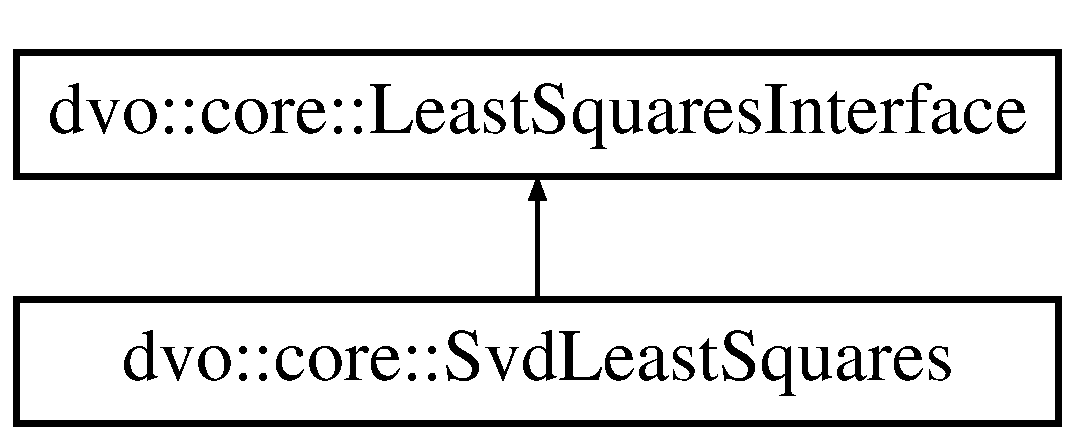
\includegraphics[height=2.000000cm]{classdvo_1_1core_1_1_svd_least_squares}
\end{center}
\end{figure}
\subsection*{Public Member Functions}
\begin{DoxyCompactItemize}
\item 
virtual \mbox{\hyperlink{classdvo_1_1core_1_1_svd_least_squares_ae60699467df2eca3f9e8cc7814388d9f}{$\sim$\+Svd\+Least\+Squares}} ()
\item 
virtual void \mbox{\hyperlink{classdvo_1_1core_1_1_svd_least_squares_aa09756d97cb63e8dc8276a88a1a07791}{initialize}} (const size\+\_\+t maxnum\+\_\+constraints)
\item 
virtual void \mbox{\hyperlink{classdvo_1_1core_1_1_svd_least_squares_ae9d28bc58804d7e43cf461ca092b9563}{update}} (const \mbox{\hyperlink{namespacedvo_1_1core_a05327f3312d32a301bce9fccda9e5807}{Vector6}} \&\mbox{\hyperlink{classdvo_1_1core_1_1_svd_least_squares_a8c0eaffdf1517bb11cb3fe7425e3274e}{J}}, const \mbox{\hyperlink{namespacedvo_1_1core_ab9c199d221775a923e2549ad7e15c323}{Num\+Type}} \&res, const \mbox{\hyperlink{namespacedvo_1_1core_ab9c199d221775a923e2549ad7e15c323}{Num\+Type}} \&weight=1.\+0f)
\item 
virtual void \mbox{\hyperlink{classdvo_1_1core_1_1_svd_least_squares_ac91cb5c82af6eb9d91d3ef4e85dc76a3}{finish}} ()
\item 
virtual void \mbox{\hyperlink{classdvo_1_1core_1_1_svd_least_squares_ae0124d7c24b90b1101bf38da59f789aa}{solve}} (\mbox{\hyperlink{namespacedvo_1_1core_a05327f3312d32a301bce9fccda9e5807}{Vector6}} \&x)
\end{DoxyCompactItemize}
\subsection*{Public Attributes}
\begin{DoxyCompactItemize}
\item 
\mbox{\hyperlink{classdvo_1_1core_1_1_svd_least_squares_a437352a5c072b985547c122d22850da6}{E\+I\+G\+E\+N\+\_\+\+M\+A\+K\+E\+\_\+\+A\+L\+I\+G\+N\+E\+D\+\_\+\+O\+P\+E\+R\+A\+T\+O\+R\+\_\+\+N\+EW}}
\item 
Eigen\+::\+Matrix$<$ \mbox{\hyperlink{namespacedvo_1_1core_ab9c199d221775a923e2549ad7e15c323}{Num\+Type}}, Eigen\+::\+Dynamic, 6 $>$ \mbox{\hyperlink{classdvo_1_1core_1_1_svd_least_squares_a8c0eaffdf1517bb11cb3fe7425e3274e}{J}}
\item 
Eigen\+::\+Matrix$<$ \mbox{\hyperlink{namespacedvo_1_1core_ab9c199d221775a923e2549ad7e15c323}{Num\+Type}}, Eigen\+::\+Dynamic, 1 $>$ \mbox{\hyperlink{classdvo_1_1core_1_1_svd_least_squares_a8f1cb060b554d4f77da3db4e7146f96b}{residuals}}
\end{DoxyCompactItemize}


\subsection{Constructor \& Destructor Documentation}
\mbox{\Hypertarget{classdvo_1_1core_1_1_svd_least_squares_ae60699467df2eca3f9e8cc7814388d9f}\label{classdvo_1_1core_1_1_svd_least_squares_ae60699467df2eca3f9e8cc7814388d9f}} 
\index{dvo\+::core\+::\+Svd\+Least\+Squares@{dvo\+::core\+::\+Svd\+Least\+Squares}!````~Svd\+Least\+Squares@{$\sim$\+Svd\+Least\+Squares}}
\index{````~Svd\+Least\+Squares@{$\sim$\+Svd\+Least\+Squares}!dvo\+::core\+::\+Svd\+Least\+Squares@{dvo\+::core\+::\+Svd\+Least\+Squares}}
\subsubsection{\texorpdfstring{$\sim$\+Svd\+Least\+Squares()}{~SvdLeastSquares()}}
{\footnotesize\ttfamily dvo\+::core\+::\+Svd\+Least\+Squares\+::$\sim$\+Svd\+Least\+Squares (\begin{DoxyParamCaption}{ }\end{DoxyParamCaption})\hspace{0.3cm}{\ttfamily [virtual]}}



\subsection{Member Function Documentation}
\mbox{\Hypertarget{classdvo_1_1core_1_1_svd_least_squares_ac91cb5c82af6eb9d91d3ef4e85dc76a3}\label{classdvo_1_1core_1_1_svd_least_squares_ac91cb5c82af6eb9d91d3ef4e85dc76a3}} 
\index{dvo\+::core\+::\+Svd\+Least\+Squares@{dvo\+::core\+::\+Svd\+Least\+Squares}!finish@{finish}}
\index{finish@{finish}!dvo\+::core\+::\+Svd\+Least\+Squares@{dvo\+::core\+::\+Svd\+Least\+Squares}}
\subsubsection{\texorpdfstring{finish()}{finish()}}
{\footnotesize\ttfamily void dvo\+::core\+::\+Svd\+Least\+Squares\+::finish (\begin{DoxyParamCaption}{ }\end{DoxyParamCaption})\hspace{0.3cm}{\ttfamily [virtual]}}



Implements \mbox{\hyperlink{classdvo_1_1core_1_1_least_squares_interface_a2e580a70e96f0e7d6d70f6047891a42a}{dvo\+::core\+::\+Least\+Squares\+Interface}}.

\mbox{\Hypertarget{classdvo_1_1core_1_1_svd_least_squares_aa09756d97cb63e8dc8276a88a1a07791}\label{classdvo_1_1core_1_1_svd_least_squares_aa09756d97cb63e8dc8276a88a1a07791}} 
\index{dvo\+::core\+::\+Svd\+Least\+Squares@{dvo\+::core\+::\+Svd\+Least\+Squares}!initialize@{initialize}}
\index{initialize@{initialize}!dvo\+::core\+::\+Svd\+Least\+Squares@{dvo\+::core\+::\+Svd\+Least\+Squares}}
\subsubsection{\texorpdfstring{initialize()}{initialize()}}
{\footnotesize\ttfamily void dvo\+::core\+::\+Svd\+Least\+Squares\+::initialize (\begin{DoxyParamCaption}\item[{const size\+\_\+t}]{maxnum\+\_\+constraints }\end{DoxyParamCaption})\hspace{0.3cm}{\ttfamily [virtual]}}



Implements \mbox{\hyperlink{classdvo_1_1core_1_1_least_squares_interface_a09e5784f74d7352a9550a8aa523d30d7}{dvo\+::core\+::\+Least\+Squares\+Interface}}.

\mbox{\Hypertarget{classdvo_1_1core_1_1_svd_least_squares_ae0124d7c24b90b1101bf38da59f789aa}\label{classdvo_1_1core_1_1_svd_least_squares_ae0124d7c24b90b1101bf38da59f789aa}} 
\index{dvo\+::core\+::\+Svd\+Least\+Squares@{dvo\+::core\+::\+Svd\+Least\+Squares}!solve@{solve}}
\index{solve@{solve}!dvo\+::core\+::\+Svd\+Least\+Squares@{dvo\+::core\+::\+Svd\+Least\+Squares}}
\subsubsection{\texorpdfstring{solve()}{solve()}}
{\footnotesize\ttfamily void dvo\+::core\+::\+Svd\+Least\+Squares\+::solve (\begin{DoxyParamCaption}\item[{\mbox{\hyperlink{namespacedvo_1_1core_a05327f3312d32a301bce9fccda9e5807}{Vector6}} \&}]{x }\end{DoxyParamCaption})\hspace{0.3cm}{\ttfamily [virtual]}}



Implements \mbox{\hyperlink{classdvo_1_1core_1_1_least_squares_interface_a3e2b3c894c5286fdee79316e6fa4d691}{dvo\+::core\+::\+Least\+Squares\+Interface}}.

\mbox{\Hypertarget{classdvo_1_1core_1_1_svd_least_squares_ae9d28bc58804d7e43cf461ca092b9563}\label{classdvo_1_1core_1_1_svd_least_squares_ae9d28bc58804d7e43cf461ca092b9563}} 
\index{dvo\+::core\+::\+Svd\+Least\+Squares@{dvo\+::core\+::\+Svd\+Least\+Squares}!update@{update}}
\index{update@{update}!dvo\+::core\+::\+Svd\+Least\+Squares@{dvo\+::core\+::\+Svd\+Least\+Squares}}
\subsubsection{\texorpdfstring{update()}{update()}}
{\footnotesize\ttfamily void dvo\+::core\+::\+Svd\+Least\+Squares\+::update (\begin{DoxyParamCaption}\item[{const \mbox{\hyperlink{namespacedvo_1_1core_a05327f3312d32a301bce9fccda9e5807}{Vector6}} \&}]{J,  }\item[{const \mbox{\hyperlink{namespacedvo_1_1core_ab9c199d221775a923e2549ad7e15c323}{Num\+Type}} \&}]{res,  }\item[{const \mbox{\hyperlink{namespacedvo_1_1core_ab9c199d221775a923e2549ad7e15c323}{Num\+Type}} \&}]{weight = {\ttfamily 1.0f} }\end{DoxyParamCaption})\hspace{0.3cm}{\ttfamily [virtual]}}



Implements \mbox{\hyperlink{classdvo_1_1core_1_1_least_squares_interface_a5f5cc1c312a01ff4e7ca91e90a73ccf3}{dvo\+::core\+::\+Least\+Squares\+Interface}}.



\subsection{Member Data Documentation}
\mbox{\Hypertarget{classdvo_1_1core_1_1_svd_least_squares_a437352a5c072b985547c122d22850da6}\label{classdvo_1_1core_1_1_svd_least_squares_a437352a5c072b985547c122d22850da6}} 
\index{dvo\+::core\+::\+Svd\+Least\+Squares@{dvo\+::core\+::\+Svd\+Least\+Squares}!E\+I\+G\+E\+N\+\_\+\+M\+A\+K\+E\+\_\+\+A\+L\+I\+G\+N\+E\+D\+\_\+\+O\+P\+E\+R\+A\+T\+O\+R\+\_\+\+N\+EW@{E\+I\+G\+E\+N\+\_\+\+M\+A\+K\+E\+\_\+\+A\+L\+I\+G\+N\+E\+D\+\_\+\+O\+P\+E\+R\+A\+T\+O\+R\+\_\+\+N\+EW}}
\index{E\+I\+G\+E\+N\+\_\+\+M\+A\+K\+E\+\_\+\+A\+L\+I\+G\+N\+E\+D\+\_\+\+O\+P\+E\+R\+A\+T\+O\+R\+\_\+\+N\+EW@{E\+I\+G\+E\+N\+\_\+\+M\+A\+K\+E\+\_\+\+A\+L\+I\+G\+N\+E\+D\+\_\+\+O\+P\+E\+R\+A\+T\+O\+R\+\_\+\+N\+EW}!dvo\+::core\+::\+Svd\+Least\+Squares@{dvo\+::core\+::\+Svd\+Least\+Squares}}
\subsubsection{\texorpdfstring{E\+I\+G\+E\+N\+\_\+\+M\+A\+K\+E\+\_\+\+A\+L\+I\+G\+N\+E\+D\+\_\+\+O\+P\+E\+R\+A\+T\+O\+R\+\_\+\+N\+EW}{EIGEN\_MAKE\_ALIGNED\_OPERATOR\_NEW}}
{\footnotesize\ttfamily dvo\+::core\+::\+Svd\+Least\+Squares\+::\+E\+I\+G\+E\+N\+\_\+\+M\+A\+K\+E\+\_\+\+A\+L\+I\+G\+N\+E\+D\+\_\+\+O\+P\+E\+R\+A\+T\+O\+R\+\_\+\+N\+EW}

\mbox{\Hypertarget{classdvo_1_1core_1_1_svd_least_squares_a8c0eaffdf1517bb11cb3fe7425e3274e}\label{classdvo_1_1core_1_1_svd_least_squares_a8c0eaffdf1517bb11cb3fe7425e3274e}} 
\index{dvo\+::core\+::\+Svd\+Least\+Squares@{dvo\+::core\+::\+Svd\+Least\+Squares}!J@{J}}
\index{J@{J}!dvo\+::core\+::\+Svd\+Least\+Squares@{dvo\+::core\+::\+Svd\+Least\+Squares}}
\subsubsection{\texorpdfstring{J}{J}}
{\footnotesize\ttfamily Eigen\+::\+Matrix$<$\mbox{\hyperlink{namespacedvo_1_1core_ab9c199d221775a923e2549ad7e15c323}{Num\+Type}}, Eigen\+::\+Dynamic, 6$>$ dvo\+::core\+::\+Svd\+Least\+Squares\+::J}

\mbox{\Hypertarget{classdvo_1_1core_1_1_svd_least_squares_a8f1cb060b554d4f77da3db4e7146f96b}\label{classdvo_1_1core_1_1_svd_least_squares_a8f1cb060b554d4f77da3db4e7146f96b}} 
\index{dvo\+::core\+::\+Svd\+Least\+Squares@{dvo\+::core\+::\+Svd\+Least\+Squares}!residuals@{residuals}}
\index{residuals@{residuals}!dvo\+::core\+::\+Svd\+Least\+Squares@{dvo\+::core\+::\+Svd\+Least\+Squares}}
\subsubsection{\texorpdfstring{residuals}{residuals}}
{\footnotesize\ttfamily Eigen\+::\+Matrix$<$\mbox{\hyperlink{namespacedvo_1_1core_ab9c199d221775a923e2549ad7e15c323}{Num\+Type}}, Eigen\+::\+Dynamic, 1$>$ dvo\+::core\+::\+Svd\+Least\+Squares\+::residuals}



The documentation for this class was generated from the following files\+:\begin{DoxyCompactItemize}
\item 
dvo\+\_\+core/include/dvo/core/\mbox{\hyperlink{least__squares_8h}{least\+\_\+squares.\+h}}\item 
dvo\+\_\+core/src/core/\mbox{\hyperlink{least__squares_8cpp}{least\+\_\+squares.\+cpp}}\end{DoxyCompactItemize}

\hypertarget{structdvo_1_1visualization_1_1_switch}{}\section{dvo\+:\+:visualization\+:\+:Switch Struct Reference}
\label{structdvo_1_1visualization_1_1_switch}\index{dvo\+::visualization\+::\+Switch@{dvo\+::visualization\+::\+Switch}}


{\ttfamily \#include $<$pcl\+\_\+camera\+\_\+trajectory\+\_\+visualizer.\+h$>$}

\subsection*{Public Member Functions}
\begin{DoxyCompactItemize}
\item 
\mbox{\hyperlink{structdvo_1_1visualization_1_1_switch_a4d601eeee9e3b30de1ebc22c42aa5102}{Switch}} (bool initial)
\item 
void \mbox{\hyperlink{structdvo_1_1visualization_1_1_switch_af618d5fd5a327abf0873defe1532a2c3}{toggle}} ()
\item 
bool \mbox{\hyperlink{structdvo_1_1visualization_1_1_switch_ab4e0d6e3033221e4d052ac0b89b118d1}{value}} () const
\item 
bool \mbox{\hyperlink{structdvo_1_1visualization_1_1_switch_a2c81c1498c9d450c6e8aae1173045954}{changed}} ()
\end{DoxyCompactItemize}


\subsection{Constructor \& Destructor Documentation}
\mbox{\Hypertarget{structdvo_1_1visualization_1_1_switch_a4d601eeee9e3b30de1ebc22c42aa5102}\label{structdvo_1_1visualization_1_1_switch_a4d601eeee9e3b30de1ebc22c42aa5102}} 
\index{dvo\+::visualization\+::\+Switch@{dvo\+::visualization\+::\+Switch}!Switch@{Switch}}
\index{Switch@{Switch}!dvo\+::visualization\+::\+Switch@{dvo\+::visualization\+::\+Switch}}
\subsubsection{\texorpdfstring{Switch()}{Switch()}}
{\footnotesize\ttfamily dvo\+::visualization\+::\+Switch\+::\+Switch (\begin{DoxyParamCaption}\item[{bool}]{initial }\end{DoxyParamCaption})\hspace{0.3cm}{\ttfamily [inline]}}



\subsection{Member Function Documentation}
\mbox{\Hypertarget{structdvo_1_1visualization_1_1_switch_a2c81c1498c9d450c6e8aae1173045954}\label{structdvo_1_1visualization_1_1_switch_a2c81c1498c9d450c6e8aae1173045954}} 
\index{dvo\+::visualization\+::\+Switch@{dvo\+::visualization\+::\+Switch}!changed@{changed}}
\index{changed@{changed}!dvo\+::visualization\+::\+Switch@{dvo\+::visualization\+::\+Switch}}
\subsubsection{\texorpdfstring{changed()}{changed()}}
{\footnotesize\ttfamily bool dvo\+::visualization\+::\+Switch\+::changed (\begin{DoxyParamCaption}{ }\end{DoxyParamCaption})\hspace{0.3cm}{\ttfamily [inline]}}

\mbox{\Hypertarget{structdvo_1_1visualization_1_1_switch_af618d5fd5a327abf0873defe1532a2c3}\label{structdvo_1_1visualization_1_1_switch_af618d5fd5a327abf0873defe1532a2c3}} 
\index{dvo\+::visualization\+::\+Switch@{dvo\+::visualization\+::\+Switch}!toggle@{toggle}}
\index{toggle@{toggle}!dvo\+::visualization\+::\+Switch@{dvo\+::visualization\+::\+Switch}}
\subsubsection{\texorpdfstring{toggle()}{toggle()}}
{\footnotesize\ttfamily void dvo\+::visualization\+::\+Switch\+::toggle (\begin{DoxyParamCaption}{ }\end{DoxyParamCaption})\hspace{0.3cm}{\ttfamily [inline]}}

\mbox{\Hypertarget{structdvo_1_1visualization_1_1_switch_ab4e0d6e3033221e4d052ac0b89b118d1}\label{structdvo_1_1visualization_1_1_switch_ab4e0d6e3033221e4d052ac0b89b118d1}} 
\index{dvo\+::visualization\+::\+Switch@{dvo\+::visualization\+::\+Switch}!value@{value}}
\index{value@{value}!dvo\+::visualization\+::\+Switch@{dvo\+::visualization\+::\+Switch}}
\subsubsection{\texorpdfstring{value()}{value()}}
{\footnotesize\ttfamily bool dvo\+::visualization\+::\+Switch\+::value (\begin{DoxyParamCaption}{ }\end{DoxyParamCaption}) const\hspace{0.3cm}{\ttfamily [inline]}}



The documentation for this struct was generated from the following file\+:\begin{DoxyCompactItemize}
\item 
dvo\+\_\+core/include/dvo/visualization/\mbox{\hyperlink{pcl__camera__trajectory__visualizer_8h}{pcl\+\_\+camera\+\_\+trajectory\+\_\+visualizer.\+h}}\end{DoxyCompactItemize}

\hypertarget{classdvo_1_1core_1_1_t_distribution_influence_function}{}\section{dvo\+:\+:core\+:\+:T\+Distribution\+Influence\+Function Class Reference}
\label{classdvo_1_1core_1_1_t_distribution_influence_function}\index{dvo\+::core\+::\+T\+Distribution\+Influence\+Function@{dvo\+::core\+::\+T\+Distribution\+Influence\+Function}}


{\ttfamily \#include $<$weight\+\_\+calculation.\+h$>$}

Inheritance diagram for dvo\+:\+:core\+:\+:T\+Distribution\+Influence\+Function\+:\begin{figure}[H]
\begin{center}
\leavevmode
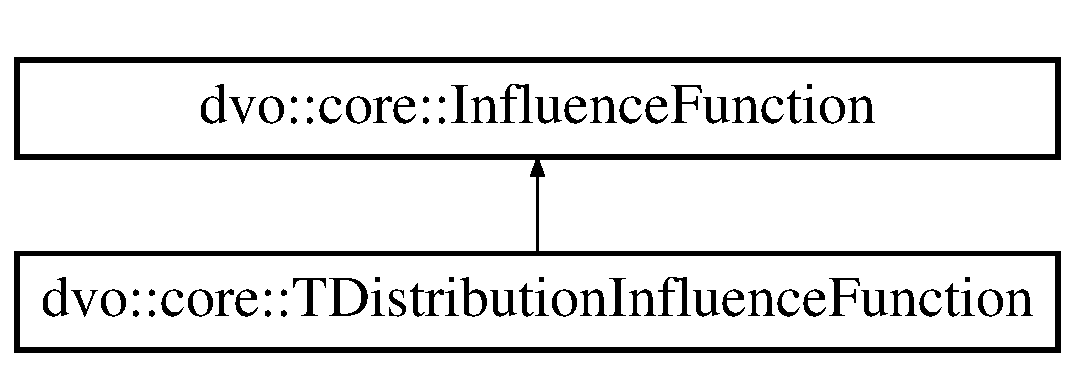
\includegraphics[height=2.000000cm]{classdvo_1_1core_1_1_t_distribution_influence_function}
\end{center}
\end{figure}
\subsection*{Public Member Functions}
\begin{DoxyCompactItemize}
\item 
\mbox{\hyperlink{classdvo_1_1core_1_1_t_distribution_influence_function_ae58bd8035bc312c717b041d9dce81d48}{T\+Distribution\+Influence\+Function}} (const float dof=\mbox{\hyperlink{classdvo_1_1core_1_1_t_distribution_influence_function_a7a64badce04fe13458febb2371d216dd}{D\+E\+F\+A\+U\+L\+T\+\_\+\+D\+OF}})
\item 
virtual \mbox{\hyperlink{classdvo_1_1core_1_1_t_distribution_influence_function_a60d61b5e830b73bb6ab223abb2705def}{$\sim$\+T\+Distribution\+Influence\+Function}} ()
\item 
virtual float \mbox{\hyperlink{classdvo_1_1core_1_1_t_distribution_influence_function_a3210e7ab6f57975751e75845d3d22598}{value}} (const float \&x) const
\item 
virtual void \mbox{\hyperlink{classdvo_1_1core_1_1_t_distribution_influence_function_ad9030e81f013c14015c3ad97a2f821be}{configure}} (const float \&param)
\end{DoxyCompactItemize}
\subsection*{Static Public Attributes}
\begin{DoxyCompactItemize}
\item 
static const float \mbox{\hyperlink{classdvo_1_1core_1_1_t_distribution_influence_function_a7a64badce04fe13458febb2371d216dd}{D\+E\+F\+A\+U\+L\+T\+\_\+\+D\+OF}} = 5.\+0f
\end{DoxyCompactItemize}


\subsection{Constructor \& Destructor Documentation}
\mbox{\Hypertarget{classdvo_1_1core_1_1_t_distribution_influence_function_ae58bd8035bc312c717b041d9dce81d48}\label{classdvo_1_1core_1_1_t_distribution_influence_function_ae58bd8035bc312c717b041d9dce81d48}} 
\index{dvo\+::core\+::\+T\+Distribution\+Influence\+Function@{dvo\+::core\+::\+T\+Distribution\+Influence\+Function}!T\+Distribution\+Influence\+Function@{T\+Distribution\+Influence\+Function}}
\index{T\+Distribution\+Influence\+Function@{T\+Distribution\+Influence\+Function}!dvo\+::core\+::\+T\+Distribution\+Influence\+Function@{dvo\+::core\+::\+T\+Distribution\+Influence\+Function}}
\subsubsection{\texorpdfstring{T\+Distribution\+Influence\+Function()}{TDistributionInfluenceFunction()}}
{\footnotesize\ttfamily dvo\+::core\+::\+T\+Distribution\+Influence\+Function\+::\+T\+Distribution\+Influence\+Function (\begin{DoxyParamCaption}\item[{const float}]{dof = {\ttfamily \mbox{\hyperlink{classdvo_1_1core_1_1_t_distribution_influence_function_a7a64badce04fe13458febb2371d216dd}{D\+E\+F\+A\+U\+L\+T\+\_\+\+D\+OF}}} }\end{DoxyParamCaption})}

\mbox{\Hypertarget{classdvo_1_1core_1_1_t_distribution_influence_function_a60d61b5e830b73bb6ab223abb2705def}\label{classdvo_1_1core_1_1_t_distribution_influence_function_a60d61b5e830b73bb6ab223abb2705def}} 
\index{dvo\+::core\+::\+T\+Distribution\+Influence\+Function@{dvo\+::core\+::\+T\+Distribution\+Influence\+Function}!````~T\+Distribution\+Influence\+Function@{$\sim$\+T\+Distribution\+Influence\+Function}}
\index{````~T\+Distribution\+Influence\+Function@{$\sim$\+T\+Distribution\+Influence\+Function}!dvo\+::core\+::\+T\+Distribution\+Influence\+Function@{dvo\+::core\+::\+T\+Distribution\+Influence\+Function}}
\subsubsection{\texorpdfstring{$\sim$\+T\+Distribution\+Influence\+Function()}{~TDistributionInfluenceFunction()}}
{\footnotesize\ttfamily virtual dvo\+::core\+::\+T\+Distribution\+Influence\+Function\+::$\sim$\+T\+Distribution\+Influence\+Function (\begin{DoxyParamCaption}{ }\end{DoxyParamCaption})\hspace{0.3cm}{\ttfamily [inline]}, {\ttfamily [virtual]}}



\subsection{Member Function Documentation}
\mbox{\Hypertarget{classdvo_1_1core_1_1_t_distribution_influence_function_ad9030e81f013c14015c3ad97a2f821be}\label{classdvo_1_1core_1_1_t_distribution_influence_function_ad9030e81f013c14015c3ad97a2f821be}} 
\index{dvo\+::core\+::\+T\+Distribution\+Influence\+Function@{dvo\+::core\+::\+T\+Distribution\+Influence\+Function}!configure@{configure}}
\index{configure@{configure}!dvo\+::core\+::\+T\+Distribution\+Influence\+Function@{dvo\+::core\+::\+T\+Distribution\+Influence\+Function}}
\subsubsection{\texorpdfstring{configure()}{configure()}}
{\footnotesize\ttfamily void dvo\+::core\+::\+T\+Distribution\+Influence\+Function\+::configure (\begin{DoxyParamCaption}\item[{const float \&}]{param }\end{DoxyParamCaption})\hspace{0.3cm}{\ttfamily [virtual]}}



Reimplemented from \mbox{\hyperlink{classdvo_1_1core_1_1_influence_function_a4773b03ca609bc5d8391d09d92ab34ad}{dvo\+::core\+::\+Influence\+Function}}.

\mbox{\Hypertarget{classdvo_1_1core_1_1_t_distribution_influence_function_a3210e7ab6f57975751e75845d3d22598}\label{classdvo_1_1core_1_1_t_distribution_influence_function_a3210e7ab6f57975751e75845d3d22598}} 
\index{dvo\+::core\+::\+T\+Distribution\+Influence\+Function@{dvo\+::core\+::\+T\+Distribution\+Influence\+Function}!value@{value}}
\index{value@{value}!dvo\+::core\+::\+T\+Distribution\+Influence\+Function@{dvo\+::core\+::\+T\+Distribution\+Influence\+Function}}
\subsubsection{\texorpdfstring{value()}{value()}}
{\footnotesize\ttfamily float dvo\+::core\+::\+T\+Distribution\+Influence\+Function\+::value (\begin{DoxyParamCaption}\item[{const float \&}]{x }\end{DoxyParamCaption}) const\hspace{0.3cm}{\ttfamily [inline]}, {\ttfamily [virtual]}}



Implements \mbox{\hyperlink{classdvo_1_1core_1_1_influence_function_a158082c763fa9de460e75a285bb91f1e}{dvo\+::core\+::\+Influence\+Function}}.



\subsection{Member Data Documentation}
\mbox{\Hypertarget{classdvo_1_1core_1_1_t_distribution_influence_function_a7a64badce04fe13458febb2371d216dd}\label{classdvo_1_1core_1_1_t_distribution_influence_function_a7a64badce04fe13458febb2371d216dd}} 
\index{dvo\+::core\+::\+T\+Distribution\+Influence\+Function@{dvo\+::core\+::\+T\+Distribution\+Influence\+Function}!D\+E\+F\+A\+U\+L\+T\+\_\+\+D\+OF@{D\+E\+F\+A\+U\+L\+T\+\_\+\+D\+OF}}
\index{D\+E\+F\+A\+U\+L\+T\+\_\+\+D\+OF@{D\+E\+F\+A\+U\+L\+T\+\_\+\+D\+OF}!dvo\+::core\+::\+T\+Distribution\+Influence\+Function@{dvo\+::core\+::\+T\+Distribution\+Influence\+Function}}
\subsubsection{\texorpdfstring{D\+E\+F\+A\+U\+L\+T\+\_\+\+D\+OF}{DEFAULT\_DOF}}
{\footnotesize\ttfamily const float dvo\+::core\+::\+T\+Distribution\+Influence\+Function\+::\+D\+E\+F\+A\+U\+L\+T\+\_\+\+D\+OF = 5.\+0f\hspace{0.3cm}{\ttfamily [static]}}



The documentation for this class was generated from the following files\+:\begin{DoxyCompactItemize}
\item 
dvo\+\_\+core/include/dvo/core/\mbox{\hyperlink{weight__calculation_8h}{weight\+\_\+calculation.\+h}}\item 
dvo\+\_\+core/src/core/\mbox{\hyperlink{weight__calculation_8cpp}{weight\+\_\+calculation.\+cpp}}\end{DoxyCompactItemize}

\hypertarget{classdvo_1_1core_1_1_t_distribution_scale_estimator}{}\section{dvo\+:\+:core\+:\+:T\+Distribution\+Scale\+Estimator Class Reference}
\label{classdvo_1_1core_1_1_t_distribution_scale_estimator}\index{dvo\+::core\+::\+T\+Distribution\+Scale\+Estimator@{dvo\+::core\+::\+T\+Distribution\+Scale\+Estimator}}


{\ttfamily \#include $<$weight\+\_\+calculation.\+h$>$}

Inheritance diagram for dvo\+:\+:core\+:\+:T\+Distribution\+Scale\+Estimator\+:\begin{figure}[H]
\begin{center}
\leavevmode
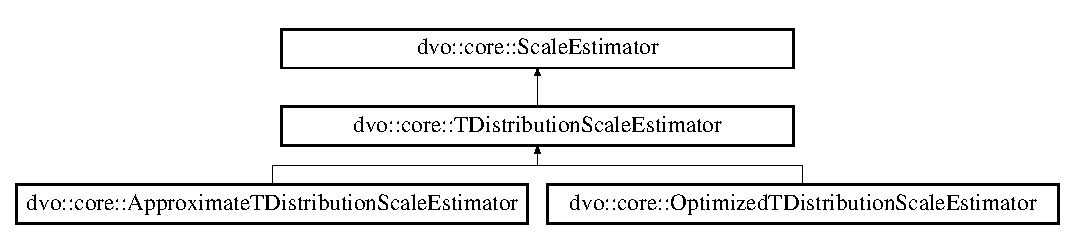
\includegraphics[height=2.781457cm]{classdvo_1_1core_1_1_t_distribution_scale_estimator}
\end{center}
\end{figure}
\subsection*{Public Member Functions}
\begin{DoxyCompactItemize}
\item 
\mbox{\hyperlink{classdvo_1_1core_1_1_t_distribution_scale_estimator_a1b50430701a4f6c103dedf40102e6506}{T\+Distribution\+Scale\+Estimator}} (const float \mbox{\hyperlink{classdvo_1_1core_1_1_t_distribution_scale_estimator_a4c5ece510a3315bad7ca711a27466eb9}{dof}}=\mbox{\hyperlink{classdvo_1_1core_1_1_t_distribution_scale_estimator_a031ff291023c516c23bce04b34b79957}{D\+E\+F\+A\+U\+L\+T\+\_\+\+D\+OF}})
\item 
virtual \mbox{\hyperlink{classdvo_1_1core_1_1_t_distribution_scale_estimator_ae96b7b80f30e797a21f59f60cce22a3c}{$\sim$\+T\+Distribution\+Scale\+Estimator}} ()
\item 
virtual float \mbox{\hyperlink{classdvo_1_1core_1_1_t_distribution_scale_estimator_a0ed88ffeb9b71110e3ae69b681526bc4}{compute}} (const cv\+::\+Mat \&errors) const
\item 
virtual void \mbox{\hyperlink{classdvo_1_1core_1_1_t_distribution_scale_estimator_a34ec79e7811c148606817510a00aa585}{configure}} (const float \&param)
\end{DoxyCompactItemize}
\subsection*{Static Public Attributes}
\begin{DoxyCompactItemize}
\item 
static const float \mbox{\hyperlink{classdvo_1_1core_1_1_t_distribution_scale_estimator_a031ff291023c516c23bce04b34b79957}{D\+E\+F\+A\+U\+L\+T\+\_\+\+D\+OF}} = 5.\+0f
\item 
static const float \mbox{\hyperlink{classdvo_1_1core_1_1_t_distribution_scale_estimator_a536ae191c3a6827914ecc22308ff87b7}{I\+N\+I\+T\+I\+A\+L\+\_\+\+S\+I\+G\+MA}} = 5.\+0f
\end{DoxyCompactItemize}
\subsection*{Protected Attributes}
\begin{DoxyCompactItemize}
\item 
float \mbox{\hyperlink{classdvo_1_1core_1_1_t_distribution_scale_estimator_a4c5ece510a3315bad7ca711a27466eb9}{dof}}
\item 
float \mbox{\hyperlink{classdvo_1_1core_1_1_t_distribution_scale_estimator_ab2b25d1856c4e51dfeeb1abd9aafbcb7}{initial\+\_\+sigma}}
\end{DoxyCompactItemize}


\subsection{Constructor \& Destructor Documentation}
\mbox{\Hypertarget{classdvo_1_1core_1_1_t_distribution_scale_estimator_a1b50430701a4f6c103dedf40102e6506}\label{classdvo_1_1core_1_1_t_distribution_scale_estimator_a1b50430701a4f6c103dedf40102e6506}} 
\index{dvo\+::core\+::\+T\+Distribution\+Scale\+Estimator@{dvo\+::core\+::\+T\+Distribution\+Scale\+Estimator}!T\+Distribution\+Scale\+Estimator@{T\+Distribution\+Scale\+Estimator}}
\index{T\+Distribution\+Scale\+Estimator@{T\+Distribution\+Scale\+Estimator}!dvo\+::core\+::\+T\+Distribution\+Scale\+Estimator@{dvo\+::core\+::\+T\+Distribution\+Scale\+Estimator}}
\subsubsection{\texorpdfstring{T\+Distribution\+Scale\+Estimator()}{TDistributionScaleEstimator()}}
{\footnotesize\ttfamily dvo\+::core\+::\+T\+Distribution\+Scale\+Estimator\+::\+T\+Distribution\+Scale\+Estimator (\begin{DoxyParamCaption}\item[{const float}]{dof = {\ttfamily \mbox{\hyperlink{classdvo_1_1core_1_1_t_distribution_scale_estimator_a031ff291023c516c23bce04b34b79957}{D\+E\+F\+A\+U\+L\+T\+\_\+\+D\+OF}}} }\end{DoxyParamCaption})}

\mbox{\Hypertarget{classdvo_1_1core_1_1_t_distribution_scale_estimator_ae96b7b80f30e797a21f59f60cce22a3c}\label{classdvo_1_1core_1_1_t_distribution_scale_estimator_ae96b7b80f30e797a21f59f60cce22a3c}} 
\index{dvo\+::core\+::\+T\+Distribution\+Scale\+Estimator@{dvo\+::core\+::\+T\+Distribution\+Scale\+Estimator}!````~T\+Distribution\+Scale\+Estimator@{$\sim$\+T\+Distribution\+Scale\+Estimator}}
\index{````~T\+Distribution\+Scale\+Estimator@{$\sim$\+T\+Distribution\+Scale\+Estimator}!dvo\+::core\+::\+T\+Distribution\+Scale\+Estimator@{dvo\+::core\+::\+T\+Distribution\+Scale\+Estimator}}
\subsubsection{\texorpdfstring{$\sim$\+T\+Distribution\+Scale\+Estimator()}{~TDistributionScaleEstimator()}}
{\footnotesize\ttfamily virtual dvo\+::core\+::\+T\+Distribution\+Scale\+Estimator\+::$\sim$\+T\+Distribution\+Scale\+Estimator (\begin{DoxyParamCaption}{ }\end{DoxyParamCaption})\hspace{0.3cm}{\ttfamily [inline]}, {\ttfamily [virtual]}}



\subsection{Member Function Documentation}
\mbox{\Hypertarget{classdvo_1_1core_1_1_t_distribution_scale_estimator_a0ed88ffeb9b71110e3ae69b681526bc4}\label{classdvo_1_1core_1_1_t_distribution_scale_estimator_a0ed88ffeb9b71110e3ae69b681526bc4}} 
\index{dvo\+::core\+::\+T\+Distribution\+Scale\+Estimator@{dvo\+::core\+::\+T\+Distribution\+Scale\+Estimator}!compute@{compute}}
\index{compute@{compute}!dvo\+::core\+::\+T\+Distribution\+Scale\+Estimator@{dvo\+::core\+::\+T\+Distribution\+Scale\+Estimator}}
\subsubsection{\texorpdfstring{compute()}{compute()}}
{\footnotesize\ttfamily float dvo\+::core\+::\+T\+Distribution\+Scale\+Estimator\+::compute (\begin{DoxyParamCaption}\item[{const cv\+::\+Mat \&}]{errors }\end{DoxyParamCaption}) const\hspace{0.3cm}{\ttfamily [virtual]}}



Implements \mbox{\hyperlink{classdvo_1_1core_1_1_scale_estimator_a6968ac2cd37c2ce1c966f0c9e17d1a3c}{dvo\+::core\+::\+Scale\+Estimator}}.



Reimplemented in \mbox{\hyperlink{classdvo_1_1core_1_1_approximate_t_distribution_scale_estimator_aee2b37700df1eb0125b8e0d352f7ceab}{dvo\+::core\+::\+Approximate\+T\+Distribution\+Scale\+Estimator}}, and \mbox{\hyperlink{classdvo_1_1core_1_1_optimized_t_distribution_scale_estimator_ace9304a785bd16a6ef5cf4a52f3c6299}{dvo\+::core\+::\+Optimized\+T\+Distribution\+Scale\+Estimator}}.

\mbox{\Hypertarget{classdvo_1_1core_1_1_t_distribution_scale_estimator_a34ec79e7811c148606817510a00aa585}\label{classdvo_1_1core_1_1_t_distribution_scale_estimator_a34ec79e7811c148606817510a00aa585}} 
\index{dvo\+::core\+::\+T\+Distribution\+Scale\+Estimator@{dvo\+::core\+::\+T\+Distribution\+Scale\+Estimator}!configure@{configure}}
\index{configure@{configure}!dvo\+::core\+::\+T\+Distribution\+Scale\+Estimator@{dvo\+::core\+::\+T\+Distribution\+Scale\+Estimator}}
\subsubsection{\texorpdfstring{configure()}{configure()}}
{\footnotesize\ttfamily void dvo\+::core\+::\+T\+Distribution\+Scale\+Estimator\+::configure (\begin{DoxyParamCaption}\item[{const float \&}]{param }\end{DoxyParamCaption})\hspace{0.3cm}{\ttfamily [virtual]}}



Reimplemented from \mbox{\hyperlink{classdvo_1_1core_1_1_scale_estimator_a58b5d7926b08e85e7393436156f3ef43}{dvo\+::core\+::\+Scale\+Estimator}}.



\subsection{Member Data Documentation}
\mbox{\Hypertarget{classdvo_1_1core_1_1_t_distribution_scale_estimator_a031ff291023c516c23bce04b34b79957}\label{classdvo_1_1core_1_1_t_distribution_scale_estimator_a031ff291023c516c23bce04b34b79957}} 
\index{dvo\+::core\+::\+T\+Distribution\+Scale\+Estimator@{dvo\+::core\+::\+T\+Distribution\+Scale\+Estimator}!D\+E\+F\+A\+U\+L\+T\+\_\+\+D\+OF@{D\+E\+F\+A\+U\+L\+T\+\_\+\+D\+OF}}
\index{D\+E\+F\+A\+U\+L\+T\+\_\+\+D\+OF@{D\+E\+F\+A\+U\+L\+T\+\_\+\+D\+OF}!dvo\+::core\+::\+T\+Distribution\+Scale\+Estimator@{dvo\+::core\+::\+T\+Distribution\+Scale\+Estimator}}
\subsubsection{\texorpdfstring{D\+E\+F\+A\+U\+L\+T\+\_\+\+D\+OF}{DEFAULT\_DOF}}
{\footnotesize\ttfamily const float dvo\+::core\+::\+T\+Distribution\+Scale\+Estimator\+::\+D\+E\+F\+A\+U\+L\+T\+\_\+\+D\+OF = 5.\+0f\hspace{0.3cm}{\ttfamily [static]}}

\mbox{\Hypertarget{classdvo_1_1core_1_1_t_distribution_scale_estimator_a4c5ece510a3315bad7ca711a27466eb9}\label{classdvo_1_1core_1_1_t_distribution_scale_estimator_a4c5ece510a3315bad7ca711a27466eb9}} 
\index{dvo\+::core\+::\+T\+Distribution\+Scale\+Estimator@{dvo\+::core\+::\+T\+Distribution\+Scale\+Estimator}!dof@{dof}}
\index{dof@{dof}!dvo\+::core\+::\+T\+Distribution\+Scale\+Estimator@{dvo\+::core\+::\+T\+Distribution\+Scale\+Estimator}}
\subsubsection{\texorpdfstring{dof}{dof}}
{\footnotesize\ttfamily float dvo\+::core\+::\+T\+Distribution\+Scale\+Estimator\+::dof\hspace{0.3cm}{\ttfamily [protected]}}

\mbox{\Hypertarget{classdvo_1_1core_1_1_t_distribution_scale_estimator_a536ae191c3a6827914ecc22308ff87b7}\label{classdvo_1_1core_1_1_t_distribution_scale_estimator_a536ae191c3a6827914ecc22308ff87b7}} 
\index{dvo\+::core\+::\+T\+Distribution\+Scale\+Estimator@{dvo\+::core\+::\+T\+Distribution\+Scale\+Estimator}!I\+N\+I\+T\+I\+A\+L\+\_\+\+S\+I\+G\+MA@{I\+N\+I\+T\+I\+A\+L\+\_\+\+S\+I\+G\+MA}}
\index{I\+N\+I\+T\+I\+A\+L\+\_\+\+S\+I\+G\+MA@{I\+N\+I\+T\+I\+A\+L\+\_\+\+S\+I\+G\+MA}!dvo\+::core\+::\+T\+Distribution\+Scale\+Estimator@{dvo\+::core\+::\+T\+Distribution\+Scale\+Estimator}}
\subsubsection{\texorpdfstring{I\+N\+I\+T\+I\+A\+L\+\_\+\+S\+I\+G\+MA}{INITIAL\_SIGMA}}
{\footnotesize\ttfamily const float dvo\+::core\+::\+T\+Distribution\+Scale\+Estimator\+::\+I\+N\+I\+T\+I\+A\+L\+\_\+\+S\+I\+G\+MA = 5.\+0f\hspace{0.3cm}{\ttfamily [static]}}

\mbox{\Hypertarget{classdvo_1_1core_1_1_t_distribution_scale_estimator_ab2b25d1856c4e51dfeeb1abd9aafbcb7}\label{classdvo_1_1core_1_1_t_distribution_scale_estimator_ab2b25d1856c4e51dfeeb1abd9aafbcb7}} 
\index{dvo\+::core\+::\+T\+Distribution\+Scale\+Estimator@{dvo\+::core\+::\+T\+Distribution\+Scale\+Estimator}!initial\+\_\+sigma@{initial\+\_\+sigma}}
\index{initial\+\_\+sigma@{initial\+\_\+sigma}!dvo\+::core\+::\+T\+Distribution\+Scale\+Estimator@{dvo\+::core\+::\+T\+Distribution\+Scale\+Estimator}}
\subsubsection{\texorpdfstring{initial\+\_\+sigma}{initial\_sigma}}
{\footnotesize\ttfamily float dvo\+::core\+::\+T\+Distribution\+Scale\+Estimator\+::initial\+\_\+sigma\hspace{0.3cm}{\ttfamily [protected]}}



The documentation for this class was generated from the following files\+:\begin{DoxyCompactItemize}
\item 
dvo\+\_\+core/include/dvo/core/\mbox{\hyperlink{weight__calculation_8h}{weight\+\_\+calculation.\+h}}\item 
dvo\+\_\+core/src/core/\mbox{\hyperlink{weight__calculation_8cpp}{weight\+\_\+calculation.\+cpp}}\end{DoxyCompactItemize}

\hypertarget{structdvo_1_1core_1_1_t_distribution_scale_reduction}{}\section{dvo\+:\+:core\+:\+:T\+Distribution\+Scale\+Reduction Struct Reference}
\label{structdvo_1_1core_1_1_t_distribution_scale_reduction}\index{dvo\+::core\+::\+T\+Distribution\+Scale\+Reduction@{dvo\+::core\+::\+T\+Distribution\+Scale\+Reduction}}
\subsection*{Public Member Functions}
\begin{DoxyCompactItemize}
\item 
\mbox{\hyperlink{structdvo_1_1core_1_1_t_distribution_scale_reduction_aa7e02d101f48cc6442918820908efb1c}{T\+Distribution\+Scale\+Reduction}} (const float $\ast$\mbox{\hyperlink{structdvo_1_1core_1_1_t_distribution_scale_reduction_a6259219785a8c3d0419af876182eea8f}{data}}, const float \mbox{\hyperlink{structdvo_1_1core_1_1_t_distribution_scale_reduction_af54018029273dd4a0fded86ace3a6527}{initial\+\_\+lambda}}, const float \mbox{\hyperlink{structdvo_1_1core_1_1_t_distribution_scale_reduction_a351c0ce2b6638b1e0ebd6992d7299feb}{dof}})
\item 
\mbox{\hyperlink{structdvo_1_1core_1_1_t_distribution_scale_reduction_a74f0bb1130ab1e03931cb173d9a0fff9}{T\+Distribution\+Scale\+Reduction}} (\mbox{\hyperlink{structdvo_1_1core_1_1_t_distribution_scale_reduction}{T\+Distribution\+Scale\+Reduction}} \&other, tbb\+::split)
\item 
void \mbox{\hyperlink{structdvo_1_1core_1_1_t_distribution_scale_reduction_a818757987df87f3eeae3b7a3bfda978d}{operator()}} (const tbb\+::blocked\+\_\+range$<$ size\+\_\+t $>$ \&r)
\item 
void \mbox{\hyperlink{structdvo_1_1core_1_1_t_distribution_scale_reduction_a50165f036a45706cd93e36e38a8b04a4}{join}} (\mbox{\hyperlink{structdvo_1_1core_1_1_t_distribution_scale_reduction}{T\+Distribution\+Scale\+Reduction}} \&other)
\end{DoxyCompactItemize}
\subsection*{Public Attributes}
\begin{DoxyCompactItemize}
\item 
const float $\ast$ \mbox{\hyperlink{structdvo_1_1core_1_1_t_distribution_scale_reduction_a6259219785a8c3d0419af876182eea8f}{data}}
\item 
const float \mbox{\hyperlink{structdvo_1_1core_1_1_t_distribution_scale_reduction_af54018029273dd4a0fded86ace3a6527}{initial\+\_\+lambda}}
\item 
const float \mbox{\hyperlink{structdvo_1_1core_1_1_t_distribution_scale_reduction_a351c0ce2b6638b1e0ebd6992d7299feb}{dof}}
\item 
float \mbox{\hyperlink{structdvo_1_1core_1_1_t_distribution_scale_reduction_a94c67a95846c5067b0305fd748d3c461}{lambda}}
\item 
float \mbox{\hyperlink{structdvo_1_1core_1_1_t_distribution_scale_reduction_a9935c3abdf8b53f63b42a3b7c2825bb1}{num}}
\end{DoxyCompactItemize}


\subsection{Constructor \& Destructor Documentation}
\mbox{\Hypertarget{structdvo_1_1core_1_1_t_distribution_scale_reduction_aa7e02d101f48cc6442918820908efb1c}\label{structdvo_1_1core_1_1_t_distribution_scale_reduction_aa7e02d101f48cc6442918820908efb1c}} 
\index{dvo\+::core\+::\+T\+Distribution\+Scale\+Reduction@{dvo\+::core\+::\+T\+Distribution\+Scale\+Reduction}!T\+Distribution\+Scale\+Reduction@{T\+Distribution\+Scale\+Reduction}}
\index{T\+Distribution\+Scale\+Reduction@{T\+Distribution\+Scale\+Reduction}!dvo\+::core\+::\+T\+Distribution\+Scale\+Reduction@{dvo\+::core\+::\+T\+Distribution\+Scale\+Reduction}}
\subsubsection{\texorpdfstring{T\+Distribution\+Scale\+Reduction()}{TDistributionScaleReduction()}\hspace{0.1cm}{\footnotesize\ttfamily [1/2]}}
{\footnotesize\ttfamily dvo\+::core\+::\+T\+Distribution\+Scale\+Reduction\+::\+T\+Distribution\+Scale\+Reduction (\begin{DoxyParamCaption}\item[{const float $\ast$}]{data,  }\item[{const float}]{initial\+\_\+lambda,  }\item[{const float}]{dof }\end{DoxyParamCaption})\hspace{0.3cm}{\ttfamily [inline]}}

\mbox{\Hypertarget{structdvo_1_1core_1_1_t_distribution_scale_reduction_a74f0bb1130ab1e03931cb173d9a0fff9}\label{structdvo_1_1core_1_1_t_distribution_scale_reduction_a74f0bb1130ab1e03931cb173d9a0fff9}} 
\index{dvo\+::core\+::\+T\+Distribution\+Scale\+Reduction@{dvo\+::core\+::\+T\+Distribution\+Scale\+Reduction}!T\+Distribution\+Scale\+Reduction@{T\+Distribution\+Scale\+Reduction}}
\index{T\+Distribution\+Scale\+Reduction@{T\+Distribution\+Scale\+Reduction}!dvo\+::core\+::\+T\+Distribution\+Scale\+Reduction@{dvo\+::core\+::\+T\+Distribution\+Scale\+Reduction}}
\subsubsection{\texorpdfstring{T\+Distribution\+Scale\+Reduction()}{TDistributionScaleReduction()}\hspace{0.1cm}{\footnotesize\ttfamily [2/2]}}
{\footnotesize\ttfamily dvo\+::core\+::\+T\+Distribution\+Scale\+Reduction\+::\+T\+Distribution\+Scale\+Reduction (\begin{DoxyParamCaption}\item[{\mbox{\hyperlink{structdvo_1_1core_1_1_t_distribution_scale_reduction}{T\+Distribution\+Scale\+Reduction}} \&}]{other,  }\item[{tbb\+::split}]{ }\end{DoxyParamCaption})\hspace{0.3cm}{\ttfamily [inline]}}



\subsection{Member Function Documentation}
\mbox{\Hypertarget{structdvo_1_1core_1_1_t_distribution_scale_reduction_a50165f036a45706cd93e36e38a8b04a4}\label{structdvo_1_1core_1_1_t_distribution_scale_reduction_a50165f036a45706cd93e36e38a8b04a4}} 
\index{dvo\+::core\+::\+T\+Distribution\+Scale\+Reduction@{dvo\+::core\+::\+T\+Distribution\+Scale\+Reduction}!join@{join}}
\index{join@{join}!dvo\+::core\+::\+T\+Distribution\+Scale\+Reduction@{dvo\+::core\+::\+T\+Distribution\+Scale\+Reduction}}
\subsubsection{\texorpdfstring{join()}{join()}}
{\footnotesize\ttfamily void dvo\+::core\+::\+T\+Distribution\+Scale\+Reduction\+::join (\begin{DoxyParamCaption}\item[{\mbox{\hyperlink{structdvo_1_1core_1_1_t_distribution_scale_reduction}{T\+Distribution\+Scale\+Reduction}} \&}]{other }\end{DoxyParamCaption})\hspace{0.3cm}{\ttfamily [inline]}}

\mbox{\Hypertarget{structdvo_1_1core_1_1_t_distribution_scale_reduction_a818757987df87f3eeae3b7a3bfda978d}\label{structdvo_1_1core_1_1_t_distribution_scale_reduction_a818757987df87f3eeae3b7a3bfda978d}} 
\index{dvo\+::core\+::\+T\+Distribution\+Scale\+Reduction@{dvo\+::core\+::\+T\+Distribution\+Scale\+Reduction}!operator()@{operator()}}
\index{operator()@{operator()}!dvo\+::core\+::\+T\+Distribution\+Scale\+Reduction@{dvo\+::core\+::\+T\+Distribution\+Scale\+Reduction}}
\subsubsection{\texorpdfstring{operator()()}{operator()()}}
{\footnotesize\ttfamily void dvo\+::core\+::\+T\+Distribution\+Scale\+Reduction\+::operator() (\begin{DoxyParamCaption}\item[{const tbb\+::blocked\+\_\+range$<$ size\+\_\+t $>$ \&}]{r }\end{DoxyParamCaption})\hspace{0.3cm}{\ttfamily [inline]}}



\subsection{Member Data Documentation}
\mbox{\Hypertarget{structdvo_1_1core_1_1_t_distribution_scale_reduction_a6259219785a8c3d0419af876182eea8f}\label{structdvo_1_1core_1_1_t_distribution_scale_reduction_a6259219785a8c3d0419af876182eea8f}} 
\index{dvo\+::core\+::\+T\+Distribution\+Scale\+Reduction@{dvo\+::core\+::\+T\+Distribution\+Scale\+Reduction}!data@{data}}
\index{data@{data}!dvo\+::core\+::\+T\+Distribution\+Scale\+Reduction@{dvo\+::core\+::\+T\+Distribution\+Scale\+Reduction}}
\subsubsection{\texorpdfstring{data}{data}}
{\footnotesize\ttfamily const float$\ast$ dvo\+::core\+::\+T\+Distribution\+Scale\+Reduction\+::data}

\mbox{\Hypertarget{structdvo_1_1core_1_1_t_distribution_scale_reduction_a351c0ce2b6638b1e0ebd6992d7299feb}\label{structdvo_1_1core_1_1_t_distribution_scale_reduction_a351c0ce2b6638b1e0ebd6992d7299feb}} 
\index{dvo\+::core\+::\+T\+Distribution\+Scale\+Reduction@{dvo\+::core\+::\+T\+Distribution\+Scale\+Reduction}!dof@{dof}}
\index{dof@{dof}!dvo\+::core\+::\+T\+Distribution\+Scale\+Reduction@{dvo\+::core\+::\+T\+Distribution\+Scale\+Reduction}}
\subsubsection{\texorpdfstring{dof}{dof}}
{\footnotesize\ttfamily const float dvo\+::core\+::\+T\+Distribution\+Scale\+Reduction\+::dof}

\mbox{\Hypertarget{structdvo_1_1core_1_1_t_distribution_scale_reduction_af54018029273dd4a0fded86ace3a6527}\label{structdvo_1_1core_1_1_t_distribution_scale_reduction_af54018029273dd4a0fded86ace3a6527}} 
\index{dvo\+::core\+::\+T\+Distribution\+Scale\+Reduction@{dvo\+::core\+::\+T\+Distribution\+Scale\+Reduction}!initial\+\_\+lambda@{initial\+\_\+lambda}}
\index{initial\+\_\+lambda@{initial\+\_\+lambda}!dvo\+::core\+::\+T\+Distribution\+Scale\+Reduction@{dvo\+::core\+::\+T\+Distribution\+Scale\+Reduction}}
\subsubsection{\texorpdfstring{initial\+\_\+lambda}{initial\_lambda}}
{\footnotesize\ttfamily const float dvo\+::core\+::\+T\+Distribution\+Scale\+Reduction\+::initial\+\_\+lambda}

\mbox{\Hypertarget{structdvo_1_1core_1_1_t_distribution_scale_reduction_a94c67a95846c5067b0305fd748d3c461}\label{structdvo_1_1core_1_1_t_distribution_scale_reduction_a94c67a95846c5067b0305fd748d3c461}} 
\index{dvo\+::core\+::\+T\+Distribution\+Scale\+Reduction@{dvo\+::core\+::\+T\+Distribution\+Scale\+Reduction}!lambda@{lambda}}
\index{lambda@{lambda}!dvo\+::core\+::\+T\+Distribution\+Scale\+Reduction@{dvo\+::core\+::\+T\+Distribution\+Scale\+Reduction}}
\subsubsection{\texorpdfstring{lambda}{lambda}}
{\footnotesize\ttfamily float dvo\+::core\+::\+T\+Distribution\+Scale\+Reduction\+::lambda}

\mbox{\Hypertarget{structdvo_1_1core_1_1_t_distribution_scale_reduction_a9935c3abdf8b53f63b42a3b7c2825bb1}\label{structdvo_1_1core_1_1_t_distribution_scale_reduction_a9935c3abdf8b53f63b42a3b7c2825bb1}} 
\index{dvo\+::core\+::\+T\+Distribution\+Scale\+Reduction@{dvo\+::core\+::\+T\+Distribution\+Scale\+Reduction}!num@{num}}
\index{num@{num}!dvo\+::core\+::\+T\+Distribution\+Scale\+Reduction@{dvo\+::core\+::\+T\+Distribution\+Scale\+Reduction}}
\subsubsection{\texorpdfstring{num}{num}}
{\footnotesize\ttfamily float dvo\+::core\+::\+T\+Distribution\+Scale\+Reduction\+::num}



The documentation for this struct was generated from the following file\+:\begin{DoxyCompactItemize}
\item 
dvo\+\_\+core/src/core/\mbox{\hyperlink{weight__calculation_8cpp}{weight\+\_\+calculation.\+cpp}}\end{DoxyCompactItemize}

\hypertarget{classdvo_1_1visualization_1_1_trajectory_visualizer}{}\section{dvo\+:\+:visualization\+:\+:Trajectory\+Visualizer Class Reference}
\label{classdvo_1_1visualization_1_1_trajectory_visualizer}\index{dvo\+::visualization\+::\+Trajectory\+Visualizer@{dvo\+::visualization\+::\+Trajectory\+Visualizer}}


{\ttfamily \#include $<$camera\+\_\+trajectory\+\_\+visualizer.\+h$>$}

Inheritance diagram for dvo\+:\+:visualization\+:\+:Trajectory\+Visualizer\+:\begin{figure}[H]
\begin{center}
\leavevmode
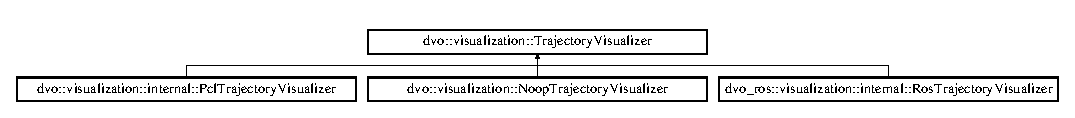
\includegraphics[height=1.131313cm]{classdvo_1_1visualization_1_1_trajectory_visualizer}
\end{center}
\end{figure}
\subsection*{Public Types}
\begin{DoxyCompactItemize}
\item 
typedef boost\+::shared\+\_\+ptr$<$ \mbox{\hyperlink{classdvo_1_1visualization_1_1_trajectory_visualizer}{Trajectory\+Visualizer}} $>$ \mbox{\hyperlink{classdvo_1_1visualization_1_1_trajectory_visualizer_aac33ef5979fe64ee33409f1afa977fd3}{Ptr}}
\end{DoxyCompactItemize}
\subsection*{Public Member Functions}
\begin{DoxyCompactItemize}
\item 
virtual \mbox{\hyperlink{classdvo_1_1visualization_1_1_trajectory_visualizer_ae0cd566f18de34fd8754ae3a419f84b9}{$\sim$\+Trajectory\+Visualizer}} ()
\item 
\mbox{\hyperlink{classdvo_1_1visualization_1_1_trajectory_visualizer_a037f387986028db6c8f9c18bc080b9c2}{F\+I\+\_\+\+A\+T\+T\+R\+I\+B\+U\+TE}} (\mbox{\hyperlink{classdvo_1_1visualization_1_1_trajectory_visualizer}{Trajectory\+Visualizer}}, std\+::string, name)
\item 
\mbox{\hyperlink{classdvo_1_1visualization_1_1_trajectory_visualizer_a023390bc025a00c0e08da2b91a7a2aec}{F\+I\+\_\+\+A\+T\+T\+R\+I\+B\+U\+TE}} (\mbox{\hyperlink{classdvo_1_1visualization_1_1_trajectory_visualizer}{Trajectory\+Visualizer}}, \mbox{\hyperlink{structdvo_1_1visualization_1_1_color}{Color}}, color)
\item 
virtual \mbox{\hyperlink{classdvo_1_1visualization_1_1_trajectory_visualizer}{Trajectory\+Visualizer}} \& \mbox{\hyperlink{classdvo_1_1visualization_1_1_trajectory_visualizer_ac41106ae7e28c019b03f0aa210c6f0c1}{add}} (const Eigen\+::\+Affine3d \&pose)=0
\end{DoxyCompactItemize}


\subsection{Member Typedef Documentation}
\mbox{\Hypertarget{classdvo_1_1visualization_1_1_trajectory_visualizer_aac33ef5979fe64ee33409f1afa977fd3}\label{classdvo_1_1visualization_1_1_trajectory_visualizer_aac33ef5979fe64ee33409f1afa977fd3}} 
\index{dvo\+::visualization\+::\+Trajectory\+Visualizer@{dvo\+::visualization\+::\+Trajectory\+Visualizer}!Ptr@{Ptr}}
\index{Ptr@{Ptr}!dvo\+::visualization\+::\+Trajectory\+Visualizer@{dvo\+::visualization\+::\+Trajectory\+Visualizer}}
\subsubsection{\texorpdfstring{Ptr}{Ptr}}
{\footnotesize\ttfamily typedef boost\+::shared\+\_\+ptr$<$\mbox{\hyperlink{classdvo_1_1visualization_1_1_trajectory_visualizer}{Trajectory\+Visualizer}}$>$ \mbox{\hyperlink{classdvo_1_1visualization_1_1_trajectory_visualizer_aac33ef5979fe64ee33409f1afa977fd3}{dvo\+::visualization\+::\+Trajectory\+Visualizer\+::\+Ptr}}}



\subsection{Constructor \& Destructor Documentation}
\mbox{\Hypertarget{classdvo_1_1visualization_1_1_trajectory_visualizer_ae0cd566f18de34fd8754ae3a419f84b9}\label{classdvo_1_1visualization_1_1_trajectory_visualizer_ae0cd566f18de34fd8754ae3a419f84b9}} 
\index{dvo\+::visualization\+::\+Trajectory\+Visualizer@{dvo\+::visualization\+::\+Trajectory\+Visualizer}!````~Trajectory\+Visualizer@{$\sim$\+Trajectory\+Visualizer}}
\index{````~Trajectory\+Visualizer@{$\sim$\+Trajectory\+Visualizer}!dvo\+::visualization\+::\+Trajectory\+Visualizer@{dvo\+::visualization\+::\+Trajectory\+Visualizer}}
\subsubsection{\texorpdfstring{$\sim$\+Trajectory\+Visualizer()}{~TrajectoryVisualizer()}}
{\footnotesize\ttfamily virtual dvo\+::visualization\+::\+Trajectory\+Visualizer\+::$\sim$\+Trajectory\+Visualizer (\begin{DoxyParamCaption}{ }\end{DoxyParamCaption})\hspace{0.3cm}{\ttfamily [inline]}, {\ttfamily [virtual]}}



\subsection{Member Function Documentation}
\mbox{\Hypertarget{classdvo_1_1visualization_1_1_trajectory_visualizer_ac41106ae7e28c019b03f0aa210c6f0c1}\label{classdvo_1_1visualization_1_1_trajectory_visualizer_ac41106ae7e28c019b03f0aa210c6f0c1}} 
\index{dvo\+::visualization\+::\+Trajectory\+Visualizer@{dvo\+::visualization\+::\+Trajectory\+Visualizer}!add@{add}}
\index{add@{add}!dvo\+::visualization\+::\+Trajectory\+Visualizer@{dvo\+::visualization\+::\+Trajectory\+Visualizer}}
\subsubsection{\texorpdfstring{add()}{add()}}
{\footnotesize\ttfamily virtual \mbox{\hyperlink{classdvo_1_1visualization_1_1_trajectory_visualizer}{Trajectory\+Visualizer}}\& dvo\+::visualization\+::\+Trajectory\+Visualizer\+::add (\begin{DoxyParamCaption}\item[{const Eigen\+::\+Affine3d \&}]{pose }\end{DoxyParamCaption})\hspace{0.3cm}{\ttfamily [pure virtual]}}



Implemented in \mbox{\hyperlink{classdvo__ros_1_1visualization_1_1internal_1_1_ros_trajectory_visualizer_acd66991b88e68e9843028cb5cb65c29a}{dvo\+\_\+ros\+::visualization\+::internal\+::\+Ros\+Trajectory\+Visualizer}}, \mbox{\hyperlink{classdvo_1_1visualization_1_1internal_1_1_pcl_trajectory_visualizer_aa174b5910657b2bfed45dfacd429a75a}{dvo\+::visualization\+::internal\+::\+Pcl\+Trajectory\+Visualizer}}, and \mbox{\hyperlink{classdvo_1_1visualization_1_1_noop_trajectory_visualizer_a40e9cfd01744c3efa85afb93237e2030}{dvo\+::visualization\+::\+Noop\+Trajectory\+Visualizer}}.

\mbox{\Hypertarget{classdvo_1_1visualization_1_1_trajectory_visualizer_a037f387986028db6c8f9c18bc080b9c2}\label{classdvo_1_1visualization_1_1_trajectory_visualizer_a037f387986028db6c8f9c18bc080b9c2}} 
\index{dvo\+::visualization\+::\+Trajectory\+Visualizer@{dvo\+::visualization\+::\+Trajectory\+Visualizer}!F\+I\+\_\+\+A\+T\+T\+R\+I\+B\+U\+TE@{F\+I\+\_\+\+A\+T\+T\+R\+I\+B\+U\+TE}}
\index{F\+I\+\_\+\+A\+T\+T\+R\+I\+B\+U\+TE@{F\+I\+\_\+\+A\+T\+T\+R\+I\+B\+U\+TE}!dvo\+::visualization\+::\+Trajectory\+Visualizer@{dvo\+::visualization\+::\+Trajectory\+Visualizer}}
\subsubsection{\texorpdfstring{F\+I\+\_\+\+A\+T\+T\+R\+I\+B\+U\+T\+E()}{FI\_ATTRIBUTE()}\hspace{0.1cm}{\footnotesize\ttfamily [1/2]}}
{\footnotesize\ttfamily dvo\+::visualization\+::\+Trajectory\+Visualizer\+::\+F\+I\+\_\+\+A\+T\+T\+R\+I\+B\+U\+TE (\begin{DoxyParamCaption}\item[{\mbox{\hyperlink{classdvo_1_1visualization_1_1_trajectory_visualizer}{Trajectory\+Visualizer}}}]{,  }\item[{std\+::string}]{,  }\item[{name}]{ }\end{DoxyParamCaption})}

\mbox{\Hypertarget{classdvo_1_1visualization_1_1_trajectory_visualizer_a023390bc025a00c0e08da2b91a7a2aec}\label{classdvo_1_1visualization_1_1_trajectory_visualizer_a023390bc025a00c0e08da2b91a7a2aec}} 
\index{dvo\+::visualization\+::\+Trajectory\+Visualizer@{dvo\+::visualization\+::\+Trajectory\+Visualizer}!F\+I\+\_\+\+A\+T\+T\+R\+I\+B\+U\+TE@{F\+I\+\_\+\+A\+T\+T\+R\+I\+B\+U\+TE}}
\index{F\+I\+\_\+\+A\+T\+T\+R\+I\+B\+U\+TE@{F\+I\+\_\+\+A\+T\+T\+R\+I\+B\+U\+TE}!dvo\+::visualization\+::\+Trajectory\+Visualizer@{dvo\+::visualization\+::\+Trajectory\+Visualizer}}
\subsubsection{\texorpdfstring{F\+I\+\_\+\+A\+T\+T\+R\+I\+B\+U\+T\+E()}{FI\_ATTRIBUTE()}\hspace{0.1cm}{\footnotesize\ttfamily [2/2]}}
{\footnotesize\ttfamily dvo\+::visualization\+::\+Trajectory\+Visualizer\+::\+F\+I\+\_\+\+A\+T\+T\+R\+I\+B\+U\+TE (\begin{DoxyParamCaption}\item[{\mbox{\hyperlink{classdvo_1_1visualization_1_1_trajectory_visualizer}{Trajectory\+Visualizer}}}]{,  }\item[{\mbox{\hyperlink{structdvo_1_1visualization_1_1_color}{Color}}}]{,  }\item[{color}]{ }\end{DoxyParamCaption})}



The documentation for this class was generated from the following file\+:\begin{DoxyCompactItemize}
\item 
dvo\+\_\+core/include/dvo/visualization/\mbox{\hyperlink{camera__trajectory__visualizer_8h}{camera\+\_\+trajectory\+\_\+visualizer.\+h}}\end{DoxyCompactItemize}

\hypertarget{classdvo_1_1core_1_1_tukey_influence_function}{}\section{dvo\+:\+:core\+:\+:Tukey\+Influence\+Function Class Reference}
\label{classdvo_1_1core_1_1_tukey_influence_function}\index{dvo\+::core\+::\+Tukey\+Influence\+Function@{dvo\+::core\+::\+Tukey\+Influence\+Function}}


{\ttfamily \#include $<$weight\+\_\+calculation.\+h$>$}

Inheritance diagram for dvo\+:\+:core\+:\+:Tukey\+Influence\+Function\+:\begin{figure}[H]
\begin{center}
\leavevmode
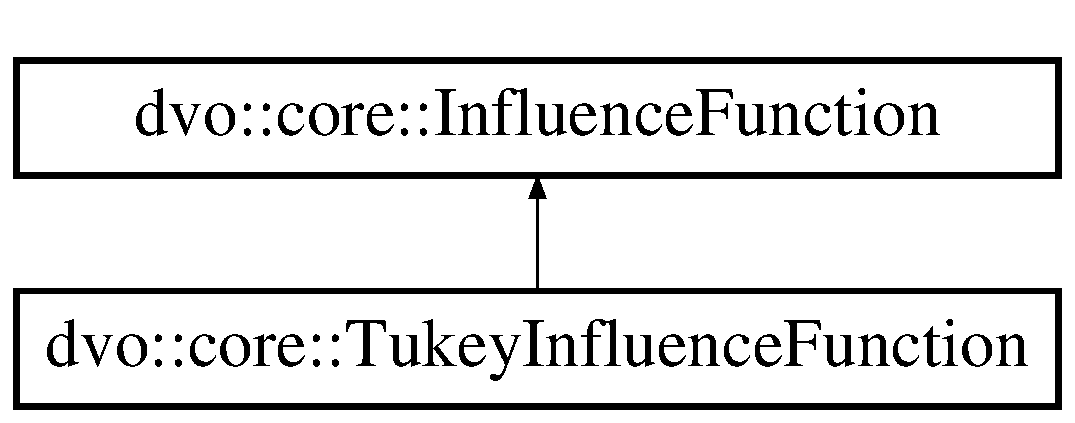
\includegraphics[height=2.000000cm]{classdvo_1_1core_1_1_tukey_influence_function}
\end{center}
\end{figure}
\subsection*{Public Member Functions}
\begin{DoxyCompactItemize}
\item 
\mbox{\hyperlink{classdvo_1_1core_1_1_tukey_influence_function_a5cce8b94396e7065d59fea7ef80fd768}{Tukey\+Influence\+Function}} (const float b=\mbox{\hyperlink{classdvo_1_1core_1_1_tukey_influence_function_a4abcd23e283b3152de20aaf8eb092e26}{D\+E\+F\+A\+U\+L\+T\+\_\+B}})
\item 
virtual \mbox{\hyperlink{classdvo_1_1core_1_1_tukey_influence_function_a754e8e9a16c391fa9234bc8c47183567}{$\sim$\+Tukey\+Influence\+Function}} ()
\item 
virtual float \mbox{\hyperlink{classdvo_1_1core_1_1_tukey_influence_function_a3a1829e6316ecffdceea8c54169c5ef1}{value}} (const float \&x) const
\item 
virtual void \mbox{\hyperlink{classdvo_1_1core_1_1_tukey_influence_function_afa49d538d3eee4c545bb690a0aca0f11}{configure}} (const float \&param)
\end{DoxyCompactItemize}
\subsection*{Static Public Attributes}
\begin{DoxyCompactItemize}
\item 
static const float \mbox{\hyperlink{classdvo_1_1core_1_1_tukey_influence_function_a4abcd23e283b3152de20aaf8eb092e26}{D\+E\+F\+A\+U\+L\+T\+\_\+B}} = 4.\+6851f
\end{DoxyCompactItemize}


\subsection{Detailed Description}
Tukey\textquotesingle{}s hard re-\/descending function.

See\+: \href{http://en.wikipedia.org/wiki/Redescending_M-estimator}{\tt http\+://en.\+wikipedia.\+org/wiki/\+Redescending\+\_\+\+M-\/estimator} 

\subsection{Constructor \& Destructor Documentation}
\mbox{\Hypertarget{classdvo_1_1core_1_1_tukey_influence_function_a5cce8b94396e7065d59fea7ef80fd768}\label{classdvo_1_1core_1_1_tukey_influence_function_a5cce8b94396e7065d59fea7ef80fd768}} 
\index{dvo\+::core\+::\+Tukey\+Influence\+Function@{dvo\+::core\+::\+Tukey\+Influence\+Function}!Tukey\+Influence\+Function@{Tukey\+Influence\+Function}}
\index{Tukey\+Influence\+Function@{Tukey\+Influence\+Function}!dvo\+::core\+::\+Tukey\+Influence\+Function@{dvo\+::core\+::\+Tukey\+Influence\+Function}}
\subsubsection{\texorpdfstring{Tukey\+Influence\+Function()}{TukeyInfluenceFunction()}}
{\footnotesize\ttfamily dvo\+::core\+::\+Tukey\+Influence\+Function\+::\+Tukey\+Influence\+Function (\begin{DoxyParamCaption}\item[{const float}]{b = {\ttfamily \mbox{\hyperlink{classdvo_1_1core_1_1_tukey_influence_function_a4abcd23e283b3152de20aaf8eb092e26}{D\+E\+F\+A\+U\+L\+T\+\_\+B}}} }\end{DoxyParamCaption})}

\mbox{\Hypertarget{classdvo_1_1core_1_1_tukey_influence_function_a754e8e9a16c391fa9234bc8c47183567}\label{classdvo_1_1core_1_1_tukey_influence_function_a754e8e9a16c391fa9234bc8c47183567}} 
\index{dvo\+::core\+::\+Tukey\+Influence\+Function@{dvo\+::core\+::\+Tukey\+Influence\+Function}!````~Tukey\+Influence\+Function@{$\sim$\+Tukey\+Influence\+Function}}
\index{````~Tukey\+Influence\+Function@{$\sim$\+Tukey\+Influence\+Function}!dvo\+::core\+::\+Tukey\+Influence\+Function@{dvo\+::core\+::\+Tukey\+Influence\+Function}}
\subsubsection{\texorpdfstring{$\sim$\+Tukey\+Influence\+Function()}{~TukeyInfluenceFunction()}}
{\footnotesize\ttfamily virtual dvo\+::core\+::\+Tukey\+Influence\+Function\+::$\sim$\+Tukey\+Influence\+Function (\begin{DoxyParamCaption}{ }\end{DoxyParamCaption})\hspace{0.3cm}{\ttfamily [inline]}, {\ttfamily [virtual]}}



\subsection{Member Function Documentation}
\mbox{\Hypertarget{classdvo_1_1core_1_1_tukey_influence_function_afa49d538d3eee4c545bb690a0aca0f11}\label{classdvo_1_1core_1_1_tukey_influence_function_afa49d538d3eee4c545bb690a0aca0f11}} 
\index{dvo\+::core\+::\+Tukey\+Influence\+Function@{dvo\+::core\+::\+Tukey\+Influence\+Function}!configure@{configure}}
\index{configure@{configure}!dvo\+::core\+::\+Tukey\+Influence\+Function@{dvo\+::core\+::\+Tukey\+Influence\+Function}}
\subsubsection{\texorpdfstring{configure()}{configure()}}
{\footnotesize\ttfamily void dvo\+::core\+::\+Tukey\+Influence\+Function\+::configure (\begin{DoxyParamCaption}\item[{const float \&}]{param }\end{DoxyParamCaption})\hspace{0.3cm}{\ttfamily [virtual]}}



Reimplemented from \mbox{\hyperlink{classdvo_1_1core_1_1_influence_function_a4773b03ca609bc5d8391d09d92ab34ad}{dvo\+::core\+::\+Influence\+Function}}.

\mbox{\Hypertarget{classdvo_1_1core_1_1_tukey_influence_function_a3a1829e6316ecffdceea8c54169c5ef1}\label{classdvo_1_1core_1_1_tukey_influence_function_a3a1829e6316ecffdceea8c54169c5ef1}} 
\index{dvo\+::core\+::\+Tukey\+Influence\+Function@{dvo\+::core\+::\+Tukey\+Influence\+Function}!value@{value}}
\index{value@{value}!dvo\+::core\+::\+Tukey\+Influence\+Function@{dvo\+::core\+::\+Tukey\+Influence\+Function}}
\subsubsection{\texorpdfstring{value()}{value()}}
{\footnotesize\ttfamily float dvo\+::core\+::\+Tukey\+Influence\+Function\+::value (\begin{DoxyParamCaption}\item[{const float \&}]{x }\end{DoxyParamCaption}) const\hspace{0.3cm}{\ttfamily [inline]}, {\ttfamily [virtual]}}



Implements \mbox{\hyperlink{classdvo_1_1core_1_1_influence_function_a158082c763fa9de460e75a285bb91f1e}{dvo\+::core\+::\+Influence\+Function}}.



\subsection{Member Data Documentation}
\mbox{\Hypertarget{classdvo_1_1core_1_1_tukey_influence_function_a4abcd23e283b3152de20aaf8eb092e26}\label{classdvo_1_1core_1_1_tukey_influence_function_a4abcd23e283b3152de20aaf8eb092e26}} 
\index{dvo\+::core\+::\+Tukey\+Influence\+Function@{dvo\+::core\+::\+Tukey\+Influence\+Function}!D\+E\+F\+A\+U\+L\+T\+\_\+B@{D\+E\+F\+A\+U\+L\+T\+\_\+B}}
\index{D\+E\+F\+A\+U\+L\+T\+\_\+B@{D\+E\+F\+A\+U\+L\+T\+\_\+B}!dvo\+::core\+::\+Tukey\+Influence\+Function@{dvo\+::core\+::\+Tukey\+Influence\+Function}}
\subsubsection{\texorpdfstring{D\+E\+F\+A\+U\+L\+T\+\_\+B}{DEFAULT\_B}}
{\footnotesize\ttfamily const float dvo\+::core\+::\+Tukey\+Influence\+Function\+::\+D\+E\+F\+A\+U\+L\+T\+\_\+B = 4.\+6851f\hspace{0.3cm}{\ttfamily [static]}}



The documentation for this class was generated from the following files\+:\begin{DoxyCompactItemize}
\item 
dvo\+\_\+core/include/dvo/core/\mbox{\hyperlink{weight__calculation_8h}{weight\+\_\+calculation.\+h}}\item 
dvo\+\_\+core/src/core/\mbox{\hyperlink{weight__calculation_8cpp}{weight\+\_\+calculation.\+cpp}}\end{DoxyCompactItemize}

\hypertarget{classdvo_1_1core_1_1_unit_influence_function}{}\section{dvo\+:\+:core\+:\+:Unit\+Influence\+Function Class Reference}
\label{classdvo_1_1core_1_1_unit_influence_function}\index{dvo\+::core\+::\+Unit\+Influence\+Function@{dvo\+::core\+::\+Unit\+Influence\+Function}}


{\ttfamily \#include $<$weight\+\_\+calculation.\+h$>$}

Inheritance diagram for dvo\+:\+:core\+:\+:Unit\+Influence\+Function\+:\begin{figure}[H]
\begin{center}
\leavevmode
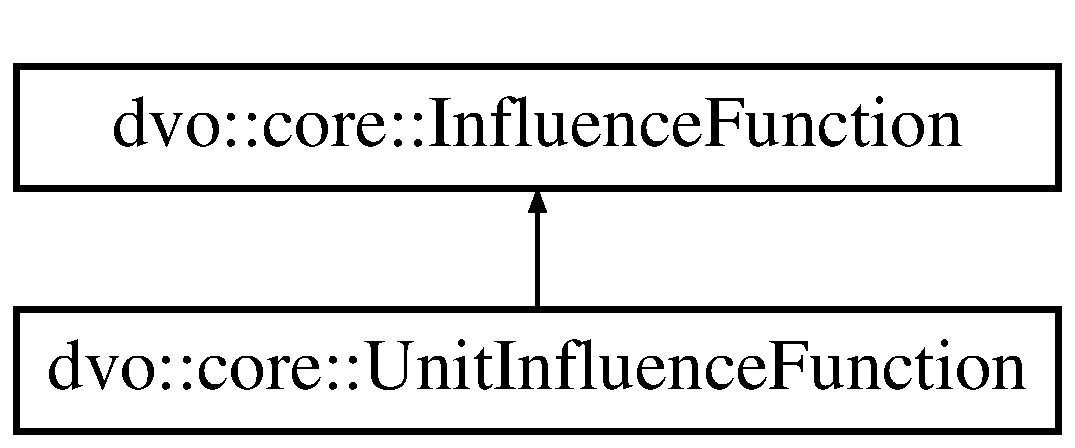
\includegraphics[height=2.000000cm]{classdvo_1_1core_1_1_unit_influence_function}
\end{center}
\end{figure}
\subsection*{Public Member Functions}
\begin{DoxyCompactItemize}
\item 
\mbox{\hyperlink{classdvo_1_1core_1_1_unit_influence_function_ae311eee27c2c13cb271c8c16abaf84fb}{Unit\+Influence\+Function}} ()
\item 
virtual \mbox{\hyperlink{classdvo_1_1core_1_1_unit_influence_function_a1d72e24e73a9b8ca22edadded2dcfe3b}{$\sim$\+Unit\+Influence\+Function}} ()
\item 
virtual float \mbox{\hyperlink{classdvo_1_1core_1_1_unit_influence_function_a889eacebc6bcb0209a8ce37742dbbe71}{value}} (const float \&x) const
\end{DoxyCompactItemize}


\subsection{Constructor \& Destructor Documentation}
\mbox{\Hypertarget{classdvo_1_1core_1_1_unit_influence_function_ae311eee27c2c13cb271c8c16abaf84fb}\label{classdvo_1_1core_1_1_unit_influence_function_ae311eee27c2c13cb271c8c16abaf84fb}} 
\index{dvo\+::core\+::\+Unit\+Influence\+Function@{dvo\+::core\+::\+Unit\+Influence\+Function}!Unit\+Influence\+Function@{Unit\+Influence\+Function}}
\index{Unit\+Influence\+Function@{Unit\+Influence\+Function}!dvo\+::core\+::\+Unit\+Influence\+Function@{dvo\+::core\+::\+Unit\+Influence\+Function}}
\subsubsection{\texorpdfstring{Unit\+Influence\+Function()}{UnitInfluenceFunction()}}
{\footnotesize\ttfamily dvo\+::core\+::\+Unit\+Influence\+Function\+::\+Unit\+Influence\+Function (\begin{DoxyParamCaption}{ }\end{DoxyParamCaption})\hspace{0.3cm}{\ttfamily [inline]}}

\mbox{\Hypertarget{classdvo_1_1core_1_1_unit_influence_function_a1d72e24e73a9b8ca22edadded2dcfe3b}\label{classdvo_1_1core_1_1_unit_influence_function_a1d72e24e73a9b8ca22edadded2dcfe3b}} 
\index{dvo\+::core\+::\+Unit\+Influence\+Function@{dvo\+::core\+::\+Unit\+Influence\+Function}!````~Unit\+Influence\+Function@{$\sim$\+Unit\+Influence\+Function}}
\index{````~Unit\+Influence\+Function@{$\sim$\+Unit\+Influence\+Function}!dvo\+::core\+::\+Unit\+Influence\+Function@{dvo\+::core\+::\+Unit\+Influence\+Function}}
\subsubsection{\texorpdfstring{$\sim$\+Unit\+Influence\+Function()}{~UnitInfluenceFunction()}}
{\footnotesize\ttfamily virtual dvo\+::core\+::\+Unit\+Influence\+Function\+::$\sim$\+Unit\+Influence\+Function (\begin{DoxyParamCaption}{ }\end{DoxyParamCaption})\hspace{0.3cm}{\ttfamily [inline]}, {\ttfamily [virtual]}}



\subsection{Member Function Documentation}
\mbox{\Hypertarget{classdvo_1_1core_1_1_unit_influence_function_a889eacebc6bcb0209a8ce37742dbbe71}\label{classdvo_1_1core_1_1_unit_influence_function_a889eacebc6bcb0209a8ce37742dbbe71}} 
\index{dvo\+::core\+::\+Unit\+Influence\+Function@{dvo\+::core\+::\+Unit\+Influence\+Function}!value@{value}}
\index{value@{value}!dvo\+::core\+::\+Unit\+Influence\+Function@{dvo\+::core\+::\+Unit\+Influence\+Function}}
\subsubsection{\texorpdfstring{value()}{value()}}
{\footnotesize\ttfamily virtual float dvo\+::core\+::\+Unit\+Influence\+Function\+::value (\begin{DoxyParamCaption}\item[{const float \&}]{x }\end{DoxyParamCaption}) const\hspace{0.3cm}{\ttfamily [inline]}, {\ttfamily [virtual]}}



Implements \mbox{\hyperlink{classdvo_1_1core_1_1_influence_function_a158082c763fa9de460e75a285bb91f1e}{dvo\+::core\+::\+Influence\+Function}}.



The documentation for this class was generated from the following file\+:\begin{DoxyCompactItemize}
\item 
dvo\+\_\+core/include/dvo/core/\mbox{\hyperlink{weight__calculation_8h}{weight\+\_\+calculation.\+h}}\end{DoxyCompactItemize}

\hypertarget{classdvo_1_1core_1_1_unit_scale_estimator}{}\section{dvo\+:\+:core\+:\+:Unit\+Scale\+Estimator Class Reference}
\label{classdvo_1_1core_1_1_unit_scale_estimator}\index{dvo\+::core\+::\+Unit\+Scale\+Estimator@{dvo\+::core\+::\+Unit\+Scale\+Estimator}}


{\ttfamily \#include $<$weight\+\_\+calculation.\+h$>$}

Inheritance diagram for dvo\+:\+:core\+:\+:Unit\+Scale\+Estimator\+:\begin{figure}[H]
\begin{center}
\leavevmode
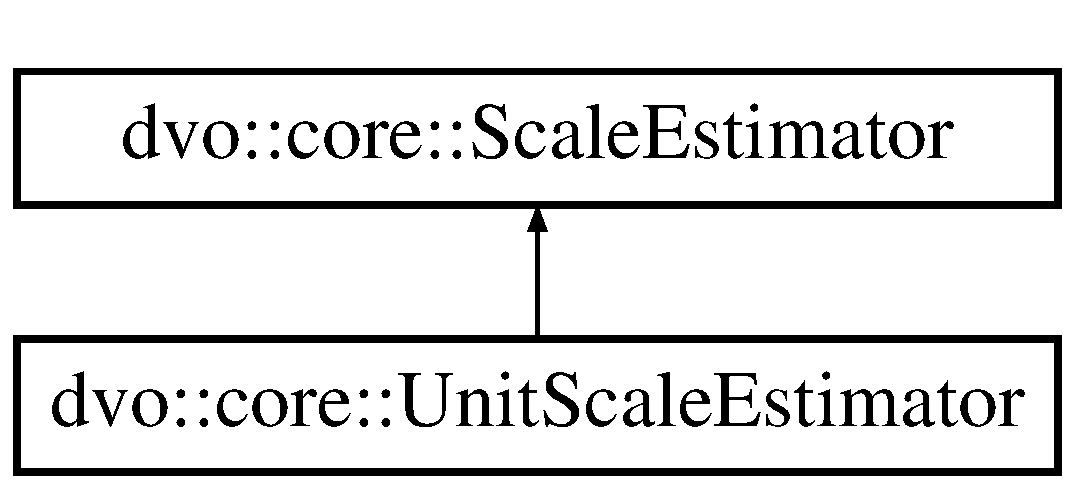
\includegraphics[height=2.000000cm]{classdvo_1_1core_1_1_unit_scale_estimator}
\end{center}
\end{figure}
\subsection*{Public Member Functions}
\begin{DoxyCompactItemize}
\item 
\mbox{\hyperlink{classdvo_1_1core_1_1_unit_scale_estimator_a848f562d555626a06004987f03f0bc32}{Unit\+Scale\+Estimator}} ()
\item 
virtual \mbox{\hyperlink{classdvo_1_1core_1_1_unit_scale_estimator_ab3314993ec55499d0693ce7310e13de9}{$\sim$\+Unit\+Scale\+Estimator}} ()
\item 
virtual float \mbox{\hyperlink{classdvo_1_1core_1_1_unit_scale_estimator_a7578f9008f25d96250c20ff3080673ed}{compute}} (const cv\+::\+Mat \&errors) const
\end{DoxyCompactItemize}


\subsection{Constructor \& Destructor Documentation}
\mbox{\Hypertarget{classdvo_1_1core_1_1_unit_scale_estimator_a848f562d555626a06004987f03f0bc32}\label{classdvo_1_1core_1_1_unit_scale_estimator_a848f562d555626a06004987f03f0bc32}} 
\index{dvo\+::core\+::\+Unit\+Scale\+Estimator@{dvo\+::core\+::\+Unit\+Scale\+Estimator}!Unit\+Scale\+Estimator@{Unit\+Scale\+Estimator}}
\index{Unit\+Scale\+Estimator@{Unit\+Scale\+Estimator}!dvo\+::core\+::\+Unit\+Scale\+Estimator@{dvo\+::core\+::\+Unit\+Scale\+Estimator}}
\subsubsection{\texorpdfstring{Unit\+Scale\+Estimator()}{UnitScaleEstimator()}}
{\footnotesize\ttfamily dvo\+::core\+::\+Unit\+Scale\+Estimator\+::\+Unit\+Scale\+Estimator (\begin{DoxyParamCaption}{ }\end{DoxyParamCaption})\hspace{0.3cm}{\ttfamily [inline]}}

\mbox{\Hypertarget{classdvo_1_1core_1_1_unit_scale_estimator_ab3314993ec55499d0693ce7310e13de9}\label{classdvo_1_1core_1_1_unit_scale_estimator_ab3314993ec55499d0693ce7310e13de9}} 
\index{dvo\+::core\+::\+Unit\+Scale\+Estimator@{dvo\+::core\+::\+Unit\+Scale\+Estimator}!````~Unit\+Scale\+Estimator@{$\sim$\+Unit\+Scale\+Estimator}}
\index{````~Unit\+Scale\+Estimator@{$\sim$\+Unit\+Scale\+Estimator}!dvo\+::core\+::\+Unit\+Scale\+Estimator@{dvo\+::core\+::\+Unit\+Scale\+Estimator}}
\subsubsection{\texorpdfstring{$\sim$\+Unit\+Scale\+Estimator()}{~UnitScaleEstimator()}}
{\footnotesize\ttfamily virtual dvo\+::core\+::\+Unit\+Scale\+Estimator\+::$\sim$\+Unit\+Scale\+Estimator (\begin{DoxyParamCaption}{ }\end{DoxyParamCaption})\hspace{0.3cm}{\ttfamily [inline]}, {\ttfamily [virtual]}}



\subsection{Member Function Documentation}
\mbox{\Hypertarget{classdvo_1_1core_1_1_unit_scale_estimator_a7578f9008f25d96250c20ff3080673ed}\label{classdvo_1_1core_1_1_unit_scale_estimator_a7578f9008f25d96250c20ff3080673ed}} 
\index{dvo\+::core\+::\+Unit\+Scale\+Estimator@{dvo\+::core\+::\+Unit\+Scale\+Estimator}!compute@{compute}}
\index{compute@{compute}!dvo\+::core\+::\+Unit\+Scale\+Estimator@{dvo\+::core\+::\+Unit\+Scale\+Estimator}}
\subsubsection{\texorpdfstring{compute()}{compute()}}
{\footnotesize\ttfamily virtual float dvo\+::core\+::\+Unit\+Scale\+Estimator\+::compute (\begin{DoxyParamCaption}\item[{const cv\+::\+Mat \&}]{errors }\end{DoxyParamCaption}) const\hspace{0.3cm}{\ttfamily [inline]}, {\ttfamily [virtual]}}



Implements \mbox{\hyperlink{classdvo_1_1core_1_1_scale_estimator_a6968ac2cd37c2ce1c966f0c9e17d1a3c}{dvo\+::core\+::\+Scale\+Estimator}}.



The documentation for this class was generated from the following file\+:\begin{DoxyCompactItemize}
\item 
dvo\+\_\+core/include/dvo/core/\mbox{\hyperlink{weight__calculation_8h}{weight\+\_\+calculation.\+h}}\end{DoxyCompactItemize}

\hypertarget{classdvo_1_1visualization_1_1_visualizer}{}\section{dvo\+:\+:visualization\+:\+:Visualizer Class Reference}
\label{classdvo_1_1visualization_1_1_visualizer}\index{dvo\+::visualization\+::\+Visualizer@{dvo\+::visualization\+::\+Visualizer}}


{\ttfamily \#include $<$visualizer.\+h$>$}

\subsection*{Public Types}
\begin{DoxyCompactItemize}
\item 
typedef boost\+::function$<$ void(cv\+::\+Mat \&)$>$ \mbox{\hyperlink{classdvo_1_1visualization_1_1_visualizer_ac33e0b53e7ef7be64e3230f6c91084a0}{Image\+Modifier}}
\end{DoxyCompactItemize}
\subsection*{Public Member Functions}
\begin{DoxyCompactItemize}
\item 
\mbox{\hyperlink{classdvo_1_1visualization_1_1_visualizer}{Visualizer}} \& \mbox{\hyperlink{classdvo_1_1visualization_1_1_visualizer_add2fa4993814327d9153aafcda1fea6f}{show}} (const char $\ast$name, const cv\+::\+Mat\+Expr \&img, \mbox{\hyperlink{classdvo_1_1visualization_1_1_visualizer_ac33e0b53e7ef7be64e3230f6c91084a0}{Image\+Modifier}} modifier=\mbox{\hyperlink{classdvo_1_1visualization_1_1_visualizer_ac33e0b53e7ef7be64e3230f6c91084a0}{Image\+Modifier}}())
\item 
\mbox{\hyperlink{classdvo_1_1visualization_1_1_visualizer}{Visualizer}} \& \mbox{\hyperlink{classdvo_1_1visualization_1_1_visualizer_a1dea5a2108f022dfc92ec0eb0aa3a717}{show}} (std\+::string \&name, const cv\+::\+Mat\+Expr \&img, \mbox{\hyperlink{classdvo_1_1visualization_1_1_visualizer_ac33e0b53e7ef7be64e3230f6c91084a0}{Image\+Modifier}} modifier=\mbox{\hyperlink{classdvo_1_1visualization_1_1_visualizer_ac33e0b53e7ef7be64e3230f6c91084a0}{Image\+Modifier}}())
\item 
\mbox{\hyperlink{classdvo_1_1visualization_1_1_visualizer}{Visualizer}} \& \mbox{\hyperlink{classdvo_1_1visualization_1_1_visualizer_a4bf94bdc655c4723e71559de479eae44}{show}} (const char $\ast$name, const cv\+::\+Mat \&img, \mbox{\hyperlink{classdvo_1_1visualization_1_1_visualizer_ac33e0b53e7ef7be64e3230f6c91084a0}{Image\+Modifier}} modifier=\mbox{\hyperlink{classdvo_1_1visualization_1_1_visualizer_ac33e0b53e7ef7be64e3230f6c91084a0}{Image\+Modifier}}())
\item 
\mbox{\hyperlink{classdvo_1_1visualization_1_1_visualizer}{Visualizer}} \& \mbox{\hyperlink{classdvo_1_1visualization_1_1_visualizer_a5d7ddfc5ada5e75da5d9ddb428e17d24}{show}} (std\+::string \&name, const cv\+::\+Mat \&img, \mbox{\hyperlink{classdvo_1_1visualization_1_1_visualizer_ac33e0b53e7ef7be64e3230f6c91084a0}{Image\+Modifier}} modifier=\mbox{\hyperlink{classdvo_1_1visualization_1_1_visualizer_ac33e0b53e7ef7be64e3230f6c91084a0}{Image\+Modifier}}())
\item 
\mbox{\hyperlink{classdvo_1_1visualization_1_1_visualizer}{Visualizer}} \& \mbox{\hyperlink{classdvo_1_1visualization_1_1_visualizer_a11a1116999ef58353e695a62339bb1c4}{show\+Histogram}} (const char $\ast$name, const cv\+::\+Mat \&img, float binsize, float min, float max)
\item 
\mbox{\hyperlink{classdvo_1_1visualization_1_1_visualizer}{Visualizer}} \& \mbox{\hyperlink{classdvo_1_1visualization_1_1_visualizer_aca408d9ab7e8e8fc8f9f7c3dd40f0457}{show\+Histogram}} (std\+::string \&name, const cv\+::\+Mat \&img, float binsize, float min, float max)
\item 
\mbox{\hyperlink{classdvo_1_1visualization_1_1_visualizer}{Visualizer}} \& \mbox{\hyperlink{classdvo_1_1visualization_1_1_visualizer_adc47051ac9cbd39cbc94992511137bd6}{use\+External\+Wait\+Key}} (bool value)
\item 
bool \mbox{\hyperlink{classdvo_1_1visualization_1_1_visualizer_a19a81ff0cc68145986c13b1da09affb0}{use\+External\+Wait\+Key}} () const
\item 
\mbox{\hyperlink{classdvo_1_1visualization_1_1_visualizer}{Visualizer}} \& \mbox{\hyperlink{classdvo_1_1visualization_1_1_visualizer_a514dfc248d0676c84161f38132c06cb8}{save}} (bool value)
\item 
bool \mbox{\hyperlink{classdvo_1_1visualization_1_1_visualizer_ad53a6d58f48de5063ca7c196005db380}{save}} () const
\end{DoxyCompactItemize}
\subsection*{Static Public Member Functions}
\begin{DoxyCompactItemize}
\item 
static \mbox{\hyperlink{classdvo_1_1visualization_1_1_visualizer}{Visualizer}} \& \mbox{\hyperlink{classdvo_1_1visualization_1_1_visualizer_a97dc12917863ab3379cea320844c798b}{instance}} ()
\end{DoxyCompactItemize}


\subsection{Member Typedef Documentation}
\mbox{\Hypertarget{classdvo_1_1visualization_1_1_visualizer_ac33e0b53e7ef7be64e3230f6c91084a0}\label{classdvo_1_1visualization_1_1_visualizer_ac33e0b53e7ef7be64e3230f6c91084a0}} 
\index{dvo\+::visualization\+::\+Visualizer@{dvo\+::visualization\+::\+Visualizer}!Image\+Modifier@{Image\+Modifier}}
\index{Image\+Modifier@{Image\+Modifier}!dvo\+::visualization\+::\+Visualizer@{dvo\+::visualization\+::\+Visualizer}}
\subsubsection{\texorpdfstring{Image\+Modifier}{ImageModifier}}
{\footnotesize\ttfamily typedef boost\+::function$<$void(cv\+::\+Mat\&)$>$ \mbox{\hyperlink{classdvo_1_1visualization_1_1_visualizer_ac33e0b53e7ef7be64e3230f6c91084a0}{dvo\+::visualization\+::\+Visualizer\+::\+Image\+Modifier}}}



\subsection{Member Function Documentation}
\mbox{\Hypertarget{classdvo_1_1visualization_1_1_visualizer_a97dc12917863ab3379cea320844c798b}\label{classdvo_1_1visualization_1_1_visualizer_a97dc12917863ab3379cea320844c798b}} 
\index{dvo\+::visualization\+::\+Visualizer@{dvo\+::visualization\+::\+Visualizer}!instance@{instance}}
\index{instance@{instance}!dvo\+::visualization\+::\+Visualizer@{dvo\+::visualization\+::\+Visualizer}}
\subsubsection{\texorpdfstring{instance()}{instance()}}
{\footnotesize\ttfamily \mbox{\hyperlink{classdvo_1_1visualization_1_1_visualizer}{Visualizer}} \& dvo\+::visualization\+::\+Visualizer\+::instance (\begin{DoxyParamCaption}{ }\end{DoxyParamCaption})\hspace{0.3cm}{\ttfamily [static]}}

\mbox{\Hypertarget{classdvo_1_1visualization_1_1_visualizer_a514dfc248d0676c84161f38132c06cb8}\label{classdvo_1_1visualization_1_1_visualizer_a514dfc248d0676c84161f38132c06cb8}} 
\index{dvo\+::visualization\+::\+Visualizer@{dvo\+::visualization\+::\+Visualizer}!save@{save}}
\index{save@{save}!dvo\+::visualization\+::\+Visualizer@{dvo\+::visualization\+::\+Visualizer}}
\subsubsection{\texorpdfstring{save()}{save()}\hspace{0.1cm}{\footnotesize\ttfamily [1/2]}}
{\footnotesize\ttfamily \mbox{\hyperlink{classdvo_1_1visualization_1_1_visualizer}{Visualizer}} \& dvo\+::visualization\+::\+Visualizer\+::save (\begin{DoxyParamCaption}\item[{bool}]{value }\end{DoxyParamCaption})}

\mbox{\Hypertarget{classdvo_1_1visualization_1_1_visualizer_ad53a6d58f48de5063ca7c196005db380}\label{classdvo_1_1visualization_1_1_visualizer_ad53a6d58f48de5063ca7c196005db380}} 
\index{dvo\+::visualization\+::\+Visualizer@{dvo\+::visualization\+::\+Visualizer}!save@{save}}
\index{save@{save}!dvo\+::visualization\+::\+Visualizer@{dvo\+::visualization\+::\+Visualizer}}
\subsubsection{\texorpdfstring{save()}{save()}\hspace{0.1cm}{\footnotesize\ttfamily [2/2]}}
{\footnotesize\ttfamily bool dvo\+::visualization\+::\+Visualizer\+::save (\begin{DoxyParamCaption}{ }\end{DoxyParamCaption}) const}

\mbox{\Hypertarget{classdvo_1_1visualization_1_1_visualizer_add2fa4993814327d9153aafcda1fea6f}\label{classdvo_1_1visualization_1_1_visualizer_add2fa4993814327d9153aafcda1fea6f}} 
\index{dvo\+::visualization\+::\+Visualizer@{dvo\+::visualization\+::\+Visualizer}!show@{show}}
\index{show@{show}!dvo\+::visualization\+::\+Visualizer@{dvo\+::visualization\+::\+Visualizer}}
\subsubsection{\texorpdfstring{show()}{show()}\hspace{0.1cm}{\footnotesize\ttfamily [1/4]}}
{\footnotesize\ttfamily \mbox{\hyperlink{classdvo_1_1visualization_1_1_visualizer}{Visualizer}} \& dvo\+::visualization\+::\+Visualizer\+::show (\begin{DoxyParamCaption}\item[{const char $\ast$}]{name,  }\item[{const cv\+::\+Mat\+Expr \&}]{img,  }\item[{\mbox{\hyperlink{classdvo_1_1visualization_1_1_visualizer_ac33e0b53e7ef7be64e3230f6c91084a0}{Image\+Modifier}}}]{modifier = {\ttfamily \mbox{\hyperlink{classdvo_1_1visualization_1_1_visualizer_ac33e0b53e7ef7be64e3230f6c91084a0}{Image\+Modifier}}()} }\end{DoxyParamCaption})}

\mbox{\Hypertarget{classdvo_1_1visualization_1_1_visualizer_a1dea5a2108f022dfc92ec0eb0aa3a717}\label{classdvo_1_1visualization_1_1_visualizer_a1dea5a2108f022dfc92ec0eb0aa3a717}} 
\index{dvo\+::visualization\+::\+Visualizer@{dvo\+::visualization\+::\+Visualizer}!show@{show}}
\index{show@{show}!dvo\+::visualization\+::\+Visualizer@{dvo\+::visualization\+::\+Visualizer}}
\subsubsection{\texorpdfstring{show()}{show()}\hspace{0.1cm}{\footnotesize\ttfamily [2/4]}}
{\footnotesize\ttfamily \mbox{\hyperlink{classdvo_1_1visualization_1_1_visualizer}{Visualizer}} \& dvo\+::visualization\+::\+Visualizer\+::show (\begin{DoxyParamCaption}\item[{std\+::string \&}]{name,  }\item[{const cv\+::\+Mat\+Expr \&}]{img,  }\item[{\mbox{\hyperlink{classdvo_1_1visualization_1_1_visualizer_ac33e0b53e7ef7be64e3230f6c91084a0}{Image\+Modifier}}}]{modifier = {\ttfamily \mbox{\hyperlink{classdvo_1_1visualization_1_1_visualizer_ac33e0b53e7ef7be64e3230f6c91084a0}{Image\+Modifier}}()} }\end{DoxyParamCaption})}

\mbox{\Hypertarget{classdvo_1_1visualization_1_1_visualizer_a4bf94bdc655c4723e71559de479eae44}\label{classdvo_1_1visualization_1_1_visualizer_a4bf94bdc655c4723e71559de479eae44}} 
\index{dvo\+::visualization\+::\+Visualizer@{dvo\+::visualization\+::\+Visualizer}!show@{show}}
\index{show@{show}!dvo\+::visualization\+::\+Visualizer@{dvo\+::visualization\+::\+Visualizer}}
\subsubsection{\texorpdfstring{show()}{show()}\hspace{0.1cm}{\footnotesize\ttfamily [3/4]}}
{\footnotesize\ttfamily \mbox{\hyperlink{classdvo_1_1visualization_1_1_visualizer}{Visualizer}} \& dvo\+::visualization\+::\+Visualizer\+::show (\begin{DoxyParamCaption}\item[{const char $\ast$}]{name,  }\item[{const cv\+::\+Mat \&}]{img,  }\item[{\mbox{\hyperlink{classdvo_1_1visualization_1_1_visualizer_ac33e0b53e7ef7be64e3230f6c91084a0}{Image\+Modifier}}}]{modifier = {\ttfamily \mbox{\hyperlink{classdvo_1_1visualization_1_1_visualizer_ac33e0b53e7ef7be64e3230f6c91084a0}{Image\+Modifier}}()} }\end{DoxyParamCaption})}

\mbox{\Hypertarget{classdvo_1_1visualization_1_1_visualizer_a5d7ddfc5ada5e75da5d9ddb428e17d24}\label{classdvo_1_1visualization_1_1_visualizer_a5d7ddfc5ada5e75da5d9ddb428e17d24}} 
\index{dvo\+::visualization\+::\+Visualizer@{dvo\+::visualization\+::\+Visualizer}!show@{show}}
\index{show@{show}!dvo\+::visualization\+::\+Visualizer@{dvo\+::visualization\+::\+Visualizer}}
\subsubsection{\texorpdfstring{show()}{show()}\hspace{0.1cm}{\footnotesize\ttfamily [4/4]}}
{\footnotesize\ttfamily \mbox{\hyperlink{classdvo_1_1visualization_1_1_visualizer}{Visualizer}} \& dvo\+::visualization\+::\+Visualizer\+::show (\begin{DoxyParamCaption}\item[{std\+::string \&}]{name,  }\item[{const cv\+::\+Mat \&}]{img,  }\item[{\mbox{\hyperlink{classdvo_1_1visualization_1_1_visualizer_ac33e0b53e7ef7be64e3230f6c91084a0}{Image\+Modifier}}}]{modifier = {\ttfamily \mbox{\hyperlink{classdvo_1_1visualization_1_1_visualizer_ac33e0b53e7ef7be64e3230f6c91084a0}{Image\+Modifier}}()} }\end{DoxyParamCaption})}

\mbox{\Hypertarget{classdvo_1_1visualization_1_1_visualizer_a11a1116999ef58353e695a62339bb1c4}\label{classdvo_1_1visualization_1_1_visualizer_a11a1116999ef58353e695a62339bb1c4}} 
\index{dvo\+::visualization\+::\+Visualizer@{dvo\+::visualization\+::\+Visualizer}!show\+Histogram@{show\+Histogram}}
\index{show\+Histogram@{show\+Histogram}!dvo\+::visualization\+::\+Visualizer@{dvo\+::visualization\+::\+Visualizer}}
\subsubsection{\texorpdfstring{show\+Histogram()}{showHistogram()}\hspace{0.1cm}{\footnotesize\ttfamily [1/2]}}
{\footnotesize\ttfamily \mbox{\hyperlink{classdvo_1_1visualization_1_1_visualizer}{Visualizer}} \& dvo\+::visualization\+::\+Visualizer\+::show\+Histogram (\begin{DoxyParamCaption}\item[{const char $\ast$}]{name,  }\item[{const cv\+::\+Mat \&}]{img,  }\item[{float}]{binsize,  }\item[{float}]{min,  }\item[{float}]{max }\end{DoxyParamCaption})}

\mbox{\Hypertarget{classdvo_1_1visualization_1_1_visualizer_aca408d9ab7e8e8fc8f9f7c3dd40f0457}\label{classdvo_1_1visualization_1_1_visualizer_aca408d9ab7e8e8fc8f9f7c3dd40f0457}} 
\index{dvo\+::visualization\+::\+Visualizer@{dvo\+::visualization\+::\+Visualizer}!show\+Histogram@{show\+Histogram}}
\index{show\+Histogram@{show\+Histogram}!dvo\+::visualization\+::\+Visualizer@{dvo\+::visualization\+::\+Visualizer}}
\subsubsection{\texorpdfstring{show\+Histogram()}{showHistogram()}\hspace{0.1cm}{\footnotesize\ttfamily [2/2]}}
{\footnotesize\ttfamily \mbox{\hyperlink{classdvo_1_1visualization_1_1_visualizer}{Visualizer}} \& dvo\+::visualization\+::\+Visualizer\+::show\+Histogram (\begin{DoxyParamCaption}\item[{std\+::string \&}]{name,  }\item[{const cv\+::\+Mat \&}]{img,  }\item[{float}]{binsize,  }\item[{float}]{min,  }\item[{float}]{max }\end{DoxyParamCaption})}

\mbox{\Hypertarget{classdvo_1_1visualization_1_1_visualizer_adc47051ac9cbd39cbc94992511137bd6}\label{classdvo_1_1visualization_1_1_visualizer_adc47051ac9cbd39cbc94992511137bd6}} 
\index{dvo\+::visualization\+::\+Visualizer@{dvo\+::visualization\+::\+Visualizer}!use\+External\+Wait\+Key@{use\+External\+Wait\+Key}}
\index{use\+External\+Wait\+Key@{use\+External\+Wait\+Key}!dvo\+::visualization\+::\+Visualizer@{dvo\+::visualization\+::\+Visualizer}}
\subsubsection{\texorpdfstring{use\+External\+Wait\+Key()}{useExternalWaitKey()}\hspace{0.1cm}{\footnotesize\ttfamily [1/2]}}
{\footnotesize\ttfamily \mbox{\hyperlink{classdvo_1_1visualization_1_1_visualizer}{Visualizer}} \& dvo\+::visualization\+::\+Visualizer\+::use\+External\+Wait\+Key (\begin{DoxyParamCaption}\item[{bool}]{value }\end{DoxyParamCaption})}

\mbox{\Hypertarget{classdvo_1_1visualization_1_1_visualizer_a19a81ff0cc68145986c13b1da09affb0}\label{classdvo_1_1visualization_1_1_visualizer_a19a81ff0cc68145986c13b1da09affb0}} 
\index{dvo\+::visualization\+::\+Visualizer@{dvo\+::visualization\+::\+Visualizer}!use\+External\+Wait\+Key@{use\+External\+Wait\+Key}}
\index{use\+External\+Wait\+Key@{use\+External\+Wait\+Key}!dvo\+::visualization\+::\+Visualizer@{dvo\+::visualization\+::\+Visualizer}}
\subsubsection{\texorpdfstring{use\+External\+Wait\+Key()}{useExternalWaitKey()}\hspace{0.1cm}{\footnotesize\ttfamily [2/2]}}
{\footnotesize\ttfamily bool dvo\+::visualization\+::\+Visualizer\+::use\+External\+Wait\+Key (\begin{DoxyParamCaption}{ }\end{DoxyParamCaption}) const}



The documentation for this class was generated from the following files\+:\begin{DoxyCompactItemize}
\item 
dvo\+\_\+core/include/dvo/visualization/\mbox{\hyperlink{visualizer_8h}{visualizer.\+h}}\item 
dvo\+\_\+core/src/visualization/\mbox{\hyperlink{visualizer_8cpp}{visualizer.\+cpp}}\end{DoxyCompactItemize}

\hypertarget{classdvo_1_1visualization_1_1_visualizer_impl}{}\section{dvo\+:\+:visualization\+:\+:Visualizer\+Impl Class Reference}
\label{classdvo_1_1visualization_1_1_visualizer_impl}\index{dvo\+::visualization\+::\+Visualizer\+Impl@{dvo\+::visualization\+::\+Visualizer\+Impl}}
\subsection*{Classes}
\begin{DoxyCompactItemize}
\item 
struct \mbox{\hyperlink{structdvo_1_1visualization_1_1_visualizer_impl_1_1_create_histogram_func}{Create\+Histogram\+Func}}
\item 
struct \mbox{\hyperlink{structdvo_1_1visualization_1_1_visualizer_impl_1_1_named_image}{Named\+Image}}
\end{DoxyCompactItemize}
\subsection*{Public Types}
\begin{DoxyCompactItemize}
\item 
typedef std\+::map$<$ std\+::string, cv\+::\+Size $>$ \mbox{\hyperlink{classdvo_1_1visualization_1_1_visualizer_impl_a06868ed07bf4f004fd6446e92f4cda7a}{Name\+Size\+Map}}
\item 
typedef std\+::map$<$ std\+::string, int $>$ \mbox{\hyperlink{classdvo_1_1visualization_1_1_visualizer_impl_ad1bbf4cb3b9cfbb104f6a568c605119e}{Name\+Sequence\+Map}}
\end{DoxyCompactItemize}
\subsection*{Public Member Functions}
\begin{DoxyCompactItemize}
\item 
\mbox{\hyperlink{classdvo_1_1visualization_1_1_visualizer_impl_ac9bacd20873b2204c007d8ae897dd793}{Visualizer\+Impl}} ()
\item 
\mbox{\hyperlink{classdvo_1_1visualization_1_1_visualizer_impl_ab2671b8d7b177f4833e308034eeee6a5}{$\sim$\+Visualizer\+Impl}} ()
\item 
void \mbox{\hyperlink{classdvo_1_1visualization_1_1_visualizer_impl_a2076b6b3056314a8bacacdf2fbbfff71}{show}} (std\+::string \&name, const cv\+::\+Mat\+Expr \&img, \mbox{\hyperlink{classdvo_1_1visualization_1_1_visualizer_ac33e0b53e7ef7be64e3230f6c91084a0}{Visualizer\+::\+Image\+Modifier}} modifier)
\item 
void \mbox{\hyperlink{classdvo_1_1visualization_1_1_visualizer_impl_a3afe414ca4a899c77458a1a0f1139dbc}{show\+Histogram}} (std\+::string \&name, const cv\+::\+Mat \&img, float binsize, float min, float max)
\item 
void \mbox{\hyperlink{classdvo_1_1visualization_1_1_visualizer_impl_ab7dc97f7e3e3444fb5337fd0e393a237}{internal\+Show}} (std\+::string \&name, const cv\+::\+Mat\+Expr \&img, \mbox{\hyperlink{classdvo_1_1visualization_1_1_visualizer_ac33e0b53e7ef7be64e3230f6c91084a0}{Visualizer\+::\+Image\+Modifier}} modifier=\mbox{\hyperlink{classdvo_1_1visualization_1_1_visualizer_ac33e0b53e7ef7be64e3230f6c91084a0}{Visualizer\+::\+Image\+Modifier}}())
\item 
bool \mbox{\hyperlink{classdvo_1_1visualization_1_1_visualizer_impl_a0401f138611fc10aa4c8ef3bfb37d02f}{check\+Image\+Size}} (std\+::string \&name, const cv\+::\+Mat \&img)
\item 
void \mbox{\hyperlink{classdvo_1_1visualization_1_1_visualizer_impl_acc30618615be0c6b9d54959a1beaf5e7}{vis\+Worker}} ()
\item 
void \mbox{\hyperlink{classdvo_1_1visualization_1_1_visualizer_impl_aaa9bdf78dde7df4c88fa61c05bfb13bd}{histogram\+Worker}} ()
\end{DoxyCompactItemize}
\subsection*{Public Attributes}
\begin{DoxyCompactItemize}
\item 
bool \mbox{\hyperlink{classdvo_1_1visualization_1_1_visualizer_impl_ae8de60588232e3a67c19e840f8363e2c}{external\+\_\+wait\+\_\+}}
\item 
bool \mbox{\hyperlink{classdvo_1_1visualization_1_1_visualizer_impl_a9142982073b53d888e0533ccf552d903}{save\+\_\+}}
\end{DoxyCompactItemize}


\subsection{Member Typedef Documentation}
\mbox{\Hypertarget{classdvo_1_1visualization_1_1_visualizer_impl_ad1bbf4cb3b9cfbb104f6a568c605119e}\label{classdvo_1_1visualization_1_1_visualizer_impl_ad1bbf4cb3b9cfbb104f6a568c605119e}} 
\index{dvo\+::visualization\+::\+Visualizer\+Impl@{dvo\+::visualization\+::\+Visualizer\+Impl}!Name\+Sequence\+Map@{Name\+Sequence\+Map}}
\index{Name\+Sequence\+Map@{Name\+Sequence\+Map}!dvo\+::visualization\+::\+Visualizer\+Impl@{dvo\+::visualization\+::\+Visualizer\+Impl}}
\subsubsection{\texorpdfstring{Name\+Sequence\+Map}{NameSequenceMap}}
{\footnotesize\ttfamily typedef std\+::map$<$std\+::string, int$>$ \mbox{\hyperlink{classdvo_1_1visualization_1_1_visualizer_impl_ad1bbf4cb3b9cfbb104f6a568c605119e}{dvo\+::visualization\+::\+Visualizer\+Impl\+::\+Name\+Sequence\+Map}}}

\mbox{\Hypertarget{classdvo_1_1visualization_1_1_visualizer_impl_a06868ed07bf4f004fd6446e92f4cda7a}\label{classdvo_1_1visualization_1_1_visualizer_impl_a06868ed07bf4f004fd6446e92f4cda7a}} 
\index{dvo\+::visualization\+::\+Visualizer\+Impl@{dvo\+::visualization\+::\+Visualizer\+Impl}!Name\+Size\+Map@{Name\+Size\+Map}}
\index{Name\+Size\+Map@{Name\+Size\+Map}!dvo\+::visualization\+::\+Visualizer\+Impl@{dvo\+::visualization\+::\+Visualizer\+Impl}}
\subsubsection{\texorpdfstring{Name\+Size\+Map}{NameSizeMap}}
{\footnotesize\ttfamily typedef std\+::map$<$std\+::string, cv\+::\+Size$>$ \mbox{\hyperlink{classdvo_1_1visualization_1_1_visualizer_impl_a06868ed07bf4f004fd6446e92f4cda7a}{dvo\+::visualization\+::\+Visualizer\+Impl\+::\+Name\+Size\+Map}}}



\subsection{Constructor \& Destructor Documentation}
\mbox{\Hypertarget{classdvo_1_1visualization_1_1_visualizer_impl_ac9bacd20873b2204c007d8ae897dd793}\label{classdvo_1_1visualization_1_1_visualizer_impl_ac9bacd20873b2204c007d8ae897dd793}} 
\index{dvo\+::visualization\+::\+Visualizer\+Impl@{dvo\+::visualization\+::\+Visualizer\+Impl}!Visualizer\+Impl@{Visualizer\+Impl}}
\index{Visualizer\+Impl@{Visualizer\+Impl}!dvo\+::visualization\+::\+Visualizer\+Impl@{dvo\+::visualization\+::\+Visualizer\+Impl}}
\subsubsection{\texorpdfstring{Visualizer\+Impl()}{VisualizerImpl()}}
{\footnotesize\ttfamily dvo\+::visualization\+::\+Visualizer\+Impl\+::\+Visualizer\+Impl (\begin{DoxyParamCaption}{ }\end{DoxyParamCaption})\hspace{0.3cm}{\ttfamily [inline]}}

\mbox{\Hypertarget{classdvo_1_1visualization_1_1_visualizer_impl_ab2671b8d7b177f4833e308034eeee6a5}\label{classdvo_1_1visualization_1_1_visualizer_impl_ab2671b8d7b177f4833e308034eeee6a5}} 
\index{dvo\+::visualization\+::\+Visualizer\+Impl@{dvo\+::visualization\+::\+Visualizer\+Impl}!````~Visualizer\+Impl@{$\sim$\+Visualizer\+Impl}}
\index{````~Visualizer\+Impl@{$\sim$\+Visualizer\+Impl}!dvo\+::visualization\+::\+Visualizer\+Impl@{dvo\+::visualization\+::\+Visualizer\+Impl}}
\subsubsection{\texorpdfstring{$\sim$\+Visualizer\+Impl()}{~VisualizerImpl()}}
{\footnotesize\ttfamily dvo\+::visualization\+::\+Visualizer\+Impl\+::$\sim$\+Visualizer\+Impl (\begin{DoxyParamCaption}{ }\end{DoxyParamCaption})\hspace{0.3cm}{\ttfamily [inline]}}



\subsection{Member Function Documentation}
\mbox{\Hypertarget{classdvo_1_1visualization_1_1_visualizer_impl_a0401f138611fc10aa4c8ef3bfb37d02f}\label{classdvo_1_1visualization_1_1_visualizer_impl_a0401f138611fc10aa4c8ef3bfb37d02f}} 
\index{dvo\+::visualization\+::\+Visualizer\+Impl@{dvo\+::visualization\+::\+Visualizer\+Impl}!check\+Image\+Size@{check\+Image\+Size}}
\index{check\+Image\+Size@{check\+Image\+Size}!dvo\+::visualization\+::\+Visualizer\+Impl@{dvo\+::visualization\+::\+Visualizer\+Impl}}
\subsubsection{\texorpdfstring{check\+Image\+Size()}{checkImageSize()}}
{\footnotesize\ttfamily bool dvo\+::visualization\+::\+Visualizer\+Impl\+::check\+Image\+Size (\begin{DoxyParamCaption}\item[{std\+::string \&}]{name,  }\item[{const cv\+::\+Mat \&}]{img }\end{DoxyParamCaption})\hspace{0.3cm}{\ttfamily [inline]}}

\mbox{\Hypertarget{classdvo_1_1visualization_1_1_visualizer_impl_aaa9bdf78dde7df4c88fa61c05bfb13bd}\label{classdvo_1_1visualization_1_1_visualizer_impl_aaa9bdf78dde7df4c88fa61c05bfb13bd}} 
\index{dvo\+::visualization\+::\+Visualizer\+Impl@{dvo\+::visualization\+::\+Visualizer\+Impl}!histogram\+Worker@{histogram\+Worker}}
\index{histogram\+Worker@{histogram\+Worker}!dvo\+::visualization\+::\+Visualizer\+Impl@{dvo\+::visualization\+::\+Visualizer\+Impl}}
\subsubsection{\texorpdfstring{histogram\+Worker()}{histogramWorker()}}
{\footnotesize\ttfamily void dvo\+::visualization\+::\+Visualizer\+Impl\+::histogram\+Worker (\begin{DoxyParamCaption}{ }\end{DoxyParamCaption})\hspace{0.3cm}{\ttfamily [inline]}}

\mbox{\Hypertarget{classdvo_1_1visualization_1_1_visualizer_impl_ab7dc97f7e3e3444fb5337fd0e393a237}\label{classdvo_1_1visualization_1_1_visualizer_impl_ab7dc97f7e3e3444fb5337fd0e393a237}} 
\index{dvo\+::visualization\+::\+Visualizer\+Impl@{dvo\+::visualization\+::\+Visualizer\+Impl}!internal\+Show@{internal\+Show}}
\index{internal\+Show@{internal\+Show}!dvo\+::visualization\+::\+Visualizer\+Impl@{dvo\+::visualization\+::\+Visualizer\+Impl}}
\subsubsection{\texorpdfstring{internal\+Show()}{internalShow()}}
{\footnotesize\ttfamily void dvo\+::visualization\+::\+Visualizer\+Impl\+::internal\+Show (\begin{DoxyParamCaption}\item[{std\+::string \&}]{name,  }\item[{const cv\+::\+Mat\+Expr \&}]{img,  }\item[{\mbox{\hyperlink{classdvo_1_1visualization_1_1_visualizer_ac33e0b53e7ef7be64e3230f6c91084a0}{Visualizer\+::\+Image\+Modifier}}}]{modifier = {\ttfamily \mbox{\hyperlink{classdvo_1_1visualization_1_1_visualizer_ac33e0b53e7ef7be64e3230f6c91084a0}{Visualizer\+::\+Image\+Modifier}}()} }\end{DoxyParamCaption})\hspace{0.3cm}{\ttfamily [inline]}}

\mbox{\Hypertarget{classdvo_1_1visualization_1_1_visualizer_impl_a2076b6b3056314a8bacacdf2fbbfff71}\label{classdvo_1_1visualization_1_1_visualizer_impl_a2076b6b3056314a8bacacdf2fbbfff71}} 
\index{dvo\+::visualization\+::\+Visualizer\+Impl@{dvo\+::visualization\+::\+Visualizer\+Impl}!show@{show}}
\index{show@{show}!dvo\+::visualization\+::\+Visualizer\+Impl@{dvo\+::visualization\+::\+Visualizer\+Impl}}
\subsubsection{\texorpdfstring{show()}{show()}}
{\footnotesize\ttfamily void dvo\+::visualization\+::\+Visualizer\+Impl\+::show (\begin{DoxyParamCaption}\item[{std\+::string \&}]{name,  }\item[{const cv\+::\+Mat\+Expr \&}]{img,  }\item[{\mbox{\hyperlink{classdvo_1_1visualization_1_1_visualizer_ac33e0b53e7ef7be64e3230f6c91084a0}{Visualizer\+::\+Image\+Modifier}}}]{modifier }\end{DoxyParamCaption})\hspace{0.3cm}{\ttfamily [inline]}}

\mbox{\Hypertarget{classdvo_1_1visualization_1_1_visualizer_impl_a3afe414ca4a899c77458a1a0f1139dbc}\label{classdvo_1_1visualization_1_1_visualizer_impl_a3afe414ca4a899c77458a1a0f1139dbc}} 
\index{dvo\+::visualization\+::\+Visualizer\+Impl@{dvo\+::visualization\+::\+Visualizer\+Impl}!show\+Histogram@{show\+Histogram}}
\index{show\+Histogram@{show\+Histogram}!dvo\+::visualization\+::\+Visualizer\+Impl@{dvo\+::visualization\+::\+Visualizer\+Impl}}
\subsubsection{\texorpdfstring{show\+Histogram()}{showHistogram()}}
{\footnotesize\ttfamily void dvo\+::visualization\+::\+Visualizer\+Impl\+::show\+Histogram (\begin{DoxyParamCaption}\item[{std\+::string \&}]{name,  }\item[{const cv\+::\+Mat \&}]{img,  }\item[{float}]{binsize,  }\item[{float}]{min,  }\item[{float}]{max }\end{DoxyParamCaption})\hspace{0.3cm}{\ttfamily [inline]}}

\mbox{\Hypertarget{classdvo_1_1visualization_1_1_visualizer_impl_acc30618615be0c6b9d54959a1beaf5e7}\label{classdvo_1_1visualization_1_1_visualizer_impl_acc30618615be0c6b9d54959a1beaf5e7}} 
\index{dvo\+::visualization\+::\+Visualizer\+Impl@{dvo\+::visualization\+::\+Visualizer\+Impl}!vis\+Worker@{vis\+Worker}}
\index{vis\+Worker@{vis\+Worker}!dvo\+::visualization\+::\+Visualizer\+Impl@{dvo\+::visualization\+::\+Visualizer\+Impl}}
\subsubsection{\texorpdfstring{vis\+Worker()}{visWorker()}}
{\footnotesize\ttfamily void dvo\+::visualization\+::\+Visualizer\+Impl\+::vis\+Worker (\begin{DoxyParamCaption}{ }\end{DoxyParamCaption})\hspace{0.3cm}{\ttfamily [inline]}}



\subsection{Member Data Documentation}
\mbox{\Hypertarget{classdvo_1_1visualization_1_1_visualizer_impl_ae8de60588232e3a67c19e840f8363e2c}\label{classdvo_1_1visualization_1_1_visualizer_impl_ae8de60588232e3a67c19e840f8363e2c}} 
\index{dvo\+::visualization\+::\+Visualizer\+Impl@{dvo\+::visualization\+::\+Visualizer\+Impl}!external\+\_\+wait\+\_\+@{external\+\_\+wait\+\_\+}}
\index{external\+\_\+wait\+\_\+@{external\+\_\+wait\+\_\+}!dvo\+::visualization\+::\+Visualizer\+Impl@{dvo\+::visualization\+::\+Visualizer\+Impl}}
\subsubsection{\texorpdfstring{external\+\_\+wait\+\_\+}{external\_wait\_}}
{\footnotesize\ttfamily bool dvo\+::visualization\+::\+Visualizer\+Impl\+::external\+\_\+wait\+\_\+}

\mbox{\Hypertarget{classdvo_1_1visualization_1_1_visualizer_impl_a9142982073b53d888e0533ccf552d903}\label{classdvo_1_1visualization_1_1_visualizer_impl_a9142982073b53d888e0533ccf552d903}} 
\index{dvo\+::visualization\+::\+Visualizer\+Impl@{dvo\+::visualization\+::\+Visualizer\+Impl}!save\+\_\+@{save\+\_\+}}
\index{save\+\_\+@{save\+\_\+}!dvo\+::visualization\+::\+Visualizer\+Impl@{dvo\+::visualization\+::\+Visualizer\+Impl}}
\subsubsection{\texorpdfstring{save\+\_\+}{save\_}}
{\footnotesize\ttfamily bool dvo\+::visualization\+::\+Visualizer\+Impl\+::save\+\_\+}



The documentation for this class was generated from the following file\+:\begin{DoxyCompactItemize}
\item 
dvo\+\_\+core/src/visualization/\mbox{\hyperlink{visualizer_8cpp}{visualizer.\+cpp}}\end{DoxyCompactItemize}

\hypertarget{classdvo_1_1core_1_1_weight_calculation}{}\section{dvo\+:\+:core\+:\+:Weight\+Calculation Class Reference}
\label{classdvo_1_1core_1_1_weight_calculation}\index{dvo\+::core\+::\+Weight\+Calculation@{dvo\+::core\+::\+Weight\+Calculation}}


{\ttfamily \#include $<$weight\+\_\+calculation.\+h$>$}

\subsection*{Public Member Functions}
\begin{DoxyCompactItemize}
\item 
\mbox{\hyperlink{classdvo_1_1core_1_1_weight_calculation_a253d03713e9f61c4ffafc18eb8f2d620}{Weight\+Calculation}} ()
\item 
\mbox{\hyperlink{classdvo_1_1core_1_1_weight_calculation_a6a12b73a656c81bfc0a97bcd88eb43a4}{F\+I\+\_\+\+A\+T\+T\+R\+I\+B\+U\+TE}} (\mbox{\hyperlink{classdvo_1_1core_1_1_weight_calculation}{Weight\+Calculation}}, \mbox{\hyperlink{classdvo_1_1core_1_1_scale_estimator}{Scale\+Estimator}} $\ast$, scale\+Estimator)
\item 
\mbox{\hyperlink{classdvo_1_1core_1_1_weight_calculation_af54b17f9cf42a43beb7556ea1ef78082}{F\+I\+\_\+\+A\+T\+T\+R\+I\+B\+U\+TE}} (\mbox{\hyperlink{classdvo_1_1core_1_1_weight_calculation}{Weight\+Calculation}}, \mbox{\hyperlink{classdvo_1_1core_1_1_influence_function}{Influence\+Function}} $\ast$, influence\+Function)
\item 
void \mbox{\hyperlink{classdvo_1_1core_1_1_weight_calculation_ac393845a22a31961ef9a5e2725a24a0a}{calculate\+Scale}} (const cv\+::\+Mat \&errors)
\item 
float \mbox{\hyperlink{classdvo_1_1core_1_1_weight_calculation_a224b958c290618f44627cb4368784019}{calculate\+Weight}} (const float error) const
\item 
void \mbox{\hyperlink{classdvo_1_1core_1_1_weight_calculation_a13b02fbc5bd70393d7108ef7b6e1cf40}{calculate\+Weights}} (const cv\+::\+Mat \&errors, cv\+::\+Mat \&weights)
\item 
\mbox{\hyperlink{classdvo_1_1core_1_1_weight_calculation_ae3d2c55437f00625058a67bd37d80826}{F\+I\+\_\+\+A\+T\+T\+R\+I\+B\+U\+TE}} (\mbox{\hyperlink{classdvo_1_1core_1_1_weight_calculation}{Weight\+Calculation}}, float, scale)
\end{DoxyCompactItemize}


\subsection{Constructor \& Destructor Documentation}
\mbox{\Hypertarget{classdvo_1_1core_1_1_weight_calculation_a253d03713e9f61c4ffafc18eb8f2d620}\label{classdvo_1_1core_1_1_weight_calculation_a253d03713e9f61c4ffafc18eb8f2d620}} 
\index{dvo\+::core\+::\+Weight\+Calculation@{dvo\+::core\+::\+Weight\+Calculation}!Weight\+Calculation@{Weight\+Calculation}}
\index{Weight\+Calculation@{Weight\+Calculation}!dvo\+::core\+::\+Weight\+Calculation@{dvo\+::core\+::\+Weight\+Calculation}}
\subsubsection{\texorpdfstring{Weight\+Calculation()}{WeightCalculation()}}
{\footnotesize\ttfamily dvo\+::core\+::\+Weight\+Calculation\+::\+Weight\+Calculation (\begin{DoxyParamCaption}{ }\end{DoxyParamCaption})}



\subsection{Member Function Documentation}
\mbox{\Hypertarget{classdvo_1_1core_1_1_weight_calculation_ac393845a22a31961ef9a5e2725a24a0a}\label{classdvo_1_1core_1_1_weight_calculation_ac393845a22a31961ef9a5e2725a24a0a}} 
\index{dvo\+::core\+::\+Weight\+Calculation@{dvo\+::core\+::\+Weight\+Calculation}!calculate\+Scale@{calculate\+Scale}}
\index{calculate\+Scale@{calculate\+Scale}!dvo\+::core\+::\+Weight\+Calculation@{dvo\+::core\+::\+Weight\+Calculation}}
\subsubsection{\texorpdfstring{calculate\+Scale()}{calculateScale()}}
{\footnotesize\ttfamily void dvo\+::core\+::\+Weight\+Calculation\+::calculate\+Scale (\begin{DoxyParamCaption}\item[{const cv\+::\+Mat \&}]{errors }\end{DoxyParamCaption})}

\mbox{\Hypertarget{classdvo_1_1core_1_1_weight_calculation_a224b958c290618f44627cb4368784019}\label{classdvo_1_1core_1_1_weight_calculation_a224b958c290618f44627cb4368784019}} 
\index{dvo\+::core\+::\+Weight\+Calculation@{dvo\+::core\+::\+Weight\+Calculation}!calculate\+Weight@{calculate\+Weight}}
\index{calculate\+Weight@{calculate\+Weight}!dvo\+::core\+::\+Weight\+Calculation@{dvo\+::core\+::\+Weight\+Calculation}}
\subsubsection{\texorpdfstring{calculate\+Weight()}{calculateWeight()}}
{\footnotesize\ttfamily float dvo\+::core\+::\+Weight\+Calculation\+::calculate\+Weight (\begin{DoxyParamCaption}\item[{const float}]{error }\end{DoxyParamCaption}) const}

\mbox{\Hypertarget{classdvo_1_1core_1_1_weight_calculation_a13b02fbc5bd70393d7108ef7b6e1cf40}\label{classdvo_1_1core_1_1_weight_calculation_a13b02fbc5bd70393d7108ef7b6e1cf40}} 
\index{dvo\+::core\+::\+Weight\+Calculation@{dvo\+::core\+::\+Weight\+Calculation}!calculate\+Weights@{calculate\+Weights}}
\index{calculate\+Weights@{calculate\+Weights}!dvo\+::core\+::\+Weight\+Calculation@{dvo\+::core\+::\+Weight\+Calculation}}
\subsubsection{\texorpdfstring{calculate\+Weights()}{calculateWeights()}}
{\footnotesize\ttfamily void dvo\+::core\+::\+Weight\+Calculation\+::calculate\+Weights (\begin{DoxyParamCaption}\item[{const cv\+::\+Mat \&}]{errors,  }\item[{cv\+::\+Mat \&}]{weights }\end{DoxyParamCaption})}

\mbox{\Hypertarget{classdvo_1_1core_1_1_weight_calculation_a6a12b73a656c81bfc0a97bcd88eb43a4}\label{classdvo_1_1core_1_1_weight_calculation_a6a12b73a656c81bfc0a97bcd88eb43a4}} 
\index{dvo\+::core\+::\+Weight\+Calculation@{dvo\+::core\+::\+Weight\+Calculation}!F\+I\+\_\+\+A\+T\+T\+R\+I\+B\+U\+TE@{F\+I\+\_\+\+A\+T\+T\+R\+I\+B\+U\+TE}}
\index{F\+I\+\_\+\+A\+T\+T\+R\+I\+B\+U\+TE@{F\+I\+\_\+\+A\+T\+T\+R\+I\+B\+U\+TE}!dvo\+::core\+::\+Weight\+Calculation@{dvo\+::core\+::\+Weight\+Calculation}}
\subsubsection{\texorpdfstring{F\+I\+\_\+\+A\+T\+T\+R\+I\+B\+U\+T\+E()}{FI\_ATTRIBUTE()}\hspace{0.1cm}{\footnotesize\ttfamily [1/3]}}
{\footnotesize\ttfamily dvo\+::core\+::\+Weight\+Calculation\+::\+F\+I\+\_\+\+A\+T\+T\+R\+I\+B\+U\+TE (\begin{DoxyParamCaption}\item[{\mbox{\hyperlink{classdvo_1_1core_1_1_weight_calculation}{Weight\+Calculation}}}]{,  }\item[{\mbox{\hyperlink{classdvo_1_1core_1_1_scale_estimator}{Scale\+Estimator}} $\ast$}]{,  }\item[{scale\+Estimator}]{ }\end{DoxyParamCaption})}

\mbox{\Hypertarget{classdvo_1_1core_1_1_weight_calculation_af54b17f9cf42a43beb7556ea1ef78082}\label{classdvo_1_1core_1_1_weight_calculation_af54b17f9cf42a43beb7556ea1ef78082}} 
\index{dvo\+::core\+::\+Weight\+Calculation@{dvo\+::core\+::\+Weight\+Calculation}!F\+I\+\_\+\+A\+T\+T\+R\+I\+B\+U\+TE@{F\+I\+\_\+\+A\+T\+T\+R\+I\+B\+U\+TE}}
\index{F\+I\+\_\+\+A\+T\+T\+R\+I\+B\+U\+TE@{F\+I\+\_\+\+A\+T\+T\+R\+I\+B\+U\+TE}!dvo\+::core\+::\+Weight\+Calculation@{dvo\+::core\+::\+Weight\+Calculation}}
\subsubsection{\texorpdfstring{F\+I\+\_\+\+A\+T\+T\+R\+I\+B\+U\+T\+E()}{FI\_ATTRIBUTE()}\hspace{0.1cm}{\footnotesize\ttfamily [2/3]}}
{\footnotesize\ttfamily dvo\+::core\+::\+Weight\+Calculation\+::\+F\+I\+\_\+\+A\+T\+T\+R\+I\+B\+U\+TE (\begin{DoxyParamCaption}\item[{\mbox{\hyperlink{classdvo_1_1core_1_1_weight_calculation}{Weight\+Calculation}}}]{,  }\item[{\mbox{\hyperlink{classdvo_1_1core_1_1_influence_function}{Influence\+Function}} $\ast$}]{,  }\item[{influence\+Function}]{ }\end{DoxyParamCaption})}

\mbox{\Hypertarget{classdvo_1_1core_1_1_weight_calculation_ae3d2c55437f00625058a67bd37d80826}\label{classdvo_1_1core_1_1_weight_calculation_ae3d2c55437f00625058a67bd37d80826}} 
\index{dvo\+::core\+::\+Weight\+Calculation@{dvo\+::core\+::\+Weight\+Calculation}!F\+I\+\_\+\+A\+T\+T\+R\+I\+B\+U\+TE@{F\+I\+\_\+\+A\+T\+T\+R\+I\+B\+U\+TE}}
\index{F\+I\+\_\+\+A\+T\+T\+R\+I\+B\+U\+TE@{F\+I\+\_\+\+A\+T\+T\+R\+I\+B\+U\+TE}!dvo\+::core\+::\+Weight\+Calculation@{dvo\+::core\+::\+Weight\+Calculation}}
\subsubsection{\texorpdfstring{F\+I\+\_\+\+A\+T\+T\+R\+I\+B\+U\+T\+E()}{FI\_ATTRIBUTE()}\hspace{0.1cm}{\footnotesize\ttfamily [3/3]}}
{\footnotesize\ttfamily dvo\+::core\+::\+Weight\+Calculation\+::\+F\+I\+\_\+\+A\+T\+T\+R\+I\+B\+U\+TE (\begin{DoxyParamCaption}\item[{\mbox{\hyperlink{classdvo_1_1core_1_1_weight_calculation}{Weight\+Calculation}}}]{,  }\item[{float}]{,  }\item[{scale}]{ }\end{DoxyParamCaption})}



The documentation for this class was generated from the following files\+:\begin{DoxyCompactItemize}
\item 
dvo\+\_\+core/include/dvo/core/\mbox{\hyperlink{weight__calculation_8h}{weight\+\_\+calculation.\+h}}\item 
dvo\+\_\+core/src/core/\mbox{\hyperlink{weight__calculation_8cpp}{weight\+\_\+calculation.\+cpp}}\end{DoxyCompactItemize}

\chapter{File Documentation}
\hypertarget{file__reader_8h}{}\section{dvo\+\_\+benchmark/include/dvo\+\_\+benchmark/file\+\_\+reader.h File Reference}
\label{file__reader_8h}\index{dvo\+\_\+benchmark/include/dvo\+\_\+benchmark/file\+\_\+reader.\+h@{dvo\+\_\+benchmark/include/dvo\+\_\+benchmark/file\+\_\+reader.\+h}}
{\ttfamily \#include $<$fstream$>$}\newline
{\ttfamily \#include $<$dvo/util/fluent\+\_\+interface.\+h$>$}\newline
\subsection*{Classes}
\begin{DoxyCompactItemize}
\item 
class \mbox{\hyperlink{classdvo__benchmark_1_1_file_reader}{dvo\+\_\+benchmark\+::\+File\+Reader$<$ Entry\+T $>$}}
\end{DoxyCompactItemize}
\subsection*{Namespaces}
\begin{DoxyCompactItemize}
\item 
 \mbox{\hyperlink{namespacedvo__benchmark}{dvo\+\_\+benchmark}}
\end{DoxyCompactItemize}

\hypertarget{groundtruth_8h}{}\section{dvo\+\_\+benchmark/include/dvo\+\_\+benchmark/groundtruth.h File Reference}
\label{groundtruth_8h}\index{dvo\+\_\+benchmark/include/dvo\+\_\+benchmark/groundtruth.\+h@{dvo\+\_\+benchmark/include/dvo\+\_\+benchmark/groundtruth.\+h}}
{\ttfamily \#include $<$ros/time.\+h$>$}\newline
{\ttfamily \#include $<$dvo/util/fluent\+\_\+interface.\+h$>$}\newline
\subsection*{Classes}
\begin{DoxyCompactItemize}
\item 
class \mbox{\hyperlink{classdvo__benchmark_1_1_groundtruth}{dvo\+\_\+benchmark\+::\+Groundtruth}}
\end{DoxyCompactItemize}
\subsection*{Namespaces}
\begin{DoxyCompactItemize}
\item 
 \mbox{\hyperlink{namespacedvo__benchmark}{dvo\+\_\+benchmark}}
\end{DoxyCompactItemize}
\subsection*{Functions}
\begin{DoxyCompactItemize}
\item 
std\+::ostream \& \mbox{\hyperlink{namespacedvo__benchmark_a0f344cbdf74589f265c2f5737bf6e8a7}{dvo\+\_\+benchmark\+::operator$<$$<$}} (std\+::ostream \&out, const Groundtruth \&gt)
\item 
std\+::istream \& \mbox{\hyperlink{namespacedvo__benchmark_aedfecf76a9e5dbf147f6301c8bd33749}{dvo\+\_\+benchmark\+::operator$>$$>$}} (std\+::istream \&in, Groundtruth \&gt)
\end{DoxyCompactItemize}

\hypertarget{rgbd__pair_8h}{}\section{dvo\+\_\+benchmark/include/dvo\+\_\+benchmark/rgbd\+\_\+pair.h File Reference}
\label{rgbd__pair_8h}\index{dvo\+\_\+benchmark/include/dvo\+\_\+benchmark/rgbd\+\_\+pair.\+h@{dvo\+\_\+benchmark/include/dvo\+\_\+benchmark/rgbd\+\_\+pair.\+h}}
{\ttfamily \#include $<$iostream$>$}\newline
{\ttfamily \#include $<$ros/time.\+h$>$}\newline
{\ttfamily \#include $<$dvo/util/fluent\+\_\+interface.\+h$>$}\newline
\subsection*{Classes}
\begin{DoxyCompactItemize}
\item 
class \mbox{\hyperlink{classdvo__benchmark_1_1_rgbd_pair}{dvo\+\_\+benchmark\+::\+Rgbd\+Pair}}
\end{DoxyCompactItemize}
\subsection*{Namespaces}
\begin{DoxyCompactItemize}
\item 
 \mbox{\hyperlink{namespacedvo__benchmark}{dvo\+\_\+benchmark}}
\end{DoxyCompactItemize}
\subsection*{Functions}
\begin{DoxyCompactItemize}
\item 
std\+::ostream \& \mbox{\hyperlink{namespacedvo__benchmark_a0cdc475ab077a0175cd964d248b532ed}{dvo\+\_\+benchmark\+::operator$<$$<$}} (std\+::ostream \&out, const Rgbd\+Pair \&pair)
\item 
std\+::istream \& \mbox{\hyperlink{namespacedvo__benchmark_aff4ff9a1b5ebd5946a3018867e76968b}{dvo\+\_\+benchmark\+::operator$>$$>$}} (std\+::istream \&in, Rgbd\+Pair \&pair)
\end{DoxyCompactItemize}

\hypertarget{tools_8h}{}\section{dvo\+\_\+benchmark/include/dvo\+\_\+benchmark/tools.h File Reference}
\label{tools_8h}\index{dvo\+\_\+benchmark/include/dvo\+\_\+benchmark/tools.\+h@{dvo\+\_\+benchmark/include/dvo\+\_\+benchmark/tools.\+h}}
{\ttfamily \#include $<$tf/tf.\+h$>$}\newline
{\ttfamily \#include $<$geometry\+\_\+msgs/\+Pose.\+h$>$}\newline
{\ttfamily \#include $<$Eigen/\+Geometry$>$}\newline
{\ttfamily \#include $<$dvo\+\_\+benchmark/groundtruth.\+h$>$}\newline
{\ttfamily \#include $<$dvo\+\_\+benchmark/file\+\_\+reader.\+h$>$}\newline
\subsection*{Namespaces}
\begin{DoxyCompactItemize}
\item 
 \mbox{\hyperlink{namespacedvo__benchmark}{dvo\+\_\+benchmark}}
\end{DoxyCompactItemize}

\hypertarget{dvo__benchmark_2mainpage_8dox}{}\section{dvo\+\_\+benchmark/mainpage.dox File Reference}
\label{dvo__benchmark_2mainpage_8dox}\index{dvo\+\_\+benchmark/mainpage.\+dox@{dvo\+\_\+benchmark/mainpage.\+dox}}

\hypertarget{dvo__core_2mainpage_8dox}{}\section{dvo\+\_\+core/mainpage.dox File Reference}
\label{dvo__core_2mainpage_8dox}\index{dvo\+\_\+core/mainpage.\+dox@{dvo\+\_\+core/mainpage.\+dox}}

\hypertarget{dvo__ros_2mainpage_8dox}{}\section{dvo\+\_\+ros/mainpage.dox File Reference}
\label{dvo__ros_2mainpage_8dox}\index{dvo\+\_\+ros/mainpage.\+dox@{dvo\+\_\+ros/mainpage.\+dox}}

\hypertarget{benchmark_8cpp}{}\section{dvo\+\_\+benchmark/src/benchmark.cpp File Reference}
\label{benchmark_8cpp}\index{dvo\+\_\+benchmark/src/benchmark.\+cpp@{dvo\+\_\+benchmark/src/benchmark.\+cpp}}
{\ttfamily \#include $<$ros/ros.\+h$>$}\newline
{\ttfamily \#include $<$dvo/core/intrinsic\+\_\+matrix.\+h$>$}\newline
{\ttfamily \#include $<$dvo/core/rgbd\+\_\+image.\+h$>$}\newline
{\ttfamily \#include $<$dvo/core/surface\+\_\+pyramid.\+h$>$}\newline
{\ttfamily \#include $<$dvo/visualization/visualizer.\+h$>$}\newline
{\ttfamily \#include $<$dvo/visualization/camera\+\_\+trajectory\+\_\+visualizer.\+h$>$}\newline
{\ttfamily \#include $<$dvo/visualization/pcl\+\_\+camera\+\_\+trajectory\+\_\+visualizer.\+h$>$}\newline
{\ttfamily \#include $<$dvo/dense\+\_\+tracking.\+h$>$}\newline
{\ttfamily \#include $<$dvo\+\_\+ros/util/configtools.\+h$>$}\newline
{\ttfamily \#include $<$dvo/util/stopwatch.\+h$>$}\newline
{\ttfamily \#include $<$dvo/util/id\+\_\+generator.\+h$>$}\newline
{\ttfamily \#include $<$dvo\+\_\+benchmark/file\+\_\+reader.\+h$>$}\newline
{\ttfamily \#include $<$dvo\+\_\+benchmark/rgbd\+\_\+pair.\+h$>$}\newline
{\ttfamily \#include $<$dvo\+\_\+benchmark/groundtruth.\+h$>$}\newline
{\ttfamily \#include $<$dvo\+\_\+benchmark/tools.\+h$>$}\newline
\subsection*{Classes}
\begin{DoxyCompactItemize}
\item 
class \mbox{\hyperlink{class_benchmark_node}{Benchmark\+Node}}
\item 
struct \mbox{\hyperlink{struct_benchmark_node_1_1_config}{Benchmark\+Node\+::\+Config}}
\end{DoxyCompactItemize}
\subsection*{Functions}
\begin{DoxyCompactItemize}
\item 
\mbox{\hyperlink{structdvo_1_1core_1_1_rgbd_image_pyramid_a9033ebd4631ed39f36710700092edb26}{dvo\+::core\+::\+Rgbd\+Image\+Pyramid\+::\+Ptr}} \mbox{\hyperlink{benchmark_8cpp_a16492a3d847e21ed8d479d89ee5239dd}{load}} (std\+::string rgb\+\_\+file, std\+::string depth\+\_\+file)
\item 
int \mbox{\hyperlink{benchmark_8cpp_a3c04138a5bfe5d72780bb7e82a18e627}{main}} (int argc, char $\ast$$\ast$argv)
\end{DoxyCompactItemize}


\subsection{Function Documentation}
\mbox{\Hypertarget{benchmark_8cpp_a16492a3d847e21ed8d479d89ee5239dd}\label{benchmark_8cpp_a16492a3d847e21ed8d479d89ee5239dd}} 
\index{benchmark.\+cpp@{benchmark.\+cpp}!load@{load}}
\index{load@{load}!benchmark.\+cpp@{benchmark.\+cpp}}
\subsubsection{\texorpdfstring{load()}{load()}}
{\footnotesize\ttfamily \mbox{\hyperlink{structdvo_1_1core_1_1_rgbd_image_pyramid_a9033ebd4631ed39f36710700092edb26}{dvo\+::core\+::\+Rgbd\+Image\+Pyramid\+::\+Ptr}} load (\begin{DoxyParamCaption}\item[{std\+::string}]{rgb\+\_\+file,  }\item[{std\+::string}]{depth\+\_\+file }\end{DoxyParamCaption})}

load the rgb\+\_\+file and depth\+\_\+file, two images likely, and then construct an Rgbd\+Image\+Pyramid. \mbox{\Hypertarget{benchmark_8cpp_a3c04138a5bfe5d72780bb7e82a18e627}\label{benchmark_8cpp_a3c04138a5bfe5d72780bb7e82a18e627}} 
\index{benchmark.\+cpp@{benchmark.\+cpp}!main@{main}}
\index{main@{main}!benchmark.\+cpp@{benchmark.\+cpp}}
\subsubsection{\texorpdfstring{main()}{main()}}
{\footnotesize\ttfamily int main (\begin{DoxyParamCaption}\item[{int}]{argc,  }\item[{char $\ast$$\ast$}]{argv }\end{DoxyParamCaption})}

initialize ros and call the run function of the benchmark node 
\hypertarget{datatypes_8h}{}\section{dvo\+\_\+core/include/dvo/core/datatypes.h File Reference}
\label{datatypes_8h}\index{dvo\+\_\+core/include/dvo/core/datatypes.\+h@{dvo\+\_\+core/include/dvo/core/datatypes.\+h}}
{\ttfamily \#include $<$Eigen/\+Core$>$}\newline
\subsection*{Namespaces}
\begin{DoxyCompactItemize}
\item 
 \mbox{\hyperlink{namespacedvo}{dvo}}
\item 
 \mbox{\hyperlink{namespacedvo_1_1core}{dvo\+::core}}
\end{DoxyCompactItemize}
\subsection*{Typedefs}
\begin{DoxyCompactItemize}
\item 
typedef float \mbox{\hyperlink{namespacedvo_1_1core_a59740d7c1f271a6ec8cb2b5c42e7a3f2}{dvo\+::core\+::\+Intensity\+Type}}
\item 
typedef float \mbox{\hyperlink{namespacedvo_1_1core_a565534fff2ff821328d2df63f7bf1260}{dvo\+::core\+::\+Depth\+Type}}
\item 
typedef float \mbox{\hyperlink{namespacedvo_1_1core_ab9c199d221775a923e2549ad7e15c323}{dvo\+::core\+::\+Num\+Type}}
\item 
typedef Eigen\+::\+Matrix$<$ Num\+Type, 6, 6 $>$ \mbox{\hyperlink{namespacedvo_1_1core_a7b76cdc563f01ec2220fd58316004626}{dvo\+::core\+::\+Matrix6x6}}
\item 
typedef Eigen\+::\+Matrix$<$ Num\+Type, 1, 2 $>$ \mbox{\hyperlink{namespacedvo_1_1core_a1b2eef131d3b6ff8d3733810a89c9b98}{dvo\+::core\+::\+Matrix1x2}}
\item 
typedef Eigen\+::\+Matrix$<$ Num\+Type, 2, 6 $>$ \mbox{\hyperlink{namespacedvo_1_1core_ac6a9bb149a44f85a33be52a701abfac8}{dvo\+::core\+::\+Matrix2x6}}
\item 
typedef Eigen\+::\+Matrix$<$ Num\+Type, 6, 1 $>$ \mbox{\hyperlink{namespacedvo_1_1core_a05327f3312d32a301bce9fccda9e5807}{dvo\+::core\+::\+Vector6}}
\item 
typedef Eigen\+::\+Matrix$<$ Num\+Type, 4, 1 $>$ \mbox{\hyperlink{namespacedvo_1_1core_a71fd2291c4d15b2a797ec3a0959d2b6a}{dvo\+::core\+::\+Vector4}}
\item 
typedef Eigen\+::\+Transform$<$ Num\+Type, 3, Eigen\+::\+Affine $>$ \mbox{\hyperlink{namespacedvo_1_1core_af89a8f837f3ae51ed196b7988e59e53d}{dvo\+::core\+::\+Affine\+Transform}}
\end{DoxyCompactItemize}

\hypertarget{interpolation_8h}{}\section{dvo\+\_\+core/include/dvo/core/interpolation.h File Reference}
\label{interpolation_8h}\index{dvo\+\_\+core/include/dvo/core/interpolation.\+h@{dvo\+\_\+core/include/dvo/core/interpolation.\+h}}
{\ttfamily \#include $<$opencv2/opencv.\+hpp$>$}\newline
{\ttfamily \#include $<$dvo/core/datatypes.\+h$>$}\newline
\subsection*{Classes}
\begin{DoxyCompactItemize}
\item 
struct \mbox{\hyperlink{structdvo_1_1core_1_1_interpolation}{dvo\+::core\+::\+Interpolation}}
\end{DoxyCompactItemize}
\subsection*{Namespaces}
\begin{DoxyCompactItemize}
\item 
 \mbox{\hyperlink{namespacedvo}{dvo}}
\item 
 \mbox{\hyperlink{namespacedvo_1_1core}{dvo\+::core}}
\end{DoxyCompactItemize}

\hypertarget{intrinsic__matrix_8h}{}\section{dvo\+\_\+core/include/dvo/core/intrinsic\+\_\+matrix.h File Reference}
\label{intrinsic__matrix_8h}\index{dvo\+\_\+core/include/dvo/core/intrinsic\+\_\+matrix.\+h@{dvo\+\_\+core/include/dvo/core/intrinsic\+\_\+matrix.\+h}}
{\ttfamily \#include $<$Eigen/\+Core$>$}\newline
\subsection*{Classes}
\begin{DoxyCompactItemize}
\item 
struct \mbox{\hyperlink{structdvo_1_1core_1_1_intrinsic_matrix}{dvo\+::core\+::\+Intrinsic\+Matrix}}
\item 
struct \mbox{\hyperlink{structdvo_1_1core_1_1_intrinsic_matrix_1_1_hash}{dvo\+::core\+::\+Intrinsic\+Matrix\+::\+Hash}}
\item 
struct \mbox{\hyperlink{structdvo_1_1core_1_1_intrinsic_matrix_1_1_equal}{dvo\+::core\+::\+Intrinsic\+Matrix\+::\+Equal}}
\end{DoxyCompactItemize}
\subsection*{Namespaces}
\begin{DoxyCompactItemize}
\item 
 \mbox{\hyperlink{namespacedvo}{dvo}}
\item 
 \mbox{\hyperlink{namespacedvo_1_1core}{dvo\+::core}}
\end{DoxyCompactItemize}

\hypertarget{least__squares_8h}{}\section{dvo\+\_\+core/include/dvo/core/least\+\_\+squares.h File Reference}
\label{least__squares_8h}\index{dvo\+\_\+core/include/dvo/core/least\+\_\+squares.\+h@{dvo\+\_\+core/include/dvo/core/least\+\_\+squares.\+h}}
{\ttfamily \#include $<$Eigen/\+Core$>$}\newline
{\ttfamily \#include $<$opencv2/core/core.\+hpp$>$}\newline
{\ttfamily \#include $<$dvo/core/datatypes.\+h$>$}\newline
{\ttfamily \#include $<$dvo/core/math\+\_\+sse.\+h$>$}\newline
\subsection*{Classes}
\begin{DoxyCompactItemize}
\item 
class \mbox{\hyperlink{classdvo_1_1core_1_1_least_squares_interface}{dvo\+::core\+::\+Least\+Squares\+Interface}}
\item 
class \mbox{\hyperlink{classdvo_1_1core_1_1_precomputed_least_squares_interface}{dvo\+::core\+::\+Precomputed\+Least\+Squares\+Interface}}
\item 
class \mbox{\hyperlink{classdvo_1_1core_1_1_normal_equations_least_squares}{dvo\+::core\+::\+Normal\+Equations\+Least\+Squares}}
\item 
class \mbox{\hyperlink{classdvo_1_1core_1_1_precomputed_normal_equations_least_squares}{dvo\+::core\+::\+Precomputed\+Normal\+Equations\+Least\+Squares}}
\item 
class \mbox{\hyperlink{classdvo_1_1core_1_1_evd_least_squares}{dvo\+::core\+::\+Evd\+Least\+Squares}}
\item 
class \mbox{\hyperlink{classdvo_1_1core_1_1_svd_least_squares}{dvo\+::core\+::\+Svd\+Least\+Squares}}
\end{DoxyCompactItemize}
\subsection*{Namespaces}
\begin{DoxyCompactItemize}
\item 
 \mbox{\hyperlink{namespacedvo}{dvo}}
\item 
 \mbox{\hyperlink{namespacedvo_1_1core}{dvo\+::core}}
\end{DoxyCompactItemize}

\hypertarget{math__sse_8h}{}\section{dvo\+\_\+core/include/dvo/core/math\+\_\+sse.h File Reference}
\label{math__sse_8h}\index{dvo\+\_\+core/include/dvo/core/math\+\_\+sse.\+h@{dvo\+\_\+core/include/dvo/core/math\+\_\+sse.\+h}}
{\ttfamily \#include $<$Eigen/\+Core$>$}\newline
\subsection*{Classes}
\begin{DoxyCompactItemize}
\item 
struct \mbox{\hyperlink{structdvo_1_1core_1_1_sse}{dvo\+::core\+::\+Sse}}
\item 
class \mbox{\hyperlink{classdvo_1_1core_1_1_optimized_self_adjoint_matrix6x6f}{dvo\+::core\+::\+Optimized\+Self\+Adjoint\+Matrix6x6f}}
\item 
class \mbox{\hyperlink{classdvo_1_1core_1_1_math_sse}{dvo\+::core\+::\+Math\+Sse$<$ Enabled, Num\+Type $>$}}
\item 
class \mbox{\hyperlink{classdvo_1_1core_1_1_math_sse_3_01_sse_1_1_disabled_00_01_num_type_01_4}{dvo\+::core\+::\+Math\+Sse$<$ Sse\+::\+Disabled, Num\+Type $>$}}
\end{DoxyCompactItemize}
\subsection*{Namespaces}
\begin{DoxyCompactItemize}
\item 
 \mbox{\hyperlink{namespacedvo}{dvo}}
\item 
 \mbox{\hyperlink{namespacedvo_1_1core}{dvo\+::core}}
\end{DoxyCompactItemize}
\subsection*{Macros}
\begin{DoxyCompactItemize}
\item 
\#define \mbox{\hyperlink{math__sse_8h_a41ea99583151189216b9ad3a4082075d}{H\+I\+D\+E\+\_\+\+C\+T\+OR}}(type)
\end{DoxyCompactItemize}


\subsection{Macro Definition Documentation}
\mbox{\Hypertarget{math__sse_8h_a41ea99583151189216b9ad3a4082075d}\label{math__sse_8h_a41ea99583151189216b9ad3a4082075d}} 
\index{math\+\_\+sse.\+h@{math\+\_\+sse.\+h}!H\+I\+D\+E\+\_\+\+C\+T\+OR@{H\+I\+D\+E\+\_\+\+C\+T\+OR}}
\index{H\+I\+D\+E\+\_\+\+C\+T\+OR@{H\+I\+D\+E\+\_\+\+C\+T\+OR}!math\+\_\+sse.\+h@{math\+\_\+sse.\+h}}
\subsubsection{\texorpdfstring{H\+I\+D\+E\+\_\+\+C\+T\+OR}{HIDE\_CTOR}}
{\footnotesize\ttfamily \#define H\+I\+D\+E\+\_\+\+C\+T\+OR(\begin{DoxyParamCaption}\item[{}]{type }\end{DoxyParamCaption})}

{\bfseries Value\+:}
\begin{DoxyCode}
\textcolor{keyword}{private}: \(\backslash\)
      type() \{\}; \(\backslash\)
      type(\textcolor{keyword}{const} type\& other) \{\}; \(\backslash\)
      ~type() \{\}; \(\backslash\)
\end{DoxyCode}

\hypertarget{rgbd__image_8h}{}\section{dvo\+\_\+core/include/dvo/core/rgbd\+\_\+image.h File Reference}
\label{rgbd__image_8h}\index{dvo\+\_\+core/include/dvo/core/rgbd\+\_\+image.\+h@{dvo\+\_\+core/include/dvo/core/rgbd\+\_\+image.\+h}}
{\ttfamily \#include $<$opencv2/opencv.\+hpp$>$}\newline
{\ttfamily \#include $<$Eigen/\+Geometry$>$}\newline
{\ttfamily \#include $<$boost/smart\+\_\+ptr.\+hpp$>$}\newline
{\ttfamily \#include $<$dvo/core/datatypes.\+h$>$}\newline
{\ttfamily \#include $<$dvo/core/intrinsic\+\_\+matrix.\+h$>$}\newline
\subsection*{Classes}
\begin{DoxyCompactItemize}
\item 
struct \mbox{\hyperlink{structdvo_1_1core_1_1_rgbd_image}{dvo\+::core\+::\+Rgbd\+Image}}
\item 
struct \mbox{\hyperlink{structdvo_1_1core_1_1_rgbd_image_pyramid}{dvo\+::core\+::\+Rgbd\+Image\+Pyramid}}
\end{DoxyCompactItemize}
\subsection*{Namespaces}
\begin{DoxyCompactItemize}
\item 
 \mbox{\hyperlink{namespacedvo}{dvo}}
\item 
 \mbox{\hyperlink{namespacedvo_1_1core}{dvo\+::core}}
\end{DoxyCompactItemize}

\hypertarget{surface__pyramid_8h}{}\section{dvo\+\_\+core/include/dvo/core/surface\+\_\+pyramid.h File Reference}
\label{surface__pyramid_8h}\index{dvo\+\_\+core/include/dvo/core/surface\+\_\+pyramid.\+h@{dvo\+\_\+core/include/dvo/core/surface\+\_\+pyramid.\+h}}
{\ttfamily \#include $<$mmintrin.\+h$>$}\newline
{\ttfamily \#include $<$emmintrin.\+h$>$}\newline
{\ttfamily \#include $<$opencv2/core/core.\+hpp$>$}\newline
\subsection*{Classes}
\begin{DoxyCompactItemize}
\item 
class \mbox{\hyperlink{classdvo_1_1core_1_1_surface_pyramid}{dvo\+::core\+::\+Surface\+Pyramid}}
\end{DoxyCompactItemize}
\subsection*{Namespaces}
\begin{DoxyCompactItemize}
\item 
 \mbox{\hyperlink{namespacedvo}{dvo}}
\item 
 \mbox{\hyperlink{namespacedvo_1_1core}{dvo\+::core}}
\end{DoxyCompactItemize}

\hypertarget{weight__calculation_8h}{}\section{dvo\+\_\+core/include/dvo/core/weight\+\_\+calculation.h File Reference}
\label{weight__calculation_8h}\index{dvo\+\_\+core/include/dvo/core/weight\+\_\+calculation.\+h@{dvo\+\_\+core/include/dvo/core/weight\+\_\+calculation.\+h}}
{\ttfamily \#include $<$opencv2/opencv.\+hpp$>$}\newline
{\ttfamily \#include $<$dvo/core/datatypes.\+h$>$}\newline
{\ttfamily \#include $<$dvo/util/fluent\+\_\+interface.\+h$>$}\newline
\subsection*{Classes}
\begin{DoxyCompactItemize}
\item 
class \mbox{\hyperlink{classdvo_1_1core_1_1_scale_estimator}{dvo\+::core\+::\+Scale\+Estimator}}
\item 
class \mbox{\hyperlink{classdvo_1_1core_1_1_unit_scale_estimator}{dvo\+::core\+::\+Unit\+Scale\+Estimator}}
\item 
class \mbox{\hyperlink{classdvo_1_1core_1_1_t_distribution_scale_estimator}{dvo\+::core\+::\+T\+Distribution\+Scale\+Estimator}}
\item 
class \mbox{\hyperlink{classdvo_1_1core_1_1_optimized_t_distribution_scale_estimator}{dvo\+::core\+::\+Optimized\+T\+Distribution\+Scale\+Estimator}}
\item 
class \mbox{\hyperlink{classdvo_1_1core_1_1_approximate_t_distribution_scale_estimator}{dvo\+::core\+::\+Approximate\+T\+Distribution\+Scale\+Estimator}}
\item 
class \mbox{\hyperlink{classdvo_1_1core_1_1_m_a_d_scale_estimator}{dvo\+::core\+::\+M\+A\+D\+Scale\+Estimator}}
\item 
class \mbox{\hyperlink{classdvo_1_1core_1_1_normal_distribution_scale_estimator}{dvo\+::core\+::\+Normal\+Distribution\+Scale\+Estimator}}
\item 
struct \mbox{\hyperlink{structdvo_1_1core_1_1_scale_estimators}{dvo\+::core\+::\+Scale\+Estimators}}
\item 
class \mbox{\hyperlink{classdvo_1_1core_1_1_influence_function}{dvo\+::core\+::\+Influence\+Function}}
\item 
class \mbox{\hyperlink{classdvo_1_1core_1_1_unit_influence_function}{dvo\+::core\+::\+Unit\+Influence\+Function}}
\item 
class \mbox{\hyperlink{classdvo_1_1core_1_1_tukey_influence_function}{dvo\+::core\+::\+Tukey\+Influence\+Function}}
\item 
class \mbox{\hyperlink{classdvo_1_1core_1_1_t_distribution_influence_function}{dvo\+::core\+::\+T\+Distribution\+Influence\+Function}}
\item 
class \mbox{\hyperlink{classdvo_1_1core_1_1_huber_influence_function}{dvo\+::core\+::\+Huber\+Influence\+Function}}
\item 
struct \mbox{\hyperlink{structdvo_1_1core_1_1_influence_functions}{dvo\+::core\+::\+Influence\+Functions}}
\item 
class \mbox{\hyperlink{classdvo_1_1core_1_1_weight_calculation}{dvo\+::core\+::\+Weight\+Calculation}}
\end{DoxyCompactItemize}
\subsection*{Namespaces}
\begin{DoxyCompactItemize}
\item 
 \mbox{\hyperlink{namespacedvo}{dvo}}
\item 
 \mbox{\hyperlink{namespacedvo_1_1core}{dvo\+::core}}
\end{DoxyCompactItemize}

\hypertarget{dense__tracking_8h}{}\section{dvo\+\_\+core/include/dvo/dense\+\_\+tracking.h File Reference}
\label{dense__tracking_8h}\index{dvo\+\_\+core/include/dvo/dense\+\_\+tracking.\+h@{dvo\+\_\+core/include/dvo/dense\+\_\+tracking.\+h}}
{\ttfamily \#include $<$opencv2/opencv.\+hpp$>$}\newline
{\ttfamily \#include $<$Eigen/\+Core$>$}\newline
{\ttfamily \#include $<$Eigen/\+Geometry$>$}\newline
{\ttfamily \#include $<$sophus/se3.\+h$>$}\newline
{\ttfamily \#include $<$dvo/core/datatypes.\+h$>$}\newline
{\ttfamily \#include $<$dvo/core/intrinsic\+\_\+matrix.\+h$>$}\newline
{\ttfamily \#include $<$dvo/core/rgbd\+\_\+image.\+h$>$}\newline
{\ttfamily \#include $<$dvo/core/least\+\_\+squares.\+h$>$}\newline
{\ttfamily \#include $<$dvo/core/weight\+\_\+calculation.\+h$>$}\newline
\subsection*{Classes}
\begin{DoxyCompactItemize}
\item 
class \mbox{\hyperlink{classdvo_1_1_dense_tracker}{dvo\+::\+Dense\+Tracker}}
\item 
struct \mbox{\hyperlink{structdvo_1_1_dense_tracker_1_1_config}{dvo\+::\+Dense\+Tracker\+::\+Config}}
\item 
struct \mbox{\hyperlink{structdvo_1_1_dense_tracker_1_1_iteration_context}{dvo\+::\+Dense\+Tracker\+::\+Iteration\+Context}}
\end{DoxyCompactItemize}
\subsection*{Namespaces}
\begin{DoxyCompactItemize}
\item 
 \mbox{\hyperlink{namespacedvo}{dvo}}
\end{DoxyCompactItemize}
\subsection*{Functions}
\begin{DoxyCompactItemize}
\item 
std\+::ostream \& \mbox{\hyperlink{dense__tracking_8h_a2be8d2e26ecb8389f4db30dfb823be59}{operator$<$$<$}} (std\+::ostream \&out, \mbox{\hyperlink{structdvo_1_1_dense_tracker_1_1_config}{dvo\+::\+Dense\+Tracker\+::\+Config}} \&config)
\item 
std\+::ostream \& \mbox{\hyperlink{dense__tracking_8h_a53cde00c4586877a4aebaaf7cdf71bf6}{operator$<$$<$}} (std\+::ostream \&out, \mbox{\hyperlink{structdvo_1_1_dense_tracker_1_1_iteration_context}{dvo\+::\+Dense\+Tracker\+::\+Iteration\+Context}} \&ctx)
\end{DoxyCompactItemize}


\subsection{Function Documentation}
\mbox{\Hypertarget{dense__tracking_8h_a2be8d2e26ecb8389f4db30dfb823be59}\label{dense__tracking_8h_a2be8d2e26ecb8389f4db30dfb823be59}} 
\index{dense\+\_\+tracking.\+h@{dense\+\_\+tracking.\+h}!operator$<$$<$@{operator$<$$<$}}
\index{operator$<$$<$@{operator$<$$<$}!dense\+\_\+tracking.\+h@{dense\+\_\+tracking.\+h}}
\subsubsection{\texorpdfstring{operator$<$$<$()}{operator<<()}\hspace{0.1cm}{\footnotesize\ttfamily [1/2]}}
{\footnotesize\ttfamily std\+::ostream\& operator$<$$<$ (\begin{DoxyParamCaption}\item[{std\+::ostream \&}]{out,  }\item[{\mbox{\hyperlink{structdvo_1_1_dense_tracker_1_1_config}{dvo\+::\+Dense\+Tracker\+::\+Config}} \&}]{config }\end{DoxyParamCaption})}

\mbox{\Hypertarget{dense__tracking_8h_a53cde00c4586877a4aebaaf7cdf71bf6}\label{dense__tracking_8h_a53cde00c4586877a4aebaaf7cdf71bf6}} 
\index{dense\+\_\+tracking.\+h@{dense\+\_\+tracking.\+h}!operator$<$$<$@{operator$<$$<$}}
\index{operator$<$$<$@{operator$<$$<$}!dense\+\_\+tracking.\+h@{dense\+\_\+tracking.\+h}}
\subsubsection{\texorpdfstring{operator$<$$<$()}{operator<<()}\hspace{0.1cm}{\footnotesize\ttfamily [2/2]}}
{\footnotesize\ttfamily std\+::ostream\& operator$<$$<$ (\begin{DoxyParamCaption}\item[{std\+::ostream \&}]{out,  }\item[{\mbox{\hyperlink{structdvo_1_1_dense_tracker_1_1_iteration_context}{dvo\+::\+Dense\+Tracker\+::\+Iteration\+Context}} \&}]{ctx }\end{DoxyParamCaption})}


\hypertarget{fluent__interface_8h}{}\section{dvo\+\_\+core/include/dvo/util/fluent\+\_\+interface.h File Reference}
\label{fluent__interface_8h}\index{dvo\+\_\+core/include/dvo/util/fluent\+\_\+interface.\+h@{dvo\+\_\+core/include/dvo/util/fluent\+\_\+interface.\+h}}
\subsection*{Macros}
\begin{DoxyCompactItemize}
\item 
\#define \mbox{\hyperlink{fluent__interface_8h_a3c0220e647590bdad3e07e5aba5303d5}{F\+I\+\_\+\+A\+T\+T\+R\+I\+B\+U\+TE}}(F\+I\+\_\+\+T\+Y\+PE,  A\+T\+T\+R\+\_\+\+T\+Y\+PE,  A\+T\+T\+R\+\_\+\+N\+A\+ME)
\end{DoxyCompactItemize}


\subsection{Macro Definition Documentation}
\mbox{\Hypertarget{fluent__interface_8h_a3c0220e647590bdad3e07e5aba5303d5}\label{fluent__interface_8h_a3c0220e647590bdad3e07e5aba5303d5}} 
\index{fluent\+\_\+interface.\+h@{fluent\+\_\+interface.\+h}!F\+I\+\_\+\+A\+T\+T\+R\+I\+B\+U\+TE@{F\+I\+\_\+\+A\+T\+T\+R\+I\+B\+U\+TE}}
\index{F\+I\+\_\+\+A\+T\+T\+R\+I\+B\+U\+TE@{F\+I\+\_\+\+A\+T\+T\+R\+I\+B\+U\+TE}!fluent\+\_\+interface.\+h@{fluent\+\_\+interface.\+h}}
\subsubsection{\texorpdfstring{F\+I\+\_\+\+A\+T\+T\+R\+I\+B\+U\+TE}{FI\_ATTRIBUTE}}
{\footnotesize\ttfamily \#define F\+I\+\_\+\+A\+T\+T\+R\+I\+B\+U\+TE(\begin{DoxyParamCaption}\item[{}]{F\+I\+\_\+\+T\+Y\+PE,  }\item[{}]{A\+T\+T\+R\+\_\+\+T\+Y\+PE,  }\item[{}]{A\+T\+T\+R\+\_\+\+N\+A\+ME }\end{DoxyParamCaption})}

{\bfseries Value\+:}
\begin{DoxyCode}
\textcolor{keyword}{protected}: \(\backslash\)
    ATTR\_TYPE ATTR\_NAME \#\# \_; \(\backslash\)
  public: \(\backslash\)
    FI\_TYPE\& ATTR\_NAME(ATTR\_TYPE \textcolor{keyword}{const}\& value) \(\backslash\)
    \{ \(\backslash\)
      ATTR\_NAME \#\# \_ = value; \(\backslash\)
      return *\textcolor{keyword}{this}; \(\backslash\)
    \} \(\backslash\)
    ATTR\_TYPE \textcolor{keyword}{const}\& ATTR\_NAME() const \(\backslash\)
    \{ \(\backslash\)
      return ATTR\_NAME \#\# \_; \(\backslash\)
    \} \(\backslash\)
    ATTR\_TYPE\& ATTR\_NAME() \(\backslash\)
    \{ \(\backslash\)
      return ATTR\_NAME \#\# \_; \(\backslash\)
    \} \(\backslash\)
\end{DoxyCode}
This file is part of dvo.

Copyright 2012 Christian Kerl \href{mailto:christian.kerl@in.tum.de}{\tt christian.\+kerl@in.\+tum.\+de} (Technical University of Munich) For more information see \href{http://vision.in.tum.de/data/software/dvo}{\tt http\+://vision.\+in.\+tum.\+de/data/software/dvo}.

dvo is free software\+: you can redistribute it and/or modify it under the terms of the G\+NU General Public License as published by the Free Software Foundation, either version 3 of the License, or (at your option) any later version.

dvo is distributed in the hope that it will be useful, but W\+I\+T\+H\+O\+UT A\+NY W\+A\+R\+R\+A\+N\+TY; without even the implied warranty of M\+E\+R\+C\+H\+A\+N\+T\+A\+B\+I\+L\+I\+TY or F\+I\+T\+N\+E\+SS F\+OR A P\+A\+R\+T\+I\+C\+U\+L\+AR P\+U\+R\+P\+O\+SE. See the G\+NU General Public License for more details.

You should have received a copy of the G\+NU General Public License along with dvo. If not, see \href{http://www.gnu.org/licenses/}{\tt http\+://www.\+gnu.\+org/licenses/}. Macro to easily define fluent interfaces. 
\hypertarget{histogram_8h}{}\section{dvo\+\_\+core/include/dvo/util/histogram.h File Reference}
\label{histogram_8h}\index{dvo\+\_\+core/include/dvo/util/histogram.\+h@{dvo\+\_\+core/include/dvo/util/histogram.\+h}}
{\ttfamily \#include $<$opencv2/opencv.\+hpp$>$}\newline
\subsection*{Namespaces}
\begin{DoxyCompactItemize}
\item 
 \mbox{\hyperlink{namespacedvo}{dvo}}
\item 
 \mbox{\hyperlink{namespacedvo_1_1util}{dvo\+::util}}
\end{DoxyCompactItemize}
\subsection*{Functions}
\begin{DoxyCompactItemize}
\item 
int \mbox{\hyperlink{namespacedvo_1_1util_a3523b38b32b8f623b5aeff6e7c4339cb}{dvo\+::util\+::get\+Number\+Of\+Bins}} (float min, float max, float bin\+Width)
\item 
void \mbox{\hyperlink{namespacedvo_1_1util_a5a690206d2cdf3f54db9e991cfebb1c1}{dvo\+::util\+::compute1\+D\+Histogram}} (const cv\+::\+Mat \&data, cv\+::\+Mat \&histogram, float min, float max, float bin\+Width)
\item 
float \mbox{\hyperlink{namespacedvo_1_1util_af0fef1368b12563b7e623482aef1725a}{dvo\+::util\+::compute\+Median\+From\+Histogram}} (const cv\+::\+Mat \&histogram, float min, float max)
\item 
int \mbox{\hyperlink{namespacedvo_1_1util_a1978d9c686a6ed8e7d373bd922b58deb}{dvo\+::util\+::count\+Elements\+In\+Histogram}} (const cv\+::\+Mat \&histogram)
\end{DoxyCompactItemize}

\hypertarget{id__generator_8h}{}\section{dvo\+\_\+core/include/dvo/util/id\+\_\+generator.h File Reference}
\label{id__generator_8h}\index{dvo\+\_\+core/include/dvo/util/id\+\_\+generator.\+h@{dvo\+\_\+core/include/dvo/util/id\+\_\+generator.\+h}}
\subsection*{Classes}
\begin{DoxyCompactItemize}
\item 
class \mbox{\hyperlink{classdvo_1_1util_1_1_id_generator}{dvo\+::util\+::\+Id\+Generator}}
\end{DoxyCompactItemize}
\subsection*{Namespaces}
\begin{DoxyCompactItemize}
\item 
 \mbox{\hyperlink{namespacedvo}{dvo}}
\item 
 \mbox{\hyperlink{namespacedvo_1_1util}{dvo\+::util}}
\end{DoxyCompactItemize}

\hypertarget{revertable_8h}{}\section{dvo\+\_\+core/include/dvo/util/revertable.h File Reference}
\label{revertable_8h}\index{dvo\+\_\+core/include/dvo/util/revertable.\+h@{dvo\+\_\+core/include/dvo/util/revertable.\+h}}
\subsection*{Classes}
\begin{DoxyCompactItemize}
\item 
class \mbox{\hyperlink{classdvo_1_1util_1_1_revertable}{dvo\+::util\+::\+Revertable$<$ T $>$}}
\end{DoxyCompactItemize}
\subsection*{Namespaces}
\begin{DoxyCompactItemize}
\item 
 \mbox{\hyperlink{namespacedvo}{dvo}}
\item 
 \mbox{\hyperlink{namespacedvo_1_1util}{dvo\+::util}}
\end{DoxyCompactItemize}

\hypertarget{stopwatch_8h}{}\section{dvo\+\_\+core/include/dvo/util/stopwatch.h File Reference}
\label{stopwatch_8h}\index{dvo\+\_\+core/include/dvo/util/stopwatch.\+h@{dvo\+\_\+core/include/dvo/util/stopwatch.\+h}}
{\ttfamily \#include $<$iostream$>$}\newline
{\ttfamily \#include $<$boost/accumulators/accumulators.\+hpp$>$}\newline
{\ttfamily \#include $<$boost/accumulators/statistics/stats.\+hpp$>$}\newline
{\ttfamily \#include $<$boost/accumulators/statistics/mean.\+hpp$>$}\newline
{\ttfamily \#include $<$opencv2/opencv.\+hpp$>$}\newline
\subsection*{Classes}
\begin{DoxyCompactItemize}
\item 
struct \mbox{\hyperlink{structdvo_1_1util_1_1stopwatch}{dvo\+::util\+::stopwatch}}
\item 
struct \mbox{\hyperlink{structdvo_1_1util_1_1stopwatch__collection}{dvo\+::util\+::stopwatch\+\_\+collection}}
\end{DoxyCompactItemize}
\subsection*{Namespaces}
\begin{DoxyCompactItemize}
\item 
 \mbox{\hyperlink{namespacedvo}{dvo}}
\item 
 \mbox{\hyperlink{namespacedvo_1_1util}{dvo\+::util}}
\end{DoxyCompactItemize}

\hypertarget{async__point__cloud__builder_8h}{}\section{dvo\+\_\+core/include/dvo/visualization/async\+\_\+point\+\_\+cloud\+\_\+builder.h File Reference}
\label{async__point__cloud__builder_8h}\index{dvo\+\_\+core/include/dvo/visualization/async\+\_\+point\+\_\+cloud\+\_\+builder.\+h@{dvo\+\_\+core/include/dvo/visualization/async\+\_\+point\+\_\+cloud\+\_\+builder.\+h}}
{\ttfamily \#include $<$dvo/core/rgbd\+\_\+image.\+h$>$}\newline
{\ttfamily \#include $<$dvo/core/intrinsic\+\_\+matrix.\+h$>$}\newline
{\ttfamily \#include $<$boost/function.\+hpp$>$}\newline
{\ttfamily \#include $<$pcl/point\+\_\+cloud.\+h$>$}\newline
{\ttfamily \#include $<$pcl/point\+\_\+types.\+h$>$}\newline
\subsection*{Classes}
\begin{DoxyCompactItemize}
\item 
class \mbox{\hyperlink{classdvo_1_1visualization_1_1_async_point_cloud_builder}{dvo\+::visualization\+::\+Async\+Point\+Cloud\+Builder}}
\item 
struct \mbox{\hyperlink{structdvo_1_1visualization_1_1_async_point_cloud_builder_1_1_build_job}{dvo\+::visualization\+::\+Async\+Point\+Cloud\+Builder\+::\+Build\+Job}}
\end{DoxyCompactItemize}
\subsection*{Namespaces}
\begin{DoxyCompactItemize}
\item 
 \mbox{\hyperlink{namespacedvo}{dvo}}
\item 
 \mbox{\hyperlink{namespacedvo_1_1visualization}{dvo\+::visualization}}
\end{DoxyCompactItemize}

\hypertarget{camera__trajectory__visualizer_8h}{}\section{dvo\+\_\+core/include/dvo/visualization/camera\+\_\+trajectory\+\_\+visualizer.h File Reference}
\label{camera__trajectory__visualizer_8h}\index{dvo\+\_\+core/include/dvo/visualization/camera\+\_\+trajectory\+\_\+visualizer.\+h@{dvo\+\_\+core/include/dvo/visualization/camera\+\_\+trajectory\+\_\+visualizer.\+h}}
{\ttfamily \#include $<$Eigen/\+Geometry$>$}\newline
{\ttfamily \#include $<$dvo/core/rgbd\+\_\+image.\+h$>$}\newline
{\ttfamily \#include $<$dvo/util/fluent\+\_\+interface.\+h$>$}\newline
\subsection*{Classes}
\begin{DoxyCompactItemize}
\item 
struct \mbox{\hyperlink{structdvo_1_1visualization_1_1_color}{dvo\+::visualization\+::\+Color}}
\item 
class \mbox{\hyperlink{classdvo_1_1visualization_1_1_camera_visualizer}{dvo\+::visualization\+::\+Camera\+Visualizer}}
\item 
class \mbox{\hyperlink{classdvo_1_1visualization_1_1_trajectory_visualizer}{dvo\+::visualization\+::\+Trajectory\+Visualizer}}
\item 
class \mbox{\hyperlink{classdvo_1_1visualization_1_1_camera_trajectory_visualizer_interface}{dvo\+::visualization\+::\+Camera\+Trajectory\+Visualizer\+Interface}}
\item 
class \mbox{\hyperlink{classdvo_1_1visualization_1_1_noop_camera_trajectory_visualizer}{dvo\+::visualization\+::\+Noop\+Camera\+Trajectory\+Visualizer}}
\end{DoxyCompactItemize}
\subsection*{Namespaces}
\begin{DoxyCompactItemize}
\item 
 \mbox{\hyperlink{namespacedvo}{dvo}}
\item 
 \mbox{\hyperlink{namespacedvo_1_1visualization}{dvo\+::visualization}}
\end{DoxyCompactItemize}

\hypertarget{pcl__camera__trajectory__visualizer_8h}{}\section{dvo\+\_\+core/include/dvo/visualization/pcl\+\_\+camera\+\_\+trajectory\+\_\+visualizer.h File Reference}
\label{pcl__camera__trajectory__visualizer_8h}\index{dvo\+\_\+core/include/dvo/visualization/pcl\+\_\+camera\+\_\+trajectory\+\_\+visualizer.\+h@{dvo\+\_\+core/include/dvo/visualization/pcl\+\_\+camera\+\_\+trajectory\+\_\+visualizer.\+h}}
{\ttfamily \#include $<$dvo/visualization/camera\+\_\+trajectory\+\_\+visualizer.\+h$>$}\newline
{\ttfamily \#include $<$boost/thread/mutex.\+hpp$>$}\newline
{\ttfamily \#include $<$pcl/visualization/pcl\+\_\+visualizer.\+h$>$}\newline
\subsection*{Classes}
\begin{DoxyCompactItemize}
\item 
struct \mbox{\hyperlink{structdvo_1_1visualization_1_1_switch}{dvo\+::visualization\+::\+Switch}}
\item 
class \mbox{\hyperlink{classdvo_1_1visualization_1_1_pcl_camera_trajectory_visualizer}{dvo\+::visualization\+::\+Pcl\+Camera\+Trajectory\+Visualizer}}
\end{DoxyCompactItemize}
\subsection*{Namespaces}
\begin{DoxyCompactItemize}
\item 
 \mbox{\hyperlink{namespacedvo}{dvo}}
\item 
 \mbox{\hyperlink{namespacedvo_1_1visualization}{dvo\+::visualization}}
\item 
 \mbox{\hyperlink{namespacedvo_1_1visualization_1_1internal}{dvo\+::visualization\+::internal}}
\end{DoxyCompactItemize}

\hypertarget{point__cloud__aggregator_8h}{}\section{dvo\+\_\+core/include/dvo/visualization/point\+\_\+cloud\+\_\+aggregator.h File Reference}
\label{point__cloud__aggregator_8h}\index{dvo\+\_\+core/include/dvo/visualization/point\+\_\+cloud\+\_\+aggregator.\+h@{dvo\+\_\+core/include/dvo/visualization/point\+\_\+cloud\+\_\+aggregator.\+h}}
{\ttfamily \#include $<$dvo/visualization/async\+\_\+point\+\_\+cloud\+\_\+builder.\+h$>$}\newline
\subsection*{Classes}
\begin{DoxyCompactItemize}
\item 
class \mbox{\hyperlink{classdvo_1_1visualization_1_1_point_cloud_aggregator}{dvo\+::visualization\+::\+Point\+Cloud\+Aggregator}}
\end{DoxyCompactItemize}
\subsection*{Namespaces}
\begin{DoxyCompactItemize}
\item 
 \mbox{\hyperlink{namespacedvo}{dvo}}
\item 
 \mbox{\hyperlink{namespacedvo_1_1visualization}{dvo\+::visualization}}
\item 
 \mbox{\hyperlink{namespacedvo_1_1visualization_1_1internal}{dvo\+::visualization\+::internal}}
\end{DoxyCompactItemize}

\hypertarget{visualizer_8h}{}\section{dvo\+\_\+core/include/dvo/visualization/visualizer.h File Reference}
\label{visualizer_8h}\index{dvo\+\_\+core/include/dvo/visualization/visualizer.\+h@{dvo\+\_\+core/include/dvo/visualization/visualizer.\+h}}
{\ttfamily \#include $<$opencv2/opencv.\+hpp$>$}\newline
{\ttfamily \#include $<$boost/function.\+hpp$>$}\newline
{\ttfamily \#include $<$dvo/util/fluent\+\_\+interface.\+h$>$}\newline
\subsection*{Classes}
\begin{DoxyCompactItemize}
\item 
class \mbox{\hyperlink{classdvo_1_1visualization_1_1_visualizer}{dvo\+::visualization\+::\+Visualizer}}
\end{DoxyCompactItemize}
\subsection*{Namespaces}
\begin{DoxyCompactItemize}
\item 
 \mbox{\hyperlink{namespacedvo}{dvo}}
\item 
 \mbox{\hyperlink{namespacedvo_1_1visualization}{dvo\+::visualization}}
\end{DoxyCompactItemize}

\hypertarget{interpolation_8cpp}{}\section{dvo\+\_\+core/src/core/interpolation.cpp File Reference}
\label{interpolation_8cpp}\index{dvo\+\_\+core/src/core/interpolation.\+cpp@{dvo\+\_\+core/src/core/interpolation.\+cpp}}
{\ttfamily \#include $<$dvo/core/interpolation.\+h$>$}\newline
\subsection*{Namespaces}
\begin{DoxyCompactItemize}
\item 
 \mbox{\hyperlink{namespacedvo}{dvo}}
\item 
 \mbox{\hyperlink{namespacedvo_1_1core}{dvo\+::core}}
\end{DoxyCompactItemize}

\hypertarget{intrinsic__matrix_8cpp}{}\section{dvo\+\_\+core/src/core/intrinsic\+\_\+matrix.cpp File Reference}
\label{intrinsic__matrix_8cpp}\index{dvo\+\_\+core/src/core/intrinsic\+\_\+matrix.\+cpp@{dvo\+\_\+core/src/core/intrinsic\+\_\+matrix.\+cpp}}
{\ttfamily \#include $<$dvo/core/intrinsic\+\_\+matrix.\+h$>$}\newline
{\ttfamily \#include $<$boost/unordered\+\_\+map.\+hpp$>$}\newline
\subsection*{Namespaces}
\begin{DoxyCompactItemize}
\item 
 \mbox{\hyperlink{namespacedvo}{dvo}}
\item 
 \mbox{\hyperlink{namespacedvo_1_1core}{dvo\+::core}}
\end{DoxyCompactItemize}

\hypertarget{least__squares_8cpp}{}\section{dvo\+\_\+core/src/core/least\+\_\+squares.cpp File Reference}
\label{least__squares_8cpp}\index{dvo\+\_\+core/src/core/least\+\_\+squares.\+cpp@{dvo\+\_\+core/src/core/least\+\_\+squares.\+cpp}}
{\ttfamily \#include $<$dvo/core/least\+\_\+squares.\+h$>$}\newline
{\ttfamily \#include $<$Eigen/\+Cholesky$>$}\newline
{\ttfamily \#include $<$Eigen/\+Eigenvalues$>$}\newline
{\ttfamily \#include $<$Eigen/\+S\+VD$>$}\newline
{\ttfamily \#include $<$dvo/core/math\+\_\+sse.\+h$>$}\newline

\hypertarget{math__sse_8cpp}{}\section{dvo\+\_\+core/src/core/math\+\_\+sse.cpp File Reference}
\label{math__sse_8cpp}\index{dvo\+\_\+core/src/core/math\+\_\+sse.\+cpp@{dvo\+\_\+core/src/core/math\+\_\+sse.\+cpp}}
{\ttfamily \#include $<$dvo/core/math\+\_\+sse.\+h$>$}\newline
{\ttfamily \#include $<$immintrin.\+h$>$}\newline
{\ttfamily \#include $<$pmmintrin.\+h$>$}\newline
\subsection*{Namespaces}
\begin{DoxyCompactItemize}
\item 
 \mbox{\hyperlink{namespacedvo}{dvo}}
\item 
 \mbox{\hyperlink{namespacedvo_1_1core}{dvo\+::core}}
\end{DoxyCompactItemize}

\hypertarget{rgbd__image_8cpp}{}\section{dvo\+\_\+core/src/core/rgbd\+\_\+image.cpp File Reference}
\label{rgbd__image_8cpp}\index{dvo\+\_\+core/src/core/rgbd\+\_\+image.\+cpp@{dvo\+\_\+core/src/core/rgbd\+\_\+image.\+cpp}}
{\ttfamily \#include $<$dvo/core/rgbd\+\_\+image.\+h$>$}\newline
{\ttfamily \#include $<$assert.\+h$>$}\newline
{\ttfamily \#include $<$boost/unordered\+\_\+map.\+hpp$>$}\newline
{\ttfamily \#include $<$dvo/core/interpolation.\+h$>$}\newline
\subsection*{Namespaces}
\begin{DoxyCompactItemize}
\item 
 \mbox{\hyperlink{namespacedvo}{dvo}}
\item 
 \mbox{\hyperlink{namespacedvo_1_1core}{dvo\+::core}}
\end{DoxyCompactItemize}

\hypertarget{rgbd__image__sse_8cpp}{}\section{dvo\+\_\+core/src/core/rgbd\+\_\+image\+\_\+sse.cpp File Reference}
\label{rgbd__image__sse_8cpp}\index{dvo\+\_\+core/src/core/rgbd\+\_\+image\+\_\+sse.\+cpp@{dvo\+\_\+core/src/core/rgbd\+\_\+image\+\_\+sse.\+cpp}}
{\ttfamily \#include $<$dvo/core/datatypes.\+h$>$}\newline
{\ttfamily \#include $<$dvo/core/rgbd\+\_\+image.\+h$>$}\newline
{\ttfamily \#include $<$dvo/core/interpolation.\+h$>$}\newline
{\ttfamily \#include $<$immintrin.\+h$>$}\newline
{\ttfamily \#include $<$pmmintrin.\+h$>$}\newline
\subsection*{Namespaces}
\begin{DoxyCompactItemize}
\item 
 \mbox{\hyperlink{namespacedvo}{dvo}}
\item 
 \mbox{\hyperlink{namespacedvo_1_1core}{dvo\+::core}}
\end{DoxyCompactItemize}
\subsection*{Macros}
\begin{DoxyCompactItemize}
\item 
\#define \mbox{\hyperlink{rgbd__image__sse_8cpp_ae4ff5a07c6ff43ed11a3887ef7d524f2}{A\+L\+I\+GN}}~\+\_\+\+\_\+attribute\+\_\+\+\_\+((\+\_\+\+\_\+aligned\+\_\+\+\_\+(16)))
\end{DoxyCompactItemize}


\subsection{Macro Definition Documentation}
\mbox{\Hypertarget{rgbd__image__sse_8cpp_ae4ff5a07c6ff43ed11a3887ef7d524f2}\label{rgbd__image__sse_8cpp_ae4ff5a07c6ff43ed11a3887ef7d524f2}} 
\index{rgbd\+\_\+image\+\_\+sse.\+cpp@{rgbd\+\_\+image\+\_\+sse.\+cpp}!A\+L\+I\+GN@{A\+L\+I\+GN}}
\index{A\+L\+I\+GN@{A\+L\+I\+GN}!rgbd\+\_\+image\+\_\+sse.\+cpp@{rgbd\+\_\+image\+\_\+sse.\+cpp}}
\subsubsection{\texorpdfstring{A\+L\+I\+GN}{ALIGN}}
{\footnotesize\ttfamily \#define A\+L\+I\+GN~\+\_\+\+\_\+attribute\+\_\+\+\_\+((\+\_\+\+\_\+aligned\+\_\+\+\_\+(16)))}

This file is part of dvo.

Copyright 2012 Christian Kerl \href{mailto:christian.kerl@in.tum.de}{\tt christian.\+kerl@in.\+tum.\+de} (Technical University of Munich) For more information see \href{http://vision.in.tum.de/data/software/dvo}{\tt http\+://vision.\+in.\+tum.\+de/data/software/dvo}.

dvo is free software\+: you can redistribute it and/or modify it under the terms of the G\+NU General Public License as published by the Free Software Foundation, either version 3 of the License, or (at your option) any later version.

dvo is distributed in the hope that it will be useful, but W\+I\+T\+H\+O\+UT A\+NY W\+A\+R\+R\+A\+N\+TY; without even the implied warranty of M\+E\+R\+C\+H\+A\+N\+T\+A\+B\+I\+L\+I\+TY or F\+I\+T\+N\+E\+SS F\+OR A P\+A\+R\+T\+I\+C\+U\+L\+AR P\+U\+R\+P\+O\+SE. See the G\+NU General Public License for more details.

You should have received a copy of the G\+NU General Public License along with dvo. If not, see \href{http://www.gnu.org/licenses/}{\tt http\+://www.\+gnu.\+org/licenses/}. 
\hypertarget{surface__pyramid_8cpp}{}\section{dvo\+\_\+core/src/core/surface\+\_\+pyramid.cpp File Reference}
\label{surface__pyramid_8cpp}\index{dvo\+\_\+core/src/core/surface\+\_\+pyramid.\+cpp@{dvo\+\_\+core/src/core/surface\+\_\+pyramid.\+cpp}}
{\ttfamily \#include $<$dvo/core/surface\+\_\+pyramid.\+h$>$}\newline
{\ttfamily \#include $<$iostream$>$}\newline
\subsection*{Namespaces}
\begin{DoxyCompactItemize}
\item 
 \mbox{\hyperlink{namespacedvo}{dvo}}
\item 
 \mbox{\hyperlink{namespacedvo_1_1core}{dvo\+::core}}
\end{DoxyCompactItemize}

\hypertarget{weight__calculation_8cpp}{}\section{dvo\+\_\+core/src/core/weight\+\_\+calculation.cpp File Reference}
\label{weight__calculation_8cpp}\index{dvo\+\_\+core/src/core/weight\+\_\+calculation.\+cpp@{dvo\+\_\+core/src/core/weight\+\_\+calculation.\+cpp}}
{\ttfamily \#include $<$tbb/parallel\+\_\+reduce.\+h$>$}\newline
{\ttfamily \#include $<$tbb/blocked\+\_\+range.\+h$>$}\newline
{\ttfamily \#include $<$dvo/core/weight\+\_\+calculation.\+h$>$}\newline
{\ttfamily \#include $<$dvo/util/histogram.\+h$>$}\newline
{\ttfamily \#include $<$dvo/visualization/visualizer.\+h$>$}\newline
\subsection*{Classes}
\begin{DoxyCompactItemize}
\item 
struct \mbox{\hyperlink{structdvo_1_1core_1_1_t_distribution_scale_reduction}{dvo\+::core\+::\+T\+Distribution\+Scale\+Reduction}}
\end{DoxyCompactItemize}
\subsection*{Namespaces}
\begin{DoxyCompactItemize}
\item 
 \mbox{\hyperlink{namespacedvo}{dvo}}
\item 
 \mbox{\hyperlink{namespacedvo_1_1core}{dvo\+::core}}
\end{DoxyCompactItemize}

\hypertarget{dense__tracking_8cpp}{}\section{dvo\+\_\+core/src/dense\+\_\+tracking.cpp File Reference}
\label{dense__tracking_8cpp}\index{dvo\+\_\+core/src/dense\+\_\+tracking.\+cpp@{dvo\+\_\+core/src/dense\+\_\+tracking.\+cpp}}
{\ttfamily \#include $<$dvo/dense\+\_\+tracking.\+h$>$}\newline
{\ttfamily \#include $<$assert.\+h$>$}\newline
{\ttfamily \#include $<$sophus/se3.\+h$>$}\newline
{\ttfamily \#include $<$Eigen/\+Core$>$}\newline
{\ttfamily \#include $<$Eigen/\+Eigenvalues$>$}\newline
{\ttfamily \#include $<$dvo/core/datatypes.\+h$>$}\newline
{\ttfamily \#include $<$dvo/util/revertable.\+h$>$}\newline
{\ttfamily \#include $<$dvo/util/stopwatch.\+h$>$}\newline
{\ttfamily \#include $<$dvo/visualization/visualizer.\+h$>$}\newline
{\ttfamily \#include $<$tbb/task\+\_\+scheduler\+\_\+init.\+h$>$}\newline
{\ttfamily \#include $<$tbb/parallel\+\_\+reduce.\+h$>$}\newline
{\ttfamily \#include $<$tbb/blocked\+\_\+range.\+h$>$}\newline
\subsection*{Classes}
\begin{DoxyCompactItemize}
\item 
struct \mbox{\hyperlink{structdvo_1_1_least_squares_equations_reduction}{dvo\+::\+Least\+Squares\+Equations\+Reduction}}
\end{DoxyCompactItemize}
\subsection*{Namespaces}
\begin{DoxyCompactItemize}
\item 
 \mbox{\hyperlink{namespacedvo}{dvo}}
\end{DoxyCompactItemize}

\hypertarget{dense__tracking__config_8cpp}{}\section{dvo\+\_\+core/src/dense\+\_\+tracking\+\_\+config.cpp File Reference}
\label{dense__tracking__config_8cpp}\index{dvo\+\_\+core/src/dense\+\_\+tracking\+\_\+config.\+cpp@{dvo\+\_\+core/src/dense\+\_\+tracking\+\_\+config.\+cpp}}
{\ttfamily \#include $<$dvo/dense\+\_\+tracking.\+h$>$}\newline
\subsection*{Namespaces}
\begin{DoxyCompactItemize}
\item 
 \mbox{\hyperlink{namespacedvo}{dvo}}
\end{DoxyCompactItemize}
\subsection*{Functions}
\begin{DoxyCompactItemize}
\item 
std\+::ostream \& \mbox{\hyperlink{dense__tracking__config_8cpp_a2be8d2e26ecb8389f4db30dfb823be59}{operator$<$$<$}} (std\+::ostream \&out, \mbox{\hyperlink{structdvo_1_1_dense_tracker_1_1_config}{dvo\+::\+Dense\+Tracker\+::\+Config}} \&config)
\item 
std\+::ostream \& \mbox{\hyperlink{dense__tracking__config_8cpp_a53cde00c4586877a4aebaaf7cdf71bf6}{operator$<$$<$}} (std\+::ostream \&out, \mbox{\hyperlink{structdvo_1_1_dense_tracker_1_1_iteration_context}{dvo\+::\+Dense\+Tracker\+::\+Iteration\+Context}} \&ctx)
\end{DoxyCompactItemize}


\subsection{Function Documentation}
\mbox{\Hypertarget{dense__tracking__config_8cpp_a2be8d2e26ecb8389f4db30dfb823be59}\label{dense__tracking__config_8cpp_a2be8d2e26ecb8389f4db30dfb823be59}} 
\index{dense\+\_\+tracking\+\_\+config.\+cpp@{dense\+\_\+tracking\+\_\+config.\+cpp}!operator$<$$<$@{operator$<$$<$}}
\index{operator$<$$<$@{operator$<$$<$}!dense\+\_\+tracking\+\_\+config.\+cpp@{dense\+\_\+tracking\+\_\+config.\+cpp}}
\subsubsection{\texorpdfstring{operator$<$$<$()}{operator<<()}\hspace{0.1cm}{\footnotesize\ttfamily [1/2]}}
{\footnotesize\ttfamily std\+::ostream\& operator$<$$<$ (\begin{DoxyParamCaption}\item[{std\+::ostream \&}]{out,  }\item[{\mbox{\hyperlink{structdvo_1_1_dense_tracker_1_1_config}{dvo\+::\+Dense\+Tracker\+::\+Config}} \&}]{config }\end{DoxyParamCaption})}

\mbox{\Hypertarget{dense__tracking__config_8cpp_a53cde00c4586877a4aebaaf7cdf71bf6}\label{dense__tracking__config_8cpp_a53cde00c4586877a4aebaaf7cdf71bf6}} 
\index{dense\+\_\+tracking\+\_\+config.\+cpp@{dense\+\_\+tracking\+\_\+config.\+cpp}!operator$<$$<$@{operator$<$$<$}}
\index{operator$<$$<$@{operator$<$$<$}!dense\+\_\+tracking\+\_\+config.\+cpp@{dense\+\_\+tracking\+\_\+config.\+cpp}}
\subsubsection{\texorpdfstring{operator$<$$<$()}{operator<<()}\hspace{0.1cm}{\footnotesize\ttfamily [2/2]}}
{\footnotesize\ttfamily std\+::ostream\& operator$<$$<$ (\begin{DoxyParamCaption}\item[{std\+::ostream \&}]{out,  }\item[{\mbox{\hyperlink{structdvo_1_1_dense_tracker_1_1_iteration_context}{dvo\+::\+Dense\+Tracker\+::\+Iteration\+Context}} \&}]{ctx }\end{DoxyParamCaption})}


\hypertarget{histogram_8cpp}{}\section{dvo\+\_\+core/src/util/histogram.cpp File Reference}
\label{histogram_8cpp}\index{dvo\+\_\+core/src/util/histogram.\+cpp@{dvo\+\_\+core/src/util/histogram.\+cpp}}
{\ttfamily \#include $<$dvo/util/histogram.\+h$>$}\newline
\subsection*{Namespaces}
\begin{DoxyCompactItemize}
\item 
 \mbox{\hyperlink{namespacedvo}{dvo}}
\item 
 \mbox{\hyperlink{namespacedvo_1_1util}{dvo\+::util}}
\end{DoxyCompactItemize}
\subsection*{Functions}
\begin{DoxyCompactItemize}
\item 
int \mbox{\hyperlink{namespacedvo_1_1util_a3523b38b32b8f623b5aeff6e7c4339cb}{dvo\+::util\+::get\+Number\+Of\+Bins}} (float min, float max, float bin\+Width)
\item 
void \mbox{\hyperlink{namespacedvo_1_1util_a5a690206d2cdf3f54db9e991cfebb1c1}{dvo\+::util\+::compute1\+D\+Histogram}} (const cv\+::\+Mat \&data, cv\+::\+Mat \&histogram, float min, float max, float bin\+Width)
\item 
float \mbox{\hyperlink{namespacedvo_1_1util_af0fef1368b12563b7e623482aef1725a}{dvo\+::util\+::compute\+Median\+From\+Histogram}} (const cv\+::\+Mat \&histogram, float min, float max)
\item 
int \mbox{\hyperlink{namespacedvo_1_1util_a1978d9c686a6ed8e7d373bd922b58deb}{dvo\+::util\+::count\+Elements\+In\+Histogram}} (const cv\+::\+Mat \&histogram)
\end{DoxyCompactItemize}

\hypertarget{id__generator_8cpp}{}\section{dvo\+\_\+core/src/util/id\+\_\+generator.cpp File Reference}
\label{id__generator_8cpp}\index{dvo\+\_\+core/src/util/id\+\_\+generator.\+cpp@{dvo\+\_\+core/src/util/id\+\_\+generator.\+cpp}}
{\ttfamily \#include $<$dvo/util/id\+\_\+generator.\+h$>$}\newline
\subsection*{Namespaces}
\begin{DoxyCompactItemize}
\item 
 \mbox{\hyperlink{namespacedvo}{dvo}}
\item 
 \mbox{\hyperlink{namespacedvo_1_1util}{dvo\+::util}}
\end{DoxyCompactItemize}

\hypertarget{async__point__cloud__builder_8cpp}{}\section{dvo\+\_\+core/src/visualization/async\+\_\+point\+\_\+cloud\+\_\+builder.cpp File Reference}
\label{async__point__cloud__builder_8cpp}\index{dvo\+\_\+core/src/visualization/async\+\_\+point\+\_\+cloud\+\_\+builder.\+cpp@{dvo\+\_\+core/src/visualization/async\+\_\+point\+\_\+cloud\+\_\+builder.\+cpp}}
{\ttfamily \#include $<$dvo/visualization/async\+\_\+point\+\_\+cloud\+\_\+builder.\+h$>$}\newline
{\ttfamily \#include $<$tbb/task\+\_\+scheduler\+\_\+init.\+h$>$}\newline
{\ttfamily \#include $<$tbb/task.\+h$>$}\newline
\subsection*{Classes}
\begin{DoxyCompactItemize}
\item 
class \mbox{\hyperlink{classdvo_1_1visualization_1_1_build_point_cloud_task}{dvo\+::visualization\+::\+Build\+Point\+Cloud\+Task}}
\end{DoxyCompactItemize}
\subsection*{Namespaces}
\begin{DoxyCompactItemize}
\item 
 \mbox{\hyperlink{namespacedvo}{dvo}}
\item 
 \mbox{\hyperlink{namespacedvo_1_1visualization}{dvo\+::visualization}}
\end{DoxyCompactItemize}

\hypertarget{bounded__buffer_8h}{}\section{dvo\+\_\+core/src/visualization/bounded\+\_\+buffer.h File Reference}
\label{bounded__buffer_8h}\index{dvo\+\_\+core/src/visualization/bounded\+\_\+buffer.\+h@{dvo\+\_\+core/src/visualization/bounded\+\_\+buffer.\+h}}
{\ttfamily \#include $<$boost/thread/condition.\+hpp$>$}\newline
{\ttfamily \#include $<$boost/circular\+\_\+buffer.\+hpp$>$}\newline
\subsection*{Classes}
\begin{DoxyCompactItemize}
\item 
class \mbox{\hyperlink{classdvo_1_1visualization_1_1bounded__buffer}{dvo\+::visualization\+::bounded\+\_\+buffer$<$ T $>$}}
\end{DoxyCompactItemize}
\subsection*{Namespaces}
\begin{DoxyCompactItemize}
\item 
 \mbox{\hyperlink{namespacedvo}{dvo}}
\item 
 \mbox{\hyperlink{namespacedvo_1_1visualization}{dvo\+::visualization}}
\end{DoxyCompactItemize}

\hypertarget{camera__trajectory__visualizer_8cpp}{}\section{dvo\+\_\+core/src/visualization/camera\+\_\+trajectory\+\_\+visualizer.cpp File Reference}
\label{camera__trajectory__visualizer_8cpp}\index{dvo\+\_\+core/src/visualization/camera\+\_\+trajectory\+\_\+visualizer.\+cpp@{dvo\+\_\+core/src/visualization/camera\+\_\+trajectory\+\_\+visualizer.\+cpp}}
{\ttfamily \#include $<$dvo/visualization/camera\+\_\+trajectory\+\_\+visualizer.\+h$>$}\newline
\subsection*{Classes}
\begin{DoxyCompactItemize}
\item 
class \mbox{\hyperlink{classdvo_1_1visualization_1_1_noop_camera_visualizer}{dvo\+::visualization\+::\+Noop\+Camera\+Visualizer}}
\item 
class \mbox{\hyperlink{classdvo_1_1visualization_1_1_noop_trajectory_visualizer}{dvo\+::visualization\+::\+Noop\+Trajectory\+Visualizer}}
\end{DoxyCompactItemize}
\subsection*{Namespaces}
\begin{DoxyCompactItemize}
\item 
 \mbox{\hyperlink{namespacedvo}{dvo}}
\item 
 \mbox{\hyperlink{namespacedvo_1_1visualization}{dvo\+::visualization}}
\end{DoxyCompactItemize}

\hypertarget{pcl__camera__trajetory__visualizer_8cpp}{}\section{dvo\+\_\+core/src/visualization/pcl\+\_\+camera\+\_\+trajetory\+\_\+visualizer.cpp File Reference}
\label{pcl__camera__trajetory__visualizer_8cpp}\index{dvo\+\_\+core/src/visualization/pcl\+\_\+camera\+\_\+trajetory\+\_\+visualizer.\+cpp@{dvo\+\_\+core/src/visualization/pcl\+\_\+camera\+\_\+trajetory\+\_\+visualizer.\+cpp}}
{\ttfamily \#include $<$dvo/visualization/pcl\+\_\+camera\+\_\+trajectory\+\_\+visualizer.\+h$>$}\newline
{\ttfamily \#include $<$boost/bind.\+hpp$>$}\newline
{\ttfamily \#include $<$boost/shared\+\_\+ptr.\+hpp$>$}\newline
{\ttfamily \#include $<$boost/thread.\+hpp$>$}\newline
{\ttfamily \#include $<$pcl/point\+\_\+types.\+h$>$}\newline
{\ttfamily \#include $<$pcl/point\+\_\+cloud.\+h$>$}\newline
{\ttfamily \#include $<$pcl/filters/voxel\+\_\+grid.\+h$>$}\newline
{\ttfamily \#include $<$pcl/filters/approximate\+\_\+voxel\+\_\+grid.\+h$>$}\newline
{\ttfamily \#include $<$pcl/visualization/pcl\+\_\+visualizer.\+h$>$}\newline
{\ttfamily \#include $<$dvo/visualization/async\+\_\+point\+\_\+cloud\+\_\+builder.\+h$>$}\newline
{\ttfamily \#include $<$dvo/visualization/point\+\_\+cloud\+\_\+aggregator.\+h$>$}\newline
\subsection*{Classes}
\begin{DoxyCompactItemize}
\item 
class \mbox{\hyperlink{classdvo_1_1visualization_1_1internal_1_1_pcl_trajectory_visualizer}{dvo\+::visualization\+::internal\+::\+Pcl\+Trajectory\+Visualizer}}
\item 
class \mbox{\hyperlink{classdvo_1_1visualization_1_1internal_1_1_pcl_camera_visualizer}{dvo\+::visualization\+::internal\+::\+Pcl\+Camera\+Visualizer}}
\item 
struct \mbox{\hyperlink{structdvo_1_1visualization_1_1internal_1_1_pcl_camera_trajectory_visualizer_impl}{dvo\+::visualization\+::internal\+::\+Pcl\+Camera\+Trajectory\+Visualizer\+Impl}}
\end{DoxyCompactItemize}
\subsection*{Namespaces}
\begin{DoxyCompactItemize}
\item 
 \mbox{\hyperlink{namespacedvo}{dvo}}
\item 
 \mbox{\hyperlink{namespacedvo_1_1visualization}{dvo\+::visualization}}
\item 
 \mbox{\hyperlink{namespacedvo_1_1visualization_1_1internal}{dvo\+::visualization\+::internal}}
\end{DoxyCompactItemize}

\hypertarget{point__cloud__aggregator_8cpp}{}\section{dvo\+\_\+core/src/visualization/point\+\_\+cloud\+\_\+aggregator.cpp File Reference}
\label{point__cloud__aggregator_8cpp}\index{dvo\+\_\+core/src/visualization/point\+\_\+cloud\+\_\+aggregator.\+cpp@{dvo\+\_\+core/src/visualization/point\+\_\+cloud\+\_\+aggregator.\+cpp}}
{\ttfamily \#include $<$dvo/visualization/point\+\_\+cloud\+\_\+aggregator.\+h$>$}\newline
{\ttfamily \#include $<$pcl/filters/approximate\+\_\+voxel\+\_\+grid.\+h$>$}\newline
{\ttfamily \#include $<$boost/bind.\+hpp$>$}\newline
{\ttfamily \#include $<$boost/thread/mutex.\+hpp$>$}\newline
\subsection*{Classes}
\begin{DoxyCompactItemize}
\item 
class \mbox{\hyperlink{classdvo_1_1visualization_1_1internal_1_1_point_cloud_aggregator_impl}{dvo\+::visualization\+::internal\+::\+Point\+Cloud\+Aggregator\+Impl}}
\end{DoxyCompactItemize}
\subsection*{Namespaces}
\begin{DoxyCompactItemize}
\item 
 \mbox{\hyperlink{namespacedvo}{dvo}}
\item 
 \mbox{\hyperlink{namespacedvo_1_1visualization}{dvo\+::visualization}}
\item 
 \mbox{\hyperlink{namespacedvo_1_1visualization_1_1internal}{dvo\+::visualization\+::internal}}
\end{DoxyCompactItemize}
\subsection*{Typedefs}
\begin{DoxyCompactItemize}
\item 
typedef std\+::map$<$ std\+::string, Point\+Cloud\+Aggregator\+::\+Point\+Cloud\+Builder\+Callable $>$ \mbox{\hyperlink{namespacedvo_1_1visualization_a6bfc209b639de1fc1fb54582af7292f7}{dvo\+::visualization\+::\+Point\+Cloud\+Map}}
\end{DoxyCompactItemize}
\subsection*{Functions}
\begin{DoxyCompactItemize}
\item 
dvo\+::visualization\+::\+Async\+Point\+Cloud\+Builder\+::\+Point\+Cloud\+::\+Ptr \mbox{\hyperlink{namespacedvo_1_1visualization_a6bc29f6202a53878a0e89d1d50d1f20f}{dvo\+::visualization\+::passthrough\+Point\+Cloud\+Builder}} (const dvo\+::visualization\+::\+Async\+Point\+Cloud\+Builder\+::\+Point\+Cloud\+::\+Ptr \&cloud)
\end{DoxyCompactItemize}

\hypertarget{visualizer_8cpp}{}\section{dvo\+\_\+core/src/visualization/visualizer.cpp File Reference}
\label{visualizer_8cpp}\index{dvo\+\_\+core/src/visualization/visualizer.\+cpp@{dvo\+\_\+core/src/visualization/visualizer.\+cpp}}
{\ttfamily \#include $<$boost/thread.\+hpp$>$}\newline
{\ttfamily \#include $<$fstream$>$}\newline
{\ttfamily \#include $<$dvo/visualization/visualizer.\+h$>$}\newline
{\ttfamily \#include $<$dvo/util/histogram.\+h$>$}\newline
{\ttfamily \#include \char`\"{}bounded\+\_\+buffer.\+h\char`\"{}}\newline
\subsection*{Classes}
\begin{DoxyCompactItemize}
\item 
class \mbox{\hyperlink{classdvo_1_1visualization_1_1_visualizer_impl}{dvo\+::visualization\+::\+Visualizer\+Impl}}
\item 
struct \mbox{\hyperlink{structdvo_1_1visualization_1_1_visualizer_impl_1_1_create_histogram_func}{dvo\+::visualization\+::\+Visualizer\+Impl\+::\+Create\+Histogram\+Func}}
\item 
struct \mbox{\hyperlink{structdvo_1_1visualization_1_1_visualizer_impl_1_1_named_image}{dvo\+::visualization\+::\+Visualizer\+Impl\+::\+Named\+Image}}
\end{DoxyCompactItemize}
\subsection*{Namespaces}
\begin{DoxyCompactItemize}
\item 
 \mbox{\hyperlink{namespacedvo}{dvo}}
\item 
 \mbox{\hyperlink{namespacedvo_1_1visualization}{dvo\+::visualization}}
\end{DoxyCompactItemize}

\hypertarget{camera__base_8h}{}\section{dvo\+\_\+ros/include/dvo\+\_\+ros/camera\+\_\+base.h File Reference}
\label{camera__base_8h}\index{dvo\+\_\+ros/include/dvo\+\_\+ros/camera\+\_\+base.\+h@{dvo\+\_\+ros/include/dvo\+\_\+ros/camera\+\_\+base.\+h}}
{\ttfamily \#include $<$ros/ros.\+h$>$}\newline
{\ttfamily \#include $<$ros/console.\+h$>$}\newline
{\ttfamily \#include $<$sensor\+\_\+msgs/\+Image.\+h$>$}\newline
{\ttfamily \#include $<$sensor\+\_\+msgs/\+Camera\+Info.\+h$>$}\newline
{\ttfamily \#include $<$message\+\_\+filters/subscriber.\+h$>$}\newline
{\ttfamily \#include $<$message\+\_\+filters/synchronizer.\+h$>$}\newline
{\ttfamily \#include $<$message\+\_\+filters/sync\+\_\+policies/approximate\+\_\+time.\+h$>$}\newline
\subsection*{Classes}
\begin{DoxyCompactItemize}
\item 
class \mbox{\hyperlink{classdvo__ros_1_1_camera_base}{dvo\+\_\+ros\+::\+Camera\+Base}}
\end{DoxyCompactItemize}
\subsection*{Namespaces}
\begin{DoxyCompactItemize}
\item 
 \mbox{\hyperlink{namespacedvo__ros}{dvo\+\_\+ros}}
\end{DoxyCompactItemize}
\subsection*{Typedefs}
\begin{DoxyCompactItemize}
\item 
typedef message\+\_\+filters\+::sync\+\_\+policies\+::\+Approximate\+Time$<$ sensor\+\_\+msgs\+::\+Image, sensor\+\_\+msgs\+::\+Image, sensor\+\_\+msgs\+::\+Camera\+Info, sensor\+\_\+msgs\+::\+Camera\+Info $>$ \mbox{\hyperlink{namespacedvo__ros_ae8c4d74734d4ef3107bf429ef461e553}{dvo\+\_\+ros\+::\+R\+G\+B\+D\+With\+Camera\+Info\+Policy}}
\end{DoxyCompactItemize}

\hypertarget{camera__dense__tracking_8h}{}\section{dvo\+\_\+ros/include/dvo\+\_\+ros/camera\+\_\+dense\+\_\+tracking.h File Reference}
\label{camera__dense__tracking_8h}\index{dvo\+\_\+ros/include/dvo\+\_\+ros/camera\+\_\+dense\+\_\+tracking.\+h@{dvo\+\_\+ros/include/dvo\+\_\+ros/camera\+\_\+dense\+\_\+tracking.\+h}}
{\ttfamily \#include $<$boost/shared\+\_\+ptr.\+hpp$>$}\newline
{\ttfamily \#include $<$boost/thread.\+hpp$>$}\newline
{\ttfamily \#include $<$ros/ros.\+h$>$}\newline
{\ttfamily \#include $<$ros/console.\+h$>$}\newline
{\ttfamily \#include $<$tf/transform\+\_\+listener.\+h$>$}\newline
{\ttfamily \#include $<$sensor\+\_\+msgs/\+Image.\+h$>$}\newline
{\ttfamily \#include $<$sensor\+\_\+msgs/\+Camera\+Info.\+h$>$}\newline
{\ttfamily \#include $<$geometry\+\_\+msgs/\+Pose\+With\+Covariance\+Stamped.\+h$>$}\newline
{\ttfamily \#include $<$image\+\_\+transport/image\+\_\+transport.\+h$>$}\newline
{\ttfamily \#include $<$Eigen/\+Geometry$>$}\newline
{\ttfamily \#include $<$dynamic\+\_\+reconfigure/server.\+h$>$}\newline
{\ttfamily \#include $<$dvo\+\_\+ros/camera\+\_\+base.\+h$>$}\newline
{\ttfamily \#include $<$dvo\+\_\+ros/\+Camera\+Dense\+Tracker\+Config.\+h$>$}\newline
{\ttfamily \#include $<$dvo/dense\+\_\+tracking.\+h$>$}\newline
{\ttfamily \#include $<$dvo/core/intrinsic\+\_\+matrix.\+h$>$}\newline
{\ttfamily \#include $<$dvo/core/rgbd\+\_\+image.\+h$>$}\newline
{\ttfamily \#include $<$dvo/visualization/camera\+\_\+trajectory\+\_\+visualizer.\+h$>$}\newline
\subsection*{Classes}
\begin{DoxyCompactItemize}
\item 
class \mbox{\hyperlink{classdvo__ros_1_1_camera_dense_tracker}{dvo\+\_\+ros\+::\+Camera\+Dense\+Tracker}}
\end{DoxyCompactItemize}
\subsection*{Namespaces}
\begin{DoxyCompactItemize}
\item 
 \mbox{\hyperlink{namespacedvo__ros}{dvo\+\_\+ros}}
\end{DoxyCompactItemize}

\hypertarget{camera__tracker__nodelet_8h}{}\section{dvo\+\_\+ros/include/dvo\+\_\+ros/camera\+\_\+tracker\+\_\+nodelet.h File Reference}
\label{camera__tracker__nodelet_8h}\index{dvo\+\_\+ros/include/dvo\+\_\+ros/camera\+\_\+tracker\+\_\+nodelet.\+h@{dvo\+\_\+ros/include/dvo\+\_\+ros/camera\+\_\+tracker\+\_\+nodelet.\+h}}
{\ttfamily \#include $<$nodelet/nodelet.\+h$>$}\newline
{\ttfamily \#include $<$dvo\+\_\+ros/camera\+\_\+dense\+\_\+tracking.\+h$>$}\newline
\subsection*{Classes}
\begin{DoxyCompactItemize}
\item 
class \mbox{\hyperlink{classdvo__ros_1_1_camera_tracker_nodelet}{dvo\+\_\+ros\+::\+Camera\+Tracker\+Nodelet}}
\end{DoxyCompactItemize}
\subsection*{Namespaces}
\begin{DoxyCompactItemize}
\item 
 \mbox{\hyperlink{namespacedvo__ros}{dvo\+\_\+ros}}
\end{DoxyCompactItemize}

\hypertarget{configtools_8h}{}\section{dvo\+\_\+ros/include/dvo\+\_\+ros/util/configtools.h File Reference}
\label{configtools_8h}\index{dvo\+\_\+ros/include/dvo\+\_\+ros/util/configtools.\+h@{dvo\+\_\+ros/include/dvo\+\_\+ros/util/configtools.\+h}}
{\ttfamily \#include $<$dvo/dense\+\_\+tracking.\+h$>$}\newline
{\ttfamily \#include $<$dvo\+\_\+ros/\+Camera\+Dense\+Tracker\+Config.\+h$>$}\newline
\subsection*{Namespaces}
\begin{DoxyCompactItemize}
\item 
 \mbox{\hyperlink{namespacedvo__ros}{dvo\+\_\+ros}}
\item 
 \mbox{\hyperlink{namespacedvo__ros_1_1util}{dvo\+\_\+ros\+::util}}
\end{DoxyCompactItemize}
\subsection*{Functions}
\begin{DoxyCompactItemize}
\item 
void \mbox{\hyperlink{namespacedvo__ros_1_1util_a23fc0ae872b034a6eb0c292e5bc417e1}{dvo\+\_\+ros\+::util\+::update\+Config\+From\+Dynamic\+Reconfigure}} (const dvo\+\_\+ros\+::\+Camera\+Dense\+Tracker\+Config \&config, \mbox{\hyperlink{structdvo_1_1_dense_tracker_1_1_config}{dvo\+::\+Dense\+Tracker\+::\+Config}} \&tracker\+\_\+cfg)
\end{DoxyCompactItemize}

\hypertarget{util_8h}{}\section{dvo\+\_\+ros/include/dvo\+\_\+ros/util/util.h File Reference}
\label{util_8h}\index{dvo\+\_\+ros/include/dvo\+\_\+ros/util/util.\+h@{dvo\+\_\+ros/include/dvo\+\_\+ros/util/util.\+h}}
{\ttfamily \#include $<$opencv2/opencv.\+hpp$>$}\newline
{\ttfamily \#include $<$Eigen/\+Geometry$>$}\newline
{\ttfamily \#include $<$tf/transform\+\_\+listener.\+h$>$}\newline
{\ttfamily \#include $<$tf\+\_\+conversions/tf\+\_\+eigen.\+h$>$}\newline
\subsection*{Namespaces}
\begin{DoxyCompactItemize}
\item 
 \mbox{\hyperlink{namespacedvo__ros}{dvo\+\_\+ros}}
\item 
 \mbox{\hyperlink{namespacedvo__ros_1_1util}{dvo\+\_\+ros\+::util}}
\end{DoxyCompactItemize}

\hypertarget{ros__camera__trajectory__visualizer_8h}{}\section{dvo\+\_\+ros/include/dvo\+\_\+ros/visualization/ros\+\_\+camera\+\_\+trajectory\+\_\+visualizer.h File Reference}
\label{ros__camera__trajectory__visualizer_8h}\index{dvo\+\_\+ros/include/dvo\+\_\+ros/visualization/ros\+\_\+camera\+\_\+trajectory\+\_\+visualizer.\+h@{dvo\+\_\+ros/include/dvo\+\_\+ros/visualization/ros\+\_\+camera\+\_\+trajectory\+\_\+visualizer.\+h}}
{\ttfamily \#include $<$dvo/visualization/camera\+\_\+trajectory\+\_\+visualizer.\+h$>$}\newline
{\ttfamily \#include $<$ros/ros.\+h$>$}\newline
\subsection*{Classes}
\begin{DoxyCompactItemize}
\item 
class \mbox{\hyperlink{classdvo__ros_1_1visualization_1_1_ros_camera_trajectory_visualizer}{dvo\+\_\+ros\+::visualization\+::\+Ros\+Camera\+Trajectory\+Visualizer}}
\end{DoxyCompactItemize}
\subsection*{Namespaces}
\begin{DoxyCompactItemize}
\item 
 \mbox{\hyperlink{namespacedvo__ros}{dvo\+\_\+ros}}
\item 
 \mbox{\hyperlink{namespacedvo__ros_1_1visualization}{dvo\+\_\+ros\+::visualization}}
\item 
 \mbox{\hyperlink{namespacedvo__ros_1_1visualization_1_1internal}{dvo\+\_\+ros\+::visualization\+::internal}}
\end{DoxyCompactItemize}

\hypertarget{camera__base_8cpp}{}\section{dvo\+\_\+ros/src/camera\+\_\+base.cpp File Reference}
\label{camera__base_8cpp}\index{dvo\+\_\+ros/src/camera\+\_\+base.\+cpp@{dvo\+\_\+ros/src/camera\+\_\+base.\+cpp}}
{\ttfamily \#include $<$dvo\+\_\+ros/camera\+\_\+base.\+h$>$}\newline
\subsection*{Namespaces}
\begin{DoxyCompactItemize}
\item 
 \mbox{\hyperlink{namespacedvo__ros}{dvo\+\_\+ros}}
\end{DoxyCompactItemize}

\hypertarget{camera__dense__tracking_8cpp}{}\section{dvo\+\_\+ros/src/camera\+\_\+dense\+\_\+tracking.cpp File Reference}
\label{camera__dense__tracking_8cpp}\index{dvo\+\_\+ros/src/camera\+\_\+dense\+\_\+tracking.\+cpp@{dvo\+\_\+ros/src/camera\+\_\+dense\+\_\+tracking.\+cpp}}
{\ttfamily \#include $<$boost/bind.\+hpp$>$}\newline
{\ttfamily \#include $<$cv\+\_\+bridge/cv\+\_\+bridge.\+h$>$}\newline
{\ttfamily \#include $<$tf/transform\+\_\+broadcaster.\+h$>$}\newline
{\ttfamily \#include $<$tf\+\_\+conversions/tf\+\_\+eigen.\+h$>$}\newline
{\ttfamily \#include $<$dvo/core/surface\+\_\+pyramid.\+h$>$}\newline
{\ttfamily \#include $<$dvo/util/stopwatch.\+h$>$}\newline
{\ttfamily \#include $<$dvo/visualization/visualizer.\+h$>$}\newline
{\ttfamily \#include $<$dvo\+\_\+ros/camera\+\_\+dense\+\_\+tracking.\+h$>$}\newline
{\ttfamily \#include $<$dvo\+\_\+ros/util/util.\+h$>$}\newline
{\ttfamily \#include $<$dvo\+\_\+ros/util/configtools.\+h$>$}\newline
{\ttfamily \#include $<$dvo\+\_\+ros/visualization/ros\+\_\+camera\+\_\+trajectory\+\_\+visualizer.\+h$>$}\newline
\subsection*{Namespaces}
\begin{DoxyCompactItemize}
\item 
 \mbox{\hyperlink{namespacedvo__ros}{dvo\+\_\+ros}}
\end{DoxyCompactItemize}

\hypertarget{camera__tracker__node_8cpp}{}\section{dvo\+\_\+ros/src/camera\+\_\+tracker\+\_\+node.cpp File Reference}
\label{camera__tracker__node_8cpp}\index{dvo\+\_\+ros/src/camera\+\_\+tracker\+\_\+node.\+cpp@{dvo\+\_\+ros/src/camera\+\_\+tracker\+\_\+node.\+cpp}}
{\ttfamily \#include $<$ros/ros.\+h$>$}\newline
{\ttfamily \#include $<$ros/console.\+h$>$}\newline
{\ttfamily \#include $<$dvo\+\_\+ros/camera\+\_\+dense\+\_\+tracking.\+h$>$}\newline
\subsection*{Functions}
\begin{DoxyCompactItemize}
\item 
int \mbox{\hyperlink{camera__tracker__node_8cpp_a3c04138a5bfe5d72780bb7e82a18e627}{main}} (int argc, char $\ast$$\ast$argv)
\end{DoxyCompactItemize}


\subsection{Function Documentation}
\mbox{\Hypertarget{camera__tracker__node_8cpp_a3c04138a5bfe5d72780bb7e82a18e627}\label{camera__tracker__node_8cpp_a3c04138a5bfe5d72780bb7e82a18e627}} 
\index{camera\+\_\+tracker\+\_\+node.\+cpp@{camera\+\_\+tracker\+\_\+node.\+cpp}!main@{main}}
\index{main@{main}!camera\+\_\+tracker\+\_\+node.\+cpp@{camera\+\_\+tracker\+\_\+node.\+cpp}}
\subsubsection{\texorpdfstring{main()}{main()}}
{\footnotesize\ttfamily int main (\begin{DoxyParamCaption}\item[{int}]{argc,  }\item[{char $\ast$$\ast$}]{argv }\end{DoxyParamCaption})}

This file is part of dvo.

Copyright 2012 Christian Kerl \href{mailto:christian.kerl@in.tum.de}{\tt christian.\+kerl@in.\+tum.\+de} (Technical University of Munich) For more information see \href{http://vision.in.tum.de/data/software/dvo}{\tt http\+://vision.\+in.\+tum.\+de/data/software/dvo}.

dvo is free software\+: you can redistribute it and/or modify it under the terms of the G\+NU General Public License as published by the Free Software Foundation, either version 3 of the License, or (at your option) any later version.

dvo is distributed in the hope that it will be useful, but W\+I\+T\+H\+O\+UT A\+NY W\+A\+R\+R\+A\+N\+TY; without even the implied warranty of M\+E\+R\+C\+H\+A\+N\+T\+A\+B\+I\+L\+I\+TY or F\+I\+T\+N\+E\+SS F\+OR A P\+A\+R\+T\+I\+C\+U\+L\+AR P\+U\+R\+P\+O\+SE. See the G\+NU General Public License for more details.

You should have received a copy of the G\+NU General Public License along with dvo. If not, see \href{http://www.gnu.org/licenses/}{\tt http\+://www.\+gnu.\+org/licenses/}. 
\hypertarget{camera__tracker__nodelet_8cpp}{}\section{dvo\+\_\+ros/src/camera\+\_\+tracker\+\_\+nodelet.cpp File Reference}
\label{camera__tracker__nodelet_8cpp}\index{dvo\+\_\+ros/src/camera\+\_\+tracker\+\_\+nodelet.\+cpp@{dvo\+\_\+ros/src/camera\+\_\+tracker\+\_\+nodelet.\+cpp}}
{\ttfamily \#include $<$dvo\+\_\+ros/camera\+\_\+tracker\+\_\+nodelet.\+h$>$}\newline
{\ttfamily \#include $<$pluginlib/class\+\_\+list\+\_\+macros.\+h$>$}\newline
\subsection*{Namespaces}
\begin{DoxyCompactItemize}
\item 
 \mbox{\hyperlink{namespacedvo__ros}{dvo\+\_\+ros}}
\end{DoxyCompactItemize}

\hypertarget{ros__camera__trajectory__visualizer_8cpp}{}\section{dvo\+\_\+ros/src/visualization/ros\+\_\+camera\+\_\+trajectory\+\_\+visualizer.cpp File Reference}
\label{ros__camera__trajectory__visualizer_8cpp}\index{dvo\+\_\+ros/src/visualization/ros\+\_\+camera\+\_\+trajectory\+\_\+visualizer.\+cpp@{dvo\+\_\+ros/src/visualization/ros\+\_\+camera\+\_\+trajectory\+\_\+visualizer.\+cpp}}
{\ttfamily \#include $<$dvo\+\_\+ros/visualization/ros\+\_\+camera\+\_\+trajectory\+\_\+visualizer.\+h$>$}\newline
{\ttfamily \#include $<$dvo/visualization/async\+\_\+point\+\_\+cloud\+\_\+builder.\+h$>$}\newline
{\ttfamily \#include $<$dvo/visualization/point\+\_\+cloud\+\_\+aggregator.\+h$>$}\newline
{\ttfamily \#include $<$pcl\+\_\+ros/point\+\_\+cloud.\+h$>$}\newline
{\ttfamily \#include $<$interactive\+\_\+markers/interactive\+\_\+marker\+\_\+server.\+h$>$}\newline
{\ttfamily \#include $<$visualization\+\_\+msgs/\+Marker.\+h$>$}\newline
{\ttfamily \#include $<$visualization\+\_\+msgs/\+Interactive\+Marker.\+h$>$}\newline
{\ttfamily \#include $<$visualization\+\_\+msgs/\+Interactive\+Marker\+Control.\+h$>$}\newline
{\ttfamily \#include $<$eigen\+\_\+conversions/eigen\+\_\+msg.\+h$>$}\newline
\subsection*{Classes}
\begin{DoxyCompactItemize}
\item 
class \mbox{\hyperlink{classdvo__ros_1_1visualization_1_1internal_1_1_ros_camera_visualizer}{dvo\+\_\+ros\+::visualization\+::internal\+::\+Ros\+Camera\+Visualizer}}
\item 
class \mbox{\hyperlink{classdvo__ros_1_1visualization_1_1internal_1_1_ros_trajectory_visualizer}{dvo\+\_\+ros\+::visualization\+::internal\+::\+Ros\+Trajectory\+Visualizer}}
\item 
struct \mbox{\hyperlink{structdvo__ros_1_1visualization_1_1internal_1_1_ros_camera_trajectory_visualizer_impl}{dvo\+\_\+ros\+::visualization\+::internal\+::\+Ros\+Camera\+Trajectory\+Visualizer\+Impl}}
\end{DoxyCompactItemize}
\subsection*{Namespaces}
\begin{DoxyCompactItemize}
\item 
 \mbox{\hyperlink{namespacedvo__ros}{dvo\+\_\+ros}}
\item 
 \mbox{\hyperlink{namespacedvo__ros_1_1visualization}{dvo\+\_\+ros\+::visualization}}
\item 
 \mbox{\hyperlink{namespacedvo__ros_1_1visualization_1_1internal}{dvo\+\_\+ros\+::visualization\+::internal}}
\end{DoxyCompactItemize}

\hypertarget{_r_e_a_d_m_e_8md}{}\section{R\+E\+A\+D\+M\+E.\+md File Reference}
\label{_r_e_a_d_m_e_8md}\index{R\+E\+A\+D\+M\+E.\+md@{R\+E\+A\+D\+M\+E.\+md}}

%--- End generated contents ---

% Index
\backmatter
\newpage
\phantomsection
\clearemptydoublepage
\addcontentsline{toc}{chapter}{Index}
\printindex

\end{document}
